% RITS consultation deck: slide TeX is in this file; the adapted liquidity
% flower diagram is in figures/liquidity-flower/liquidity-flower-deck.tex.
% Compile from this directory with: tectonic rits-consultation-deck.tex
% The fonts/ and figures/ asset directories are still required.
% Generated from the previous modular source on 24 September 2026.
\PassOptionsToPackage{table}{xcolor}
\documentclass[aspectratio=169,12pt]{beamer}
% Compile with: latexmk -xelatex rits-consultation-deck.tex
\usepackage{fontspec}
% Body: Carlito (legible at table sizes). Display: Poppins (geometric, nearest
% available to Cooper Hewitt, which is not installed here).
% To use Cooper Hewitt locally, replace both lines with:
%   \newfontfamily\displayfont{Office Code Pro}[BoldFont={Office Code Pro Medium}]
% (Office Code Pro and Source Code Pro are not installed here; DejaVu Sans Mono
%  is the nearest available monospace.)
\setsansfont{Carlito-Regular}[Path=fonts/,Extension=.ttf,BoldFont=Carlito-Bold,ItalicFont=Carlito-Italic,BoldItalicFont=Carlito-BoldItalic]
\newfontfamily\displayfont{DejaVuSansMono}[Path=fonts/,Extension=.ttf,BoldFont=DejaVuSansMono-Bold,ItalicFont=DejaVuSansMono-Oblique,BoldItalicFont=DejaVuSansMono-BoldOblique]
% Serif face reserved for the consultation questions on area title slides.
\newfontfamily\questionfont{texgyrepagella-regular}[Path=fonts/,Extension=.otf,BoldFont=texgyrepagella-bold]
% Monospaced face restored for the payment-systems timeline.
\newfontfamily\timelinefont{DejaVuSansMono}[Path=fonts/,Extension=.ttf,BoldFont=DejaVuSansMono-Bold,ItalicFont=DejaVuSansMono-Oblique,BoldItalicFont=DejaVuSansMono-BoldOblique]
\usepackage{microtype}
\usepackage{booktabs}
\usepackage{tabularx}
\usepackage{colortbl}
\usepackage{array}

% BEGIN table-spacing.tex
% A small, consistent clearance above each table row.
\setlength{\extrarowheight}{0.6pt}

% END table-spacing.tex

\usepackage{adjustbox}
\usepackage{tikz}
\usepackage{eso-pic}
\usetikzlibrary{arrows.meta,positioning,decorations.pathreplacing,calc,fit,backgrounds,shapes.geometric,fadings}
\newcolumntype{L}[1]{>{\raggedright\arraybackslash}p{#1}}
\newcolumntype{Y}{>{\raggedright\arraybackslash}X}
\newcolumntype{K}[1]{>{\raggedright\arraybackslash\bfseries}p{#1}}
% Table headings share the slide-title face, at each table's existing size.
\newcommand{\tableheaderfont}{\displayfont\bfseries}
\newcommand{\hdr}[1]{\textcolor{Rust}{\tableheaderfont #1}}
\newcommand{\hdrmono}[1]{\textcolor{Rust}{\displayfont\bfseries\fontsize{5.0}{5.9}\selectfont #1}}
\arrayrulecolor{Mist}\renewcommand{\arraystretch}{1.18}
\newcommand{\hdrule}{\arrayrulecolor{Rust}\specialrule{0.9pt}{1pt}{3pt}\arrayrulecolor{Mist}}
\setlength{\aboverulesep}{0pt}\setlength{\belowrulesep}{0pt}

\definecolor{Ink}{HTML}{17242D}
\definecolor{QuestionInk}{HTML}{102A3E}
\definecolor{Paper}{HTML}{FFFFFF}
\definecolor{ConsultationPink}{HTML}{F5E1EA}
\definecolor{DesignBlue}{HTML}{D8E4EE}
\definecolor{DesignGrey}{HTML}{E2E2E2}
% Match the original Venn yellow as it appeared over white at 78% opacity.
\definecolor{DesignYellow}{HTML}{FFFADD}
\definecolor{Rust}{HTML}{1A5276}
\definecolor{DeckBurgundy}{HTML}{68263A}
\definecolor{Ocean}{HTML}{2F6B84}
\definecolor{Gold}{HTML}{B68A3E}
\definecolor{Mist}{HTML}{E8EDF0}
\definecolor{Soft}{HTML}{F1F3F5}
\definecolor{BoxGrey}{HTML}{D9DEE3}
% A shared translucent blue-grey pigment for synchronisation panels.
\definecolor{SyncPanelBlueGrey}{HTML}{88A9C2}
\definecolor{Or1}{HTML}{E08A1E}\definecolor{Or2}{HTML}{D66A22}\definecolor{Or3}{HTML}{C74A26}\definecolor{Or4}{HTML}{B22222}
\definecolor{YesBlue}{HTML}{E4EEF9}\definecolor{NoPink}{HTML}{FBE8EC}\colorlet{PartYellow}{DesignYellow}
\definecolor{Quiet}{HTML}{5E6B73}
\definecolor{FootnoteBlue}{HTML}{1A5276}
\definecolor{VolumeRed}{HTML}{7A263A}
\definecolor{RegulationRed}{HTML}{B13E45}
\newcommand{\volnote}[1]{{\color{VolumeRed}\mdseries\itshape\fontsize{5.4}{6.4}\selectfont #1}}
% Keep round flags inline and attached to the preceding label.
\newcommand{\country}[1]{\unskip\nobreak\hspace{.35em}\mbox{\mdseries\itshape #1}}
\definecolor{White}{HTML}{FFFFFF}
\definecolor{midfill}{HTML}{E9EEE9}
\definecolor{midline}{HTML}{6D806F}
\definecolor{midtext}{HTML}{3B4A3D}

\definecolor{lockfill}{HTML}{E3EDF1}
\definecolor{lockline}{HTML}{2F6B84}
\definecolor{locktext}{HTML}{1A5276}
\definecolor{neutfill}{HTML}{EFF1F3}
\definecolor{neutline}{HTML}{9AA3A8}
\definecolor{neuttext}{HTML}{5E6B73}
\colorlet{deffill}{DesignYellow}
\definecolor{defline}{HTML}{B68A3E}
\definecolor{deftext}{HTML}{7A5A19}

\setbeamercolor{normal text}{fg=Ink,bg=Paper}
\setbeamercolor{structure}{fg=Rust}
\setbeamercolor{frametitle}{fg=Ink,bg=Paper}
\setbeamerfont{frametitle}{size=\fontsize{15.0}{17.8},series=\bfseries}
\setbeamerfont{normal text}{size=\fontsize{11}{13.4}}
\setbeamerfont{itemize/enumerate body}{size=\fontsize{11}{13.4}}
\setbeamertemplate{navigation symbols}{}
\setbeamertemplate{itemize item}{\raisebox{0.15ex}{\color{Rust}\rule{0.80ex}{0.80ex}}}
\setbeamersize{text margin left=0.62cm,text margin right=0.62cm}
\addtobeamertemplate{frametitle}{}{\vspace{-0.08cm}}
\setbeamertemplate{frametitle}{%
  \vspace{0.24cm}%
  \begin{beamercolorbox}[wd=\paperwidth,leftskip=0.62cm,rightskip=0.62cm]{frametitle}%
    \usebeamerfont{frametitle}\displayfont\rightskip=0pt plus 1fil\hyphenpenalty=10000 \insertframetitle\par
  \end{beamercolorbox}%
  \vspace{0.10cm}%
}
\setbeamertemplate{footline}{}

\tikzset{
  wire/.style={draw=lockline,line width=0.8pt},
  held/.style={draw=defline,line width=0.8pt,dash pattern=on 3pt off 2pt},
  ctl/.style={draw=Quiet,line width=0.6pt,-{Stealth[length=3.5pt]}},
  bx/.style={rectangle,draw=lockline,fill=lockfill,text=locktext,font=\scriptsize,minimum height=0.5cm,inner sep=3pt},
  hx/.style={rectangle,draw=defline,fill=deffill,text=deftext,font=\scriptsize,minimum height=0.5cm,inner sep=3pt},
  wl/.style={font=\scriptsize\itshape,text=Quiet,anchor=east},
  ttl/.style={font=\scriptsize\bfseries,text=Ink,anchor=west},
  nt/.style={font=\tiny,text=Quiet,anchor=west},
  pt/.style={circle,fill=lockline,inner sep=1.4pt},
}
\tikzset{
 seg/.style={rectangle,minimum height=0.80cm,draw,line width=0.4pt,font=\tiny,align=center,inner sep=2pt},
 au/.style={seg,fill=lockfill,draw=lockline,text=locktext},
 mid/.style={seg,fill=midfill,draw=midline,text=midtext},
 off/.style={seg,fill=deffill,draw=defline,text=deftext},
 tbd/.style={seg,fill=neutfill,draw=neutline,text=neuttext,dash pattern=on 2pt off 2pt},
 lay/.style={anchor=east,font=\scriptsize\bfseries,text=Ink}}
\newcommand{\J}[3]{\begin{frame}{#1}\vspace{0.1em}%
{\fontsize{7.9}{9.6}\selectfont
\begin{tabularx}{\textwidth}{K{3.3cm}Y} \arrayrulecolor{Rust}\specialrule{0.9pt}{0pt}{3pt}\arrayrulecolor{Mist} #2 \bottomrule\end{tabularx}\par}
\end{frame}}
\newcommand{\defs}[1]{\vspace{0.3em}{\fontsize{6.3}{7.6}\selectfont\color{FootnoteBlue}\hypersetup{urlcolor=FootnoteBlue,linkcolor=FootnoteBlue}#1\par}}
\newcommand{\rupee}{\text{\fontspec{DejaVuSans}[Path=fonts/,Extension=.ttf,BoldFont=DejaVuSans-Bold,ItalicFont=DejaVuSans-Oblique,BoldItalicFont=DejaVuSans-BoldOblique]₹}}
\makeatletter
\newcommand{\rust}[1]{{\color{Rust}\bfseries\fontsize{\dimexpr\f@size pt+0.7pt\relax}{\f@baselineskip}\selectfont #1}}
\newcommand{\rustred}[1]{{\color{DeckBurgundy}\bfseries\fontsize{\dimexpr\f@size pt+0.7pt\relax}{\f@baselineskip}\selectfont #1}}
\makeatother
\newcommand{\tightitems}{\setlength{\itemsep}{0.27em}\setlength{\parskip}{0pt}}
\newenvironment{statement}{\vspace{0.16cm}\begin{beamercolorbox}[wd=\textwidth,sep=0.22cm]{normal text}\color{Rust}\fontsize{9.0}{10.9}\selectfont\itshape}{\end{beamercolorbox}}
\newcommand{\partframeplain}[2]{{\setbeamercolor{background canvas}{bg=Rust}%
\begin{frame}[plain]\vfill\centering
{\color{Mist}\displayfont\fontsize{11}{13}\selectfont #1}\\[0.35em]
{\color{White}\displayfont\fontsize{24.5}{27.4}\selectfont\bfseries #2}\vfill
\end{frame}}}
\newcommand{\partframe}[3]{{\setbeamercolor{background canvas}{bg=Rust}%
\begin{frame}[plain]\vfill\centering
{\color{Mist}\displayfont\fontsize{11}{13}\selectfont #1}\\[0.35em]
{\color{White}\displayfont\fontsize{24.5}{27.4}\selectfont\bfseries #2}\\[1.7em]
\begin{tikzpicture}\node[fill=Paper,inner sep=0.42cm,text width=13.0cm,align=left,text=Rust,font=\sffamily\fontsize{7.2}{9.4}\selectfont\itshape]{\raggedright\hyphenpenalty=10000\exhyphenpenalty=10000 #3\par};\end{tikzpicture}\vfill
\end{frame}}}

\tikzset{
  pole/.style={rectangle,rounded corners=3pt,minimum width=4.0cm,minimum height=0.70cm,
               fill=lockfill,draw=lockline,text=locktext,font=\scriptsize,align=center,text width=3.7cm},
  layer/.style={rectangle,rounded corners=3pt,minimum width=7.0cm,minimum height=0.62cm,
                font=\scriptsize,align=center,draw,line width=0.4pt},
  keep/.style={layer,fill=lockfill,draw=lockline,text=locktext},
  cede/.style={layer,fill=deffill,draw=defline,text=deftext},
  dot/.style={circle,fill=Rust,inner sep=1.7pt},
  qlab/.style={font=\scriptsize\itshape,text=Quiet},
  plab/.style={font=\scriptsize,text=Ink,inner sep=2pt},
  crow/.style={rectangle,rounded corners=2pt,minimum height=0.60cm,draw,line width=0.4pt,font=\scriptsize},
}


% BEGIN flag-icons.tex
% Circular inline Twemoji flags substitute for geographic labels.
% Artwork: Twitter / contributors, CC BY 4.0; see figures/flags/README.md.
\DeclareRobustCommand{\flag}[1]{\raisebox{-.12em}{\begin{tikzpicture}[baseline=0pt]\node[inner sep=0pt,outer sep=0pt,anchor=south west] (f) at (0,0) {\includegraphics[height=1.12em,width=1.12em]{figures/flags/circles/#1.pdf}};\draw[Rust,line width=.45pt] (f.center) circle (.545em);\end{tikzpicture}}}

% END flag-icons.tex


% BEGIN supplement-style.tex
\definecolor{RecommendationMagenta}{HTML}{FF00A8}
\newcommand{\hl}[1]{\textcolor{Rust}{\textbf{#1}}}
\newcommand{\src}[1]{\vfill\par{\fontsize{6.5}{8}\selectfont\color{FootnoteBlue}\hypersetup{urlcolor=FootnoteBlue,linkcolor=FootnoteBlue}#1\par}\vspace*{.18cm}}
% Horizontal divider above footnotes; page coordinates avoid reflowing their text.
\newcommand{\footnotedivider}[1]{%
  \AddToShipoutPictureFG*{\AtPageUpperLeft{%
    \put(\LenToUnit{.44cm},\LenToUnit{-#1cm}){%
      \color{neutline}\rule{15.12cm}{.35pt}}}}}
\newcommand{\takeaway}[1]{\vspace{.18cm}{\fontsize{10}{12.4}\selectfont\color{Rust}\textbf{#1}\par}}
\newenvironment{bullets}{\begin{itemize}\setlength{\itemsep}{.5em}}{\end{itemize}}
\newcommand{\twocol}[4]{\begin{columns}[T,onlytextwidth]\column{.48\textwidth}\hl{#1}\par\vspace{.17cm}#2\column{.48\textwidth}\hl{#3}\par\vspace{.17cm}#4\end{columns}}
\newcommand{\tbl}[2]{{\fontsize{9.3}{11.3}\selectfont\begin{tabularx}{\textwidth}{#1}\toprule #2\bottomrule\end{tabularx}\par}}
\newcommand{\ctbl}[2]{{\fontsize{8.8}{10.6}\selectfont\renewcommand{\arraystretch}{1.08}\begin{tabularx}{\textwidth}{#1}\toprule #2\bottomrule\end{tabularx}\par}}
\newcommand{\recnumber}[1]{\tikz[baseline=(n.base)]\node[circle,fill=Rust,draw=RecommendationMagenta,line width=1.2pt,text=White,minimum size=.43cm,inner sep=0pt,font=\fontsize{8.2}{8.2}\selectfont\bfseries] (n) {#1};}
\newenvironment{recommendationlist}[3][9.0]{%
  \begin{minipage}[t][6.25cm][s]{\textwidth}%
  \fontsize{#1}{11.1}\selectfont\renewcommand{\arraystretch}{1.0}%
  \begin{tabularx}{\textwidth}{@{}L{.48cm}@{\hspace{.16cm}}K{3.05cm}@{\hspace{.22cm}}Y@{}}%
  &\hdr{#2}&\hdr{#3}\\\hdrule
  \end{tabularx}\par\vspace{.12cm}%
}{\end{minipage}\par}
\newcommand{\recommendation}[3]{%
  \begin{tabularx}{\textwidth}{@{}L{.48cm}@{\hspace{.16cm}}K{3.05cm}@{\hspace{.22cm}}Y@{}}%
  \recnumber{#1}&#2&#3
  \end{tabularx}\par\vfill
}
\tikzset{box/.style={draw=Ocean,fill=Mist,rounded corners=2pt,align=center,font=\fontsize{10}{12}\selectfont,minimum height=.9cm,text width=3.3cm,inner sep=6pt},arrow/.style={-{Stealth[length=5pt]},draw=Ocean,line width=1pt},sub/.style={font=\fontsize{8}{10}\selectfont,text=Quiet,align=center}}
\newcommand{\originalslide}[4]{\begin{frame}[plain]
\begin{tikzpicture}[remember picture,overlay]
\node[inner sep=0pt] at ([yshift=.05cm]current page.center) {\includegraphics[page=#2,trim=0 #4 0 0,clip,width=.99\paperwidth,height=.91\paperheight,keepaspectratio]{source-slides/#1.pdf}};
\node[anchor=south west,font=\fontsize{5.8}{7}\selectfont,text=Quiet] at ([xshift=.3cm,yshift=.08cm]current page.south west) {#3};
\node[anchor=south east,font=\fontsize{6}{7}\selectfont,text=Quiet] at ([xshift=-.3cm,yshift=.08cm]current page.south east) {\insertframenumber};
\end{tikzpicture}\end{frame}}

% END supplement-style.tex


% Ragged right throughout; \justifytext restores filling where it is still wanted.
\newcommand{\justifytext}{\rightskip=0pt\parfillskip=0pt plus 1fil\relax}
% Status chips and bold box labels for the Tokenised repo slide and the Acacia roles diagram (6 Oct 2026).
\newcommand{\chipbox}[3]{\tikz[baseline=(c.base)]\node[rectangle,draw=#2,fill=#3,inner xsep=3pt,inner ysep=1.6pt,font=\fontsize{6.2}{7}\selectfont\bfseries,text=Ink] (c) {#1};}
\newcommand{\chiplive}{\chipbox{Live}{lockline}{lockfill}}
\newcommand{\chippoc}{\chipbox{Proof of concept}{defline}{deffill}}
\newcommand{\chipdemo}{\chipbox{Demonstration}{defline}{deffill}}
\newcommand{\chippilot}{\chipbox{Pilot}{defline}{deffill}}
\newcommand{\chipuntested}{\chipbox{Untested}{neutline}{neutfill}}
\newcommand{\whob}[1]{{\fontsize{8.0}{9.4}\selectfont\bfseries #1}}
% tabularx X columns vertically centred, for the atomicity table
\newcommand{\tabularxmiddle}{\renewcommand{\tabularxcolumn}[1]{m{##1}}}
\begin{document}
\raggedright

\iftrue % Unhidden 6 Oct 2026 (was hidden 2026-10-02: first four slides, kept in the source.




{\setbeamercolor{background canvas}{bg=Rust}
\begin{frame}[plain]\vfill\centering
{\color{White}\displayfont\fontsize{25.5}{30.4}\selectfont\bfseries The Role of RITS\par}
\vspace{0.10cm}
{\color{White}\displayfont\fontsize{18.5}{24.4}\selectfont\bfseries
 in Supporting Settlement\\
 in a Tokenised Ecosystem\par}
\vspace{0.85cm}
{\color{Mist}\fontsize{11}{15}\selectfont
 Reserve Bank of Australia consultation\\[.15cm]
 October 2026\par}
\vfill
\end{frame}}

% BEGIN fmi-timeline.tex -- DO NOT SPLICE: hand-edited in place since generation; the source file on disk is stale
{\colorlet{Paper}{White}% Timeline only: pure white canvas and label masks.
\setbeamercolor{background canvas}{bg=White}
\setbeamercolor{normal text}{fg=Ink,bg=White}
\setbeamerfont{frametitle}{size=\fontsize{15.6}{18.5},series=\bfseries}
\setbeamercolor{frametitle}{fg=FootnoteBlue,bg=Paper}
% Preserve the old title's top edge and reserved height while reducing its type.
\newsavebox{\TimelineTitleOriginal}
\newsavebox{\TimelineTitleReduced}
\setbeamertemplate{frametitle}{%
  \vspace{0.24cm}%
  \begin{beamercolorbox}[wd=\paperwidth,leftskip=0.62cm,rightskip=0.62cm]{frametitle}%
    \usebeamerfont{frametitle}\timelinefont\rightskip=0pt plus 1fil\hyphenpenalty=10000
    \sbox{\TimelineTitleOriginal}{\insertframetitle}%
    \sbox{\TimelineTitleReduced}{{\fontsize{10.0}{12.2}\selectfont\insertframetitle}}%
    \vphantom{\usebox{\TimelineTitleOriginal}}%
    \raisebox{\dimexpr\ht\TimelineTitleOriginal-\ht\TimelineTitleReduced\relax}[0pt][0pt]{\usebox{\TimelineTitleReduced}}\par
  \end{beamercolorbox}%
  \vspace{0.10cm}%
}
\begin{frame}[t]{Payment systems timeline}
\vspace{\dimexpr-.37cm+1.5bp\relax}
\centering

% BEGIN payments-timeline-figure.tex
\begin{tikzpicture}[remember picture,x=1cm,y=1cm]
\path[use as bounding box] (0,-.66) rectangle (14.76,6.96);
\begin{scope}[xshift=-2bp]
\definecolor{TLRTGS}{HTML}{171717}
\definecolor{TLWholesale}{HTML}{3A6B3C}
\definecolor{TLDeferred}{HTML}{2A4AAE}
\definecolor{TLRealtime}{HTML}{CF0094}
\definecolor{TLWallet}{HTML}{7B1626}
\definecolor{TLDebit}{HTML}{B99A3C}
\definecolor{TLCredit}{HTML}{D9381E}
\definecolor{TLUtility}{HTML}{00B585}
\definecolor{TLWalletText}{HTML}{7B1626}
\definecolor{TLBand}{HTML}{CFE2F2}
\definecolor{EuroBlue}{HTML}{CBDDEB}
\definecolor{BitcoinOrange}{HTML}{DF8210}
\shade[left color=Paper,right color=TLBand] (0.1800,6.5495) rectangle (14.7600,6.8500);
\fill[Paper,opacity=.42] (13.2800,6.5495) rectangle (14.7600,6.8500);
\node[anchor=east,text=Ink,font=\timelinefont\fontsize{4.3}{5.1}\selectfont\bfseries,text width=1.34cm,align=right,inner sep=0pt] at (14.37,6.6998) {Australia};
\node[anchor=center,inner sep=0pt,font=\fontsize{5.5}{6.3}\selectfont] at (14.59,6.6998) {\flag{australia}};
\shade[left color=Paper,right color=TLBand] (0.1800,6.2060) rectangle (14.7600,6.4695);
\fill[Paper,opacity=.42] (13.2800,6.2060) rectangle (14.7600,6.4695);
\node[anchor=east,text=Ink,font=\timelinefont\fontsize{4.3}{5.1}\selectfont\bfseries,text width=1.34cm,align=right,inner sep=0pt] at (14.37,6.3378) {New Zealand};
\node[anchor=center,inner sep=0pt,font=\fontsize{5.5}{6.3}\selectfont] at (14.59,6.3378) {\flag{new-zealand}};
\shade[left color=Paper,right color=TLBand] (0.1800,5.8997) rectangle (14.7600,6.1260);
\fill[Paper,opacity=.42] (13.2800,5.8997) rectangle (14.7600,6.1260);
\node[anchor=east,text=Ink,font=\timelinefont\fontsize{4.3}{5.1}\selectfont\bfseries,text width=1.34cm,align=right,inner sep=0pt] at (14.37,6.0129) {Canada};
\node[anchor=center,inner sep=0pt,font=\fontsize{5.5}{6.3}\selectfont] at (14.59,6.0129) {\flag{canada}};
\shade[left color=Paper,right color=TLBand] (0.1800,4.9119) rectangle (14.7600,5.8197);
\fill[Paper,opacity=.42] (13.2800,4.9119) rectangle (14.7600,5.8197);
\node[anchor=east,text=Ink,font=\timelinefont\fontsize{4.3}{5.1}\selectfont\bfseries,text width=1.34cm,align=right,inner sep=0pt] at (14.37,5.3658) {USA};
\node[anchor=center,inner sep=0pt,font=\fontsize{5.5}{6.3}\selectfont] at (14.59,5.3658) {\flag{united-states}};
\shade[left color=Paper,right color=TLBand] (0.1800,4.2729) rectangle (14.7600,4.8319);
\fill[Paper,opacity=.42] (13.2800,4.2729) rectangle (14.7600,4.8319);
\node[anchor=east,text=Ink,font=\timelinefont\fontsize{4.3}{5.1}\selectfont\bfseries,text width=1.34cm,align=right,inner sep=0pt] at (14.37,4.5524) {UK};
\node[anchor=center,inner sep=0pt,font=\fontsize{5.5}{6.3}\selectfont] at (14.59,4.5524) {\flag{united-kingdom}};
\shade[left color=Paper,right color=TLBand] (0.1800,3.5797) rectangle (14.7600,4.1929);
\fill[Paper,opacity=.42] (13.2800,3.5797) rectangle (14.7600,4.1929);
\node[anchor=east,text=Ink,font=\timelinefont\fontsize{4.3}{5.1}\selectfont\bfseries,text width=1.34cm,align=right,inner sep=0pt] at (14.37,3.8863) {Eurosystem};
\node[anchor=center,inner sep=0pt,font=\fontsize{5.5}{6.3}\selectfont] at (14.59,3.8863) {\flag{eu}};
\shade[left color=Paper,right color=TLBand] (0.1800,3.2362) rectangle (14.7600,3.4997);
\fill[Paper,opacity=.42] (13.2800,3.2362) rectangle (14.7600,3.4997);
\node[anchor=east,text=Ink,font=\timelinefont\fontsize{4.3}{5.1}\selectfont\bfseries,text width=1.34cm,align=right,inner sep=0pt] at (14.37,3.3680) {Switzerland};
\node[anchor=center,inner sep=0pt,font=\fontsize{5.5}{6.3}\selectfont] at (14.59,3.3680) {\flag{switzerland}};
\shade[left color=Paper,right color=TLBand] (0.1800,2.9299) rectangle (14.7600,3.1562);
\fill[Paper,opacity=.42] (13.2800,2.9299) rectangle (14.7600,3.1562);
\node[anchor=east,text=Ink,font=\timelinefont\fontsize{4.3}{5.1}\selectfont\bfseries,text width=1.34cm,align=right,inner sep=0pt] at (14.37,3.0431) {Singapore};
\node[anchor=center,inner sep=0pt,font=\fontsize{5.5}{6.3}\selectfont] at (14.59,3.0431) {\flag{singapore}};
\shade[left color=Paper,right color=TLBand] (0.1800,2.5114) rectangle (14.7600,2.8499);
\fill[Paper,opacity=.42] (13.2800,2.5114) rectangle (14.7600,2.8499);
\node[anchor=east,text=Ink,font=\timelinefont\fontsize{4.3}{5.1}\selectfont\bfseries,text width=1.34cm,align=right,inner sep=0pt] at (14.37,2.6807) {Hong Kong};
\node[anchor=center,inner sep=0pt,font=\fontsize{5.5}{6.3}\selectfont] at (14.59,2.6807) {\flag{hong-kong}};
\shade[left color=Paper,right color=TLBand] (0.1800,2.0103) rectangle (14.7600,2.4314);
\fill[Paper,opacity=.42] (13.2800,2.0103) rectangle (14.7600,2.4314);
\node[anchor=east,text=Ink,font=\timelinefont\fontsize{4.3}{5.1}\selectfont\bfseries,text width=1.34cm,align=right,inner sep=0pt] at (14.37,2.2209) {China};
\node[anchor=center,inner sep=0pt,font=\fontsize{5.5}{6.3}\selectfont] at (14.59,2.2209) {\flag{china}};
\shade[left color=Paper,right color=TLBand] (0.1800,1.6299) rectangle (14.7600,1.9303);
\fill[Paper,opacity=.42] (13.2800,1.6299) rectangle (14.7600,1.9303);
\node[anchor=east,text=Ink,font=\timelinefont\fontsize{4.3}{5.1}\selectfont\bfseries,text width=1.34cm,align=right,inner sep=0pt] at (14.37,1.7801) {Japan};
\node[anchor=center,inner sep=0pt,font=\fontsize{5.5}{6.3}\selectfont] at (14.59,1.7801) {\flag{japan}};
\shade[left color=Paper,right color=TLBand] (0.1800,1.1782) rectangle (14.7600,1.5499);
\fill[Paper,opacity=.42] (13.2800,1.1782) rectangle (14.7600,1.5499);
\node[anchor=east,text=Ink,font=\timelinefont\fontsize{4.3}{5.1}\selectfont\bfseries,text width=1.34cm,align=right,inner sep=0pt] at (14.37,1.3641) {Korea};
\node[anchor=center,inner sep=0pt,font=\fontsize{5.5}{6.3}\selectfont] at (14.59,1.3641) {\flag{south-korea}};
\shade[left color=Paper,right color=TLBand] (0.1800,0.7005) rectangle (14.7600,1.0982);
\fill[Paper,opacity=.42] (13.2800,0.7005) rectangle (14.7600,1.0982);
\node[anchor=east,text=Ink,font=\timelinefont\fontsize{4.3}{5.1}\selectfont\bfseries,text width=1.34cm,align=right,inner sep=0pt] at (14.37,0.8994) {India};
\node[anchor=center,inner sep=0pt,font=\fontsize{5.5}{6.3}\selectfont] at (14.59,0.8994) {\flag{india}};
\shade[left color=Paper,right color=TLBand] (0.1800,0.2600) rectangle (14.7600,0.6205);
\fill[Paper,opacity=.42] (13.2800,0.2600) rectangle (14.7600,0.6205);
\node[anchor=east,text=Ink,font=\timelinefont\fontsize{4.3}{5.1}\selectfont\bfseries,text width=1.34cm,align=right,inner sep=0pt] at (14.37,0.4403) {Brazil};
\node[anchor=center,inner sep=0pt,font=\fontsize{5.5}{6.3}\selectfont] at (14.59,0.4403) {\flag{brazil}};
\draw[black!22,opacity=0.55,line width=.25pt] (0.2733,0.1800) -- (0.2733,6.8950);
\node[anchor=north west,text=FootnoteBlue,font=\sffamily\fontsize{8.5}{9.9}\selectfont\bfseries,inner sep=0pt] at (0.2733,0.0700) {1960};
\draw[black!22,opacity=0.55,line width=.25pt] (1.3263,0.1800) -- (1.3263,6.8950);
\node[anchor=north west,text=FootnoteBlue,font=\sffamily\fontsize{8.5}{9.9}\selectfont\bfseries,inner sep=0pt] at (1.3263,0.0700) {1970};
\draw[black!22,opacity=0.55,line width=.25pt] (2.8581,0.1800) -- (2.8581,6.8950);
\node[anchor=north west,text=FootnoteBlue,font=\sffamily\fontsize{8.5}{9.9}\selectfont\bfseries,inner sep=0pt] at (2.8581,0.0700) {1980};
\draw[black!22,opacity=0.55,line width=.25pt] (4.7052,0.1800) -- (4.7052,6.8950);
\node[anchor=north west,text=FootnoteBlue,font=\sffamily\fontsize{8.5}{9.9}\selectfont\bfseries,inner sep=0pt] at (4.7052,0.0700) {1990};
\draw[black!22,opacity=0.55,line width=.25pt] (6.8019,0.1800) -- (6.8019,6.8950);
\node[anchor=north west,text=FootnoteBlue,font=\sffamily\fontsize{8.5}{9.9}\selectfont\bfseries,inner sep=0pt] at (6.8019,0.0700) {2000};
\draw[black!22,opacity=0.55,line width=.25pt] (9.1097,0.1800) -- (9.1097,6.8950);
\node[anchor=north west,text=FootnoteBlue,font=\sffamily\fontsize{8.5}{9.9}\selectfont\bfseries,inner sep=0pt] at (9.1097,0.0700) {2010};
\draw[black!22,opacity=0.55,line width=.25pt] (11.6030,0.1800) -- (11.6030,6.8950);
\node[anchor=north west,text=FootnoteBlue,font=\sffamily\fontsize{8.5}{9.9}\selectfont\bfseries,inner sep=0pt] at (11.6030,0.0700) {2020};
\draw[black!22,opacity=0.55,line width=.25pt] (13.1800,0.1800) -- (13.1800,6.8950);
\node[anchor=north west,text=FootnoteBlue,font=\sffamily\fontsize{8.5}{9.9}\selectfont\bfseries,inner sep=0pt] at (13.1800,0.0700) {2026};
\node[anchor=center,text=EuroBlue,opacity=.92,inner sep=0pt,font=\bfseries] at (6.4222,3.8863) {\resizebox{!}{0.4400cm}{€}};
\begin{scope}[remember picture,overlay]
\begin{scope}[shift={(current page.north west)},yshift=1.5bp,xshift=-2bp]
\draw[TLRTGS,line width=.75pt] (10.6400,-0.3500) -- (10.8300,-0.3500);
\fill[TLRTGS] (10.6080,-0.3820) rectangle (10.6720,-0.3180);
\node[anchor=west,text=TLRTGS,font=\fontsize{5.2}{5.8}\selectfont\mdseries,inner sep=0pt] at (10.8900,-0.3500) {RTGS};
\draw[TLWholesale,line width=.75pt] (10.6400,-0.5600) -- (10.8300,-0.5600);
\fill[TLWholesale] (10.6400,-0.5600) circle (.032);
\node[anchor=west,text=TLWholesale,font=\fontsize{4.7}{5.3}\selectfont\mdseries,inner sep=0pt] at (10.8900,-0.5600) {Other wholesale};
\draw[TLDebit,line width=.75pt] (10.6400,-0.7700) -- (10.8300,-0.7700);
\fill[TLDebit] (10.6400,-0.7700) circle (.032);
\node[anchor=west,text=TLDebit,font=\fontsize{4.7}{5.3}\selectfont\mdseries,inner sep=0pt] at (10.8900,-0.7700) {Debit cards};
\draw[TLCredit,line width=.75pt] (10.6400,-0.9800) -- (10.8300,-0.9800);
\fill[TLCredit] (10.6400,-0.9800) circle (.032);
\node[anchor=west,text=TLCredit,font=\fontsize{4.7}{5.3}\selectfont\mdseries,inner sep=0pt] at (10.8900,-0.9800) {Credit cards};
\draw[TLDeferred,line width=.75pt] (12.5300,-0.3500) -- (12.7200,-0.3500);
\fill[TLDeferred] (12.5300,-0.3500) circle (.032);
\node[anchor=west,text=TLDeferred,font=\fontsize{4.7}{5.3}\selectfont\mdseries,inner sep=0pt] at (12.7800,-0.3500) {Retail: deferred settlement};
\draw[TLRealtime,line width=.75pt] (12.5300,-0.5600) -- (12.7200,-0.5600);
\fill[TLRealtime] (12.5300,-0.5600) circle (.032);
\node[anchor=west,text=TLRealtime,font=\fontsize{4.7}{5.3}\selectfont\mdseries,inner sep=0pt] at (12.7800,-0.5600) {Retail: real-time settlement};
\draw[TLUtility,line width=.75pt] (12.5300,-0.7700) -- (12.7200,-0.7700);
\fill[TLUtility] (12.4980,-0.8020) rectangle (12.5620,-0.7380);
\node[anchor=west,text=TLUtility,font=\fontsize{5.2}{5.8}\selectfont\mdseries,inner sep=0pt] at (12.7800,-0.7700) {Payment utilities};
\draw[TLWallet,line width=.75pt] (12.5300,-0.9800) -- (12.7200,-0.9800);
\fill[TLWallet] (12.5300,-0.9800) circle (.032);
\node[anchor=west,text=TLWalletText,font=\fontsize{4.7}{5.3}\selectfont\mdseries,inner sep=0pt] at (12.7800,-0.9800) {Wallets / payment apps};
\end{scope}
\end{scope}
\draw[TLRTGS,opacity=0.313,line width=0.17pt] (6.3646,6.7950) -- (6.7906,6.7950);
\draw[TLRTGS,opacity=0.318,line width=0.17pt] (6.7906,6.7950) -- (7.2166,6.7950);
\draw[TLRTGS,opacity=0.322,line width=0.17pt] (7.2166,6.7950) -- (7.6425,6.7950);
\draw[TLRTGS,opacity=0.328,line width=0.17pt] (7.6425,6.7950) -- (8.0685,6.7950);
\draw[TLRTGS,opacity=0.333,line width=0.17pt] (8.0685,6.7950) -- (8.4944,6.7950);
\draw[TLRTGS,opacity=0.338,line width=0.17pt] (8.4944,6.7950) -- (8.9204,6.7950);
\draw[TLRTGS,opacity=0.342,line width=0.17pt] (8.9204,6.7950) -- (9.3464,6.7950);
\draw[TLRTGS,opacity=0.348,line width=0.17pt] (9.3464,6.7950) -- (9.7723,6.7950);
\draw[TLRTGS,opacity=0.352,line width=0.17pt] (9.7723,6.7950) -- (10.1983,6.7950);
\draw[TLRTGS,opacity=0.358,line width=0.17pt] (10.1983,6.7950) -- (10.6242,6.7950);
\draw[TLRTGS,opacity=0.362,line width=0.17pt] (10.6242,6.7950) -- (11.0502,6.7950);
\draw[TLRTGS,opacity=0.367,line width=0.17pt] (11.0502,6.7950) -- (11.4762,6.7950);
\draw[TLRTGS,opacity=0.372,line width=0.17pt] (11.4762,6.7950) -- (11.9021,6.7950);
\draw[TLRTGS,opacity=0.378,line width=0.17pt] (11.9021,6.7950) -- (12.3281,6.7950);
\draw[TLRTGS,opacity=0.382,line width=0.17pt] (12.3281,6.7950) -- (12.7540,6.7950);
\draw[TLRTGS,opacity=0.387,line width=0.17pt] (12.7540,6.7950) -- (13.2800,6.7950);
\draw[TLRealtime,opacity=0.358,line width=0.1pt] (11.1205,6.7569) -- (11.2492,6.7569);
\draw[TLRealtime,opacity=0.360,line width=0.1pt] (11.2492,6.7569) -- (11.3779,6.7569);
\draw[TLRealtime,opacity=0.362,line width=0.1pt] (11.3779,6.7569) -- (11.5066,6.7569);
\draw[TLRealtime,opacity=0.365,line width=0.1pt] (11.5066,6.7569) -- (11.6353,6.7569);
\draw[TLRealtime,opacity=0.367,line width=0.1pt] (11.6353,6.7569) -- (11.7641,6.7569);
\draw[TLRealtime,opacity=0.370,line width=0.1pt] (11.7641,6.7569) -- (11.8928,6.7569);
\draw[TLRealtime,opacity=0.372,line width=0.1pt] (11.8928,6.7569) -- (12.0215,6.7569);
\draw[TLRealtime,opacity=0.375,line width=0.1pt] (12.0215,6.7569) -- (12.1502,6.7569);
\draw[TLRealtime,opacity=0.377,line width=0.1pt] (12.1502,6.7569) -- (12.2789,6.7569);
\draw[TLRealtime,opacity=0.380,line width=0.1pt] (12.2789,6.7569) -- (12.4077,6.7569);
\draw[TLRealtime,opacity=0.382,line width=0.1pt] (12.4077,6.7569) -- (12.5364,6.7569);
\draw[TLRealtime,opacity=0.385,line width=0.1pt] (12.5364,6.7569) -- (12.6651,6.7569);
\draw[TLRealtime,opacity=0.387,line width=0.1pt] (12.6651,6.7569) -- (12.7938,6.7569);
\draw[TLRealtime,opacity=0.390,line width=0.1pt] (12.7938,6.7569) -- (12.9226,6.7569);
\draw[TLRealtime,opacity=0.392,line width=0.1pt] (12.9226,6.7569) -- (13.0513,6.7569);
\draw[TLRealtime,opacity=0.395,line width=0.1pt] (13.0513,6.7569) -- (13.2800,6.7569);
\draw[TLDeferred,opacity=0.215,line width=0.1pt] (3.5637,6.7188) -- (4.1647,6.7188);
\draw[TLDeferred,opacity=0.227,line width=0.1pt] (4.1647,6.7188) -- (4.7657,6.7188);
\draw[TLDeferred,opacity=0.239,line width=0.1pt] (4.7657,6.7188) -- (5.3668,6.7188);
\draw[TLDeferred,opacity=0.250,line width=0.1pt] (5.3668,6.7188) -- (5.9678,6.7188);
\draw[TLDeferred,opacity=0.262,line width=0.1pt] (5.9678,6.7188) -- (6.5688,6.7188);
\draw[TLDeferred,opacity=0.274,line width=0.1pt] (6.5688,6.7188) -- (7.1698,6.7188);
\draw[TLDeferred,opacity=0.286,line width=0.1pt] (7.1698,6.7188) -- (7.7708,6.7188);
\draw[TLDeferred,opacity=0.297,line width=0.1pt] (7.7708,6.7188) -- (8.3719,6.7188);
\draw[TLDeferred,opacity=0.308,line width=0.1pt] (8.3719,6.7188) -- (8.9729,6.7188);
\draw[TLDeferred,opacity=0.320,line width=0.1pt] (8.9729,6.7188) -- (9.5739,6.7188);
\draw[TLDeferred,opacity=0.332,line width=0.1pt] (9.5739,6.7188) -- (10.1749,6.7188);
\draw[TLDeferred,opacity=0.344,line width=0.1pt] (10.1749,6.7188) -- (10.7759,6.7188);
\draw[TLDeferred,opacity=0.355,line width=0.1pt] (10.7759,6.7188) -- (11.3769,6.7188);
\draw[TLDeferred,opacity=0.367,line width=0.1pt] (11.3769,6.7188) -- (11.9780,6.7188);
\draw[TLDeferred,opacity=0.379,line width=0.1pt] (11.9780,6.7188) -- (12.5790,6.7188);
\draw[TLDeferred,opacity=0.390,line width=0.1pt] (12.5790,6.7188) -- (13.2800,6.7188);
\draw[TLCredit,opacity=0.181,line width=0.1pt] (1.8947,6.6807) -- (2.3011,6.6807);
\draw[TLCredit,opacity=0.189,line width=0.1pt] (2.3011,6.6807) -- (2.7075,6.6807);
\draw[TLCredit,opacity=0.197,line width=0.1pt] (2.7075,6.6807) -- (3.1139,6.6807);
\draw[TLCredit,opacity=0.205,line width=0.1pt] (3.1139,6.6807) -- (3.5203,6.6807);
\draw[TLCredit,opacity=0.212,line width=0.1pt] (3.5203,6.6807) -- (3.9267,6.6807);
\draw[TLCredit,opacity=0.221,line width=0.1pt] (3.9267,6.6807) -- (4.3330,6.6807);
\draw[TLCredit,opacity=0.229,line width=0.1pt] (4.3330,6.6807) -- (4.7394,6.6807);
\draw[TLCredit,opacity=0.236,line width=0.1pt] (4.7394,6.6807) -- (5.1458,6.6807);
\draw[TLCredit,opacity=0.244,line width=0.1pt] (5.1458,6.6807) -- (5.5522,6.6807);
\draw[TLCredit,opacity=0.252,line width=0.1pt] (5.5522,6.6807) -- (5.9586,6.6807);
\draw[TLCredit,opacity=0.260,line width=0.1pt] (5.9586,6.6807) -- (6.3649,6.6807);
\draw[TLCredit,opacity=0.268,line width=0.1pt] (6.3649,6.6807) -- (6.7713,6.6807);
\draw[TLCredit,opacity=0.276,line width=0.1pt] (6.7713,6.6807) -- (7.1777,6.6807);
\draw[TLCredit,opacity=0.284,line width=0.1pt] (7.1777,6.6807) -- (7.5841,6.6807);
\draw[TLCredit,opacity=0.292,line width=0.1pt] (7.5841,6.6807) -- (7.9905,6.6807);
\draw[TLCredit,opacity=0.299,line width=0.1pt] (7.9905,6.6807) -- (8.3969,6.6807);
\draw[TLCredit,line width=.35pt] (8.3969,6.6507) -- (8.3969,6.7107);
\draw[TLWallet,opacity=0.358,line width=0.1pt] (11.1742,6.6426) -- (11.2996,6.6426);
\draw[TLWallet,opacity=0.361,line width=0.1pt] (11.2996,6.6426) -- (11.4250,6.6426);
\draw[TLWallet,opacity=0.363,line width=0.1pt] (11.4250,6.6426) -- (11.5503,6.6426);
\draw[TLWallet,opacity=0.365,line width=0.1pt] (11.5503,6.6426) -- (11.6757,6.6426);
\draw[TLWallet,opacity=0.368,line width=0.1pt] (11.6757,6.6426) -- (11.8010,6.6426);
\draw[TLWallet,opacity=0.370,line width=0.1pt] (11.8010,6.6426) -- (11.9264,6.6426);
\draw[TLWallet,opacity=0.373,line width=0.1pt] (11.9264,6.6426) -- (12.0518,6.6426);
\draw[TLWallet,opacity=0.376,line width=0.1pt] (12.0518,6.6426) -- (12.1771,6.6426);
\draw[TLWallet,opacity=0.378,line width=0.1pt] (12.1771,6.6426) -- (12.3025,6.6426);
\draw[TLWallet,opacity=0.380,line width=0.1pt] (12.3025,6.6426) -- (12.4278,6.6426);
\draw[TLWallet,opacity=0.383,line width=0.1pt] (12.4278,6.6426) -- (12.5532,6.6426);
\draw[TLWallet,opacity=0.385,line width=0.1pt] (12.5532,6.6426) -- (12.6786,6.6426);
\draw[TLWallet,opacity=0.388,line width=0.1pt] (12.6786,6.6426) -- (12.8039,6.6426);
\draw[TLWallet,opacity=0.390,line width=0.1pt] (12.8039,6.6426) -- (12.9293,6.6426);
\draw[TLWallet,opacity=0.392,line width=0.1pt] (12.9293,6.6426) -- (13.0546,6.6426);
\draw[TLWallet,opacity=0.395,line width=0.1pt] (13.0546,6.6426) -- (13.2800,6.6426);
\draw[TLDebit,opacity=0.215,line width=0.1pt] (3.5637,6.6045) -- (4.1647,6.6045);
\draw[TLDebit,opacity=0.227,line width=0.1pt] (4.1647,6.6045) -- (4.7657,6.6045);
\draw[TLDebit,opacity=0.239,line width=0.1pt] (4.7657,6.6045) -- (5.3668,6.6045);
\draw[TLDebit,opacity=0.250,line width=0.1pt] (5.3668,6.6045) -- (5.9678,6.6045);
\draw[TLDebit,opacity=0.262,line width=0.1pt] (5.9678,6.6045) -- (6.5688,6.6045);
\draw[TLDebit,opacity=0.274,line width=0.1pt] (6.5688,6.6045) -- (7.1698,6.6045);
\draw[TLDebit,opacity=0.286,line width=0.1pt] (7.1698,6.6045) -- (7.7708,6.6045);
\draw[TLDebit,opacity=0.297,line width=0.1pt] (7.7708,6.6045) -- (8.3719,6.6045);
\draw[TLDebit,opacity=0.308,line width=0.1pt] (8.3719,6.6045) -- (8.9729,6.6045);
\draw[TLDebit,opacity=0.320,line width=0.1pt] (8.9729,6.6045) -- (9.5739,6.6045);
\draw[TLDebit,opacity=0.332,line width=0.1pt] (9.5739,6.6045) -- (10.1749,6.6045);
\draw[TLDebit,opacity=0.344,line width=0.1pt] (10.1749,6.6045) -- (10.7759,6.6045);
\draw[TLDebit,opacity=0.355,line width=0.1pt] (10.7759,6.6045) -- (11.3769,6.6045);
\draw[TLDebit,opacity=0.367,line width=0.1pt] (11.3769,6.6045) -- (11.9780,6.6045);
\draw[TLDebit,opacity=0.379,line width=0.1pt] (11.9780,6.6045) -- (12.5790,6.6045);
\draw[TLDebit,opacity=0.390,line width=0.1pt] (12.5790,6.6045) -- (13.2800,6.6045);
\draw[TLRTGS,opacity=0.313,line width=0.17pt] (6.3646,6.4145) -- (6.7906,6.4145);
\draw[TLRTGS,opacity=0.318,line width=0.17pt] (6.7906,6.4145) -- (7.2166,6.4145);
\draw[TLRTGS,opacity=0.322,line width=0.17pt] (7.2166,6.4145) -- (7.6425,6.4145);
\draw[TLRTGS,opacity=0.328,line width=0.17pt] (7.6425,6.4145) -- (8.0685,6.4145);
\draw[TLRTGS,opacity=0.333,line width=0.17pt] (8.0685,6.4145) -- (8.4944,6.4145);
\draw[TLRTGS,opacity=0.338,line width=0.17pt] (8.4944,6.4145) -- (8.9204,6.4145);
\draw[TLRTGS,opacity=0.342,line width=0.17pt] (8.9204,6.4145) -- (9.3464,6.4145);
\draw[TLRTGS,opacity=0.348,line width=0.17pt] (9.3464,6.4145) -- (9.7723,6.4145);
\draw[TLRTGS,opacity=0.352,line width=0.17pt] (9.7723,6.4145) -- (10.1983,6.4145);
\draw[TLRTGS,opacity=0.358,line width=0.17pt] (10.1983,6.4145) -- (10.6242,6.4145);
\draw[TLRTGS,opacity=0.362,line width=0.17pt] (10.6242,6.4145) -- (11.0502,6.4145);
\draw[TLRTGS,opacity=0.367,line width=0.17pt] (11.0502,6.4145) -- (11.4762,6.4145);
\draw[TLRTGS,opacity=0.372,line width=0.17pt] (11.4762,6.4145) -- (11.9021,6.4145);
\draw[TLRTGS,opacity=0.378,line width=0.17pt] (11.9021,6.4145) -- (12.3281,6.4145);
\draw[TLRTGS,opacity=0.382,line width=0.17pt] (12.3281,6.4145) -- (12.7540,6.4145);
\draw[TLRTGS,opacity=0.387,line width=0.17pt] (12.7540,6.4145) -- (13.2800,6.4145);
\draw[TLWholesale,opacity=0.276,line width=0.1pt] (6.8019,6.3762) -- (7.2005,6.3762);
\draw[TLWholesale,opacity=0.284,line width=0.1pt] (7.2005,6.3762) -- (7.5991,6.3762);
\draw[TLWholesale,opacity=0.292,line width=0.1pt] (7.5991,6.3762) -- (7.9978,6.3762);
\draw[TLWholesale,opacity=0.299,line width=0.1pt] (7.9978,6.3762) -- (8.3964,6.3762);
\draw[TLWholesale,opacity=0.307,line width=0.1pt] (8.3964,6.3762) -- (8.7950,6.3762);
\draw[TLWholesale,opacity=0.315,line width=0.1pt] (8.7950,6.3762) -- (9.1937,6.3762);
\draw[TLWholesale,opacity=0.323,line width=0.1pt] (9.1937,6.3762) -- (9.5923,6.3762);
\draw[TLWholesale,opacity=0.331,line width=0.1pt] (9.5923,6.3762) -- (9.9909,6.3762);
\draw[TLWholesale,opacity=0.338,line width=0.1pt] (9.9909,6.3762) -- (10.3896,6.3762);
\draw[TLWholesale,opacity=0.346,line width=0.1pt] (10.3896,6.3762) -- (10.7882,6.3762);
\draw[TLWholesale,opacity=0.353,line width=0.1pt] (10.7882,6.3762) -- (11.1868,6.3762);
\draw[TLWholesale,opacity=0.361,line width=0.1pt] (11.1868,6.3762) -- (11.5855,6.3762);
\draw[TLWholesale,opacity=0.369,line width=0.1pt] (11.5855,6.3762) -- (11.9841,6.3762);
\draw[TLWholesale,opacity=0.377,line width=0.1pt] (11.9841,6.3762) -- (12.3827,6.3762);
\draw[TLWholesale,opacity=0.385,line width=0.1pt] (12.3827,6.3762) -- (12.7814,6.3762);
\draw[TLWholesale,opacity=0.392,line width=0.1pt] (12.7814,6.3762) -- (13.2800,6.3762);
\draw[TLDeferred,opacity=0.171,line width=0.1pt] (1.1948,6.3378) -- (1.9439,6.3378);
\draw[TLDeferred,opacity=0.185,line width=0.1pt] (1.9439,6.3378) -- (2.6930,6.3378);
\draw[TLDeferred,opacity=0.200,line width=0.1pt] (2.6930,6.3378) -- (3.4420,6.3378);
\draw[TLDeferred,opacity=0.214,line width=0.1pt] (3.4420,6.3378) -- (4.1911,6.3378);
\draw[TLDeferred,opacity=0.229,line width=0.1pt] (4.1911,6.3378) -- (4.9402,6.3378);
\draw[TLDeferred,opacity=0.244,line width=0.1pt] (4.9402,6.3378) -- (5.6893,6.3378);
\draw[TLDeferred,opacity=0.258,line width=0.1pt] (5.6893,6.3378) -- (6.4383,6.3378);
\draw[TLDeferred,opacity=0.272,line width=0.1pt] (6.4383,6.3378) -- (7.1874,6.3378);
\draw[TLDeferred,opacity=0.287,line width=0.1pt] (7.1874,6.3378) -- (7.9365,6.3378);
\draw[TLDeferred,opacity=0.302,line width=0.1pt] (7.9365,6.3378) -- (8.6856,6.3378);
\draw[TLDeferred,opacity=0.316,line width=0.1pt] (8.6856,6.3378) -- (9.4346,6.3378);
\draw[TLDeferred,opacity=0.331,line width=0.1pt] (9.4346,6.3378) -- (10.1837,6.3378);
\draw[TLDeferred,opacity=0.345,line width=0.1pt] (10.1837,6.3378) -- (10.9328,6.3378);
\draw[TLDeferred,opacity=0.359,line width=0.1pt] (10.9328,6.3378) -- (11.6819,6.3378);
\draw[TLDeferred,opacity=0.374,line width=0.1pt] (11.6819,6.3378) -- (12.4309,6.3378);
\draw[TLDeferred,opacity=0.389,line width=0.1pt] (12.4309,6.3378) -- (13.2800,6.3378);
\draw[TLDeferred,opacity=0.329,line width=0.1pt] (9.5942,6.2994) -- (9.8183,6.2994);
\draw[TLDeferred,opacity=0.333,line width=0.1pt] (9.8183,6.2994) -- (10.0424,6.2994);
\draw[TLDeferred,opacity=0.337,line width=0.1pt] (10.0424,6.2994) -- (10.2665,6.2994);
\draw[TLDeferred,opacity=0.341,line width=0.1pt] (10.2665,6.2994) -- (10.4906,6.2994);
\draw[TLDeferred,opacity=0.346,line width=0.1pt] (10.4906,6.2994) -- (10.7147,6.2994);
\draw[TLDeferred,opacity=0.350,line width=0.1pt] (10.7147,6.2994) -- (10.9389,6.2994);
\draw[TLDeferred,opacity=0.355,line width=0.1pt] (10.9389,6.2994) -- (11.1630,6.2994);
\draw[TLDeferred,opacity=0.359,line width=0.1pt] (11.1630,6.2994) -- (11.3871,6.2994);
\draw[TLDeferred,opacity=0.364,line width=0.1pt] (11.3871,6.2994) -- (11.6112,6.2994);
\draw[TLDeferred,opacity=0.368,line width=0.1pt] (11.6112,6.2994) -- (11.8353,6.2994);
\draw[TLDeferred,opacity=0.372,line width=0.1pt] (11.8353,6.2994) -- (12.0594,6.2994);
\draw[TLDeferred,opacity=0.376,line width=0.1pt] (12.0594,6.2994) -- (12.2835,6.2994);
\draw[TLDeferred,opacity=0.381,line width=0.1pt] (12.2835,6.2994) -- (12.5077,6.2994);
\draw[TLDeferred,opacity=0.385,line width=0.1pt] (12.5077,6.2994) -- (12.7318,6.2994);
\draw[TLDeferred,opacity=0.389,line width=0.1pt] (12.7318,6.2994) -- (12.9559,6.2994);
\draw[TLDeferred,opacity=0.394,line width=0.1pt] (12.9559,6.2994) -- (13.2800,6.2994);
\draw[TLDebit,opacity=0.215,line width=0.1pt] (3.5637,6.2610) -- (4.1647,6.2610);
\draw[TLDebit,opacity=0.227,line width=0.1pt] (4.1647,6.2610) -- (4.7657,6.2610);
\draw[TLDebit,opacity=0.239,line width=0.1pt] (4.7657,6.2610) -- (5.3668,6.2610);
\draw[TLDebit,opacity=0.250,line width=0.1pt] (5.3668,6.2610) -- (5.9678,6.2610);
\draw[TLDebit,opacity=0.262,line width=0.1pt] (5.9678,6.2610) -- (6.5688,6.2610);
\draw[TLDebit,opacity=0.274,line width=0.1pt] (6.5688,6.2610) -- (7.1698,6.2610);
\draw[TLDebit,opacity=0.286,line width=0.1pt] (7.1698,6.2610) -- (7.7708,6.2610);
\draw[TLDebit,opacity=0.297,line width=0.1pt] (7.7708,6.2610) -- (8.3719,6.2610);
\draw[TLDebit,opacity=0.308,line width=0.1pt] (8.3719,6.2610) -- (8.9729,6.2610);
\draw[TLDebit,opacity=0.320,line width=0.1pt] (8.9729,6.2610) -- (9.5739,6.2610);
\draw[TLDebit,opacity=0.332,line width=0.1pt] (9.5739,6.2610) -- (10.1749,6.2610);
\draw[TLDebit,opacity=0.344,line width=0.1pt] (10.1749,6.2610) -- (10.7759,6.2610);
\draw[TLDebit,opacity=0.355,line width=0.1pt] (10.7759,6.2610) -- (11.3769,6.2610);
\draw[TLDebit,opacity=0.367,line width=0.1pt] (11.3769,6.2610) -- (11.9780,6.2610);
\draw[TLDebit,opacity=0.379,line width=0.1pt] (11.9780,6.2610) -- (12.5790,6.2610);
\draw[TLDebit,opacity=0.390,line width=0.1pt] (12.5790,6.2610) -- (13.2800,6.2610);
\draw[TLRTGS,opacity=0.375,line width=0.17pt] (11.8617,6.0710) -- (11.9441,6.0710);
\draw[TLRTGS,opacity=0.376,line width=0.17pt] (11.9441,6.0710) -- (12.0265,6.0710);
\draw[TLRTGS,opacity=0.376,line width=0.17pt] (12.0265,6.0710) -- (12.1089,6.0710);
\draw[TLRTGS,opacity=0.378,line width=0.17pt] (12.1089,6.0710) -- (12.1913,6.0710);
\draw[TLRTGS,opacity=0.378,line width=0.17pt] (12.1913,6.0710) -- (12.2737,6.0710);
\draw[TLRTGS,opacity=0.379,line width=0.17pt] (12.2737,6.0710) -- (12.3561,6.0710);
\draw[TLRTGS,opacity=0.381,line width=0.17pt] (12.3561,6.0710) -- (12.4385,6.0710);
\draw[TLRTGS,opacity=0.381,line width=0.17pt] (12.4385,6.0710) -- (12.5209,6.0710);
\draw[TLRTGS,opacity=0.382,line width=0.17pt] (12.5209,6.0710) -- (12.6033,6.0710);
\draw[TLRTGS,opacity=0.384,line width=0.17pt] (12.6033,6.0710) -- (12.6857,6.0710);
\draw[TLRTGS,opacity=0.384,line width=0.17pt] (12.6857,6.0710) -- (12.7680,6.0710);
\draw[TLRTGS,opacity=0.385,line width=0.17pt] (12.7680,6.0710) -- (12.8504,6.0710);
\draw[TLRTGS,opacity=0.387,line width=0.17pt] (12.8504,6.0710) -- (12.9328,6.0710);
\draw[TLRTGS,opacity=0.387,line width=0.17pt] (12.9328,6.0710) -- (13.0152,6.0710);
\draw[TLRTGS,opacity=0.388,line width=0.17pt] (13.0152,6.0710) -- (13.0976,6.0710);
\draw[TLRTGS,opacity=0.389,line width=0.17pt] (13.0976,6.0710) -- (13.2800,6.0710);
\draw[TLWholesale,opacity=0.271,line width=0.1pt] (6.5822,6.0323) -- (6.9284,6.0323);
\draw[TLWholesale,opacity=0.278,line width=0.1pt] (6.9284,6.0323) -- (7.2747,6.0323);
\draw[TLWholesale,opacity=0.285,line width=0.1pt] (7.2747,6.0323) -- (7.6209,6.0323);
\draw[TLWholesale,opacity=0.292,line width=0.1pt] (7.6209,6.0323) -- (7.9672,6.0323);
\draw[TLWholesale,opacity=0.298,line width=0.1pt] (7.9672,6.0323) -- (8.3134,6.0323);
\draw[TLWholesale,opacity=0.305,line width=0.1pt] (8.3134,6.0323) -- (8.6597,6.0323);
\draw[TLWholesale,opacity=0.312,line width=0.1pt] (8.6597,6.0323) -- (9.0059,6.0323);
\draw[TLWholesale,opacity=0.319,line width=0.1pt] (9.0059,6.0323) -- (9.3522,6.0323);
\draw[TLWholesale,opacity=0.325,line width=0.1pt] (9.3522,6.0323) -- (9.6984,6.0323);
\draw[TLWholesale,opacity=0.332,line width=0.1pt] (9.6984,6.0323) -- (10.0447,6.0323);
\draw[TLWholesale,opacity=0.338,line width=0.1pt] (10.0447,6.0323) -- (10.3909,6.0323);
\draw[TLWholesale,opacity=0.345,line width=0.1pt] (10.3909,6.0323) -- (10.7372,6.0323);
\draw[TLWholesale,opacity=0.352,line width=0.1pt] (10.7372,6.0323) -- (11.0834,6.0323);
\draw[TLWholesale,opacity=0.359,line width=0.1pt] (11.0834,6.0323) -- (11.4297,6.0323);
\draw[TLWholesale,opacity=0.365,line width=0.1pt] (11.4297,6.0323) -- (11.7759,6.0323);
\draw[TLWholesale,opacity=0.372,line width=0.1pt] (11.7759,6.0323) -- (12.1222,6.0323);
\draw[TLWholesale,line width=.35pt] (12.1222,6.0023) -- (12.1222,6.0623);
\draw[TLDeferred,opacity=0.215,line width=0.1pt] (3.5637,5.9935) -- (4.1647,5.9935);
\draw[TLDeferred,opacity=0.227,line width=0.1pt] (4.1647,5.9935) -- (4.7657,5.9935);
\draw[TLDeferred,opacity=0.239,line width=0.1pt] (4.7657,5.9935) -- (5.3668,5.9935);
\draw[TLDeferred,opacity=0.250,line width=0.1pt] (5.3668,5.9935) -- (5.9678,5.9935);
\draw[TLDeferred,opacity=0.262,line width=0.1pt] (5.9678,5.9935) -- (6.5688,5.9935);
\draw[TLDeferred,opacity=0.274,line width=0.1pt] (6.5688,5.9935) -- (7.1698,5.9935);
\draw[TLDeferred,opacity=0.286,line width=0.1pt] (7.1698,5.9935) -- (7.7708,5.9935);
\draw[TLDeferred,opacity=0.297,line width=0.1pt] (7.7708,5.9935) -- (8.3719,5.9935);
\draw[TLDeferred,opacity=0.308,line width=0.1pt] (8.3719,5.9935) -- (8.9729,5.9935);
\draw[TLDeferred,opacity=0.320,line width=0.1pt] (8.9729,5.9935) -- (9.5739,5.9935);
\draw[TLDeferred,opacity=0.332,line width=0.1pt] (9.5739,5.9935) -- (10.1749,5.9935);
\draw[TLDeferred,opacity=0.344,line width=0.1pt] (10.1749,5.9935) -- (10.7759,5.9935);
\draw[TLDeferred,opacity=0.355,line width=0.1pt] (10.7759,5.9935) -- (11.3769,5.9935);
\draw[TLDeferred,opacity=0.367,line width=0.1pt] (11.3769,5.9935) -- (11.9780,5.9935);
\draw[TLDeferred,opacity=0.379,line width=0.1pt] (11.9780,5.9935) -- (12.5790,5.9935);
\draw[TLDeferred,opacity=0.390,line width=0.1pt] (12.5790,5.9935) -- (13.2800,5.9935);
\draw[TLDebit,opacity=0.252,line width=0.1pt] (5.5165,5.9547) -- (5.9954,5.9547);
\draw[TLDebit,opacity=0.262,line width=0.1pt] (5.9954,5.9547) -- (6.4744,5.9547);
\draw[TLDebit,opacity=0.271,line width=0.1pt] (6.4744,5.9547) -- (6.9534,5.9547);
\draw[TLDebit,opacity=0.280,line width=0.1pt] (6.9534,5.9547) -- (7.4324,5.9547);
\draw[TLDebit,opacity=0.289,line width=0.1pt] (7.4324,5.9547) -- (7.9113,5.9547);
\draw[TLDebit,opacity=0.299,line width=0.1pt] (7.9113,5.9547) -- (8.3903,5.9547);
\draw[TLDebit,opacity=0.308,line width=0.1pt] (8.3903,5.9547) -- (8.8693,5.9547);
\draw[TLDebit,opacity=0.317,line width=0.1pt] (8.8693,5.9547) -- (9.3482,5.9547);
\draw[TLDebit,opacity=0.326,line width=0.1pt] (9.3482,5.9547) -- (9.8272,5.9547);
\draw[TLDebit,opacity=0.335,line width=0.1pt] (9.8272,5.9547) -- (10.3062,5.9547);
\draw[TLDebit,opacity=0.345,line width=0.1pt] (10.3062,5.9547) -- (10.7851,5.9547);
\draw[TLDebit,opacity=0.354,line width=0.1pt] (10.7851,5.9547) -- (11.2641,5.9547);
\draw[TLDebit,opacity=0.364,line width=0.1pt] (11.2641,5.9547) -- (11.7431,5.9547);
\draw[TLDebit,opacity=0.373,line width=0.1pt] (11.7431,5.9547) -- (12.2221,5.9547);
\draw[TLDebit,opacity=0.382,line width=0.1pt] (12.2221,5.9547) -- (12.7010,5.9547);
\draw[TLDebit,opacity=0.391,line width=0.1pt] (12.7010,5.9547) -- (13.2800,5.9547);
\draw[TLRTGS,opacity=0.243,line width=0.17pt] (0.1800,5.7647) -- (0.9925,5.7647);
\draw[TLRTGS,opacity=0.252,line width=0.17pt] (0.9925,5.7647) -- (1.8050,5.7647);
\draw[TLRTGS,opacity=0.262,line width=0.17pt] (1.8050,5.7647) -- (2.6175,5.7647);
\draw[TLRTGS,opacity=0.271,line width=0.17pt] (2.6175,5.7647) -- (3.4300,5.7647);
\draw[TLRTGS,opacity=0.281,line width=0.17pt] (3.4300,5.7647) -- (4.2425,5.7647);
\draw[TLRTGS,opacity=0.290,line width=0.17pt] (4.2425,5.7647) -- (5.0550,5.7647);
\draw[TLRTGS,opacity=0.300,line width=0.17pt] (5.0550,5.7647) -- (5.8675,5.7647);
\draw[TLRTGS,opacity=0.309,line width=0.17pt] (5.8675,5.7647) -- (6.6800,5.7647);
\draw[TLRTGS,opacity=0.319,line width=0.17pt] (6.6800,5.7647) -- (7.4925,5.7647);
\draw[TLRTGS,opacity=0.328,line width=0.17pt] (7.4925,5.7647) -- (8.3050,5.7647);
\draw[TLRTGS,opacity=0.338,line width=0.17pt] (8.3050,5.7647) -- (9.1175,5.7647);
\draw[TLRTGS,opacity=0.347,line width=0.17pt] (9.1175,5.7647) -- (9.9300,5.7647);
\draw[TLRTGS,opacity=0.357,line width=0.17pt] (9.9300,5.7647) -- (10.7425,5.7647);
\draw[TLRTGS,opacity=0.366,line width=0.17pt] (10.7425,5.7647) -- (11.5550,5.7647);
\draw[TLRTGS,opacity=0.376,line width=0.17pt] (11.5550,5.7647) -- (12.3675,5.7647);
\draw[TLRTGS,opacity=0.385,line width=0.17pt] (12.3675,5.7647) -- (13.2800,5.7647);
\draw[TLWallet,opacity=0.324,line width=0.1pt] (9.3510,5.7222) -- (9.5903,5.7222);
\draw[TLWallet,opacity=0.329,line width=0.1pt] (9.5903,5.7222) -- (9.8296,5.7222);
\draw[TLWallet,opacity=0.334,line width=0.1pt] (9.8296,5.7222) -- (10.0689,5.7222);
\draw[TLWallet,opacity=0.338,line width=0.1pt] (10.0689,5.7222) -- (10.3083,5.7222);
\draw[TLWallet,opacity=0.343,line width=0.1pt] (10.3083,5.7222) -- (10.5476,5.7222);
\draw[TLWallet,opacity=0.347,line width=0.1pt] (10.5476,5.7222) -- (10.7869,5.7222);
\draw[TLWallet,opacity=0.352,line width=0.1pt] (10.7869,5.7222) -- (11.0262,5.7222);
\draw[TLWallet,opacity=0.356,line width=0.1pt] (11.0262,5.7222) -- (11.2655,5.7222);
\draw[TLWallet,opacity=0.361,line width=0.1pt] (11.2655,5.7222) -- (11.5048,5.7222);
\draw[TLWallet,opacity=0.366,line width=0.1pt] (11.5048,5.7222) -- (11.7441,5.7222);
\draw[TLWallet,opacity=0.370,line width=0.1pt] (11.7441,5.7222) -- (11.9834,5.7222);
\draw[TLWallet,opacity=0.375,line width=0.1pt] (11.9834,5.7222) -- (12.2228,5.7222);
\draw[TLWallet,opacity=0.380,line width=0.1pt] (12.2228,5.7222) -- (12.4621,5.7222);
\draw[TLWallet,opacity=0.385,line width=0.1pt] (12.4621,5.7222) -- (12.7014,5.7222);
\draw[TLWallet,opacity=0.389,line width=0.1pt] (12.7014,5.7222) -- (12.9407,5.7222);
\draw[TLWallet,opacity=0.394,line width=0.1pt] (12.9407,5.7222) -- (13.2800,5.7222);
\draw[TLWallet,opacity=0.352,line width=0.1pt] (10.8367,5.6797) -- (10.9832,5.6797);
\draw[TLWallet,opacity=0.355,line width=0.1pt] (10.9832,5.6797) -- (11.1296,5.6797);
\draw[TLWallet,opacity=0.358,line width=0.1pt] (11.1296,5.6797) -- (11.2761,5.6797);
\draw[TLWallet,opacity=0.361,line width=0.1pt] (11.2761,5.6797) -- (11.4225,5.6797);
\draw[TLWallet,opacity=0.364,line width=0.1pt] (11.4225,5.6797) -- (11.5690,5.6797);
\draw[TLWallet,opacity=0.366,line width=0.1pt] (11.5690,5.6797) -- (11.7155,5.6797);
\draw[TLWallet,opacity=0.369,line width=0.1pt] (11.7155,5.6797) -- (11.8619,5.6797);
\draw[TLWallet,opacity=0.372,line width=0.1pt] (11.8619,5.6797) -- (12.0084,5.6797);
\draw[TLWallet,opacity=0.375,line width=0.1pt] (12.0084,5.6797) -- (12.1548,5.6797);
\draw[TLWallet,opacity=0.377,line width=0.1pt] (12.1548,5.6797) -- (12.3013,5.6797);
\draw[TLWallet,opacity=0.380,line width=0.1pt] (12.3013,5.6797) -- (12.4477,5.6797);
\draw[TLWallet,opacity=0.383,line width=0.1pt] (12.4477,5.6797) -- (12.5942,5.6797);
\draw[TLWallet,opacity=0.386,line width=0.1pt] (12.5942,5.6797) -- (12.7406,5.6797);
\draw[TLWallet,opacity=0.389,line width=0.1pt] (12.7406,5.6797) -- (12.8871,5.6797);
\draw[TLWallet,opacity=0.392,line width=0.1pt] (12.8871,5.6797) -- (13.0335,5.6797);
\draw[TLWallet,opacity=0.395,line width=0.1pt] (13.0335,5.6797) -- (13.2800,5.6797);
\draw[TLDeferred,opacity=0.179,line width=0.1pt] (1.6024,5.5951) -- (2.3260,5.5951);
\draw[TLDeferred,opacity=0.193,line width=0.1pt] (2.3260,5.5951) -- (3.0496,5.5951);
\draw[TLDeferred,opacity=0.206,line width=0.1pt] (3.0496,5.5951) -- (3.7732,5.5951);
\draw[TLDeferred,opacity=0.221,line width=0.1pt] (3.7732,5.5951) -- (4.4968,5.5951);
\draw[TLDeferred,opacity=0.235,line width=0.1pt] (4.4968,5.5951) -- (5.2204,5.5951);
\draw[TLDeferred,opacity=0.249,line width=0.1pt] (5.2204,5.5951) -- (5.9440,5.5951);
\draw[TLDeferred,opacity=0.263,line width=0.1pt] (5.9440,5.5951) -- (6.6676,5.5951);
\draw[TLDeferred,opacity=0.277,line width=0.1pt] (6.6676,5.5951) -- (7.3912,5.5951);
\draw[TLDeferred,opacity=0.291,line width=0.1pt] (7.3912,5.5951) -- (8.1148,5.5951);
\draw[TLDeferred,opacity=0.305,line width=0.1pt] (8.1148,5.5951) -- (8.8384,5.5951);
\draw[TLDeferred,opacity=0.319,line width=0.1pt] (8.8384,5.5951) -- (9.5620,5.5951);
\draw[TLDeferred,opacity=0.333,line width=0.1pt] (9.5620,5.5951) -- (10.2856,5.5951);
\draw[TLDeferred,opacity=0.347,line width=0.1pt] (10.2856,5.5951) -- (11.0092,5.5951);
\draw[TLDeferred,opacity=0.361,line width=0.1pt] (11.0092,5.5951) -- (11.7328,5.5951);
\draw[TLDeferred,opacity=0.375,line width=0.1pt] (11.7328,5.5951) -- (12.4564,5.5951);
\draw[TLDeferred,opacity=0.389,line width=0.1pt] (12.4564,5.5951) -- (13.2800,5.5951);
\draw[TLWholesale,opacity=0.173,line width=0.1pt] (1.3263,5.5264) -- (2.0671,5.5264);
\draw[TLWholesale,opacity=0.188,line width=0.1pt] (2.0671,5.5264) -- (2.8080,5.5264);
\draw[TLWholesale,opacity=0.202,line width=0.1pt] (2.8080,5.5264) -- (3.5488,5.5264);
\draw[TLWholesale,opacity=0.217,line width=0.1pt] (3.5488,5.5264) -- (4.2897,5.5264);
\draw[TLWholesale,opacity=0.231,line width=0.1pt] (4.2897,5.5264) -- (5.0306,5.5264);
\draw[TLWholesale,opacity=0.245,line width=0.1pt] (5.0306,5.5264) -- (5.7714,5.5264);
\draw[TLWholesale,opacity=0.260,line width=0.1pt] (5.7714,5.5264) -- (6.5123,5.5264);
\draw[TLWholesale,opacity=0.274,line width=0.1pt] (6.5123,5.5264) -- (7.2531,5.5264);
\draw[TLWholesale,opacity=0.288,line width=0.1pt] (7.2531,5.5264) -- (7.9940,5.5264);
\draw[TLWholesale,opacity=0.302,line width=0.1pt] (7.9940,5.5264) -- (8.7348,5.5264);
\draw[TLWholesale,opacity=0.317,line width=0.1pt] (8.7348,5.5264) -- (9.4757,5.5264);
\draw[TLWholesale,opacity=0.331,line width=0.1pt] (9.4757,5.5264) -- (10.2166,5.5264);
\draw[TLWholesale,opacity=0.346,line width=0.1pt] (10.2166,5.5264) -- (10.9574,5.5264);
\draw[TLWholesale,opacity=0.360,line width=0.1pt] (10.9574,5.5264) -- (11.6983,5.5264);
\draw[TLWholesale,opacity=0.374,line width=0.1pt] (11.6983,5.5264) -- (12.4391,5.5264);
\draw[TLWholesale,opacity=0.389,line width=0.1pt] (12.4391,5.5264) -- (13.2800,5.5264);
\draw[TLCredit,opacity=0.190,line width=0.1pt] (2.2021,5.4839) -- (2.8883,5.4839);
\draw[TLCredit,opacity=0.203,line width=0.1pt] (2.8883,5.4839) -- (3.5744,5.4839);
\draw[TLCredit,opacity=0.217,line width=0.1pt] (3.5744,5.4839) -- (4.2605,5.4839);
\draw[TLCredit,opacity=0.230,line width=0.1pt] (4.2605,5.4839) -- (4.9466,5.4839);
\draw[TLCredit,opacity=0.243,line width=0.1pt] (4.9466,5.4839) -- (5.6327,5.4839);
\draw[TLCredit,opacity=0.256,line width=0.1pt] (5.6327,5.4839) -- (6.3188,5.4839);
\draw[TLCredit,opacity=0.269,line width=0.1pt] (6.3188,5.4839) -- (7.0050,5.4839);
\draw[TLCredit,opacity=0.283,line width=0.1pt] (7.0050,5.4839) -- (7.6911,5.4839);
\draw[TLCredit,opacity=0.296,line width=0.1pt] (7.6911,5.4839) -- (8.3772,5.4839);
\draw[TLCredit,opacity=0.310,line width=0.1pt] (8.3772,5.4839) -- (9.0633,5.4839);
\draw[TLCredit,opacity=0.323,line width=0.1pt] (9.0633,5.4839) -- (9.7494,5.4839);
\draw[TLCredit,opacity=0.336,line width=0.1pt] (9.7494,5.4839) -- (10.4355,5.4839);
\draw[TLCredit,opacity=0.349,line width=0.1pt] (10.4355,5.4839) -- (11.1217,5.4839);
\draw[TLCredit,opacity=0.363,line width=0.1pt] (11.1217,5.4839) -- (11.8078,5.4839);
\draw[TLCredit,opacity=0.376,line width=0.1pt] (11.8078,5.4839) -- (12.4939,5.4839);
\draw[TLCredit,opacity=0.389,line width=0.1pt] (12.4939,5.4839) -- (13.2800,5.4839);
\draw[TLWallet,opacity=0.338,line width=0.1pt] (10.0859,5.4414) -- (10.2793,5.4414);
\draw[TLWallet,opacity=0.341,line width=0.1pt] (10.2793,5.4414) -- (10.4727,5.4414);
\draw[TLWallet,opacity=0.346,line width=0.1pt] (10.4727,5.4414) -- (10.6660,5.4414);
\draw[TLWallet,opacity=0.349,line width=0.1pt] (10.6660,5.4414) -- (10.8594,5.4414);
\draw[TLWallet,opacity=0.353,line width=0.1pt] (10.8594,5.4414) -- (11.0528,5.4414);
\draw[TLWallet,opacity=0.356,line width=0.1pt] (11.0528,5.4414) -- (11.2462,5.4414);
\draw[TLWallet,opacity=0.361,line width=0.1pt] (11.2462,5.4414) -- (11.4396,5.4414);
\draw[TLWallet,opacity=0.364,line width=0.1pt] (11.4396,5.4414) -- (11.6330,5.4414);
\draw[TLWallet,opacity=0.368,line width=0.1pt] (11.6330,5.4414) -- (11.8263,5.4414);
\draw[TLWallet,opacity=0.371,line width=0.1pt] (11.8263,5.4414) -- (12.0197,5.4414);
\draw[TLWallet,opacity=0.376,line width=0.1pt] (12.0197,5.4414) -- (12.2131,5.4414);
\draw[TLWallet,opacity=0.379,line width=0.1pt] (12.2131,5.4414) -- (12.4065,5.4414);
\draw[TLWallet,opacity=0.383,line width=0.1pt] (12.4065,5.4414) -- (12.5999,5.4414);
\draw[TLWallet,opacity=0.386,line width=0.1pt] (12.5999,5.4414) -- (12.7932,5.4414);
\draw[TLWallet,opacity=0.391,line width=0.1pt] (12.7932,5.4414) -- (12.9866,5.4414);
\draw[TLWallet,opacity=0.394,line width=0.1pt] (12.9866,5.4414) -- (13.2800,5.4414);
\draw[TLWallet,opacity=0.272,line width=0.1pt] (6.5822,5.3989) -- (6.9945,5.3989);
\draw[TLWallet,opacity=0.280,line width=0.1pt] (6.9945,5.3989) -- (7.4069,5.3989);
\draw[TLWallet,opacity=0.288,line width=0.1pt] (7.4069,5.3989) -- (7.8193,5.3989);
\draw[TLWallet,opacity=0.296,line width=0.1pt] (7.8193,5.3989) -- (8.2316,5.3989);
\draw[TLWallet,opacity=0.304,line width=0.1pt] (8.2316,5.3989) -- (8.6440,5.3989);
\draw[TLWallet,opacity=0.312,line width=0.1pt] (8.6440,5.3989) -- (9.0564,5.3989);
\draw[TLWallet,opacity=0.320,line width=0.1pt] (9.0564,5.3989) -- (9.4687,5.3989);
\draw[TLWallet,opacity=0.328,line width=0.1pt] (9.4687,5.3989) -- (9.8811,5.3989);
\draw[TLWallet,opacity=0.336,line width=0.1pt] (9.8811,5.3989) -- (10.2935,5.3989);
\draw[TLWallet,opacity=0.344,line width=0.1pt] (10.2935,5.3989) -- (10.7058,5.3989);
\draw[TLWallet,opacity=0.352,line width=0.1pt] (10.7058,5.3989) -- (11.1182,5.3989);
\draw[TLWallet,opacity=0.360,line width=0.1pt] (11.1182,5.3989) -- (11.5305,5.3989);
\draw[TLWallet,opacity=0.368,line width=0.1pt] (11.5305,5.3989) -- (11.9429,5.3989);
\draw[TLWallet,opacity=0.376,line width=0.1pt] (11.9429,5.3989) -- (12.3553,5.3989);
\draw[TLWallet,opacity=0.384,line width=0.1pt] (12.3553,5.3989) -- (12.7676,5.3989);
\draw[TLWallet,opacity=0.392,line width=0.1pt] (12.7676,5.3989) -- (13.2800,5.3989);
\draw[TLRealtime,opacity=0.352,line width=0.1pt] (10.8367,5.3564) -- (10.9832,5.3564);
\draw[TLRealtime,opacity=0.355,line width=0.1pt] (10.9832,5.3564) -- (11.1296,5.3564);
\draw[TLRealtime,opacity=0.358,line width=0.1pt] (11.1296,5.3564) -- (11.2761,5.3564);
\draw[TLRealtime,opacity=0.361,line width=0.1pt] (11.2761,5.3564) -- (11.4225,5.3564);
\draw[TLRealtime,opacity=0.364,line width=0.1pt] (11.4225,5.3564) -- (11.5690,5.3564);
\draw[TLRealtime,opacity=0.366,line width=0.1pt] (11.5690,5.3564) -- (11.7155,5.3564);
\draw[TLRealtime,opacity=0.369,line width=0.1pt] (11.7155,5.3564) -- (11.8619,5.3564);
\draw[TLRealtime,opacity=0.372,line width=0.1pt] (11.8619,5.3564) -- (12.0084,5.3564);
\draw[TLRealtime,opacity=0.375,line width=0.1pt] (12.0084,5.3564) -- (12.1548,5.3564);
\draw[TLRealtime,opacity=0.377,line width=0.1pt] (12.1548,5.3564) -- (12.3013,5.3564);
\draw[TLRealtime,opacity=0.380,line width=0.1pt] (12.3013,5.3564) -- (12.4477,5.3564);
\draw[TLRealtime,opacity=0.383,line width=0.1pt] (12.4477,5.3564) -- (12.5942,5.3564);
\draw[TLRealtime,opacity=0.386,line width=0.1pt] (12.5942,5.3564) -- (12.7406,5.3564);
\draw[TLRealtime,opacity=0.389,line width=0.1pt] (12.7406,5.3564) -- (12.8871,5.3564);
\draw[TLRealtime,opacity=0.392,line width=0.1pt] (12.8871,5.3564) -- (13.0335,5.3564);
\draw[TLRealtime,opacity=0.395,line width=0.1pt] (13.0335,5.3564) -- (13.2800,5.3564);
\draw[TLUtility,opacity=0.284,line width=0.1pt] (7.2475,5.3139) -- (7.6183,5.3139);
\draw[TLUtility,opacity=0.292,line width=0.1pt] (7.6183,5.3139) -- (7.9890,5.3139);
\draw[TLUtility,opacity=0.299,line width=0.1pt] (7.9890,5.3139) -- (8.3598,5.3139);
\draw[TLUtility,opacity=0.306,line width=0.1pt] (8.3598,5.3139) -- (8.7306,5.3139);
\draw[TLUtility,opacity=0.313,line width=0.1pt] (8.7306,5.3139) -- (9.1014,5.3139);
\draw[TLUtility,opacity=0.320,line width=0.1pt] (9.1014,5.3139) -- (9.4722,5.3139);
\draw[TLUtility,opacity=0.328,line width=0.1pt] (9.4722,5.3139) -- (9.8430,5.3139);
\draw[TLUtility,opacity=0.335,line width=0.1pt] (9.8430,5.3139) -- (10.2137,5.3139);
\draw[TLUtility,opacity=0.342,line width=0.1pt] (10.2137,5.3139) -- (10.5845,5.3139);
\draw[TLUtility,opacity=0.349,line width=0.1pt] (10.5845,5.3139) -- (10.9553,5.3139);
\draw[TLUtility,opacity=0.356,line width=0.1pt] (10.9553,5.3139) -- (11.3261,5.3139);
\draw[TLUtility,opacity=0.364,line width=0.1pt] (11.3261,5.3139) -- (11.6969,5.3139);
\draw[TLUtility,opacity=0.371,line width=0.1pt] (11.6969,5.3139) -- (12.0677,5.3139);
\draw[TLUtility,opacity=0.378,line width=0.1pt] (12.0677,5.3139) -- (12.4384,5.3139);
\draw[TLUtility,opacity=0.385,line width=0.1pt] (12.4384,5.3139) -- (12.8092,5.3139);
\draw[TLUtility,opacity=0.392,line width=0.1pt] (12.8092,5.3139) -- (13.2800,5.3139);
\draw[TLCredit,opacity=0.164,line width=0.1pt] (0.8298,5.2714) -- (1.6017,5.2714);
\draw[TLCredit,opacity=0.179,line width=0.1pt] (1.6017,5.2714) -- (2.3735,5.2714);
\draw[TLCredit,opacity=0.194,line width=0.1pt] (2.3735,5.2714) -- (3.1454,5.2714);
\draw[TLCredit,opacity=0.209,line width=0.1pt] (3.1454,5.2714) -- (3.9173,5.2714);
\draw[TLCredit,opacity=0.224,line width=0.1pt] (3.9173,5.2714) -- (4.6892,5.2714);
\draw[TLCredit,opacity=0.239,line width=0.1pt] (4.6892,5.2714) -- (5.4611,5.2714);
\draw[TLCredit,opacity=0.254,line width=0.1pt] (5.4611,5.2714) -- (6.2330,5.2714);
\draw[TLCredit,opacity=0.269,line width=0.1pt] (6.2330,5.2714) -- (7.0049,5.2714);
\draw[TLCredit,opacity=0.284,line width=0.1pt] (7.0049,5.2714) -- (7.7768,5.2714);
\draw[TLCredit,opacity=0.299,line width=0.1pt] (7.7768,5.2714) -- (8.5487,5.2714);
\draw[TLCredit,opacity=0.314,line width=0.1pt] (8.5487,5.2714) -- (9.3206,5.2714);
\draw[TLCredit,opacity=0.329,line width=0.1pt] (9.3206,5.2714) -- (10.0924,5.2714);
\draw[TLCredit,opacity=0.344,line width=0.1pt] (10.0924,5.2714) -- (10.8643,5.2714);
\draw[TLCredit,opacity=0.359,line width=0.1pt] (10.8643,5.2714) -- (11.6362,5.2714);
\draw[TLCredit,opacity=0.374,line width=0.1pt] (11.6362,5.2714) -- (12.4081,5.2714);
\draw[TLCredit,opacity=0.389,line width=0.1pt] (12.4081,5.2714) -- (13.2800,5.2714);
\draw[TLRealtime,opacity=0.381,line width=0.1pt] (12.3842,5.2289) -- (12.4339,5.2289);
\draw[TLRealtime,opacity=0.382,line width=0.1pt] (12.4339,5.2289) -- (12.4837,5.2289);
\draw[TLRealtime,opacity=0.383,line width=0.1pt] (12.4837,5.2289) -- (12.5334,5.2289);
\draw[TLRealtime,opacity=0.384,line width=0.1pt] (12.5334,5.2289) -- (12.5832,5.2289);
\draw[TLRealtime,opacity=0.385,line width=0.1pt] (12.5832,5.2289) -- (12.6329,5.2289);
\draw[TLRealtime,opacity=0.386,line width=0.1pt] (12.6329,5.2289) -- (12.6826,5.2289);
\draw[TLRealtime,opacity=0.387,line width=0.1pt] (12.6826,5.2289) -- (12.7324,5.2289);
\draw[TLRealtime,opacity=0.388,line width=0.1pt] (12.7324,5.2289) -- (12.7821,5.2289);
\draw[TLRealtime,opacity=0.389,line width=0.1pt] (12.7821,5.2289) -- (12.8318,5.2289);
\draw[TLRealtime,opacity=0.390,line width=0.1pt] (12.8318,5.2289) -- (12.8816,5.2289);
\draw[TLRealtime,opacity=0.391,line width=0.1pt] (12.8816,5.2289) -- (12.9313,5.2289);
\draw[TLRealtime,opacity=0.392,line width=0.1pt] (12.9313,5.2289) -- (12.9811,5.2289);
\draw[TLRealtime,opacity=0.392,line width=0.1pt] (12.9811,5.2289) -- (13.0308,5.2289);
\draw[TLRealtime,opacity=0.394,line width=0.1pt] (13.0308,5.2289) -- (13.0805,5.2289);
\draw[TLRealtime,opacity=0.395,line width=0.1pt] (13.0805,5.2289) -- (13.1303,5.2289);
\draw[TLRealtime,opacity=0.395,line width=0.1pt] (13.1303,5.2289) -- (13.2800,5.2289);
\draw[TLWallet,opacity=0.329,line width=0.1pt] (9.5942,5.1864) -- (9.8183,5.1864);
\draw[TLWallet,opacity=0.333,line width=0.1pt] (9.8183,5.1864) -- (10.0424,5.1864);
\draw[TLWallet,opacity=0.337,line width=0.1pt] (10.0424,5.1864) -- (10.2665,5.1864);
\draw[TLWallet,opacity=0.341,line width=0.1pt] (10.2665,5.1864) -- (10.4906,5.1864);
\draw[TLWallet,opacity=0.346,line width=0.1pt] (10.4906,5.1864) -- (10.7147,5.1864);
\draw[TLWallet,opacity=0.350,line width=0.1pt] (10.7147,5.1864) -- (10.9389,5.1864);
\draw[TLWallet,opacity=0.355,line width=0.1pt] (10.9389,5.1864) -- (11.1630,5.1864);
\draw[TLWallet,opacity=0.359,line width=0.1pt] (11.1630,5.1864) -- (11.3871,5.1864);
\draw[TLWallet,opacity=0.364,line width=0.1pt] (11.3871,5.1864) -- (11.6112,5.1864);
\draw[TLWallet,opacity=0.368,line width=0.1pt] (11.6112,5.1864) -- (11.8353,5.1864);
\draw[TLWallet,opacity=0.372,line width=0.1pt] (11.8353,5.1864) -- (12.0594,5.1864);
\draw[TLWallet,opacity=0.376,line width=0.1pt] (12.0594,5.1864) -- (12.2835,5.1864);
\draw[TLWallet,opacity=0.381,line width=0.1pt] (12.2835,5.1864) -- (12.5077,5.1864);
\draw[TLWallet,opacity=0.385,line width=0.1pt] (12.5077,5.1864) -- (12.7318,5.1864);
\draw[TLWallet,opacity=0.389,line width=0.1pt] (12.7318,5.1864) -- (12.9559,5.1864);
\draw[TLWallet,opacity=0.394,line width=0.1pt] (12.9559,5.1864) -- (13.2800,5.1864);
\draw[TLWallet,opacity=0.333,line width=0.1pt] (9.8391,5.0094) -- (10.0479,5.0094);
\draw[TLWallet,opacity=0.337,line width=0.1pt] (10.0479,5.0094) -- (10.2568,5.0094);
\draw[TLWallet,opacity=0.341,line width=0.1pt] (10.2568,5.0094) -- (10.4656,5.0094);
\draw[TLWallet,opacity=0.346,line width=0.1pt] (10.4656,5.0094) -- (10.6744,5.0094);
\draw[TLWallet,opacity=0.349,line width=0.1pt] (10.6744,5.0094) -- (10.8832,5.0094);
\draw[TLWallet,opacity=0.353,line width=0.1pt] (10.8832,5.0094) -- (11.0920,5.0094);
\draw[TLWallet,opacity=0.358,line width=0.1pt] (11.0920,5.0094) -- (11.3008,5.0094);
\draw[TLWallet,opacity=0.362,line width=0.1pt] (11.3008,5.0094) -- (11.5096,5.0094);
\draw[TLWallet,opacity=0.365,line width=0.1pt] (11.5096,5.0094) -- (11.7184,5.0094);
\draw[TLWallet,opacity=0.370,line width=0.1pt] (11.7184,5.0094) -- (11.9272,5.0094);
\draw[TLWallet,opacity=0.374,line width=0.1pt] (11.9272,5.0094) -- (12.1360,5.0094);
\draw[TLWallet,opacity=0.378,line width=0.1pt] (12.1360,5.0094) -- (12.3448,5.0094);
\draw[TLWallet,opacity=0.382,line width=0.1pt] (12.3448,5.0094) -- (12.5536,5.0094);
\draw[TLWallet,opacity=0.386,line width=0.1pt] (12.5536,5.0094) -- (12.7624,5.0094);
\draw[TLWallet,opacity=0.390,line width=0.1pt] (12.7624,5.0094) -- (12.9712,5.0094);
\draw[TLWallet,opacity=0.394,line width=0.1pt] (12.9712,5.0094) -- (13.2800,5.0094);
\draw[TLCredit,opacity=0.152,line width=0.1pt] (0.1800,4.9669) -- (0.9925,4.9669);
\draw[TLCredit,opacity=0.167,line width=0.1pt] (0.9925,4.9669) -- (1.8050,4.9669);
\draw[TLCredit,opacity=0.184,line width=0.1pt] (1.8050,4.9669) -- (2.6175,4.9669);
\draw[TLCredit,opacity=0.199,line width=0.1pt] (2.6175,4.9669) -- (3.4300,4.9669);
\draw[TLCredit,opacity=0.215,line width=0.1pt] (3.4300,4.9669) -- (4.2425,4.9669);
\draw[TLCredit,opacity=0.230,line width=0.1pt] (4.2425,4.9669) -- (5.0550,4.9669);
\draw[TLCredit,opacity=0.247,line width=0.1pt] (5.0550,4.9669) -- (5.8675,4.9669);
\draw[TLCredit,opacity=0.262,line width=0.1pt] (5.8675,4.9669) -- (6.6800,4.9669);
\draw[TLCredit,opacity=0.278,line width=0.1pt] (6.6800,4.9669) -- (7.4925,4.9669);
\draw[TLCredit,opacity=0.293,line width=0.1pt] (7.4925,4.9669) -- (8.3050,4.9669);
\draw[TLCredit,opacity=0.310,line width=0.1pt] (8.3050,4.9669) -- (9.1175,4.9669);
\draw[TLCredit,opacity=0.325,line width=0.1pt] (9.1175,4.9669) -- (9.9300,4.9669);
\draw[TLCredit,opacity=0.341,line width=0.1pt] (9.9300,4.9669) -- (10.7425,4.9669);
\draw[TLCredit,opacity=0.356,line width=0.1pt] (10.7425,4.9669) -- (11.5550,4.9669);
\draw[TLCredit,opacity=0.373,line width=0.1pt] (11.5550,4.9669) -- (12.3675,4.9669);
\draw[TLCredit,opacity=0.388,line width=0.1pt] (12.3675,4.9669) -- (13.2800,4.9669);
\draw[TLWholesale,opacity=0.211,line width=0.1pt] (3.5637,4.7769) -- (3.7120,4.7769);
\draw[TLWholesale,opacity=0.214,line width=0.1pt] (3.7120,4.7769) -- (3.8603,4.7769);
\draw[TLWholesale,opacity=0.217,line width=0.1pt] (3.8603,4.7769) -- (4.0085,4.7769);
\draw[TLWholesale,opacity=0.220,line width=0.1pt] (4.0085,4.7769) -- (4.1568,4.7769);
\draw[TLWholesale,opacity=0.223,line width=0.1pt] (4.1568,4.7769) -- (4.3051,4.7769);
\draw[TLWholesale,opacity=0.226,line width=0.1pt] (4.3051,4.7769) -- (4.4534,4.7769);
\draw[TLWholesale,opacity=0.228,line width=0.1pt] (4.4534,4.7769) -- (4.6016,4.7769);
\draw[TLWholesale,opacity=0.231,line width=0.1pt] (4.6016,4.7769) -- (4.7499,4.7769);
\draw[TLWholesale,opacity=0.234,line width=0.1pt] (4.7499,4.7769) -- (4.8982,4.7769);
\draw[TLWholesale,opacity=0.237,line width=0.1pt] (4.8982,4.7769) -- (5.0465,4.7769);
\draw[TLWholesale,opacity=0.240,line width=0.1pt] (5.0465,4.7769) -- (5.1947,4.7769);
\draw[TLWholesale,opacity=0.242,line width=0.1pt] (5.1947,4.7769) -- (5.3430,4.7769);
\draw[TLWholesale,opacity=0.245,line width=0.1pt] (5.3430,4.7769) -- (5.4913,4.7769);
\draw[TLWholesale,opacity=0.248,line width=0.1pt] (5.4913,4.7769) -- (5.6395,4.7769);
\draw[TLWholesale,opacity=0.251,line width=0.1pt] (5.6395,4.7769) -- (5.7878,4.7769);
\draw[TLWholesale,opacity=0.254,line width=0.1pt] (5.7878,4.7769) -- (5.9361,4.7769);
\draw[TLWholesale,line width=.35pt] (5.9361,4.7469) -- (5.9361,4.8069);
\draw[TLRTGS,opacity=0.308,line width=0.17pt] (5.9361,4.7769) -- (6.3888,4.7769);
\draw[TLRTGS,opacity=0.313,line width=0.17pt] (6.3888,4.7769) -- (6.8416,4.7769);
\draw[TLRTGS,opacity=0.319,line width=0.17pt] (6.8416,4.7769) -- (7.2943,4.7769);
\draw[TLRTGS,opacity=0.324,line width=0.17pt] (7.2943,4.7769) -- (7.7471,4.7769);
\draw[TLRTGS,opacity=0.329,line width=0.17pt] (7.7471,4.7769) -- (8.1998,4.7769);
\draw[TLRTGS,opacity=0.334,line width=0.17pt] (8.1998,4.7769) -- (8.6526,4.7769);
\draw[TLRTGS,opacity=0.340,line width=0.17pt] (8.6526,4.7769) -- (9.1053,4.7769);
\draw[TLRTGS,opacity=0.345,line width=0.17pt] (9.1053,4.7769) -- (9.5580,4.7769);
\draw[TLRTGS,opacity=0.350,line width=0.17pt] (9.5580,4.7769) -- (10.0108,4.7769);
\draw[TLRTGS,opacity=0.355,line width=0.17pt] (10.0108,4.7769) -- (10.4635,4.7769);
\draw[TLRTGS,opacity=0.361,line width=0.17pt] (10.4635,4.7769) -- (10.9163,4.7769);
\draw[TLRTGS,opacity=0.366,line width=0.17pt] (10.9163,4.7769) -- (11.3690,4.7769);
\draw[TLRTGS,opacity=0.371,line width=0.17pt] (11.3690,4.7769) -- (11.8218,4.7769);
\draw[TLRTGS,opacity=0.376,line width=0.17pt] (11.8218,4.7769) -- (12.2745,4.7769);
\draw[TLRTGS,opacity=0.382,line width=0.17pt] (12.2745,4.7769) -- (12.7273,4.7769);
\draw[TLRTGS,opacity=0.387,line width=0.17pt] (12.7273,4.7769) -- (13.2800,4.7769);
\draw[TLRTGS,opacity=0.387,line width=0.17pt] (12.9131,4.7348) -- (12.9298,4.7348);
\draw[TLRTGS,opacity=0.387,line width=0.17pt] (12.9298,4.7348) -- (12.9465,4.7348);
\draw[TLRTGS,opacity=0.387,line width=0.17pt] (12.9465,4.7348) -- (12.9632,4.7348);
\draw[TLRTGS,opacity=0.387,line width=0.17pt] (12.9632,4.7348) -- (12.9799,4.7348);
\draw[TLRTGS,opacity=0.387,line width=0.17pt] (12.9799,4.7348) -- (12.9965,4.7348);
\draw[TLRTGS,opacity=0.387,line width=0.17pt] (12.9965,4.7348) -- (13.0132,4.7348);
\draw[TLRTGS,opacity=0.388,line width=0.17pt] (13.0132,4.7348) -- (13.0299,4.7348);
\draw[TLRTGS,opacity=0.388,line width=0.17pt] (13.0299,4.7348) -- (13.0466,4.7348);
\draw[TLRTGS,opacity=0.388,line width=0.17pt] (13.0466,4.7348) -- (13.0632,4.7348);
\draw[TLRTGS,opacity=0.388,line width=0.17pt] (13.0632,4.7348) -- (13.0799,4.7348);
\draw[TLRTGS,opacity=0.388,line width=0.17pt] (13.0799,4.7348) -- (13.0966,4.7348);
\draw[TLRTGS,opacity=0.389,line width=0.17pt] (13.0966,4.7348) -- (13.1133,4.7348);
\draw[TLRTGS,opacity=0.389,line width=0.17pt] (13.1133,4.7348) -- (13.1300,4.7348);
\draw[TLRTGS,opacity=0.389,line width=0.17pt] (13.1300,4.7348) -- (13.1466,4.7348);
\draw[TLRTGS,opacity=0.389,line width=0.17pt] (13.1466,4.7348) -- (13.1633,4.7348);
\draw[TLRTGS,opacity=0.390,line width=0.17pt] (13.1633,4.7348) -- (13.2800,4.7348);
\draw[TLRTGS,opacity=0.313,line width=0.17pt] (6.5822,4.5385) -- (6.7103,4.5385);
\draw[TLRTGS,opacity=0.315,line width=0.17pt] (6.7103,4.5385) -- (6.8385,4.5385);
\draw[TLRTGS,opacity=0.316,line width=0.17pt] (6.8385,4.5385) -- (6.9666,4.5385);
\draw[TLRTGS,opacity=0.318,line width=0.17pt] (6.9666,4.5385) -- (7.0948,4.5385);
\draw[TLRTGS,opacity=0.319,line width=0.17pt] (7.0948,4.5385) -- (7.2229,4.5385);
\draw[TLRTGS,opacity=0.321,line width=0.17pt] (7.2229,4.5385) -- (7.3511,4.5385);
\draw[TLRTGS,opacity=0.322,line width=0.17pt] (7.3511,4.5385) -- (7.4792,4.5385);
\draw[TLRTGS,opacity=0.324,line width=0.17pt] (7.4792,4.5385) -- (7.6074,4.5385);
\draw[TLRTGS,opacity=0.325,line width=0.17pt] (7.6074,4.5385) -- (7.7355,4.5385);
\draw[TLRTGS,opacity=0.327,line width=0.17pt] (7.7355,4.5385) -- (7.8637,4.5385);
\draw[TLRTGS,opacity=0.328,line width=0.17pt] (7.8637,4.5385) -- (7.9918,4.5385);
\draw[TLRTGS,opacity=0.330,line width=0.17pt] (7.9918,4.5385) -- (8.1200,4.5385);
\draw[TLRTGS,opacity=0.331,line width=0.17pt] (8.1200,4.5385) -- (8.2481,4.5385);
\draw[TLRTGS,opacity=0.333,line width=0.17pt] (8.2481,4.5385) -- (8.3763,4.5385);
\draw[TLRTGS,opacity=0.334,line width=0.17pt] (8.3763,4.5385) -- (8.5044,4.5385);
\draw[TLRTGS,opacity=0.336,line width=0.17pt] (8.5044,4.5385) -- (8.6326,4.5385);
\draw[TLRTGS,line width=.35pt] (8.6326,4.5085) -- (8.6326,4.5685);
\draw[TLDeferred,opacity=0.311,line width=0.1pt] (8.6326,4.4964) -- (8.9168,4.4964);
\draw[TLDeferred,opacity=0.316,line width=0.1pt] (8.9168,4.4964) -- (9.2010,4.4964);
\draw[TLDeferred,opacity=0.322,line width=0.1pt] (9.2010,4.4964) -- (9.4852,4.4964);
\draw[TLDeferred,opacity=0.327,line width=0.1pt] (9.4852,4.4964) -- (9.7694,4.4964);
\draw[TLDeferred,opacity=0.332,line width=0.1pt] (9.7694,4.4964) -- (10.0536,4.4964);
\draw[TLDeferred,opacity=0.338,line width=0.1pt] (10.0536,4.4964) -- (10.3379,4.4964);
\draw[TLDeferred,opacity=0.344,line width=0.1pt] (10.3379,4.4964) -- (10.6221,4.4964);
\draw[TLDeferred,opacity=0.349,line width=0.1pt] (10.6221,4.4964) -- (10.9063,4.4964);
\draw[TLDeferred,opacity=0.355,line width=0.1pt] (10.9063,4.4964) -- (11.1905,4.4964);
\draw[TLDeferred,opacity=0.360,line width=0.1pt] (11.1905,4.4964) -- (11.4747,4.4964);
\draw[TLDeferred,opacity=0.365,line width=0.1pt] (11.4747,4.4964) -- (11.7589,4.4964);
\draw[TLDeferred,opacity=0.371,line width=0.1pt] (11.7589,4.4964) -- (12.0431,4.4964);
\draw[TLDeferred,opacity=0.377,line width=0.1pt] (12.0431,4.4964) -- (12.3274,4.4964);
\draw[TLDeferred,opacity=0.382,line width=0.1pt] (12.3274,4.4964) -- (12.6116,4.4964);
\draw[TLDeferred,opacity=0.388,line width=0.1pt] (12.6116,4.4964) -- (12.8958,4.4964);
\draw[TLDeferred,opacity=0.393,line width=0.1pt] (12.8958,4.4964) -- (13.2800,4.4964);
\draw[TLDeferred,opacity=0.169,line width=0.1pt] (1.0680,4.4543) -- (1.8250,4.4543);
\draw[TLDeferred,opacity=0.183,line width=0.1pt] (1.8250,4.4543) -- (2.5820,4.4543);
\draw[TLDeferred,opacity=0.198,line width=0.1pt] (2.5820,4.4543) -- (3.3390,4.4543);
\draw[TLDeferred,opacity=0.212,line width=0.1pt] (3.3390,4.4543) -- (4.0960,4.4543);
\draw[TLDeferred,opacity=0.227,line width=0.1pt] (4.0960,4.4543) -- (4.8530,4.4543);
\draw[TLDeferred,opacity=0.242,line width=0.1pt] (4.8530,4.4543) -- (5.6100,4.4543);
\draw[TLDeferred,opacity=0.257,line width=0.1pt] (5.6100,4.4543) -- (6.3670,4.4543);
\draw[TLDeferred,opacity=0.271,line width=0.1pt] (6.3670,4.4543) -- (7.1240,4.4543);
\draw[TLDeferred,opacity=0.286,line width=0.1pt] (7.1240,4.4543) -- (7.8810,4.4543);
\draw[TLDeferred,opacity=0.301,line width=0.1pt] (7.8810,4.4543) -- (8.6380,4.4543);
\draw[TLDeferred,opacity=0.315,line width=0.1pt] (8.6380,4.4543) -- (9.3950,4.4543);
\draw[TLDeferred,opacity=0.330,line width=0.1pt] (9.3950,4.4543) -- (10.1520,4.4543);
\draw[TLDeferred,opacity=0.344,line width=0.1pt] (10.1520,4.4543) -- (10.9090,4.4543);
\draw[TLDeferred,opacity=0.359,line width=0.1pt] (10.9090,4.4543) -- (11.6660,4.4543);
\draw[TLDeferred,opacity=0.374,line width=0.1pt] (11.6660,4.4543) -- (12.4230,4.4543);
\draw[TLDeferred,opacity=0.389,line width=0.1pt] (12.4230,4.4543) -- (13.2800,4.4543);
\draw[TLWallet,opacity=0.337,line width=0.1pt] (10.0859,4.4122) -- (10.2295,4.4122);
\draw[TLWallet,opacity=0.340,line width=0.1pt] (10.2295,4.4122) -- (10.3732,4.4122);
\draw[TLWallet,opacity=0.343,line width=0.1pt] (10.3732,4.4122) -- (10.5168,4.4122);
\draw[TLWallet,opacity=0.346,line width=0.1pt] (10.5168,4.4122) -- (10.6605,4.4122);
\draw[TLWallet,opacity=0.349,line width=0.1pt] (10.6605,4.4122) -- (10.8041,4.4122);
\draw[TLWallet,opacity=0.352,line width=0.1pt] (10.8041,4.4122) -- (10.9478,4.4122);
\draw[TLWallet,opacity=0.354,line width=0.1pt] (10.9478,4.4122) -- (11.0914,4.4122);
\draw[TLWallet,opacity=0.357,line width=0.1pt] (11.0914,4.4122) -- (11.2351,4.4122);
\draw[TLWallet,opacity=0.359,line width=0.1pt] (11.2351,4.4122) -- (11.3787,4.4122);
\draw[TLWallet,opacity=0.362,line width=0.1pt] (11.3787,4.4122) -- (11.5223,4.4122);
\draw[TLWallet,opacity=0.365,line width=0.1pt] (11.5223,4.4122) -- (11.6660,4.4122);
\draw[TLWallet,opacity=0.368,line width=0.1pt] (11.6660,4.4122) -- (11.8096,4.4122);
\draw[TLWallet,opacity=0.371,line width=0.1pt] (11.8096,4.4122) -- (11.9533,4.4122);
\draw[TLWallet,opacity=0.374,line width=0.1pt] (11.9533,4.4122) -- (12.0969,4.4122);
\draw[TLWallet,opacity=0.376,line width=0.1pt] (12.0969,4.4122) -- (12.2406,4.4122);
\draw[TLWallet,opacity=0.379,line width=0.1pt] (12.2406,4.4122) -- (12.3842,4.4122);
\draw[TLWallet,line width=.35pt] (12.3842,4.3822) -- (12.3842,4.4422);
\draw[TLCredit,opacity=0.174,line width=0.1pt] (1.6024,4.3701) -- (1.8732,4.3701);
\draw[TLCredit,opacity=0.179,line width=0.1pt] (1.8732,4.3701) -- (2.1441,4.3701);
\draw[TLCredit,opacity=0.185,line width=0.1pt] (2.1441,4.3701) -- (2.4149,4.3701);
\draw[TLCredit,opacity=0.190,line width=0.1pt] (2.4149,4.3701) -- (2.6858,4.3701);
\draw[TLCredit,opacity=0.195,line width=0.1pt] (2.6858,4.3701) -- (2.9567,4.3701);
\draw[TLCredit,opacity=0.200,line width=0.1pt] (2.9567,4.3701) -- (3.2275,4.3701);
\draw[TLCredit,opacity=0.206,line width=0.1pt] (3.2275,4.3701) -- (3.4984,4.3701);
\draw[TLCredit,opacity=0.211,line width=0.1pt] (3.4984,4.3701) -- (3.7692,4.3701);
\draw[TLCredit,opacity=0.216,line width=0.1pt] (3.7692,4.3701) -- (4.0401,4.3701);
\draw[TLCredit,opacity=0.221,line width=0.1pt] (4.0401,4.3701) -- (4.3109,4.3701);
\draw[TLCredit,opacity=0.227,line width=0.1pt] (4.3109,4.3701) -- (4.5818,4.3701);
\draw[TLCredit,opacity=0.232,line width=0.1pt] (4.5818,4.3701) -- (4.8527,4.3701);
\draw[TLCredit,opacity=0.237,line width=0.1pt] (4.8527,4.3701) -- (5.1235,4.3701);
\draw[TLCredit,opacity=0.242,line width=0.1pt] (5.1235,4.3701) -- (5.3944,4.3701);
\draw[TLCredit,opacity=0.248,line width=0.1pt] (5.3944,4.3701) -- (5.6652,4.3701);
\draw[TLCredit,opacity=0.253,line width=0.1pt] (5.6652,4.3701) -- (5.9361,4.3701);
\draw[TLCredit,line width=.35pt] (5.9361,4.3401) -- (5.9361,4.4001);
\draw[TLDebit,opacity=0.226,line width=0.1pt] (4.3143,4.3279) -- (4.4976,4.3279);
\draw[TLDebit,opacity=0.229,line width=0.1pt] (4.4976,4.3279) -- (4.6809,4.3279);
\draw[TLDebit,opacity=0.233,line width=0.1pt] (4.6809,4.3279) -- (4.8643,4.3279);
\draw[TLDebit,opacity=0.236,line width=0.1pt] (4.8643,4.3279) -- (5.0476,4.3279);
\draw[TLDebit,opacity=0.240,line width=0.1pt] (5.0476,4.3279) -- (5.2309,4.3279);
\draw[TLDebit,opacity=0.244,line width=0.1pt] (5.2309,4.3279) -- (5.4142,4.3279);
\draw[TLDebit,opacity=0.247,line width=0.1pt] (5.4142,4.3279) -- (5.5976,4.3279);
\draw[TLDebit,opacity=0.251,line width=0.1pt] (5.5976,4.3279) -- (5.7809,4.3279);
\draw[TLDebit,opacity=0.254,line width=0.1pt] (5.7809,4.3279) -- (5.9642,4.3279);
\draw[TLDebit,opacity=0.258,line width=0.1pt] (5.9642,4.3279) -- (6.1475,4.3279);
\draw[TLDebit,opacity=0.262,line width=0.1pt] (6.1475,4.3279) -- (6.3309,4.3279);
\draw[TLDebit,opacity=0.265,line width=0.1pt] (6.3309,4.3279) -- (6.5142,4.3279);
\draw[TLDebit,opacity=0.269,line width=0.1pt] (6.5142,4.3279) -- (6.6975,4.3279);
\draw[TLDebit,opacity=0.272,line width=0.1pt] (6.6975,4.3279) -- (6.8808,4.3279);
\draw[TLDebit,opacity=0.275,line width=0.1pt] (6.8808,4.3279) -- (7.0642,4.3279);
\draw[TLDebit,opacity=0.279,line width=0.1pt] (7.0642,4.3279) -- (7.2475,4.3279);
\draw[TLDebit,line width=.35pt] (7.2475,4.2979) -- (7.2475,4.3579);
\draw[TLRTGS,opacity=0.381,line width=0.17pt] (12.3842,4.1379) -- (12.4339,4.1379);
\draw[TLRTGS,opacity=0.381,line width=0.17pt] (12.4339,4.1379) -- (12.4837,4.1379);
\draw[TLRTGS,opacity=0.382,line width=0.17pt] (12.4837,4.1379) -- (12.5334,4.1379);
\draw[TLRTGS,opacity=0.382,line width=0.17pt] (12.5334,4.1379) -- (12.5832,4.1379);
\draw[TLRTGS,opacity=0.383,line width=0.17pt] (12.5832,4.1379) -- (12.6329,4.1379);
\draw[TLRTGS,opacity=0.384,line width=0.17pt] (12.6329,4.1379) -- (12.6826,4.1379);
\draw[TLRTGS,opacity=0.384,line width=0.17pt] (12.6826,4.1379) -- (12.7324,4.1379);
\draw[TLRTGS,opacity=0.385,line width=0.17pt] (12.7324,4.1379) -- (12.7821,4.1379);
\draw[TLRTGS,opacity=0.385,line width=0.17pt] (12.7821,4.1379) -- (12.8318,4.1379);
\draw[TLRTGS,opacity=0.386,line width=0.17pt] (12.8318,4.1379) -- (12.8816,4.1379);
\draw[TLRTGS,opacity=0.387,line width=0.17pt] (12.8816,4.1379) -- (12.9313,4.1379);
\draw[TLRTGS,opacity=0.387,line width=0.17pt] (12.9313,4.1379) -- (12.9811,4.1379);
\draw[TLRTGS,opacity=0.387,line width=0.17pt] (12.9811,4.1379) -- (13.0308,4.1379);
\draw[TLRTGS,opacity=0.388,line width=0.17pt] (13.0308,4.1379) -- (13.0805,4.1379);
\draw[TLRTGS,opacity=0.389,line width=0.17pt] (13.0805,4.1379) -- (13.1303,4.1379);
\draw[TLRTGS,opacity=0.389,line width=0.17pt] (13.1303,4.1379) -- (13.2800,4.1379);
\draw[TLRTGS,opacity=0.335,line width=0.17pt] (8.3969,4.0985) -- (8.6461,4.0985);
\draw[TLRTGS,opacity=0.339,line width=0.17pt] (8.6461,4.0985) -- (8.8953,4.0985);
\draw[TLRTGS,opacity=0.342,line width=0.17pt] (8.8953,4.0985) -- (9.1445,4.0985);
\draw[TLRTGS,opacity=0.344,line width=0.17pt] (9.1445,4.0985) -- (9.3937,4.0985);
\draw[TLRTGS,opacity=0.347,line width=0.17pt] (9.3937,4.0985) -- (9.6429,4.0985);
\draw[TLRTGS,opacity=0.350,line width=0.17pt] (9.6429,4.0985) -- (9.8921,4.0985);
\draw[TLRTGS,opacity=0.353,line width=0.17pt] (9.8921,4.0985) -- (10.1413,4.0985);
\draw[TLRTGS,opacity=0.356,line width=0.17pt] (10.1413,4.0985) -- (10.3905,4.0985);
\draw[TLRTGS,opacity=0.358,line width=0.17pt] (10.3905,4.0985) -- (10.6397,4.0985);
\draw[TLRTGS,opacity=0.361,line width=0.17pt] (10.6397,4.0985) -- (10.8889,4.0985);
\draw[TLRTGS,opacity=0.364,line width=0.17pt] (10.8889,4.0985) -- (11.1382,4.0985);
\draw[TLRTGS,opacity=0.367,line width=0.17pt] (11.1382,4.0985) -- (11.3874,4.0985);
\draw[TLRTGS,opacity=0.370,line width=0.17pt] (11.3874,4.0985) -- (11.6366,4.0985);
\draw[TLRTGS,opacity=0.373,line width=0.17pt] (11.6366,4.0985) -- (11.8858,4.0985);
\draw[TLRTGS,opacity=0.376,line width=0.17pt] (11.8858,4.0985) -- (12.1350,4.0985);
\draw[TLRTGS,opacity=0.379,line width=0.17pt] (12.1350,4.0985) -- (12.3842,4.0985);
\draw[TLRTGS,line width=.35pt] (12.3842,4.0685) -- (12.3842,4.1285);
\draw[TLRTGS,opacity=0.313,line width=0.17pt] (6.5822,4.0591) -- (6.7103,4.0591);
\draw[TLRTGS,opacity=0.315,line width=0.17pt] (6.7103,4.0591) -- (6.8385,4.0591);
\draw[TLRTGS,opacity=0.316,line width=0.17pt] (6.8385,4.0591) -- (6.9666,4.0591);
\draw[TLRTGS,opacity=0.318,line width=0.17pt] (6.9666,4.0591) -- (7.0948,4.0591);
\draw[TLRTGS,opacity=0.319,line width=0.17pt] (7.0948,4.0591) -- (7.2229,4.0591);
\draw[TLRTGS,opacity=0.321,line width=0.17pt] (7.2229,4.0591) -- (7.3511,4.0591);
\draw[TLRTGS,opacity=0.322,line width=0.17pt] (7.3511,4.0591) -- (7.4792,4.0591);
\draw[TLRTGS,opacity=0.324,line width=0.17pt] (7.4792,4.0591) -- (7.6074,4.0591);
\draw[TLRTGS,opacity=0.325,line width=0.17pt] (7.6074,4.0591) -- (7.7355,4.0591);
\draw[TLRTGS,opacity=0.327,line width=0.17pt] (7.7355,4.0591) -- (7.8637,4.0591);
\draw[TLRTGS,opacity=0.328,line width=0.17pt] (7.8637,4.0591) -- (7.9918,4.0591);
\draw[TLRTGS,opacity=0.330,line width=0.17pt] (7.9918,4.0591) -- (8.1200,4.0591);
\draw[TLRTGS,opacity=0.331,line width=0.17pt] (8.1200,4.0591) -- (8.2481,4.0591);
\draw[TLRTGS,opacity=0.333,line width=0.17pt] (8.2481,4.0591) -- (8.3763,4.0591);
\draw[TLRTGS,opacity=0.334,line width=0.17pt] (8.3763,4.0591) -- (8.5044,4.0591);
\draw[TLRTGS,opacity=0.336,line width=0.17pt] (8.5044,4.0591) -- (8.6326,4.0591);
\draw[TLRTGS,line width=.35pt] (8.6326,4.0291) -- (8.6326,4.0891);
\draw[TLWholesale,opacity=0.218,line width=0.1pt] (3.9336,4.0197) -- (4.0856,4.0197);
\draw[TLWholesale,opacity=0.221,line width=0.1pt] (4.0856,4.0197) -- (4.2375,4.0197);
\draw[TLWholesale,opacity=0.224,line width=0.1pt] (4.2375,4.0197) -- (4.3895,4.0197);
\draw[TLWholesale,opacity=0.227,line width=0.1pt] (4.3895,4.0197) -- (4.5414,4.0197);
\draw[TLWholesale,opacity=0.230,line width=0.1pt] (4.5414,4.0197) -- (4.6933,4.0197);
\draw[TLWholesale,opacity=0.233,line width=0.1pt] (4.6933,4.0197) -- (4.8453,4.0197);
\draw[TLWholesale,opacity=0.236,line width=0.1pt] (4.8453,4.0197) -- (4.9972,4.0197);
\draw[TLWholesale,opacity=0.239,line width=0.1pt] (4.9972,4.0197) -- (5.1491,4.0197);
\draw[TLWholesale,opacity=0.242,line width=0.1pt] (5.1491,4.0197) -- (5.3011,4.0197);
\draw[TLWholesale,opacity=0.245,line width=0.1pt] (5.3011,4.0197) -- (5.4530,4.0197);
\draw[TLWholesale,opacity=0.248,line width=0.1pt] (5.4530,4.0197) -- (5.6050,4.0197);
\draw[TLWholesale,opacity=0.251,line width=0.1pt] (5.6050,4.0197) -- (5.7569,4.0197);
\draw[TLWholesale,opacity=0.254,line width=0.1pt] (5.7569,4.0197) -- (5.9088,4.0197);
\draw[TLWholesale,opacity=0.257,line width=0.1pt] (5.9088,4.0197) -- (6.0608,4.0197);
\draw[TLWholesale,opacity=0.259,line width=0.1pt] (6.0608,4.0197) -- (6.2127,4.0197);
\draw[TLWholesale,opacity=0.262,line width=0.1pt] (6.2127,4.0197) -- (6.3646,4.0197);
\draw[TLWholesale,line width=.35pt] (6.3646,3.9897) -- (6.3646,4.0497);
\draw[TLDebit,opacity=0.237,line width=0.1pt] (4.7052,3.9804) -- (5.2349,3.9804);
\draw[TLDebit,opacity=0.247,line width=0.1pt] (5.2349,3.9804) -- (5.7646,3.9804);
\draw[TLDebit,opacity=0.257,line width=0.1pt] (5.7646,3.9804) -- (6.2943,3.9804);
\draw[TLDebit,opacity=0.268,line width=0.1pt] (6.2943,3.9804) -- (6.8239,3.9804);
\draw[TLDebit,opacity=0.278,line width=0.1pt] (6.8239,3.9804) -- (7.3536,3.9804);
\draw[TLDebit,opacity=0.288,line width=0.1pt] (7.3536,3.9804) -- (7.8833,3.9804);
\draw[TLDebit,opacity=0.298,line width=0.1pt] (7.8833,3.9804) -- (8.4129,3.9804);
\draw[TLDebit,opacity=0.309,line width=0.1pt] (8.4129,3.9804) -- (8.9426,3.9804);
\draw[TLDebit,opacity=0.319,line width=0.1pt] (8.9426,3.9804) -- (9.4723,3.9804);
\draw[TLDebit,opacity=0.329,line width=0.1pt] (9.4723,3.9804) -- (10.0020,3.9804);
\draw[TLDebit,opacity=0.340,line width=0.1pt] (10.0020,3.9804) -- (10.5316,3.9804);
\draw[TLDebit,opacity=0.350,line width=0.1pt] (10.5316,3.9804) -- (11.0613,3.9804);
\draw[TLDebit,opacity=0.360,line width=0.1pt] (11.0613,3.9804) -- (11.5910,3.9804);
\draw[TLDebit,opacity=0.370,line width=0.1pt] (11.5910,3.9804) -- (12.1207,3.9804);
\draw[TLDebit,opacity=0.380,line width=0.1pt] (12.1207,3.9804) -- (12.6503,3.9804);
\draw[TLDebit,opacity=0.391,line width=0.1pt] (12.6503,3.9804) -- (13.2800,3.9804);
\draw[TLRealtime,opacity=0.352,line width=0.1pt] (10.8367,3.9410) -- (10.9832,3.9410);
\draw[TLRealtime,opacity=0.355,line width=0.1pt] (10.9832,3.9410) -- (11.1296,3.9410);
\draw[TLRealtime,opacity=0.358,line width=0.1pt] (11.1296,3.9410) -- (11.2761,3.9410);
\draw[TLRealtime,opacity=0.361,line width=0.1pt] (11.2761,3.9410) -- (11.4225,3.9410);
\draw[TLRealtime,opacity=0.364,line width=0.1pt] (11.4225,3.9410) -- (11.5690,3.9410);
\draw[TLRealtime,opacity=0.366,line width=0.1pt] (11.5690,3.9410) -- (11.7155,3.9410);
\draw[TLRealtime,opacity=0.369,line width=0.1pt] (11.7155,3.9410) -- (11.8619,3.9410);
\draw[TLRealtime,opacity=0.372,line width=0.1pt] (11.8619,3.9410) -- (12.0084,3.9410);
\draw[TLRealtime,opacity=0.375,line width=0.1pt] (12.0084,3.9410) -- (12.1548,3.9410);
\draw[TLRealtime,opacity=0.377,line width=0.1pt] (12.1548,3.9410) -- (12.3013,3.9410);
\draw[TLRealtime,opacity=0.380,line width=0.1pt] (12.3013,3.9410) -- (12.4477,3.9410);
\draw[TLRealtime,opacity=0.383,line width=0.1pt] (12.4477,3.9410) -- (12.5942,3.9410);
\draw[TLRealtime,opacity=0.386,line width=0.1pt] (12.5942,3.9410) -- (12.7406,3.9410);
\draw[TLRealtime,opacity=0.389,line width=0.1pt] (12.7406,3.9410) -- (12.8871,3.9410);
\draw[TLRealtime,opacity=0.392,line width=0.1pt] (12.8871,3.9410) -- (13.0335,3.9410);
\draw[TLRealtime,opacity=0.395,line width=0.1pt] (13.0335,3.9410) -- (13.2800,3.9410);
\draw[TLUtility,opacity=0.193,line width=0.1pt] (2.3612,3.9016) -- (3.0373,3.9016);
\draw[TLUtility,opacity=0.206,line width=0.1pt] (3.0373,3.9016) -- (3.7135,3.9016);
\draw[TLUtility,opacity=0.219,line width=0.1pt] (3.7135,3.9016) -- (4.3897,3.9016);
\draw[TLUtility,opacity=0.232,line width=0.1pt] (4.3897,3.9016) -- (5.0659,3.9016);
\draw[TLUtility,opacity=0.245,line width=0.1pt] (5.0659,3.9016) -- (5.7420,3.9016);
\draw[TLUtility,opacity=0.259,line width=0.1pt] (5.7420,3.9016) -- (6.4182,3.9016);
\draw[TLUtility,opacity=0.271,line width=0.1pt] (6.4182,3.9016) -- (7.0944,3.9016);
\draw[TLUtility,opacity=0.284,line width=0.1pt] (7.0944,3.9016) -- (7.7706,3.9016);
\draw[TLUtility,opacity=0.298,line width=0.1pt] (7.7706,3.9016) -- (8.4468,3.9016);
\draw[TLUtility,opacity=0.311,line width=0.1pt] (8.4468,3.9016) -- (9.1229,3.9016);
\draw[TLUtility,opacity=0.324,line width=0.1pt] (9.1229,3.9016) -- (9.7991,3.9016);
\draw[TLUtility,opacity=0.337,line width=0.1pt] (9.7991,3.9016) -- (10.4753,3.9016);
\draw[TLUtility,opacity=0.350,line width=0.1pt] (10.4753,3.9016) -- (11.1515,3.9016);
\draw[TLUtility,opacity=0.363,line width=0.1pt] (11.1515,3.9016) -- (11.8276,3.9016);
\draw[TLUtility,opacity=0.376,line width=0.1pt] (11.8276,3.9016) -- (12.5038,3.9016);
\draw[TLUtility,opacity=0.389,line width=0.1pt] (12.5038,3.9016) -- (13.2800,3.9016);
\draw[TLWallet,opacity=0.386,line width=0.1pt] (12.6479,3.8622) -- (12.6811,3.8622);
\draw[TLWallet,opacity=0.386,line width=0.1pt] (12.6811,3.8622) -- (12.7144,3.8622);
\draw[TLWallet,opacity=0.387,line width=0.1pt] (12.7144,3.8622) -- (12.7476,3.8622);
\draw[TLWallet,opacity=0.388,line width=0.1pt] (12.7476,3.8622) -- (12.7809,3.8622);
\draw[TLWallet,opacity=0.389,line width=0.1pt] (12.7809,3.8622) -- (12.8142,3.8622);
\draw[TLWallet,opacity=0.389,line width=0.1pt] (12.8142,3.8622) -- (12.8474,3.8622);
\draw[TLWallet,opacity=0.390,line width=0.1pt] (12.8474,3.8622) -- (12.8807,3.8622);
\draw[TLWallet,opacity=0.391,line width=0.1pt] (12.8807,3.8622) -- (12.9139,3.8622);
\draw[TLWallet,opacity=0.391,line width=0.1pt] (12.9139,3.8622) -- (12.9472,3.8622);
\draw[TLWallet,opacity=0.392,line width=0.1pt] (12.9472,3.8622) -- (12.9805,3.8622);
\draw[TLWallet,opacity=0.392,line width=0.1pt] (12.9805,3.8622) -- (13.0137,3.8622);
\draw[TLWallet,opacity=0.393,line width=0.1pt] (13.0137,3.8622) -- (13.0470,3.8622);
\draw[TLWallet,opacity=0.394,line width=0.1pt] (13.0470,3.8622) -- (13.0802,3.8622);
\draw[TLWallet,opacity=0.394,line width=0.1pt] (13.0802,3.8622) -- (13.1135,3.8622);
\draw[TLWallet,opacity=0.395,line width=0.1pt] (13.1135,3.8622) -- (13.1467,3.8622);
\draw[TLWallet,opacity=0.395,line width=0.1pt] (13.1467,3.8622) -- (13.2800,3.8622);
\draw[TLWholesale,opacity=0.272,line width=0.1pt] (6.5822,3.8228) -- (6.9945,3.8228);
\draw[TLWholesale,opacity=0.280,line width=0.1pt] (6.9945,3.8228) -- (7.4069,3.8228);
\draw[TLWholesale,opacity=0.288,line width=0.1pt] (7.4069,3.8228) -- (7.8193,3.8228);
\draw[TLWholesale,opacity=0.296,line width=0.1pt] (7.8193,3.8228) -- (8.2316,3.8228);
\draw[TLWholesale,opacity=0.304,line width=0.1pt] (8.2316,3.8228) -- (8.6440,3.8228);
\draw[TLWholesale,opacity=0.312,line width=0.1pt] (8.6440,3.8228) -- (9.0564,3.8228);
\draw[TLWholesale,opacity=0.320,line width=0.1pt] (9.0564,3.8228) -- (9.4687,3.8228);
\draw[TLWholesale,opacity=0.328,line width=0.1pt] (9.4687,3.8228) -- (9.8811,3.8228);
\draw[TLWholesale,opacity=0.336,line width=0.1pt] (9.8811,3.8228) -- (10.2935,3.8228);
\draw[TLWholesale,opacity=0.344,line width=0.1pt] (10.2935,3.8228) -- (10.7058,3.8228);
\draw[TLWholesale,opacity=0.352,line width=0.1pt] (10.7058,3.8228) -- (11.1182,3.8228);
\draw[TLWholesale,opacity=0.360,line width=0.1pt] (11.1182,3.8228) -- (11.5305,3.8228);
\draw[TLWholesale,opacity=0.368,line width=0.1pt] (11.5305,3.8228) -- (11.9429,3.8228);
\draw[TLWholesale,opacity=0.376,line width=0.1pt] (11.9429,3.8228) -- (12.3553,3.8228);
\draw[TLWholesale,opacity=0.384,line width=0.1pt] (12.3553,3.8228) -- (12.7676,3.8228);
\draw[TLWholesale,opacity=0.392,line width=0.1pt] (12.7676,3.8228) -- (13.2800,3.8228);
\draw[TLCredit,opacity=0.215,line width=0.1pt] (3.5637,3.7529) -- (4.1647,3.7529);
\draw[TLCredit,opacity=0.227,line width=0.1pt] (4.1647,3.7529) -- (4.7657,3.7529);
\draw[TLCredit,opacity=0.239,line width=0.1pt] (4.7657,3.7529) -- (5.3668,3.7529);
\draw[TLCredit,opacity=0.250,line width=0.1pt] (5.3668,3.7529) -- (5.9678,3.7529);
\draw[TLCredit,opacity=0.262,line width=0.1pt] (5.9678,3.7529) -- (6.5688,3.7529);
\draw[TLCredit,opacity=0.274,line width=0.1pt] (6.5688,3.7529) -- (7.1698,3.7529);
\draw[TLCredit,opacity=0.286,line width=0.1pt] (7.1698,3.7529) -- (7.7708,3.7529);
\draw[TLCredit,opacity=0.297,line width=0.1pt] (7.7708,3.7529) -- (8.3719,3.7529);
\draw[TLCredit,opacity=0.308,line width=0.1pt] (8.3719,3.7529) -- (8.9729,3.7529);
\draw[TLCredit,opacity=0.320,line width=0.1pt] (8.9729,3.7529) -- (9.5739,3.7529);
\draw[TLCredit,opacity=0.332,line width=0.1pt] (9.5739,3.7529) -- (10.1749,3.7529);
\draw[TLCredit,opacity=0.344,line width=0.1pt] (10.1749,3.7529) -- (10.7759,3.7529);
\draw[TLCredit,opacity=0.355,line width=0.1pt] (10.7759,3.7529) -- (11.3769,3.7529);
\draw[TLCredit,opacity=0.367,line width=0.1pt] (11.3769,3.7529) -- (11.9780,3.7529);
\draw[TLCredit,opacity=0.379,line width=0.1pt] (11.9780,3.7529) -- (12.5790,3.7529);
\draw[TLCredit,opacity=0.390,line width=0.1pt] (12.5790,3.7529) -- (13.2800,3.7529);
\draw[TLDeferred,opacity=0.289,line width=0.1pt] (7.4734,3.7135) -- (7.8300,3.7135);
\draw[TLDeferred,opacity=0.296,line width=0.1pt] (7.8300,3.7135) -- (8.1867,3.7135);
\draw[TLDeferred,opacity=0.302,line width=0.1pt] (8.1867,3.7135) -- (8.5434,3.7135);
\draw[TLDeferred,opacity=0.310,line width=0.1pt] (8.5434,3.7135) -- (8.9000,3.7135);
\draw[TLDeferred,opacity=0.316,line width=0.1pt] (8.9000,3.7135) -- (9.2567,3.7135);
\draw[TLDeferred,opacity=0.323,line width=0.1pt] (9.2567,3.7135) -- (9.6134,3.7135);
\draw[TLDeferred,opacity=0.331,line width=0.1pt] (9.6134,3.7135) -- (9.9700,3.7135);
\draw[TLDeferred,opacity=0.337,line width=0.1pt] (9.9700,3.7135) -- (10.3267,3.7135);
\draw[TLDeferred,opacity=0.344,line width=0.1pt] (10.3267,3.7135) -- (10.6834,3.7135);
\draw[TLDeferred,opacity=0.351,line width=0.1pt] (10.6834,3.7135) -- (11.0400,3.7135);
\draw[TLDeferred,opacity=0.358,line width=0.1pt] (11.0400,3.7135) -- (11.3967,3.7135);
\draw[TLDeferred,opacity=0.365,line width=0.1pt] (11.3967,3.7135) -- (11.7533,3.7135);
\draw[TLDeferred,opacity=0.372,line width=0.1pt] (11.7533,3.7135) -- (12.1100,3.7135);
\draw[TLDeferred,opacity=0.379,line width=0.1pt] (12.1100,3.7135) -- (12.4667,3.7135);
\draw[TLDeferred,opacity=0.386,line width=0.1pt] (12.4667,3.7135) -- (12.8233,3.7135);
\draw[TLDeferred,opacity=0.392,line width=0.1pt] (12.8233,3.7135) -- (13.2800,3.7135);
\draw[TLRealtime,opacity=0.357,line width=0.1pt] (11.0904,3.6741) -- (11.2210,3.6741);
\draw[TLRealtime,opacity=0.359,line width=0.1pt] (11.2210,3.6741) -- (11.3516,3.6741);
\draw[TLRealtime,opacity=0.362,line width=0.1pt] (11.3516,3.6741) -- (11.4822,3.6741);
\draw[TLRealtime,opacity=0.364,line width=0.1pt] (11.4822,3.6741) -- (11.6128,3.6741);
\draw[TLRealtime,opacity=0.367,line width=0.1pt] (11.6128,3.6741) -- (11.7434,3.6741);
\draw[TLRealtime,opacity=0.370,line width=0.1pt] (11.7434,3.6741) -- (11.8740,3.6741);
\draw[TLRealtime,opacity=0.372,line width=0.1pt] (11.8740,3.6741) -- (12.0046,3.6741);
\draw[TLRealtime,opacity=0.374,line width=0.1pt] (12.0046,3.6741) -- (12.1352,3.6741);
\draw[TLRealtime,opacity=0.377,line width=0.1pt] (12.1352,3.6741) -- (12.2658,3.6741);
\draw[TLRealtime,opacity=0.380,line width=0.1pt] (12.2658,3.6741) -- (12.3964,3.6741);
\draw[TLRealtime,opacity=0.382,line width=0.1pt] (12.3964,3.6741) -- (12.5270,3.6741);
\draw[TLRealtime,opacity=0.385,line width=0.1pt] (12.5270,3.6741) -- (12.6576,3.6741);
\draw[TLRealtime,opacity=0.387,line width=0.1pt] (12.6576,3.6741) -- (12.7882,3.6741);
\draw[TLRealtime,opacity=0.389,line width=0.1pt] (12.7882,3.6741) -- (12.9188,3.6741);
\draw[TLRealtime,opacity=0.392,line width=0.1pt] (12.9188,3.6741) -- (13.0494,3.6741);
\draw[TLRealtime,opacity=0.395,line width=0.1pt] (13.0494,3.6741) -- (13.2800,3.6741);
\draw[TLCredit,opacity=0.158,line width=0.1pt] (0.7190,3.6347) -- (1.1270,3.6347);
\draw[TLCredit,opacity=0.166,line width=0.1pt] (1.1270,3.6347) -- (1.5350,3.6347);
\draw[TLCredit,opacity=0.174,line width=0.1pt] (1.5350,3.6347) -- (1.9431,3.6347);
\draw[TLCredit,opacity=0.182,line width=0.1pt] (1.9431,3.6347) -- (2.3511,3.6347);
\draw[TLCredit,opacity=0.190,line width=0.1pt] (2.3511,3.6347) -- (2.7591,3.6347);
\draw[TLCredit,opacity=0.198,line width=0.1pt] (2.7591,3.6347) -- (3.1672,3.6347);
\draw[TLCredit,opacity=0.206,line width=0.1pt] (3.1672,3.6347) -- (3.5752,3.6347);
\draw[TLCredit,opacity=0.214,line width=0.1pt] (3.5752,3.6347) -- (3.9832,3.6347);
\draw[TLCredit,opacity=0.221,line width=0.1pt] (3.9832,3.6347) -- (4.3913,3.6347);
\draw[TLCredit,opacity=0.230,line width=0.1pt] (4.3913,3.6347) -- (4.7993,3.6347);
\draw[TLCredit,opacity=0.238,line width=0.1pt] (4.7993,3.6347) -- (5.2073,3.6347);
\draw[TLCredit,opacity=0.245,line width=0.1pt] (5.2073,3.6347) -- (5.6154,3.6347);
\draw[TLCredit,opacity=0.253,line width=0.1pt] (5.6154,3.6347) -- (6.0234,3.6347);
\draw[TLCredit,opacity=0.261,line width=0.1pt] (6.0234,3.6347) -- (6.4314,3.6347);
\draw[TLCredit,opacity=0.269,line width=0.1pt] (6.4314,3.6347) -- (6.8394,3.6347);
\draw[TLCredit,opacity=0.277,line width=0.1pt] (6.8394,3.6347) -- (7.2475,3.6347);
\draw[TLCredit,line width=.35pt] (7.2475,3.6047) -- (7.2475,3.6647);
\draw[TLRTGS,opacity=0.288,line width=0.17pt] (4.1226,3.4447) -- (4.6887,3.4447);
\draw[TLRTGS,opacity=0.294,line width=0.17pt] (4.6887,3.4447) -- (5.2548,3.4447);
\draw[TLRTGS,opacity=0.301,line width=0.17pt] (5.2548,3.4447) -- (5.8209,3.4447);
\draw[TLRTGS,opacity=0.307,line width=0.17pt] (5.8209,3.4447) -- (6.3870,3.4447);
\draw[TLRTGS,opacity=0.314,line width=0.17pt] (6.3870,3.4447) -- (6.9531,3.4447);
\draw[TLRTGS,opacity=0.321,line width=0.17pt] (6.9531,3.4447) -- (7.5192,3.4447);
\draw[TLRTGS,opacity=0.327,line width=0.17pt] (7.5192,3.4447) -- (8.0852,3.4447);
\draw[TLRTGS,opacity=0.334,line width=0.17pt] (8.0852,3.4447) -- (8.6513,3.4447);
\draw[TLRTGS,opacity=0.340,line width=0.17pt] (8.6513,3.4447) -- (9.2174,3.4447);
\draw[TLRTGS,opacity=0.347,line width=0.17pt] (9.2174,3.4447) -- (9.7835,3.4447);
\draw[TLRTGS,opacity=0.353,line width=0.17pt] (9.7835,3.4447) -- (10.3496,3.4447);
\draw[TLRTGS,opacity=0.360,line width=0.17pt] (10.3496,3.4447) -- (10.9157,3.4447);
\draw[TLRTGS,opacity=0.367,line width=0.17pt] (10.9157,3.4447) -- (11.4817,3.4447);
\draw[TLRTGS,opacity=0.373,line width=0.17pt] (11.4817,3.4447) -- (12.0478,3.4447);
\draw[TLRTGS,opacity=0.380,line width=0.17pt] (12.0478,3.4447) -- (12.6139,3.4447);
\draw[TLRTGS,opacity=0.387,line width=0.17pt] (12.6139,3.4447) -- (13.2800,3.4447);
\draw[TLRealtime,opacity=0.386,line width=0.1pt] (12.6479,3.4064) -- (12.6811,3.4064);
\draw[TLRealtime,opacity=0.386,line width=0.1pt] (12.6811,3.4064) -- (12.7144,3.4064);
\draw[TLRealtime,opacity=0.387,line width=0.1pt] (12.7144,3.4064) -- (12.7476,3.4064);
\draw[TLRealtime,opacity=0.388,line width=0.1pt] (12.7476,3.4064) -- (12.7809,3.4064);
\draw[TLRealtime,opacity=0.389,line width=0.1pt] (12.7809,3.4064) -- (12.8142,3.4064);
\draw[TLRealtime,opacity=0.389,line width=0.1pt] (12.8142,3.4064) -- (12.8474,3.4064);
\draw[TLRealtime,opacity=0.390,line width=0.1pt] (12.8474,3.4064) -- (12.8807,3.4064);
\draw[TLRealtime,opacity=0.391,line width=0.1pt] (12.8807,3.4064) -- (12.9139,3.4064);
\draw[TLRealtime,opacity=0.391,line width=0.1pt] (12.9139,3.4064) -- (12.9472,3.4064);
\draw[TLRealtime,opacity=0.392,line width=0.1pt] (12.9472,3.4064) -- (12.9805,3.4064);
\draw[TLRealtime,opacity=0.392,line width=0.1pt] (12.9805,3.4064) -- (13.0137,3.4064);
\draw[TLRealtime,opacity=0.393,line width=0.1pt] (13.0137,3.4064) -- (13.0470,3.4064);
\draw[TLRealtime,opacity=0.394,line width=0.1pt] (13.0470,3.4064) -- (13.0802,3.4064);
\draw[TLRealtime,opacity=0.394,line width=0.1pt] (13.0802,3.4064) -- (13.1135,3.4064);
\draw[TLRealtime,opacity=0.395,line width=0.1pt] (13.1135,3.4064) -- (13.1467,3.4064);
\draw[TLRealtime,opacity=0.395,line width=0.1pt] (13.1467,3.4064) -- (13.2800,3.4064);
\draw[TLWallet,opacity=0.343,line width=0.1pt] (10.3344,3.3680) -- (10.5123,3.3680);
\draw[TLWallet,opacity=0.346,line width=0.1pt] (10.5123,3.3680) -- (10.6901,3.3680);
\draw[TLWallet,opacity=0.349,line width=0.1pt] (10.6901,3.3680) -- (10.8680,3.3680);
\draw[TLWallet,opacity=0.353,line width=0.1pt] (10.8680,3.3680) -- (11.0458,3.3680);
\draw[TLWallet,opacity=0.356,line width=0.1pt] (11.0458,3.3680) -- (11.2237,3.3680);
\draw[TLWallet,opacity=0.360,line width=0.1pt] (11.2237,3.3680) -- (11.4015,3.3680);
\draw[TLWallet,opacity=0.363,line width=0.1pt] (11.4015,3.3680) -- (11.5794,3.3680);
\draw[TLWallet,opacity=0.367,line width=0.1pt] (11.5794,3.3680) -- (11.7572,3.3680);
\draw[TLWallet,opacity=0.370,line width=0.1pt] (11.7572,3.3680) -- (11.9351,3.3680);
\draw[TLWallet,opacity=0.374,line width=0.1pt] (11.9351,3.3680) -- (12.1129,3.3680);
\draw[TLWallet,opacity=0.377,line width=0.1pt] (12.1129,3.3680) -- (12.2908,3.3680);
\draw[TLWallet,opacity=0.380,line width=0.1pt] (12.2908,3.3680) -- (12.4686,3.3680);
\draw[TLWallet,opacity=0.384,line width=0.1pt] (12.4686,3.3680) -- (12.6465,3.3680);
\draw[TLWallet,opacity=0.388,line width=0.1pt] (12.6465,3.3680) -- (12.8243,3.3680);
\draw[TLWallet,opacity=0.391,line width=0.1pt] (12.8243,3.3680) -- (13.0022,3.3680);
\draw[TLWallet,opacity=0.394,line width=0.1pt] (13.0022,3.3680) -- (13.2800,3.3680);
\draw[TLDebit,opacity=0.241,line width=0.1pt] (4.9044,3.3296) -- (5.4217,3.3296);
\draw[TLDebit,opacity=0.251,line width=0.1pt] (5.4217,3.3296) -- (5.9389,3.3296);
\draw[TLDebit,opacity=0.260,line width=0.1pt] (5.9389,3.3296) -- (6.4561,3.3296);
\draw[TLDebit,opacity=0.271,line width=0.1pt] (6.4561,3.3296) -- (6.9733,3.3296);
\draw[TLDebit,opacity=0.281,line width=0.1pt] (6.9733,3.3296) -- (7.4906,3.3296);
\draw[TLDebit,opacity=0.291,line width=0.1pt] (7.4906,3.3296) -- (8.0078,3.3296);
\draw[TLDebit,opacity=0.301,line width=0.1pt] (8.0078,3.3296) -- (8.5250,3.3296);
\draw[TLDebit,opacity=0.311,line width=0.1pt] (8.5250,3.3296) -- (9.0422,3.3296);
\draw[TLDebit,opacity=0.321,line width=0.1pt] (9.0422,3.3296) -- (9.5594,3.3296);
\draw[TLDebit,opacity=0.331,line width=0.1pt] (9.5594,3.3296) -- (10.0767,3.3296);
\draw[TLDebit,opacity=0.341,line width=0.1pt] (10.0767,3.3296) -- (10.5939,3.3296);
\draw[TLDebit,opacity=0.351,line width=0.1pt] (10.5939,3.3296) -- (11.1111,3.3296);
\draw[TLDebit,opacity=0.361,line width=0.1pt] (11.1111,3.3296) -- (11.6283,3.3296);
\draw[TLDebit,opacity=0.371,line width=0.1pt] (11.6283,3.3296) -- (12.1456,3.3296);
\draw[TLDebit,opacity=0.381,line width=0.1pt] (12.1456,3.3296) -- (12.6628,3.3296);
\draw[TLDebit,opacity=0.391,line width=0.1pt] (12.6628,3.3296) -- (13.2800,3.3296);
\draw[TLDebit,opacity=0.215,line width=0.1pt] (3.7473,3.2912) -- (4.0088,3.2912);
\draw[TLDebit,opacity=0.221,line width=0.1pt] (4.0088,3.2912) -- (4.2703,3.2912);
\draw[TLDebit,opacity=0.226,line width=0.1pt] (4.2703,3.2912) -- (4.5318,3.2912);
\draw[TLDebit,opacity=0.231,line width=0.1pt] (4.5318,3.2912) -- (4.7933,3.2912);
\draw[TLDebit,opacity=0.236,line width=0.1pt] (4.7933,3.2912) -- (5.0548,3.2912);
\draw[TLDebit,opacity=0.241,line width=0.1pt] (5.0548,3.2912) -- (5.3163,3.2912);
\draw[TLDebit,opacity=0.246,line width=0.1pt] (5.3163,3.2912) -- (5.5778,3.2912);
\draw[TLDebit,opacity=0.251,line width=0.1pt] (5.5778,3.2912) -- (5.8392,3.2912);
\draw[TLDebit,opacity=0.256,line width=0.1pt] (5.8392,3.2912) -- (6.1007,3.2912);
\draw[TLDebit,opacity=0.262,line width=0.1pt] (6.1007,3.2912) -- (6.3622,3.2912);
\draw[TLDebit,opacity=0.266,line width=0.1pt] (6.3622,3.2912) -- (6.6237,3.2912);
\draw[TLDebit,opacity=0.271,line width=0.1pt] (6.6237,3.2912) -- (6.8852,3.2912);
\draw[TLDebit,opacity=0.277,line width=0.1pt] (6.8852,3.2912) -- (7.1467,3.2912);
\draw[TLDebit,opacity=0.281,line width=0.1pt] (7.1467,3.2912) -- (7.4082,3.2912);
\draw[TLDebit,opacity=0.287,line width=0.1pt] (7.4082,3.2912) -- (7.6697,3.2912);
\draw[TLDebit,opacity=0.292,line width=0.1pt] (7.6697,3.2912) -- (7.9312,3.2912);
\draw[TLDebit,line width=.35pt] (7.9312,3.2612) -- (7.9312,3.3212);
\draw[TLRTGS,opacity=0.313,line width=0.17pt] (6.3646,3.1012) -- (6.7906,3.1012);
\draw[TLRTGS,opacity=0.318,line width=0.17pt] (6.7906,3.1012) -- (7.2166,3.1012);
\draw[TLRTGS,opacity=0.322,line width=0.17pt] (7.2166,3.1012) -- (7.6425,3.1012);
\draw[TLRTGS,opacity=0.328,line width=0.17pt] (7.6425,3.1012) -- (8.0685,3.1012);
\draw[TLRTGS,opacity=0.333,line width=0.17pt] (8.0685,3.1012) -- (8.4944,3.1012);
\draw[TLRTGS,opacity=0.338,line width=0.17pt] (8.4944,3.1012) -- (8.9204,3.1012);
\draw[TLRTGS,opacity=0.342,line width=0.17pt] (8.9204,3.1012) -- (9.3464,3.1012);
\draw[TLRTGS,opacity=0.348,line width=0.17pt] (9.3464,3.1012) -- (9.7723,3.1012);
\draw[TLRTGS,opacity=0.352,line width=0.17pt] (9.7723,3.1012) -- (10.1983,3.1012);
\draw[TLRTGS,opacity=0.358,line width=0.17pt] (10.1983,3.1012) -- (10.6242,3.1012);
\draw[TLRTGS,opacity=0.362,line width=0.17pt] (10.6242,3.1012) -- (11.0502,3.1012);
\draw[TLRTGS,opacity=0.367,line width=0.17pt] (11.0502,3.1012) -- (11.4762,3.1012);
\draw[TLRTGS,opacity=0.372,line width=0.17pt] (11.4762,3.1012) -- (11.9021,3.1012);
\draw[TLRTGS,opacity=0.378,line width=0.17pt] (11.9021,3.1012) -- (12.3281,3.1012);
\draw[TLRTGS,opacity=0.382,line width=0.17pt] (12.3281,3.1012) -- (12.7540,3.1012);
\draw[TLRTGS,opacity=0.387,line width=0.17pt] (12.7540,3.1012) -- (13.2800,3.1012);
\draw[TLDeferred,opacity=0.215,line width=0.1pt] (3.5637,3.0625) -- (4.1647,3.0625);
\draw[TLDeferred,opacity=0.227,line width=0.1pt] (4.1647,3.0625) -- (4.7657,3.0625);
\draw[TLDeferred,opacity=0.239,line width=0.1pt] (4.7657,3.0625) -- (5.3668,3.0625);
\draw[TLDeferred,opacity=0.250,line width=0.1pt] (5.3668,3.0625) -- (5.9678,3.0625);
\draw[TLDeferred,opacity=0.262,line width=0.1pt] (5.9678,3.0625) -- (6.5688,3.0625);
\draw[TLDeferred,opacity=0.274,line width=0.1pt] (6.5688,3.0625) -- (7.1698,3.0625);
\draw[TLDeferred,opacity=0.286,line width=0.1pt] (7.1698,3.0625) -- (7.7708,3.0625);
\draw[TLDeferred,opacity=0.297,line width=0.1pt] (7.7708,3.0625) -- (8.3719,3.0625);
\draw[TLDeferred,opacity=0.308,line width=0.1pt] (8.3719,3.0625) -- (8.9729,3.0625);
\draw[TLDeferred,opacity=0.320,line width=0.1pt] (8.9729,3.0625) -- (9.5739,3.0625);
\draw[TLDeferred,opacity=0.332,line width=0.1pt] (9.5739,3.0625) -- (10.1749,3.0625);
\draw[TLDeferred,opacity=0.344,line width=0.1pt] (10.1749,3.0625) -- (10.7759,3.0625);
\draw[TLDeferred,opacity=0.355,line width=0.1pt] (10.7759,3.0625) -- (11.3769,3.0625);
\draw[TLDeferred,opacity=0.367,line width=0.1pt] (11.3769,3.0625) -- (11.9780,3.0625);
\draw[TLDeferred,opacity=0.379,line width=0.1pt] (11.9780,3.0625) -- (12.5790,3.0625);
\draw[TLDeferred,opacity=0.390,line width=0.1pt] (12.5790,3.0625) -- (13.2800,3.0625);
\draw[TLDeferred,opacity=0.338,line width=0.1pt] (10.0859,3.0237) -- (10.2793,3.0237);
\draw[TLDeferred,opacity=0.341,line width=0.1pt] (10.2793,3.0237) -- (10.4727,3.0237);
\draw[TLDeferred,opacity=0.346,line width=0.1pt] (10.4727,3.0237) -- (10.6660,3.0237);
\draw[TLDeferred,opacity=0.349,line width=0.1pt] (10.6660,3.0237) -- (10.8594,3.0237);
\draw[TLDeferred,opacity=0.353,line width=0.1pt] (10.8594,3.0237) -- (11.0528,3.0237);
\draw[TLDeferred,opacity=0.356,line width=0.1pt] (11.0528,3.0237) -- (11.2462,3.0237);
\draw[TLDeferred,opacity=0.361,line width=0.1pt] (11.2462,3.0237) -- (11.4396,3.0237);
\draw[TLDeferred,opacity=0.364,line width=0.1pt] (11.4396,3.0237) -- (11.6330,3.0237);
\draw[TLDeferred,opacity=0.368,line width=0.1pt] (11.6330,3.0237) -- (11.8263,3.0237);
\draw[TLDeferred,opacity=0.371,line width=0.1pt] (11.8263,3.0237) -- (12.0197,3.0237);
\draw[TLDeferred,opacity=0.376,line width=0.1pt] (12.0197,3.0237) -- (12.2131,3.0237);
\draw[TLDeferred,opacity=0.379,line width=0.1pt] (12.2131,3.0237) -- (12.4065,3.0237);
\draw[TLDeferred,opacity=0.383,line width=0.1pt] (12.4065,3.0237) -- (12.5999,3.0237);
\draw[TLDeferred,opacity=0.386,line width=0.1pt] (12.5999,3.0237) -- (12.7932,3.0237);
\draw[TLDeferred,opacity=0.391,line width=0.1pt] (12.7932,3.0237) -- (12.9866,3.0237);
\draw[TLDeferred,opacity=0.394,line width=0.1pt] (12.9866,3.0237) -- (13.2800,3.0237);
\draw[TLDebit,opacity=0.223,line width=0.1pt] (3.9336,2.9849) -- (4.5115,2.9849);
\draw[TLDebit,opacity=0.233,line width=0.1pt] (4.5115,2.9849) -- (5.0894,2.9849);
\draw[TLDebit,opacity=0.245,line width=0.1pt] (5.0894,2.9849) -- (5.6673,2.9849);
\draw[TLDebit,opacity=0.256,line width=0.1pt] (5.6673,2.9849) -- (6.2452,2.9849);
\draw[TLDebit,opacity=0.267,line width=0.1pt] (6.2452,2.9849) -- (6.8231,2.9849);
\draw[TLDebit,opacity=0.278,line width=0.1pt] (6.8231,2.9849) -- (7.4010,2.9849);
\draw[TLDebit,opacity=0.290,line width=0.1pt] (7.4010,2.9849) -- (7.9789,2.9849);
\draw[TLDebit,opacity=0.301,line width=0.1pt] (7.9789,2.9849) -- (8.5568,2.9849);
\draw[TLDebit,opacity=0.312,line width=0.1pt] (8.5568,2.9849) -- (9.1347,2.9849);
\draw[TLDebit,opacity=0.323,line width=0.1pt] (9.1347,2.9849) -- (9.7126,2.9849);
\draw[TLDebit,opacity=0.334,line width=0.1pt] (9.7126,2.9849) -- (10.2905,2.9849);
\draw[TLDebit,opacity=0.346,line width=0.1pt] (10.2905,2.9849) -- (10.8684,2.9849);
\draw[TLDebit,opacity=0.357,line width=0.1pt] (10.8684,2.9849) -- (11.4463,2.9849);
\draw[TLDebit,opacity=0.368,line width=0.1pt] (11.4463,2.9849) -- (12.0242,2.9849);
\draw[TLDebit,opacity=0.379,line width=0.1pt] (12.0242,2.9849) -- (12.6021,2.9849);
\draw[TLDebit,opacity=0.391,line width=0.1pt] (12.6021,2.9849) -- (13.2800,2.9849);
\draw[TLRTGS,opacity=0.308,line width=0.17pt] (5.9361,2.7949) -- (6.3888,2.7949);
\draw[TLRTGS,opacity=0.313,line width=0.17pt] (6.3888,2.7949) -- (6.8416,2.7949);
\draw[TLRTGS,opacity=0.319,line width=0.17pt] (6.8416,2.7949) -- (7.2943,2.7949);
\draw[TLRTGS,opacity=0.324,line width=0.17pt] (7.2943,2.7949) -- (7.7471,2.7949);
\draw[TLRTGS,opacity=0.329,line width=0.17pt] (7.7471,2.7949) -- (8.1998,2.7949);
\draw[TLRTGS,opacity=0.334,line width=0.17pt] (8.1998,2.7949) -- (8.6526,2.7949);
\draw[TLRTGS,opacity=0.340,line width=0.17pt] (8.6526,2.7949) -- (9.1053,2.7949);
\draw[TLRTGS,opacity=0.345,line width=0.17pt] (9.1053,2.7949) -- (9.5580,2.7949);
\draw[TLRTGS,opacity=0.350,line width=0.17pt] (9.5580,2.7949) -- (10.0108,2.7949);
\draw[TLRTGS,opacity=0.355,line width=0.17pt] (10.0108,2.7949) -- (10.4635,2.7949);
\draw[TLRTGS,opacity=0.361,line width=0.17pt] (10.4635,2.7949) -- (10.9163,2.7949);
\draw[TLRTGS,opacity=0.366,line width=0.17pt] (10.9163,2.7949) -- (11.3690,2.7949);
\draw[TLRTGS,opacity=0.371,line width=0.17pt] (11.3690,2.7949) -- (11.8218,2.7949);
\draw[TLRTGS,opacity=0.376,line width=0.17pt] (11.8218,2.7949) -- (12.2745,2.7949);
\draw[TLRTGS,opacity=0.382,line width=0.17pt] (12.2745,2.7949) -- (12.7273,2.7949);
\draw[TLRTGS,opacity=0.387,line width=0.17pt] (12.7273,2.7949) -- (13.2800,2.7949);
\draw[TLWallet,opacity=0.352,line width=0.1pt] (10.8367,2.7434) -- (10.9832,2.7434);
\draw[TLWallet,opacity=0.355,line width=0.1pt] (10.9832,2.7434) -- (11.1296,2.7434);
\draw[TLWallet,opacity=0.358,line width=0.1pt] (11.1296,2.7434) -- (11.2761,2.7434);
\draw[TLWallet,opacity=0.361,line width=0.1pt] (11.2761,2.7434) -- (11.4225,2.7434);
\draw[TLWallet,opacity=0.364,line width=0.1pt] (11.4225,2.7434) -- (11.5690,2.7434);
\draw[TLWallet,opacity=0.366,line width=0.1pt] (11.5690,2.7434) -- (11.7155,2.7434);
\draw[TLWallet,opacity=0.369,line width=0.1pt] (11.7155,2.7434) -- (11.8619,2.7434);
\draw[TLWallet,opacity=0.372,line width=0.1pt] (11.8619,2.7434) -- (12.0084,2.7434);
\draw[TLWallet,opacity=0.375,line width=0.1pt] (12.0084,2.7434) -- (12.1548,2.7434);
\draw[TLWallet,opacity=0.377,line width=0.1pt] (12.1548,2.7434) -- (12.3013,2.7434);
\draw[TLWallet,opacity=0.380,line width=0.1pt] (12.3013,2.7434) -- (12.4477,2.7434);
\draw[TLWallet,opacity=0.383,line width=0.1pt] (12.4477,2.7434) -- (12.5942,2.7434);
\draw[TLWallet,opacity=0.386,line width=0.1pt] (12.5942,2.7434) -- (12.7406,2.7434);
\draw[TLWallet,opacity=0.389,line width=0.1pt] (12.7406,2.7434) -- (12.8871,2.7434);
\draw[TLWallet,opacity=0.392,line width=0.1pt] (12.8871,2.7434) -- (13.0335,2.7434);
\draw[TLWallet,opacity=0.395,line width=0.1pt] (13.0335,2.7434) -- (13.2800,2.7434);
\draw[TLRealtime,opacity=0.357,line width=0.1pt] (11.0904,2.6919) -- (11.2210,2.6919);
\draw[TLRealtime,opacity=0.359,line width=0.1pt] (11.2210,2.6919) -- (11.3516,2.6919);
\draw[TLRealtime,opacity=0.362,line width=0.1pt] (11.3516,2.6919) -- (11.4822,2.6919);
\draw[TLRealtime,opacity=0.364,line width=0.1pt] (11.4822,2.6919) -- (11.6128,2.6919);
\draw[TLRealtime,opacity=0.367,line width=0.1pt] (11.6128,2.6919) -- (11.7434,2.6919);
\draw[TLRealtime,opacity=0.370,line width=0.1pt] (11.7434,2.6919) -- (11.8740,2.6919);
\draw[TLRealtime,opacity=0.372,line width=0.1pt] (11.8740,2.6919) -- (12.0046,2.6919);
\draw[TLRealtime,opacity=0.374,line width=0.1pt] (12.0046,2.6919) -- (12.1352,2.6919);
\draw[TLRealtime,opacity=0.377,line width=0.1pt] (12.1352,2.6919) -- (12.2658,2.6919);
\draw[TLRealtime,opacity=0.380,line width=0.1pt] (12.2658,2.6919) -- (12.3964,2.6919);
\draw[TLRealtime,opacity=0.382,line width=0.1pt] (12.3964,2.6919) -- (12.5270,2.6919);
\draw[TLRealtime,opacity=0.385,line width=0.1pt] (12.5270,2.6919) -- (12.6576,2.6919);
\draw[TLRealtime,opacity=0.387,line width=0.1pt] (12.6576,2.6919) -- (12.7882,2.6919);
\draw[TLRealtime,opacity=0.389,line width=0.1pt] (12.7882,2.6919) -- (12.9188,2.6919);
\draw[TLRealtime,opacity=0.392,line width=0.1pt] (12.9188,2.6919) -- (13.0494,2.6919);
\draw[TLRealtime,opacity=0.395,line width=0.1pt] (13.0494,2.6919) -- (13.2800,2.6919);
\draw[TLDebit,opacity=0.219,line width=0.1pt] (3.7473,2.6404) -- (4.3368,2.6404);
\draw[TLDebit,opacity=0.230,line width=0.1pt] (4.3368,2.6404) -- (4.9264,2.6404);
\draw[TLDebit,opacity=0.242,line width=0.1pt] (4.9264,2.6404) -- (5.5159,2.6404);
\draw[TLDebit,opacity=0.253,line width=0.1pt] (5.5159,2.6404) -- (6.1055,2.6404);
\draw[TLDebit,opacity=0.265,line width=0.1pt] (6.1055,2.6404) -- (6.6950,2.6404);
\draw[TLDebit,opacity=0.276,line width=0.1pt] (6.6950,2.6404) -- (7.2846,2.6404);
\draw[TLDebit,opacity=0.287,line width=0.1pt] (7.2846,2.6404) -- (7.8741,2.6404);
\draw[TLDebit,opacity=0.299,line width=0.1pt] (7.8741,2.6404) -- (8.4637,2.6404);
\draw[TLDebit,opacity=0.310,line width=0.1pt] (8.4637,2.6404) -- (9.0532,2.6404);
\draw[TLDebit,opacity=0.322,line width=0.1pt] (9.0532,2.6404) -- (9.6427,2.6404);
\draw[TLDebit,opacity=0.333,line width=0.1pt] (9.6427,2.6404) -- (10.2323,2.6404);
\draw[TLDebit,opacity=0.344,line width=0.1pt] (10.2323,2.6404) -- (10.8218,2.6404);
\draw[TLDebit,opacity=0.356,line width=0.1pt] (10.8218,2.6404) -- (11.4114,2.6404);
\draw[TLDebit,opacity=0.367,line width=0.1pt] (11.4114,2.6404) -- (12.0009,2.6404);
\draw[TLDebit,opacity=0.379,line width=0.1pt] (12.0009,2.6404) -- (12.5905,2.6404);
\draw[TLDebit,opacity=0.390,line width=0.1pt] (12.5905,2.6404) -- (13.2800,2.6404);
\draw[TLWallet,opacity=0.347,line width=0.1pt] (10.5847,2.5664) -- (10.7469,2.5664);
\draw[TLWallet,opacity=0.350,line width=0.1pt] (10.7469,2.5664) -- (10.9091,2.5664);
\draw[TLWallet,opacity=0.353,line width=0.1pt] (10.9091,2.5664) -- (11.0713,2.5664);
\draw[TLWallet,opacity=0.356,line width=0.1pt] (11.0713,2.5664) -- (11.2335,2.5664);
\draw[TLWallet,opacity=0.360,line width=0.1pt] (11.2335,2.5664) -- (11.3957,2.5664);
\draw[TLWallet,opacity=0.363,line width=0.1pt] (11.3957,2.5664) -- (11.5579,2.5664);
\draw[TLWallet,opacity=0.366,line width=0.1pt] (11.5579,2.5664) -- (11.7202,2.5664);
\draw[TLWallet,opacity=0.369,line width=0.1pt] (11.7202,2.5664) -- (11.8824,2.5664);
\draw[TLWallet,opacity=0.373,line width=0.1pt] (11.8824,2.5664) -- (12.0446,2.5664);
\draw[TLWallet,opacity=0.376,line width=0.1pt] (12.0446,2.5664) -- (12.2068,2.5664);
\draw[TLWallet,opacity=0.379,line width=0.1pt] (12.2068,2.5664) -- (12.3690,2.5664);
\draw[TLWallet,opacity=0.382,line width=0.1pt] (12.3690,2.5664) -- (12.5312,2.5664);
\draw[TLWallet,opacity=0.385,line width=0.1pt] (12.5312,2.5664) -- (12.6934,2.5664);
\draw[TLWallet,opacity=0.388,line width=0.1pt] (12.6934,2.5664) -- (12.8556,2.5664);
\draw[TLWallet,opacity=0.391,line width=0.1pt] (12.8556,2.5664) -- (13.0178,2.5664);
\draw[TLWallet,opacity=0.394,line width=0.1pt] (13.0178,2.5664) -- (13.2800,2.5664);
\draw[TLRTGS,opacity=0.331,line width=0.17pt] (7.9312,2.3764) -- (8.2592,2.3764);
\draw[TLRTGS,opacity=0.334,line width=0.17pt] (8.2592,2.3764) -- (8.5873,2.3764);
\draw[TLRTGS,opacity=0.338,line width=0.17pt] (8.5873,2.3764) -- (8.9153,2.3764);
\draw[TLRTGS,opacity=0.342,line width=0.17pt] (8.9153,2.3764) -- (9.2434,2.3764);
\draw[TLRTGS,opacity=0.346,line width=0.17pt] (9.2434,2.3764) -- (9.5714,2.3764);
\draw[TLRTGS,opacity=0.349,line width=0.17pt] (9.5714,2.3764) -- (9.8995,2.3764);
\draw[TLRTGS,opacity=0.353,line width=0.17pt] (9.8995,2.3764) -- (10.2275,2.3764);
\draw[TLRTGS,opacity=0.357,line width=0.17pt] (10.2275,2.3764) -- (10.5556,2.3764);
\draw[TLRTGS,opacity=0.361,line width=0.17pt] (10.5556,2.3764) -- (10.8836,2.3764);
\draw[TLRTGS,opacity=0.365,line width=0.17pt] (10.8836,2.3764) -- (11.2117,2.3764);
\draw[TLRTGS,opacity=0.369,line width=0.17pt] (11.2117,2.3764) -- (11.5397,2.3764);
\draw[TLRTGS,opacity=0.372,line width=0.17pt] (11.5397,2.3764) -- (11.8678,2.3764);
\draw[TLRTGS,opacity=0.376,line width=0.17pt] (11.8678,2.3764) -- (12.1958,2.3764);
\draw[TLRTGS,opacity=0.380,line width=0.17pt] (12.1958,2.3764) -- (12.5239,2.3764);
\draw[TLRTGS,opacity=0.384,line width=0.17pt] (12.5239,2.3764) -- (12.8519,2.3764);
\draw[TLRTGS,opacity=0.388,line width=0.17pt] (12.8519,2.3764) -- (13.2800,2.3764);
\draw[TLUtility,opacity=0.343,line width=0.1pt] (10.3344,2.3344) -- (10.5123,2.3344);
\draw[TLUtility,opacity=0.346,line width=0.1pt] (10.5123,2.3344) -- (10.6901,2.3344);
\draw[TLUtility,opacity=0.349,line width=0.1pt] (10.6901,2.3344) -- (10.8680,2.3344);
\draw[TLUtility,opacity=0.353,line width=0.1pt] (10.8680,2.3344) -- (11.0458,2.3344);
\draw[TLUtility,opacity=0.356,line width=0.1pt] (11.0458,2.3344) -- (11.2237,2.3344);
\draw[TLUtility,opacity=0.360,line width=0.1pt] (11.2237,2.3344) -- (11.4015,2.3344);
\draw[TLUtility,opacity=0.363,line width=0.1pt] (11.4015,2.3344) -- (11.5794,2.3344);
\draw[TLUtility,opacity=0.367,line width=0.1pt] (11.5794,2.3344) -- (11.7572,2.3344);
\draw[TLUtility,opacity=0.370,line width=0.1pt] (11.7572,2.3344) -- (11.9351,2.3344);
\draw[TLUtility,opacity=0.374,line width=0.1pt] (11.9351,2.3344) -- (12.1129,2.3344);
\draw[TLUtility,opacity=0.377,line width=0.1pt] (12.1129,2.3344) -- (12.2908,2.3344);
\draw[TLUtility,opacity=0.380,line width=0.1pt] (12.2908,2.3344) -- (12.4686,2.3344);
\draw[TLUtility,opacity=0.384,line width=0.1pt] (12.4686,2.3344) -- (12.6465,2.3344);
\draw[TLUtility,opacity=0.388,line width=0.1pt] (12.6465,2.3344) -- (12.8243,2.3344);
\draw[TLUtility,opacity=0.391,line width=0.1pt] (12.8243,2.3344) -- (13.0022,2.3344);
\draw[TLUtility,opacity=0.394,line width=0.1pt] (13.0022,2.3344) -- (13.2800,2.3344);
\draw[TLDeferred,opacity=0.352,line width=0.1pt] (10.8367,2.2924) -- (10.9832,2.2924);
\draw[TLDeferred,opacity=0.355,line width=0.1pt] (10.9832,2.2924) -- (11.1296,2.2924);
\draw[TLDeferred,opacity=0.358,line width=0.1pt] (11.1296,2.2924) -- (11.2761,2.2924);
\draw[TLDeferred,opacity=0.361,line width=0.1pt] (11.2761,2.2924) -- (11.4225,2.2924);
\draw[TLDeferred,opacity=0.364,line width=0.1pt] (11.4225,2.2924) -- (11.5690,2.2924);
\draw[TLDeferred,opacity=0.366,line width=0.1pt] (11.5690,2.2924) -- (11.7155,2.2924);
\draw[TLDeferred,opacity=0.369,line width=0.1pt] (11.7155,2.2924) -- (11.8619,2.2924);
\draw[TLDeferred,opacity=0.372,line width=0.1pt] (11.8619,2.2924) -- (12.0084,2.2924);
\draw[TLDeferred,opacity=0.375,line width=0.1pt] (12.0084,2.2924) -- (12.1548,2.2924);
\draw[TLDeferred,opacity=0.377,line width=0.1pt] (12.1548,2.2924) -- (12.3013,2.2924);
\draw[TLDeferred,opacity=0.380,line width=0.1pt] (12.3013,2.2924) -- (12.4477,2.2924);
\draw[TLDeferred,opacity=0.383,line width=0.1pt] (12.4477,2.2924) -- (12.5942,2.2924);
\draw[TLDeferred,opacity=0.386,line width=0.1pt] (12.5942,2.2924) -- (12.7406,2.2924);
\draw[TLDeferred,opacity=0.389,line width=0.1pt] (12.7406,2.2924) -- (12.8871,2.2924);
\draw[TLDeferred,opacity=0.392,line width=0.1pt] (12.8871,2.2924) -- (13.0335,2.2924);
\draw[TLDeferred,opacity=0.395,line width=0.1pt] (13.0335,2.2924) -- (13.2800,2.2924);
\draw[TLWholesale,opacity=0.238,line width=0.1pt] (4.9044,2.2504) -- (5.0936,2.2504);
\draw[TLWholesale,opacity=0.241,line width=0.1pt] (5.0936,2.2504) -- (5.2828,2.2504);
\draw[TLWholesale,opacity=0.245,line width=0.1pt] (5.2828,2.2504) -- (5.4720,2.2504);
\draw[TLWholesale,opacity=0.248,line width=0.1pt] (5.4720,2.2504) -- (5.6611,2.2504);
\draw[TLWholesale,opacity=0.252,line width=0.1pt] (5.6611,2.2504) -- (5.8503,2.2504);
\draw[TLWholesale,opacity=0.256,line width=0.1pt] (5.8503,2.2504) -- (6.0395,2.2504);
\draw[TLWholesale,opacity=0.259,line width=0.1pt] (6.0395,2.2504) -- (6.2286,2.2504);
\draw[TLWholesale,opacity=0.263,line width=0.1pt] (6.2286,2.2504) -- (6.4178,2.2504);
\draw[TLWholesale,opacity=0.267,line width=0.1pt] (6.4178,2.2504) -- (6.6070,2.2504);
\draw[TLWholesale,opacity=0.271,line width=0.1pt] (6.6070,2.2504) -- (6.7962,2.2504);
\draw[TLWholesale,opacity=0.274,line width=0.1pt] (6.7962,2.2504) -- (6.9853,2.2504);
\draw[TLWholesale,opacity=0.278,line width=0.1pt] (6.9853,2.2504) -- (7.1745,2.2504);
\draw[TLWholesale,opacity=0.281,line width=0.1pt] (7.1745,2.2504) -- (7.3637,2.2504);
\draw[TLWholesale,opacity=0.285,line width=0.1pt] (7.3637,2.2504) -- (7.5528,2.2504);
\draw[TLWholesale,opacity=0.289,line width=0.1pt] (7.5528,2.2504) -- (7.7420,2.2504);
\draw[TLWholesale,opacity=0.292,line width=0.1pt] (7.7420,2.2504) -- (7.9312,2.2504);
\draw[TLWholesale,line width=.35pt] (7.9312,2.2204) -- (7.9312,2.2804);
\draw[TLCredit,opacity=0.284,line width=0.1pt] (7.2475,2.2085) -- (7.6183,2.2085);
\draw[TLCredit,opacity=0.292,line width=0.1pt] (7.6183,2.2085) -- (7.9890,2.2085);
\draw[TLCredit,opacity=0.299,line width=0.1pt] (7.9890,2.2085) -- (8.3598,2.2085);
\draw[TLCredit,opacity=0.306,line width=0.1pt] (8.3598,2.2085) -- (8.7306,2.2085);
\draw[TLCredit,opacity=0.313,line width=0.1pt] (8.7306,2.2085) -- (9.1014,2.2085);
\draw[TLCredit,opacity=0.320,line width=0.1pt] (9.1014,2.2085) -- (9.4722,2.2085);
\draw[TLCredit,opacity=0.328,line width=0.1pt] (9.4722,2.2085) -- (9.8430,2.2085);
\draw[TLCredit,opacity=0.335,line width=0.1pt] (9.8430,2.2085) -- (10.2137,2.2085);
\draw[TLCredit,opacity=0.342,line width=0.1pt] (10.2137,2.2085) -- (10.5845,2.2085);
\draw[TLCredit,opacity=0.349,line width=0.1pt] (10.5845,2.2085) -- (10.9553,2.2085);
\draw[TLCredit,opacity=0.356,line width=0.1pt] (10.9553,2.2085) -- (11.3261,2.2085);
\draw[TLCredit,opacity=0.364,line width=0.1pt] (11.3261,2.2085) -- (11.6969,2.2085);
\draw[TLCredit,opacity=0.371,line width=0.1pt] (11.6969,2.2085) -- (12.0677,2.2085);
\draw[TLCredit,opacity=0.378,line width=0.1pt] (12.0677,2.2085) -- (12.4384,2.2085);
\draw[TLCredit,opacity=0.385,line width=0.1pt] (12.4384,2.2085) -- (12.8092,2.2085);
\draw[TLCredit,opacity=0.392,line width=0.1pt] (12.8092,2.2085) -- (13.2800,2.2085);
\draw[TLWallet,opacity=0.293,line width=0.1pt] (7.7013,2.1073) -- (8.0437,2.1073);
\draw[TLWallet,opacity=0.300,line width=0.1pt] (8.0437,2.1073) -- (8.3861,2.1073);
\draw[TLWallet,opacity=0.307,line width=0.1pt] (8.3861,2.1073) -- (8.7285,2.1073);
\draw[TLWallet,opacity=0.313,line width=0.1pt] (8.7285,2.1073) -- (9.0710,2.1073);
\draw[TLWallet,opacity=0.320,line width=0.1pt] (9.0710,2.1073) -- (9.4134,2.1073);
\draw[TLWallet,opacity=0.326,line width=0.1pt] (9.4134,2.1073) -- (9.7558,2.1073);
\draw[TLWallet,opacity=0.333,line width=0.1pt] (9.7558,2.1073) -- (10.0982,2.1073);
\draw[TLWallet,opacity=0.340,line width=0.1pt] (10.0982,2.1073) -- (10.4406,2.1073);
\draw[TLWallet,opacity=0.346,line width=0.1pt] (10.4406,2.1073) -- (10.7831,2.1073);
\draw[TLWallet,opacity=0.353,line width=0.1pt] (10.7831,2.1073) -- (11.1255,2.1073);
\draw[TLWallet,opacity=0.359,line width=0.1pt] (11.1255,2.1073) -- (11.4679,2.1073);
\draw[TLWallet,opacity=0.366,line width=0.1pt] (11.4679,2.1073) -- (11.8103,2.1073);
\draw[TLWallet,opacity=0.373,line width=0.1pt] (11.8103,2.1073) -- (12.1527,2.1073);
\draw[TLWallet,opacity=0.379,line width=0.1pt] (12.1527,2.1073) -- (12.4952,2.1073);
\draw[TLWallet,opacity=0.386,line width=0.1pt] (12.4952,2.1073) -- (12.8376,2.1073);
\draw[TLWallet,opacity=0.392,line width=0.1pt] (12.8376,2.1073) -- (13.2800,2.1073);
\draw[TLWallet,opacity=0.333,line width=0.1pt] (9.8391,2.0653) -- (10.0479,2.0653);
\draw[TLWallet,opacity=0.337,line width=0.1pt] (10.0479,2.0653) -- (10.2568,2.0653);
\draw[TLWallet,opacity=0.341,line width=0.1pt] (10.2568,2.0653) -- (10.4656,2.0653);
\draw[TLWallet,opacity=0.346,line width=0.1pt] (10.4656,2.0653) -- (10.6744,2.0653);
\draw[TLWallet,opacity=0.349,line width=0.1pt] (10.6744,2.0653) -- (10.8832,2.0653);
\draw[TLWallet,opacity=0.353,line width=0.1pt] (10.8832,2.0653) -- (11.0920,2.0653);
\draw[TLWallet,opacity=0.358,line width=0.1pt] (11.0920,2.0653) -- (11.3008,2.0653);
\draw[TLWallet,opacity=0.362,line width=0.1pt] (11.3008,2.0653) -- (11.5096,2.0653);
\draw[TLWallet,opacity=0.365,line width=0.1pt] (11.5096,2.0653) -- (11.7184,2.0653);
\draw[TLWallet,opacity=0.370,line width=0.1pt] (11.7184,2.0653) -- (11.9272,2.0653);
\draw[TLWallet,opacity=0.374,line width=0.1pt] (11.9272,2.0653) -- (12.1360,2.0653);
\draw[TLWallet,opacity=0.378,line width=0.1pt] (12.1360,2.0653) -- (12.3448,2.0653);
\draw[TLWallet,opacity=0.382,line width=0.1pt] (12.3448,2.0653) -- (12.5536,2.0653);
\draw[TLWallet,opacity=0.386,line width=0.1pt] (12.5536,2.0653) -- (12.7624,2.0653);
\draw[TLWallet,opacity=0.390,line width=0.1pt] (12.7624,2.0653) -- (12.9712,2.0653);
\draw[TLWallet,opacity=0.394,line width=0.1pt] (12.9712,2.0653) -- (13.2800,2.0653);
\draw[TLWholesale,opacity=0.226,line width=0.1pt] (4.3143,1.8753) -- (4.4836,1.8753);
\draw[TLWholesale,opacity=0.229,line width=0.1pt] (4.4836,1.8753) -- (4.6530,1.8753);
\draw[TLWholesale,opacity=0.232,line width=0.1pt] (4.6530,1.8753) -- (4.8223,1.8753);
\draw[TLWholesale,opacity=0.236,line width=0.1pt] (4.8223,1.8753) -- (4.9916,1.8753);
\draw[TLWholesale,opacity=0.239,line width=0.1pt] (4.9916,1.8753) -- (5.1610,1.8753);
\draw[TLWholesale,opacity=0.242,line width=0.1pt] (5.1610,1.8753) -- (5.3303,1.8753);
\draw[TLWholesale,opacity=0.245,line width=0.1pt] (5.3303,1.8753) -- (5.4996,1.8753);
\draw[TLWholesale,opacity=0.249,line width=0.1pt] (5.4996,1.8753) -- (5.6690,1.8753);
\draw[TLWholesale,opacity=0.252,line width=0.1pt] (5.6690,1.8753) -- (5.8383,1.8753);
\draw[TLWholesale,opacity=0.256,line width=0.1pt] (5.8383,1.8753) -- (6.0076,1.8753);
\draw[TLWholesale,opacity=0.259,line width=0.1pt] (6.0076,1.8753) -- (6.1770,1.8753);
\draw[TLWholesale,opacity=0.262,line width=0.1pt] (6.1770,1.8753) -- (6.3463,1.8753);
\draw[TLWholesale,opacity=0.265,line width=0.1pt] (6.3463,1.8753) -- (6.5156,1.8753);
\draw[TLWholesale,opacity=0.268,line width=0.1pt] (6.5156,1.8753) -- (6.6850,1.8753);
\draw[TLWholesale,opacity=0.272,line width=0.1pt] (6.6850,1.8753) -- (6.8543,1.8753);
\draw[TLWholesale,opacity=0.275,line width=0.1pt] (6.8543,1.8753) -- (7.0236,1.8753);
\draw[TLWholesale,line width=.35pt] (7.0236,1.8453) -- (7.0236,1.9053);
\draw[TLRTGS,opacity=0.320,line width=0.17pt] (7.0236,1.8753) -- (7.4084,1.8753);
\draw[TLRTGS,opacity=0.325,line width=0.17pt] (7.4084,1.8753) -- (7.7932,1.8753);
\draw[TLRTGS,opacity=0.329,line width=0.17pt] (7.7932,1.8753) -- (8.1780,1.8753);
\draw[TLRTGS,opacity=0.334,line width=0.17pt] (8.1780,1.8753) -- (8.5627,1.8753);
\draw[TLRTGS,opacity=0.338,line width=0.17pt] (8.5627,1.8753) -- (8.9475,1.8753);
\draw[TLRTGS,opacity=0.342,line width=0.17pt] (8.9475,1.8753) -- (9.3323,1.8753);
\draw[TLRTGS,opacity=0.347,line width=0.17pt] (9.3323,1.8753) -- (9.7170,1.8753);
\draw[TLRTGS,opacity=0.351,line width=0.17pt] (9.7170,1.8753) -- (10.1018,1.8753);
\draw[TLRTGS,opacity=0.356,line width=0.17pt] (10.1018,1.8753) -- (10.4866,1.8753);
\draw[TLRTGS,opacity=0.360,line width=0.17pt] (10.4866,1.8753) -- (10.8714,1.8753);
\draw[TLRTGS,opacity=0.365,line width=0.17pt] (10.8714,1.8753) -- (11.2561,1.8753);
\draw[TLRTGS,opacity=0.369,line width=0.17pt] (11.2561,1.8753) -- (11.6409,1.8753);
\draw[TLRTGS,opacity=0.374,line width=0.17pt] (11.6409,1.8753) -- (12.0257,1.8753);
\draw[TLRTGS,opacity=0.378,line width=0.17pt] (12.0257,1.8753) -- (12.4105,1.8753);
\draw[TLRTGS,opacity=0.383,line width=0.17pt] (12.4105,1.8753) -- (12.7952,1.8753);
\draw[TLRTGS,opacity=0.387,line width=0.17pt] (12.7952,1.8753) -- (13.2800,1.8753);
\draw[TLDeferred,opacity=0.357,line width=0.1pt] (11.0904,1.8372) -- (11.2210,1.8372);
\draw[TLDeferred,opacity=0.359,line width=0.1pt] (11.2210,1.8372) -- (11.3516,1.8372);
\draw[TLDeferred,opacity=0.362,line width=0.1pt] (11.3516,1.8372) -- (11.4822,1.8372);
\draw[TLDeferred,opacity=0.364,line width=0.1pt] (11.4822,1.8372) -- (11.6128,1.8372);
\draw[TLDeferred,opacity=0.367,line width=0.1pt] (11.6128,1.8372) -- (11.7434,1.8372);
\draw[TLDeferred,opacity=0.370,line width=0.1pt] (11.7434,1.8372) -- (11.8740,1.8372);
\draw[TLDeferred,opacity=0.372,line width=0.1pt] (11.8740,1.8372) -- (12.0046,1.8372);
\draw[TLDeferred,opacity=0.374,line width=0.1pt] (12.0046,1.8372) -- (12.1352,1.8372);
\draw[TLDeferred,opacity=0.377,line width=0.1pt] (12.1352,1.8372) -- (12.2658,1.8372);
\draw[TLDeferred,opacity=0.380,line width=0.1pt] (12.2658,1.8372) -- (12.3964,1.8372);
\draw[TLDeferred,opacity=0.382,line width=0.1pt] (12.3964,1.8372) -- (12.5270,1.8372);
\draw[TLDeferred,opacity=0.385,line width=0.1pt] (12.5270,1.8372) -- (12.6576,1.8372);
\draw[TLDeferred,opacity=0.387,line width=0.1pt] (12.6576,1.8372) -- (12.7882,1.8372);
\draw[TLDeferred,opacity=0.389,line width=0.1pt] (12.7882,1.8372) -- (12.9188,1.8372);
\draw[TLDeferred,opacity=0.392,line width=0.1pt] (12.9188,1.8372) -- (13.0494,1.8372);
\draw[TLDeferred,opacity=0.395,line width=0.1pt] (13.0494,1.8372) -- (13.2800,1.8372);
\draw[TLDeferred,opacity=0.181,line width=0.1pt] (1.7466,1.7991) -- (2.4612,1.7991);
\draw[TLDeferred,opacity=0.195,line width=0.1pt] (2.4612,1.7991) -- (3.1758,1.7991);
\draw[TLDeferred,opacity=0.209,line width=0.1pt] (3.1758,1.7991) -- (3.8904,1.7991);
\draw[TLDeferred,opacity=0.223,line width=0.1pt] (3.8904,1.7991) -- (4.6050,1.7991);
\draw[TLDeferred,opacity=0.237,line width=0.1pt] (4.6050,1.7991) -- (5.3195,1.7991);
\draw[TLDeferred,opacity=0.251,line width=0.1pt] (5.3195,1.7991) -- (6.0341,1.7991);
\draw[TLDeferred,opacity=0.265,line width=0.1pt] (6.0341,1.7991) -- (6.7487,1.7991);
\draw[TLDeferred,opacity=0.278,line width=0.1pt] (6.7487,1.7991) -- (7.4633,1.7991);
\draw[TLDeferred,opacity=0.292,line width=0.1pt] (7.4633,1.7991) -- (8.1779,1.7991);
\draw[TLDeferred,opacity=0.306,line width=0.1pt] (8.1779,1.7991) -- (8.8925,1.7991);
\draw[TLDeferred,opacity=0.320,line width=0.1pt] (8.8925,1.7991) -- (9.6071,1.7991);
\draw[TLDeferred,opacity=0.334,line width=0.1pt] (9.6071,1.7991) -- (10.3217,1.7991);
\draw[TLDeferred,opacity=0.347,line width=0.1pt] (10.3217,1.7991) -- (11.0362,1.7991);
\draw[TLDeferred,opacity=0.361,line width=0.1pt] (11.0362,1.7991) -- (11.7508,1.7991);
\draw[TLDeferred,opacity=0.375,line width=0.1pt] (11.7508,1.7991) -- (12.4654,1.7991);
\draw[TLDeferred,opacity=0.389,line width=0.1pt] (12.4654,1.7991) -- (13.2800,1.7991);
\draw[TLDebit,opacity=0.272,line width=0.1pt] (6.5822,1.7610) -- (6.9945,1.7610);
\draw[TLDebit,opacity=0.280,line width=0.1pt] (6.9945,1.7610) -- (7.4069,1.7610);
\draw[TLDebit,opacity=0.288,line width=0.1pt] (7.4069,1.7610) -- (7.8193,1.7610);
\draw[TLDebit,opacity=0.296,line width=0.1pt] (7.8193,1.7610) -- (8.2316,1.7610);
\draw[TLDebit,opacity=0.304,line width=0.1pt] (8.2316,1.7610) -- (8.6440,1.7610);
\draw[TLDebit,opacity=0.312,line width=0.1pt] (8.6440,1.7610) -- (9.0564,1.7610);
\draw[TLDebit,opacity=0.320,line width=0.1pt] (9.0564,1.7610) -- (9.4687,1.7610);
\draw[TLDebit,opacity=0.328,line width=0.1pt] (9.4687,1.7610) -- (9.8811,1.7610);
\draw[TLDebit,opacity=0.336,line width=0.1pt] (9.8811,1.7610) -- (10.2935,1.7610);
\draw[TLDebit,opacity=0.344,line width=0.1pt] (10.2935,1.7610) -- (10.7058,1.7610);
\draw[TLDebit,opacity=0.352,line width=0.1pt] (10.7058,1.7610) -- (11.1182,1.7610);
\draw[TLDebit,opacity=0.360,line width=0.1pt] (11.1182,1.7610) -- (11.5305,1.7610);
\draw[TLDebit,opacity=0.368,line width=0.1pt] (11.5305,1.7610) -- (11.9429,1.7610);
\draw[TLDebit,opacity=0.376,line width=0.1pt] (11.9429,1.7610) -- (12.3553,1.7610);
\draw[TLDebit,opacity=0.384,line width=0.1pt] (12.3553,1.7610) -- (12.7676,1.7610);
\draw[TLDebit,opacity=0.392,line width=0.1pt] (12.7676,1.7610) -- (13.2800,1.7610);
\draw[TLWallet,opacity=0.357,line width=0.1pt] (11.0904,1.7230) -- (11.2210,1.7230);
\draw[TLWallet,opacity=0.359,line width=0.1pt] (11.2210,1.7230) -- (11.3516,1.7230);
\draw[TLWallet,opacity=0.362,line width=0.1pt] (11.3516,1.7230) -- (11.4822,1.7230);
\draw[TLWallet,opacity=0.364,line width=0.1pt] (11.4822,1.7230) -- (11.6128,1.7230);
\draw[TLWallet,opacity=0.367,line width=0.1pt] (11.6128,1.7230) -- (11.7434,1.7230);
\draw[TLWallet,opacity=0.370,line width=0.1pt] (11.7434,1.7230) -- (11.8740,1.7230);
\draw[TLWallet,opacity=0.372,line width=0.1pt] (11.8740,1.7230) -- (12.0046,1.7230);
\draw[TLWallet,opacity=0.374,line width=0.1pt] (12.0046,1.7230) -- (12.1352,1.7230);
\draw[TLWallet,opacity=0.377,line width=0.1pt] (12.1352,1.7230) -- (12.2658,1.7230);
\draw[TLWallet,opacity=0.380,line width=0.1pt] (12.2658,1.7230) -- (12.3964,1.7230);
\draw[TLWallet,opacity=0.382,line width=0.1pt] (12.3964,1.7230) -- (12.5270,1.7230);
\draw[TLWallet,opacity=0.385,line width=0.1pt] (12.5270,1.7230) -- (12.6576,1.7230);
\draw[TLWallet,opacity=0.387,line width=0.1pt] (12.6576,1.7230) -- (12.7882,1.7230);
\draw[TLWallet,opacity=0.389,line width=0.1pt] (12.7882,1.7230) -- (12.9188,1.7230);
\draw[TLWallet,opacity=0.392,line width=0.1pt] (12.9188,1.7230) -- (13.0494,1.7230);
\draw[TLWallet,opacity=0.395,line width=0.1pt] (13.0494,1.7230) -- (13.2800,1.7230);
\draw[TLCredit,opacity=0.155,line width=0.1pt] (0.3446,1.6849) -- (1.1468,1.6849);
\draw[TLCredit,opacity=0.170,line width=0.1pt] (1.1468,1.6849) -- (1.9490,1.6849);
\draw[TLCredit,opacity=0.186,line width=0.1pt] (1.9490,1.6849) -- (2.7512,1.6849);
\draw[TLCredit,opacity=0.202,line width=0.1pt] (2.7512,1.6849) -- (3.5534,1.6849);
\draw[TLCredit,opacity=0.217,line width=0.1pt] (3.5534,1.6849) -- (4.3557,1.6849);
\draw[TLCredit,opacity=0.233,line width=0.1pt] (4.3557,1.6849) -- (5.1579,1.6849);
\draw[TLCredit,opacity=0.248,line width=0.1pt] (5.1579,1.6849) -- (5.9601,1.6849);
\draw[TLCredit,opacity=0.264,line width=0.1pt] (5.9601,1.6849) -- (6.7623,1.6849);
\draw[TLCredit,opacity=0.280,line width=0.1pt] (6.7623,1.6849) -- (7.5645,1.6849);
\draw[TLCredit,opacity=0.295,line width=0.1pt] (7.5645,1.6849) -- (8.3667,1.6849);
\draw[TLCredit,opacity=0.310,line width=0.1pt] (8.3667,1.6849) -- (9.1689,1.6849);
\draw[TLCredit,opacity=0.326,line width=0.1pt] (9.1689,1.6849) -- (9.9711,1.6849);
\draw[TLCredit,opacity=0.341,line width=0.1pt] (9.9711,1.6849) -- (10.7734,1.6849);
\draw[TLCredit,opacity=0.357,line width=0.1pt] (10.7734,1.6849) -- (11.5756,1.6849);
\draw[TLCredit,opacity=0.373,line width=0.1pt] (11.5756,1.6849) -- (12.3778,1.6849);
\draw[TLCredit,opacity=0.388,line width=0.1pt] (12.3778,1.6849) -- (13.2800,1.6849);
\draw[TLRTGS,opacity=0.303,line width=0.17pt] (5.5165,1.4949) -- (5.9954,1.4949);
\draw[TLRTGS,opacity=0.309,line width=0.17pt] (5.9954,1.4949) -- (6.4744,1.4949);
\draw[TLRTGS,opacity=0.315,line width=0.17pt] (6.4744,1.4949) -- (6.9534,1.4949);
\draw[TLRTGS,opacity=0.320,line width=0.17pt] (6.9534,1.4949) -- (7.4324,1.4949);
\draw[TLRTGS,opacity=0.325,line width=0.17pt] (7.4324,1.4949) -- (7.9113,1.4949);
\draw[TLRTGS,opacity=0.331,line width=0.17pt] (7.9113,1.4949) -- (8.3903,1.4949);
\draw[TLRTGS,opacity=0.337,line width=0.17pt] (8.3903,1.4949) -- (8.8693,1.4949);
\draw[TLRTGS,opacity=0.342,line width=0.17pt] (8.8693,1.4949) -- (9.3482,1.4949);
\draw[TLRTGS,opacity=0.348,line width=0.17pt] (9.3482,1.4949) -- (9.8272,1.4949);
\draw[TLRTGS,opacity=0.353,line width=0.17pt] (9.8272,1.4949) -- (10.3062,1.4949);
\draw[TLRTGS,opacity=0.359,line width=0.17pt] (10.3062,1.4949) -- (10.7851,1.4949);
\draw[TLRTGS,opacity=0.364,line width=0.17pt] (10.7851,1.4949) -- (11.2641,1.4949);
\draw[TLRTGS,opacity=0.370,line width=0.17pt] (11.2641,1.4949) -- (11.7431,1.4949);
\draw[TLRTGS,opacity=0.376,line width=0.17pt] (11.7431,1.4949) -- (12.2221,1.4949);
\draw[TLRTGS,opacity=0.381,line width=0.17pt] (12.2221,1.4949) -- (12.7010,1.4949);
\draw[TLRTGS,opacity=0.387,line width=0.17pt] (12.7010,1.4949) -- (13.2800,1.4949);
\draw[TLDeferred,opacity=0.193,line width=0.1pt] (2.3612,1.4513) -- (3.0373,1.4513);
\draw[TLDeferred,opacity=0.206,line width=0.1pt] (3.0373,1.4513) -- (3.7135,1.4513);
\draw[TLDeferred,opacity=0.219,line width=0.1pt] (3.7135,1.4513) -- (4.3897,1.4513);
\draw[TLDeferred,opacity=0.232,line width=0.1pt] (4.3897,1.4513) -- (5.0659,1.4513);
\draw[TLDeferred,opacity=0.245,line width=0.1pt] (5.0659,1.4513) -- (5.7420,1.4513);
\draw[TLDeferred,opacity=0.259,line width=0.1pt] (5.7420,1.4513) -- (6.4182,1.4513);
\draw[TLDeferred,opacity=0.271,line width=0.1pt] (6.4182,1.4513) -- (7.0944,1.4513);
\draw[TLDeferred,opacity=0.284,line width=0.1pt] (7.0944,1.4513) -- (7.7706,1.4513);
\draw[TLDeferred,opacity=0.298,line width=0.1pt] (7.7706,1.4513) -- (8.4468,1.4513);
\draw[TLDeferred,opacity=0.311,line width=0.1pt] (8.4468,1.4513) -- (9.1229,1.4513);
\draw[TLDeferred,opacity=0.324,line width=0.1pt] (9.1229,1.4513) -- (9.7991,1.4513);
\draw[TLDeferred,opacity=0.337,line width=0.1pt] (9.7991,1.4513) -- (10.4753,1.4513);
\draw[TLDeferred,opacity=0.350,line width=0.1pt] (10.4753,1.4513) -- (11.1515,1.4513);
\draw[TLDeferred,opacity=0.363,line width=0.1pt] (11.1515,1.4513) -- (11.8276,1.4513);
\draw[TLDeferred,opacity=0.376,line width=0.1pt] (11.8276,1.4513) -- (12.5038,1.4513);
\draw[TLDeferred,opacity=0.389,line width=0.1pt] (12.5038,1.4513) -- (13.2800,1.4513);
\draw[TLDeferred,opacity=0.280,line width=0.1pt] (7.0236,1.4077) -- (7.4084,1.4077);
\draw[TLDeferred,opacity=0.288,line width=0.1pt] (7.4084,1.4077) -- (7.7932,1.4077);
\draw[TLDeferred,opacity=0.295,line width=0.1pt] (7.7932,1.4077) -- (8.1780,1.4077);
\draw[TLDeferred,opacity=0.303,line width=0.1pt] (8.1780,1.4077) -- (8.5627,1.4077);
\draw[TLDeferred,opacity=0.310,line width=0.1pt] (8.5627,1.4077) -- (8.9475,1.4077);
\draw[TLDeferred,opacity=0.317,line width=0.1pt] (8.9475,1.4077) -- (9.3323,1.4077);
\draw[TLDeferred,opacity=0.325,line width=0.1pt] (9.3323,1.4077) -- (9.7170,1.4077);
\draw[TLDeferred,opacity=0.332,line width=0.1pt] (9.7170,1.4077) -- (10.1018,1.4077);
\draw[TLDeferred,opacity=0.340,line width=0.1pt] (10.1018,1.4077) -- (10.4866,1.4077);
\draw[TLDeferred,opacity=0.347,line width=0.1pt] (10.4866,1.4077) -- (10.8714,1.4077);
\draw[TLDeferred,opacity=0.355,line width=0.1pt] (10.8714,1.4077) -- (11.2561,1.4077);
\draw[TLDeferred,opacity=0.362,line width=0.1pt] (11.2561,1.4077) -- (11.6409,1.4077);
\draw[TLDeferred,opacity=0.370,line width=0.1pt] (11.6409,1.4077) -- (12.0257,1.4077);
\draw[TLDeferred,opacity=0.377,line width=0.1pt] (12.0257,1.4077) -- (12.4105,1.4077);
\draw[TLDeferred,opacity=0.385,line width=0.1pt] (12.4105,1.4077) -- (12.7952,1.4077);
\draw[TLDeferred,opacity=0.392,line width=0.1pt] (12.7952,1.4077) -- (13.2800,1.4077);
\draw[TLWallet,opacity=0.338,line width=0.1pt] (10.0859,1.3641) -- (10.2793,1.3641);
\draw[TLWallet,opacity=0.341,line width=0.1pt] (10.2793,1.3641) -- (10.4727,1.3641);
\draw[TLWallet,opacity=0.346,line width=0.1pt] (10.4727,1.3641) -- (10.6660,1.3641);
\draw[TLWallet,opacity=0.349,line width=0.1pt] (10.6660,1.3641) -- (10.8594,1.3641);
\draw[TLWallet,opacity=0.353,line width=0.1pt] (10.8594,1.3641) -- (11.0528,1.3641);
\draw[TLWallet,opacity=0.356,line width=0.1pt] (11.0528,1.3641) -- (11.2462,1.3641);
\draw[TLWallet,opacity=0.361,line width=0.1pt] (11.2462,1.3641) -- (11.4396,1.3641);
\draw[TLWallet,opacity=0.364,line width=0.1pt] (11.4396,1.3641) -- (11.6330,1.3641);
\draw[TLWallet,opacity=0.368,line width=0.1pt] (11.6330,1.3641) -- (11.8263,1.3641);
\draw[TLWallet,opacity=0.371,line width=0.1pt] (11.8263,1.3641) -- (12.0197,1.3641);
\draw[TLWallet,opacity=0.376,line width=0.1pt] (12.0197,1.3641) -- (12.2131,1.3641);
\draw[TLWallet,opacity=0.379,line width=0.1pt] (12.2131,1.3641) -- (12.4065,1.3641);
\draw[TLWallet,opacity=0.383,line width=0.1pt] (12.4065,1.3641) -- (12.5999,1.3641);
\draw[TLWallet,opacity=0.386,line width=0.1pt] (12.5999,1.3641) -- (12.7932,1.3641);
\draw[TLWallet,opacity=0.391,line width=0.1pt] (12.7932,1.3641) -- (12.9866,1.3641);
\draw[TLWallet,opacity=0.394,line width=0.1pt] (12.9866,1.3641) -- (13.2800,1.3641);
\draw[TLWallet,opacity=0.343,line width=0.1pt] (10.3344,1.3204) -- (10.5123,1.3204);
\draw[TLWallet,opacity=0.346,line width=0.1pt] (10.5123,1.3204) -- (10.6901,1.3204);
\draw[TLWallet,opacity=0.349,line width=0.1pt] (10.6901,1.3204) -- (10.8680,1.3204);
\draw[TLWallet,opacity=0.353,line width=0.1pt] (10.8680,1.3204) -- (11.0458,1.3204);
\draw[TLWallet,opacity=0.356,line width=0.1pt] (11.0458,1.3204) -- (11.2237,1.3204);
\draw[TLWallet,opacity=0.360,line width=0.1pt] (11.2237,1.3204) -- (11.4015,1.3204);
\draw[TLWallet,opacity=0.363,line width=0.1pt] (11.4015,1.3204) -- (11.5794,1.3204);
\draw[TLWallet,opacity=0.367,line width=0.1pt] (11.5794,1.3204) -- (11.7572,1.3204);
\draw[TLWallet,opacity=0.370,line width=0.1pt] (11.7572,1.3204) -- (11.9351,1.3204);
\draw[TLWallet,opacity=0.374,line width=0.1pt] (11.9351,1.3204) -- (12.1129,1.3204);
\draw[TLWallet,opacity=0.377,line width=0.1pt] (12.1129,1.3204) -- (12.2908,1.3204);
\draw[TLWallet,opacity=0.380,line width=0.1pt] (12.2908,1.3204) -- (12.4686,1.3204);
\draw[TLWallet,opacity=0.384,line width=0.1pt] (12.4686,1.3204) -- (12.6465,1.3204);
\draw[TLWallet,opacity=0.388,line width=0.1pt] (12.6465,1.3204) -- (12.8243,1.3204);
\draw[TLWallet,opacity=0.391,line width=0.1pt] (12.8243,1.3204) -- (13.0022,1.3204);
\draw[TLWallet,opacity=0.394,line width=0.1pt] (13.0022,1.3204) -- (13.2800,1.3204);
\draw[TLCredit,opacity=0.209,line width=0.1pt] (3.2050,1.2768) -- (3.8284,1.2768);
\draw[TLCredit,opacity=0.221,line width=0.1pt] (3.8284,1.2768) -- (4.4519,1.2768);
\draw[TLCredit,opacity=0.233,line width=0.1pt] (4.4519,1.2768) -- (5.0753,1.2768);
\draw[TLCredit,opacity=0.245,line width=0.1pt] (5.0753,1.2768) -- (5.6988,1.2768);
\draw[TLCredit,opacity=0.257,line width=0.1pt] (5.6988,1.2768) -- (6.3222,1.2768);
\draw[TLCredit,opacity=0.269,line width=0.1pt] (6.3222,1.2768) -- (6.9456,1.2768);
\draw[TLCredit,opacity=0.281,line width=0.1pt] (6.9456,1.2768) -- (7.5691,1.2768);
\draw[TLCredit,opacity=0.293,line width=0.1pt] (7.5691,1.2768) -- (8.1925,1.2768);
\draw[TLCredit,opacity=0.305,line width=0.1pt] (8.1925,1.2768) -- (8.8159,1.2768);
\draw[TLCredit,opacity=0.317,line width=0.1pt] (8.8159,1.2768) -- (9.4394,1.2768);
\draw[TLCredit,opacity=0.329,line width=0.1pt] (9.4394,1.2768) -- (10.0628,1.2768);
\draw[TLCredit,opacity=0.341,line width=0.1pt] (10.0628,1.2768) -- (10.6863,1.2768);
\draw[TLCredit,opacity=0.354,line width=0.1pt] (10.6863,1.2768) -- (11.3097,1.2768);
\draw[TLCredit,opacity=0.366,line width=0.1pt] (11.3097,1.2768) -- (11.9331,1.2768);
\draw[TLCredit,opacity=0.378,line width=0.1pt] (11.9331,1.2768) -- (12.5566,1.2768);
\draw[TLCredit,opacity=0.390,line width=0.1pt] (12.5566,1.2768) -- (13.2800,1.2768);
\draw[TLDebit,opacity=0.260,line width=0.1pt] (5.9361,1.2332) -- (6.3888,1.2332);
\draw[TLDebit,opacity=0.269,line width=0.1pt] (6.3888,1.2332) -- (6.8416,1.2332);
\draw[TLDebit,opacity=0.278,line width=0.1pt] (6.8416,1.2332) -- (7.2943,1.2332);
\draw[TLDebit,opacity=0.286,line width=0.1pt] (7.2943,1.2332) -- (7.7471,1.2332);
\draw[TLDebit,opacity=0.295,line width=0.1pt] (7.7471,1.2332) -- (8.1998,1.2332);
\draw[TLDebit,opacity=0.304,line width=0.1pt] (8.1998,1.2332) -- (8.6526,1.2332);
\draw[TLDebit,opacity=0.313,line width=0.1pt] (8.6526,1.2332) -- (9.1053,1.2332);
\draw[TLDebit,opacity=0.322,line width=0.1pt] (9.1053,1.2332) -- (9.5580,1.2332);
\draw[TLDebit,opacity=0.330,line width=0.1pt] (9.5580,1.2332) -- (10.0108,1.2332);
\draw[TLDebit,opacity=0.339,line width=0.1pt] (10.0108,1.2332) -- (10.4635,1.2332);
\draw[TLDebit,opacity=0.348,line width=0.1pt] (10.4635,1.2332) -- (10.9163,1.2332);
\draw[TLDebit,opacity=0.356,line width=0.1pt] (10.9163,1.2332) -- (11.3690,1.2332);
\draw[TLDebit,opacity=0.365,line width=0.1pt] (11.3690,1.2332) -- (11.8218,1.2332);
\draw[TLDebit,opacity=0.374,line width=0.1pt] (11.8218,1.2332) -- (12.2745,1.2332);
\draw[TLDebit,opacity=0.383,line width=0.1pt] (12.2745,1.2332) -- (12.7273,1.2332);
\draw[TLDebit,opacity=0.392,line width=0.1pt] (12.7273,1.2332) -- (13.2800,1.2332);
\draw[TLRTGS,opacity=0.328,line width=0.17pt] (7.7013,1.0432) -- (8.0437,1.0432);
\draw[TLRTGS,opacity=0.332,line width=0.17pt] (8.0437,1.0432) -- (8.3861,1.0432);
\draw[TLRTGS,opacity=0.336,line width=0.17pt] (8.3861,1.0432) -- (8.7285,1.0432);
\draw[TLRTGS,opacity=0.340,line width=0.17pt] (8.7285,1.0432) -- (9.0710,1.0432);
\draw[TLRTGS,opacity=0.344,line width=0.17pt] (9.0710,1.0432) -- (9.4134,1.0432);
\draw[TLRTGS,opacity=0.348,line width=0.17pt] (9.4134,1.0432) -- (9.7558,1.0432);
\draw[TLRTGS,opacity=0.352,line width=0.17pt] (9.7558,1.0432) -- (10.0982,1.0432);
\draw[TLRTGS,opacity=0.356,line width=0.17pt] (10.0982,1.0432) -- (10.4406,1.0432);
\draw[TLRTGS,opacity=0.360,line width=0.17pt] (10.4406,1.0432) -- (10.7831,1.0432);
\draw[TLRTGS,opacity=0.364,line width=0.17pt] (10.7831,1.0432) -- (11.1255,1.0432);
\draw[TLRTGS,opacity=0.367,line width=0.17pt] (11.1255,1.0432) -- (11.4679,1.0432);
\draw[TLRTGS,opacity=0.372,line width=0.17pt] (11.4679,1.0432) -- (11.8103,1.0432);
\draw[TLRTGS,opacity=0.376,line width=0.17pt] (11.8103,1.0432) -- (12.1527,1.0432);
\draw[TLRTGS,opacity=0.379,line width=0.17pt] (12.1527,1.0432) -- (12.4952,1.0432);
\draw[TLRTGS,opacity=0.384,line width=0.17pt] (12.4952,1.0432) -- (12.8376,1.0432);
\draw[TLRTGS,opacity=0.387,line width=0.17pt] (12.8376,1.0432) -- (13.2800,1.0432);
\draw[TLDeferred,opacity=0.347,line width=0.1pt] (10.5847,1.0005) -- (10.7469,1.0005);
\draw[TLDeferred,opacity=0.350,line width=0.1pt] (10.7469,1.0005) -- (10.9091,1.0005);
\draw[TLDeferred,opacity=0.353,line width=0.1pt] (10.9091,1.0005) -- (11.0713,1.0005);
\draw[TLDeferred,opacity=0.356,line width=0.1pt] (11.0713,1.0005) -- (11.2335,1.0005);
\draw[TLDeferred,opacity=0.360,line width=0.1pt] (11.2335,1.0005) -- (11.3957,1.0005);
\draw[TLDeferred,opacity=0.363,line width=0.1pt] (11.3957,1.0005) -- (11.5579,1.0005);
\draw[TLDeferred,opacity=0.366,line width=0.1pt] (11.5579,1.0005) -- (11.7202,1.0005);
\draw[TLDeferred,opacity=0.369,line width=0.1pt] (11.7202,1.0005) -- (11.8824,1.0005);
\draw[TLDeferred,opacity=0.373,line width=0.1pt] (11.8824,1.0005) -- (12.0446,1.0005);
\draw[TLDeferred,opacity=0.376,line width=0.1pt] (12.0446,1.0005) -- (12.2068,1.0005);
\draw[TLDeferred,opacity=0.379,line width=0.1pt] (12.2068,1.0005) -- (12.3690,1.0005);
\draw[TLDeferred,opacity=0.382,line width=0.1pt] (12.3690,1.0005) -- (12.5312,1.0005);
\draw[TLDeferred,opacity=0.385,line width=0.1pt] (12.5312,1.0005) -- (12.6934,1.0005);
\draw[TLDeferred,opacity=0.388,line width=0.1pt] (12.6934,1.0005) -- (12.8556,1.0005);
\draw[TLDeferred,opacity=0.391,line width=0.1pt] (12.8556,1.0005) -- (13.0178,1.0005);
\draw[TLDeferred,opacity=0.394,line width=0.1pt] (13.0178,1.0005) -- (13.2800,1.0005);
\draw[TLWallet,opacity=0.338,line width=0.1pt] (10.0859,0.9577) -- (10.2793,0.9577);
\draw[TLWallet,opacity=0.341,line width=0.1pt] (10.2793,0.9577) -- (10.4727,0.9577);
\draw[TLWallet,opacity=0.346,line width=0.1pt] (10.4727,0.9577) -- (10.6660,0.9577);
\draw[TLWallet,opacity=0.349,line width=0.1pt] (10.6660,0.9577) -- (10.8594,0.9577);
\draw[TLWallet,opacity=0.353,line width=0.1pt] (10.8594,0.9577) -- (11.0528,0.9577);
\draw[TLWallet,opacity=0.356,line width=0.1pt] (11.0528,0.9577) -- (11.2462,0.9577);
\draw[TLWallet,opacity=0.361,line width=0.1pt] (11.2462,0.9577) -- (11.4396,0.9577);
\draw[TLWallet,opacity=0.364,line width=0.1pt] (11.4396,0.9577) -- (11.6330,0.9577);
\draw[TLWallet,opacity=0.368,line width=0.1pt] (11.6330,0.9577) -- (11.8263,0.9577);
\draw[TLWallet,opacity=0.371,line width=0.1pt] (11.8263,0.9577) -- (12.0197,0.9577);
\draw[TLWallet,opacity=0.376,line width=0.1pt] (12.0197,0.9577) -- (12.2131,0.9577);
\draw[TLWallet,opacity=0.379,line width=0.1pt] (12.2131,0.9577) -- (12.4065,0.9577);
\draw[TLWallet,opacity=0.383,line width=0.1pt] (12.4065,0.9577) -- (12.5999,0.9577);
\draw[TLWallet,opacity=0.386,line width=0.1pt] (12.5999,0.9577) -- (12.7932,0.9577);
\draw[TLWallet,opacity=0.391,line width=0.1pt] (12.7932,0.9577) -- (12.9866,0.9577);
\draw[TLWallet,opacity=0.394,line width=0.1pt] (12.9866,0.9577) -- (13.2800,0.9577);
\draw[TLWallet,opacity=0.347,line width=0.1pt] (10.5847,0.7983) -- (10.7469,0.7983);
\draw[TLWallet,opacity=0.350,line width=0.1pt] (10.7469,0.7983) -- (10.9091,0.7983);
\draw[TLWallet,opacity=0.353,line width=0.1pt] (10.9091,0.7983) -- (11.0713,0.7983);
\draw[TLWallet,opacity=0.356,line width=0.1pt] (11.0713,0.7983) -- (11.2335,0.7983);
\draw[TLWallet,opacity=0.360,line width=0.1pt] (11.2335,0.7983) -- (11.3957,0.7983);
\draw[TLWallet,opacity=0.363,line width=0.1pt] (11.3957,0.7983) -- (11.5579,0.7983);
\draw[TLWallet,opacity=0.366,line width=0.1pt] (11.5579,0.7983) -- (11.7202,0.7983);
\draw[TLWallet,opacity=0.369,line width=0.1pt] (11.7202,0.7983) -- (11.8824,0.7983);
\draw[TLWallet,opacity=0.373,line width=0.1pt] (11.8824,0.7983) -- (12.0446,0.7983);
\draw[TLWallet,opacity=0.376,line width=0.1pt] (12.0446,0.7983) -- (12.2068,0.7983);
\draw[TLWallet,opacity=0.379,line width=0.1pt] (12.2068,0.7983) -- (12.3690,0.7983);
\draw[TLWallet,opacity=0.382,line width=0.1pt] (12.3690,0.7983) -- (12.5312,0.7983);
\draw[TLWallet,opacity=0.385,line width=0.1pt] (12.5312,0.7983) -- (12.6934,0.7983);
\draw[TLWallet,opacity=0.388,line width=0.1pt] (12.6934,0.7983) -- (12.8556,0.7983);
\draw[TLWallet,opacity=0.391,line width=0.1pt] (12.8556,0.7983) -- (13.0178,0.7983);
\draw[TLWallet,opacity=0.394,line width=0.1pt] (13.0178,0.7983) -- (13.2800,0.7983);
\draw[TLCredit,opacity=0.329,line width=0.1pt] (9.5942,0.7555) -- (9.8183,0.7555);
\draw[TLCredit,opacity=0.333,line width=0.1pt] (9.8183,0.7555) -- (10.0424,0.7555);
\draw[TLCredit,opacity=0.337,line width=0.1pt] (10.0424,0.7555) -- (10.2665,0.7555);
\draw[TLCredit,opacity=0.341,line width=0.1pt] (10.2665,0.7555) -- (10.4906,0.7555);
\draw[TLCredit,opacity=0.346,line width=0.1pt] (10.4906,0.7555) -- (10.7147,0.7555);
\draw[TLCredit,opacity=0.350,line width=0.1pt] (10.7147,0.7555) -- (10.9389,0.7555);
\draw[TLCredit,opacity=0.355,line width=0.1pt] (10.9389,0.7555) -- (11.1630,0.7555);
\draw[TLCredit,opacity=0.359,line width=0.1pt] (11.1630,0.7555) -- (11.3871,0.7555);
\draw[TLCredit,opacity=0.364,line width=0.1pt] (11.3871,0.7555) -- (11.6112,0.7555);
\draw[TLCredit,opacity=0.368,line width=0.1pt] (11.6112,0.7555) -- (11.8353,0.7555);
\draw[TLCredit,opacity=0.372,line width=0.1pt] (11.8353,0.7555) -- (12.0594,0.7555);
\draw[TLCredit,opacity=0.376,line width=0.1pt] (12.0594,0.7555) -- (12.2835,0.7555);
\draw[TLCredit,opacity=0.381,line width=0.1pt] (12.2835,0.7555) -- (12.5077,0.7555);
\draw[TLCredit,opacity=0.385,line width=0.1pt] (12.5077,0.7555) -- (12.7318,0.7555);
\draw[TLCredit,opacity=0.389,line width=0.1pt] (12.7318,0.7555) -- (12.9559,0.7555);
\draw[TLCredit,opacity=0.394,line width=0.1pt] (12.9559,0.7555) -- (13.2800,0.7555);
\draw[TLRTGS,opacity=0.322,line width=0.17pt] (7.2475,0.5655) -- (7.6183,0.5655);
\draw[TLRTGS,opacity=0.327,line width=0.17pt] (7.6183,0.5655) -- (7.9890,0.5655);
\draw[TLRTGS,opacity=0.331,line width=0.17pt] (7.9890,0.5655) -- (8.3598,0.5655);
\draw[TLRTGS,opacity=0.336,line width=0.17pt] (8.3598,0.5655) -- (8.7306,0.5655);
\draw[TLRTGS,opacity=0.340,line width=0.17pt] (8.7306,0.5655) -- (9.1014,0.5655);
\draw[TLRTGS,opacity=0.344,line width=0.17pt] (9.1014,0.5655) -- (9.4722,0.5655);
\draw[TLRTGS,opacity=0.349,line width=0.17pt] (9.4722,0.5655) -- (9.8430,0.5655);
\draw[TLRTGS,opacity=0.353,line width=0.17pt] (9.8430,0.5655) -- (10.2137,0.5655);
\draw[TLRTGS,opacity=0.357,line width=0.17pt] (10.2137,0.5655) -- (10.5845,0.5655);
\draw[TLRTGS,opacity=0.361,line width=0.17pt] (10.5845,0.5655) -- (10.9553,0.5655);
\draw[TLRTGS,opacity=0.366,line width=0.17pt] (10.9553,0.5655) -- (11.3261,0.5655);
\draw[TLRTGS,opacity=0.370,line width=0.17pt] (11.3261,0.5655) -- (11.6969,0.5655);
\draw[TLRTGS,opacity=0.375,line width=0.17pt] (11.6969,0.5655) -- (12.0677,0.5655);
\draw[TLRTGS,opacity=0.379,line width=0.17pt] (12.0677,0.5655) -- (12.4384,0.5655);
\draw[TLRTGS,opacity=0.383,line width=0.17pt] (12.4384,0.5655) -- (12.8092,0.5655);
\draw[TLRTGS,opacity=0.387,line width=0.17pt] (12.8092,0.5655) -- (13.2800,0.5655);
\draw[TLWallet,opacity=0.329,line width=0.1pt] (9.5942,0.5172) -- (9.8183,0.5172);
\draw[TLWallet,opacity=0.333,line width=0.1pt] (9.8183,0.5172) -- (10.0424,0.5172);
\draw[TLWallet,opacity=0.337,line width=0.1pt] (10.0424,0.5172) -- (10.2665,0.5172);
\draw[TLWallet,opacity=0.341,line width=0.1pt] (10.2665,0.5172) -- (10.4906,0.5172);
\draw[TLWallet,opacity=0.346,line width=0.1pt] (10.4906,0.5172) -- (10.7147,0.5172);
\draw[TLWallet,opacity=0.350,line width=0.1pt] (10.7147,0.5172) -- (10.9389,0.5172);
\draw[TLWallet,opacity=0.355,line width=0.1pt] (10.9389,0.5172) -- (11.1630,0.5172);
\draw[TLWallet,opacity=0.359,line width=0.1pt] (11.1630,0.5172) -- (11.3871,0.5172);
\draw[TLWallet,opacity=0.364,line width=0.1pt] (11.3871,0.5172) -- (11.6112,0.5172);
\draw[TLWallet,opacity=0.368,line width=0.1pt] (11.6112,0.5172) -- (11.8353,0.5172);
\draw[TLWallet,opacity=0.372,line width=0.1pt] (11.8353,0.5172) -- (12.0594,0.5172);
\draw[TLWallet,opacity=0.376,line width=0.1pt] (12.0594,0.5172) -- (12.2835,0.5172);
\draw[TLWallet,opacity=0.381,line width=0.1pt] (12.2835,0.5172) -- (12.5077,0.5172);
\draw[TLWallet,opacity=0.385,line width=0.1pt] (12.5077,0.5172) -- (12.7318,0.5172);
\draw[TLWallet,opacity=0.389,line width=0.1pt] (12.7318,0.5172) -- (12.9559,0.5172);
\draw[TLWallet,opacity=0.394,line width=0.1pt] (12.9559,0.5172) -- (13.2800,0.5172);
\draw[TLRealtime,opacity=0.367,line width=0.1pt] (11.6030,0.4689) -- (11.7015,0.4689);
\draw[TLRealtime,opacity=0.368,line width=0.1pt] (11.7015,0.4689) -- (11.8001,0.4689);
\draw[TLRealtime,opacity=0.370,line width=0.1pt] (11.8001,0.4689) -- (11.8987,0.4689);
\draw[TLRealtime,opacity=0.372,line width=0.1pt] (11.8987,0.4689) -- (11.9972,0.4689);
\draw[TLRealtime,opacity=0.374,line width=0.1pt] (11.9972,0.4689) -- (12.0958,0.4689);
\draw[TLRealtime,opacity=0.376,line width=0.1pt] (12.0958,0.4689) -- (12.1944,0.4689);
\draw[TLRealtime,opacity=0.378,line width=0.1pt] (12.1944,0.4689) -- (12.2929,0.4689);
\draw[TLRealtime,opacity=0.380,line width=0.1pt] (12.2929,0.4689) -- (12.3915,0.4689);
\draw[TLRealtime,opacity=0.382,line width=0.1pt] (12.3915,0.4689) -- (12.4901,0.4689);
\draw[TLRealtime,opacity=0.383,line width=0.1pt] (12.4901,0.4689) -- (12.5886,0.4689);
\draw[TLRealtime,opacity=0.385,line width=0.1pt] (12.5886,0.4689) -- (12.6872,0.4689);
\draw[TLRealtime,opacity=0.388,line width=0.1pt] (12.6872,0.4689) -- (12.7857,0.4689);
\draw[TLRealtime,opacity=0.389,line width=0.1pt] (12.7857,0.4689) -- (12.8843,0.4689);
\draw[TLRealtime,opacity=0.391,line width=0.1pt] (12.8843,0.4689) -- (12.9829,0.4689);
\draw[TLRealtime,opacity=0.393,line width=0.1pt] (12.9829,0.4689) -- (13.0814,0.4689);
\draw[TLRealtime,opacity=0.395,line width=0.1pt] (13.0814,0.4689) -- (13.2800,0.4689);
\draw[TLCredit,opacity=0.324,line width=0.1pt] (9.3510,0.3150) -- (9.5903,0.3150);
\draw[TLCredit,opacity=0.329,line width=0.1pt] (9.5903,0.3150) -- (9.8296,0.3150);
\draw[TLCredit,opacity=0.334,line width=0.1pt] (9.8296,0.3150) -- (10.0689,0.3150);
\draw[TLCredit,opacity=0.338,line width=0.1pt] (10.0689,0.3150) -- (10.3083,0.3150);
\draw[TLCredit,opacity=0.343,line width=0.1pt] (10.3083,0.3150) -- (10.5476,0.3150);
\draw[TLCredit,opacity=0.347,line width=0.1pt] (10.5476,0.3150) -- (10.7869,0.3150);
\draw[TLCredit,opacity=0.352,line width=0.1pt] (10.7869,0.3150) -- (11.0262,0.3150);
\draw[TLCredit,opacity=0.356,line width=0.1pt] (11.0262,0.3150) -- (11.2655,0.3150);
\draw[TLCredit,opacity=0.361,line width=0.1pt] (11.2655,0.3150) -- (11.5048,0.3150);
\draw[TLCredit,opacity=0.366,line width=0.1pt] (11.5048,0.3150) -- (11.7441,0.3150);
\draw[TLCredit,opacity=0.370,line width=0.1pt] (11.7441,0.3150) -- (11.9834,0.3150);
\draw[TLCredit,opacity=0.375,line width=0.1pt] (11.9834,0.3150) -- (12.2228,0.3150);
\draw[TLCredit,opacity=0.380,line width=0.1pt] (12.2228,0.3150) -- (12.4621,0.3150);
\draw[TLCredit,opacity=0.385,line width=0.1pt] (12.4621,0.3150) -- (12.7014,0.3150);
\draw[TLCredit,opacity=0.389,line width=0.1pt] (12.7014,0.3150) -- (12.9407,0.3150);
\draw[TLCredit,opacity=0.394,line width=0.1pt] (12.9407,0.3150) -- (13.2800,0.3150);
\begin{scope}
\clip (6.4196,6.6450) rectangle (7.1748,6.9450);
\shade[left color=Paper,right color=TLBand] (0.1800,6.5495) rectangle (14.7600,6.8500);
\end{scope}
\begin{scope}
\clip (10.6325,6.6579) rectangle (11.0655,6.8559);
\shade[left color=Paper,right color=TLBand] (0.1800,6.5495) rectangle (14.7600,6.8500);
\end{scope}
\begin{scope}
\clip (3.6187,6.6198) rectangle (5.9043,6.8178);
\shade[left color=Paper,right color=TLBand] (0.1800,6.5495) rectangle (14.7600,6.8500);
\end{scope}
\begin{scope}
\clip (0.8484,6.5817) rectangle (1.8397,6.7797);
\shade[left color=Paper,right color=TLBand] (0.1800,6.5495) rectangle (14.7600,6.8500);
\end{scope}
\begin{scope}
\clip (11.2192,6.5436) rectangle (11.6184,6.7416);
\shade[left color=Paper,right color=TLBand] (0.1800,6.5495) rectangle (14.7600,6.8500);
\end{scope}
\begin{scope}
\clip (2.7527,6.5055) rectangle (3.5087,6.7035);
\shade[left color=Paper,right color=TLBand] (0.1800,6.5495) rectangle (14.7600,6.8500);
\end{scope}
\begin{scope}
\clip (5.7363,6.3155) rectangle (6.3096,6.5135);
\shade[left color=Paper,right color=TLBand] (0.1800,6.2060) rectangle (14.7600,6.4695);
\end{scope}
\begin{scope}
\clip (6.8569,6.2772) rectangle (8.0835,6.4752);
\shade[left color=Paper,right color=TLBand] (0.1800,6.2060) rectangle (14.7600,6.4695);
\end{scope}
\begin{scope}
\clip (1.2498,6.2388) rectangle (3.0648,6.4368);
\shade[left color=Paper,right color=TLBand] (0.1800,6.2060) rectangle (14.7600,6.4695);
\end{scope}
\begin{scope}
\clip (9.1362,6.2004) rectangle (9.5392,6.3984);
\shade[left color=Paper,right color=TLBand] (0.1800,6.2060) rectangle (14.7600,6.4695);
\end{scope}
\begin{scope}
\clip (3.6187,6.1620) rectangle (4.3747,6.3600);
\shade[left color=Paper,right color=TLBand] (0.1800,6.2060) rectangle (14.7600,6.4695);
\end{scope}
\begin{scope}
\clip (11.2334,5.9720) rectangle (11.8067,6.1700);
\shade[left color=Paper,right color=TLBand] (0.1800,5.8997) rectangle (14.7600,6.1260);
\end{scope}
\begin{scope}
\clip (6.0065,5.9333) rectangle (6.5272,6.1313);
\shade[left color=Paper,right color=TLBand] (0.1800,5.8997) rectangle (14.7600,6.1260);
\end{scope}
\begin{scope}
\clip (2.9881,5.8945) rectangle (3.5087,6.0925);
\shade[left color=Paper,right color=TLBand] (0.1800,5.8997) rectangle (14.7600,6.1260);
\end{scope}
\begin{scope}
\clip (3.8818,5.8557) rectangle (5.4615,6.0537);
\shade[left color=Paper,right color=TLBand] (0.1800,5.8997) rectangle (14.7600,6.1260);
\end{scope}
\begin{scope}
\clip (-0.2450,5.6657) rectangle (1.6367,5.8637);
\shade[left color=Paper,right color=TLBand] (0.1800,4.9119) rectangle (14.7600,5.8197);
\end{scope}
\begin{scope}
\clip (9.3960,5.6232) rectangle (10.5808,5.8212);
\shade[left color=Paper,right color=TLBand] (0.1800,4.9119) rectangle (14.7600,5.8197);
\end{scope}
\begin{scope}
\clip (10.8817,5.5807) rectangle (11.3682,5.7787);
\shade[left color=Paper,right color=TLBand] (0.1800,4.9119) rectangle (14.7600,5.8197);
\end{scope}
\begin{scope}
\clip (1.6574,5.4961) rectangle (2.0604,5.6941);
\shade[left color=Paper,right color=TLBand] (0.1800,4.9119) rectangle (14.7600,5.8197);
\end{scope}
\begin{scope}
\clip (0.6329,5.4274) rectangle (1.2713,5.6254);
\shade[left color=Paper,right color=TLBand] (0.1800,4.9119) rectangle (14.7600,5.8197);
\end{scope}
\begin{scope}
\clip (2.2571,5.3849) rectangle (2.8305,5.5829);
\shade[left color=Paper,right color=TLBand] (0.1800,4.9119) rectangle (14.7600,5.8197);
\end{scope}
\begin{scope}
\clip (9.2053,5.3424) rectangle (10.0409,5.5404);
\shade[left color=Paper,right color=TLBand] (0.1800,4.9119) rectangle (14.7600,5.8197);
\end{scope}
\begin{scope}
\clip (6.6272,5.2999) rectangle (7.2009,5.4979);
\shade[left color=Paper,right color=TLBand] (0.1800,4.9119) rectangle (14.7600,5.8197);
\end{scope}
\begin{scope}
\clip (10.8917,5.2574) rectangle (11.3247,5.4554);
\shade[left color=Paper,right color=TLBand] (0.1800,4.9119) rectangle (14.7600,5.8197);
\end{scope}
\begin{scope}
\clip (7.3025,5.2149) rectangle (7.7450,5.4129);
\shade[left color=Paper,right color=TLBand] (0.1800,4.9119) rectangle (14.7600,5.8197);
\end{scope}
\begin{scope}
\clip (0.8848,5.1724) rectangle (2.2431,5.3704);
\shade[left color=Paper,right color=TLBand] (0.1800,4.9119) rectangle (14.7600,5.8197);
\end{scope}
\begin{scope}
\clip (11.5133,5.1299) rectangle (12.3292,5.3279);
\shade[left color=Paper,right color=TLBand] (0.1800,4.9119) rectangle (14.7600,5.8197);
\end{scope}
\begin{scope}
\clip (9.6392,5.0874) rectangle (10.1256,5.2854);
\shade[left color=Paper,right color=TLBand] (0.1800,4.9119) rectangle (14.7600,5.8197);
\end{scope}
\begin{scope}
\clip (9.0458,4.9104) rectangle (9.7941,5.1084);
\shade[left color=Paper,right color=TLBand] (0.1800,4.9119) rectangle (14.7600,5.8197);
\end{scope}
\begin{scope}
\clip (0.2350,4.8679) rectangle (2.1676,5.0659);
\shade[left color=Paper,right color=TLBand] (0.1800,4.9119) rectangle (14.7600,5.8197);
\end{scope}
\begin{scope}
\clip (3.6187,4.6779) rectangle (4.2570,4.8759);
\shade[left color=Paper,right color=TLBand] (0.1800,4.2729) rectangle (14.7600,4.8319);
\end{scope}
\begin{scope}
\clip (4.5228,4.6779) rectangle (5.8811,4.8759);
\shade[left color=Paper,right color=TLBand] (0.1800,4.2729) rectangle (14.7600,4.8319);
\end{scope}
\begin{scope}
\clip (12.4156,4.6358) rectangle (12.8581,4.8338);
\shade[left color=Paper,right color=TLBand] (0.1800,4.2729) rectangle (14.7600,4.8319);
\end{scope}
\begin{scope}
\clip (5.3005,4.4395) rectangle (6.5272,4.6375);
\shade[left color=Paper,right color=TLBand] (0.1800,4.2729) rectangle (14.7600,4.8319);
\end{scope}
\begin{scope}
\clip (6.6449,4.3974) rectangle (8.5776,4.5954);
\shade[left color=Paper,right color=TLBand] (0.1800,4.2729) rectangle (14.7600,4.8319);
\end{scope}
\begin{scope}
\clip (0.4924,4.3553) rectangle (1.0130,4.5533);
\shade[left color=Paper,right color=TLBand] (0.1800,4.2729) rectangle (14.7600,4.8319);
\end{scope}
\begin{scope}
\clip (9.6417,4.3132) rectangle (10.0409,4.5112);
\shade[left color=Paper,right color=TLBand] (0.1800,4.2729) rectangle (14.7600,4.8319);
\end{scope}
\begin{scope}
\clip (1.6574,4.2711) rectangle (2.5310,4.4691);
\shade[left color=Paper,right color=TLBand] (0.1800,4.2729) rectangle (14.7600,4.8319);
\end{scope}
\begin{scope}
\clip (3.3856,4.2289) rectangle (4.2593,4.4269);
\shade[left color=Paper,right color=TLBand] (0.1800,4.2729) rectangle (14.7600,4.8319);
\end{scope}
\begin{scope}
\clip (12.0175,4.0389) rectangle (12.3292,4.2369);
\shade[left color=Paper,right color=TLBand] (0.1800,3.5797) rectangle (14.7600,4.1929);
\end{scope}
\begin{scope}
\clip (7.4682,3.9995) rectangle (8.3419,4.1975);
\shade[left color=Paper,right color=TLBand] (0.1800,3.5797) rectangle (14.7600,4.1929);
\end{scope}
\begin{scope}
\clip (6.6372,3.9601) rectangle (7.3932,4.1581);
\shade[left color=Paper,right color=TLBand] (0.1800,3.5797) rectangle (14.7600,4.1929);
\end{scope}
\begin{scope}
\clip (2.4167,3.9207) rectangle (3.8786,4.1187);
\shade[left color=Paper,right color=TLBand] (0.1800,3.5797) rectangle (14.7600,4.1929);
\end{scope}
\begin{scope}
\clip (4.7602,3.8814) rectangle (5.7515,4.0794);
\shade[left color=Paper,right color=TLBand] (0.1800,3.5797) rectangle (14.7600,4.1929);
\end{scope}
\begin{scope}
\clip (10.3488,3.8420) rectangle (10.7817,4.0400);
\shade[left color=Paper,right color=TLBand] (0.1800,3.5797) rectangle (14.7600,4.1929);
\end{scope}
\begin{scope}
\clip (1.6020,3.8026) rectangle (2.3062,4.0006);
\shade[left color=Paper,right color=TLBand] (0.1800,3.5797) rectangle (14.7600,4.1929);
\end{scope}
\begin{scope}
\clip (12.2037,3.7632) rectangle (12.6029,3.9612);
\shade[left color=Paper,right color=TLBand] (0.1800,3.5797) rectangle (14.7600,4.1929);
\end{scope}
\begin{scope}
\clip (6.6372,3.7238) rectangle (7.2755,3.9218);
\shade[left color=Paper,right color=TLBand] (0.1800,3.5797) rectangle (14.7600,4.1929);
\end{scope}
\begin{scope}
\clip (3.6187,3.6539) rectangle (5.5513,3.8519);
\shade[left color=Paper,right color=TLBand] (0.1800,3.5797) rectangle (14.7600,4.1929);
\end{scope}
\begin{scope}
\clip (7.5284,3.6145) rectangle (8.1667,3.8125);
\shade[left color=Paper,right color=TLBand] (0.1800,3.5797) rectangle (14.7600,4.1929);
\end{scope}
\begin{scope}
\clip (10.4749,3.5751) rectangle (11.0354,3.7731);
\shade[left color=Paper,right color=TLBand] (0.1800,3.5797) rectangle (14.7600,4.1929);
\end{scope}
\begin{scope}
\clip (0.7740,3.5357) rectangle (3.0596,3.7337);
\shade[left color=Paper,right color=TLBand] (0.1800,3.5797) rectangle (14.7600,4.1929);
\end{scope}
\begin{scope}
\clip (4.1776,3.3457) rectangle (4.6201,3.5437);
\shade[left color=Paper,right color=TLBand] (0.1800,3.2362) rectangle (14.7600,3.4997);
\end{scope}
\begin{scope}
\clip (11.1388,3.3074) rectangle (12.5929,3.5054);
\shade[left color=Paper,right color=TLBand] (0.1800,3.2362) rectangle (14.7600,3.4997);
\end{scope}
\begin{scope}
\clip (9.8030,3.2690) rectangle (10.2894,3.4670);
\shade[left color=Paper,right color=TLBand] (0.1800,3.2362) rectangle (14.7600,3.4997);
\end{scope}
\begin{scope}
\clip (4.9594,3.2306) rectangle (6.3037,3.4286);
\shade[left color=Paper,right color=TLBand] (0.1800,3.2362) rectangle (14.7600,3.4997);
\end{scope}
\begin{scope}
\clip (2.5833,3.1922) rectangle (3.6923,3.3902);
\shade[left color=Paper,right color=TLBand] (0.1800,3.2362) rectangle (14.7600,3.4997);
\end{scope}
\begin{scope}
\clip (4.6897,3.0022) rectangle (6.3096,3.2002);
\shade[left color=Paper,right color=TLBand] (0.1800,2.9299) rectangle (14.7600,3.1562);
\end{scope}
\begin{scope}
\clip (2.9881,2.9635) rectangle (3.5087,3.1615);
\shade[left color=Paper,right color=TLBand] (0.1800,2.9299) rectangle (14.7600,3.1562);
\end{scope}
\begin{scope}
\clip (9.3926,2.9247) rectangle (10.0309,3.1227);
\shade[left color=Paper,right color=TLBand] (0.1800,2.9299) rectangle (14.7600,3.1562);
\end{scope}
\begin{scope}
\clip (3.9886,2.8859) rectangle (4.5093,3.0839);
\shade[left color=Paper,right color=TLBand] (0.1800,2.9299) rectangle (14.7600,3.1562);
\end{scope}
\begin{scope}
\clip (4.6536,2.6959) rectangle (5.8811,2.8939);
\shade[left color=Paper,right color=TLBand] (0.1800,2.5114) rectangle (14.7600,2.8499);
\end{scope}
\begin{scope}
\clip (10.0434,2.6444) rectangle (10.7917,2.8424);
\shade[left color=Paper,right color=TLBand] (0.1800,2.5114) rectangle (14.7600,2.8499);
\end{scope}
\begin{scope}
\clip (11.1454,2.5929) rectangle (11.5784,2.7909);
\shade[left color=Paper,right color=TLBand] (0.1800,2.5114) rectangle (14.7600,2.8499);
\end{scope}
\begin{scope}
\clip (3.2893,2.5414) rectangle (3.6923,2.7394);
\shade[left color=Paper,right color=TLBand] (0.1800,2.5114) rectangle (14.7600,2.8499);
\end{scope}
\begin{scope}
\clip (9.2676,2.4674) rectangle (10.5397,2.6654);
\shade[left color=Paper,right color=TLBand] (0.1800,2.5114) rectangle (14.7600,2.8499);
\end{scope}
\begin{scope}
\clip (7.9862,2.2774) rectangle (8.5595,2.4754);
\shade[left color=Paper,right color=TLBand] (0.1800,2.0103) rectangle (14.7600,2.4314);
\end{scope}
\begin{scope}
\clip (9.7061,2.2354) rectangle (10.2794,2.4334);
\shade[left color=Paper,right color=TLBand] (0.1800,2.0103) rectangle (14.7600,2.4314);
\end{scope}
\begin{scope}
\clip (10.8917,2.1934) rectangle (12.0007,2.3914);
\shade[left color=Paper,right color=TLBand] (0.1800,2.0103) rectangle (14.7600,2.4314);
\end{scope}
\begin{scope}
\clip (4.4464,2.1514) rectangle (4.8494,2.3494);
\shade[left color=Paper,right color=TLBand] (0.1800,2.0103) rectangle (14.7600,2.4314);
\end{scope}
\begin{scope}
\clip (6.2012,2.1095) rectangle (7.1925,2.3075);
\shade[left color=Paper,right color=TLBand] (0.1800,2.0103) rectangle (14.7600,2.4314);
\end{scope}
\begin{scope}
\clip (7.7463,2.0083) rectangle (8.4475,2.2063);
\shade[left color=Paper,right color=TLBand] (0.1800,2.0103) rectangle (14.7600,2.4314);
\end{scope}
\begin{scope}
\clip (9.8841,1.9663) rectangle (11.0195,2.1643);
\shade[left color=Paper,right color=TLBand] (0.1800,2.0103) rectangle (14.7600,2.4314);
\end{scope}
\begin{scope}
\clip (3.3856,1.7763) rectangle (4.2593,1.9743);
\shade[left color=Paper,right color=TLBand] (0.1800,1.6299) rectangle (14.7600,1.9303);
\end{scope}
\begin{scope}
\clip (7.0786,1.7763) rectangle (8.6986,1.9743);
\shade[left color=Paper,right color=TLBand] (0.1800,1.6299) rectangle (14.7600,1.9303);
\end{scope}
\begin{scope}
\clip (11.1454,1.7382) rectangle (13.1957,1.9362);
\shade[left color=Paper,right color=TLBand] (0.1800,1.6299) rectangle (14.7600,1.9303);
\end{scope}
\begin{scope}
\clip (0.9356,1.7001) rectangle (1.6916,1.8981);
\shade[left color=Paper,right color=TLBand] (0.1800,1.6299) rectangle (14.7600,1.9303);
\end{scope}
\begin{scope}
\clip (5.6535,1.6620) rectangle (6.5272,1.8600);
\shade[left color=Paper,right color=TLBand] (0.1800,1.6299) rectangle (14.7600,1.9303);
\end{scope}
\begin{scope}
\clip (10.4717,1.6240) rectangle (11.0454,1.8220);
\shade[left color=Paper,right color=TLBand] (0.1800,1.6299) rectangle (14.7600,1.9303);
\end{scope}
\begin{scope}
\clip (0.3996,1.5859) rectangle (0.8026,1.7839);
\shade[left color=Paper,right color=TLBand] (0.1800,1.6299) rectangle (14.7600,1.9303);
\end{scope}
\begin{scope}
\clip (4.3648,1.3959) rectangle (5.4615,1.5939);
\shade[left color=Paper,right color=TLBand] (0.1800,1.1782) rectangle (14.7600,1.5499);
\end{scope}
\begin{scope}
\clip (1.1972,1.3523) rectangle (2.3062,1.5503);
\shade[left color=Paper,right color=TLBand] (0.1800,1.1782) rectangle (14.7600,1.5499);
\end{scope}
\begin{scope}
\clip (7.0786,1.3087) rectangle (7.5993,1.5067);
\shade[left color=Paper,right color=TLBand] (0.1800,1.1782) rectangle (14.7600,1.5499);
\end{scope}
\begin{scope}
\clip (9.2053,1.2651) rectangle (10.0409,1.4631);
\shade[left color=Paper,right color=TLBand] (0.1800,1.1782) rectangle (14.7600,1.5499);
\end{scope}
\begin{scope}
\clip (10.3794,1.2214) rectangle (11.3896,1.4194);
\shade[left color=Paper,right color=TLBand] (0.1800,1.1782) rectangle (14.7600,1.5499);
\end{scope}
\begin{scope}
\clip (3.2600,1.1778) rectangle (4.1337,1.3758);
\shade[left color=Paper,right color=TLBand] (0.1800,1.1782) rectangle (14.7600,1.5499);
\end{scope}
\begin{scope}
\clip (4.6545,1.1342) rectangle (5.8811,1.3322);
\shade[left color=Paper,right color=TLBand] (0.1800,1.1782) rectangle (14.7600,1.5499);
\end{scope}
\begin{scope}
\clip (7.0730,0.9442) rectangle (7.6463,1.1422);
\shade[left color=Paper,right color=TLBand] (0.1800,0.7005) rectangle (14.7600,1.0982);
\end{scope}
\begin{scope}
\clip (10.6397,0.9015) rectangle (11.1604,1.0995);
\shade[left color=Paper,right color=TLBand] (0.1800,0.7005) rectangle (14.7600,1.0982);
\end{scope}
\begin{scope}
\clip (9.5544,0.8587) rectangle (10.0409,1.0567);
\shade[left color=Paper,right color=TLBand] (0.1800,0.7005) rectangle (14.7600,1.0982);
\end{scope}
\begin{scope}
\clip (10.6297,0.6993) rectangle (11.2908,0.8973);
\shade[left color=Paper,right color=TLBand] (0.1800,0.7005) rectangle (14.7600,1.0982);
\end{scope}
\begin{scope}
\clip (9.6492,0.6565) rectangle (10.2875,0.8545);
\shade[left color=Paper,right color=TLBand] (0.1800,0.7005) rectangle (14.7600,1.0982);
\end{scope}
\begin{scope}
\clip (6.7500,0.4665) rectangle (7.1925,0.6645);
\shade[left color=Paper,right color=TLBand] (0.1800,0.2600) rectangle (14.7600,0.6205);
\end{scope}
\begin{scope}
\clip (8.9754,0.4182) rectangle (9.5492,0.6162);
\shade[left color=Paper,right color=TLBand] (0.1800,0.2600) rectangle (14.7600,0.6205);
\end{scope}
\begin{scope}
\clip (11.1150,0.3699) rectangle (11.5480,0.5679);
\shade[left color=Paper,right color=TLBand] (0.1800,0.2600) rectangle (14.7600,0.6205);
\end{scope}
\begin{scope}
\clip (9.4060,0.2160) rectangle (9.8090,0.4140);
\shade[left color=Paper,right color=TLBand] (0.1800,0.2600) rectangle (14.7600,0.6205);
\end{scope}
\draw[BitcoinOrange,opacity=.44,line width=1.05pt,line cap=round] (8.8298,-0.0250) -- (8.8298,7.1700) -- (8.6098,7.2200);
\fill[BitcoinOrange,opacity=.44] (8.7878,-0.0670) rectangle (8.8718,0.0170);
\node[anchor=east,text=BitcoinOrange,font=\timelinefont\fontsize{4.5}{5.4}\selectfont\bfseries,inner sep=0pt] at (8.5798,7.2500) {Blockchain};
\filldraw[fill=TLRTGS,draw=Paper,line width=.18pt,fill opacity=.92] (6.3036,6.7340) rectangle (6.4256,6.8560);
\node[anchor=west,text=TLRTGS,font=\timelinefont\fontsize{8.3}{8.1}\selectfont\bfseries,inner sep=0pt] at (6.4446,6.7950) {{\hypersetup{urlcolor=TLRTGS}\href{https://www.rba.gov.au/payments-and-infrastructure/rits/about.html}{RITS}}};
\filldraw[fill=TLRealtime,draw=Paper,line width=.18pt,fill opacity=.92] (11.1205,6.7569) circle (0.042);
\node[anchor=east,text=TLRealtime,font=\timelinefont\fontsize{6.01}{6.9}\selectfont\bfseries,inner sep=0pt] at (11.0405,6.7569) {{\hypersetup{urlcolor=TLRealtime}\href{https://www.rba.gov.au/media-releases/2018/mr-18-02.html}{NPP}}};
\filldraw[fill=TLDeferred,draw=Paper,line width=.18pt,fill opacity=.92] (3.5637,6.7188) circle (0.038);
\node[anchor=west,text=TLDeferred,font=\timelinefont\fontsize{5.54}{6.3}\selectfont\bfseries,inner sep=0pt] at (3.6437,6.7188) {{\hypersetup{urlcolor=TLDeferred}\href{https://auspaynet.com.au/sites/default/files/2025-09/BECS\%20Procedures\%20-\%20Version\%20E071\%20-\%20Effective\%201\%20September\%202025\%20-\%20Public.pdf}{Direct Entry / BECS}}};
\filldraw[fill=TLCredit,draw=Paper,line width=.18pt,fill opacity=.92] (1.8947,6.6807) circle (0.024);
\node[anchor=east,text=TLCredit,font=\timelinefont\fontsize{5.54}{6.3}\selectfont\bfseries\itshape,inner sep=0pt] at (1.8147,6.6807) {{\hypersetup{urlcolor=TLCredit}\href{https://www.rba.gov.au/payments-and-infrastructure/payments-system-regulation/past-regulatory-reviews/review-of-card-payment-systems-reforms/review-0708-issues/mkt-developments.html}{Bankcard}}};
\filldraw[fill=TLWalletText,draw=Paper,line width=.18pt,fill opacity=.92] (11.1742,6.6426) circle (0.03);
\node[anchor=west,text=TLWalletText,font=\timelinefont\fontsize{4.11}{6.3}\selectfont\bfseries\itshape,inner sep=0pt] at (11.2442,6.6426) {{\hypersetup{urlcolor=TLWalletText}\href{https://beem.com.au/about}{Beem}}};
\filldraw[fill=TLDebit,draw=Paper,line width=.18pt,fill opacity=.92] (3.5637,6.6045) circle (0.038);
\node[anchor=east,text=TLDebit,font=\timelinefont\fontsize{5.54}{6.3}\selectfont\bfseries\itshape,inner sep=0pt] at (3.4837,6.6045) {{\hypersetup{urlcolor=TLDebit}\href{https://www.developers.auspayplus.com.au/eftpos/}{eftpos}}};
\filldraw[fill=TLRTGS,draw=Paper,line width=.18pt,fill opacity=.92] (6.3186,6.3685) rectangle (6.4106,6.4605);
\node[anchor=east,text=TLRTGS,font=\timelinefont\fontsize{6.16}{7.1}\selectfont\bfseries,inner sep=0pt] at (6.2846,6.4145) {{\hypersetup{urlcolor=TLRTGS}\href{https://www.rbnz.govt.nz/payments-and-settlement-systems/exchange-settlements-account-system/esas-overview}{ESAS}}};
\filldraw[fill=TLWholesale,draw=Paper,line width=.18pt,fill opacity=.92] (6.8019,6.3762) circle (0.032);
\node[anchor=west,text=TLWholesale,font=\timelinefont\fontsize{5.54}{6.3}\selectfont\bfseries,inner sep=0pt] at (6.8819,6.3762) {{\hypersetup{urlcolor=TLWholesale}\href{https://www.rbnz.govt.nz/hub/publications/speech/2005/speech2005-08-11}{SCP / HVCS}}};
\filldraw[fill=TLDeferred,draw=Paper,line width=.18pt,fill opacity=.92] (1.1948,6.3378) circle (0.038);
\node[anchor=west,text=TLDeferred,font=\timelinefont\fontsize{5.54}{6.3}\selectfont\bfseries,inner sep=0pt] at (1.2748,6.3378) {{\hypersetup{urlcolor=TLDeferred}\href{https://www.paymentsnz.co.nz/our-work/our-payment-systems/bulk-electronic-clearing-system/}{Databank / BECS}}};
\filldraw[fill=TLDeferred,draw=Paper,line width=.18pt,fill opacity=.92] (9.5942,6.2994) circle (0.038);
\node[anchor=east,text=TLDeferred,font=\timelinefont\fontsize{5.54}{6.3}\selectfont\bfseries,inner sep=0pt] at (9.5142,6.2994) {{\hypersetup{urlcolor=TLDeferred}\href{https://www.paymentsnz.co.nz/resources/articles/payments-nz-settlement-interchange-project/}{SBI}}};
\filldraw[fill=TLDebit,draw=Paper,line width=.18pt,fill opacity=.92] (3.5637,6.2610) circle (0.038);
\node[anchor=west,text=TLDebit,font=\timelinefont\fontsize{5.54}{6.3}\selectfont\bfseries\itshape,inner sep=0pt] at (3.6437,6.2610) {{\hypersetup{urlcolor=TLDebit}\href{https://www.rbnz.govt.nz/hub/publications/speech/2005/speech2005-08-11}{EFTPOS}}};
\filldraw[fill=TLRTGS,draw=Paper,line width=.18pt,fill opacity=.92] (11.8157,6.0250) rectangle (11.9077,6.1170);
\node[anchor=east,text=TLRTGS,font=\timelinefont\fontsize{6.16}{7.1}\selectfont\bfseries,inner sep=0pt] at (11.7817,6.0710) {{\hypersetup{urlcolor=TLRTGS}\href{https://www.payments.ca/payments-canada-launches-lynx-canadas-new-high-value-payment-system}{Lynx}}};
\filldraw[fill=TLWholesale,draw=Paper,line width=.18pt,fill opacity=.92] (6.5822,6.0323) circle (0.024);
\node[anchor=east,text=TLWholesale,font=\timelinefont\fontsize{5.54}{6.3}\selectfont\bfseries,inner sep=0pt] at (6.5022,6.0323) {{\hypersetup{urlcolor=TLWholesale}\href{https://www.bankofcanada.ca/wp-content/uploads/2010/05/lvts_neville.pdf}{LVTS}}};
\filldraw[fill=TLDeferred,draw=Paper,line width=.18pt,fill opacity=.92] (3.5637,5.9935) circle (0.038);
\node[anchor=east,text=TLDeferred,font=\timelinefont\fontsize{5.54}{6.3}\selectfont\bfseries,inner sep=0pt] at (3.4837,5.9935) {{\hypersetup{urlcolor=TLDeferred}\href{https://www.payments.ca/celebrating-40-years-payments}{ACSS}}};
\filldraw[fill=TLDebit,draw=Paper,line width=.18pt,fill opacity=.92] (5.5165,5.9547) circle (0.038);
\node[anchor=east,text=TLDebit,font=\timelinefont\fontsize{5.54}{6.3}\selectfont\bfseries\itshape,inner sep=0pt] at (5.4365,5.9547) {{\hypersetup{urlcolor=TLDebit}\href{https://www.interac.ca/en/company/about/our-history/}{Interac Debit}}};
\node[anchor=west,text=TLRTGS,font=\timelinefont\fontsize{6.16}{7.1}\selectfont\bfseries,inner sep=0pt] at (-0.2200,5.7647) {{\hypersetup{urlcolor=TLRTGS}\href{https://www.federalreservehistory.org/essays/fedwire}{Fedwire (1915)}}};
\filldraw[fill=TLWalletText,draw=Paper,line width=.18pt,fill opacity=.92] (9.3510,5.7222) circle (0.03);
\node[anchor=west,text=TLWalletText,font=\timelinefont\fontsize{4.11}{6.3}\selectfont\bfseries\itshape,inner sep=0pt] at (9.4210,5.7222) {{\hypersetup{urlcolor=TLWalletText}\href{https://googleblog.blogspot.com/2011/09/launching-google-wallet-on-sprint-and.html}{Google Wallet}}};
\filldraw[fill=TLWalletText,draw=Paper,line width=.18pt,fill opacity=.92] (10.8367,5.6797) circle (0.03);
\node[anchor=west,text=TLWalletText,font=\timelinefont\fontsize{5.11}{6.3}\selectfont\bfseries\itshape,inner sep=0pt] at (10.9067,5.6797) {Zelle};
\filldraw[fill=TLDeferred,draw=Paper,line width=.18pt,fill opacity=.92] (1.6024,5.5951) circle (0.038);
\node[anchor=west,text=TLDeferred,font=\timelinefont\fontsize{5.54}{6.3}\selectfont\bfseries,inner sep=0pt] at (1.6824,5.5951) {{\hypersetup{urlcolor=TLDeferred}\href{https://www.federalreservehistory.org/essays/automated-clearing-house}{ACH}}};
\filldraw[fill=TLWholesale,draw=Paper,line width=.18pt,fill opacity=.92] (1.3263,5.5264) circle (0.032);
\node[anchor=east,text=TLWholesale,font=\timelinefont\fontsize{5.54}{6.3}\selectfont\bfseries,inner sep=0pt] at (1.2463,5.5264) {{\hypersetup{urlcolor=TLWholesale}\href{https://www.theclearinghouse.org/-/media/New/TCH/Documents/Payment-Systems/CHIPS-VOLUME-AND-VALUE-through-August-2025.pdf}{CHIPS}}};
\filldraw[fill=TLCredit,draw=Paper,line width=.18pt,fill opacity=.92] (2.2021,5.4839) circle (0.046);
\node[anchor=west,text=TLCredit,font=\timelinefont\fontsize{6.16}{7.1}\selectfont\bfseries\itshape,inner sep=0pt] at (2.2821,5.4839) {{\hypersetup{urlcolor=TLCredit}\href{https://www.visa.com.tt/about-visa.html}{Visa}}};
\filldraw[fill=TLWalletText,draw=Paper,line width=.18pt,fill opacity=.92] (10.0859,5.4414) circle (0.03);
\node[anchor=east,text=TLWalletText,font=\timelinefont\fontsize{4.11}{6.3}\selectfont\bfseries\itshape,inner sep=0pt] at (10.0159,5.4414) {{\hypersetup{urlcolor=TLWalletText}\href{https://www.apple.com/newsroom/2014/09/09Apple-Announces-Apple-Pay/}{Apple Pay}}};
\filldraw[fill=TLWalletText,draw=Paper,line width=.18pt,fill opacity=.92] (6.5822,5.3989) circle (0.03);
\node[anchor=east,text=TLWalletText,font=\timelinefont\fontsize{5.11}{6.3}\selectfont\bfseries\itshape,inner sep=0pt] at (6.5122,5.3989) {{\hypersetup{urlcolor=TLWalletText}\href{https://www.paypalobjects.com/html/PayPal_Prospectus.pdf}{PayPal}}};
\filldraw[fill=TLRealtime,draw=Paper,line width=.18pt,fill opacity=.92] (10.8367,5.3564) circle (0.042);
\node[anchor=west,text=TLRealtime,font=\timelinefont\fontsize{6.01}{6.9}\selectfont\bfseries,inner sep=0pt] at (10.9167,5.3564) {RTP};
\filldraw[fill=TLUtility,draw=Paper,line width=.18pt,fill opacity=.92] (7.2115,5.2779) rectangle (7.2835,5.3499);
\node[anchor=west,text=TLUtility,font=\timelinefont\fontsize{6.16}{7.1}\selectfont\bfseries,inner sep=0pt] at (7.3275,5.3139) {{\hypersetup{urlcolor=TLUtility}\href{https://www.cls-group.com/about/corporate-governance/}{CLS}}};
\filldraw[fill=TLCredit,draw=Paper,line width=.18pt,fill opacity=.92] (0.8298,5.2714) circle (0.046);
\node[anchor=west,text=TLCredit,font=\timelinefont\fontsize{6.16}{7.1}\selectfont\bfseries\itshape,inner sep=0pt] at (0.9098,5.2714) {{\hypersetup{urlcolor=TLCredit}\href{https://www.mastercard.com/brandcenter/us/en/brand-history.html}{Mastercard}}};
\filldraw[fill=TLRealtime,draw=Paper,line width=.18pt,fill opacity=.92] (12.3842,5.2289) circle (0.042);
\node[anchor=east,text=TLRealtime,font=\timelinefont\fontsize{6.01}{6.9}\selectfont\bfseries,inner sep=0pt] at (12.3042,5.2289) {FedNow};
\filldraw[fill=TLWalletText,draw=Paper,line width=.18pt,fill opacity=.92] (9.5942,5.1864) circle (0.03);
\node[anchor=west,text=TLWalletText,font=\timelinefont\fontsize{4.11}{6.3}\selectfont\bfseries\itshape,inner sep=0pt] at (9.6642,5.1864) {{\hypersetup{urlcolor=TLWalletText}\href{https://newsroom.paypal-corp.com/Were-Coming-Out-of-Beta-Social-Payments-for-Everyone}{Venmo}}};
\filldraw[fill=TLWalletText,draw=Paper,line width=.18pt,fill opacity=.92] (9.8391,5.0094) circle (0.03);
\node[anchor=east,text=TLWalletText,font=\timelinefont\fontsize{4.11}{6.3}\selectfont\bfseries\itshape,inner sep=0pt] at (9.7691,5.0094) {{\hypersetup{urlcolor=TLWalletText}\href{https://cash.app/learn/getting-started/what-is-cash-app-and-how-does-it-work}{Cash App}}};
\filldraw[fill=TLCredit,draw=Paper,line width=.18pt,fill opacity=.92] (0.1800,4.9669) circle (0.038);
\node[anchor=west,text=TLCredit,font=\timelinefont\fontsize{5.54}{6.3}\selectfont\bfseries\itshape,inner sep=0pt] at (0.2600,4.9669) {{\hypersetup{urlcolor=TLCredit}\href{https://www.americanexpress.com/china/en/aboutamex/corpinfo_history.shtml}{American Express}}};
\filldraw[fill=TLWholesale,draw=Paper,line width=.18pt,fill opacity=.92] (3.5637,4.7769) circle (0.024);
\node[anchor=west,text=TLWholesale,font=\timelinefont\fontsize{5.54}{6.3}\selectfont\bfseries,inner sep=0pt] at (3.6437,4.7769) {{\hypersetup{urlcolor=TLWholesale}\href{https://www.ecb.europa.eu/pub/pdf/other/bluebook2001en.pdf}{CHAPS}}};
\filldraw[fill=TLRTGS,draw=Paper,line width=.18pt,fill opacity=.92] (5.8901,4.7309) rectangle (5.9821,4.8229);
\node[anchor=east,text=TLRTGS,font=\timelinefont\fontsize{6.16}{7.1}\selectfont\bfseries,inner sep=0pt] at (5.8561,4.7769) {{\hypersetup{urlcolor=TLRTGS}\href{https://www.ecb.europa.eu/pub/pdf/other/bluebook2001en.pdf}{CHAPS RTGS}}};
\filldraw[fill=TLRTGS,draw=Paper,line width=.18pt,fill opacity=.92] (12.8671,4.6888) rectangle (12.9591,4.7808);
\node[anchor=east,text=TLRTGS,font=\timelinefont\fontsize{6.16}{7.1}\selectfont\bfseries,inner sep=0pt] at (12.8331,4.7348) {{\hypersetup{urlcolor=TLRTGS}\href{https://www.bankofengland.co.uk/news/2025/april/renewed-rtgs-service}{RT2}}};
\filldraw[fill=TLRTGS,draw=Paper,line width=.18pt,fill opacity=.92] (6.5502,4.5065) rectangle (6.6142,4.5705);
\node[anchor=east,text=TLRTGS,font=\timelinefont\fontsize{5.54}{7.1}\selectfont\bfseries,inner sep=0pt] at (6.5022,4.5385) {{\hypersetup{urlcolor=TLRTGS}\href{https://www.bankofengland.co.uk/statistics/details/further-details-about-chaps-daily-settlement-data}{CHAPS Euro}}};
\filldraw[fill=TLDeferred,draw=Paper,line width=.18pt,fill opacity=.92] (8.6326,4.4964) circle (0.038);
\node[anchor=east,text=TLDeferred,font=\timelinefont\fontsize{5.54}{6.3}\selectfont\bfseries,inner sep=0pt] at (8.5526,4.4964) {Faster Payments\textsuperscript{1}};
\filldraw[fill=TLDeferred,draw=Paper,line width=.18pt,fill opacity=.92] (1.0680,4.4543) circle (0.038);
\node[anchor=east,text=TLDeferred,font=\timelinefont\fontsize{5.54}{6.3}\selectfont\bfseries,inner sep=0pt] at (0.9880,4.4543) {Bacs};
\filldraw[fill=TLWalletText,draw=Paper,line width=.18pt,fill opacity=.92] (10.0859,4.4122) circle (0.03);
\node[anchor=east,text=TLWalletText,font=\timelinefont\fontsize{4.11}{6.3}\selectfont\bfseries\itshape,inner sep=0pt] at (10.0159,4.4122) {{\hypersetup{urlcolor=TLWalletText}\href{https://en.wikipedia.org/wiki/Paym}{Paym}}};
\filldraw[fill=TLCredit,draw=Paper,line width=.18pt,fill opacity=.92] (1.6024,4.3701) circle (0.024);
\node[anchor=west,text=TLCredit,font=\timelinefont\fontsize{5.54}{6.3}\selectfont\bfseries\itshape,inner sep=0pt] at (1.6824,4.3701) {{\hypersetup{urlcolor=TLCredit}\href{https://www.natwestgroup.com/heritage/history-100/objects-by-theme/serving-our-customers/credit-card-advert-1972.html}{Access\textsuperscript{2}}}};
\filldraw[fill=TLDebit,draw=Paper,line width=.18pt,fill opacity=.92] (4.3143,4.3279) circle (0.024);
\node[anchor=east,text=TLDebit,font=\timelinefont\fontsize{5.54}{6.3}\selectfont\bfseries\itshape,inner sep=0pt] at (4.2343,4.3279) {{\hypersetup{urlcolor=TLDebit}\href{https://www.natwestgroup.com/heritage/companies/national-westminster-bank-plc.html}{Switch\textsuperscript{2}}}};
\filldraw[fill=TLRTGS,draw=Paper,line width=.18pt,fill opacity=.92] (12.3382,4.0919) rectangle (12.4302,4.1839);
\node[anchor=east,text=TLRTGS,font=\timelinefont\fontsize{6.16}{7.1}\selectfont\bfseries,inner sep=0pt] at (12.3042,4.1379) {T2};
\filldraw[fill=TLRTGS,draw=Paper,line width=.18pt,fill opacity=.92] (8.3649,4.0665) rectangle (8.4289,4.1305);
\node[anchor=east,text=TLRTGS,font=\timelinefont\fontsize{5.54}{7.1}\selectfont\bfseries,inner sep=0pt] at (8.3169,4.0985) {TARGET2};
\filldraw[fill=TLRTGS,draw=Paper,line width=.18pt,fill opacity=.92] (6.5502,4.0271) rectangle (6.6142,4.0911);
\node[anchor=west,text=TLRTGS,font=\timelinefont\fontsize{5.54}{7.1}\selectfont\bfseries,inner sep=0pt] at (6.6622,4.0591) {TARGET};
\filldraw[fill=TLWholesale,draw=Paper,line width=.18pt,fill opacity=.92] (3.9336,4.0197) circle (0.024);
\node[anchor=east,text=TLWholesale,font=\timelinefont\fontsize{5.54}{6.3}\selectfont\bfseries,inner sep=0pt] at (3.8536,4.0197) {ECU Clearing};
\filldraw[fill=TLDebit,draw=Paper,line width=.18pt,fill opacity=.92] (4.7052,3.9804) circle (0.038);
\node[anchor=west,text=TLDebit,font=\timelinefont\fontsize{5.54}{6.3}\selectfont\bfseries\itshape,inner sep=0pt] at (4.7852,3.9804) {{\hypersetup{urlcolor=TLDebit}\href{https://www.girocard.eu/medien/newsroom/pressemitteilungen/ein-klassiker-an-deutschlands-kassen-die-girocard-wird-35/}{girocard}}};
\filldraw[fill=TLRealtime,draw=Paper,line width=.18pt,fill opacity=.92] (10.8367,3.9410) circle (0.042);
\node[anchor=east,text=TLRealtime,font=\timelinefont\fontsize{6.01}{6.9}\selectfont\bfseries,inner sep=0pt] at (10.7567,3.9410) {{\hypersetup{urlcolor=TLRealtime}\href{https://www.ebaclearing.eu/services-instant-payments/rt1/}{RT1}}};
\filldraw[fill=TLUtility,draw=Paper,line width=.18pt,fill opacity=.92] (2.3252,3.8656) rectangle (2.3972,3.9376);
\node[anchor=east,text=TLUtility,font=\timelinefont\fontsize{6.16}{7.1}\selectfont\bfseries,inner sep=0pt] at (2.2812,3.9016) {{\hypersetup{urlcolor=TLUtility}\href{https://www.swift.com/about-us/who-we-are/our-story}{SWIFT}}};
\filldraw[fill=TLWalletText,draw=Paper,line width=.18pt,fill opacity=.92] (12.6479,3.8622) circle (0.03);
\node[anchor=east,text=TLWalletText,font=\timelinefont\fontsize{5.11}{6.3}\selectfont\bfseries\itshape,inner sep=0pt] at (12.5779,3.8622) {{\hypersetup{urlcolor=TLWalletText}\href{https://epicompany.eu/media-insights/epi-ceo-says-europe-ready-for-one-digital-wallet-2}{Wero}}};
\filldraw[fill=TLWholesale,draw=Paper,line width=.18pt,fill opacity=.92] (6.5822,3.8228) circle (0.032);
\node[anchor=west,text=TLWholesale,font=\timelinefont\fontsize{5.54}{6.3}\selectfont\bfseries,inner sep=0pt] at (6.6622,3.8228) {EURO1};
\filldraw[fill=TLCredit,draw=Paper,line width=.18pt,fill opacity=.92] (3.5637,3.7529) circle (0.038);
\node[anchor=west,text=TLCredit,font=\timelinefont\fontsize{5.54}{6.3}\selectfont\bfseries\itshape,inner sep=0pt] at (3.6437,3.7529) {{\hypersetup{urlcolor=TLCredit}\href{https://www.cartes-bancaires.com/cb/histoire/}{Cartes Bancaires}}};
\filldraw[fill=TLDeferred,draw=Paper,line width=.18pt,fill opacity=.92] (7.4734,3.7135) circle (0.038);
\node[anchor=west,text=TLDeferred,font=\timelinefont\fontsize{5.54}{6.3}\selectfont\bfseries,inner sep=0pt] at (7.5534,3.7135) {{\hypersetup{urlcolor=TLDeferred}\href{https://www.ebaclearing.eu/news-and-events/latest-news/}{STEP2}}};
\filldraw[fill=TLRealtime,draw=Paper,line width=.18pt,fill opacity=.92] (11.0904,3.6741) circle (0.042);
\node[anchor=east,text=TLRealtime,font=\timelinefont\fontsize{6.01}{6.9}\selectfont\bfseries,inner sep=0pt] at (11.0104,3.6741) {TIPS};
\filldraw[fill=TLCredit,draw=Paper,line width=.18pt,fill opacity=.92] (0.7190,3.6347) circle (0.024);
\node[anchor=west,text=TLCredit,font=\timelinefont\fontsize{5.54}{6.3}\selectfont\bfseries\itshape,inner sep=0pt] at (0.7990,3.6347) {{\hypersetup{urlcolor=TLCredit}\href{https://www.mastercard.com/brandcenter/us/en/brand-history.html}{Eurocard / Europay\textsuperscript{2}}}};
\filldraw[fill=TLRTGS,draw=Paper,line width=.18pt,fill opacity=.92] (4.0766,3.3987) rectangle (4.1686,3.4907);
\node[anchor=west,text=TLRTGS,font=\timelinefont\fontsize{6.16}{7.1}\selectfont\bfseries,inner sep=0pt] at (4.2026,3.4447) {SIC};
\filldraw[fill=TLRealtime,draw=Paper,line width=.18pt,fill opacity=.92] (12.6479,3.4064) circle (0.042);
\node[anchor=east,text=TLRealtime,font=\timelinefont\fontsize{6.01}{6.9}\selectfont\bfseries,inner sep=0pt] at (12.5679,3.4064) {{\hypersetup{urlcolor=TLRealtime}\href{https://www.six-group.com/en/newsroom/media-releases/2024/20240821-instant-payment-six-snb.html}{SIC instant}}};
\filldraw[fill=TLWalletText,draw=Paper,line width=.18pt,fill opacity=.92] (10.3344,3.3680) circle (0.03);
\node[anchor=east,text=TLWalletText,font=\timelinefont\fontsize{4.11}{6.3}\selectfont\bfseries\itshape,inner sep=0pt] at (10.2644,3.3680) {{\hypersetup{urlcolor=TLWalletText}\href{https://www.postfinance.ch/content/dam/pfch/doc/440_459/450_01_2015_en.pdf}{TWINT}}};
\filldraw[fill=TLDebit,draw=Paper,line width=.18pt,fill opacity=.92] (4.9044,3.3296) circle (0.038);
\node[anchor=west,text=TLDebit,font=\timelinefont\fontsize{5.54}{6.3}\selectfont\bfseries\itshape,inner sep=0pt] at (4.9844,3.3296) {{\hypersetup{urlcolor=TLDebit}\href{https://www.postfinance.ch/en/about-us/company/history.html}{PostFinance}}};
\filldraw[fill=TLDebit,draw=Paper,line width=.18pt,fill opacity=.92] (3.7473,3.2912) circle (0.024);
\node[anchor=east,text=TLDebit,font=\timelinefont\fontsize{5.54}{6.3}\selectfont\bfseries\itshape,inner sep=0pt] at (3.6673,3.2912) {{\hypersetup{urlcolor=TLDebit}\href{https://www.six-group.com/en/company.html?get=params}{ec-Direct}}};
\filldraw[fill=TLRTGS,draw=Paper,line width=.18pt,fill opacity=.92] (6.3186,3.0552) rectangle (6.4106,3.1472);
\node[anchor=east,text=TLRTGS,font=\timelinefont\fontsize{6.16}{7.1}\selectfont\bfseries,inner sep=0pt] at (6.2846,3.1012) {{\hypersetup{urlcolor=TLRTGS}\href{https://www.bis.org/cpmi/publ/d47.pdf}{MEPS / MEPS+}}};
\filldraw[fill=TLDeferred,draw=Paper,line width=.18pt,fill opacity=.92] (3.5637,3.0625) circle (0.038);
\node[anchor=east,text=TLDeferred,font=\timelinefont\fontsize{5.54}{6.3}\selectfont\bfseries,inner sep=0pt] at (3.4837,3.0625) {{\hypersetup{urlcolor=TLDeferred}\href{https://www.bis.org/cpmi/publ/d47.pdf}{GIRO}}};
\filldraw[fill=TLDeferred,draw=Paper,line width=.18pt,fill opacity=.92] (10.0859,3.0237) circle (0.038);
\node[anchor=east,text=TLDeferred,font=\timelinefont\fontsize{5.54}{6.3}\selectfont\bfseries,inner sep=0pt] at (10.0059,3.0237) {{\hypersetup{urlcolor=TLDeferred}\href{https://www.abs.org.sg/e-payments/fast}{FAST\textsuperscript{1}}}};
\filldraw[fill=TLDebit,draw=Paper,line width=.18pt,fill opacity=.92] (3.9336,2.9849) circle (0.038);
\node[anchor=west,text=TLDebit,font=\timelinefont\fontsize{5.54}{6.3}\selectfont\bfseries\itshape,inner sep=0pt] at (4.0136,2.9849) {{\hypersetup{urlcolor=TLDebit}\href{https://www.tech.gov.sg/technews/e-payments-guideposts-to-a-smart-nation/}{NETS}}};
\filldraw[fill=TLRTGS,draw=Paper,line width=.18pt,fill opacity=.92] (5.8901,2.7489) rectangle (5.9821,2.8409);
\node[anchor=east,text=TLRTGS,font=\timelinefont\fontsize{6.16}{7.1}\selectfont\bfseries,inner sep=0pt] at (5.8561,2.7949) {HKD CHATS};
\filldraw[fill=TLWalletText,draw=Paper,line width=.18pt,fill opacity=.92] (10.8367,2.7434) circle (0.03);
\node[anchor=east,text=TLWalletText,font=\timelinefont\fontsize{4.11}{6.3}\selectfont\bfseries\itshape,inner sep=0pt] at (10.7667,2.7434) {{\hypersetup{urlcolor=TLWalletText}\href{https://www.alipayhk.com/en/media/newretail/}{AlipayHK}}};
\filldraw[fill=TLRealtime,draw=Paper,line width=.18pt,fill opacity=.92] (11.0904,2.6919) circle (0.042);
\node[anchor=west,text=TLRealtime,font=\timelinefont\fontsize{6.01}{6.9}\selectfont\bfseries,inner sep=0pt] at (11.1704,2.6919) {{\hypersetup{urlcolor=TLRealtime}\href{https://www.hkma.gov.hk/media/eng/publication-and-research/annual-report/2019/AR2019_E.pdf}{FPS}}};
\filldraw[fill=TLDebit,draw=Paper,line width=.18pt,fill opacity=.92] (3.7473,2.6404) circle (0.038);
\node[anchor=east,text=TLDebit,font=\timelinefont\fontsize{5.54}{6.3}\selectfont\bfseries\itshape,inner sep=0pt] at (3.6673,2.6404) {{\hypersetup{urlcolor=TLDebit}\href{https://www.eps.com.hk/eng/iDo_urban.php}{EPS}}};
\filldraw[fill=TLWalletText,draw=Paper,line width=.18pt,fill opacity=.92] (10.5847,2.5664) circle (0.03);
\node[anchor=east,text=TLWalletText,font=\timelinefont\fontsize{4.11}{6.3}\selectfont\bfseries\itshape,inner sep=0pt] at (10.5147,2.5664) {{\hypersetup{urlcolor=TLWalletText}\href{https://www.octopus.com.hk/en/corporate/media/octopress/2016/June/en/corporate.html}{Octopus Wallet}}};
\filldraw[fill=TLRTGS,draw=Paper,line width=.18pt,fill opacity=.92] (7.8852,2.3304) rectangle (7.9772,2.4224);
\node[anchor=west,text=TLRTGS,font=\timelinefont\fontsize{6.16}{7.1}\selectfont\bfseries,inner sep=0pt] at (8.0112,2.3764) {{\hypersetup{urlcolor=TLRTGS}\href{https://nanjing.pbc.gov.cn/english/130721/2025080815063064391/index.html}{HVPS}}};
\filldraw[fill=TLUtility,draw=Paper,line width=.18pt,fill opacity=.92] (10.2984,2.2984) rectangle (10.3704,2.3704);
\node[anchor=east,text=TLUtility,font=\timelinefont\fontsize{6.16}{7.1}\selectfont\bfseries,inner sep=0pt] at (10.2544,2.3344) {{\hypersetup{urlcolor=TLUtility}\href{https://www.cips.com.cn/kjjqgsyyingw/index/index.shtml}{CIPS}}};
\filldraw[fill=TLDeferred,draw=Paper,line width=.18pt,fill opacity=.92] (10.8367,2.2924) circle (0.038);
\node[anchor=west,text=TLDeferred,font=\timelinefont\fontsize{5.54}{6.3}\selectfont\bfseries,inner sep=0pt] at (10.9167,2.2924) {{\hypersetup{urlcolor=TLDeferred}\href{https://www.bankofchina.com/aboutboc/bi1/201706/t20170630_9705264.html}{NetsUnion}}\textsuperscript{1}};
\filldraw[fill=TLWholesale,draw=Paper,line width=.18pt,fill opacity=.92] (4.9044,2.2504) circle (0.024);
\node[anchor=east,text=TLWholesale,font=\timelinefont\fontsize{5.54}{6.3}\selectfont\bfseries,inner sep=0pt] at (4.8244,2.2504) {{\hypersetup{urlcolor=TLWholesale}\href{https://www.cncc.cn/zfqszs/qtzs/201811/t20181107_553.html}{EIS}}};
\filldraw[fill=TLCredit,draw=Paper,line width=.18pt,fill opacity=.92] (7.2475,2.2085) circle (0.038);
\node[anchor=east,text=TLCredit,font=\timelinefont\fontsize{5.54}{6.3}\selectfont\bfseries\itshape,inner sep=0pt] at (7.1675,2.2085) {{\hypersetup{urlcolor=TLCredit}\href{https://www.unionpayintl.com/wap/en/mediaCenter/newsCenter/mediaReports/5752.shtml}{UnionPay}}};
\filldraw[fill=TLWalletText,draw=Paper,line width=.18pt,fill opacity=.92] (7.7013,2.1073) circle (0.03);
\node[anchor=west,text=TLWalletText,font=\timelinefont\fontsize{5.11}{6.3}\selectfont\bfseries\itshape,inner sep=0pt] at (7.7713,2.1073) {{\hypersetup{urlcolor=TLWalletText}\href{https://www1.hkexnews.hk/listedco/listconews/sehk/2020/1026/2020102600165.pdf}{Alipay}}};
\filldraw[fill=TLWalletText,draw=Paper,line width=.18pt,fill opacity=.92] (9.8391,2.0653) circle (0.03);
\node[anchor=west,text=TLWalletText,font=\timelinefont\fontsize{5.11}{6.3}\selectfont\bfseries\itshape,inner sep=0pt] at (9.9091,2.0653) {{\hypersetup{urlcolor=TLWalletText}\href{https://www.tencent.com/products/weixin-pay/}{WeChat Pay}}};
\filldraw[fill=TLWholesale,draw=Paper,line width=.18pt,fill opacity=.92] (4.3143,1.8753) circle (0.024);
\node[anchor=east,text=TLWholesale,font=\timelinefont\fontsize{5.54}{6.3}\selectfont\bfseries,inner sep=0pt] at (4.2343,1.8753) {{\hypersetup{urlcolor=TLWholesale}\href{https://www.boj.or.jp/en/about/press/koen_2024/ko241213a.htm}{BOJ-NET}}};
\filldraw[fill=TLRTGS,draw=Paper,line width=.18pt,fill opacity=.92] (6.9776,1.8293) rectangle (7.0696,1.9213);
\node[anchor=west,text=TLRTGS,font=\timelinefont\fontsize{6.16}{7.1}\selectfont\bfseries,inner sep=0pt] at (7.1036,1.8753) {{\hypersetup{urlcolor=TLRTGS}\href{https://www.boj.or.jp/en/research/brp/ron_2001/ron0111a.htm}{BOJ-NET RTGS}}};
\filldraw[fill=TLDeferred,draw=Paper,line width=.18pt,fill opacity=.92] (11.0904,1.8372) circle (0.038);
\node[anchor=west,text=TLDeferred,font=\timelinefont\fontsize{5.54}{6.3}\selectfont\bfseries,inner sep=0pt] at (11.1704,1.8372) {{\hypersetup{urlcolor=TLDeferred}\href{https://www.zengin-net.jp/en/zengin_net/statistical_data/}{Zengin More Time\textsuperscript{1}}}};
\filldraw[fill=TLDeferred,draw=Paper,line width=.18pt,fill opacity=.92] (1.7466,1.7991) circle (0.038);
\node[anchor=east,text=TLDeferred,font=\timelinefont\fontsize{5.54}{6.3}\selectfont\bfseries,inner sep=0pt] at (1.6666,1.7991) {{\hypersetup{urlcolor=TLDeferred}\href{https://www.zengin-net.jp/en/announcement/pdf/announcement_20111114_01e.pdf}{Zengin}}};
\filldraw[fill=TLDebit,draw=Paper,line width=.18pt,fill opacity=.92] (6.5822,1.7610) circle (0.038);
\node[anchor=east,text=TLDebit,font=\timelinefont\fontsize{5.54}{6.3}\selectfont\bfseries\itshape,inner sep=0pt] at (6.5022,1.7610) {{\hypersetup{urlcolor=TLDebit}\href{https://paymentsjapan.or.jp/publications/reports/chronicle/}{J-Debit}}};
\filldraw[fill=TLWalletText,draw=Paper,line width=.18pt,fill opacity=.92] (11.0904,1.7230) circle (0.03);
\node[anchor=east,text=TLWalletText,font=\timelinefont\fontsize{4.11}{6.3}\selectfont\bfseries\itshape,inner sep=0pt] at (11.0204,1.7230) {{\hypersetup{urlcolor=TLWalletText}\href{https://about.paypay.ne.jp/en/pr/20190913/01/}{PayPay}}};
\filldraw[fill=TLCredit,draw=Paper,line width=.18pt,fill opacity=.92] (0.3446,1.6849) circle (0.038);
\node[anchor=west,text=TLCredit,font=\timelinefont\fontsize{5.54}{6.3}\selectfont\bfseries\itshape,inner sep=0pt] at (0.4246,1.6849) {{\hypersetup{urlcolor=TLCredit}\href{https://www.global.jcb/en/about-us/history/index.html}{JCB}}};
\filldraw[fill=TLRTGS,draw=Paper,line width=.18pt,fill opacity=.92] (5.4705,1.4489) rectangle (5.5625,1.5409);
\node[anchor=east,text=TLRTGS,font=\timelinefont\fontsize{6.16}{7.1}\selectfont\bfseries,inner sep=0pt] at (5.4365,1.4949) {{\hypersetup{urlcolor=TLRTGS}\href{https://www.bok.or.kr/eng/main/contents.do?menuNo=400045}{BOK-Wire}}};
\filldraw[fill=TLDeferred,draw=Paper,line width=.18pt,fill opacity=.92] (2.3612,1.4513) circle (0.038);
\node[anchor=east,text=TLDeferred,font=\timelinefont\fontsize{5.54}{6.3}\selectfont\bfseries,inner sep=0pt] at (2.2812,1.4513) {{\hypersetup{urlcolor=TLDeferred}\href{https://www.bis.org/cpmi/publ/d21.pdf}{Bank Giro}}};
\filldraw[fill=TLDeferred,draw=Paper,line width=.18pt,fill opacity=.92] (7.0236,1.4077) circle (0.038);
\node[anchor=west,text=TLDeferred,font=\timelinefont\fontsize{5.54}{6.3}\selectfont\bfseries,inner sep=0pt] at (7.1036,1.4077) {{\hypersetup{urlcolor=TLDeferred}\href{https://www.bis.org/publications/quest-speed-payments}{EBS\textsuperscript{1}}}};
\filldraw[fill=TLWalletText,draw=Paper,line width=.18pt,fill opacity=.92] (10.0859,1.3641) circle (0.03);
\node[anchor=east,text=TLWalletText,font=\timelinefont\fontsize{4.11}{6.3}\selectfont\bfseries\itshape,inner sep=0pt] at (10.0159,1.3641) {{\hypersetup{urlcolor=TLWalletText}\href{https://www.kakaocorp.com/upload_resources/ir/siljeok/siljeok_20141203011817.pdf}{Kakao Pay}}};
\filldraw[fill=TLWalletText,draw=Paper,line width=.18pt,fill opacity=.92] (10.3344,1.3204) circle (0.03);
\node[anchor=west,text=TLWalletText,font=\timelinefont\fontsize{4.11}{6.3}\selectfont\bfseries\itshape,inner sep=0pt] at (10.4044,1.3204) {{\hypersetup{urlcolor=TLWalletText}\href{https://news.samsung.com/global/samsung-announces-launch-dates-for-groundbreaking-mobile-payment-service-samsung-pay}{Samsung Pay}}};
\filldraw[fill=TLCredit,draw=Paper,line width=.18pt,fill opacity=.92] (3.2050,1.2768) circle (0.038);
\node[anchor=west,text=TLCredit,font=\timelinefont\fontsize{5.54}{6.3}\selectfont\bfseries\itshape,inner sep=0pt] at (3.2850,1.2768) {{\hypersetup{urlcolor=TLCredit}\href{https://www.bccard.com/app/company/EngCompanyInfo.do}{BC Card}}};
\filldraw[fill=TLDebit,draw=Paper,line width=.18pt,fill opacity=.92] (5.9361,1.2332) circle (0.038);
\node[anchor=east,text=TLDebit,font=\timelinefont\fontsize{5.54}{6.3}\selectfont\bfseries\itshape,inner sep=0pt] at (5.8561,1.2332) {{\hypersetup{urlcolor=TLDebit}\href{https://www.asifma.org/wp-content/uploads/2018/05/bok-securities-settlement-system-1.pdf}{KFTC debit}}};
\filldraw[fill=TLRTGS,draw=Paper,line width=.18pt,fill opacity=.92] (7.6553,0.9972) rectangle (7.7473,1.0892);
\node[anchor=east,text=TLRTGS,font=\timelinefont\fontsize{6.16}{7.1}\selectfont\bfseries,inner sep=0pt] at (7.6213,1.0432) {{\hypersetup{urlcolor=TLRTGS}\href{https://rbi.org.in/scripts/bs_viewcontent.aspx?Id=2705}{RTGS}}};
\filldraw[fill=TLDeferred,draw=Paper,line width=.18pt,fill opacity=.92] (10.5847,1.0005) circle (0.038);
\node[anchor=west,text=TLDeferred,font=\timelinefont\fontsize{5.54}{6.3}\selectfont\bfseries,inner sep=0pt] at (10.6647,1.0005) {{\hypersetup{urlcolor=TLDeferred}\href{https://www.npci.org.in/PDF/npci/upi/Product-Booklet.pdf}{UPI\textsuperscript{1}}}};
\filldraw[fill=TLWalletText,draw=Paper,line width=.18pt,fill opacity=.92] (10.0859,0.9577) circle (0.03);
\node[anchor=east,text=TLWalletText,font=\timelinefont\fontsize{4.11}{6.3}\selectfont\bfseries\itshape,inner sep=0pt] at (10.0159,0.9577) {{\hypersetup{urlcolor=TLWalletText}\href{https://paytm.com/company/}{Paytm}}};
\filldraw[fill=TLWalletText,draw=Paper,line width=.18pt,fill opacity=.92] (10.5847,0.7983) circle (0.03);
\node[anchor=west,text=TLWalletText,font=\timelinefont\fontsize{4.11}{6.3}\selectfont\bfseries\itshape,inner sep=0pt] at (10.6547,0.7983) {{\hypersetup{urlcolor=TLWalletText}\href{https://www.phonepe.com/blog/milestones/0-to-300-million-in-5-thank-you/}{PhonePe}}};
\filldraw[fill=TLCredit,draw=Paper,line width=.18pt,fill opacity=.92] (9.5942,0.7555) circle (0.038);
\node[anchor=west,text=TLCredit,font=\timelinefont\fontsize{5.54}{6.3}\selectfont\bfseries\itshape,inner sep=0pt] at (9.6742,0.7555) {{\hypersetup{urlcolor=TLCredit}\href{https://www.npci.org.in/who-we-are/milestone}{RuPay}}};
\filldraw[fill=TLRTGS,draw=Paper,line width=.18pt,fill opacity=.92] (7.2015,0.5195) rectangle (7.2935,0.6115);
\node[anchor=east,text=TLRTGS,font=\timelinefont\fontsize{6.16}{7.1}\selectfont\bfseries,inner sep=0pt] at (7.1675,0.5655) {{\hypersetup{urlcolor=TLRTGS}\href{https://www.bcb.gov.br/pom/spb/ing/institucionalaspects/circular3100amended.pdf}{STR}}};
\filldraw[fill=TLWalletText,draw=Paper,line width=.18pt,fill opacity=.92] (9.5942,0.5172) circle (0.03);
\node[anchor=east,text=TLWalletText,font=\timelinefont\fontsize{4.11}{6.3}\selectfont\bfseries\itshape,inner sep=0pt] at (9.5242,0.5172) {{\hypersetup{urlcolor=TLWalletText}\href{https://investor.picpay.com/about-us/}{PicPay}}};
\filldraw[fill=TLRealtime,draw=Paper,line width=.18pt,fill opacity=.92] (11.6030,0.4689) circle (0.042);
\node[anchor=east,text=TLRealtime,font=\timelinefont\fontsize{6.01}{6.9}\selectfont\bfseries,inner sep=0pt] at (11.5230,0.4689) {{\hypersetup{urlcolor=TLRealtime}\href{https://www.bcb.gov.br/content/estabilidadefinanceira/pix/Pix_Regulation/Resolution_BCB_1.pdf}{Pix}}};
\filldraw[fill=TLCredit,draw=Paper,line width=.18pt,fill opacity=.92] (9.3510,0.3150) circle (0.038);
\node[anchor=west,text=TLCredit,font=\timelinefont\fontsize{5.54}{6.3}\selectfont\bfseries\itshape,inner sep=0pt] at (9.4310,0.3150) {{\hypersetup{urlcolor=TLCredit}\href{https://www.elo.com.br/sobre-elo/}{Elo}}};
\node[anchor=north west,text=FootnoteBlue,text width=14.55cm,align=left,font=\fontsize{5.6}{6.6}\selectfont,inner sep=0pt] at (.18,-.29) {\textsuperscript{1}Deferred interbank settlement with instant customer funds.\quad \textsuperscript{2}Absorbed into Mastercard: Access (1996), Eurocard/Europay (2002), Switch (2002; UK Maestro until 2011).};
\end{scope}
\end{tikzpicture}

% END payments-timeline-figure.tex
\par
\end{frame}
}

% END fmi-timeline.tex -- DO NOT SPLICE

% BEGIN settlement-tokenised-ecosystem.tex -- DO NOT SPLICE: hand-edited in place since generation; the source file on disk is stale
\newsavebox{\MoneyPillar}
  \newsavebox{\AssetPillar}
  \newcommand{\pillartext}{\frenchspacing\leftskip=0pt\rightskip=0pt\parfillskip=0pt plus 1fil\relax\spaceskip=0pt\xspaceskip=0pt\fontsize{6.3}{7.0}\selectfont\color{Ink}\hyphenpenalty=10000\exhyphenpenalty=10000\lefthyphenmin=3\righthyphenmin=3\tolerance=9999\emergencystretch=2em\hypersetup{urlcolor=Ink}\setlength{\parindent}{0pt}\setlength{\parskip}{3pt}}
  \newcommand{\pillartitle}[1]{\vspace*{-1.5pt}{\centering\color{Rust}\displayfont\fontsize{8.4}{10.2}\selectfont\bfseries #1\strut\par}\nointerlineskip\vspace{3.7pt}\noindent\strut\ignorespaces}
\begin{frame}[t]{\textit{Settlement in a tokenised ecosystem}}
\hyphenpenalty=10000\exhyphenpenalty=10000
\vspace{.08cm}
  \newcommand{\MoneyBody}{%
    \pillartitle{Tokenised money}
    \textbf{Real-time gross settlement (RTGS)} systems became widely adopted by central banks from the 1990s. \href{https://www.rba.gov.au/publications/annual-reports/rba/1998/surveillance.html}{Australia launched RTGS in 1998 with the \textbf{Reserve Bank Information and Transfer System (RITS)} as interbank settlement engine}. \href{https://www.rba.gov.au/publications/annual-reports/rba/1991/fin-market.html}{RITS had previously settled government securities}, \href{https://www.rba.gov.au/payments-and-infrastructure/rits/about.html}{a role that \textbf{Austraclear} took over from the RBA in 2002}.\par
    Technological limitations restricted RTGS to wholesale payments. Retail RTGS followed in various countries over the next two decades. \href{https://www.rba.gov.au/publications/bulletin/2018/sep/the-new-payments-platform-and-fast-settlement-service.html}{RITS was enhanced with the 24/7 \textbf{Fast Settlement Service (FSS)} in 2018.}\par
    Programmable ledgers support new forms of digital money, including deposit tokens and stablecoins. \href{https://www.rba.gov.au/media-releases/2026/mr-26-13.html}{\textbf{Project Acacia}} explored these systems and their possible links with RITS, helping inform future settlement system design.\par
  }
  \newcommand{\AssetBody}{%
    \pillartitle{Tokenised assets}
    \href{https://www.bis.org/publications/future-securities-settlement}{\textbf{Central securities depositories (CSDs)} immobilised physical certificates and enabled book-entry transfers. Dematerialisation replaced certificates with electronic records. In Australia, \textbf{Austraclear} (1984) and \textbf{CHESS} (1994) did this for debt securities and equities.}\par
    \href{https://download.asic.gov.au/media/505l3omp/202305-submission-no-7-oversight-of-asic-chess-replacement-project.pdf}{Today, \textbf{ASX Group} operates monopoly clearing and settlement through CHESS and Austraclear. Its costly five-year effort to replace CHESS with a \textbf{Digital Asset} tokenised platform failed in 2022.}\par
    Tokenisation turns money and financial assets into programmable digital objects on a shared ledger. Contract logic governs their issuance, transfer and use. Advantages include \href{https://www.bis.org/publications/aer-2025/next-generation-monetary-financial-system}{\textbf{atomicity}} of settlement operations, \textbf{composability} of automated contracts, and \textbf{interoperability} between digital infrastructures.\par
  }
  % Identical fixed paragraph gaps (3 pt) and line spacing; no vertical stretching.
  % Match the natural text heights through concise wording, not unequal breaks.
  \sbox{\MoneyPillar}{\begin{minipage}{3.56cm}\pillartext\MoneyBody\end{minipage}}
  \sbox{\AssetPillar}{\begin{minipage}{3.56cm}\pillartext\AssetBody\end{minipage}}
  \pgfmathsetlengthmacro{\PillarHeight}{max(\ht\MoneyPillar+\dp\MoneyPillar,\ht\AssetPillar+\dp\AssetPillar)}
  \pgfmathsetlengthmacro{\PillarHalfHeight}{.5*\PillarHeight}
\begin{tikzpicture}[x=1cm,y=1cm]
  \tikzset{
    wavehead/.style={anchor=north,inner sep=0pt,text width=2.88cm,align=center,text=Rust,font=\displayfont\fontsize{10.2}{12.3}\selectfont\bfseries},
    wavetext/.style={anchor=north west,inner sep=0pt,text width=2.88cm,align=left,text=Ink,font=\fontsize{6.8}{8.2}\selectfont,execute at begin node={\hyphenpenalty=250\exhyphenpenalty=100\lefthyphenmin=3\righthyphenmin=3\emergencystretch=.5em\hypersetup{urlcolor=Ink}}},
    vennhead/.style={anchor=base,align=center,text=Rust,inner sep=0pt,font=\displayfont\fontsize{13.9}{16.3}\selectfont\bfseries\upshape},
    vennterm/.style={anchor=west,align=left,text=Rust,text width=2.46cm,inner sep=0pt,font=\displayfont\fontsize{8.0}{10.8}\selectfont}}
  \useasboundingbox (0,0) rectangle (14.76,-6.48);
  % Shared design pigments; the money circle uses the same opaque yellow as the Tokenisation box.
  \definecolor{WaveBlue}{HTML}{D8E4EE}
  \definecolor{AtomicBurgundy}{HTML}{68263A}
  % Reduce the complete diagram by 24%, about its centre.
  % Vesica piscis: both radius and centre separation scale to 2.432 cm.
  \begin{scope}[shift={(1.8016,-0.479601)},scale=.76,transform shape]
  % Multiply blending creates the overlap; there is no separately painted lens.
  % Venn geometry scaled about its centre; node text sizes are unaffected.
  \begin{scope}[shift={(7.34,-3.24)},scale=0.94,shift={(-7.34,3.24)}]
  \fill[DesignYellow] (5.74,-3.24) circle (3.20);
  \draw[Ink!18,line width=.18pt] (5.74,-3.24) circle (3.20);
  \filldraw[fill=WaveBlue,draw=Ink!18,line width=.18pt,fill opacity=.78,blend mode=multiply] (8.94,-3.24) circle (3.20);
  \node[vennhead] at (5.00,-1.22) {money};
  \node[vennhead] at (9.68,-1.22) {assets};
  % Money and asset examples occupy the non-overlapping parts of the circles.
  \node[vennterm] at (3.48,-2.20) {stablecoins};
  \node[vennterm] at (3.08,-3.12) {deposit tokens};
  \node[vennterm,align=center] at (3.10,-4.19) {tokenised money\\market funds};
  \node[vennterm] at (4.64,-5.32) {CBDCs};
  \node[vennterm] at (9.28,-2.20) {treasuries};
  \node[vennterm] at (9.84,-3.12) {equities};
  \node[vennterm,align=center] at (9.07,-4.19) {repurchase\\agreements};
  \node[vennterm] at (8.90,-5.32) {derivatives};
  \node[align=center,text=AtomicBurgundy,text width=2.50cm,inner sep=0pt,font=\displayfont\fontsize{10.5}{12.8}\selectfont\bfseries] at (7.34,-3.24) {atomic\\settlement\\{\fontsize{8.0}{9.6}\selectfont on a}\\common\\ledger};
  \end{scope}
  \end{scope}

  % Equal-width, equal-height pillars; aligned headings and balanced title/footer gaps.
  \coordinate (pillartop) at ([yshift=\PillarHalfHeight]0,-2.88);
  \node[anchor=north west,inner sep=0pt] at (pillartop) {\usebox{\MoneyPillar}};
  \node[anchor=north west,inner sep=0pt] at ([xshift=11.16cm]pillartop) {\usebox{\AssetPillar}};
\end{tikzpicture}
\par\vspace{-.41cm}{\color{Rust!25!Paper}\hrule height .35pt}\vspace{.23cm}
{\fontsize{6.8}{8.2}\selectfont\color{FootnoteBlue}
Tokenisation maps external legal or financial claims into programmable ledger objects. A token can be synchronised to an authoritative off-chain registry -- a \textbf{digital twin} -- or it can represent an authoritative registry entry itself -- \textbf{native issuance}. Common token interfaces turn different kinds of financial assets into mutually addressable programmable objects.\par}
\end{frame}

% END settlement-tokenised-ecosystem.tex -- DO NOT SPLICE


{\setbeamercolor{background canvas}{bg=Paper}
\setbeamercolor{normal text}{bg=Paper}
\setbeamercolor{frametitle}{bg=Paper}
\begin{frame}[t]{RITS consultation areas}
\hyphenpenalty=10000\relax\exhyphenpenalty=10000\relax
\vspace{0.10cm}
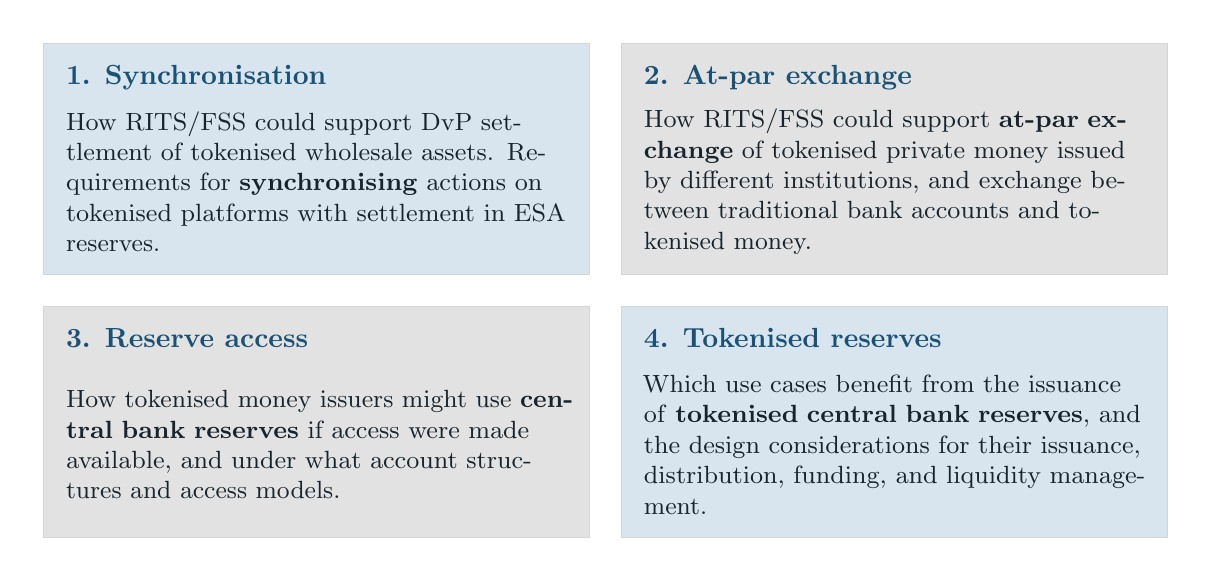
\begin{tikzpicture}[x=1cm,y=1cm]
  \useasboundingbox (0,0) rectangle (14.68,-6.68);
  \tikzset{area title/.style={anchor=north west,inner sep=0pt,text=Rust,font=\displayfont\fontsize{10.0}{12.2}\selectfont\bfseries},
    area text/.style={anchor=west,inner sep=0pt,text width=6.38cm,align=left,text=Ink,font=\fontsize{8.8}{11.0}\selectfont}}
  \filldraw[fill=DesignBlue,draw=Quiet!28!Paper,line width=.4pt] (.20,-.20) rectangle (7.14,-3.14);
  \filldraw[fill=DesignGrey,draw=Quiet!28!Paper,line width=.4pt] (7.54,-.20) rectangle (14.48,-3.14);
  \filldraw[fill=DesignGrey,draw=Quiet!28!Paper,line width=.4pt] (.20,-3.54) rectangle (7.14,-6.48);
  \filldraw[fill=DesignBlue,draw=Quiet!28!Paper,line width=.4pt] (7.54,-3.54) rectangle (14.48,-6.48);
  \node[area title] at (.48,-.47) {1. Synchronisation};
  \node[area text] at (.48,-1.955) {How RITS/FSS could support DvP settlement of tokenised wholesale assets. Requirements for \textbf{synchronising} actions on tokenised platforms with settlement in ESA reserves.};
  \node[area title] at (7.82,-.47) {2. At-par exchange};
  \node[area text] at (7.82,-1.955) {How RITS/FSS could support \textbf{at-par exchange} of tokenised private money issued by different institutions, and exchange between traditional bank accounts and tokenised money.};
  \node[area title] at (.48,-3.81) {3. Reserve access};
  \node[area text] at (.48,-5.295) {How tokenised money issuers might use \textbf{central bank reserves} if access were made available, and under what account structures and access models.};
  \node[area title] at (7.82,-3.81) {4. Tokenised reserves};
  \node[area text] at (7.82,-5.295) {Which use cases benefit from the issuance of \textbf{tokenised central bank reserves}, and the design considerations for their issuance, distribution, funding, and liquidity management.};
\end{tikzpicture}
\end{frame}
}
\fi


\iftrue % Unhidden 6 Oct 2026 (was hidden 2026-10-05: every slide before "Messaging and tokens", kept in the source.
% BEGIN tokenisation-four-meanings -- authoritative inline slide
{\setbeamercolor{background canvas}{bg=Paper}
\setbeamercolor{normal text}{bg=Paper}
\setbeamercolor{frametitle}{bg=DesignYellow}
\setbeamertemplate{background}{
\begin{tikzpicture}\useasboundingbox (0,0) rectangle (\paperwidth,\paperheight);\fill[DesignYellow] (0,\paperheight) rectangle +(\paperwidth,-1.10cm);\end{tikzpicture}}
\newcommand{\tokenpoint}[1]{\begingroup\hangindent=6pt\hangafter=1\noindent\makebox[6pt][l]{\textcolor{TokenValueBrown}{\textbullet}}#1\par\endgroup}
\begin{frame}[t]{Tokenisation}
\hyphenpenalty=10000\relax\exhyphenpenalty=10000\relax
\vspace{0.22cm}
\definecolor{TokenHeadingGrey}{HTML}{3C3C3C}
\definecolor{TokenQuadrantOrange}{HTML}{A76F3C}
\definecolor{TokenValueBrown}{HTML}{73491F}
\definecolor{TokenQuadrantDarkGrey}{HTML}{484848}
\definecolor{AtomicBurgundy}{HTML}{68263A}
\begin{tikzpicture}[remember picture,x=1cm,y=1cm]
  \useasboundingbox (0,0) rectangle (14.68,-6.68);
  \coordinate (tokenyellowcorner) at (7.54,-3.14);
  \coordinate (tokenbluecorner) at (7.14,-3.54);
  \begin{scope}[overlay]
    \fill[DesignYellow] (tokenyellowcorner) rectangle (current page.north east);
    \fill[DesignBlue] (tokenbluecorner) rectangle (current page.south west);
    \fill[DesignBlue] ([yshift=.82cm]current page.south west) rectangle (current page.south east);
    % Faint outline on the exposed edges; the band depth matches the background template above.
    \coordinate (tokenbandedge) at ([yshift=-1.10cm]current page.north west);
    \coordinate (tokenstripeedge) at ([yshift=.85cm]current page.south west);
    \draw[Quiet!22,line width=.3pt] (tokenbandedge) -- (tokenbandedge -| tokenyellowcorner) -- (tokenyellowcorner) -- (tokenyellowcorner -| current page.east);
    \draw[Quiet!22,line width=.3pt] (tokenbluecorner -| current page.west) -- (tokenbluecorner) -- (tokenbluecorner |- tokenstripeedge) -- (current page.east |- tokenstripeedge);
  \end{scope}
  \fill[Paper] (7.34,-3.34) circle[radius=2.74636cm];
  \begin{scope}
    \clip (7.34,-3.34) circle[radius=2.74636cm];
    \fill[TokenQuadrantDarkGrey,opacity=.85] (.20,-.20) rectangle (7.14,-3.14);
    \fill[TokenQuadrantOrange,opacity=.85] (7.54,-.20) rectangle (14.48,-3.14);
    \fill[Rust,opacity=.85] (.20,-3.54) rectangle (7.14,-6.48);
    \fill[TokenQuadrantDarkGrey,opacity=.85] (7.54,-3.54) rectangle (14.48,-6.48);
\end{scope}
% Thin ring outside the quadrants, carrying each quadrant colour at lower opacity.
\begin{scope}[even odd rule]
  \clip (7.34,-3.34) circle[radius=2.94cm] (7.34,-3.34) circle[radius=2.80cm];
  \fill[TokenQuadrantDarkGrey,opacity=.42] (.20,-.20) rectangle (7.14,-3.14);
  \fill[TokenQuadrantOrange,opacity=.42] (7.54,-.20) rectangle (14.48,-3.14);
  \fill[Rust,opacity=.42] (.20,-3.54) rectangle (7.14,-6.48);
  \fill[TokenQuadrantDarkGrey,opacity=.42] (7.54,-3.54) rectangle (14.48,-6.48);
  \end{scope}
  % Preserve the selected symbols: contactless bands in a circle, dollar sign, iris and filled-node hexagonal network in a circle.
  % Do not substitute card or ID-card icons during unrelated layout edits.
  % Copyright and licence notices accompany the assets and distributed PDF.
  % Radius reduced by the 0.40 cm inter-quadrant gap; icon centres follow it inward.
  \node[inner sep=0pt] at (6.194,-2.194) {\includegraphics[width=1.50cm]{figures/icons/custom/tokenisation/contactless-circle-white-thicker.pdf}};
  \node[inner sep=0pt] at (8.486,-2.194) {\includegraphics[width=1.50cm]{figures/icons/custom/tokenisation/circle-dollar-double-white-thicker.pdf}};
  \node[inner sep=0pt] at (6.194,-4.486) {\includegraphics[width=1.50cm]{figures/icons/custom/tokenisation/scan-eye-square-white-thicker.pdf}};
  \node[inner sep=0pt] at (8.486,-4.486) {\includegraphics[width=1.50cm]{figures/icons/custom/tokenisation/neural-hexagon-circle-white-thicker-filled.pdf}};
\begin{scope}[overlay]
  \tikzset{tokenblock/.style={anchor=north west,inner sep=0pt,align=justify,text width=3.70cm,text=Ink,font=\sffamily\fontsize{6.1}{6.6}\selectfont,execute at begin node={\hypersetup{urlcolor=Ink}\setlength{\parindent}{0pt}\setlength{\parskip}{.7pt}\leftskip=0pt\rightskip=0pt\parfillskip=0pt plus 1fil\relax\spaceskip=0pt\xspaceskip=0pt}},raggedtoken/.style={align=left,execute at begin node={\hypersetup{urlcolor=Ink}\setlength{\parindent}{0pt}\setlength{\parskip}{.7pt}\leftskip=0pt\raggedright\spaceskip=0pt\xspaceskip=0pt}}}
  \node[tokenblock,text width=7.45cm] at (-.10,-.057) {{\displayfont\bfseries\color{TokenQuadrantDarkGrey}\fontsize{8.8}{10.5}\selectfont Payment Tokens}\par};
  \node[tokenblock,text width=7.45cm] at (-.10,-.426) {{\displayfont\bfseries\itshape\color{TokenQuadrantDarkGrey}\fontsize{6.8}{8.0}\selectfont Substitute payment identifiers}\par};
  \node[tokenblock,text width=7.30cm,text=TokenQuadrantDarkGrey] at (-.10,-.841) {%
    {\hypersetup{urlcolor=TokenQuadrantDarkGrey}\fontsize{7.1}{7.1}\selectfont
    \parshape 12
      0cm 6.53cm 0cm 5.97cm 0cm 5.59cm 0cm 5.32cm
      0cm 5.10cm 0cm 4.94cm 0cm 4.79cm 0cm 4.68cm
      0cm 4.60cm 0cm 4.55cm 0cm 4.49cm 0cm 4.47cm
    \mbox{\textit{Tokenisation} has different meanings within payments.}\hfil\break
    \href{https://www.emvco.com/emv-technologies/payment-tokenisation/}{EMV~\textbf{payment~tokens} replace a card's primary\hfil\break account number with a cryptographic token that\hfil\break can be restricted to a device or merchant,\hfil\break limiting misuse if stolen.}
    \par}\vspace{7.5pt}{\fontsize{5.1}{5.6}\selectfont\itshape\color{TokenQuadrantDarkGrey}\hypersetup{urlcolor=TokenQuadrantDarkGrey}\parshape 1 0cm 4.40cm
    \href{https://www.emvco.com/wp-content/uploads/2023/01/EMVCo-Annual-Report_2022-FINAL.pdf}{\textbf{EMV} stands for Europay, Mastercard and Visa }\href{https://www.sec.gov/Archives/edgar/data/1141391/000095012305009470/y11299e10vq.htm}{(the three biggest card schemes before Mastercard bought Europay). }\href{https://www.emvco.com/about-us/overview-of-emvco/}{\textbf{EMVCo} was established in 1999 to develop common specifications for interoperable chip-card payments.}\par}
  };
  \node[tokenblock,text width=5.68cm] at (9.06,-.011) {{\raggedright\displayfont\bfseries\color{TokenValueBrown}\fontsize{8.8}{10.5}\selectfont Value Tokens\strut\par}};
  \node[tokenblock,text width=5.68cm] at (9.06,-.401) {{\raggedright\displayfont\bfseries\itshape\color{TokenValueBrown}\fontsize{6.8}{8.0}\selectfont On-ledger value or rights\par}};
  \node[tokenblock,text width=6.25cm,font=\sffamily\itshape\fontsize{7.1}{7.1}\selectfont] at (7.96,0.990) {\href{https://www.rba.gov.au/media-releases/2026/mr-26-24.html}{Tokenisation in the context of the \textbf{RITS consultation}\\concerns settlement involving \textbf{value tokens}.}\par};
  \node[tokenblock,text width=5.60cm,text=Rust,font=\sffamily\fontsize{7.6}{8.5}\selectfont] at (9.559,-0.871) {\hypersetup{urlcolor=Rust}\tokenpoint{\mbox{\href{https://www.esma.europa.eu/publications-and-data/interactive-single-rulebook/mica/article-3-definitions}{\textcolor{TokenValueBrown}{\textbf{E-money tokens:}} {\fontsize{6.6}{7.4}\selectfont e.g. USDC (dollar peg).}}}}};
  \node[tokenblock,text width=5.25cm,text=Rust,font=\sffamily\fontsize{7.6}{8.5}\selectfont] at (9.996,-1.351) {\hypersetup{urlcolor=Rust}\tokenpoint{\mbox{\href{https://www.esma.europa.eu/publications-and-data/interactive-single-rulebook/mica/article-3-definitions}{\textcolor{TokenValueBrown}{\textbf{Asset-referenced:}} {\fontsize{6.6}{7.4}\selectfont asset (e.g. gold) or basket.}}}}};
  \node[tokenblock,text width=5.15cm,text=Rust,font=\sffamily\fontsize{7.6}{8.5}\selectfont] at (10.270,-1.831) {\hypersetup{urlcolor=Rust}\tokenpoint{\mbox{\href{https://www.esma.europa.eu/publications-and-data/interactive-single-rulebook/mica/article-3-definitions}{\textcolor{TokenValueBrown}{\textbf{Utility:}} {\fontsize{6.6}{7.4}\selectfont issuer's service (e.g. storage credits).}}}}};
  \node[tokenblock,text width=4.90cm,text=Rust,font=\sffamily\fontsize{7.6}{8.5}\selectfont] at (10.432,-2.311) {\hypersetup{urlcolor=Rust}\tokenpoint{\mbox{\href{https://www.esma.europa.eu/sites/default/files/2025-10/Updated_Joint_ESAs_Factsheet_on_crypto-assets_CY_EN.pdf}{\textcolor{TokenValueBrown}{\textbf{Cryptocurrency:}} {\fontsize{6.6}{7.4}\selectfont Bitcoin, Ether.}}}}};
  \node[tokenblock,text width=4.20cm] at (-.10,-3.875) {%
    {\displayfont\bfseries\color{Rust}\fontsize{8.8}{10.5}\selectfont Identity Tokens\strut\par}\vspace{-1.02pt}
    {\displayfont\bfseries\itshape\color{Rust}\fontsize{6.8}{8.0}\selectfont ID claims and access rights\par}\vspace{2pt}
  };
  \node[tokenblock,raggedtoken,text width=7.00cm,text=Rust,font=\sffamily\fontsize{6.9}{7.8}\selectfont] at (-.10,-4.681) {%
    \hypersetup{urlcolor=Rust}%
    \parshape 3 0cm 4.78cm 0cm 5.02cm 0cm 5.07cm
    \href{https://openid.net/specs/openid-connect-core-1_0.html\#IDToken}{\textbf{OpenID~Connect~ID~Tokens} identify who\hfil\break signed in, using JSON Web Token (JWT) format. }\href{https://www.rfc-editor.org/rfc/rfc6749.html\#section-1.4}{\textbf{OAuth~access~tokens} authorise actions at a service.}\par
    \parshape 3 0cm 6.00cm 0cm 6.20cm 0cm 6.40cm
    \href{https://www.w3.org/TR/vc-data-model-2.0/}{\textbf{Verifiable credentials} carry signed claims a\hfil\break holder presents repeatedly rather than resupplying\hfil\break documents. }\href{https://www.rfc-editor.org/rfc/rfc9901.html}{\textbf{SD-JWT}, a selectively disclosable JWT, reveals only the claims needed.}\par
  };
  \node[tokenblock,anchor=south west,text width=14.80cm,text=Rust,font=\sffamily\itshape\bfseries\fontsize{8.0}{9.2}\selectfont] at ([xshift=.525cm,yshift=.35cm]current page.south west) {\hypersetup{urlcolor=Rust}%
    \href{https://www.w3.org/TR/did/}{Blockchains can record public keys to verify off-chain credentials. }\href{https://eips.ethereum.org/EIPS/eip-3643}{Identity tokens can govern who holds or transfers value tokens.}\par
  };
  \node[tokenblock,raggedtoken,text width=4.38cm,text=TokenQuadrantDarkGrey] at (10.58,-3.50) {%
    {\raggedright\displayfont\bfseries\color{TokenQuadrantDarkGrey}\fontsize{8.8}{10.5}\selectfont Context Tokens\strut\par}\vspace{-1.02pt}
    {\raggedright\displayfont\bfseries\itshape\color{TokenQuadrantDarkGrey}\fontsize{6.8}{8.0}\selectfont Units of data for AI\par}\vspace{3.44pt}
    {\hypersetup{urlcolor=TokenQuadrantDarkGrey}\fontsize{6.7}{7.0}\selectfont
    \href{https://ai.google.dev/gemini-api/docs/tokens}{AI models process text, images, audio and video as tokens.}
    \href{https://platform.claude.com/docs/en/build-with-claude/context-windows}{The context~window limits tokens used at once.}
    \href{https://platform.claude.com/docs/en/about-claude/pricing}{Token counts measure usage; prices reflect compute demand and supply, and may differ for input, output and cached input.}
    Token economics will likely become central to finance as autonomous agents acquire control of value tokens.
   \par}
  };
\end{scope}
\end{tikzpicture}
\end{frame}
}
% END tokenisation-four-meanings












% Opening industry slides use the same Paper background as the main deck.
{\setbeamercolor{background canvas}{bg=Paper}
\setbeamercolor{normal text}{bg=Paper}
\setbeamercolor{frametitle}{bg=Paper}
\begin{frame}[t,label=industry-payments-overview]{\makebox[\dimexpr\paperwidth-1.24cm\relax][l]{Industry ledgers\hfill{\sffamily\mdseries\fontsize{10.0}{11.8}\selectfont\color{black}Deposit tokens and repo}}}
\vspace{-0.10cm}
\fontsize{6.0}{6.4}\selectfont\renewcommand{\arraystretch}{1.0}\setlength{\tabcolsep}{1.8pt}\setlength{\extrarowheight}{0pt}
% Retain Whale as a separate platform operator; bank rows describe the linked deposit services.
% Uniform row height and shared body font; retain a clear bottom margin.
% Equal fixed-height cells; centre short entries vertically in each row.
\let\hdr\hdrmono
\begin{tabularx}{\textwidth}{K{2.35cm}YL{1.20cm}L{2.25cm}}
\hdr{Service} & \hdr{Instruments and ledger function} & \hdr{Platform} & \hdr{Reported activity} \\ \arrayrulecolor{Rust}\specialrule{0.9pt}{1pt}{0pt}\arrayrulecolor{Mist}
\parbox[c][17.0pt][c]{\linewidth}{\raggedright\lineskiplimit=-2pt\relax\strut  {\fontsize{6.0}{6.4}\selectfont \mbox{Kinexys Digital Payments}\newline\mbox{\mdseries\itshape\color{Rust} \href{https://www.jpmorgan.com/payments/newsroom/ant-international-kinexys-fx-blockchain-settlement}{2019}\quad \raisebox{-.5pt}[0pt][0pt]{\scalebox{.92}{\flag{united-states}}}}}\strut} & \parbox[c][17.0pt][c]{\linewidth}{\raggedright\lineskiplimit=-2pt\relax\strut \href{https://dcfintechweek.org/wp-content/uploads/2024/09/Application-of-Programmability-to-Commercial-Banking-and-Payments.pdf\#page=12}{\textbf{Native JPMorgan deposits}: authoritative ledger; }\href{https://www.jpmorgan.com/kinexys/blockchain-deposit-accounts}{treasury payments. }\strut} & \parbox[c][17.0pt][c]{\linewidth}{\raggedright\lineskiplimit=-2pt\relax\strut \fontsize{6.0}{6.4}\selectfont \href{https://www.jpmorgan.com/kinexys/documents/Application-of-Programmability-to-Commercial-Banking-and-Payments.pdf\#page=12}{Quorum, }\href{https://www.jpmorgan.com/kinexys/jpm-coin}{Base}\strut} & \parbox[c][17.0pt][c]{\linewidth}{\raggedright\lineskiplimit=-2pt\relax\strut  \href{https://www.jpmorgan.com/kinexys/documents/Application-of-Programmability-to-Commercial-Banking-and-Payments.pdf\#page=12}{\textbf{US\$1bn+/day}\newline Payments; 2024 report}\strut} \\ \hline
\parbox[c][17.0pt][c]{\linewidth}{\raggedright\lineskiplimit=-2pt\relax\strut  {\fontsize{6.0}{6.4}\selectfont \mbox{HQLA\textsuperscript{x}}\newline\mbox{\mdseries\itshape\color{Rust} \href{https://web.archive.org/web/20220123054931/https://www.hqla-x.com/post/commerzbank-credit-suisse-and-ubs-execute-first-live-transactions-on-the-deutsche-borse-hqlax-securities-lending-platform}{2019}\quad \raisebox{-.5pt}[0pt][0pt]{\scalebox{.92}{\flag{luxembourg}}}}}\strut} & \parbox[c][17.0pt][c]{\linewidth}{\raggedright\lineskiplimit=-2pt\relax\strut \href{https://www.sec.gov/files/tm/no-action/hqlax-nal-request-050426.pdf}{\textbf{High-quality liquid assets}: tokenised government/corporate-bond entitlements for lending, swaps and repo; ownership changes, securities stay in custody. }\href{https://www.broadridge.com/press-release/2026/hqlax-announces-strategic-investments-from-broadridge}{Canton migration planned.}\strut} & \parbox[c][17.0pt][c]{\linewidth}{\raggedright\lineskiplimit=-2pt\relax\strut \fontsize{6.0}{6.4}\selectfont \href{https://www.hqla-x.com/post/hqlax-announces-strategic-investments-from-broadridge-and-digital-asset-to-support-its-next-phase-of-growth-on-canton}{Corda}\strut} & \parbox[c][17.0pt][c]{\linewidth}{\raggedright\lineskiplimit=-2pt\relax\strut  \href{https://www.hqla-x.com/post/j-p-morgan-hqlax-and-ownera-launch-intraday-repo-solution-with-5bn-traded-in-the-first-month}{\textbf{US\$5bn intraday repo}\newline First month; Aug 2025}\strut} \\ \hline
\parbox[c][17.0pt][c]{\linewidth}{\raggedright\lineskiplimit=-2pt\relax\strut  {\fontsize{6.0}{6.4}\selectfont \mbox{Broadridge DLR}\newline\mbox{\mdseries\itshape\color{Rust} 2021\quad \raisebox{-.5pt}[0pt][0pt]{\scalebox{.92}{\flag{united-states}}}}}\strut} & \parbox[c][17.0pt][c]{\linewidth}{\raggedright\lineskiplimit=-2pt\relax\strut \href{https://www.broadridge.com/press-release/2026/broadridge-brings-g7-securities-to-institutional-tokenized-repo}{\textbf{Distributed Ledger Repo}: US Treasury repo, intraday repo and collateral pledges; }\href{https://www.broadridge.com/_assets/pdf/broadridge-distributed-ledger-repo-enters-its-next-phase.pdf}{tokenised ownership transfers, securities stay in custody. }\href{https://www.broadridge.com/press-release/2026/broadridge-brings-g7-securities-to-institutional-tokenized-repo}{G7 collateral expansion announced Sep 2026.}\strut} & \parbox[c][17.0pt][c]{\linewidth}{\raggedright\lineskiplimit=-2pt\relax\strut \fontsize{6.0}{6.4}\selectfont \href{https://www.broadridge.com/insights/dlr-transacts-1-trillion-a-month}{Canton}\strut} & \parbox[c][17.0pt][c]{\linewidth}{\raggedright\lineskiplimit=-2pt\relax\strut  \href{https://www.broadridge.com/press-release/2026/broadridge-brings-g7-securities-to-institutional-tokenized-repo}{\textbf{US\$351bn/day}\newline Mean repo; Aug 2026}\strut} \\ \hline
\parbox[c][17.0pt][c]{\linewidth}{\raggedright\lineskiplimit=-2pt\relax\strut  {\fontsize{6.0}{6.4}\selectfont \mbox{Partior}\newline\mbox{\mdseries\itshape\color{Rust} \href{https://www.dbs.com/annualreports/2021/files/media/dbs-annual-report-2021.pdf\#page=10}{2021}\quad \raisebox{-.5pt}[0pt][0pt]{\scalebox{.92}{\flag{singapore}}}}}\strut} & \parbox[c][17.0pt][c]{\linewidth}{\raggedright\lineskiplimit=-2pt\relax\strut  \href{https://partior.com/news-and-insights/dbs-j-p-morgan-and-temasek-to-establish-platform-to-transform-interbank-value-movements-in-a-new-digital-era}{\textbf{Interbank payments in tokenised commercial bank money} }\href{https://partior.com/news-and-insights/sooho-io-and-partior-partner-to-connect-korean-financial-institutions-to-live-global-settlement-rails}{(USD/EUR/SGD); }\href{https://partior.com/solutions/partior-payments}{banks only, 24/7. }\href{https://partior.com/news-and-insights/dbs-j-p-morgan-and-temasek-to-establish-platform-to-transform-interbank-value-movements-in-a-new-digital-era}{Founders: DBS, J.P. Morgan, Temasek. }\strut} & \parbox[c][17.0pt][c]{\linewidth}{\raggedright\lineskiplimit=-2pt\relax\strut  \href{https://dcfintechweek.org/wp-content/uploads/2024/09/Application-of-Programmability-to-Commercial-Banking-and-Payments.pdf\#page=13}{Quorum}\strut} & \parbox[c][17.0pt][c]{\linewidth}{\raggedright\lineskiplimit=-2pt\relax\strut  \href{https://partior.com/news-and-insights/partior-welcomes-deutsche-bank-as-strategic-investor}{\textbf{US\$1bn+ transferred}\newline Cumulative; Nov 2024}\strut} \\ \hline
\parbox[c][17.0pt][c]{\linewidth}{\raggedright\lineskiplimit=-2pt\relax\strut  {\fontsize{6.0}{6.4}\selectfont \mbox{\href{https://fnality.com/payment-systems/british-sterling-payment-system}{Fnality \pounds FnPS}}\newline\mbox{\mdseries\itshape\color{Rust} \href{https://fnality.com/news/fnality-commences-initial-phase-of-sterling-payment-operations-in-a-world-first}{2023}\quad \raisebox{-.5pt}[0pt][0pt]{\scalebox{.92}{\flag{united-kingdom}}}}}\strut} & \parbox[c][17.0pt][c]{\linewidth}{\raggedright\lineskiplimit=-2pt\relax\strut \href{https://fnality.com/news/the-liquidity-myth-why-everything-on-chain-doesnt-work-for-wholesale-settlement}{\textbf{Fnality Payment System}: native sterling wholesale balances on the authoritative ledger, }\href{https://fnality.com/how-it-works}{backed by Bank of England funds; }\href{https://fnality.com/news/earmarked-funds}{earmarking supports conditional payments.}\strut} & \parbox[c][17.0pt][c]{\linewidth}{\raggedright\lineskiplimit=-2pt\relax\strut \fontsize{6.0}{6.4}\selectfont \href{https://fnality.com/news/fnality-and-ethereum-alliance}{Besu}\strut} & \parbox[c][17.0pt][c]{\linewidth}{\raggedright\lineskiplimit=-2pt\relax\strut  \href{https://www.bankofengland.co.uk/financial-stability/financial-market-infrastructure-supervision/report/fmi-annual-report-2025-26}{\textbf{Aggregate unavailable}\newline Payment value}\strut} \\ \hline
\parbox[c][17.0pt][c]{\linewidth}{\raggedright\lineskiplimit=-2pt\relax\strut  {\fontsize{6.0}{6.4}\selectfont \mbox{Whale (Ant International)}\newline\mbox{\mdseries\itshape\color{Rust} \href{https://www.ant-intl.com/en/ant-intl_SR2024.pdf\#page=5}{2024}\quad \raisebox{-.5pt}[0pt][0pt]{\scalebox{.92}{\flag{singapore}}}}}\strut} & \parbox[c][17.0pt][c]{\linewidth}{\raggedright\lineskiplimit=-2pt\relax\strut  \href{https://www.ant-intl.com/en/ant-intl_SR2024.pdf}{\textbf{Ant group treasury:} blockchain platform connecting partner-bank deposit services; 24/7 intra-group transfers. }\href{https://www.jpmorgan.com/payments/newsroom/ant-international-kinexys-fx-blockchain-settlement}{FX via Kinexys.}\strut} & \parbox[c][17.0pt][c]{\linewidth}{\raggedright\lineskiplimit=-2pt\relax\strut \fontsize{6.0}{6.4}\selectfont \href{https://junmtan.dev/}{Besu}\strut} & \parbox[c][17.0pt][c]{\linewidth}{\raggedright\lineskiplimit=-2pt\relax\strut  \href{https://www.antom.com/news/ant-international-powered-over-2-billion-transactions-in-its-core-emerging-markets-in-2025}{\textbf{US\$600bn+ processed}\newline Period unstated; Jan 2026}\strut} \\ \hline
\parbox[c][17.0pt][c]{\linewidth}{\raggedright\lineskiplimit=-2pt\relax\strut  {\fontsize{6.0}{6.4}\selectfont \mbox{Citi Token Services}\newline\mbox{\mdseries\itshape\color{Rust} \href{https://www.lfdecentralizedtrust.org/case-studies/citi-transforms-transaction-banking-services-with-besu}{2024}\quad \raisebox{-.5pt}[0pt][0pt]{\scalebox{.92}{\flag{united-states}}}}}\strut} & \parbox[c][17.0pt][c]{\linewidth}{\raggedright\lineskiplimit=-2pt\relax\strut \href{https://www.citigroup.com/rcs/citigpa/storage/public/RealTime_Liquidity_Solutions.pdf\#page=3}{\textbf{Citi Token Services for Cash}: tokens record liabilities between Citi branches, not customer deposit claims. }\href{https://services.citi.com/solutions/citi-token-services}{24/7 liquidity transfers, subject to limits; }\href{https://www.citigroup.com/rcs/citigpa/storage/public/investor-day/citi-ID26-services-presentation-transcript.pdf}{liquidity and working-capital management.}\strut} & \parbox[c][17.0pt][c]{\linewidth}{\raggedright\lineskiplimit=-2pt\relax\strut \fontsize{6.0}{6.4}\selectfont \href{https://www.lfdecentralizedtrust.org/case-studies/citi-transforms-transaction-banking-services-with-besu}{Besu}\strut} & \parbox[c][17.0pt][c]{\linewidth}{\raggedright\lineskiplimit=-2pt\relax\strut  \href{https://www.citigroup.com/rcs/citigpa/storage/public/investor-day/citi-ID26-services-presentation-transcript.pdf}{\textbf{\textasciitilde{}US\$1bn/day}\newline Mean flow; May 2026}\strut} \\ \hline
\parbox[c][17.0pt][c]{\linewidth}{\raggedright\lineskiplimit=-2pt\relax\strut  {\fontsize{6.0}{6.4}\selectfont \mbox{DBS Token Services}\newline\mbox{\mdseries\itshape\color{Rust} \href{https://www.dbs.com/newsroom/DBS_rolls_out_blockchain_powered_banking_for_institutions_with_DBS_Token_Services_marks_new_milestone_in_financial_services}{2024}\quad \raisebox{-.5pt}[0pt][0pt]{\scalebox{.92}{\flag{singapore}}}}}\strut} & \parbox[c][17.0pt][c]{\linewidth}{\raggedright\lineskiplimit=-2pt\relax\strut \href{https://www.dbs.com/newsroom/DBS_rolls_out_blockchain_powered_banking_for_institutions_with_DBS_Token_Services_marks_new_milestone_in_financial_services}{\textbf{DBS (Development Bank of Singapore)}: deposit tokens and programmable 24/7 treasury payments; }\href{https://www.dbs.com/newsroom/DBS_launches_blockchain_powered_Treasury_Tokens_pilot_with_Ant_International_for_247_treasury_and_liquidity_management}{private Ethereum Virtual Machine-compatible ledger linked to Ant\textquotesingle s Whale.}\strut} & \parbox[c][17.0pt][c]{\linewidth}{\raggedright\lineskiplimit=-2pt\relax\strut \fontsize{6.0}{6.4}\selectfont \href{https://www.dbs.com/newsroom/DBS_rolls_out_blockchain_powered_banking_for_institutions_with_DBS_Token_Services_marks_new_milestone_in_financial_services}{Private EVM}\strut} & \parbox[c][17.0pt][c]{\linewidth}{\raggedright\lineskiplimit=-2pt\relax\strut  \href{https://www.dbs.com/annualreports/2025/institutional-banking.html}{\textbf{Aggregate unavailable}\newline Payment value}\strut} \\ \hline
\parbox[c][17.0pt][c]{\linewidth}{\raggedright\lineskiplimit=-2pt\relax\strut  {\fontsize{6.0}{6.4}\selectfont \mbox{HSBC TDS}\newline\mbox{\mdseries\itshape\color{Rust} \href{https://www.about.hsbc.com.hk/news-and-media/hsbc-launches-tokenised-deposit-service-for-corporate-cash-management-in-hong-kong}{2025}\quad \raisebox{-.5pt}[0pt][0pt]{\scalebox{.92}{\flag{united-kingdom}}}}}\strut} & \parbox[c][17.0pt][c]{\linewidth}{\raggedright\lineskiplimit=-2pt\relax\strut \href{https://www.business.hsbc.com/en-gb/products/tokenised-deposit-service}{\textbf{Tokenised Deposit Service}: HSBC deposit representations using private distributed ledger technology; 24/7 corporate wallet transfers. }\href{https://www.sc.com/en/press-release/standard-chartered-and-hsbc-execute-first-live-tokenised-deposit-transaction-on-swifts-blockchain-based-ledger/}{Six markets / seven currencies by Aug 2026.}\strut} & \parbox[c][17.0pt][c]{\linewidth}{\raggedright\lineskiplimit=-2pt\relax\strut \fontsize{6.0}{6.4}\selectfont Private DLT\strut} & \parbox[c][17.0pt][c]{\linewidth}{\raggedright\lineskiplimit=-2pt\relax\strut  \href{https://www.hsbc.com/-/files/hsbc/investors/investing-in-hsbc/investor-events-and-presentations/2026/260521-global-payments-solutions-presentation.pdf}{\textbf{\textasciitilde{}US\$28bn}\newline Payments; Q1 2026}\strut} \\ \hline
\parbox[c][17.0pt][c]{\linewidth}{\raggedright\lineskiplimit=-2pt\relax\strut  {\fontsize{6.0}{6.4}\selectfont \mbox{Standard Chartered}\newline\mbox{\mdseries\itshape\color{Rust} \href{https://www.sc.com/en/press-release/standard-chartered-launches-blockchain-based-tokenised-deposits-solution-in-sgd-and-usd/}{2025}\quad \raisebox{-.5pt}[0pt][0pt]{\scalebox{.92}{\flag{united-kingdom}}}}}\strut} & \parbox[c][17.0pt][c]{\linewidth}{\raggedright\lineskiplimit=-2pt\relax\strut  \href{https://www.sc.com/en/press-release/standard-chartered-launches-blockchain-based-tokenised-deposits-solution-in-sgd-and-usd/}{\textbf{Tokenised bank deposits}: SGD/USD balances on Ant\textquotesingle s Whale platform; 24/7 intra-group treasury transfers, with additional HKD/CNH capabilities.}\strut} & \parbox[c][17.0pt][c]{\linewidth}{\raggedright\lineskiplimit=-2pt\relax\strut  \href{https://www.sc.com/en/press-release/standard-chartered-launches-blockchain-based-tokenised-deposits-solution-in-sgd-and-usd/}{Private DLT}\strut} & \parbox[c][17.0pt][c]{\linewidth}{\raggedright\lineskiplimit=-2pt\relax\strut  \href{https://www.sc.com/en/press-release/standard-chartered-launches-blockchain-based-tokenised-deposits-solution-in-sgd-and-usd/}{\textbf{Aggregate unavailable}\newline Payment value}\strut} \\ \hline
\parbox[c][17.0pt][c]{\linewidth}{\raggedright\lineskiplimit=-2pt\relax\strut  {\fontsize{6.0}{6.4}\selectfont \mbox{BNY tokenised deposits}\newline\mbox{\mdseries\itshape\color{Rust} \href{https://www.bny.com/corporate/global/en/about-us/newsroom/company-news/bny-extends-digital-cash-capabilities-for-institutional-clients.html}{2026}\quad \raisebox{-.5pt}[0pt][0pt]{\scalebox{.92}{\flag{united-states}}}}}\strut} & \parbox[c][17.0pt][c]{\linewidth}{\raggedright\lineskiplimit=-2pt\relax\strut \href{https://www.bny.com/corporate/global/en/about-us/newsroom/company-news/bny-extends-digital-cash-capabilities-for-institutional-clients.html}{\textbf{Bank of New York Mellon deposit mirrors}: }\href{https://www.bny.com/corporate/global/en/about-us/newsroom/company-news/bny-extends-digital-cash-capabilities-for-institutional-clients.html}{private ledger for collateral and margin workflows; authoritative deposit records remain off-chain.}\strut} & \parbox[c][17.0pt][c]{\linewidth}{\raggedright\lineskiplimit=-2pt\relax\strut  Private DLT\strut} & \parbox[c][17.0pt][c]{\linewidth}{\raggedright\lineskiplimit=-2pt\relax\strut  \href{https://www.bny.com/corporate/global/en/about-us/newsroom/company-news/bny-extends-digital-cash-capabilities-for-institutional-clients.html}{\textbf{Aggregate unavailable}\newline Payment value}\strut} \\ \arrayrulecolor{Rust}\specialrule{0.5pt}{0pt}{0pt}
\end{tabularx}\par
\end{frame}



\begin{frame}[t,label=industry-securities-overview]{\makebox[\dimexpr\paperwidth-1.24cm\relax][l]{Industry ledgers\hfill{\sffamily\mdseries\fontsize{10.0}{11.8}\selectfont\color{black}Securities, funds \& loans}}}
\vspace{-0.28em}
\fontsize{6.0}{7.2}\selectfont\renewcommand{\arraystretch}{1.0}\setlength{\tabcolsep}{2pt}\setlength{\extrarowheight}{0pt}
\let\hdr\hdrmono
\begin{tabularx}{\textwidth}{K{2.30cm}YL{1.50cm}L{2.30cm}}
\hdr{Service} & \hdr{Instruments and ledger function} & \hdr{Platform} & \hdr{Reported activity} \\ \arrayrulecolor{Rust}\specialrule{0.9pt}{1pt}{0pt}\arrayrulecolor{Mist}
\parbox[c][18.86pt][c]{\linewidth}{\raggedright {\fontsize{6.1}{7.5}\selectfont \mbox{Figure}\newline\mbox{\mdseries\itshape\color{Rust} \href{https://www.sec.gov/Archives/edgar/data/2064124/000162828025052613/figr-20251117.htm}{2018}\quad \raisebox{-.5pt}[0pt][0pt]{\scalebox{.92}{\flag{united-states}}}}}} & \parbox[c][18.86pt][c]{\linewidth}{\raggedright \href{https://www.sec.gov/Archives/edgar/data/2064124/000162828025052613/figr-20251117.htm}{\textbf{Loans, including home equity lines of credit (HELOCs)}; origination, ownership, liens and sales. DART loan register; Figure Connect trading and settlement.}} & \parbox[c][18.86pt][c]{\linewidth}{\raggedright \href{https://www.sec.gov/Archives/edgar/data/2064124/000162828025052613/figr-20251117.htm}{Provenance}} & \parbox[c][18.86pt][c]{\linewidth}{\raggedright \href{https://investors.figure.com/news-releases/news-release-details/figure-technology-solutions-reports-strong-second-quarter-2026}{\textbf{\textasciitilde{}US\$4.3bn}\newline Loan market; Q2 2026}} \\ \hline
\parbox[c][18.86pt][c]{\linewidth}{\raggedright {\fontsize{6.1}{7.5}\selectfont \mbox{Ant Digital}\newline\mbox{\mdseries\itshape\color{Rust} \href{https://intl.antdigital.com/en/company/milestones}{2018}\quad \raisebox{-.5pt}[0pt][0pt]{\scalebox{.92}{\flag{china}}}}}} & \parbox[c][18.86pt][c]{\linewidth}{\raggedright \href{https://www.antdigital.com/solutions}{\textbf{AntChain financial networks}: receivables, trade finance, asset-backed securities, leasing and asset tokenisation; }\href{https://www.antdigital.com/products/baas}{shared records, transfers and financing.}} & \parbox[c][18.86pt][c]{\linewidth}{\raggedright \href{https://www.antdigital.com/products/baas}{AntChain}} & \parbox[c][18.86pt][c]{\linewidth}{\raggedright \href{https://cn.linkedin.com/company/antdigitaltechnologies}{\textbf{32.4\% market share}\newline China BaaS; 2025}} \\ \hline
\parbox[c][18.86pt][c]{\linewidth}{\raggedright {\fontsize{6.1}{7.5}\selectfont \mbox{Cashlink}\newline\mbox{\mdseries\itshape\color{Rust} \href{https://cashlink.de/wp-content/uploads/2021/12/Cashlink_PM_eWpG_Lizenz.pdf}{2019}\quad \raisebox{-.5pt}[0pt][0pt]{\scalebox{.92}{\flag{germany}}}}}} & \parbox[c][18.86pt][c]{\linewidth}{\raggedright \href{https://cashlink.de/en/core/}{\textbf{Crypto-securities register}: bonds and fund units under the German Electronic Securities Act; issuance, ownership records and lifecycle management on public blockchains.}} & \parbox[c][18.86pt][c]{\linewidth}{\raggedright \href{https://cashlink.de/de/kwp-register-rechtliches-2/}{Ethereum,\newline\mbox{Polygon, Stellar}}} & \parbox[c][18.86pt][c]{\linewidth}{\raggedright \href{https://cashlink.de/wp-content/uploads/2026/08/Cashlink-partners-with-Ava-labs-to-bring-regulated-tokenization-to-Avalanche.pdf}{\textbf{EUR1bn+ transactions}\newline Cumulative; Aug 2026}} \\ \hline
\parbox[c][18.86pt][c]{\linewidth}{\raggedright {\fontsize{6.1}{7.5}\selectfont \mbox{IZNES}\newline\mbox{\mdseries\itshape\color{Rust} \href{https://iznes.io/en/presentation-entreprise/}{2019}\quad \raisebox{-.5pt}[0pt][0pt]{\scalebox{.92}{\flag{france}}}}}} & \parbox[c][18.86pt][c]{\linewidth}{\raggedright \href{https://iznes.io/en/la-plateforme-iznes/}{\textbf{Fund-unit register}: subscriptions, redemptions, ownership and servicing; }\href{https://iznes.io/en/presentation-entreprise/}{money-market, securities, real-estate and private-equity funds. Euroclear is a shareholder.}} & \parbox[c][18.86pt][c]{\linewidth}{\raggedright \href{https://iznes.io/en/presentation-entreprise/}{Hyperledger Fabric}} & \parbox[c][18.86pt][c]{\linewidth}{\raggedright \href{https://www.boursorama.com/bourse/actualites-amp/iznes-franchit-le-seuil-des-32-milliards-d-euros-d-actifs-tokenises-446b40948a317fd3cec78893ddd2abd3}{\textbf{EUR32bn registered}\newline Fund assets; May 2026}} \\ \hline
\parbox[c][18.86pt][c]{\linewidth}{\raggedright {\fontsize{6.1}{7.5}\selectfont \mbox{SWIAT}\newline\mbox{\mdseries\itshape\color{Rust} \href{https://www.swiat.io/about-us/press/}{2020}\quad \raisebox{-.5pt}[0pt][0pt]{\scalebox{.92}{\flag{germany}}}}}} & \parbox[c][18.86pt][c]{\linewidth}{\raggedright \href{https://press.siemens.com/global/en/pressrelease/siemens-remains-pioneer-another-digital-bond-successfully-issued-blockchain}{\textbf{Secure Worldwide Interbank Asset Transfer}: bonds, commercial paper and securities lending; appointed registrar maintains the register under the German Electronic Securities Act.}} & \parbox[c][18.86pt][c]{\linewidth}{\raggedright \href{https://www.swiat.io/technology/}{Besu}} & \parbox[c][18.86pt][c]{\linewidth}{\raggedright \href{https://www.swiat.io/media/press_releaes_ewpg_en_20251120.pdf}{\textbf{EUR600m+ settled}\newline Cumulative; Nov 2025}} \\ \hline
\parbox[c][18.86pt][c]{\linewidth}{\raggedright {\fontsize{6.1}{7.5}\selectfont \mbox{ADDX}\newline\mbox{\mdseries\itshape\color{Rust} \href{https://addx.co/files/ADDX_to_Appoint_New_CEO_Oi_Yee_Choo_96b346a204.pdf}{2020}\quad \raisebox{-.5pt}[0pt][0pt]{\scalebox{.92}{\flag{singapore}}}}}} & \parbox[c][18.86pt][c]{\linewidth}{\raggedright \href{https://documents.addx.co/ADDX_Connecting_Regulated_Digital_Asset_Platforms_To_Public_Blockchains.pdf}{\textbf{Private-market securities}: tokenised funds, equity and debt; issuance, custody and secondary trading on a private permissioned ledger.}} & \parbox[c][18.86pt][c]{\linewidth}{\raggedright \href{https://documents.addx.co/ADDX_Connecting_Regulated_Digital_Asset_Platforms_To_Public_Blockchains.pdf}{Private Ethereum}} & \parbox[c][18.86pt][c]{\linewidth}{\raggedright \href{https://addx.co/en/}{\textbf{SGD2bn+ transactions}\newline Total; Oct 2026}} \\ \hline
\parbox[c][18.86pt][c]{\linewidth}{\raggedright {\fontsize{6.1}{7.5}\selectfont \mbox{Kinexys Digital Assets}\newline\mbox{\mdseries\itshape\color{Rust} \href{https://www.jpmorgan.com/kinexys/documents/JPMC-Kinexys-Project-Epic-Whitepaper-2024.pdf}{2020}\quad \raisebox{-.5pt}[0pt][0pt]{\scalebox{.92}{\flag{united-states}}}}}} & \parbox[c][18.86pt][c]{\linewidth}{\raggedright \href{https://www.jpmorgan.com/technology/technology-blog/first-live-municipal-blockchain-based-bond-issuance-in-US}{\textbf{Bonds and funds}: Digital Debt Service issuance and servicing; }\href{https://www.jpmorgan.com/kinexys/fund-flow}{Fund Flow investor registers, capital calls and distributions; }\href{https://www.jpmorgan.com/kinexys/digital-financing}{intraday repo }\href{https://www.jpmorgan.com/kinexys/digital-assets/tokenized-collateral-network}{and tokenised collateral transfers.}} & \parbox[c][18.86pt][c]{\linewidth}{\raggedright \href{https://www.jpmorgan.com/kinexys/documents/JPMC-Kinexys-Project-Epic-Whitepaper-2024.pdf}{Private Ethereum}} & \parbox[c][18.86pt][c]{\linewidth}{\raggedright \href{https://www.jpmorgan.com/kinexys/documents/JPMC-Kinexys-Project-Epic-Whitepaper-2024.pdf}{\textbf{US\$2--3bn/day}\newline Asset transfers; Nov 2024}} \\ \hline
\parbox[c][18.86pt][c]{\linewidth}{\raggedright {\fontsize{6.1}{7.5}\selectfont \mbox{Clearstream FundsDLT}\newline\mbox{\mdseries\itshape\color{Rust} \href{https://www.luxse.com/about-us/press-centre/Launching-FundsDLT}{2020}\quad \raisebox{-.5pt}[0pt][0pt]{\scalebox{.92}{\flag{luxembourg}}}}}} & \parbox[c][18.86pt][c]{\linewidth}{\raggedright \href{https://www.clearstream.com/clearstream-en/newsroom/260622-5343058}{\textbf{Digital Transfer Agency}: blockchain fund register for issuance, investor ownership, subscriptions, redemptions and servicing; integrated into Clearstream Fund Services.}} & \parbox[c][18.86pt][c]{\linewidth}{\raggedright \href{https://www.fundsdlt.net/wp-content/uploads/2025/03/FundsDLT_whitepaper.pdf\#page=24}{Quorum}} & \parbox[c][18.86pt][c]{\linewidth}{\raggedright \href{https://www.clearstream.com/clearstream-en/newsroom/260622-5343058}{\textbf{EUR11bn+ processed}\newline Digital funds; Jun 2026}} \\ \hline
\parbox[c][18.86pt][c]{\linewidth}{\raggedright {\fontsize{6.1}{7.5}\selectfont \mbox{SIX Digital Asset Platform}\newline\mbox{\mdseries\itshape\color{Rust} \href{https://www.six-group.com/en/newsroom/media-releases/2021/20211118-six-sdx-digital-bond.html}{2021}\quad \raisebox{-.5pt}[0pt][0pt]{\scalebox{.92}{\flag{switzerland}}}}}} & \parbox[c][18.86pt][c]{\linewidth}{\raggedright \href{https://www.six-group.com/en/products-services/securities-services/digital-assets/digital-securities.html}{\textbf{Swiss Infrastructure and Exchange}: former SIX Digital Exchange ledger for Swiss cantonal/municipal, supranational and bank bonds and private-share depositary receipts.}} & \parbox[c][18.86pt][c]{\linewidth}{\raggedright \href{https://r3.com/unlocking-new-opportunities-to-leverage-blockchain-mitigating-settlement-risk-and-optimizing-collateral-management/}{Corda}} & \parbox[c][18.86pt][c]{\linewidth}{\raggedright \href{https://www.six-group.com/dam/download/company/report/annual/2025/six-annual-report-2025-en.pdf\#page=14}{\textbf{CHF1.5bn+ issued}\newline Cumulative; 2025 report}} \\ \hline
\parbox[c][18.86pt][c]{\linewidth}{\raggedright {\fontsize{6.1}{7.5}\selectfont \mbox{Progmat ST}\newline\mbox{\mdseries\itshape\color{Rust} \href{https://note.com/progmat/n/n96a520f32442}{2021}\quad \raisebox{-.5pt}[0pt][0pt]{\scalebox{.92}{\flag{japan}}}}}} & \parbox[c][18.86pt][c]{\linewidth}{\raggedright \href{https://progmat.co.jp/en/news/2026-07-13-press_en/}{\textbf{Security tokens}: real-estate trust interests, bonds and funds. Full ledger migration from Corda to Avalanche completed Jul 2026.}} & \parbox[c][18.86pt][c]{\linewidth}{\raggedright \href{https://progmat.co.jp/en/news/2026-07-13-press_en/}{Avalanche}} & \parbox[c][18.86pt][c]{\linewidth}{\raggedright \href{https://speakerdeck.com/progmat/progmat-monthly-st-market-report-2026-jul?slide=52}{\textbf{JPY248.1bn disclosed}\newline Issued/planned; Jul 2026}} \\ \arrayrulecolor{Rust}\specialrule{0.5pt}{0pt}{0pt}
\end{tabularx}\par
\end{frame}

\begin{frame}[t,label=industry-securities-overview-continued]{\makebox[\dimexpr\paperwidth-1.24cm\relax][l]{Industry ledgers\hfill{\sffamily\mdseries\fontsize{10.0}{11.8}\selectfont\color{black}Securities, funds \& loans}}}
\vspace{-0.28em}
\fontsize{6.0}{7.2}\selectfont\renewcommand{\arraystretch}{1.0}\setlength{\tabcolsep}{2pt}\setlength{\extrarowheight}{0pt}
\let\hdr\hdrmono
\begin{tabularx}{\textwidth}{K{2.30cm}YL{1.50cm}L{2.30cm}}
\hdr{Service} & \hdr{Instruments and ledger function} & \hdr{Platform} & \hdr{Reported activity} \\ \arrayrulecolor{Rust}\specialrule{0.9pt}{1pt}{0pt}\arrayrulecolor{Mist}
\parbox[c][18.86pt][c]{\linewidth}{\raggedright {\fontsize{6.1}{7.5}\selectfont \mbox{ibet for Fin (BOOSTRY)}\newline\mbox{\mdseries\itshape\color{Rust} \href{https://www.sbigroup.co.jp/english/investors/disclosure/presentation/pdf/210729presentations.pdf}{2021}\quad \raisebox{-.5pt}[0pt][0pt]{\scalebox{.92}{\flag{japan}}}}}} & \parbox[c][18.86pt][c]{\linewidth}{\raggedright \href{https://global.nomura-am.co.jp/media/pdf/20251202_EBEB07BF.pdf}{\textbf{Consortium securities ledger} for bonds, shares and fund interests; ownership records and transfers shared across brokers and trust banks.}} & \parbox[c][18.86pt][c]{\linewidth}{\raggedright \href{https://github.com/BoostryJP/ibet-Core}{ibet-Core} (EVM)} & \parbox[c][18.86pt][c]{\linewidth}{\raggedright \href{https://speakerdeck.com/progmat/progmat-monthly-st-market-report-2026-jul?slide=52}{\textbf{JPY133.2bn disclosed}\newline Issued/planned; Jul 2026}} \\ \hline
\parbox[c][18.86pt][c]{\linewidth}{\raggedright {\fontsize{6.1}{7.5}\selectfont \mbox{Goldman Sachs DAP}\newline\mbox{\mdseries\itshape\color{Rust} \href{https://www.eib.org/en/press/all/2022-448-eib-innovates-further-with-project-venus-the-first-euro-denominated-digital-bond-on-a-private-blockchain}{2022}\quad \raisebox{-.5pt}[0pt][0pt]{\scalebox{.92}{\flag{united-states}}}}}} & \parbox[c][18.86pt][c]{\linewidth}{\raggedright \href{https://www.eib.org/en/press/all/2022-448-eib-innovates-further-with-project-venus-the-first-euro-denominated-digital-bond-on-a-private-blockchain}{\textbf{Digital Asset Platform}: native EIB / Hong Kong Government bonds; }\href{https://www.bny.com/corporate/global/en/about-us/newsroom/company-news/bny-and-goldman-sachs-launch-tokenized-money-market-funds-solution.html}{Bank of New York Mellon money-market-fund mirrors; bank keeps official books and settlement.}} & \parbox[c][18.86pt][c]{\linewidth}{\raggedright \href{https://blog.digitalasset.com/press-release/goldman-sachs-tokenization-platform-gs-dap-leveraging-daml-goes-live}{Canton}} & \parbox[c][18.86pt][c]{\linewidth}{\raggedright \href{https://www.eib.org/en/press/all/2022-448-eib-innovates-further-with-project-venus-the-first-euro-denominated-digital-bond-on-a-private-blockchain}{\textbf{Aggregate unavailable}\newline Issuance / fund records}} \\ \hline
\parbox[c][18.86pt][c]{\linewidth}{\raggedright {\fontsize{6.1}{7.5}\selectfont \mbox{Euroclear D-FMI}\newline\mbox{\mdseries\itshape\color{Rust} \href{https://www.euroclear.com/newsandinsights/en/press/2023/2023-mr-14-euroclear-launches-dlt-solution.html}{2023}\quad \raisebox{-.5pt}[0pt][0pt]{\scalebox{.92}{\flag{belgium}}}}}} & \parbox[c][18.86pt][c]{\linewidth}{\raggedright \href{https://www.euroclear.com/newsandinsights/en/press/2023/2023-mr-14-euroclear-launches-dlt-solution.html}{\textbf{Digital Financial Market Infrastructure}: bank/supranational Digitally Native Notes, including World Bank; no sovereigns yet. Secondary settlement: Euroclear Bank\textquotesingle s existing platform.}} & \parbox[c][18.86pt][c]{\linewidth}{\raggedright \href{https://www.ecb.europa.eu/pub/pdf/other/ecb.exploratoryworknewtechnologies202506_annex02.en.pdf\#page=48}{Corda}} & \parbox[c][18.86pt][c]{\linewidth}{\raggedright \href{https://www.euroclear.com/newsandinsights/en/press/2026/mr-06-euroclear-delivers-strong-2025-results.html}{\textbf{\textasciitilde{}EUR1.2bn}\newline Issued; FY2025 report}} \\ \hline
\parbox[c][18.86pt][c]{\linewidth}{\raggedright {\fontsize{6.1}{7.5}\selectfont \mbox{HSBC Orion}\newline\mbox{\mdseries\itshape\color{Rust} \href{https://www.business.hsbc.com/-/media/media/gbm-global/pdf/articles/reinventing-assets-article-redesign.pdf}{2023}\quad \raisebox{-.5pt}[0pt][0pt]{\scalebox{.92}{\flag{luxembourg}}}}}} & \parbox[c][18.86pt][c]{\linewidth}{\raggedright \href{https://www.business.hsbc.com/-/media/media/gbm-global/pdf/articles/reinventing-assets-article-redesign.pdf}{\textbf{Sovereign/supranational bonds}; }\href{https://www.hsbc.com/news-and-views/news/media-releases/2026/hsbc-orion-awarded-digit-platform-mandate}{UK Digital Gilt Instrument (DIGIT) mandate. }\href{https://www.business.hsbc.com/-/media/media/gbm-global/pdf/articles/reinventing-assets-article-redesign.pdf}{Luxembourg: Fabric register; public Ethereum mirror tokens have no bond rights.}} & \parbox[c][18.86pt][c]{\linewidth}{\raggedright \href{https://www.business.hsbc.com/-/media/media/gbm-global/pdf/articles/reinventing-assets-article-redesign.pdf}{Hyperledger Fabric}} & \parbox[c][18.86pt][c]{\linewidth}{\raggedright \href{https://www.business.hsbc.com/en-gb/insights/hsbc-approved-for-digital-securities-sandbox}{\textbf{US\$5bn+ issued}\newline Cumulative; Jul 2026}} \\ \hline
\parbox[c][18.86pt][c]{\linewidth}{\raggedright {\fontsize{6.1}{7.5}\selectfont \mbox{Clearstream D7 DLT}\newline\mbox{\mdseries\itshape\color{Rust} \href{https://www.clearstream.com/clearstream-en/newsroom/251104-4757900}{2025}\quad \raisebox{-.5pt}[0pt][0pt]{\scalebox{.92}{\flag{luxembourg}}}}}} & \parbox[c][18.86pt][c]{\linewidth}{\raggedright \href{https://www.clearstream.com/clearstream-en/newsroom/251104-4757900}{\textbf{Commercial paper / medium-term notes}; }\href{https://www.clearstream.com/clearstream-en/newsroom/260629-5355756}{European Investment Bank paper as Eurosystem collateral (Jun 2026). }\href{https://www.clearstream.com/clearstream-en/newsroom/251104-4757900}{Clearstream Banking (Luxembourg): issuer central securities depository.}} & \parbox[c][18.86pt][c]{\linewidth}{\raggedright \href{https://www.ecb.europa.eu/pub/pdf/other/ecb.exploratoryworknewtechnologies202506_annex02.en.pdf\#page=44}{Besu}} & \parbox[c][18.86pt][c]{\linewidth}{\raggedright \href{https://www.clearstream.com/clearstream-en/securities-services/digital-infrastructure}{\textbf{Aggregate unavailable}\newline DLT issuance}} \\ \hline
\parbox[c][18.86pt][c]{\linewidth}{\raggedright {\fontsize{6.1}{7.5}\selectfont \mbox{SeturionX}\newline\mbox{\mdseries\itshape\color{Rust} \href{https://www.snb.ch/en/publications/communication/press-releases/2025/pre_20250630}{2025}\quad \raisebox{-.5pt}[0pt][0pt]{\scalebox{.92}{\flag{switzerland}}}}}} & \parbox[c][18.86pt][c]{\linewidth}{\raggedright \href{https://seturionx.com/en/bx-digital-becomes-seturionx/}{\textbf{Tokenised equities, bonds, exchange-traded products and tracker certificates}; formerly BX Digital. }\href{https://seturionx.com/en/home/}{Ledger assets / Swiss Interbank Clearing cash, synchronised by the SNB\textquotesingle s RTGS link.}} & \parbox[c][18.86pt][c]{\linewidth}{\raggedright \href{https://seturionx.com/en/home/}{Ethereum}} & \parbox[c][18.86pt][c]{\linewidth}{\raggedright \href{https://www.snb.ch/en/services-events/digital-services/faq-overview/qas_helvetia}{\textbf{Aggregate unavailable}\newline Exchange turnover}} \\ \hline
\parbox[c][18.86pt][c]{\linewidth}{\raggedright {\fontsize{6.1}{7.5}\selectfont \mbox{21X}\newline\mbox{\mdseries\itshape\color{Rust} \href{https://21x.eu/21x-achieves-multi-chain-milestone-as-trading-and-settlement-system-goes-live-on-stellar/}{2025}\quad \raisebox{-.5pt}[0pt][0pt]{\scalebox{.92}{\flag{germany}}}}}} & \parbox[c][18.86pt][c]{\linewidth}{\raggedright \href{https://21x.eu/21x-achieves-multi-chain-milestone-as-trading-and-settlement-system-goes-live-on-stellar/}{\textbf{Regulated on-chain trading and settlement} of securities and fund tokens; atomic delivery-versus-payment using e-money tokens.}} & \parbox[c][18.86pt][c]{\linewidth}{\raggedright \href{https://21x.eu/technology/}{Polygon, }\href{https://21x.eu/21x-achieves-multi-chain-milestone-as-trading-and-settlement-system-goes-live-on-stellar/}{Stellar}} & \parbox[c][18.86pt][c]{\linewidth}{\raggedright \href{https://trading.21x.eu/api/v1/posttrade/recent?limit=1000&count=true}{\textbf{\textasciitilde{}US\$1.16m disclosed}\newline 44 trades; Oct 2026}} \\ \hline
\parbox[c][18.86pt][c]{\linewidth}{\raggedright {\fontsize{6.1}{7.5}\selectfont \mbox{Axiology}\newline\mbox{\mdseries\itshape\color{Rust} \href{https://www.lb.lt/en/sfi-financial-market-participants/uab-axiology-dlt}{2025}\quad \raisebox{-.5pt}[0pt][0pt]{\scalebox{.92}{\flag{lithuania}}}}}} & \parbox[c][18.86pt][c]{\linewidth}{\raggedright \href{https://www.axiology.lt/technology}{\textbf{Lithuania-based debt-securities ledger}: issuance, custody, trading and settlement on a private permissioned network. }\href{https://www.axiology.lt/}{Cash: euro stablecoins or central-bank money through Pontes.}} & \parbox[c][18.86pt][c]{\linewidth}{\raggedright \href{https://www.axiology.lt/technology}{XRP Ledger\newline (private)}} & \parbox[c][18.86pt][c]{\linewidth}{\raggedright \href{https://tss.axiology.xyz/bonds}{\textbf{\textasciitilde{}EUR17.3m registered}\newline 7 bonds; Oct 2026}} \\ \hline
\parbox[c][18.86pt][c]{\linewidth}{\raggedright {\fontsize{6.1}{7.5}\selectfont \mbox{LSEG DMI}\newline\mbox{\mdseries\itshape\color{Rust} \href{https://www.lseg.com/en/media-centre/press-releases/2025/lseg-launches-digital-markets-infrastructure-platform-for-private-funds-and-facilitates-first-transaction}{2025}\quad \raisebox{-.5pt}[0pt][0pt]{\scalebox{.92}{\flag{united-kingdom}}}}}} & \parbox[c][18.86pt][c]{\linewidth}{\raggedright \href{https://www.lseg.com/en/media-centre/press-releases/2025/lseg-launches-digital-markets-infrastructure-platform-for-private-funds-and-facilitates-first-transaction}{\textbf{Digital Markets Infrastructure}: private-fund tokenisation, subscriptions and distribution; connects fund managers and investors through LSEG Workspace.}} & \parbox[c][18.86pt][c]{\linewidth}{\raggedright \href{https://www.lseg.com/en/media-centre/press-releases/2025/lseg-launches-digital-markets-infrastructure-platform-for-private-funds-and-facilitates-first-transaction}{DLT on Azure}} & \parbox[c][18.86pt][c]{\linewidth}{\raggedright \href{https://www.lseg.com/en/media-centre/press-releases/2025/lseg-launches-digital-markets-infrastructure-platform-for-private-funds-and-facilitates-first-transaction}{\textbf{Fundraising live}\newline Since Sep 2025}} \\ \hline
\parbox[c][18.86pt][c]{\linewidth}{\raggedright {\fontsize{6.1}{7.5}\selectfont \mbox{DTC Tokenization Service}\newline\mbox{\mdseries\itshape\color{Rust} \href{https://www.dtcc.com/press-releases/2026/dtcc-turns-tokenization-into-reality}{2026}\quad \raisebox{-.5pt}[0pt][0pt]{\scalebox{.92}{\flag{united-states}}}}}} & \parbox[c][18.86pt][c]{\linewidth}{\raggedright \href{https://www.dtcc.com/press-releases/2026/dtcc-turns-tokenization-into-reality}{\textbf{Depository Trust Company}: tokenised representations of securities held there; transfers, collateral pledges, lending and delivery-versus-payment.}} & \parbox[c][18.86pt][c]{\linewidth}{\raggedright \href{https://www.dtcc.com/press-releases/2026/dtcc-turns-tokenization-into-reality}{Besu, Canton}} & \parbox[c][18.86pt][c]{\linewidth}{\raggedright \href{https://www.dtcc.com/press-releases/2026/dtcc-turns-tokenization-into-reality}{\textbf{Limited production}\newline Jul 2026; launch Oct-26}} \\ \arrayrulecolor{Rust}\specialrule{0.5pt}{0pt}{0pt}
\end{tabularx}\par
\end{frame}


}

% BEGIN industry-ledger-timeline.tex -- DO NOT SPLICE: hand-edited in place since generation; the source file and industry-timeline-scale.json are stale
% Keep the two JPMAM fund milestones excluded, as explicitly requested by the user.
% Preserve edge/interior membership. Edge marker centres must remain exactly on the triangle perimeter; adjust labels instead.
{\hypersetup{urlcolor=Ink,linkcolor=Ink}
\setbeamerfont{frametitle}{size=\fontsize{15.1}{17.9},series=\bfseries}
\setbeamercolor{frametitle}{fg=FootnoteBlue,bg=Paper}
% Match the payment timeline's title while retaining the chart's reserved height.
\newsavebox{\TippingTitleOriginal}
\newsavebox{\TippingTitleReduced}
\setbeamertemplate{frametitle}{%
  \vspace{0.24cm}%
  \begin{beamercolorbox}[wd=\paperwidth,leftskip=0.62cm,rightskip=0.62cm]{frametitle}%
    \usebeamerfont{frametitle}\timelinefont\rightskip=0pt plus 1fil\hyphenpenalty=10000
    \sbox{\TippingTitleOriginal}{Tokenisation tipping point}%
    \sbox{\TippingTitleReduced}{{\fontsize{10.0}{12.2}\selectfont Tokenisation}}%
    \vphantom{\usebox{\TippingTitleOriginal}}%
    \raisebox{\dimexpr\ht\TippingTitleOriginal-\ht\TippingTitleReduced\relax}[0pt][0pt]{%
      \parbox[t]{5.0cm}{\timelinefont\fontsize{10.0}{12.2}\selectfont\bfseries\raggedright\insertframetitle}}\par
  \end{beamercolorbox}%
  \vspace{0.10cm}%
}
\definecolor{NetBlue}{HTML}{286A9A}
\definecolor{MoneyGreen}{HTML}{1F9250}
\definecolor{SecuritiesBlack}{HTML}{171717}
\definecolor{CryptoGold}{HTML}{E29B3A}
\definecolor{PolicyDarkRed}{HTML}{7E293F}
\definecolor{AustraliaMagenta}{HTML}{D63DB5}
\definecolor{NetTextBlue}{HTML}{0645AD}
\definecolor{MoneyTextGreen}{HTML}{17733E}
\definecolor{CryptoTextGold}{HTML}{B47720}
\definecolor{TimelineBlue}{HTML}{F1F6FB}
\definecolor{TimelineBand}{HTML}{EDF3FA}
\begin{frame}[t]{Tokenisation tipping point}
\frametitle[Tokenisation tipping point]{Tokenisation\\tipping\\point}
\vspace{-.38cm}
\centering
\begin{tikzpicture}[x=1cm,y=1cm,
 event/.style={inner sep=0pt,font=\fontsize{5.4}{6.4}\selectfont},
 point/.style={circle,inner sep=0pt,minimum size=3.3pt,opacity=1},
 pttri/.style={regular polygon,regular polygon sides=3,inner sep=0pt,minimum size=4.5pt,opacity=1},
 ptsq/.style={rectangle,inner sep=0pt,minimum size=3.0pt,opacity=1},
 ptdia/.style={diamond,inner sep=0pt,minimum size=4.5pt,opacity=1},
 ptau/.style={circle,inner sep=0pt,minimum size=3.5pt,opacity=1}]
\path[use as bounding box] (0,-.50) rectangle (14.70,7.03);
\begin{scope}[overlay,shift={(0,-.10375)},yscale=.975]
\fill[TimelineBlue!75] (0.49,0.05)--(7.35,7.34)--(14.21,0.05)--cycle;
\begin{scope}\clip (0.49,0.05)--(7.35,7.34)--(14.21,0.05)--cycle;
\fill[TimelineBand] (0.4900,0.05) rectangle (0.8648,7.34);
\fill[TimelineBlue!75] (0.8648,0.05) rectangle (1.2708,7.34);
\fill[TimelineBand] (1.2708,0.05) rectangle (1.7148,7.34);
\fill[TimelineBlue!75] (1.7148,0.05) rectangle (2.2017,7.34);
\fill[TimelineBand] (2.2017,0.05) rectangle (2.7426,7.34);
\fill[TimelineBlue!75] (2.7426,0.05) rectangle (3.3507,7.34);
\fill[TimelineBand] (3.3507,0.05) rectangle (4.0473,7.34);
\fill[TimelineBlue!75] (4.0473,0.05) rectangle (4.8575,7.34);
\fill[TimelineBand] (4.8575,0.05) rectangle (5.8290,7.34);
\fill[TimelineBlue!75] (5.8290,0.05) rectangle (7.0425,7.34);
\fill[TimelineBand] (7.0425,0.05) rectangle (8.6651,7.34);
\fill[TimelineBlue!75] (8.6651,0.05) rectangle (11.1012,7.34);
\fill[TimelineBand] (11.1012,0.05) rectangle (14.2100,7.34);
\end{scope}
\draw[black!10,line width=.3pt] (0.4900,0.05)--(0.4900,0.0500);
\draw[black!10,line width=.3pt] (1.2708,0.05)--(1.2708,0.8797);
\draw[black!10,line width=.3pt] (2.2017,0.05)--(2.2017,1.8690);
\draw[black!10,line width=.3pt] (3.3507,0.05)--(3.3507,3.0900);
\draw[black!10,line width=.3pt] (4.8575,0.05)--(4.8575,4.6913);
\draw[black!10,line width=.3pt] (5.8290,0.05)--(5.8290,5.7237);
\draw[black!10,line width=.3pt] (7.0425,0.05)--(7.0425,7.0132);
\draw[black!10,line width=.3pt] (8.6651,0.05)--(8.6651,5.9425);
\draw[black!10,line width=.3pt] (11.1012,0.05)--(11.1012,3.3537);
\draw[black!40,line width=.45pt] (0.49,0.05)--(14.21,0.05);
\node[event,overlay,text=NetTextBlue,anchor=base west] (label-da) at (0.634103,0.130000) {\href{https://www.digitalasset.com/about}{\textcolor{NetTextBlue}{\textbf{Digital Asset founded}}}};
\node[event,overlay,text=MoneyTextGreen,anchor=west] (label-tether) at (0.916963,0.359427) {\href{https://tether.io/news/tether-celebrates-10-years-of-global-adoption-and-stablecoin-dominance-with-over-350-million-users-worldwide/}{\textcolor{MoneyTextGreen}{\textbf{Tether launch}}}};
\node[event,overlay,text=NetTextBlue,anchor=west] (label-ethereum) at (1.228556,0.612890) {\href{https://blog.ethereum.org/2015/07/30/ethereum-launches}{\textcolor{NetTextBlue}{\textbf{Ethereum mainnet}}}};
\node[event,overlay,text=NetTextBlue,anchor=west] (label-erc20) at (1.403262,0.805408) {\href{https://eips.ethereum.org/EIPS/eip-20}{\textcolor{NetTextBlue}{ERC-20 proposed}}};
\node[event,overlay,text=PolicyDarkRed,anchor=west] (label-pboc_dc_plan) at (1.510797,1.011381) {\href{https://www.boj.or.jp/en/research/wps_rev/wps_2019/data/wp19e02.pdf}{\textcolor{PolicyDarkRed}{\textbf{China CBDC plan announced}}}};
\node[event,overlay,text=CryptoTextGold,anchor=east] (label-bitmex_perps) at (1.185700,1.066151) {\href{https://www.bitmex.com/blog/announcing-the-launch-of-the-perpetual-xbtusd-leveraged-swap}{\textcolor{CryptoTextGold}{BitMEX perps}}};
% Project Ubin announced by MAS on 16 November 2016.
\node[event,overlay,text=PolicyDarkRed,anchor=east] (label-ubin) at (1.507351,1.275770) {\href{https://www.mas.gov.sg/schemes-and-initiatives/Project-Ubin}{\textcolor{PolicyDarkRed}{Singapore Project Ubin}}};
\node[event,overlay,text=NetTextBlue,anchor=east] (label-corda) at (1.563942,1.486769) {\href{https://www.finextra.com/pressarticle/67248/r3-open-sources-corda}{\textcolor{NetTextBlue}{Corda open sourced}}};
\node[event,overlay,text=NetTextBlue,anchor=west] (label-fabric) at (2.112962,1.572725) {\href{https://www.lfdecentralizedtrust.org/announcements/2017/07/11/hyperledger-announces-production-ready-hyperledger-fabric-1-0}{\textcolor{NetTextBlue}{Hyperledger Fabric}}};
\node[event,overlay,text=AustraliaMagenta,anchor=west] (label-asx_chess_dlt) at (2.456395,1.990533) {\href{https://www.asx.com.au/asxpdf/20171207/pdf/43pz030qxzdcvs.pdf}{\textcolor{AustraliaMagenta}{ASX selects DLT to replace CHESS}}};
\node[event,overlay,text=MoneyTextGreen,anchor=base east] (label-dai) at (2.032727,1.784780) {\href{https://medium.com/@MakerDAO/happy-birthdai-4aee1166ef14}{\textcolor{MoneyTextGreen}{MakerDAO (Dai) launch}}};
\node[event,overlay,text=NetTextBlue,anchor=base west] (label-erc721) at (2.379100,1.690000) {\href{https://eips.ethereum.org/EIPS/eip-721}{\textcolor{NetTextBlue}{ERC-721 (NFTs) proposed}}};
% Project Inthanon partnership announced by the Bank of Thailand on 21 August 2018 (No. 54/2018).
\node[event,overlay,text=PolicyDarkRed,anchor=base west] (label-inthanon) at (2.688508,1.170000) {\href{https://www.bot.or.th/content/dam/bot/documents/en/news-and-media/news-pdf/2018/n5461e.pdf}{\textcolor{PolicyDarkRed}{Thailand Project Inthanon}}};
\node[event,overlay,text=MoneyTextGreen,anchor=base east] (label-usdc) at (2.112580,1.995456) {\href{https://www.circle.com/blog/usd-coin-launches-with-wide-ecosystem-support}{\textcolor{MoneyTextGreen}{\textbf{Circle USDC launch}}}};
\node[event,overlay,text=SecuritiesBlack,anchor=base east] (label-figure_heloc) at (2.463330,2.206132) {\href{https://www.prnewswire.com/news-releases/industrys-fastest-home-equity-loan-now-available-online-from-figure-300727455.html}{\textcolor{SecuritiesBlack}{Figure: HELOCs on Provenance}}};
\node[event,overlay,text=CryptoTextGold,anchor=base east] (label-uniswap) at (2.500134,2.416809) {\href{https://blog.uniswap.org/uniswap-history}{\textcolor{CryptoTextGold}{\textbf{Uniswap AMM launch}}}};
\node[event,overlay,text=NetTextBlue,anchor=west] (label-daml) at (3.039872,2.391914) {\href{https://blog.digitalasset.com/hubfs/Press\%20Releases/DAML_Open_Source_Press_Release_4.4.19.pdf}{\textcolor{NetTextBlue}{Daml open sourced}}};
\node[event,overlay,text=SecuritiesBlack,anchor=base east] (label-sgforge_bond) at (2.763729,2.627485) {\href{https://www.sgforge.com/societe-generale-issuedthe-first-covered-bondas-a-security-token-ona-public-blockchain/}{\textcolor{SecuritiesBlack}{Societe Generale Ethereum bond}}};
\node[event,overlay,text=MoneyTextGreen,anchor=west] (label-libra_announced) at (3.135414,2.601498) {\href{https://www.diem.com/en-us/updates/introducing-libra/}{\textcolor{MoneyTextGreen}{\textbf{Facebook announces Libra (Diem)}}}};
\node[event,overlay,text=NetTextBlue,anchor=base east] (label-besu) at (2.930571,2.838161) {\href{https://www.lfdecentralizedtrust.org/blog/2020/03/30/hyperledger-besu-graduates-to-active-status}{\textcolor{NetTextBlue}{\textbf{Hyperledger Besu}}}};
\node[event,overlay,text=SecuritiesBlack,anchor=base east] (label-hqla) at (3.146633,3.048837) {\href{https://www.deutsche-boerse.com/dbg-de/media/news-stories/media-releases/Commerzbank-Credit-Suisse-und-UBS-f-hren-erste-Live-Transaktionen-auf-der-Deutsche-B-rse-HQLAx-Plattform-f-r-Wertpapierleihe-durch-1690024}{\textcolor{SecuritiesBlack}{HQLA\textsuperscript{x} launch}}};
\node[event,overlay,text=PolicyDarkRed,anchor=base east] (label-ecny) at (3.199535,3.259513) {\href{https://www.pbc.gov.cn/en/3688110/3688172/4157443/4293696/2021072014364791207.pdf}{\textcolor{PolicyDarkRed}{\textbf{China: e-CNY CBDC pilots}}}};
\node[event,overlay,text=CryptoTextGold,anchor=west] (label-curve) at (3.503571,2.819800) {\href{https://defiprime.com/curve}{\textcolor{CryptoTextGold}{Curve StableSwap launch}}};
\node[event,overlay,text=CryptoTextGold,anchor=west] (label-aave) at (3.557102,3.218569) {\href{https://governance.aave.com/t/aave-labs-contributions-report/24155}{\textcolor{CryptoTextGold}{Aave lending launch}}};
\node[event,overlay,text=NetTextBlue,anchor=west] (label-solana) at (3.813832,3.413628) {\href{https://solana.com/news/may-newsletter}{\textcolor{NetTextBlue}{Solana mainnet beta}}};
\node[event,overlay,text=CryptoTextGold,anchor=base west] (label-polymarket) at (3.799400,0.650000) {\href{https://www.cftc.gov/PressRoom/PressReleases/8478-22}{\textcolor{CryptoTextGold}{Polymarket launch}}};
\node[event,overlay,text=PolicyDarkRed,anchor=base west] (label-helvetia) at (4.005683,3.551000) {\href{https://www.bis.org/media-releases/20220113-bis-snb-and-six-successfully-test-integration-wholesale-cbdc-settlement-commercial-banks}{\textcolor{PolicyDarkRed}{Helvetia launch}}};
\node[event,overlay,text=MoneyTextGreen,anchor=east] (label-onyx) at (3.764828,3.649335) {\href{https://www.jpmorgan.com/kinexys/about}{\textcolor{MoneyTextGreen}{\textbf{JP Morgan launches Onyx (Kinexys)}}}};
\node[event,overlay,text=PolicyDarkRed,anchor=east] (label-mbridge) at (4.000000,3.890000) {\href{https://www.bis.org/media-releases/20210223-central-banks-china-and-united-arab-emirates-join-digital-currency-project-cross-border}{\textcolor{PolicyDarkRed}{\textbf{mBridge begins}}}};
\node[event,overlay,text=MoneyTextGreen,anchor=west] (label-visa_usdc) at (4.377976,4.032606) {\href{https://usa.visa.com/about-visa/newsroom/press-releases.releaseld.17821.html}{\textcolor{MoneyTextGreen}{Visa first USDC settlement}}};
\node[event,overlay,text=SecuritiesBlack,anchor=base east] (label-benji) at (4.051603,4.054373) {\href{https://digitalassets.franklintempleton.com/benji/}{\textcolor{SecuritiesBlack}{\textbf{Franklin BENJI launches on Stellar}}}};
\node[event,overlay,text=CryptoTextGold,anchor=base west] (label-curve_cryptoswap) at (4.528900,1.430000) {\href{https://gov.curve.finance/t/cip-64-add-a-gauge-for-tricrypto-pool-on-ethereum/1845}{\textcolor{CryptoTextGold}{Curve CryptoSwap launch}}};
\node[event,overlay,text=SecuritiesBlack,anchor=west] (label-dlr) at (4.565002,4.247739) {\href{https://www.broadridge.com/press-release/2021/broadridge-launches-dlt-repo-platform}{\textcolor{SecuritiesBlack}{\textbf{Broadridge DLR launch}}}};
\node[event,overlay,text=NetTextBlue,anchor=base west] (label-erc3643) at (4.214800,0.910000) {\href{https://eips.ethereum.org/EIPS/eip-3643}{\textcolor{NetTextBlue}{ERC-3643 T-REX proposed}}};
\node[event,overlay,text=PolicyDarkRed,anchor=base east] (label-digital_euro_project) at (4.311824,4.259861) {\href{https://www.ecb.europa.eu/press/pr/date/2021/html/ecb.pr210714~d99198ea23.en.html}{\textcolor{PolicyDarkRed}{\textbf{Digital euro retail CBDC project launched}}}};
\node[event,overlay,text=PolicyDarkRed,anchor=base west] (label-el_salvador) at (4.730200,0.390000) {\href{https://www.jurisprudencia.gob.sv/DocumentosBoveda/D/2/2020-2029/2021/06/E75F3.PDF}{\textcolor{PolicyDarkRed}{El Salvador Bitcoin Act}}};
\node[event,overlay,text=MoneyTextGreen,anchor=west] (label-partior_live) at (4.920000,4.522192) {\href{https://www.theasianbanker.com/press-releases/partior-launches-pilot,-achieving-sub-120-second-settlement}{\textcolor{MoneyTextGreen}{Partior live}}};
\node[event,overlay,text=SecuritiesBlack,anchor=base east] (label-sdx) at (4.620000,4.465349) {\href{https://www.six-group.com/en/newsroom/media-releases/2021/20211118-six-sdx-digital-bond.html}{\textcolor{SecuritiesBlack}{SIX / SDX: first bond on Corda}}};
\node[event,overlay,text=AustraliaMagenta,anchor=base west] (label-rba_atom) at (2.739800,0.130000) {\href{https://www.rba.gov.au/media-releases/2021/mr-21-30.html}{\textcolor{AustraliaMagenta}{RBA Project Atom report}}};
\node[event,overlay,text=NetTextBlue,anchor=base east] (label-erc4626) at (4.675245,4.670837) {\href{https://eips.ethereum.org/EIPS/eip-4626}{\textcolor{NetTextBlue}{ERC-4626: tokenised vaults proposed}}};
\node[event,overlay,text=MoneyTextGreen,anchor=base east] (label-libra) at (4.785500,4.876326) {\href{https://www.diem.com/en-us/updates/stuart-levey-statement-diem-asset-sale/}{\textcolor{MoneyTextGreen}{Libra / Diem ended}}};
\node[event,overlay,text=CryptoTextGold,anchor=base east] (label-terra) at (5.027324,5.081814) {\href{https://www.sec.gov/files/litigation/complaints/2023/comp-pr2023-32.pdf}{\textcolor{CryptoTextGold}{\textbf{Terra / UST algorithmic stablecoin collapse}}}};
\node[event,overlay,text=PolicyDarkRed,anchor=base west] (label-guardian) at (5.378700,0.130000) {\href{https://www.mas.gov.sg/news/media-releases/2022/mas-partners-the-industry-to-pilot-use-cases-in-digital-assets}{\textcolor{PolicyDarkRed}{Singapore Project Guardian}}};
\node[event,overlay,text=NetTextBlue,anchor=base east] (label-merge) at (5.450000,5.287302) {\href{https://ethereum.org/roadmap/merge/}{\textcolor{NetTextBlue}{\textbf{Ethereum Merge (Proof of Stake)}}}};
\node[event,overlay,text=PolicyDarkRed,anchor=base east] (label-india_wcbdc_pilot) at (5.400295,5.492790) {\href{https://www.rbi.org.in/Scripts/BS_PressReleaseDisplay.aspx?prid=54616}{\textcolor{PolicyDarkRed}{India CBDC pilots begin}}};
\node[event,overlay,text=CryptoTextGold,anchor=west] (label-ftx) at (5.830000,1.221000) {\href{https://www.sec.gov/files/litigation/complaints/2022/comp-pr2022-219.pdf}{\textcolor{CryptoTextGold}{FTX collapse}}};
\node[event,overlay,text=AustraliaMagenta,anchor=base west] (label-asx_chess_pause) at (5.847671,0.650000) {\href{https://announcements.asx.com.au/asxpdf/20221117/pdf/45hpl05h1dvvjn.pdf}{\textcolor{AustraliaMagenta}{ASX abandons CHESS DLT replacement}}};
\node[event,overlay,text=SecuritiesBlack,anchor=base west] (label-gsdap_eib) at (5.877800,3.514000) {\href{https://www.eib.org/en/press/all/2022-448-eib-innovates-further-with-project-venus-the-first-euro-denominated-digital-bond-on-a-private-blockchain}{\textcolor{SecuritiesBlack}{Goldman Sachs DAP: EIB digital bond}}};
\node[event,overlay,text=SecuritiesBlack,anchor=base east] (label-ondo_ousg) at (5.649648,5.698278) {\href{https://ondo.finance/blog/announcing-tokenized-us-treasuries-and-bonds}{\textcolor{SecuritiesBlack}{\textbf{Ondo OUSG: tokenised Treasuries}}}};
\node[event,overlay,text=SecuritiesBlack,anchor=base west] (label-orion) at (6.070000,2.210000) {\href{https://www.eib.org/en/press/all/2023-030-eib-issues-its-first-ever-digital-bond-in-british-pounds}{\textcolor{SecuritiesBlack}{HSBC Orion EIB digital bond}}};
\node[event,overlay,text=AustraliaMagenta,anchor=base west] (label-eaud_pilot_begins) at (6.150900,4.940000) {\href{https://www.rba.gov.au/payments-and-infrastructure/central-bank-digital-currency/pdf/australian-cbdc-pilot-for-digital-finance-innovation-project-report.pdf\#page=4}{\textcolor{AustraliaMagenta}{RBA eAUD CBDC pilot}}};
\node[event,overlay,text=CryptoTextGold,anchor=base east] (label-svb) at (5.842490,5.903767) {\href{https://www.circle.com/pressroom/3-3-billion-of-usdc-reserve-risk-removed-dollar-de-peg-closes}{\textcolor{CryptoTextGold}{\textbf{Silicon Valley Bank failure / USDC depeg and FDIC intervention}}}};
\node[event,overlay,text=PolicyDarkRed,anchor=base west] (label-boj_cbdc_pilot) at (6.250762,4.680000) {\href{https://www.boj.or.jp/en/paym/digital/dig230217b.pdf}{\textcolor{PolicyDarkRed}{Japan digital Yen CBDC pilot begins}}};
\node[event,overlay,text=PolicyDarkRed,anchor=west] (label-meridian) at (6.306800,6.073100) {\href{https://www.bis.org/publications/project-meridian-innovating-transactions-synchronisation}{\textcolor{PolicyDarkRed}{Meridian report}}};
\node[event,overlay,text=PolicyDarkRed,anchor=base west] (label-bis_blueprint) at (4.595100,2.984000) {\href{https://www.bis.org/publications/aer-2023/blueprint-future-monetary-system-improving-old-enabling-new}{\textcolor{PolicyDarkRed}{\textbf{BIS unified ledger blueprint}}}};
\node[event,overlay,text=MoneyTextGreen,anchor=base west] (label-mastercard_mtn) at (7.380000,4.420000) {\href{https://newsroom.mastercard.com/news/latin-america/en/newsroom/press-releases/pr-en/2023/june/mastercard-announces-multi-token-network-mtn-to-scale-and-secure-blockchain-technology/}{\textcolor{MoneyTextGreen}{Mastercard MTN network}}};
\node[event,overlay,text=MoneyTextGreen,anchor=base west] (label-rln_us) at (6.554800,5.720000) {\href{https://www.newyorkfed.org/newsevents/news/financial-services-and-infrastructure/2023/20230706}{\textcolor{MoneyTextGreen}{US RLN trial}}};
\node[event,overlay,text=MoneyTextGreen,anchor=base east] (label-paypal_pyusd) at (6.028942,6.113230) {\href{https://newsroom.paypal-corp.com/2023-08-07-PayPal-Launches-U-S-Dollar-Stablecoin}{\textcolor{MoneyTextGreen}{PayPal PYUSD launch}}};
\node[event,overlay,text=NetTextBlue,anchor=west] (label-base_mainnet) at (6.673171,6.462049) {\href{https://blog.base.org/base-is-open-for-everyone}{\textcolor{NetTextBlue}{Base mainnet}}};
\node[event,overlay,text=CryptoTextGold,anchor=base east] (label-hyperliquid) at (6.394832,6.322694) {\href{https://decrypt.co/resources/what-hyperliquid-decentralized-exchange-blockchain}{\textcolor{CryptoTextGold}{Hyperliquid exchange launch}}};
\node[event,overlay,text=SecuritiesBlack,anchor=base east] (label-euroclear) at (6.389430,6.532158) {\href{https://www.euroclear.com/newsandinsights/en/press/2023/2023-mr-14-euroclear-launches-dlt-solution.html}{\textcolor{SecuritiesBlack}{\textbf{Euroclear D-FMI launch}}}};
\node[event,overlay,text=PolicyDarkRed,anchor=base east] (label-helvetia3) at (6.708987,6.741622) {\href{https://www.six-group.com/en/newsroom/media-releases/2023/20231102-six-sdx-snb-helvetia-lll.html}{\textcolor{PolicyDarkRed}{Helvetia III: live Swiss wCBDC}}};
\node[event,overlay,text=MoneyTextGreen,anchor=base east] (label-fnality) at (6.825632,6.951086) {\href{https://fnality.com/news/fnality-commences-initial-phase-of-sterling-payment-operations-in-a-world-first}{\textcolor{MoneyTextGreen}{Fnality £FnPS live}}};
\node[event,overlay,text=CryptoTextGold,anchor=base east] (label-etf) at (6.927134,7.160550) {\href{https://www.sec.gov/newsroom/speeches-statements/gensler-statement-spot-bitcoin-011023}{\textcolor{CryptoTextGold}{\textbf{US spot Bitcoin ETFs approved}}}};
\node[event,overlay,text=CryptoTextGold,anchor=base west] (label-ethena_usde) at (6.555500,2.641400) {\href{https://ethena.fi/}{\textcolor{CryptoTextGold}{\textbf{Ethena USDe launch}}}};
\node[event,overlay,text=MoneyTextGreen,anchor=base east] (label-ant_independent) at (7.074625,7.370014) {\href{https://www.ant-intl.com/en/ant-intl_SR2024.pdf\#page=5}{\textcolor{MoneyTextGreen}{Ant International established}}};
\node[event,overlay,text=SecuritiesBlack,anchor=south] (label-buidl) at (7.350000,7.595000) {\href{https://investors.securitize.io/news/news-details/2024/BlackRock-Launches-Its-First-Tokenized-Fund-BUIDL-on-the-Ethereum-Network-03-20-2024/default.aspx}{\textcolor{SecuritiesBlack}{\textbf{BlackRock BUIDL, 20 March 2024}}}};
\node[event,overlay,text=PolicyDarkRed,anchor=base west] (label-agora) at (7.555968,7.370000) {\href{https://www.bis.org/media-releases/20240403-project-agora-central-banks-and-banking-sector-embark-major-project-explore-tokenisation-cross}{\textcolor{PolicyDarkRed}{\textbf{Agorá announced}}}};
\node[event,overlay,text=PolicyDarkRed,anchor=base west] (label-mvp) at (7.818968,7.165000) {\href{https://www.bis.org/media-releases/20240605-project-mbridge-reaches-minimum-viable-product-stage-and-invites-further-international}{\textcolor{PolicyDarkRed}{\textbf{mBridge MVP}}}};
\node[event,overlay,text=NetTextBlue,anchor=base west] (label-global) at (8.021804,6.960000) {\href{https://www.linuxfoundation.org/press/leading-market-participants-partner-with-the-linux-foundation-to-form-the-global-synchronizer-foundation}{\textcolor{NetTextBlue}{Canton Global Synchronizer live}}};
\node[event,overlay,text=PolicyDarkRed,anchor=base west] (label-mica_stables) at (8.058000,6.755000) {\href{https://www.esma.europa.eu/publications-and-data/interactive-single-rulebook/mica/article-149-entry-force-and-application}{\textcolor{PolicyDarkRed}{\textbf{MiCA implementation begins}}}};
\node[event,overlay,text=NetTextBlue,anchor=base west] (label-lfdt) at (8.282000,6.550000) {\href{https://www.linuxfoundation.org/press/linux-foundation-decentralized-trust-launches-with-17-projects-100-founding-members}{\textcolor{NetTextBlue}{\textbf{Linux Foundation Decentralized Trust}}}};
\node[event,overlay,text=PolicyDarkRed,anchor=base west] (label-uk_dss) at (8.478639,6.345000) {\href{https://www.fca.org.uk/news/news-stories/digital-securities-sandbox-opens-applications}{\textcolor{PolicyDarkRed}{UK Digital Securities Sandbox}}};
\node[event,overlay,text=MoneyTextGreen,anchor=base west] (label-rln_uk) at (6.860000,5.460000) {\href{https://www.ukfinance.org.uk/news-and-insight/press-release/uk-finance-announces-successful-outcome-regulated-liability-network}{\textcolor{MoneyTextGreen}{UK RLN trial}}};
\node[event,overlay,text=MoneyTextGreen,anchor=base east] (label-citi) at (8.102998,1.690000) {\href{https://www.citigroup.com/global/news/press-release/2024/citi-token-services-marks-new-milestone}{\textcolor{MoneyTextGreen}{Citi Token Services for Cash}}};
\node[event,overlay,text=PolicyDarkRed,anchor=west] (label-mbridge_bis_exit) at (8.600000,6.112000) {\href{https://www.bis.org/about/bisih/topics/cbdc/mcbdc_bridge.htm}{\textcolor{PolicyDarkRed}{BIS exits mBridge}}};
\node[event,overlay,text=AustraliaMagenta,anchor=base east] (label-acacia) at (8.239725,5.150000) {\href{https://www.rba.gov.au/media-releases/2024/mr-24-25.html}{\textcolor{AustraliaMagenta}{Acacia consultation}}};
\node[event,overlay,text=AustraliaMagenta,anchor=base west] (label-redbelly_mainnet) at (8.634500,2.210000) {\href{https://redbelly.network/blog/redbelly-mainnet-is-live-now}{\textcolor{AustraliaMagenta}{Redbelly mainnet}}};
\node[event,overlay,text=CryptoTextGold,anchor=west] (label-trump) at (8.908046,5.902000) {\href{https://gettrumpmemes.com/}{\textcolor{CryptoTextGold}{\$TRUMP on Solana}}};
\node[event,overlay,text=CryptoTextGold,anchor=base west] (label-uniswap_v4) at (9.040798,0.910000) {\href{https://blog.uniswap.org/uniswap-v4-is-here}{\textcolor{CryptoTextGold}{Uniswap v4}}};
\node[event,overlay,text=MoneyTextGreen,anchor=west] (label-stripe_bridge) at (8.992200,5.6920) {\href{https://stripe.com/newsroom/news/stripe-completes-bridge-acquisition}{\textcolor{MoneyTextGreen}{Stripe acquires Bridge}}};
\node[event,overlay,text=CryptoTextGold,anchor=base west] (label-bybit_hack) at (9.090000,2.470000) {\href{https://www.ic3.gov/PSA/2025/PSA250226}{\textcolor{CryptoTextGold}{Lazarus Group \$1.5B Bybit hack}}};
\node[event,overlay,text=CryptoTextGold,anchor=base west] (label-us_bitcoin_reserve) at (9.163000,1.690000) {\href{https://www.whitehouse.gov/presidential-actions/2025/03/establishment-of-the-strategic-bitcoin-reserve-and-united-states-digital-asset-stockpile/}{\textcolor{CryptoTextGold}{US Strategic Bitcoin Reserve}}};
\node[event,overlay,text=PolicyDarkRed,anchor=west] (label-hangang) at (9.312071,5.425000) {\href{https://www.bok.or.kr/portal/bbs/B0000502/view.do?menuNo=201265\&nttId=10090447}{\textcolor{PolicyDarkRed}{\textbf{Korea Hangang: public tokenised deposit and CBDC pilot begins}}}};
\node[event,overlay,text=PolicyDarkRed,anchor=base east] (label-meridian_fx) at (9.149026,4.160000) {\href{https://www.bis.org/project/meridian-fx}{\textcolor{PolicyDarkRed}{Meridian FX report}}};
\node[event,overlay,text=NetTextBlue,anchor=west] (label-r3_solana) at (9.613900,5.225000) {\href{https://r3.com/r3-signals-strategic-shift-to-lead-the-convergence-of-public-and-private-blockchains-to-deliver-internet-capital-markets-through-collaboration-with-solana-foundation/}{\textcolor{NetTextBlue}{R3–Solana announced}}};
\node[event,overlay,text=MoneyTextGreen,anchor=base east] (label-tds) at (9.319527,1.950000) {\href{https://www.about.hsbc.com.hk/news-and-media/hsbc-launches-tokenised-deposit-service-for-corporate-cash-management-in-hong-kong}{\textcolor{MoneyTextGreen}{HSBC TDS launch}}};
\node[event,overlay,text=PolicyDarkRed,anchor=west] (label-pontes_appia) at (9.872572,4.980000) {\href{https://www.ecb.europa.eu/press/pr/date/2025/html/ecb.pr250701~f4a98dd9dc.en.html}{\textcolor{PolicyDarkRed}{Pontes / Appia announced}}};
\node[event,overlay,text=PolicyDarkRed,anchor=west] (label-genius) at (9.984500,4.770000) {\href{https://www.whitehouse.gov/briefings-statements/2025/07/the-president-signed-into-law-s-1582/}{\textcolor{PolicyDarkRed}{\textbf{US GENIUS Act signed}}}};
\node[event,overlay,text=SecuritiesBlack,anchor=west] (label-bny_gs) at (10.018369,4.560000) {\href{https://www.bny.com/corporate/global/en/about-us/newsroom/company-news/bny-and-goldman-sachs-launch-tokenized-money-market-funds-solution.html}{\textcolor{SecuritiesBlack}{BNY / Goldman Sachs DAP: Canton MMF tokens}}};
\node[event,overlay,text=CryptoTextGold,anchor=base east] (label-aave_horizon) at (9.950000,0.390000) {\href{https://aave.com/blog/horizon-launch}{\textcolor{CryptoTextGold}{Aave Horizon: RWA lending}}};
\node[event,overlay,text=SecuritiesBlack,anchor=west] (label-21x) at (10.345060,4.350000) {\href{https://21x.eu/21x-rings-the-bell/}{\textcolor{SecuritiesBlack}{21X tokenised securities exchange launch}}};
\node[event,overlay,text=SecuritiesBlack,anchor=base west] (label-lseg_dmi) at (7.679200,1.430000) {\href{https://www.lseg.com/en/media-centre/press-releases/2025/lseg-launches-digital-markets-infrastructure-platform-for-private-funds-and-facilitates-first-transaction}{\textcolor{SecuritiesBlack}{LSEG DMI first fund transaction}}};
\node[event,overlay,text=AustraliaMagenta,anchor=base west] (label-acacia_live_pilots) at (10.405800,1.950000) {\href{https://www.rba.gov.au/speeches/2025/sp-ag-2025-09-17.html}{\textcolor{AustraliaMagenta}{Acacia live pilots}}};
\node[event,overlay,text=NetTextBlue,anchor=west] (label-swift_ledger) at (10.498365,4.124207) {\href{https://www.swift.com/news-events/press-releases/swift-add-blockchain-based-ledger-its-infrastructure-stack-groundbreaking-move-accelerate-and-scale-benefits-digital-finance}{\textcolor{NetTextBlue}{Swift ledger announced}}};
\node[event,overlay,text=PolicyDarkRed,anchor=east] (label-digital_euro_technical) at (10.435128,3.967668) {\href{https://www.ecb.europa.eu/press/pr/date/2025/html/ecb.pr251030~8c5b5beef0.en.html}{\textcolor{PolicyDarkRed}{Digital euro: technical development approved}}};
\node[event,overlay,text=SecuritiesBlack,anchor=west] (label-d7dlt) at (10.768600,3.833028) {\href{https://www.clearstream.com/clearstream-en/newsroom/251104-4757900}{\textcolor{SecuritiesBlack}{\textbf{Clearstream D7 DLT launch}}}};
\node[event,overlay,text=MoneyTextGreen,anchor=east] (label-jpm_base) at (10.480746,3.758124) {\href{https://www.jpmorgan.com/payments/newsroom/jpm-coin-usd-deposit-token-institutional-clients}{\textcolor{MoneyTextGreen}{\textbf{JPM Coin deposit token live on Base}}}};
\node[event,overlay,text=PolicyDarkRed,anchor=base west] (label-hk_ensemble) at (10.844068,2.180000) {\href{https://www.info.gov.hk/gia/general/202511/13/P2025111300366.htm}{\textcolor{PolicyDarkRed}{Hong Kong EnsembleTX tokenised deposit pilot}}};
\node[event,overlay,text=PolicyDarkRed,anchor=base west] (label-mas_live_wcbdc) at (10.983700,3.547000) {\href{https://www.mas.gov.sg/news/media-releases/2025/mas-announces-successful-live-trial-of-settlement-of-interbank-overnight-lending}{\textcolor{PolicyDarkRed}{Singapore live wCBDC trial}}};
\node[event,overlay,text=PolicyDarkRed,anchor=base west] (label-meridian_securities) at (8.457400,1.170000) {\href{https://www.bankofengland.co.uk/payments/rtgs-future-roadmap/project-meridian-securities}{\textcolor{PolicyDarkRed}{Meridian Securities report}}};
\node[event,overlay,text=PolicyDarkRed,anchor=east] (label-ecny2) at (10.951821,3.346484) {\href{https://jrj.sh.gov.cn/ZXYW178/20251230/04ca807274af4022a44b1919bfd6b214.html}{\textcolor{PolicyDarkRed}{e-CNY 2.0: CBDC deposit money}}};
\node[event,overlay,text=MoneyTextGreen,anchor=west] (label-bny_deposits) at (11.341000,3.375307) {\href{https://www.bny.com/corporate/global/en/about-us/newsroom/company-news/bny-extends-digital-cash-capabilities-for-institutional-clients.html}{\textcolor{MoneyTextGreen}{BNY tokenised deposits live}}};
\node[event,overlay,text=SecuritiesBlack,anchor=west] (label-nyse_tokens) at (11.417551,3.165307) {\href{https://ir.theice.com/press/news-details/2026/The-New-York-Stock-Exchange-Develops-Tokenized-Securities-Platform/}{\textcolor{SecuritiesBlack}{NYSE tokenised venue announced}}};
\node[event,overlay,text=MoneyTextGreen,anchor=base east] (label-usat) at (11.182030,3.070000) {\href{https://tether.io/news/tether-announces-the-launch-of-usat-the-federally-regulated-dollar-backed-stablecoin-made-in-america/}{\textcolor{MoneyTextGreen}{USAT: US-regulated Tether}}};
\node[event,overlay,text=CryptoTextGold,anchor=west] (label-buidl_uniswapx) at (11.618664,2.955307) {\href{https://investors.securitize.io/news/news-details/2026/Uniswap-Labs-and-Securitize-Collaborate-to-Unlock-Liquidity-Options-for-BlackRocks-BUIDL-02-11-2026/default.aspx}{\textcolor{CryptoTextGold}{\textbf{BUIDL on UniswapX}}}};
\node[event,overlay,text=SecuritiesBlack,anchor=base east] (label-digit) at (11.329323,2.790000) {\href{https://www.gov.uk/government/news/update-on-the-procurement-for-digital-gilt-instrument-digit-pilot}{\textcolor{SecuritiesBlack}{\textbf{UK DIGIT selects HSBC Orion}}}};
\node[event,overlay,text=SecuritiesBlack,anchor=base east] (label-nasdaq_tokens) at (11.657723,0.130000) {\href{https://www.sec.gov/files/rules/sro/nasdaq/2026/34-105047.pdf}{\textcolor{SecuritiesBlack}{Nasdaq tokenised-trading approval}}};
\node[event,overlay,text=NetTextBlue,anchor=west] (label-tempo_mainnet) at (11.960000,2.660000) {\href{https://tempo.xyz/blog/mainnet}{\textcolor{NetTextBlue}{Tempo mainnet (Stripe)}}};
\node[event,overlay,text=PolicyDarkRed,anchor=west] (label-ecb_collateral) at (12.077862,2.474522) {\href{https://www.ecb.europa.eu/press/pr/date/2026/html/ecb.pr260127_1~a946167ce1.en.html}{\textcolor{PolicyDarkRed}{ECB: DLT collateral via CSDs}}};
\node[event,overlay,text=AustraliaMagenta,anchor=west] (label-acacia_findings) at (12.607464,2.012661) {\href{https://www.rba.gov.au/media-releases/2026/mr-26-13.html}{\textcolor{AustraliaMagenta}{\textbf{Acacia report}}}};
\node[event,overlay,text=PolicyDarkRed,anchor=west] (label-agora_report) at (12.755996,1.801316) {\href{https://www.bis.org/publications/project-agora-shared-programmable-platform-wholesale-cross-border-payments}{\textcolor{PolicyDarkRed}{\textbf{Agorá report}}}};
\node[event,overlay,text=MoneyTextGreen,anchor=west] (label-tch_deposit_network) at (12.814201,1.594952) {\href{https://www.theclearinghouse.org/payment-systems/Articles/2026/06/Major-Financial-Institutions-Unveil-Bank-Led-On-Chain-Money-Initiative}{\textcolor{MoneyTextGreen}{TCH deposit-token plan}}};
\node[event,overlay,text=PolicyDarkRed,anchor=base east] (label-agora_rvt) at (13.020118,1.050000) {\href{https://www.bis.org/project/agora}{\textcolor{PolicyDarkRed}{Agorá real-value tests}}};
\node[event,overlay,text=SecuritiesBlack,anchor=base east] (label-dtc) at (14.017794,1.310000) {\href{https://www.dtcc.com/press-releases/2026/dtcc-turns-tokenization-into-reality}{\textcolor{SecuritiesBlack}{\textbf{DTCC: tokenised securities trades}}}};
\node[event,overlay,text=MoneyTextGreen,anchor=base east] (label-mastercard_bvnk_acquisition) at (13.277625,0.820000) {\href{https://www.mastercard.com/us/en/news-and-trends/press/2026/august/mastercard-completes-acquisition-of-bvnk-to-advance-global-stabl.html}{\textcolor{MoneyTextGreen}{Mastercard acquires BVNK}}};
\node[event,overlay,text=AustraliaMagenta,anchor=base east] (label-rits_consultation) at (13.732387,0.590000) {\href{https://www.rba.gov.au/media-releases/2026/mr-26-24.html}{\textcolor{AustraliaMagenta}{RBA RITS consultation opens}}};
\node[event,overlay,text=MoneyTextGreen,anchor=base east] (label-swift_live_pilots) at (13.792590,0.360000) {\href{https://www.ocbc.com/group/media/release/2026/dbs-ocbc-uob-complete-first-live-blockchain-enabled-sgd-transactions.page}{\textcolor{MoneyTextGreen}{\textbf{Swift ledger: live transactions}}}};
\node[event,overlay,text=PolicyDarkRed,anchor=base east] (label-pontes_live) at (13.895590,0.130000) {\href{https://www.ecb.europa.eu/press/pr/date/2026/html/ecb.pr260921~e754847a7b.en.html}{\textcolor{PolicyDarkRed}{Pontes launch}}};
% Caption leaders follow the current label positions.
% Peak label leaders retain the dated marker positions.
\draw[black!44,line width=.26pt] (7.7561,6.908445) |- ([xshift=-.04cm]label-global.west);
\draw[black!44,line width=.26pt] (7.913000,6.741710) |- ([xshift=-.04cm]label-mica_stables.west);
\draw[black!44,line width=.26pt] (8.1326,6.508345) |- ([xshift=-.04cm]label-lfdt.west);
% asx_chess_dlt
\draw[black!44,line width=.26pt] (2.166792,1.831925) -- (2.166792,1.910901) -- (2.419486,1.910901);
% usdc
\draw[black!44,line width=.26pt] (2.592894,2.284732) |- ([xshift=.04cm]label-usdc.east);
% daml
\draw[black!44,line width=.26pt] (2.890502,2.600988) -- (2.890502,2.471581) -- (3.002967,2.471581);
% ecny
\draw[black!44,line width=.26pt] (3.348906,3.088128) |- ([xshift=.04cm]label-ecny.east);
% curve
\draw[black!44,line width=.26pt] (3.354201,3.093758) -- (3.354201,2.899471) -- (3.466666,2.899471);
% solana
\draw[black!44,line width=.26pt] (3.485594,3.233392) -- (3.485594,3.348975) -- (3.598059,3.348975);
% paypal_pyusd
\draw[black!44,line width=.26pt] (6.517102,6.454938) |- ([xshift=.04cm]label-paypal_pyusd.east);
% india_wcbdc_pilot
\draw[black!44,line width=.26pt] (5.652600,5.420000) |- ([xshift=.04cm]label-india_wcbdc_pilot.east);
% etf
\draw[black!44,line width=.26pt] (7.076504,7.049409) -| ([xshift=.04cm]label-etf.east);
% ant_independent
\draw[black!44,line width=.26pt] (7.223996,7.206148) -| ([xshift=.04cm]label-ant_independent.east);
% uk_dss
\draw[black!44,line width=.26pt] (8.199093,6.437726) |- ([xshift=-.04cm]label-uk_dss.west);
% rits_consultation
\draw[black!44,line width=.26pt] (13.878600,0.402173) |- ([xshift=.04cm]label-rits_consultation.east);
% Aligned bottom captions and separated right-edge captions retain their dated markers.
\draw[black!44,line width=.26pt] (0.490000,0.050000) |- ([xshift=-.04cm]label-da.west);
\draw[black!44,line width=.26pt] (14.161300,0.101753) |- ([xshift=.04cm]label-pontes_live.east);
\draw[black!44,line width=.26pt] (13.986600,0.287403) |- ([xshift=.04cm]label-swift_live_pilots.east);
\draw[black!44,line width=.26pt] (11.478700,2.952504) |- ([xshift=.04cm]label-digit.east);
\draw[black!44,line width=.26pt] (13.169500,1.155721) |- ([xshift=.04cm]label-agora_rvt.east);
\draw[black!44,line width=.26pt] (13.169500,1.155721) -- (13.169500,1.230000) -| ([yshift=-.03cm]label-dtc.south);
\node[pttri,fill=NetBlue] (da) at (0.4900,0.050000) {};
\node[point,fill=MoneyGreen] (tether) at (0.7676,0.345001) {};
\node[pttri,fill=NetBlue] (ethereum) at (1.0943,0.692179) {};
\node[pttri,fill=NetBlue] (erc20) at (1.2212,0.827033) {};
\node[ptdia,fill=PolicyDarkRed] (pboc_dc_plan) at (1.2929,0.903228) {};
\node[point,fill=CryptoGold] (bitmex_perps) at (1.4275,1.046265) {};
\node[ptdia,fill=PolicyDarkRed] (ubin) at (1.656730,1.289863) {};
\node[pttri,fill=NetBlue] (corda) at (1.6743,1.308535) {};
\node[pttri,fill=NetBlue] (fabric) at (1.9636,1.615969) {};
\node[ptau,fill=AustraliaMagenta] (asx_chess_dlt) at (2.1668,1.831906) {};
\node[point,fill=MoneyGreen] (dai) at (2.1821,1.848165) {};
\node[pttri,fill=NetBlue] (erc721) at (2.2341,1.903000) {};
% 2018-08-21: x uses the existing reverse-log date scale; y places the new marker inside the triangle.
\node[ptdia,fill=PolicyDarkRed] (inthanon) at (2.538508,1.230000) {};
\node[point,fill=MoneyGreen] (usdc) at (2.5929,2.284714) {};
\node[ptsq,fill=SecuritiesBlack] (figure_heloc) at (2.6127,2.305756) {};
\node[point,fill=CryptoGold] (uniswap) at (2.6495,2.344862) {};
\node[pttri,fill=NetBlue] (daml) at (2.8905,2.600969) {};
\node[ptsq,fill=SecuritiesBlack] (sgforge_bond) at (2.9131,2.624985) {};
\node[point,fill=MoneyGreen] (libra_announced) at (3.0131,2.731253) {};
\node[pttri,fill=NetBlue] (besu) at (3.1338,2.859519) {};
\node[ptsq,fill=SecuritiesBlack] (hqla) at (3.2960,3.031886) {};
\node[ptdia,fill=PolicyDarkRed] (ecny) at (3.3489,3.088102) {};
\node[point,fill=CryptoGold] (curve) at (3.3542,3.093734) {};
\node[point,fill=CryptoGold] (aave) at (3.3631,3.103192) {};
\node[pttri,fill=NetBlue] (solana) at (3.4856,3.233371) {};
\node[point,fill=CryptoGold] (polymarket) at (3.6544,0.710000) {};
\node[ptdia,fill=PolicyDarkRed] (helvetia) at (3.6847,3.445000) {};
\node[point,fill=MoneyGreen] (onyx) at (3.9142,3.688836) {};
\node[ptdia,fill=PolicyDarkRed] (mbridge) at (4.1570,3.946856) {};
\node[point,fill=MoneyGreen] (visa_usdc) at (4.2286,4.022944) {};
\node[ptsq,fill=SecuritiesBlack] (benji) at (4.2456,4.041009) {};
\node[point,fill=CryptoGold] (curve_cryptoswap) at (4.3839,1.490000) {};
\node[ptsq,fill=SecuritiesBlack] (dlr) at (4.3949,4.199668) {};
\node[pttri,fill=NetBlue] (erc3643) at (6.3570,0.970000) {};
\node[ptdia,fill=PolicyDarkRed] (digital_euro_project) at (4.4612,4.270124) {};
\node[ptdia,fill=PolicyDarkRed] (el_salvador) at (4.5852,0.450000) {};
\node[point,fill=MoneyGreen] (partior_live) at (4.6984,4.522192) {};
\node[ptsq,fill=SecuritiesBlack] (sdx) at (4.7524,4.579577) {};
\node[ptau,fill=AustraliaMagenta] (rba_atom) at (4.7999,0.190000) {};
\node[pttri,fill=NetBlue] (erc4626) at (4.8334,4.665654) {};
\node[point,fill=MoneyGreen] (libra) at (4.9305,4.768840) {};
\node[point,fill=CryptoGold] (terra) at (5.1767,5.030473) {};
\node[ptdia,fill=PolicyDarkRed] (guardian) at (5.2337,0.190000) {};
\node[pttri,fill=NetBlue] (merge) at (5.5209,5.396248) {};
\node[ptdia,fill=PolicyDarkRed] (india_wcbdc_pilot) at (5.6526,5.536203) {};
\node[point,fill=CryptoGold] (ftx) at (5.6811,1.221000) {};
\node[ptau,fill=AustraliaMagenta] (asx_chess_pause) at (5.6983,0.710000) {};
\node[ptsq,fill=SecuritiesBlack] (gsdap_eib) at (5.7328,3.574000) {};
\node[ptsq,fill=SecuritiesBlack] (ondo_ousg) at (5.8556,5.751928) {};
\node[ptsq,fill=SecuritiesBlack] (orion) at (5.9181,2.270000) {};
\node[ptau,fill=AustraliaMagenta] (eaud_pilot_begins) at (6.005900,5.000000) {};
\node[point,fill=CryptoGold] (svb) at (6.0365,5.944167) {};
\node[ptdia,fill=PolicyDarkRed] (boj_cbdc_pilot) at (6.101400,4.740000) {};
\node[ptdia,fill=PolicyDarkRed] (meridian) at (6.1578,6.073100) {};
\node[ptdia,fill=PolicyDarkRed] (bis_blueprint) at (4.4501,3.044000) {};
\node[point,fill=MoneyGreen] (mastercard_mtn) at (7.2309,4.480000) {};
\node[point,fill=MoneyGreen] (rln_us) at (6.4098,5.780000) {};
\node[point,fill=MoneyGreen] (paypal_pyusd) at (6.5171,6.454892) {};
\node[pttri,fill=NetBlue] (base_mainnet) at (6.5238,6.462012) {};
\node[point,fill=CryptoGold] (hyperliquid) at (6.5442,6.483691) {};
\node[ptsq,fill=SecuritiesBlack] (euroclear) at (6.7888,6.743623) {};
\node[ptdia,fill=PolicyDarkRed] (helvetia3) at (6.9269,6.890379) {};
\node[point,fill=MoneyGreen] (fnality) at (6.9750,6.941494) {};
\node[point,fill=CryptoGold] (etf) at (7.0765,7.049356) {};
\node[point,fill=CryptoGold] (ethena_usde) at (7.3500,2.480000) {};
% Ant International: 19 March 2024; dated x=7.345984. Display marker offset down the edge to clear BUIDL (20 March).
\node[point,fill=MoneyGreen] (ant_independent) at (7.224000,7.206102) {};
\node[ptsq,fill=SecuritiesBlack] (buidl) at (7.3500,7.340000) {};
\node[ptdia,fill=PolicyDarkRed] (agora) at (7.4066,7.279852) {};
\node[ptdia,fill=PolicyDarkRed] (mvp) at (7.6696,7.000367) {};
\node[pttri,fill=NetBlue] (global) at (7.7561,6.908445) {};
% MiCA: dated x=7.7780; display marker offset along the upper edge to clear Canton.
\node[ptdia,fill=PolicyDarkRed] (mica_stables) at (7.913000,6.741710) {};
\node[pttri,fill=NetBlue] (lfdt) at (8.1326,6.508345) {};
\node[ptdia,fill=PolicyDarkRed] (uk_dss) at (8.199100,6.437677) {};
\node[point,fill=MoneyGreen] (rln_uk) at (8.137300,5.520000) {};
\node[point,fill=MoneyGreen] (citi) at (8.2471,1.750000) {};
\node[ptdia,fill=PolicyDarkRed] (mbridge_bis_exit) at (8.349500,6.278000) {};
\node[ptau,fill=AustraliaMagenta] (acacia) at (8.3891,5.210000) {};
\node[ptau,fill=AustraliaMagenta] (redbelly_mainnet) at (8.4895,2.270000) {};
\node[point,fill=CryptoGold] (trump) at (8.7499,5.852351) {};
\node[point,fill=CryptoGold] (uniswap_v4) at (8.8254,0.970000) {};
\node[point,fill=MoneyGreen] (stripe_bridge) at (8.847200,5.748952) {};
\node[point,fill=CryptoGold] (bybit_hack) at (8.940800,2.530000) {};
\node[point,fill=CryptoGold] (us_bitcoin_reserve) at (9.0137,1.750000) {};
\node[ptdia,fill=PolicyDarkRed] (hangang) at (9.1627,5.413676) {};
\node[ptdia,fill=PolicyDarkRed] (meridian_fx) at (9.2984,4.220000) {};
\node[pttri,fill=NetBlue] (r3_solana) at (9.4689,5.088283) {};
\node[point,fill=MoneyGreen] (tds) at (9.4689,2.010000) {};
\node[ptdia,fill=PolicyDarkRed] (pontes_appia) at (9.723200,4.819983) {};
\node[ptdia,fill=PolicyDarkRed] (genius) at (9.835500,4.698703) {};
\node[ptsq,fill=SecuritiesBlack] (bny_gs) at (9.8690,4.663103) {};
\node[point,fill=CryptoGold] (aave_horizon) at (10.103100,0.450000) {};
\node[ptsq,fill=SecuritiesBlack] (21x) at (10.1957,4.315925) {};
\node[ptsq,fill=SecuritiesBlack] (lseg_dmi) at (10.2462,1.490000) {};
\node[ptau,fill=AustraliaMagenta] (acacia_live_pilots) at (10.2608,2.010000) {};
\node[pttri,fill=NetBlue] (swift_ledger) at (10.349000,4.153016) {};
\node[ptdia,fill=PolicyDarkRed] (digital_euro_technical) at (10.5845,3.902754) {};
\node[ptsq,fill=SecuritiesBlack] (d7dlt) at (10.6236,3.861203) {};
\node[point,fill=MoneyGreen] (jpm_base) at (10.6867,3.794148) {};
\node[ptdia,fill=PolicyDarkRed] (hk_ensemble) at (10.6947,2.240000) {};
\node[ptdia,fill=PolicyDarkRed] (mas_live_wcbdc) at (10.6947,3.785500) {};
\node[ptdia,fill=PolicyDarkRed] (meridian_securities) at (10.8156,1.230000) {};
\node[ptdia,fill=PolicyDarkRed] (ecny2) at (11.1012,3.353666) {};
\node[point,fill=MoneyGreen] (bny_deposits) at (11.1709,3.279598) {};
\node[ptsq,fill=SecuritiesBlack] (nyse_tokens) at (11.2594,3.185550) {};
\node[point,fill=MoneyGreen] (usat) at (11.3314,3.109037) {};
\node[point,fill=CryptoGold] (buidl_uniswapx) at (11.4693,2.962493) {};
\node[ptsq,fill=SecuritiesBlack] (digit) at (11.4787,2.952504) {};
\node[ptsq,fill=SecuritiesBlack] (nasdaq_tokens) at (11.8071,0.190000) {};
\node[pttri,fill=NetBlue] (tempo_mainnet) at (11.8071,2.603519) {};
\node[ptdia,fill=PolicyDarkRed] (ecb_collateral) at (11.9285,2.474509) {};
\node[ptau,fill=AustraliaMagenta] (acacia_findings) at (12.4581,1.911713) {};
\node[ptdia,fill=PolicyDarkRed] (agora_report) at (12.5620,1.801300) {};
\node[point,fill=MoneyGreen] (tch_deposit_network) at (12.6680,1.688656) {};
\node[ptdia,fill=PolicyDarkRed] (agora_rvt) at (13.1695,1.155721) {};
\node[ptsq,fill=SecuritiesBlack] (dtc) at (13.1695,1.155721) {};
\node[point,fill=MoneyGreen] (mastercard_bvnk_acquisition) at (13.4270,0.882080) {};
\node[ptau,fill=AustraliaMagenta] (rits_consultation) at (13.8786,0.402173) {};
\node[point,fill=MoneyGreen] (swift_live_pilots) at (13.9866,0.287403) {};
\node[ptdia,fill=PolicyDarkRed] (pontes_live) at (14.1613,0.101753) {};
\end{scope}
\begin{scope}[overlay,shift={(0,-.10)},yscale=.90]
\node[anchor=north,text=Rust,inner sep=0pt,font=\fontsize{8.5}{9.9}\selectfont\bfseries] at (0.4900,-0.3400) {2014};
\node[anchor=north,text=Rust,inner sep=0pt,font=\fontsize{8.5}{9.9}\selectfont\bfseries] at (1.2708,-0.3400) {2016};
\node[anchor=north,text=Rust,inner sep=0pt,font=\fontsize{8.5}{9.9}\selectfont\bfseries] at (2.2017,-0.3400) {2018};
\node[anchor=north,text=Rust,inner sep=0pt,font=\fontsize{8.5}{9.9}\selectfont\bfseries] at (3.3507,-0.3400) {2020};
\node[anchor=north,text=Rust,inner sep=0pt,font=\fontsize{8.5}{9.9}\selectfont\bfseries] at (4.8575,-0.3400) {2022};
\node[anchor=north,text=Rust,inner sep=0pt,font=\fontsize{8.5}{9.9}\selectfont\bfseries] at (7.0425,-0.3400) {2024};
\node[anchor=north,text=Rust,inner sep=0pt,font=\fontsize{8.5}{9.9}\selectfont\bfseries] at (8.6651,-0.3400) {2025};
\node[anchor=north,text=Rust,inner sep=0pt,font=\fontsize{8.5}{9.9}\selectfont\bfseries] at (11.1012,-0.3400) {2026};
\draw[black!65,line width=.5pt] (0.4900,-0.06)--(0.4900,-0.1900);
\draw[black!65,line width=.5pt] (0.8648,-0.06)--(0.8648,-0.1400);
\draw[black!65,line width=.5pt] (1.2708,-0.06)--(1.2708,-0.1900);
\draw[black!65,line width=.5pt] (1.7148,-0.06)--(1.7148,-0.1400);
\draw[black!65,line width=.5pt] (2.2017,-0.06)--(2.2017,-0.1900);
\draw[black!65,line width=.5pt] (2.7426,-0.06)--(2.7426,-0.1400);
\draw[black!65,line width=.5pt] (3.3507,-0.06)--(3.3507,-0.1900);
\draw[black!65,line width=.5pt] (4.0473,-0.06)--(4.0473,-0.1400);
\draw[black!65,line width=.5pt] (4.8575,-0.06)--(4.8575,-0.1900);
\draw[black!65,line width=.5pt] (5.8290,-0.06)--(5.8290,-0.1400);
\draw[black!65,line width=.5pt] (7.0425,-0.06)--(7.0425,-0.1900);
\draw[black!65,line width=.5pt] (8.6651,-0.06)--(8.6651,-0.1900);
\draw[black!65,line width=.5pt] (11.1012,-0.06)--(11.1012,-0.1900);
\end{scope}
\begin{scope}[overlay,yshift=0.48cm]
\node[pttri,fill=NetBlue] at (12.3370,7.04) {};
\node[event,anchor=west,text=NetTextBlue] at (12.4770,7.04) {Technology / standards};
\node[point,fill=MoneyGreen] at (12.3370,6.79) {};
\node[event,anchor=west,text=MoneyTextGreen] at (12.4770,6.79) {Money / payments};
\node[ptsq,fill=SecuritiesBlack] at (12.3370,6.54) {};
\node[event,anchor=west,text=SecuritiesBlack] at (12.4770,6.54) {Securities / collateral};
\node[point,fill=CryptoGold] at (12.3370,6.30) {};
\node[event,anchor=west,text=CryptoTextGold] at (12.4770,6.30) {Crypto / DeFi};
\node[ptdia,fill=PolicyDarkRed] at (12.3370,6.05) {};
\node[event,anchor=west,text=PolicyDarkRed] at (12.4770,6.05) {Central banks / policy};
\node[ptau,fill=AustraliaMagenta] at (12.3370,5.80) {};
\node[event,anchor=west,text=AustraliaMagenta] at (12.4770,5.80) {Australia};
\end{scope}
\end{tikzpicture}
\end{frame}
}
% END industry-ledger-timeline.tex -- DO NOT SPLICE



% BEGIN consultation-area-1.tex -- DO NOT SPLICE: hand-edited in place since generation; the source file on disk is stale
{\setbeamercolor{background canvas}{bg=Rust}
\begin{frame}[plain]
\begin{tikzpicture}[remember picture,overlay]
% Whole block centred on the page: label and title centred, questions left-aligned (6 Oct 2026).
\node[anchor=center,inner sep=0pt] at (current page.center) {\begin{minipage}{13.40cm}\hyphenpenalty=10000\exhyphenpenalty=10000
{\centering{\color{Mist}\displayfont\fontsize{9}{11}\selectfont AREA 1\par}\vspace{.12cm}{\color{White}\displayfont\fontsize{22.5}{26.4}\selectfont\bfseries Synchronisation\par}}
\vspace{.95cm}{\raggedright\color{White}\fontsize{8.2}{10.4}\selectfont \textbf{Q1.} What DvP synchronisation models (asset lock, central bank reserves lock, or asset and central bank reserves lock) should RITS and/or the FSS be capable of supporting?\par\vspace{.42cm}\textbf{Q2.} What types of synchronisation arrangements (asset platform-led, third-party or central bank-supported) would best support your use cases?\par\vspace{.42cm}\textbf{Q3.} To what extent do existing RITS and FSS capabilities and services enable the DvP synchronisation models and synchronisation arrangements that are needed to support current and anticipated use cases?\par\vspace{.42cm}\textbf{Q4.} What enhancements to the existing services and capabilities are required to support tokenised asset settlement use cases that cannot be adequately supported using existing functionality?\par}
\end{minipage}};
\end{tikzpicture}
\end{frame}}



% END consultation-area-1.tex -- DO NOT SPLICE


\begin{frame}[t]{Central-Bank-Money-Settlement-as-a-Service}
\setbeamerfont{itemize/enumerate body}{size=\fontsize{8.0}{10.0}}\fontsize{8.0}{10.0}\selectfont
\vspace{-0.1em}
  \vspace{0pt plus 0.35fill}\begin{itemize}\setlength{\itemsep}{2pt plus 2.4fill}
    \item \rust{Delivery-versus-payment (DvP).} A trade (asset for money) can record \textbf{asset delivery} on an external platform and \textbf{payment settlement} in RITS. Each system makes its own transfers final. Removing settlement risk requires \textbf{\emph{holding}} one, \textbf{\emph{waiting}} for the other to settle, then \textbf{\emph{releasing}} the hold. Payment-versus-payment (PvP) describes cross-border trades between currencies settled in different payment systems.
    \item \rust{RITS already synchronises.} \textbf{Austraclear} and \textbf{CHESS} (ASX) hold securities and instruct RITS for the cash leg; \textbf{PEXA} and \textbf{Sympli} reserve funds and settle cash after confirmed lodgement; title registration remains a separate step (\href{https://www.rba.gov.au/payments-and-infrastructure/tokenised-money/the-role-of-rits-in-supporting-settlement-in-a-tokenised-ecosystem/overview-of-current-rits-and-fss-functionality.html}{near-DvP}). \textbf{Continuous Linked Settlement} uses its ESA to synchronise RITS with seventeen other central bank systems for PvP FX settlement. The RBA has \href{https://www.rba.gov.au/payments-and-infrastructure/financial-market-infrastructure/high-value-payments/}{designated} \textcolor{Rust}{\textbf{RITS and CLS}} as Australia's two \textbf{Systemically Important Payment Systems} (\textbf{SIPSs}).
    \item \rust{Existing RITS links are bespoke integrations.} The Bank of England has explored the alternative of a standardised \textbf{operator class} through \href{https://www.bankofengland.co.uk/payments/rtgs-future-roadmap/what-is-synchro}{the \textbf{Project Meridian} experiments} and is developing an RTGS interface for accredited operators (2026 non-live \textbf{Synchronisation Lab}; \href{https://www.bankofengland.co.uk/payments/payments-innovation/wholesale-experiments-programme}{live service targeted for 2028}).
    \item \rust{Limitations of today's RITS.} RITS is able to reserve funds through reservation batches until the evening cut-off; \textbf{the FSS has no reservation facility.} RITS has no common synchronisation API or credit against the asset being purchased.
    \item \rust{Open question.} Whether the asset leg on a private platform has the statutory finality protection given to RITS \emph{and also to Austraclear} under the \emph{Payment Systems and Netting Act 1998} (PSNA).
  \end{itemize}\vspace{0pt plus 4fill}
\end{frame}

\begin{frame}{DvP/PvP lock and release}
\vspace{.04cm}
\begin{center}
\adjustbox{max width=\textwidth,max height=6.70cm}{%
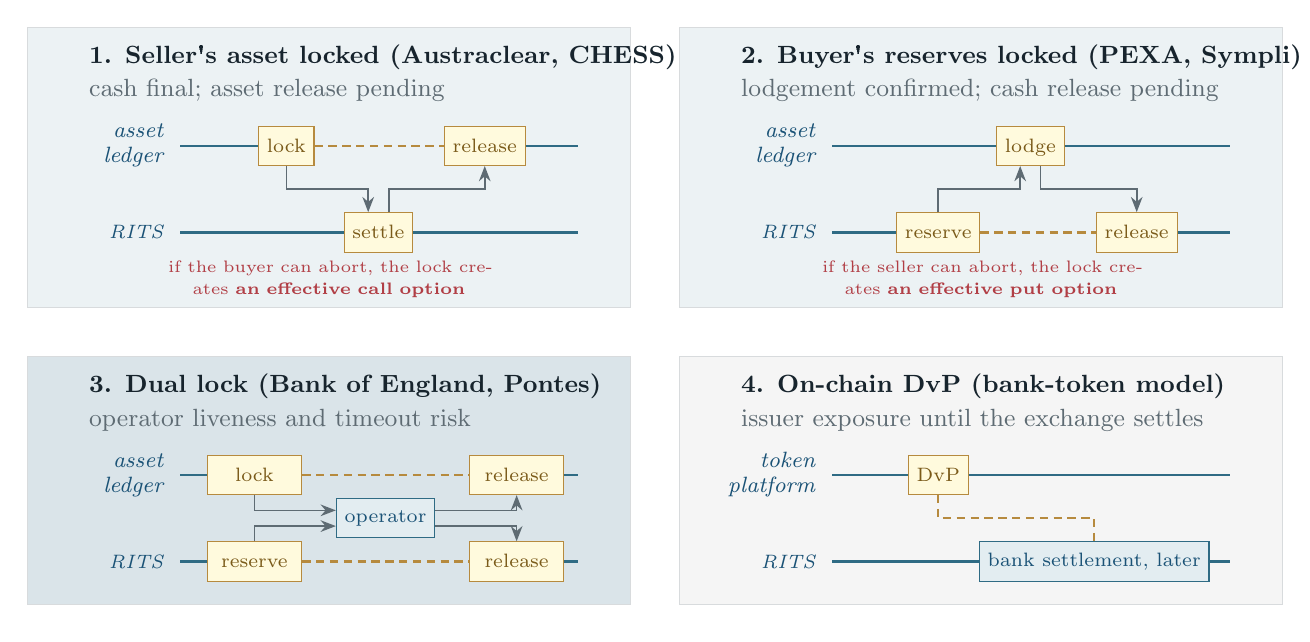
\begin{tikzpicture}[x=.90cm,y=1cm,ctl/.append style={-{Stealth[length=5.5pt,width=4.2pt]}},wl/.append style={text=Rust},ttl/.append style={font=\fontsize{9.4}{11.2}\selectfont\bfseries},bx/.append style={draw=defline,fill=deffill,text=deftext,text height=1.38ex,text depth=.30ex},hx/.append style={draw=lockline,fill=lockfill,text=locktext}]
% Equal 0.63 cm panel gutters in both directions.
\useasboundingbox (-1.85,3.05) rectangle (15.85,-4.40);
% Two-line ledger labels centred beside their wire.
\begin{scope}[shift={(-.30,0)}]
\node[ttl] at (-0.82,2.68) {1. Seller\textquotesingle s asset locked (Austraclear, CHESS)};
\node[nt,anchor=west,align=left,text width=7.2cm,font=\fontsize{9.2}{10.6}\selectfont] at (-0.82,2.25) {cash final; asset release pending};
\begin{scope}[yshift=-.05cm]
\node[wl,align=right,font=\fontsize{7.6}{9}\selectfont\itshape] at (0.5,1.6) {asset\\ledger}; \node[wl] at (0.5,0.5) {RITS};
\node[bx] (l1) at (2.1,1.6) {lock}; \node[bx] (r1) at (4.9,1.6) {release}; \node[bx] (s1) at (3.4,0.5) {settle};
\draw[wire] (0.6,1.6) -- (l1.west); \draw[held] (l1.east) -- (r1.west); \draw[wire] (r1.east) -- (6.22,1.6);
\draw[wire] (0.6,0.5) -- (s1.west); \draw[wire] (s1.east) -- (6.22,0.5);
% Lock confirmation enables cash settlement; settlement then enables asset release.
\draw[ctl] (l1.south) -- (2.1,1.05) -| ([xshift=-.13cm]s1.north);
\draw[ctl] ([xshift=.13cm]s1.north) |- (4.9,1.05) -- (r1.south);
\end{scope}
\node[nt,anchor=center,align=center,text width=7.05cm,text=RegulationRed,font=\fontsize{6.5}{7.8}\selectfont,inner sep=0pt] at (2.70,-.15) {if the buyer can abort, the lock creates \textbf{an effective call option}};
\end{scope}
\begin{scope}[shift={(8.90,0)}]
\node[ttl] at (-0.82,2.68) {2. Buyer\textquotesingle s reserves locked (PEXA, Sympli)};
\node[nt,anchor=west,align=left,text width=7.2cm,font=\fontsize{9.2}{10.6}\selectfont] at (-0.82,2.25) {lodgement confirmed; cash release pending};
\begin{scope}[yshift=-.05cm]
\node[wl,align=right,font=\fontsize{7.6}{9}\selectfont\itshape] at (0.5,1.6) {asset\\ledger}; \node[wl] at (0.5,0.5) {RITS};
\node[bx] (d2) at (3.4,1.6) {lodge}; \node[bx] (v2) at (2.1,0.5) {reserve}; \node[bx] (r2) at (4.9,0.5) {release};
\draw[wire] (0.6,1.6) -- (d2.west); \draw[wire] (d2.east) -- (6.22,1.6);
\draw[wire] (0.6,0.5) -- (v2.west); \draw[held] (v2.east) -- (r2.west); \draw[wire] (r2.east) -- (6.22,0.5);
% The reservation enables asset processing; its confirmation enables cash release.
\draw[ctl] (v2.north) -- (2.1,1.05) -| ([xshift=-.13cm]d2.south);
\draw[ctl] ([xshift=.13cm]d2.south) |- (4.9,1.05) -- (r2.north);
\end{scope}
\node[nt,anchor=center,align=center,text width=7.05cm,text=RegulationRed,font=\fontsize{6.5}{7.8}\selectfont,inner sep=0pt] at (2.70,-.15) {if the seller can abort, the lock creates \textbf{an effective put option}};
\end{scope}
\begin{scope}[shift={(-.30,-4.18)}]
\node[ttl] at (-0.82,2.68) {3. Dual lock (Bank of England, Pontes)};
\node[nt,anchor=west,align=left,text width=7.2cm,font=\fontsize{9.2}{10.6}\selectfont] at (-0.82,2.25) {operator liveness and timeout risk};
\begin{scope}[yshift=-.05cm]
\node[wl,align=right,font=\fontsize{7.6}{9}\selectfont\itshape] at (0.5,1.6) {asset\\ledger}; \node[wl] at (0.5,0.5) {RITS};
\node[bx,minimum width=1.2cm] (l3) at (1.65,1.6) {lock}; \node[bx,minimum width=1.2cm] (ra) at (5.35,1.6) {release};
\node[bx,minimum width=1.2cm] (v3) at (1.65,0.5) {reserve}; \node[bx,minimum width=1.2cm] (rb) at (5.35,0.5) {release};
\node[hx] (op) at (3.5,1.05) {operator};
\draw[wire] (0.6,1.6) -- (l3.west); \draw[held] (l3.east) -- (ra.west); \draw[wire] (ra.east) -- (6.22,1.6);
\draw[wire] (0.6,0.5) -- (v3.west); \draw[held] (v3.east) -- (rb.west); \draw[wire] (rb.east) -- (6.22,0.5);
% Equal spacing and mirrored right-angle control paths.
\draw[ctl] (l3.south) |- ([yshift=.1cm]op.west);
\draw[ctl] (v3.north) |- ([yshift=-.1cm]op.west);
\draw[ctl] ([yshift=.1cm]op.east) -| (ra.south);
\draw[ctl] ([yshift=-.1cm]op.east) -| (rb.north);
\end{scope}
\end{scope}
\begin{scope}[shift={(8.90,-4.18)}]
\node[ttl] at (-0.82,2.68) {4. On-chain DvP (bank-token model)};
\node[nt,anchor=west,align=left,text width=7.2cm,font=\fontsize{9.2}{10.6}\selectfont] at (-0.82,2.25) {issuer exposure until the exchange settles};
\begin{scope}[yshift=-.05cm]
\node[wl,align=right,font=\fontsize{7.6}{9}\selectfont\itshape] at (0.5,1.6) {token\\platform}; \node[wl] at (0.5,0.5) {RITS};
\node[bx,align=center] (dv) at (2.1,1.6) {DvP}; \node[hx] (nx) at (4.3,0.5) {bank settlement, later};
\draw[wire] (0.6,1.6) -- (dv.west); \draw[wire] (dv.east) -- (6.22,1.6);
\draw[wire] (0.6,0.5) -- (nx.west); \draw[wire] (nx.east) -- (6.22,0.5);
\draw[held] (dv.south) -- (2.1,1.05) -| (nx.north);
\end{scope}
\end{scope}
\begin{scope}[on background layer,overlay]
\filldraw[fill=Ocean!9!Paper,draw=Quiet!24!Paper,line width=.35pt] (-1.85,3.05) rectangle (6.65,-.50);
\filldraw[fill=Ocean!9!Paper,draw=Quiet!24!Paper,line width=.35pt] (7.35,3.05) rectangle (15.85,-.50);
\filldraw[fill=Ocean!18!Paper,draw=Quiet!24!Paper,line width=.35pt] (-1.85,-1.13) rectangle (6.65,-4.28);
\filldraw[fill=black!4!Paper,draw=Quiet!24!Paper,line width=.35pt] (7.35,-1.13) rectangle (15.85,-4.28);
\end{scope}
\end{tikzpicture}}
\end{center}
\vspace{-.12cm}

\end{frame}




% BEGIN central-bank-synchronisation.tex -- DO NOT SPLICE: hand-edited in place since generation; the source file on disk is stale
\begin{frame}[t]{Central bank synchronisation}
\hyphenpenalty=10000\exhyphenpenalty=10000
\vspace{.04cm}
\colorlet{StandardLinkText}{Ink!82!Paper}
\begin{tikzpicture}[
 smallcard/.style={draw=none,fill=none,text=StandardLinkText,anchor=north west,inner sep=0pt,text width=4.04cm,minimum height=.50cm,align=left,execute at begin node={\raggedright\hypersetup{urlcolor=StandardLinkText}},font=\fontsize{6.2}{7.5}\selectfont},
 bigcard/.style={draw=none,fill=none,anchor=north west,inner sep=.30cm,text width=6.32cm,align=left,font=\fontsize{7.3}{8.8}\selectfont}]
\begin{scope}[yshift=-4.23cm]
\fill[black!6!Paper] (0,-.045) rectangle (8.90,-2.64);
\node[anchor=center,inner sep=0pt,text=Rust,font=\fontsize{7.3}{8.8}\selectfont\bfseries] at (4.45,-.36) {RTGS-FMI links};
\node[smallcard] at (0.30,-0.45) {\href{https://www.rba.gov.au/payments-and-infrastructure/tokenised-money/the-role-of-rits-in-supporting-settlement-in-a-tokenised-ecosystem/overview-of-current-rits-and-fss-functionality.html}{\mbox{\flag{australia}~\textbf{Austraclear / CHESS}}}\newline\hspace*{1.45em}Securities--RITS links and batches};
\node[smallcard] at (4.56,-0.45) {\href{https://www.boj.or.jp/en/about/education/oshiete/kess/i17.htm}{\mbox{\flag{japan}~\textbf{BOJ-NET}}}\newline\hspace*{1.45em}JGB delivery-versus-payment; CSD links};
\node[smallcard] at (0.30,-1.09) {\href{https://www.frbservices.org/financial-services/securities}{\mbox{\flag{united-states}~\textbf{Fedwire Securities}}}\newline\hspace*{1.45em}Integrated securities--cash settlement};
\node[smallcard] at (4.56,-1.09) {\href{https://www.ecb.europa.eu/paym/target/t2s/html/index.en.html}{\mbox{\flag{eu}~\textbf{T2S}}}\newline\hspace*{1.45em}Common securities--cash platform};
\node[smallcard] at (0.30,-1.73) {\href{https://www.bankofengland.co.uk/payments/rtgs-future-roadmap}{\mbox{\flag{united-kingdom}~\textbf{CREST / RT2}}}\newline\hspace*{1.45em}CREST cycles; earmarked sterling cash};
\node[smallcard] at (4.56,-1.73) {\href{https://www.six-group.com/dam/download/securities-services/securities-finance/info-center/edu/srp-trading-theory-en.pdf}{\mbox{\flag{switzerland}~\textbf{SECOM / SIC}}}\newline\hspace*{1.45em}Linked securities--cash settlement};
\fill[black!6!Paper] (9.20,-.045) rectangle (14.74,-2.64);
\node[anchor=center,inner sep=0pt,text=Rust,font=\fontsize{7.3}{8.8}\selectfont\bfseries] at (11.97,-.36) {CLS multicurrency PvP};
\node[anchor=north west,inner sep=0pt,text=StandardLinkText,text width=4.94cm,align=left,execute at begin node={\hypersetup{urlcolor=StandardLinkText}},font=\fontsize{6.6}{8.2}\selectfont] at (9.50,-.56) {\href{https://www.cls-group.com/media/lnocyvna/cls_fna_report_reimagining_-sameday_fx_mar2025.pdf}{\mbox{\flag{international}~\textbf{Continuous Linked Settlement}}\newline 75-member user-owned utility created by the international banking industry in 2002. Enables PvP settlement across 18 currencies (over US\$8tn daily) within a five-hour window of overlapping RTGS hours (European morning).}};
\end{scope}
\begin{scope}[yshift=2.67cm]
\fill[SyncPanelBlueGrey,opacity=.16] (0,-2.62) rectangle (14.74,-6.68);
\node[anchor=center,inner sep=0pt,text=Rust,font=\displayfont\fontsize{10.5}{12.5}\selectfont\bfseries] at (7.37,-3.04) {Synchronisation Operator};
% Fixed backgrounds and top-aligned contents keep both flag/title rows level.
\fill[SyncPanelBlueGrey,opacity=.30] (.30,-3.42) rectangle (7.22,-6.55);
\fill[SyncPanelBlueGrey,opacity=.30] (7.52,-3.42) rectangle (14.44,-6.55);
\node[bigcard] at (.30,-3.42) {{\fontsize{8.1}{9.7}\selectfont\color{Rust}\href{https://www.bankofengland.co.uk/payments/rtgs-future-roadmap/what-is-synchro}{\mbox{\flag{united-kingdom}~\textcolor{Ink}{\textbf{Synchronisation Lab}}}}\hfill{\fontsize{6.6}{8.0}\selectfont\href{https://www.bankofengland.co.uk/news/2026/may/fca-and-boe-set-out-shared-vision-for-tokenisation-in-uk-wholesale-markets}{Target: 2028}}\par}
\vspace{.08cm}
{\fontsize{6.4}{7.7}\selectfont
\textcolor{black}{\textbf{Operator earmark and release.}} A \textbf{synchronisation operator} instructs \textbf{RT2} to earmark the payer's funds and the asset ledger to lock the asset. When both confirm, it instructs both to complete; if either fails the holds are released. Funds move between the participants' own RT2 accounts; the operator holds no central bank money. Intended uses include securities, FX and housing. Prototyped in \href{https://www.bis.org/publications/project-meridian-innovating-transactions-synchronisation}{\textbf{\mbox{Meridian (2023)}}} and \href{https://www.bis.org/project/meridian-fx}{\textbf{\mbox{Meridian FX (2025)}}}. A \href{https://www.bankofengland.co.uk/payments/rtgs-future-roadmap/synchronisation}{Synchronisation Lab} opens in 2026 for prospective operators.\par}};
\node[bigcard] at (7.52,-3.42) {{\fontsize{8.1}{9.7}\selectfont\color{Rust}\href{https://www.ecb.europa.eu/paym/target/pontes/html/index.en.html}{\mbox{\flag{eu}~\textcolor{Ink}{\textbf{Eurosystem Pontes}}}}\hfill{\fontsize{6.6}{8.0}\selectfont Launched: Sep 2026}\par}
\vspace{.08cm}
{\fontsize{6.4}{7.7}\selectfont
\textcolor{black}{\textbf{Assets on interoperable ledgers,}} \href{https://www.ecb.europa.eu/press/pr/date/2026/html/ecb.pr260921~e754847a7b.en.html}{with launch operators \textbf{Clearstream}, \textbf{SWIAT}, \textbf{Cashlink} and \textbf{Axiology}}. Connection through \textbf{Hash-Link}: the asset settles on their ledger and the cash leg is a direct T2 payment. The second route is a Eurosystem DLT cash-token platform (not yet live). \textbf{Pythagore}'s \href{https://www.banque-france.fr/en/monetary-strategy/markets/neu-cp-neu-mtn}{Negotiable EUropean Commercial Paper (NEU CP)} market is the first planned user, from end-2026. DLT tokenised reserves mirror T2 cash (the euro RTGS).\par}};
\end{scope}
\end{tikzpicture}\par
\end{frame}

% END central-bank-synchronisation.tex -- DO NOT SPLICE


% BEGIN central-bank-hours.tex -- DO NOT SPLICE: hand-edited in place since generation; the source file on disk is stale
\begin{frame}[t]{RTGS wholesale operating hours}
\newcommand{\retailstar}{{\fontsize{8}{8}\selectfont\bfseries\upshape *}}
\definecolor{CLSMagenta}{HTML}{FF00CC}
\definecolor{HoursYellow}{HTML}{FFF6C9}
\definecolor{RetailPurple}{HTML}{4B2266}
\definecolor{GridBlue}{HTML}{BFD6E8}
\colorlet{CoreTeal}{Ocean!82!Paper}
\hyphenpenalty=10000\exhyphenpenalty=10000
\vspace{.02cm}
\begin{tikzpicture}[x=1cm,y=.84cm,
  sys/.style={anchor=east,inner sep=0pt,font=\fontsize{8.1}{9.5}\selectfont\bfseries,text=Ink},
  zone/.style={anchor=west,inner sep=0pt,font=\fontsize{6.6}{7.8}\selectfont,text=Quiet},
  hours/.style={anchor=east,yshift=-1.1pt,inner sep=0pt,font=\fontsize{6.6}{7.8}\selectfont,text=Quiet},
  detail/.style={anchor=north west,inner sep=0pt,font=\fontsize{6.5}{7.5}\selectfont,text=Quiet},
  cash/.style={anchor=west,align=left,inner sep=0pt,font=\fontsize{5.3}{6.5}\selectfont\itshape,text=RetailPurple,execute at begin node={\hypersetup{urlcolor=RetailPurple,linkcolor=RetailPurple}}},
  tick/.style={anchor=south,inner sep=0pt,font=\fontsize{8.0}{9.2}\selectfont\bfseries,text=Quiet}]
\path[use as bounding box] (0,-7.24) rectangle (14.76,1.18);
\begin{scope}[xshift=.17cm]
% Shared 00--24 scale: x = 2.4 + 0.375 * local hour.
\fill[CoreTeal] (2.4,0.8800) rectangle (2.7,1.0500);
\node[zone] at (2.7937,.96) {Full / core};
\fill[HoursYellow] (4.275,0.8800) rectangle (4.575,1.0500);
\node[zone] at (4.6687,.96) {Restricted / optional};
\fill[BoxGrey!85!Quiet] (7.275,0.8800) rectangle (7.575,1.0500);
\node[zone] at (7.6687,.96) {Closed};
\fill[CLSMagenta] (9.0094,0.9500) rectangle (9.3094,1.0400);
\node[zone] at (9.4031,.96) {CLS pay-ins};
\node[sys,anchor=west,text=RetailPurple,font=\fontsize{6.4}{7.5}\selectfont\bfseries\itshape] at (12.01,.60) {24/7 retail};
\begin{scope}[yshift=-.12cm]
\foreach \h in {0,...,24} {\draw[GridBlue,line width=.4pt] ({2.4+.375*\h},.46)--({2.4+.375*\h},-6.16);}
\foreach \h in {0,3,6,9,12,15,18,21,24} {
  \node[tick,anchor=north,text=Rust] at ({2.4+.375*\h},-6.22) {\ifnum\h<10 0\fi\h:00};
  \node[tick,text=Rust] at ({2.4+.375*\h},.56) {\ifnum\h<10 0\fi\h:00};
}
\node[tick,anchor=north,font=\fontsize{8.4}{9.6}\selectfont] at (6.9,-6.86) {Local weekday hours};
\node[cash,anchor=north west,text width=2.18cm,font=\fontsize{5.3}{6.5}\selectfont] at (12.29,-6.14) {\retailstar\,Fast customer transfers with deferred interbank settlement};
\draw[Mist,line width=.3pt] (11.58,.97)--(11.58,-6.34);
% A little inner padding above the first bar and below the last.
\begin{scope}[shift={(0,-.12)},yscale=.957142857]
\foreach \y/\rowgap in {0/4,-.70/3,-1.40/2,-2.10/1,-2.80/0,-3.50/-1,-4.20/-2,-4.90/-3,-5.60/-4} {
  \begin{scope}[yshift=\rowgap pt]
  \fill[BoxGrey!85!Quiet,rounded corners=1.3pt] (2.4,{\y-.09}) rectangle (11.4,{\y+.09});
  \end{scope}
}
\begin{scope}[shift={(0,3.50)},yshift=4pt]
% SIC customer, bank and liquidity windows.
\node[sys] at (2.15,-3.36) {\href{https://www.snb.ch/public/asset/en/www-snb-ch/publications/sicsystem-disclosure/sicsystem-disclosure-all/sicsystem_disclosure_2024/publications0_en/sicsystem_disclosure_2024.en.pdf}{SIC RTGS~\flag{switzerland}}};
\begin{scope}\clip[rounded corners=1.3pt] (2.4,-3.5900) rectangle (11.4,-3.4100);\fill[CoreTeal] (2.4,-3.5900) rectangle (8.775,-3.4100);\end{scope}
\begin{scope}\clip[rounded corners=1.3pt] (2.4,-3.5900) rectangle (11.4,-3.4100);\fill[HoursYellow] (8.775,-3.5900) rectangle (9.2438,-3.4100);\end{scope}
\begin{scope}\clip[rounded corners=1.3pt] (2.4,-3.5900) rectangle (11.4,-3.4100);\fill[CoreTeal] (9.4313,-3.5900) rectangle (11.4,-3.4100);\end{scope}
\node[hours] at (2.15,-3.69) {Zurich};
\node[cash] at (12.01,-3.5) {\href{https://www.snb.ch/en/publications/communication/press-releases/2024/pre_20240821}{SIC instant (2024)}};
% CLS pay-ins, local time on 22 September 2026: 07:00--12:00.
\fill[CLSMagenta] (5.025,-3.7200) rectangle (6.9,-3.6300);
\end{scope}
\begin{scope}[shift={(0,1.40)},yshift=3pt]
% T2: ancillary-system/liquidity period outside the payment window.
\node[sys] at (2.15,-1.96) {\href{https://www.ecb.europa.eu/paym/target/shared/pdf/TARGET_System_operating_schedule.en.pdf}{T2~\flag{eu}}};
\begin{scope}\clip[rounded corners=1.3pt] (2.4,-2.1900) rectangle (11.4,-2.0100);\fill[HoursYellow] (2.4,-2.1900) rectangle (9.15,-2.0100);\end{scope}
\begin{scope}\clip[rounded corners=1.3pt] (2.4,-2.1900) rectangle (11.4,-2.0100);\fill[HoursYellow] (9.7125,-2.1900) rectangle (11.4,-2.0100);\end{scope}
\begin{scope}\clip[rounded corners=1.3pt] (2.4,-2.1900) rectangle (11.4,-2.0100);\fill[CoreTeal] (3.3375,-2.1900) rectangle (8.775,-2.0100);\end{scope}
\draw[Paper,dash pattern=on 1pt off 1pt,line width=.65pt] (3.525,-2.22) rectangle (4.275,-1.98);
\node[hours] at (2.15,-2.29) {Frankfurt};
\node[cash] at (12.01,-2.1) {\href{https://www.ecb.europa.eu/press/pr/date/2018/html/ecb.pr181130.en.html}{TIPS (2018)}};
% CLS pay-ins, local time on 22 September 2026: 07:00--12:00.
\fill[CLSMagenta] (5.025,-2.3200) rectangle (6.9,-2.2300);
\end{scope}
\begin{scope}[shift={(0,0.00)},yshift=2pt]
% Fedwire wraps across midnight; customer cutoff precedes bank cutoff.
\node[sys] at (2.15,-1.2600) {\href{https://www.frbservices.org/resources/financial-services/wires/operating-hours.html}{Fedwire~\flag{united-states}}};
\begin{scope}\clip[rounded corners=1.3pt] (2.4,-1.4900) rectangle (11.4,-1.3100);\fill[CoreTeal] (2.4,-1.4900) rectangle (9.4313,-1.3100);\end{scope}
\begin{scope}\clip[rounded corners=1.3pt] (2.4,-1.4900) rectangle (11.4,-1.3100);\fill[HoursYellow] (9.4313,-1.4900) rectangle (9.525,-1.3100);\end{scope}
\begin{scope}\clip[rounded corners=1.3pt] (2.4,-1.4900) rectangle (11.4,-1.3100);\fill[CoreTeal] (10.275,-1.4900) rectangle (11.4,-1.3100);\end{scope}
\node[hours] at (2.15,-1.5900) {New York};
\node[cash] at (12.01,-1.4000) {\href{https://www.federalreserve.gov/paymentsystems/fednow_about.htm}{FedNow (2023)} / \href{https://www.theclearinghouse.org/about/history}{RTP (2017)}};
% CLS pay-ins, local time on 22 September 2026: 01:00--06:00.
\fill[CLSMagenta] (2.775,-1.6200) rectangle (4.65,-1.5300);
\end{scope}
\begin{scope}[shift={(0,-1.40)},yshift=1pt]
% Lynx Rule 2: 00:30--18:00 window 1; 18:00--18:30 bank/return messages.
% Rule 3: optional early participation; all participants available from 08:00.
% Rule 6: before 06:00, CLS-related or bilaterally agreed payments only.
\node[sys] at (2.15,-0.5600) {\href{https://www.payments.ca/sites/default/files/rule_2_general.pdf}{Lynx~\flag{canada}}};
\begin{scope}\clip[rounded corners=1.3pt] (2.4,-0.7900) rectangle (11.4,-0.6100);\fill[HoursYellow] (2.5875,-0.7900) rectangle (9.3375,-0.6100);\end{scope}
\begin{scope}\clip[rounded corners=1.3pt] (2.4,-0.7900) rectangle (11.4,-0.6100);\fill[CoreTeal] (5.4,-0.7900) rectangle (9.15,-0.6100);\end{scope}
\node[hours] at (2.15,-0.8900) {Toronto};
\node[cash] at (12.01,-0.7000) {\href{https://www.interac.ca/en/company/about/our-history/}{Interac e-Transfer (2003)}\raisebox{.15ex}{\retailstar}};
% CLS CAD pay-ins: 01:00--06:00 Toronto on 22 September 2026.
\fill[CLSMagenta] (2.775,-0.9200) rectangle (4.65,-0.8300);
\end{scope}
\begin{scope}[shift={(0,-2.80)}]
% RITS: core daily session; other sessions restrict eligible transactions.
\node[sys] at (2.15,0.14) {\href{https://www.rba.gov.au/payments-and-infrastructure/rits/business-hours.html}{RITS~\flag{australia}}};
\begin{scope}\clip[rounded corners=1.3pt] (2.4,-0.0900) rectangle (11.4,0.0900);\fill[HoursYellow] (5.2125,-0.0900) rectangle (10.65,0.0900);\end{scope}
\begin{scope}\clip[rounded corners=1.3pt] (2.4,-0.0900) rectangle (11.4,0.0900);\fill[CoreTeal] (5.8688,-0.0900) rectangle (8.5875,0.0900);\end{scope}
\node[hours] at (2.15,-0.19) {Sydney};
\node[cash] at (12.01,0) {\href{https://www.rba.gov.au/media-releases/2018/mr-18-02.html}{NPP (2018)}};
% CLS pay-ins, local time on 22 September 2026: 15:00--18:00.
\fill[CLSMagenta] (8.025,-0.2200) rectangle (9.15,-0.1300);
\end{scope}
\begin{scope}[shift={(0,0.70)},yshift=-1pt]
% BOJ-NET optional access; month-end early opening is noted below.
\node[sys] at (2.15,-4.06) {\href{https://www.boj.or.jp/en/research/brp/psr/data/psr160624.pdf}{BOJ-NET~\flag{japan}}};
\begin{scope}\clip[rounded corners=1.3pt] (2.4,-4.2900) rectangle (11.4,-4.1100);\fill[HoursYellow] (5.5875,-4.2900) rectangle (10.275,-4.1100);\end{scope}
\begin{scope}\clip[rounded corners=1.3pt] (2.4,-4.2900) rectangle (11.4,-4.1100);\fill[CoreTeal] (5.775,-4.2900) rectangle (8.775,-4.1100);\end{scope}
\node[hours] at (2.15,-4.39) {Tokyo};
\node[cash] at (12.01,-4.2) {\href{https://www.zengin-net.jp/en/zengin_net/pdf/zengin-e.pdf}{Zengin More Time (2018)}\raisebox{.15ex}{\retailstar}};
% CLS pay-ins, local time on 22 September 2026: 14:00--17:00.
\fill[CLSMagenta] (7.65,-4.4200) rectangle (8.775,-4.3300);
\end{scope}
\begin{scope}[shift={(0,-1.40)},yshift=-2pt]
% CHAPS: current window plus announced optional early-morning extension, planned September 2027.
\node[sys] at (2.15,-2.66) {\href{https://www.bankofengland.co.uk/payments/faqs}{RT2 / CHAPS~\flag{united-kingdom}}};
\begin{scope}\clip[rounded corners=1.3pt] (2.4,-2.8900) rectangle (11.4,-2.7100);\fill[CoreTeal] (4.65,-2.8900) rectangle (9.025,-2.7100);\end{scope}
\begin{scope}\clip[rounded corners=1.3pt] (2.4,-2.8900) rectangle (11.4,-2.7100);\fill[HoursYellow] (9.025,-2.8900) rectangle (9.15,-2.7100);\end{scope}
\node[hours] at (2.15,-2.99) {London};
\node[cash] at (12.01,-2.8) {\href{https://www.wearepay.uk/who-we-are/heritage/}{Faster Payments (2008)}\raisebox{.15ex}{\retailstar}};
% CLS pay-ins, local time on 22 September 2026: 06:00--11:00.
\fill[CLSMagenta] (4.65,-3.0200) rectangle (6.525,-2.9300);
\end{scope}
\begin{scope}[shift={(0,0.00)},yshift=-3pt]
% BOK-Wire+ extended operating day introduced 30 March 2026.
\node[sys] at (2.15,-4.76) {\href{https://www.bok.or.kr/portal/bbs/B0000502/view.do?menuNo=201265\&nttId=10097174}{BOK-Wire+~\flag{south-korea}}};
\begin{scope}\clip[rounded corners=1.3pt] (2.4,-4.9900) rectangle (11.4,-4.8100);\fill[CoreTeal] (5.775,-4.9900) rectangle (9.9,-4.8100);\end{scope}
\node[hours] at (2.15,-5.09) {Seoul};
\node[cash] at (12.01,-4.9) {\href{https://www.bis.org/publications/quest-speed-payments}{KFTC EBS (2001)}\raisebox{.15ex}{\retailstar}};
% CLS pay-ins, local time on 22 September 2026: 14:00--17:00.
\fill[CLSMagenta] (7.65,-5.1200) rectangle (8.775,-5.0300);
\end{scope}
\begin{scope}[shift={(0,0.00)},yshift=-4pt]
% HKD CHATS: customer cutoff 18:00, bank cutoff 18:30; CLS pay-ins 13:00--16:00.
\node[sys] at (2.15,-5.46) {\href{https://www.hkma.gov.hk/media/eng/doc/key-functions/financial-infrastructure/infrastructure/HKD_CHATS_DF.pdf}{HKD CHATS~\flag{hong-kong}}};
\begin{scope}\clip[rounded corners=1.3pt] (2.4,-5.6900) rectangle (11.4,-5.5100);\fill[CoreTeal] (5.5875,-5.6900) rectangle (9.15,-5.5100);\end{scope}
\begin{scope}\clip[rounded corners=1.3pt] (2.4,-5.6900) rectangle (11.4,-5.5100);\fill[HoursYellow] (9.15,-5.6900) rectangle (9.3375,-5.5100);\end{scope}
\node[hours] at (2.15,-5.79) {Hong Kong};
\node[cash] at (12.01,-5.6) {\href{https://www.hkma.gov.hk/media/eng/publication-and-research/quarterly-bulletin/qb201809/fa2.pdf}{HKD FPS (2018)}};
\fill[CLSMagenta] (7.275,-5.8200) rectangle (8.4,-5.7300);
\end{scope}
\end{scope}
\end{scope}
\end{scope}
\end{tikzpicture}\par
\end{frame}

% END central-bank-hours.tex -- DO NOT SPLICE


% BEGIN synchronisation-requirements.tex -- DO NOT SPLICE: hand-edited in place since generation; the source file on disk is stale
\begin{frame}[t]{Synchronisation: RITS requirements}
\setbeamerfont{itemize/enumerate body}{size=\fontsize{8.0}{10.0}}\fontsize{8.0}{10.0}\selectfont
\vspace{-0.1em}
  {\color{Ink}\bfseries\fontsize{8.2}{10}\selectfont Shorter term\par}\vspace{-0.15em}
  \vspace{0pt plus 0.35fill}\begin{itemize}\setlength{\itemsep}{2pt plus 2.4fill}
    \item \rust{Reservation lock on the FSS.} Continuous \textbf{\textit{hold}}, \textbf{\textit{observe}} and \textbf{\textit{release}} functionality on the settlement account, as in the Eurosystem's \textbf{TIPS} (retail payment system). The FSS lacks this.
    \item \rust{API on RITS/FSS.} ISO 20022 already has reservation messages, \textbf{\texttt{camt.046}} to \textbf{\texttt{camt.049}}, used in the Eurosystem's \textbf{T2} and \textbf{T2S}. Operations \texttt{lock}, \texttt{status}, \texttt{settle} and \texttt{release}, with callbacks \texttt{accepted}, \texttt{expiring}, \texttt{settled} and \texttt{rejected}.
    \item \rust{Defined operator class.} Authority to instruct a hold on another party's reserves and trigger their release, assuming liability for erroneous release. PEXA and Sympli do this today without infrastructure status. \href{https://www.bankofengland.co.uk/minutes/2026/april/synchronisation-thematic-engagement-working-group}{The Bank of England is scoping this class with UK regulators.}
  \end{itemize}
\vspace{0.30cm plus 1fill}
  {\color{Ink}\bfseries\fontsize{8.2}{10}\selectfont Longer term\par}\vspace{-0.15em}
  \vspace{0pt plus 0.35fill}\begin{itemize}\setlength{\itemsep}{2pt plus 2.4fill}
    \item \rust{Intraday credit inside the settlement transaction.} T2S-style \textbf{auto-collateralisation against the asset being bought} using ISO~20022 messaging. Would require compatible collateral and securities-system interfaces.
    \item \rust{Admission rules.} RITS could synchronise with different types of operator, in some cases introducing financial stability risks. Formalised platform accreditation criteria must limit operator scope in line with \emph{PFMI} standards.
  \end{itemize}\vspace{0pt plus 1.2fill}
\vspace*{1.5pt}
\par\vspace{.15em}{\color{Rust!25!Paper}\hrule height .35pt}\vspace{.15em}
\defs{\fontsize{7.3}{8.8}\selectfont\color{Rust}\textbf{PayTo} does not supply a reservation, only authorisation to a payee to initiate a payment; the payer's bank then sends an ordinary NPP payment, which the FSS settles on receipt. Any hold is on the customer's account at the bank, not on ESA funds.}
\vspace*{\dimexpr1.1em+0.0858bp\relax}% Preserve the footnote bottom margin after increasing its type size.
\end{frame}

% END synchronisation-requirements.tex -- DO NOT SPLICE

% Recommendations are incorporated into Area 1 submission responses and requirements.


% BEGIN consultation-area-2.tex
{\setbeamercolor{background canvas}{bg=Rust}
\begin{frame}[plain]
\begin{tikzpicture}[remember picture,overlay]
% Whole block centred on the page: label and title centred, questions left-aligned (6 Oct 2026).
\node[anchor=center,inner sep=0pt] at (current page.center) {\begin{minipage}{13.40cm}\hyphenpenalty=10000\exhyphenpenalty=10000
{\centering{\color{Mist}\displayfont\fontsize{9}{11}\selectfont AREA 2\par}\vspace{.12cm}{\color{White}\displayfont\fontsize{22.5}{26.4}\selectfont\bfseries At-par exchange\par}}
\vspace{.95cm}{\raggedright\color{White}\fontsize{8.2}{10.4}\selectfont \textbf{Q5.} What exchange models (simple exchange, exchange with synchronisation, or DLT exchange) should RITS and/or the FSS be capable of supporting?\par\vspace{.42cm}\textbf{Q6.} For exchange models requiring synchronisation, what types of synchronisation arrangements (bilateral, third-party, central bank-supported or other) should be supported?\par\vspace{.42cm}\textbf{Q7.} To what extent do existing RITS and FSS capabilities and services enable the exchange models that are needed to support current and anticipated use cases?\par\vspace{.42cm}\textbf{Q8.} What enhancements to the existing services and capabilities are required to support exchange use cases that cannot be adequately supported using existing functionality?\par}
\end{minipage}};
\end{tikzpicture}
\end{frame}}

% User preference: no editorial gap or to-do footnotes on submission responses.


% END consultation-area-2.tex


\begin{frame}[t]{Par and tokenised money}
\setbeamerfont{itemize/enumerate body}{size=\fontsize{8.0}{10.0}}\fontsize{8.0}{10.0}\selectfont
\vspace{-0.1em}
  \vspace{0pt plus 0.35fill}\begin{itemize}\setlength{\itemsep}{2pt plus 2.4fill}
    \item \rust{Monetary singleness.} Australian money is primarily held as bank deposits. Payments between deposit accounts at different banks create interbank obligations that are settled, gross or net, by \textbf{transfers between banks' reserve accounts in RITS}. This requirement limits banks' deposit creation and ensures the \textbf{fungibility of AUD deposits} at different banks.
    \item \rust{Par under tokenisation.} A deposit token can circulate within one issuer\textquotesingle s liability. Cross-issuer par exchange needs redemption and settlement arrangements, liquidity and scheme rules. Retail holders ordinarily redeem into bank deposits; they do not hold ESAs.
    \item \rust{Project Acacia recommendation.} Bilateral convertibility becomes harder to scale as issuers and platforms multiply. A \textbf{multilateral mint-burn mechanism} linked to interbank settlement would make bank-issued deposit tokens fungible, as RITS ESA settlement does for bank deposits, supporting monetary singleness.
    \item \rust{Reserves-lock design.} Requires a hold on central bank funds to support \textbf{24/7 synchronisation}, or \textbf{tokenisation of reserves}. Preferable to designs that can only lock the token or asset on the external platform.
    \item \rust{Open questions.} \textit{If RITS supports exchange between deposit tokens, should it also support exchange between other regulated money tokens (stablecoins)? Should RITS enforce par value of legally distinct instruments? Which forms of tokenised private money should be eligible for exchange through RITS/FSS? What about a regulated industry ledger, privately operated under national scheme rules?}
  \end{itemize}\vspace{0pt plus 4fill}
\end{frame}

\begin{frame}{Interbank messaging and payments}
\vspace{-0.35em}
\begin{center}
\hyphenpenalty=10000 \exhyphenpenalty=10000 \adjustbox{max width=\textwidth,max height=4.05cm}{%
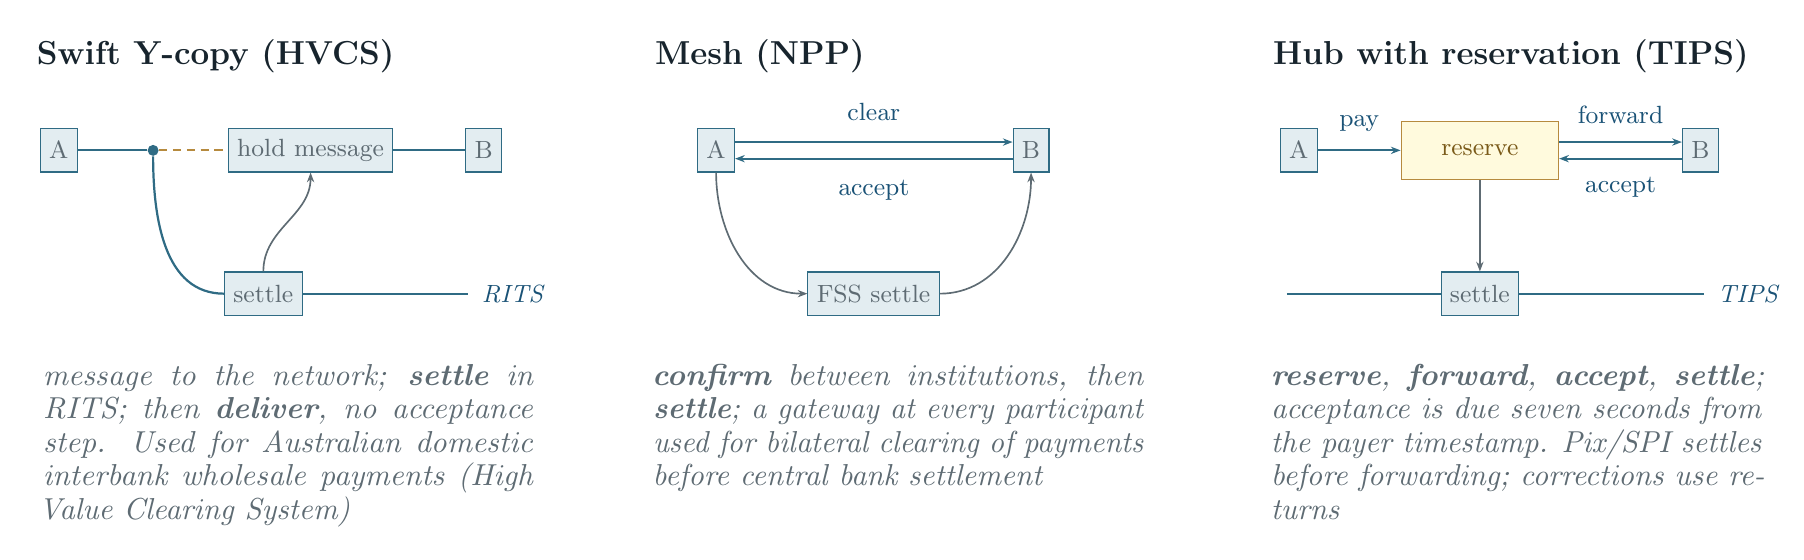
\begin{tikzpicture}[x=1cm,y=1.40cm,
 bx/.append style={text=Quiet,font=\fontsize{9.4}{11.0}\selectfont,minimum height=.55cm,inner sep=3.2pt},
 hx/.append style={font=\fontsize{9.4}{11.0}\selectfont,inner sep=3.2pt},
 wl/.append style={text=Rust,font=\fontsize{9.4}{11.0}\selectfont\itshape}]
% -Y-copy-
\begin{scope}[shift={(0,0)}]
\node[anchor=west,font=\large\bfseries,text=Ink] at (0,2.55) {Swift Y-copy (HVCS)};
\node[bx] (A0) at (0.4,1.7) {A};
\node[pt] (c) at (1.6,1.7) {};
\node[bx] (h) at (3.6,1.7) {hold message};
\draw[wire] (A0.east) -- (c); \draw[held] (c) -- (h.west); \node[bx] (B0) at (5.8,1.7) {B};
\draw[wire] (h.east) -- (B0.west);
\node[bx] (st) at (3.0,0.4) {settle};
\draw[wire] (c) to[out=270,in=180] (st.west); \draw[wire] (st.east) -- (5.6,0.4); \node[wl,anchor=west] at (5.65,0.4) {RITS};
\draw[ctl] (st.north) to[out=90,in=270] (h.south);
\node[nt,font=\fontsize{10.6}{12.1}\selectfont\itshape,text=Quiet,text width=6.2cm,align=justify,anchor=north west] at (0.10,-0.15) {message to the network; \textbf{settle} in RITS; then \textbf{deliver}, no acceptance step. Used for Australian domestic interbank wholesale payments (High Value Clearing System)};
\end{scope}
% -mesh-
\begin{scope}[shift={(7.85,0)}]
\node[anchor=west,font=\large\bfseries,text=Ink] at (0,2.55) {Mesh (NPP)};
\node[bx] (A) at (0.9,1.7) {A};
\node[bx] (B) at (4.9,1.7) {B};
\draw[wire,-{Stealth[length=3.5pt]}] ([yshift=3pt]A.east) -- node[above=4pt,font=\fontsize{9.4}{11.0}\selectfont,text=Rust] {clear} ([yshift=3pt]B.west);
\draw[wire,-{Stealth[length=3.5pt]}] ([yshift=-3pt]B.west) -- node[below=4pt,font=\fontsize{9.4}{11.0}\selectfont,text=Rust] {accept} ([yshift=-3pt]A.east);
\node[bx] (F) at (2.9,0.4) {FSS settle};
\draw[ctl] (A.south) to[out=270,in=180] (F.west);
\draw[ctl] (F.east) to[out=0,in=270] (B.south);
\node[nt,font=\fontsize{10.6}{12.1}\selectfont\itshape,text=Quiet,text width=6.2cm,align=justify,anchor=north west] at (0.00,-0.15) {\textbf{confirm} between institutions, then \textbf{settle}; a gateway at every participant used for bilateral clearing of payments before central bank settlement};
\end{scope}
% -hub with reservation-
\begin{scope}[shift={(15.70,0)}]
\node[anchor=west,font=\large\bfseries,text=Ink] at (0,2.55) {Hub with reservation (TIPS)};
\node[bx] (A2) at (0.45,1.7) {A};
\node[hx,minimum width=2.0cm,minimum height=0.74cm,align=center] (H) at (2.75,1.7) {reserve};
\node[bx] (S2) at (2.75,0.4) {settle};
\draw[wire] (0.3,0.4) -- (S2.west); \draw[wire] (S2.east) -- (5.6,0.4); \node[wl,anchor=west] at (5.65,0.4) {TIPS};
\draw[ctl] (H.south) -- (S2.north);
\node[bx] (B2) at (5.55,1.7) {B};
\draw[wire,-{Stealth[length=3.5pt]}] (A2.east) -- node[above=3pt,font=\fontsize{9.4}{11.0}\selectfont,text=Rust] {pay} (H.west);
\draw[wire,-{Stealth[length=3.5pt]}] ([yshift=3pt]H.east) -- node[above=3pt,font=\fontsize{9.4}{11.0}\selectfont,text=Rust] {forward} ([yshift=3pt]B2.west);
\draw[wire,-{Stealth[length=3.5pt]}] ([yshift=-3pt]B2.west) -- node[below=3pt,font=\fontsize{9.4}{11.0}\selectfont,text=Rust] {accept} ([yshift=-3pt]H.east);
\node[nt,font=\fontsize{10.6}{12.1}\selectfont\itshape,text=Quiet,text width=6.2cm,align=justify,anchor=north west] at (0.00,-0.15) {\textbf{reserve}, \textbf{forward}, \textbf{accept}, \textbf{settle}; acceptance is due seven seconds from the payer timestamp. Pix/SPI settles before forwarding; corrections use returns};
\end{scope}
% Retain the illustration's existing extent when italic captions occupy fewer lines.
\pgfresetboundingbox
\path[use as bounding box] (0.2pt,-70.0892pt) rectangle (631.7202pt,112.05133pt);
\end{tikzpicture}}
\end{center}
\vspace{0.15em}{\color{neutline}\hrule height 0.5pt}\vspace{\dimexpr0.35em+1.5pt\relax}
{\fontsize{7.0}{8.6}\selectfont\color{Rust}\hypersetup{urlcolor=Rust} \textbf{NPP Australia} contracted \textbf{Swift} to build and operate a \textbf{mesh of bilateral payment gateways (PAGs)} that clear payments between banks before they are settled in the FSS. An alternative to a mesh is a \textbf{hub model}, with clearing provided by a central facility like settlement.\\[1.2pt]Hub model examples include: \textbf{TIPS} and \textbf{RT1}~\scalebox{0.93}{\flag{eu}}, \textbf{FedNow} and \textbf{RTP}~\scalebox{0.93}{\flag{united-states}}, \textbf{Pix}~\scalebox{0.93}{\flag{brazil}}, \textbf{Faster Payments}~\scalebox{0.93}{\flag{united-kingdom}}, \textbf{Zengin}~\scalebox{0.93}{\flag{japan}}, \textbf{SIC instant}~\scalebox{0.93}{\flag{switzerland}}, \textbf{SPEI}~\scalebox{0.93}{\flag{mexico}}, \textbf{FPS}~\scalebox{0.93}{\flag{hong-kong}}, the \textbf{Real-Time Rail}~\scalebox{0.93}{\flag{canada}}, \textbf{UPI}~\scalebox{0.93}{\flag{india}}, \textbf{PayNow}~\scalebox{0.93}{\flag{singapore}}, \textbf{PromptPay}~\scalebox{0.93}{\flag{thailand}}, \textbf{DuitNow}~\scalebox{0.93}{\flag{malaysia}}, \textbf{BI-FAST}~\scalebox{0.93}{\flag{indonesia}} and \textbf{InstaPay}~\scalebox{0.93}{\flag{philippines}}.\par\vspace{1.5pt}{\fontsize{5.2}{6.2}\selectfont\noindent\resizebox{\linewidth}{!}{\textit{The last six are the members of \href{https://www.bis.org/about/bisih/topics/fmis/nexus.htm}{\textbf{Project Nexus}}, which will connect these national retail payment systems through a \textbf{cross border hub} for real-time cross-currency retail payments.}}\par}\smallskip \textbf{Australia is the only jurisdiction using a mesh infrastructure design for fast retail payments. This locks in ongoing vendor costs in the order of tens of millions annually. An enhanced FSS would be able to service the NPP under a more efficient hub design, retiring the legacy Swift PAG network.}\par}
\vspace{-1.5pt}
\end{frame}




\fi

\iftrue % Unhidden 6 Oct 2026 (was hidden 5 Oct 2026: Messaging and tokens, Money tokens, Par reachability for money tokens; kept in the source.
% BEGIN messages-vs-tokens.tex -- DO NOT SPLICE: hand-edited in place since generation; the source file on disk is stale
\begin{frame}[t]{Messaging and tokens}
\hyphenpenalty=10000\exhyphenpenalty=10000
\begin{tikzpicture}[remember picture,overlay,x=1cm,y=1cm,
 sectionhead/.style={anchor=north west,inner sep=0pt,text=Ink,font=\sffamily\fontsize{9.1}{10.9}\selectfont\bfseries},
 caption/.style={anchor=north west,inner sep=0pt,align=left,text=Quiet,font=\fontsize{6.3}{7.6}\selectfont\itshape},
 bank/.style={rectangle,draw=lockline,fill=lockfill,line width=.30pt,text=locktext,font=\fontsize{5.4}{6.5}\selectfont,minimum width=.92cm,minimum height=.35cm,inner xsep=2pt,inner ysep=1.2pt,outer sep=0pt},
 record/.style={bank,minimum width=1.18cm,minimum height=.51cm,align=center},
 flow/.style={draw=lockline,line width=.50pt,-{Stealth[length=3.8pt,width=3.0pt]}},
 update/.style={draw=Quiet,line width=.38pt,-{Stealth[length=3.8pt,width=3.0pt]}},
 smalllabel/.style={font=\fontsize{7.0}{8.3}\selectfont,text=Rust,inner sep=.7pt},
 owner/.style={record,minimum width=1.10cm,minimum height=.37cm},
 moneycard/.style={anchor=north west,inner xsep=.16cm,inner ysep=.13cm,text width=2.985cm,align=left,text=Ink,font=\fontsize{5.8}{6.4}\selectfont}]
\begin{scope}[shift={(current page.north west)}]
% Headings retain their order; the layers within each diagram are reversed.
\node[sectionhead] at (.83,-1.50) {Messages};
\node[caption,text width=6.40cm] at (.83,-1.94) {instruct a trusted intermediary to pay. Banks and the interbank settlement system (RITS) update separate ledgers.};
\begin{scope}[shift={(4.03,-3.50)},scale=.94,transform shape]
\node[record,draw=defline,fill=deffill,text=deftext,minimum width=1.40cm] (bookA) at (-2,.38) {Ledger A\\$-$100};
\node[record,draw=black!72,fill=black!72,text=white,minimum width=1.56cm,minimum height=.60cm,font=\fontsize{6.4}{7.6}\selectfont\bfseries] (reserve) at (0,.38) {RITS / ESAs\\settlement};
\node[record,draw=defline,fill=deffill,text=deftext,minimum width=1.40cm] (bookB) at (2,.38) {Ledger B\\$+$100};
\node[bank,font=\fontsize{6.4}{7.6}\selectfont] (messageA) at (-2,-.35) {\textbf{Bank A}};
\node[bank,font=\fontsize{6.4}{7.6}\selectfont] (messageB) at (2,-.35) {\textbf{Bank B}};
\draw[flow] (messageA.east) -- node[smalllabel,below=2pt] {payment message} (messageB.west);
\draw[update] (messageA.north) -- (bookA.south);
\draw[update] (0,-.35) -- (reserve.south);
\draw[update] (messageB.north) -- (bookB.south);
\end{scope}

\node[sectionhead] at (.83,-4.52) {Tokens};
\node[caption,text width=6.40cm] at (.83,-4.96) {Native tokens transfer the recorded claim on an authoritative shared ledger. Mirror and instruction tokens can still require external settlement. Finality depends on the legally authoritative record.};
\begin{scope}[shift={(4.03,-6.58)},scale=.94,transform shape]
\draw[draw=defline,fill=deffill,line width=.30pt] (-2.70,.42) rectangle (2.70,-.38);
\node[anchor=north,inner sep=0pt,text=Ink,font=\fontsize{7.0}{8.3}\selectfont] at (0,.35) {\textbf{Shared ledger}};
\node[owner,draw=neutline,fill=Paper,text=Quiet,dash pattern=on 1.5pt off 1.4pt] (ownerA) at (-2,-.02) {A: 100};
\node[owner,draw=defline,fill=deffill,text=deftext] (ownerB) at (2,-.02) {B: 100};
\node[bank,font=\fontsize{6.4}{7.6}\selectfont] (tokenA) at (-2,-.94) {\textbf{Bank A}};
\node[bank,font=\fontsize{6.4}{7.6}\selectfont] (tokenB) at (2,-.94) {\textbf{Bank B}};
\draw[flow] (ownerA.east) -- node[smalllabel,below=1.5pt] {native claim transfer} (ownerB.west);
\draw[update] (tokenA.north) -- (ownerA.south);
\draw[update] (ownerB.south) -- (tokenB.north);
\end{scope}

% Right-hand panel, reserved for the disintermediation material.
\filldraw[fill=DesignBlue,draw=Quiet!25,line width=.3pt] (7.91,-0.47) rectangle (15.38,-7.87);
\node[anchor=north west,inner sep=0pt,text width=7.03cm,align=justify,text=Ink,font=\fontsize{6.6}{7.9}\selectfont] at (8.13,-1.13) {A token can function as a \textbf{cryptographic bearer instrument}, a digital equivalent to physical cash (knowledge of secret keys as possession) which is held and transferred between \textbf{self-custodial} users without a bank's involvement. Like physical cash, it may be unrecoverable if lost.\par\vspace{1.5pt}A \textbf{retail CBDC} could circulate in this manner without settlement risk, likely reducing public demand for banking services. A \textbf{stablecoin} can also circulate in this manner, but is subject to credit and liquidity risk and its par value will depend on user acceptance.\\\textbf{Deposit token interchange} preserves the position of banks as token issuers: with tokens being burned and minted in transfer (with interbank settlement support) instead of circulating freely.\par};
% Two placeholders fill the lower half of the panel.
\filldraw[fill=Paper,draw=Quiet!30,line width=.3pt] (8.13,-4.47) rectangle (11.52,-7.65);
\filldraw[fill=Paper,draw=Quiet!30,line width=.3pt] (11.77,-4.47) rectangle (15.16,-7.65);
\node[anchor=north,inner sep=0pt,text=Quiet,font=\sffamily\fontsize{7.5}{9.0}\selectfont\bfseries] at (9.825,-4.59) {Bearer payments};
\node[anchor=north,inner sep=0pt,text=Quiet,font=\sffamily\fontsize{7.5}{9.0}\selectfont\bfseries] at (13.465,-4.59) {Bank payments};
% Three holders passing a token directly between themselves, no intermediary.
\begin{scope}[yshift=-.34cm,rotate around={60:(9.825,-5.815)}]
% Native macOS emoji glyphs; rendered from Apple Color Emoji.
\definecolor{FlowGreen}{HTML}{1F9250}
\draw[FlowGreen,line width=1.4pt,opacity=.85,-{Stealth[length=4.5pt,width=3.4pt]}] ([shift={(70:1.05)}]9.825,-5.815) arc[start angle=70,end angle=-10,radius=1.05];
\draw[FlowGreen,line width=1.4pt,opacity=.85,-{Stealth[length=4.5pt,width=3.4pt]}] ([shift={(-50:1.05)}]9.825,-5.815) arc[start angle=-50,end angle=-130,radius=1.05];
\draw[FlowGreen,line width=1.4pt,opacity=.85,-{Stealth[length=4.5pt,width=3.4pt]}] ([shift={(190:1.05)}]9.825,-5.815) arc[start angle=190,end angle=110,radius=1.05];
\node[inner sep=0pt] at (9.825,-4.765) {\includegraphics[width=0.74cm]{figures/emoji/apple-color/1f642.png}};
\node[inner sep=0pt] at (10.734,-6.340) {\includegraphics[width=0.74cm]{figures/emoji/apple-color/1f642.png}};
\node[inner sep=0pt] at (8.916,-6.340) {\includegraphics[width=0.74cm]{figures/emoji/apple-color/1f642.png}};
\foreach \coinangle in {30,-90,150} {
  \fill[Paper] ([shift={(\coinangle:1.05)}]9.825,-5.815) circle[radius=.212cm];
}
\node[inner sep=0pt] at ([shift={(30:1.05)}]9.825,-5.815) {\includegraphics[width=0.40cm]{figures/emoji/apple-color/1fa99.png}};
\node[inner sep=0pt] at ([shift={(-90:1.05)}]9.825,-5.815) {\includegraphics[width=0.40cm]{figures/emoji/apple-color/1fa99.png}};
\node[inner sep=0pt] at ([shift={(150:1.05)}]9.825,-5.815) {\includegraphics[width=0.40cm]{figures/emoji/apple-color/1fa99.png}};
\end{scope}
% Three banks exchange payments through a differently coloured central bank.
\begin{scope}[shift={(13.465,-5.985)}]
\foreach \fromangle/\toangle in {150/30,30/-90,-90/150} {
  \draw[Quiet,line width=.5pt,opacity=.65,dash pattern=on .35pt off 1.4pt,line cap=round,shorten <=.38cm,shorten >=.38cm,-{Stealth[length=2.6pt,width=2.0pt]}] (\fromangle:1.18) -- (\toangle:1.18);
}
\foreach \bankangle in {30,150,-90} {
  \begin{scope}[rotate=\bankangle]
    \draw[RegulationRed,line width=1.4pt,opacity=.85,-{Stealth[length=3.3pt,width=2.8pt]}] (.43,-.075) -- (.77,-.075);
    \draw[RegulationRed,line width=1.4pt,opacity=.85,-{Stealth[length=3.3pt,width=2.8pt]}] (.77,.075) -- (.43,.075);
  \end{scope}
}
\node[inner sep=0pt] (paybankA) at (150:1.18) {\includegraphics[width=.64cm]{figures/emoji/apple-color/1f3e6.png}};
\node[inner sep=0pt] (paybankB) at (30:1.18) {\includegraphics[width=.64cm]{figures/emoji/apple-color/1f3e6.png}};
\node[inner sep=0pt] (paybankC) at (-90:1.18) {\includegraphics[width=.64cm]{figures/emoji/apple-color/1f3e6.png}};
\node[inner sep=0pt] at (0,0) {\includegraphics[width=.68cm]{figures/emoji/apple-color/1f3e6-central.png}};
\node[inner sep=0pt] (payfaceA) at (-.928,-.298) {\includegraphics[width=.30cm]{figures/emoji/apple-color/1f610.png}};
\node[inner sep=0pt] (payfaceB) at (.207,.953) {\includegraphics[width=.30cm]{figures/emoji/apple-color/1f610.png}};
\node[inner sep=0pt] (payfaceC) at (.721,-.655) {\includegraphics[width=.30cm]{figures/emoji/apple-color/1f610.png}};
\definecolor{FlowGreen}{HTML}{1F9250}
\foreach \bankid in {A,B,C} {
  \draw[FlowGreen,line width=.45pt,shorten <=.025cm,shorten >=.025cm,-{Stealth[length=2.5pt,width=1.9pt]}] (payface\bankid) -- (paybank\bankid);
}
\end{scope}
\node[anchor=center,inner sep=0pt,text=Rust,font=\displayfont\fontsize{7.8}{9.3}\selectfont\bfseries] at (11.645,-0.79) {Disintermediation};
\draw[neutline,line width=.35pt] (.44,-8.02) -- (15.56,-8.02);
\node[anchor=north west,inner sep=0pt,text width=14.76cm,align=left,text=DeckBurgundy,font=\fontsize{6.0}{7.0}\selectfont] at (.62,-8.16) {\textbf{ISO 20022} (2004) standardises financial messages. \href{https://www.swift.com/standards/iso-20022/iso-20022-financial-institutions-focus-payments-instructions}{Swift's Cross-Border Payments and Reporting Plus (CBPR+) migration for payment instructions ran Mar-23 to Nov-25}, replacing earlier MT messages. \href{https://www.iso20022.org/contact-us}{Swift is its Registration Authority} and publishes the \href{https://www.iso20022.org/financial-repository}{ISO 20022 data dictionary and business-process catalogue}.};
\end{scope}
\end{tikzpicture}
\end{frame}

% END messages-vs-tokens.tex -- DO NOT SPLICE

% Money tokens, its own slide; cards run the full width, no enclosing panel.
\begin{frame}[t]{Money tokens}
\hyphenpenalty=10000\exhyphenpenalty=10000
\begin{tikzpicture}[remember picture,overlay,x=1cm,y=1cm,
 moneycard/.style={anchor=north west,inner sep=0pt,text width=9.35cm,align=justify,text=Ink,font=\fontsize{6.2}{7.4}\selectfont}]
\begin{scope}[shift={(current page.north west)}]
\filldraw[fill=black!6!Paper,draw=Quiet!25,line width=.3pt] (10.36,-1.05) rectangle (15.48,-7.86);
\node[anchor=center,inner sep=0pt,text=FootnoteBlue,font=\displayfont\fontsize{8.8}{10.5}\selectfont\bfseries] at (12.92,-1.37) {Money hierarchy};
% Four layers of the money hierarchy, highest claim at the top.
\filldraw[fill=black!6!Paper,draw=Quiet!55,dash pattern=on 1.1pt off 1.3pt,line width=.6pt] (10.9515,-1.755) rectangle (14.8885,-2.652);
\node[anchor=center,inner sep=0pt,align=center,text=Quiet,font=\sffamily\fontsize{7.2}{8.2}\selectfont] at (12.920,-2.2035) {\textbf{Gold/Forex}\\[1pt]{\fontsize{6.0}{6.8}\selectfont gold standard, fixed exchange rate}};
\filldraw[fill=DesignYellow,draw=Quiet!45,line width=1.0pt] (10.9515,-2.992) rectangle (14.8885,-3.889);
\node[anchor=center,inner sep=0pt,align=center,text=Ink,font=\sffamily\fontsize{7.2}{8.2}\selectfont] at (12.920,-3.4405) {\textbf{Central Bank Money}\\[1pt]{\fontsize{6.0}{6.8}\selectfont reserves, banknotes, CBDC}};
\filldraw[fill=DesignYellow!50!DesignBlue,draw=Quiet!45,line width=1.0pt] (10.9515,-4.229) rectangle (14.8885,-5.126);
\node[anchor=center,inner sep=0pt,align=center,text=Ink,font=\sffamily\fontsize{7.2}{8.2}\selectfont] at (12.920,-4.6775) {\textbf{Commercial Bank Money}\\[1pt]{\fontsize{6.0}{6.8}\selectfont deposits, tokenised deposits}};
\filldraw[fill=DesignBlue,draw=Quiet!45,line width=1.0pt] (10.9515,-5.466) rectangle (14.8885,-6.363);
\node[anchor=center,inner sep=0pt,align=center,text=Ink,font=\sffamily\fontsize{7.2}{8.2}\selectfont] at (12.920,-5.9145) {\textbf{Stored Value Facilities}\\[1pt]{\fontsize{6.0}{6.8}\selectfont e-money wallets, stablecoins}};
% Each layer is a claim on the one above; the top link no longer applies.
\draw[DeckBurgundy,line width=.9pt,-{Stealth[length=4.6pt,width=3.4pt]}] (10.9515,-5.9145) to[out=160,in=200,looseness=0.9] (10.9515,-4.6775);
\node[anchor=west,inner sep=0pt,font=\sffamily\fontsize{6.0}{6.8}\selectfont,text=DeckBurgundy] at (10.8915,-5.296) {secured claim on};
\draw[DeckBurgundy,line width=.9pt,-{Stealth[length=4.6pt,width=3.4pt]}] (14.8885,-4.6775) to[out=20,in=-20,looseness=0.9] (14.8885,-3.4405);
\node[anchor=east,inner sep=0pt,font=\sffamily\fontsize{6.0}{6.8}\selectfont,text=DeckBurgundy] at (14.9485,-4.059) {unsecured claim on};
\draw[Quiet!55,line width=.9pt,dash pattern=on 1.1pt off 1.3pt,-{Stealth[length=4.6pt,width=3.4pt]}] (10.9515,-3.4405) to[out=160,in=200,looseness=0.9] (10.9515,-2.2035);
\node[anchor=west,inner sep=0pt,font=\sffamily\fontsize{6.0}{6.8}\selectfont,text=Quiet] at (10.8915,-2.822) {formerly a claim on};
\node[anchor=north west,inner sep=0pt,text width=4.64cm,align=justify,text=FootnoteBlue,font=\sffamily\fontsize{5.7}{6.4}\selectfont] at (10.60,-6.64) {Each layer is a claim on the layer above. Lower layers carry their issuer's credit and liquidity risk; the top layer settles with finality. \textbf{RITS ensures that payments made using commercial bank money are anchored to interbank settlement with central bank money.}};
\node[moneycard] at (.62,-1.27) {{\fontsize{9.2}{10.6}\selectfont\color{Rust}\textbf{Central Bank Digital Currency}\par}\vspace{1.5pt}A direct claim on the central bank (i.e. government), like ESA reserves or physical cash. \textbf{wCBDC} (wholesale) settles between banks; \textbf{rCBDC} (retail) is held by households and firms. CBDCs may pay interest, as with reserves, or may not, as with banknotes and coins. As central bank money it carries no settlement risk, but as \textit{fiat currency} central bank money it is \textbf{unsecured} with no reserve, backed only by taxation.\par};
\node[moneycard] at (.62,-2.93) {{\fontsize{9.2}{10.6}\selectfont\color{Rust}\textbf{Stablecoin}\par}\vspace{1.5pt}Par value claim \textbf{secured} on a pool of backing assets, stablecoins offer bankless self-custody for retail and 24/7 cross-border permissionless payments with near-instant finality. Backing assets may be a mixture of reserves (central bank money), deposits (commercial bank money) and treasury bonds or bills. Regulated stablecoins in most jurisdictions must be 100\% backed by HQLA and cannot pay interest. These stablecoins are secured, however the assets securing them are not necessarily convertible to central bank money at par on demand.\\An \textbf{interest-bearing} stablecoin is often a par-value fund token such as a \textbf{tokenised money-market fund}. The split is sometimes drawn as \textbf{\textit{savings stablecoins}} (interest-paying) and \textbf{\textit{payment stablecoins}} (no interest). A stablecoin fully-backed by central bank money is a reserves-backed digital currency (\textbf{RBDC}) or privately-issued ``synthetic CBDC''.\par};
\node[moneycard] at (.62,-6.15) {{\fontsize{9.2}{10.6}\selectfont\color{Rust}\textbf{Deposit token}\par}\vspace{1.5pt}An \textbf{unsecured} (but sometimes government-insured), \textbf{interest-bearing} claim to central bank money issued by a commercial bank as a credit extension (\textit{loans create deposits}). May reference a conventional deposit or be issued directly as a token. Deposit tokens are subject to the same prudential regulations as deposits (\textbf{Basel III}). Par exchange between issuers (\textbf{mint-burn interchange}) resembles payments made from conventional deposits and requires interbank settlement arrangements.\par};
\draw[neutline,line width=.35pt] (.44,-7.98) -- (15.56,-7.98);
\node[anchor=north west,inner sep=0pt,text width=14.76cm,align=justify,text=DeckBurgundy,font=\fontsize{6.4}{7.6}\selectfont] at (.62,-8.09) {\textbf{Monetary singleness:} an AUD\$100 payment is accepted as AUD\$100 whichever bank issued it. RITS settles interbank payments at par through \textbf{Exchange Settlement Accounts (ESAs)}, making Australian-dollar bank deposits fungible across banks.};
\end{scope}
\end{tikzpicture}
\end{frame}

\fi

% Token issuance moved here (just after Money tokens) on 8 October 2026 at the author's request.
\iftrue % Unhidden 6 Oct 2026 (was hidden 5 Oct 2026: slides before the BUIDL slide; kept in the source.
\begin{frame}{Token issuance}
\vspace{-0.6em}\begin{center}{\hyphenpenalty=10000 \exhyphenpenalty=10000
% Standalone review, reconciled against the current authoritative deck on 4 October 2026.
\tikzset{
  cell/.style={rectangle,rounded corners=2pt,minimum width=4.0cm,minimum height=0.62cm,
               draw,line width=0.4pt,font=\scriptsize},
  locked/.style={cell,fill=lockfill,draw=lockline,text=locktext},
  neutral/.style={cell,fill=neutfill,draw=neutline,text=neuttext},
  deferred/.style={cell,fill=deffill,draw=defline,text=deftext},
  party/.style={rectangle,rounded corners=3pt,minimum width=2.4cm,minimum height=0.7cm,
                fill=neutfill,draw=neutline,text=neuttext,font=\scriptsize,align=center},
  issuer/.style={party,fill=lockfill,draw=lockline,text=locktext},
  flow/.style={-{Stealth[length=4pt]},line width=0.6pt,draw=neutline},
}
\definecolor{BurnOrange}{HTML}{DE7A22}
\definecolor{MintTeal}{HTML}{11867B}
\makebox[\textwidth][c]{\scalebox{0.789}{
\begin{tikzpicture}[x=1cm,y=1cm,
  party/.append style={inner sep=2pt},
  issuer/.append style={inner sep=2pt},
  flowlabel/.style={font=\scriptsize\itshape,scale=.95,text=neutline,inner sep=1.5pt,outer sep=2.5pt},
  description/.style={font=\fontsize{8.5}{9.9}\selectfont,text=black,anchor=north,align=justify,text width=5.50cm,execute at begin node=\justifytext}]

% Original three-panel geometry, with consistent caption widths and paragraph gaps.
% ---- panel 1 ----
\begin{scope}[xshift=-0.80cm]
\node[font=\footnotesize\bfseries,anchor=north] at (2.15,0.45) {Single issuer, one token type};
\node[font=\scriptsize\itshape,text=neuttext,anchor=north] at (2.15,-0.05) {token transfer};
\begin{scope}[transform canvas={yshift=-0.20cm}]
\node[party,minimum width=1.6cm] (ca) at (0.90,-1.0) {client A};
\node[party,minimum width=1.6cm] (cb) at (3.40,-1.0) {client B};
\draw[flow,draw=black] (ca.east) -- node[above,flowlabel,text=black] {token} (cb.west);
\node[issuer,minimum width=4.1cm] (i1) at (2.15,-2.15) {one issuer};
\draw[neutline] (ca.south) -- (ca.south |- i1.north);
\draw[neutline] (cb.south) -- (cb.south |- i1.north);
\node[party,minimum width=4.1cm,dash pattern=on 2pt off 2pt,text=neuttext,fill=white]
  at (2.15,-3.30) {no interbank leg};
\end{scope}
\node[description] at (2.15,-4.11) {A transfer changes the holder, while the claim remains on the same issuer. \textquotedblleft One token\textquotedblright{} means one token type, which may circulate on several chains.\par\smallskip
  {\itshape\color{Quiet}\hypersetup{urlcolor=Quiet}\href{https://www.jpmorgan.com/insights/payments/blockchain-digital-assets/introducing-kinexys}{\textbf{Original JPM Coin system}} (now Kinexys Digital Payments): private network. \href{https://tether.to/en/supported-protocols/}{\textbf{USDT}}: multiple public networks.}};
\end{scope}

% ---- panel 2 ----
\node[font=\footnotesize\bfseries,anchor=north] at (7.95,0.45) {Separate issuers, distinct tokens};
\node[font=\scriptsize\itshape,text=neuttext,anchor=north] at (7.95,-0.05) {Burn-mint interchange};
\begin{scope}[transform canvas={yshift=-0.20cm}]
\node[party,minimum width=1.6cm] (da) at (6.70,-1.0) {client A};
\node[party,minimum width=1.6cm] (db) at (9.20,-1.0) {client B};
\node[issuer,minimum width=1.6cm] (ja) at (6.70,-2.15) {issuer A};
\node[issuer,minimum width=1.6cm] (jb) at (9.20,-2.15) {issuer B};
\node[issuer,minimum width=4.1cm] (sa) at (7.95,-3.30) {settlement asset both accept};
\draw[flow,draw=BurnOrange] (da.south) -- node[left,flowlabel,text=BurnOrange] {burn} (ja.north);
\draw[flow,draw=MintTeal] (jb.north) -- node[right,flowlabel,text=MintTeal] {mint} (db.south);
\draw[flow,draw=lockline] (ja.south) -- (ja.south |- sa.north);
\draw[flow,draw=lockline] (jb.south |- sa.north) -- (jb.south);
\end{scope}
\node[description] at (7.95,-4.11) {Payment extinguishes A's tokens; B's token issuance coordinated with settlement between issuers. Resembles conventional interbank payments.\par\smallskip
  {\itshape\color{Quiet}\hypersetup{urlcolor=Quiet}\href{https://www.bok.or.kr/eng/bbs/E0000654/view.do?menuNo=400048&nttId=10095216}{\textbf{Project Hangang}}: banks' deposit tokens; interbank settlement in wholesale central bank money (real-value pilot).}};

% ---- panel 3 ----
\begin{scope}[xshift=0.80cm]
\node[font=\footnotesize\bfseries,anchor=north] at (13.75,0.45) {Common token, multiple issuers};
\node[font=\scriptsize\itshape\bfseries,text=DeckBurgundy,anchor=north] at (13.75,-0.05) {AUD+ Scheme Proposal};
\begin{scope}[transform canvas={yshift=-0.20cm}]
\node[party,minimum width=1.6cm] (ea) at (12.30,-1.0) {client A};
\node[party,minimum width=1.6cm] (eb) at (15.20,-1.0) {client B};
\draw[flow,draw=black] (ea.east) -- node[above,flowlabel,text=black] {token} (eb.west);
\node[issuer,minimum width=1.6cm] (ma) at (12.30,-2.15) {issuer A};
\node[issuer,minimum width=1.6cm] (mb) at (15.20,-2.15) {issuer B};
\draw[flow,draw=MintTeal,line cap=round,dash pattern=on 0pt off 2pt] (ma.north) -- node[left,flowlabel,text=MintTeal] {can mint} (ea.south);
\draw[flow,draw=BurnOrange,line cap=round,dash pattern=on 0pt off 2pt] (eb.south) -- node[right,flowlabel,text=BurnOrange] {can burn} (mb.north);
\node[party,minimum width=4.5cm,fill=deffill,draw=defline,text=deftext] (bk)
  at (13.75,-3.30) {backing assets under common rules};
\draw[flow,draw=defline] (ma.south |- bk.north) -- (ma.south);
\draw[flow,draw=defline] (mb.south |- bk.north) -- (mb.south);
\end{scope}
\node[description] at (13.75,-4.11) {Multiple legal issuers issue one fungible token under common rules. Backing, redemption and any mutual guarantee require explicit legal arrangements.\par\smallskip
  {\itshape\color{Quiet}\hypersetup{urlcolor=Quiet}\href{https://docs.m0.org/protocol/roles}{\textbf{M0 / \$M}}: institutions admitted by protocol governance mint the same \$M token against eligible collateral.}};
\end{scope}

% Two faint separators between the three panels.
\draw[draw=neutline!45!Paper,line width=.3pt] (4.65,0.45) -- (4.65,-6.30);
\draw[draw=neutline!45!Paper,line width=.3pt] (11.25,0.45) -- (11.25,-6.30);

\begin{scope}[transform canvas={yshift=-0.49cm}]
\draw[draw=neutline,line width=.444pt] (-1.5,-6.687) -- (17.4,-6.687);
\node[anchor=north west,outer sep=0pt,font=\fontsize{8.0}{9.4}\selectfont,text=Rust,align=left,text width=18.7cm] (issuancefootnote) at (-1.5,-6.81)
  {\textbf{Minting permission alone does not make an entity an issuer}: the issuer carries the redemption obligation, regardless of who operates the mint. Distinct tokens are separate issuers' liabilities; exchange is at market prices unless an arrangement supports par exchange. Redemption follows the \href{https://tether.to/en/legal/}{applicable issuer's terms}, including \href{https://www.circle.com/legal/usdc-terms}{eligibility and fees}. A single brand can span several legal entities in one group, each with its own terms. For example, \href{https://www.circle.com/legal/mica-usdc-whitepaper}{USDC is co-issued by Circle's US and French entities; redemption rights depend on the holder's jurisdiction}.};

\end{scope}
\path[use as bounding box] (issuancefootnote.south west) rectangle (issuancefootnote.north east);
\end{tikzpicture}
}}}\end{center}
\end{frame}
\fi




























% BEGIN stablecoin-design-space.tex -- DO NOT SPLICE: hand-edited in place since generation; the source file on disk is stale
\newcommand{\stableexample}[1]{\par\noindent\hangindent=.34cm\hangafter=1\makebox[.34cm][l]{\textcolor{Rust}{\raisebox{.02ex}{\fontsize{9.5}{9.5}\selectfont\textbullet}}}#1\par}
\iftrue % Unhidden 6 Oct 2026 (was hidden 5 Oct 2026: slides before the BUIDL slide; kept in the source.
\begin{frame}[t]{Payment Stablecoin Design Space}
\hyphenpenalty=10000\exhyphenpenalty=10000
\begin{tikzpicture}[remember picture,overlay,x=1cm,y=1cm]
\begin{scope}[shift={(current page.north west)}]
\tikzset{gridhead/.style={inner sep=0pt,text=Paper,font=\displayfont\fontsize{9.0}{10.5}\selectfont\bfseries,align=center},gridbody/.style={anchor=north west,inner sep=0pt,align=left,text=Ink,font=\fontsize{7.3}{8.8}\selectfont}}
\fill[Rust] (1.695,-1.13) -- (15.345,-1.13) -- (15.345,-1.8) -- (1.695,-1.8) -- (1.695,-7.95) -- (0.62,-7.95) -- (0.62,-1.8) -- cycle;
\fill[DesignGrey!60!Paper] (1.695,-1.8) rectangle (10.13,-5.735);
\fill[DesignBlue!60!Paper] (10.13,-1.8) rectangle (15.345,-5.735);
\fill[DesignBlue!60!Paper] (1.695,-5.735) rectangle (10.13,-7.95);
\fill[DesignGrey!60!Paper] (10.13,-5.735) rectangle (15.345,-7.95);
\draw[Rust,line width=.75pt] (0.62,-1.8) -- (0.62,-7.95) -- (15.345,-7.95) -- (15.345,-1.13) -- (1.695,-1.13) -- cycle;
\draw[Rust,line width=.75pt] (1.695,-1.8) -- (15.345,-1.8);
\draw[Rust,line width=.75pt] (1.695,-1.8) -- (1.695,-7.95);
\draw[Rust,line width=.75pt] (10.13,-1.8) -- (10.13,-7.95);
\draw[Rust,line width=.75pt] (1.695,-5.735) -- (15.345,-5.735);
\draw[Paper!65!Rust,line width=.5pt] (10.13,-1.13) -- (10.13,-1.8);
\draw[Paper!65!Rust,line width=.5pt] (0.62,-5.735) -- (1.695,-5.735);
\node[gridhead] at (5.9125,-1.465) {Single-issuer};
\node[gridhead] at (12.7375,-1.465) {Multi-issuer};
\node[gridhead,rotate=90,font=\displayfont\fontsize{7.5}{8.8}\selectfont\bfseries] at (1.1575,-3.7675) {Off-chain\\reserves};
\node[gridhead,rotate=90,font=\displayfont\fontsize{7.5}{8.8}\selectfont\bfseries] at (1.1575,-6.8425) {On-chain\\reserves};
\node[gridbody,text width=8.07cm,font=\fontsize{6.5}{7.8}\selectfont] at (1.98,-2.00) {
\stableexample{\href{https://tether.to/en/transparency/}{\textbf{USDT}}\country{\flag{el-salvador}}, \textbf{Tether} (El Salvador): US\$184bn; reserves held and managed by the issuer, with attestations rather than audited accounts.}\vspace{.085cm}\stableexample{\href{https://www.circle.com/transparency}{\textbf{USDC}}\country{\flag{united-states}\hspace{.15em}\flag{france}}, \textbf{Circle}: US\$74.9bn; segregated reserves in the Circle Reserve Fund, a registered government money-market fund. EURC EUR0.5bn.}\vspace{.085cm}
\stableexample{\href{https://www.paxos.com/stablecoin-issuance}{\textbf{USDG / Global Dollar}}\country{\flag{singapore}\hspace{.15em}\flag{finland}}: \textbf{Paxos} (Singapore / Europe); \href{https://globaldollar.com/newsroom/150-partners}{150+ distribution partners share reserve earnings}. \href{https://globaldollar.com/build-with-usdg}{Ethereum / Solana}; \href{https://www.prnewswire.com/news-releases/mantle-joins-global-dollar-network-as-usdg-circulation-surpasses-3b-across-150-partners-302869024.html}{US\$3.5bn+ circulating, 3 Sep 2026}.}\vspace{.085cm}
\stableexample{\href{https://joinopenstandard.com/integrate}{\textbf{OUSD / Open USD}}\country{\flag{united-states}}: \textbf{Bridge Building Inc.}; \href{https://joinopenstandard.com/blog/ousd-is-live}{200+ partners}, partner board and shared reserve earnings. \href{https://joinopenstandard.com/integrate}{Base / Ethereum / Solana / Tempo}; \href{https://joinopenstandard.com/blog/ousd-is-live}{live Sep 2026}.}\vspace{.085cm}
\stableexample{\href{https://qivalis.eu/press}{\textbf{Qivalis}}\country{\flag{netherlands}}: \href{https://qivalis.eu/press/news/qivalis-more-than-triples-in-size-as-25-new-banks-join-the-consortium-accelerating-institutional-shift-towards-a-fully-regulated-euro-stablecoin}{37-bank euro stablecoin venture}; bank-owned issuer. \href{https://qivalis.eu/press}{\textbf{DNB} e-money authorisation pending; not issuing}.}
};
\node[gridbody,text width=4.62cm,font=\fontsize{6.5}{7.8}\selectfont] at (10.45,-2.00) {\stableexample{\href{https://docs.m0.org/protocol/roles}{\textbf{M0 / \$M}}: US\$0.2bn}\medskip Approved institutions mint against verified off-chain Treasury collateral. Other brands issue tokens backed by \$M: \href{https://metamask.io/news/introducing-metamask-usd-your-dollar-your-wallet}{\textbf{MetaMask mUSD}}, \textbf{Noble USDN} and the \textbf{KAST Dollar}.\par \medskip Protocol rules set eligibility and limits; issuer obligations follow the legal arrangement.};
\node[gridbody,text width=8.07cm,font=\fontsize{6.5}{7.8}\selectfont] at (1.98,-5.97) {\stableexample{\href{https://docs.usdtb.money/}{\textbf{USDtb}}, \textbf{Ethena}: US\$0.5bn; \textit{reserves are BlackRock BUIDL tokens and stablecoins.}}};
\node[gridbody,text width=8.07cm,font=\fontsize{6.5}{7.8}\selectfont] at (1.98,-6.45) {\stableexample{\href{https://docs.ethena.fi/resources/usde-terms-and-conditions}{\textbf{USDe}}, \textbf{Ethena}: US\$4.9bn. Holds ETH, BTC and stablecoins\par\vspace{1pt}{\hangindent=.34cm\hangafter=0\noindent\fontsize{5.7}{6.9}\selectfont\color{DeckBurgundy}\itshape Mixed backing / \textbf{delta-neutral hedging}: a US\$1 gain on the crypto assets is offset by roughly US\$1 lost on short \textbf{perpetual futures} and vice versa. Deviations from the peg may be caused by variability in funding costs, liquidations, and imperfect hedges. Direct minting and redemption are limited to approved users.\par}}};
\node[gridbody,text width=4.78cm,font=\fontsize{6.5}{7.8}\selectfont] at (10.365,-5.97) {\stableexample{\href{https://www.aave.com/docs/ecosystem/gho}{\textbf{GHO}}, \textbf{Aave}: US\$0.7bn. Created against excess collateral or in exchange for other stablecoins; Aave governance controls minting rules.}\vspace{1pt} \stableexample{\href{https://sky.money/blog/what-is-usds}{\textbf{Sky USDS / Dai}}: US\$11.5bn. Backed by both crypto assets and conventional financial assets.}};
\node[anchor=north west,inner sep=0pt,text width=14.76cm,align=left,text=FootnoteBlue,font=\fontsize{5.8}{7.0}\selectfont] at (.62,-8.16) {\textbf{Off-chain reserves}: assets in conventional custody. \textbf{On-chain reserves}: backing tokens, sometimes with off-chain underlying assets. \textbf{Single-issuer}: one issuer group. \textbf{Multi-issuer}: independent issuer groups or protocol minters.};
\end{scope}
\end{tikzpicture}
\end{frame}
\fi

% The USDe delta-neutral risk slide moved to rits-extras.tex on 6 October 2026.

\iftrue % Unhidden 6 Oct 2026 (was hidden 5 Oct 2026: slides before the BUIDL slide; kept in the source.
\begin{frame}[t]{Payment stablecoins}
\hyphenpenalty=10000\exhyphenpenalty=10000
\begin{tikzpicture}[remember picture,overlay,x=1cm,y=1cm]
\begin{scope}[shift={(current page.north west)}]
\node[anchor=north west,inner sep=0pt] at (.62,-1.21) {\scalebox{1.06}{
% BEGIN stablecoin-circulation-chart.tex
\begin{tikzpicture}[x=1cm,y=1cm,every node/.style={inner sep=0pt,font=\fontsize{6.3}{7.4}\selectfont,text=Ink}]
\definecolor{TetherGreen}{HTML}{1F9250}
\definecolor{USDCBlue}{HTML}{2775CA}
\definecolor{OtherGrey}{HTML}{737B82}
\definecolor{TronRed}{HTML}{C83D46}
\definecolor{EthereumSilver}{HTML}{62688F}
\definecolor{EthereumL2}{HTML}{A87FD4}
\definecolor{OtherNetworkTan}{HTML}{1A1A1A}
\path[use as bounding box] (0,-2.50) rectangle (6.40,.58);
\node[anchor=west,font=\fontsize{8.0}{9.4}\selectfont\bfseries,text=Rust] at (0,.20) {Coin \textperiodcentered\ network circulation (US\$bn)};
\begin{scope}[xshift=-1.15cm,yshift=-0.18cm]
\node[anchor=east,font=\fontsize{6.3}{7.4}\selectfont\bfseries] at (2.8670,-0.1200) {USDT $\cdot$ \textcolor{TronRed}{Tron}};
\fill[TetherGreen] (3.0035,-0.2150) rectangle (5.6555,-0.0250);
\node[anchor=west,text=Ink,font=\fontsize{6.4}{7.4}\selectfont\itshape] at (5.7283,-0.1200) {92.5};
\node[anchor=east,font=\fontsize{6.3}{7.4}\selectfont\bfseries] at (2.8670,-0.4200) {USDT $\cdot$ \textcolor{EthereumSilver}{Ethereum}};
\fill[TetherGreen] (3.0035,-0.5150) rectangle (5.1174,-0.3250);
\node[anchor=west,text=Ink,font=\fontsize{6.4}{7.4}\selectfont\itshape] at (5.1902,-0.4200) {73.7};
\node[anchor=east,font=\fontsize{6.3}{7.4}\selectfont\bfseries] at (2.8670,-0.7200) {USDC $\cdot$ \textcolor{EthereumSilver}{Ethereum}};
\fill[USDCBlue] (3.0035,-0.8150) rectangle (4.3326,-0.6250);
\node[anchor=west,text=Ink,font=\fontsize{6.4}{7.4}\selectfont\itshape] at (4.4054,-0.7200) {46.4};
\node[anchor=east,font=\fontsize{6.3}{7.4}\selectfont\bfseries] at (2.8670,-1.0200) {USDC $\cdot$ \textcolor{OtherNetworkTan}{other}};
\fill[USDCBlue] (3.0035,-1.1150) rectangle (3.8361,-0.9250);
\node[anchor=west,text=Ink,font=\fontsize{6.4}{7.4}\selectfont\itshape] at (3.9089,-1.0200) {29.0};
\node[anchor=east,font=\fontsize{6.3}{7.4}\selectfont\bfseries] at (2.8670,-1.3200) {Others $\cdot$ \textcolor{EthereumSilver}{Ethereum}};
\fill[OtherGrey] (3.0035,-1.4150) rectangle (3.7504,-1.2250);
\node[anchor=west,text=Ink,font=\fontsize{6.4}{7.4}\selectfont\itshape] at (3.8232,-1.3200) {26.1};
\node[anchor=east,font=\fontsize{6.3}{7.4}\selectfont\bfseries] at (2.8670,-1.6200) {Others $\cdot$ \textcolor{OtherNetworkTan}{other}};
\fill[OtherGrey] (3.0035,-1.7150) rectangle (3.5839,-1.5250);
\node[anchor=west,text=Ink,font=\fontsize{6.4}{7.4}\selectfont\itshape] at (3.6567,-1.6200) {20.2};
\node[anchor=east,font=\fontsize{6.3}{7.4}\selectfont\bfseries] at (2.8670,-1.9200) {USDT $\cdot$ \textcolor{OtherNetworkTan}{other}};
\fill[TetherGreen] (3.0035,-2.0150) rectangle (3.4982,-1.8250);
\node[anchor=west,text=Ink,font=\fontsize{6.4}{7.4}\selectfont\itshape] at (3.5710,-1.9200) {17.3};
\end{scope}
% Direct slice labels. Ethereum L2 remains in Other, consistent with the bars.
\begin{scope}[shift={(5.300,-1.625)}]
\path[fill=TronRed,draw=Paper,line width=.3pt] (205.20000:0.470) arc[start angle=205.20000,end angle=94.26566,radius=0.470cm] -- (94.26566:0.265) arc[start angle=94.26566,end angle=205.20000,radius=0.265cm] -- cycle;
\path[fill=EthereumSilver,draw=Paper,line width=.3pt] (94.26566:0.470) arc[start angle=94.26566,end angle=-78.12750,radius=0.470cm] -- (-78.12750:0.265) arc[start angle=-78.12750,end angle=94.26566,radius=0.265cm] -- cycle;
\path[fill=EthereumL2,draw=Paper,line width=.3pt] (-78.12750:0.470) arc[start angle=-78.12750,end angle=-94.25554,radius=0.470cm] -- (-94.25554:0.265) arc[start angle=-94.25554,end angle=-78.12750,radius=0.265cm] -- cycle;
\path[fill=OtherNetworkTan,draw=Paper,line width=.3pt] (-94.25554:0.470) arc[start angle=-94.25554,end angle=-154.80000,radius=0.470cm] -- (-154.80000:0.265) arc[start angle=-154.80000,end angle=-94.25554,radius=0.265cm] -- cycle;
\node[anchor=east,text=TronRed,font=\fontsize{5.0}{5.8}\selectfont\bfseries] at (149.73283:0.540) {Tron 31\%};
\node[anchor=south,text=EthereumSilver,font=\fontsize{5.0}{5.8}\selectfont\bfseries] at (90:0.540) {Ethereum L1 48\%};
\node[anchor=north,text=EthereumL2,font=\fontsize{5.0}{5.8}\selectfont\bfseries] at (-86.19152:0.540) {Ethereum L2 4\%};
\node[anchor=east,text=OtherNetworkTan,font=\fontsize{5.0}{5.8}\selectfont\bfseries] at (-137.50000:0.540) {Other 17\%};
\end{scope}
\end{tikzpicture}

% END stablecoin-circulation-chart.tex
}};
\node[anchor=north west,inner sep=0pt] at (7.37,-0.71) {
% BEGIN stablecoin-issuance-history.tex
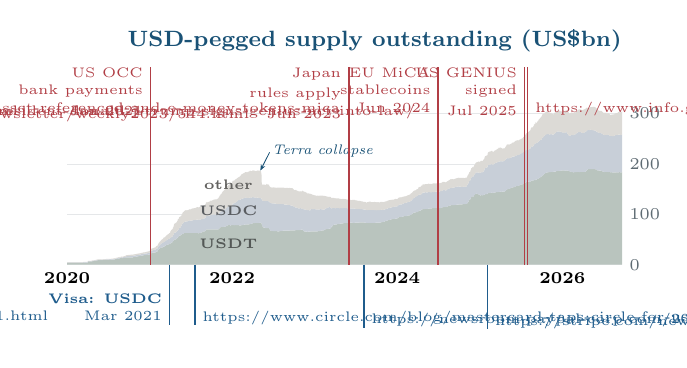
\begin{tikzpicture}[x=1cm,y=1cm,every node/.style={inner sep=0pt,font=\fontsize{6.3}{7.4}\selectfont,text=Ink}]
\definecolor{RegulationRed}{HTML}{B13E45}
\definecolor{ProviderBlue}{HTML}{1F5C8C}
\definecolor{SupplyYellow}{HTML}{F1D986}
\path[use as bounding box] (0,-2.80) rectangle (8.01,1.16);
\node[anchor=east,font=\fontsize{8.0}{9.4}\selectfont\bfseries,text=Rust] at (7.550,.99) {USD-pegged supply outstanding (US\$bn)};
% Keep the narrower plot anchored at its existing right edge.
\begin{scope}[overlay,xshift=-.00025cm,xscale=1.00,yshift=-.30cm]
\draw[Quiet!16!Paper,line width=.25pt] (0.500,-1.550)--(7.550,-1.550);
\node[anchor=west,text=Quiet,font=\fontsize{6}{7}\selectfont] at (7.6375,-1.550) {0};
\draw[Quiet!16!Paper,line width=.25pt] (0.500,-0.910)--(7.550,-0.910);
\node[anchor=west,text=Quiet,font=\fontsize{6}{7}\selectfont] at (7.6375,-0.910) {100};
\draw[Quiet!16!Paper,line width=.25pt] (0.500,-0.270)--(7.550,-0.270);
\node[anchor=west,text=Quiet,font=\fontsize{6}{7}\selectfont] at (7.6375,-0.270) {200};
\draw[Quiet!16!Paper,line width=.25pt] (0.500,0.370)--(7.550,0.370);
\node[anchor=west,text=Quiet,font=\fontsize{6}{7}\selectfont] at (7.6375,0.370) {300};
\node[anchor=north,text=black,font=\fontsize{6}{7}\selectfont\bfseries] at (0.500,-1.650) {2020};
\node[anchor=north,text=black,font=\fontsize{6}{7}\selectfont\bfseries] at (2.597,-1.650) {2022};
\node[anchor=north,text=black,font=\fontsize{6}{7}\selectfont\bfseries] at (4.692,-1.650) {2024};
\node[anchor=north,text=black,font=\fontsize{6}{7}\selectfont\bfseries] at (6.790,-1.650) {2026};
\definecolor{BandUSDT}{HTML}{B9C4BE}
\definecolor{BandUSDC}{HTML}{C8CFD8}
\definecolor{BandOther}{HTML}{DCDAD6}
\path[fill=BandUSDT,draw=none] (0.5000,-1.5295) -- (0.5029,-1.5295) -- (0.5057,-1.5226) -- (0.5086,-1.5226) -- (0.5115,-1.5226) -- (0.5143,-1.5226) -- (0.5172,-1.5226) -- (0.5201,-1.5226) -- (0.5230,-1.5226) -- (0.5258,-1.5226) -- (0.5287,-1.5226) -- (0.5316,-1.5227) -- (0.5344,-1.5226) -- (0.5373,-1.5226) -- (0.5402,-1.5226) -- (0.5430,-1.5226) -- (0.5459,-1.5226) -- (0.5488,-1.5226) -- (0.5516,-1.5226) -- (0.5545,-1.5226) -- (0.5574,-1.5226) -- (0.5603,-1.5226) -- (0.5631,-1.5226) -- (0.5660,-1.5226) -- (0.5689,-1.5225) -- (0.5717,-1.5226) -- (0.5746,-1.5226) -- (0.5775,-1.5226) -- (0.5803,-1.5225) -- (0.5832,-1.5226) -- (0.5861,-1.5226) -- (0.5889,-1.5226) -- (0.5918,-1.5226) -- (0.5947,-1.5226) -- (0.5976,-1.5225) -- (0.6004,-1.5226) -- (0.6033,-1.5226) -- (0.6062,-1.5226) -- (0.6090,-1.5226) -- (0.6119,-1.5226) -- (0.6148,-1.5225) -- (0.6176,-1.5225) -- (0.6205,-1.5226) -- (0.6234,-1.5226) -- (0.6263,-1.5226) -- (0.6291,-1.5226) -- (0.6320,-1.5226) -- (0.6349,-1.5226) -- (0.6377,-1.5225) -- (0.6406,-1.5226) -- (0.6435,-1.5226) -- (0.6463,-1.5226) -- (0.6492,-1.5226) -- (0.6521,-1.5226) -- (0.6549,-1.5225) -- (0.6578,-1.5225) -- (0.6607,-1.5226) -- (0.6636,-1.5226) -- (0.6664,-1.5225) -- (0.6693,-1.5226) -- (0.6722,-1.5226) -- (0.6750,-1.5226) -- (0.6779,-1.5226) -- (0.6808,-1.5225) -- (0.6836,-1.5225) -- (0.6865,-1.5226) -- (0.6894,-1.5225) -- (0.6922,-1.5226) -- (0.6951,-1.5227) -- (0.6980,-1.5225) -- (0.7009,-1.5225) -- (0.7037,-1.5224) -- (0.7066,-1.5224) -- (0.7095,-1.5222) -- (0.7123,-1.5227) -- (0.7152,-1.5225) -- (0.7181,-1.5224) -- (0.7209,-1.5224) -- (0.7238,-1.5229) -- (0.7267,-1.5225) -- (0.7295,-1.5222) -- (0.7324,-1.5226) -- (0.7353,-1.5225) -- (0.7382,-1.5225) -- (0.7410,-1.5226) -- (0.7439,-1.5225) -- (0.7468,-1.5225) -- (0.7496,-1.5226) -- (0.7525,-1.5225) -- (0.7554,-1.5225) -- (0.7582,-1.5225) -- (0.7611,-1.5226) -- (0.7640,-1.5225) -- (0.7668,-1.5096) -- (0.7697,-1.5094) -- (0.7726,-1.5094) -- (0.7755,-1.5093) -- (0.7783,-1.5094) -- (0.7812,-1.5094) -- (0.7841,-1.5094) -- (0.7869,-1.5093) -- (0.7898,-1.5093) -- (0.7927,-1.5093) -- (0.7955,-1.5093) -- (0.7984,-1.5094) -- (0.8013,-1.5093) -- (0.8042,-1.5094) -- (0.8070,-1.5092) -- (0.8099,-1.5093) -- (0.8128,-1.5094) -- (0.8156,-1.5092) -- (0.8185,-1.5092) -- (0.8214,-1.5093) -- (0.8242,-1.5043) -- (0.8271,-1.5045) -- (0.8300,-1.5045) -- (0.8328,-1.5044) -- (0.8357,-1.5043) -- (0.8386,-1.5042) -- (0.8415,-1.5043) -- (0.8443,-1.5008) -- (0.8472,-1.5007) -- (0.8501,-1.5001) -- (0.8529,-1.5001) -- (0.8558,-1.4999) -- (0.8587,-1.5001) -- (0.8615,-1.4997) -- (0.8644,-1.4992) -- (0.8673,-1.4983) -- (0.8701,-1.4978) -- (0.8730,-1.4968) -- (0.8759,-1.4958) -- (0.8788,-1.4957) -- (0.8816,-1.4947) -- (0.8845,-1.4947) -- (0.8874,-1.4936) -- (0.8902,-1.4933) -- (0.8931,-1.4931) -- (0.8960,-1.4926) -- (0.8988,-1.4927) -- (0.9017,-1.4929) -- (0.9046,-1.4927) -- (0.9074,-1.4928) -- (0.9103,-1.4930) -- (0.9132,-1.4930) -- (0.9161,-1.4926) -- (0.9189,-1.4924) -- (0.9218,-1.4924) -- (0.9247,-1.4923) -- (0.9275,-1.4922) -- (0.9304,-1.4921) -- (0.9333,-1.4917) -- (0.9361,-1.4918) -- (0.9390,-1.4916) -- (0.9419,-1.4910) -- (0.9447,-1.4910) -- (0.9476,-1.4907) -- (0.9505,-1.4907) -- (0.9534,-1.4906) -- (0.9562,-1.4904) -- (0.9591,-1.4903) -- (0.9620,-1.4902) -- (0.9648,-1.4898) -- (0.9677,-1.4896) -- (0.9706,-1.4893) -- (0.9734,-1.4893) -- (0.9763,-1.4892) -- (0.9792,-1.4891) -- (0.9821,-1.4889) -- (0.9849,-1.4889) -- (0.9878,-1.4887) -- (0.9907,-1.4885) -- (0.9935,-1.4884) -- (0.9964,-1.4884) -- (0.9993,-1.4884) -- (1.0021,-1.4885) -- (1.0050,-1.4885) -- (1.0079,-1.4886) -- (1.0107,-1.4884) -- (1.0136,-1.4883) -- (1.0165,-1.4883) -- (1.0194,-1.4884) -- (1.0222,-1.4883) -- (1.0251,-1.4883) -- (1.0280,-1.4883) -- (1.0308,-1.4883) -- (1.0337,-1.4879) -- (1.0366,-1.4879) -- (1.0394,-1.4878) -- (1.0423,-1.4877) -- (1.0452,-1.4877) -- (1.0480,-1.4874) -- (1.0509,-1.4873) -- (1.0538,-1.4871) -- (1.0567,-1.4871) -- (1.0595,-1.4870) -- (1.0624,-1.4870) -- (1.0653,-1.4869) -- (1.0681,-1.4868) -- (1.0710,-1.4868) -- (1.0739,-1.4867) -- (1.0767,-1.4866) -- (1.0796,-1.4866) -- (1.0825,-1.4865) -- (1.0853,-1.4859) -- (1.0882,-1.4856) -- (1.0911,-1.4850) -- (1.0940,-1.4846) -- (1.0968,-1.4846) -- (1.0997,-1.4850) -- (1.1026,-1.4830) -- (1.1054,-1.4820) -- (1.1083,-1.4815) -- (1.1112,-1.4810) -- (1.1140,-1.4800) -- (1.1169,-1.4792) -- (1.1198,-1.4788) -- (1.1226,-1.4784) -- (1.1255,-1.4780) -- (1.1284,-1.4775) -- (1.1313,-1.4764) -- (1.1341,-1.4759) -- (1.1370,-1.4754) -- (1.1399,-1.4751) -- (1.1427,-1.4741) -- (1.1456,-1.4739) -- (1.1485,-1.4732) -- (1.1513,-1.4717) -- (1.1542,-1.4718) -- (1.1571,-1.4716) -- (1.1600,-1.4707) -- (1.1628,-1.4693) -- (1.1657,-1.4693) -- (1.1686,-1.4690) -- (1.1714,-1.4683) -- (1.1743,-1.4680) -- (1.1772,-1.4679) -- (1.1800,-1.4675) -- (1.1829,-1.4677) -- (1.1858,-1.4677) -- (1.1886,-1.4666) -- (1.1915,-1.4660) -- (1.1944,-1.4649) -- (1.1973,-1.4647) -- (1.2001,-1.4692) -- (1.2030,-1.4685) -- (1.2059,-1.4669) -- (1.2087,-1.4669) -- (1.2116,-1.4659) -- (1.2145,-1.4659) -- (1.2173,-1.4659) -- (1.2202,-1.4643) -- (1.2231,-1.4643) -- (1.2259,-1.4627) -- (1.2288,-1.4627) -- (1.2317,-1.4627) -- (1.2346,-1.4627) -- (1.2374,-1.4611) -- (1.2403,-1.4676) -- (1.2432,-1.4612) -- (1.2460,-1.4596) -- (1.2489,-1.4586) -- (1.2518,-1.4586) -- (1.2546,-1.4576) -- (1.2575,-1.4576) -- (1.2604,-1.4576) -- (1.2632,-1.4576) -- (1.2661,-1.4576) -- (1.2690,-1.4576) -- (1.2719,-1.4576) -- (1.2747,-1.4576) -- (1.2776,-1.4576) -- (1.2805,-1.4576) -- (1.2833,-1.4576) -- (1.2862,-1.4576) -- (1.2891,-1.4567) -- (1.2919,-1.4567) -- (1.2948,-1.4567) -- (1.2977,-1.4567) -- (1.3005,-1.4567) -- (1.3034,-1.4567) -- (1.3063,-1.4567) -- (1.3092,-1.4557) -- (1.3120,-1.4557) -- (1.3149,-1.4557) -- (1.3178,-1.4557) -- (1.3206,-1.4557) -- (1.3235,-1.4557) -- (1.3264,-1.4557) -- (1.3292,-1.4557) -- (1.3321,-1.4557) -- (1.3350,-1.4557) -- (1.3379,-1.4557) -- (1.3407,-1.4548) -- (1.3436,-1.4528) -- (1.3465,-1.4528) -- (1.3493,-1.4519) -- (1.3522,-1.4519) -- (1.3551,-1.4519) -- (1.3579,-1.4519) -- (1.3608,-1.4509) -- (1.3637,-1.4509) -- (1.3665,-1.4500) -- (1.3694,-1.4500) -- (1.3723,-1.4490) -- (1.3752,-1.4490) -- (1.3780,-1.4490) -- (1.3809,-1.4490) -- (1.3838,-1.4481) -- (1.3866,-1.4481) -- (1.3895,-1.4462) -- (1.3924,-1.4452) -- (1.3952,-1.4452) -- (1.3981,-1.4452) -- (1.4010,-1.4452) -- (1.4038,-1.4443) -- (1.4067,-1.4433) -- (1.4096,-1.4420) -- (1.4125,-1.4420) -- (1.4153,-1.4420) -- (1.4182,-1.4420) -- (1.4211,-1.4411) -- (1.4239,-1.4411) -- (1.4268,-1.4411) -- (1.4297,-1.4398) -- (1.4325,-1.4374) -- (1.4354,-1.4374) -- (1.4383,-1.4374) -- (1.4411,-1.4362) -- (1.4440,-1.4349) -- (1.4469,-1.4349) -- (1.4498,-1.4349) -- (1.4526,-1.4349) -- (1.4555,-1.4349) -- (1.4584,-1.4349) -- (1.4612,-1.4323) -- (1.4641,-1.4310) -- (1.4670,-1.4310) -- (1.4698,-1.4310) -- (1.4727,-1.4301) -- (1.4756,-1.4301) -- (1.4784,-1.4301) -- (1.4813,-1.4301) -- (1.4842,-1.4301) -- (1.4871,-1.4301) -- (1.4899,-1.4291) -- (1.4928,-1.4291) -- (1.4957,-1.4291) -- (1.4985,-1.4291) -- (1.5014,-1.4291) -- (1.5043,-1.4278) -- (1.5071,-1.4278) -- (1.5100,-1.4278) -- (1.5129,-1.4266) -- (1.5158,-1.4266) -- (1.5186,-1.4266) -- (1.5215,-1.4256) -- (1.5244,-1.4256) -- (1.5272,-1.4243) -- (1.5301,-1.4230) -- (1.5330,-1.4230) -- (1.5358,-1.4230) -- (1.5387,-1.4230) -- (1.5416,-1.4218) -- (1.5444,-1.4218) -- (1.5473,-1.4218) -- (1.5502,-1.4218) -- (1.5531,-1.4186) -- (1.5559,-1.4134) -- (1.5588,-1.4134) -- (1.5617,-1.4134) -- (1.5645,-1.4096) -- (1.5674,-1.4051) -- (1.5703,-1.4051) -- (1.5731,-1.4007) -- (1.5760,-1.4007) -- (1.5789,-1.4007) -- (1.5817,-1.4007) -- (1.5846,-1.3981) -- (1.5875,-1.3981) -- (1.5904,-1.3981) -- (1.5932,-1.3981) -- (1.5961,-1.3981) -- (1.5990,-1.3981) -- (1.6018,-1.3955) -- (1.6047,-1.3955) -- (1.6076,-1.3955) -- (1.6104,-1.3955) -- (1.6133,-1.3957) -- (1.6162,-1.3957) -- (1.6190,-1.3957) -- (1.6219,-1.3957) -- (1.6248,-1.3931) -- (1.6277,-1.3905) -- (1.6305,-1.3873) -- (1.6334,-1.3848) -- (1.6363,-1.3848) -- (1.6391,-1.3826) -- (1.6420,-1.3826) -- (1.6449,-1.3928) -- (1.6477,-1.3774) -- (1.6506,-1.3752) -- (1.6535,-1.3694) -- (1.6563,-1.3694) -- (1.6592,-1.3605) -- (1.6621,-1.3605) -- (1.6650,-1.3541) -- (1.6678,-1.3534) -- (1.6707,-1.3534) -- (1.6736,-1.3470) -- (1.6764,-1.3470) -- (1.6793,-1.3470) -- (1.6822,-1.3445) -- (1.6850,-1.3381) -- (1.6879,-1.3381) -- (1.6908,-1.3355) -- (1.6937,-1.3304) -- (1.6965,-1.3304) -- (1.6994,-1.3304) -- (1.7023,-1.3304) -- (1.7051,-1.3304) -- (1.7080,-1.3304) -- (1.7109,-1.3304) -- (1.7137,-1.3304) -- (1.7166,-1.3304) -- (1.7195,-1.3256) -- (1.7223,-1.3256) -- (1.7252,-1.3182) -- (1.7281,-1.3182) -- (1.7310,-1.3182) -- (1.7338,-1.3182) -- (1.7367,-1.3182) -- (1.7396,-1.3182) -- (1.7424,-1.3182) -- (1.7453,-1.3118) -- (1.7482,-1.3093) -- (1.7510,-1.3093) -- (1.7539,-1.3093) -- (1.7568,-1.3093) -- (1.7596,-1.3029) -- (1.7625,-1.2990) -- (1.7654,-1.2990) -- (1.7683,-1.2991) -- (1.7711,-1.2991) -- (1.7740,-1.2991) -- (1.7769,-1.2927) -- (1.7797,-1.2927) -- (1.7826,-1.2927) -- (1.7855,-1.2927) -- (1.7883,-1.2927) -- (1.7912,-1.2927) -- (1.7941,-1.2875) -- (1.7969,-1.2875) -- (1.7998,-1.2875) -- (1.8027,-1.2875) -- (1.8056,-1.2875) -- (1.8084,-1.2799) -- (1.8113,-1.2799) -- (1.8142,-1.2799) -- (1.8170,-1.2799) -- (1.8199,-1.2799) -- (1.8228,-1.2722) -- (1.8256,-1.2722) -- (1.8285,-1.2658) -- (1.8314,-1.2658) -- (1.8342,-1.2658) -- (1.8371,-1.2658) -- (1.8400,-1.2594) -- (1.8429,-1.2594) -- (1.8457,-1.2466) -- (1.8486,-1.2466) -- (1.8515,-1.2466) -- (1.8543,-1.2402) -- (1.8572,-1.2402) -- (1.8601,-1.2274) -- (1.8629,-1.2274) -- (1.8658,-1.2274) -- (1.8687,-1.2274) -- (1.8716,-1.2274) -- (1.8744,-1.2274) -- (1.8773,-1.2274) -- (1.8802,-1.2274) -- (1.8830,-1.2274) -- (1.8859,-1.2274) -- (1.8888,-1.2242) -- (1.8916,-1.2242) -- (1.8945,-1.2178) -- (1.8974,-1.2178) -- (1.9002,-1.2114) -- (1.9031,-1.2114) -- (1.9060,-1.1986) -- (1.9089,-1.1986) -- (1.9117,-1.1986) -- (1.9146,-1.1986) -- (1.9175,-1.1986) -- (1.9203,-1.1922) -- (1.9232,-1.1858) -- (1.9261,-1.1794) -- (1.9289,-1.1794) -- (1.9318,-1.1794) -- (1.9347,-1.1794) -- (1.9375,-1.1794) -- (1.9404,-1.1794) -- (1.9433,-1.1730) -- (1.9462,-1.1730) -- (1.9490,-1.1730) -- (1.9519,-1.1730) -- (1.9548,-1.1666) -- (1.9576,-1.1666) -- (1.9605,-1.1602) -- (1.9634,-1.1602) -- (1.9662,-1.1602) -- (1.9691,-1.1602) -- (1.9720,-1.1538) -- (1.9748,-1.1538) -- (1.9777,-1.1538) -- (1.9806,-1.1666) -- (1.9835,-1.1474) -- (1.9863,-1.1474) -- (1.9892,-1.1474) -- (1.9921,-1.1474) -- (1.9949,-1.1474) -- (1.9978,-1.1474) -- (2.0007,-1.1474) -- (2.0035,-1.1474) -- (2.0064,-1.1474) -- (2.0093,-1.1474) -- (2.0121,-1.1474) -- (2.0150,-1.1474) -- (2.0179,-1.1474) -- (2.0208,-1.1474) -- (2.0236,-1.1474) -- (2.0265,-1.1474) -- (2.0294,-1.1474) -- (2.0322,-1.1474) -- (2.0351,-1.1474) -- (2.0380,-1.1474) -- (2.0408,-1.1474) -- (2.0437,-1.1474) -- (2.0466,-1.1474) -- (2.0495,-1.1474) -- (2.0523,-1.1474) -- (2.0552,-1.1474) -- (2.0581,-1.1474) -- (2.0609,-1.1474) -- (2.0638,-1.1474) -- (2.0667,-1.1474) -- (2.0695,-1.1474) -- (2.0724,-1.1474) -- (2.0753,-1.1474) -- (2.0781,-1.1474) -- (2.0810,-1.1474) -- (2.0839,-1.1474) -- (2.0868,-1.1474) -- (2.0896,-1.1474) -- (2.0925,-1.1474) -- (2.0954,-1.1474) -- (2.0982,-1.1474) -- (2.1011,-1.1474) -- (2.1040,-1.1474) -- (2.1068,-1.1474) -- (2.1097,-1.1474) -- (2.1126,-1.1474) -- (2.1154,-1.1474) -- (2.1183,-1.1474) -- (2.1212,-1.1474) -- (2.1241,-1.1474) -- (2.1269,-1.1474) -- (2.1298,-1.1474) -- (2.1327,-1.1474) -- (2.1355,-1.1474) -- (2.1384,-1.1474) -- (2.1413,-1.1474) -- (2.1441,-1.1474) -- (2.1470,-1.1474) -- (2.1499,-1.1474) -- (2.1527,-1.1474) -- (2.1556,-1.1474) -- (2.1585,-1.1474) -- (2.1614,-1.1474) -- (2.1642,-1.1474) -- (2.1671,-1.1474) -- (2.1700,-1.1538) -- (2.1728,-1.1538) -- (2.1757,-1.1538) -- (2.1786,-1.1474) -- (2.1814,-1.1474) -- (2.1843,-1.1474) -- (2.1872,-1.1474) -- (2.1900,-1.1474) -- (2.1929,-1.1474) -- (2.1958,-1.1474) -- (2.1987,-1.1410) -- (2.2015,-1.1410) -- (2.2044,-1.1410) -- (2.2073,-1.1410) -- (2.2101,-1.1410) -- (2.2130,-1.1410) -- (2.2159,-1.1346) -- (2.2187,-1.1346) -- (2.2216,-1.1282) -- (2.2245,-1.1410) -- (2.2274,-1.1282) -- (2.2302,-1.1284) -- (2.2331,-1.1285) -- (2.2360,-1.1285) -- (2.2388,-1.1285) -- (2.2417,-1.1285) -- (2.2446,-1.1285) -- (2.2474,-1.1285) -- (2.2503,-1.1285) -- (2.2532,-1.1221) -- (2.2560,-1.1221) -- (2.2589,-1.1221) -- (2.2618,-1.1157) -- (2.2647,-1.1029) -- (2.2675,-1.1029) -- (2.2704,-1.1029) -- (2.2733,-1.1029) -- (2.2761,-1.1029) -- (2.2790,-1.1029) -- (2.2819,-1.1029) -- (2.2847,-1.1029) -- (2.2876,-1.1029) -- (2.2905,-1.1029) -- (2.2933,-1.1029) -- (2.2962,-1.1029) -- (2.2991,-1.1029) -- (2.3020,-1.1029) -- (2.3048,-1.1029) -- (2.3077,-1.1029) -- (2.3106,-1.1029) -- (2.3134,-1.1029) -- (2.3163,-1.1029) -- (2.3192,-1.1029) -- (2.3220,-1.1029) -- (2.3249,-1.1029) -- (2.3278,-1.1029) -- (2.3306,-1.1029) -- (2.3335,-1.1029) -- (2.3364,-1.1029) -- (2.3393,-1.1029) -- (2.3421,-1.1029) -- (2.3450,-1.1029) -- (2.3479,-1.1029) -- (2.3507,-1.1029) -- (2.3536,-1.1029) -- (2.3565,-1.1029) -- (2.3593,-1.1029) -- (2.3622,-1.1029) -- (2.3651,-1.1029) -- (2.3679,-1.1029) -- (2.3708,-1.1029) -- (2.3737,-1.1029) -- (2.3766,-1.1029) -- (2.3794,-1.1029) -- (2.3823,-1.1029) -- (2.3852,-1.1029) -- (2.3880,-1.1029) -- (2.3909,-1.1029) -- (2.3938,-1.1031) -- (2.3966,-1.1031) -- (2.3995,-1.1031) -- (2.4024,-1.1031) -- (2.4053,-1.1031) -- (2.4081,-1.1031) -- (2.4110,-1.1031) -- (2.4139,-1.1031) -- (2.4167,-1.1031) -- (2.4196,-1.1031) -- (2.4225,-1.1031) -- (2.4253,-1.0967) -- (2.4282,-1.0967) -- (2.4311,-1.0967) -- (2.4339,-1.0903) -- (2.4368,-1.0839) -- (2.4397,-1.0839) -- (2.4426,-1.0775) -- (2.4454,-1.0839) -- (2.4483,-1.0711) -- (2.4512,-1.0711) -- (2.4540,-1.0711) -- (2.4569,-1.0711) -- (2.4598,-1.0711) -- (2.4626,-1.0711) -- (2.4655,-1.0711) -- (2.4684,-1.0711) -- (2.4712,-1.0711) -- (2.4741,-1.0711) -- (2.4770,-1.0711) -- (2.4799,-1.0711) -- (2.4827,-1.0711) -- (2.4856,-1.0711) -- (2.4885,-1.0711) -- (2.4913,-1.0711) -- (2.4942,-1.0647) -- (2.4971,-1.0647) -- (2.4999,-1.0647) -- (2.5028,-1.0647) -- (2.5057,-1.0711) -- (2.5085,-1.0711) -- (2.5114,-1.0711) -- (2.5143,-1.0711) -- (2.5172,-1.0647) -- (2.5200,-1.0583) -- (2.5229,-1.0583) -- (2.5258,-1.0519) -- (2.5286,-1.0519) -- (2.5315,-1.0647) -- (2.5344,-1.0519) -- (2.5372,-1.0519) -- (2.5401,-1.0519) -- (2.5430,-1.0519) -- (2.5458,-1.0519) -- (2.5487,-1.0455) -- (2.5516,-1.0455) -- (2.5545,-1.0455) -- (2.5573,-1.0455) -- (2.5602,-1.0455) -- (2.5631,-1.0455) -- (2.5659,-1.0455) -- (2.5688,-1.0455) -- (2.5717,-1.0551) -- (2.5745,-1.0551) -- (2.5774,-1.0551) -- (2.5803,-1.0551) -- (2.5832,-1.0487) -- (2.5860,-1.0487) -- (2.5889,-1.0487) -- (2.5918,-1.0487) -- (2.5946,-1.0423) -- (2.5975,-1.0423) -- (2.6004,-1.0458) -- (2.6032,-1.0477) -- (2.6061,-1.0483) -- (2.6090,-1.0476) -- (2.6118,-1.0459) -- (2.6147,-1.0467) -- (2.6176,-1.0476) -- (2.6205,-1.0489) -- (2.6233,-1.0505) -- (2.6262,-1.0477) -- (2.6291,-1.0472) -- (2.6319,-1.0477) -- (2.6348,-1.0485) -- (2.6377,-1.0478) -- (2.6405,-1.0487) -- (2.6434,-1.0481) -- (2.6463,-1.0480) -- (2.6491,-1.0483) -- (2.6520,-1.0484) -- (2.6549,-1.0490) -- (2.6578,-1.0499) -- (2.6606,-1.0479) -- (2.6635,-1.0488) -- (2.6664,-1.0465) -- (2.6692,-1.0491) -- (2.6721,-1.0460) -- (2.6750,-1.0462) -- (2.6778,-1.0492) -- (2.6807,-1.0485) -- (2.6836,-1.0495) -- (2.6864,-1.0504) -- (2.6893,-1.0507) -- (2.6922,-1.0506) -- (2.6951,-1.0504) -- (2.6979,-1.0504) -- (2.7008,-1.0504) -- (2.7037,-1.0498) -- (2.7065,-1.0502) -- (2.7094,-1.0505) -- (2.7123,-1.0507) -- (2.7151,-1.0475) -- (2.7180,-1.0475) -- (2.7209,-1.0474) -- (2.7237,-1.0467) -- (2.7266,-1.0472) -- (2.7295,-1.0468) -- (2.7324,-1.0461) -- (2.7352,-1.0459) -- (2.7381,-1.0461) -- (2.7410,-1.0435) -- (2.7438,-1.0434) -- (2.7467,-1.0419) -- (2.7496,-1.0420) -- (2.7524,-1.0404) -- (2.7553,-1.0404) -- (2.7582,-1.0414) -- (2.7611,-1.0401) -- (2.7639,-1.0389) -- (2.7668,-1.0410) -- (2.7697,-1.0417) -- (2.7725,-1.0389) -- (2.7754,-1.0405) -- (2.7783,-1.0390) -- (2.7811,-1.0389) -- (2.7840,-1.0374) -- (2.7869,-1.0387) -- (2.7897,-1.0375) -- (2.7926,-1.0377) -- (2.7955,-1.0377) -- (2.7984,-1.0372) -- (2.8012,-1.0373) -- (2.8041,-1.0372) -- (2.8070,-1.0375) -- (2.8098,-1.0376) -- (2.8127,-1.0375) -- (2.8156,-1.0370) -- (2.8184,-1.0346) -- (2.8213,-1.0333) -- (2.8242,-1.0327) -- (2.8270,-1.0334) -- (2.8299,-1.0326) -- (2.8328,-1.0332) -- (2.8357,-1.0321) -- (2.8385,-1.0297) -- (2.8414,-1.0296) -- (2.8443,-1.0303) -- (2.8471,-1.0294) -- (2.8500,-1.0273) -- (2.8529,-1.0256) -- (2.8557,-1.0249) -- (2.8586,-1.0245) -- (2.8615,-1.0235) -- (2.8643,-1.0227) -- (2.8672,-1.0223) -- (2.8701,-1.0226) -- (2.8730,-1.0225) -- (2.8758,-1.0219) -- (2.8787,-1.0215) -- (2.8816,-1.0213) -- (2.8844,-1.0206) -- (2.8873,-1.0211) -- (2.8902,-1.0196) -- (2.8930,-1.0205) -- (2.8959,-1.0201) -- (2.8988,-1.0203) -- (2.9016,-1.0201) -- (2.9045,-1.0200) -- (2.9074,-1.0201) -- (2.9103,-1.0202) -- (2.9131,-1.0187) -- (2.9160,-1.0180) -- (2.9189,-1.0176) -- (2.9217,-1.0175) -- (2.9246,-1.0174) -- (2.9275,-1.0179) -- (2.9303,-1.0174) -- (2.9332,-1.0178) -- (2.9361,-1.0179) -- (2.9389,-1.0173) -- (2.9418,-1.0161) -- (2.9447,-1.0171) -- (2.9476,-1.0179) -- (2.9504,-1.0173) -- (2.9533,-1.0176) -- (2.9562,-1.0171) -- (2.9590,-1.0170) -- (2.9619,-1.0165) -- (2.9648,-1.0172) -- (2.9676,-1.0177) -- (2.9705,-1.0208) -- (2.9734,-1.0413) -- (2.9763,-1.0413) -- (2.9791,-1.0589) -- (2.9820,-1.0650) -- (2.9849,-1.0650) -- (2.9877,-1.0650) -- (2.9906,-1.0749) -- (2.9935,-1.0749) -- (2.9963,-1.0749) -- (2.9992,-1.0809) -- (3.0021,-1.0809) -- (3.0049,-1.0809) -- (3.0078,-1.0809) -- (3.0107,-1.0809) -- (3.0136,-1.0809) -- (3.0164,-1.0809) -- (3.0193,-1.0856) -- (3.0222,-1.0856) -- (3.0250,-1.0856) -- (3.0279,-1.0856) -- (3.0308,-1.0856) -- (3.0336,-1.0851) -- (3.0365,-1.0856) -- (3.0394,-1.0856) -- (3.0422,-1.0856) -- (3.0451,-1.0856) -- (3.0480,-1.0863) -- (3.0509,-1.0863) -- (3.0537,-1.0863) -- (3.0566,-1.0858) -- (3.0595,-1.0859) -- (3.0623,-1.0859) -- (3.0652,-1.0871) -- (3.0681,-1.0916) -- (3.0709,-1.0963) -- (3.0738,-1.1016) -- (3.0767,-1.1068) -- (3.0795,-1.1132) -- (3.0824,-1.1135) -- (3.0853,-1.1151) -- (3.0882,-1.1179) -- (3.0910,-1.1212) -- (3.0939,-1.1212) -- (3.0968,-1.1212) -- (3.0996,-1.1219) -- (3.1025,-1.1219) -- (3.1054,-1.1219) -- (3.1082,-1.1221) -- (3.1111,-1.1222) -- (3.1140,-1.1242) -- (3.1168,-1.1253) -- (3.1197,-1.1231) -- (3.1226,-1.1231) -- (3.1255,-1.1240) -- (3.1283,-1.1243) -- (3.1312,-1.1246) -- (3.1341,-1.1246) -- (3.1369,-1.1246) -- (3.1398,-1.1246) -- (3.1427,-1.1246) -- (3.1455,-1.1246) -- (3.1484,-1.1246) -- (3.1513,-1.1249) -- (3.1542,-1.1250) -- (3.1570,-1.1254) -- (3.1599,-1.1254) -- (3.1628,-1.1254) -- (3.1656,-1.1252) -- (3.1685,-1.1254) -- (3.1714,-1.1256) -- (3.1742,-1.1256) -- (3.1771,-1.1258) -- (3.1800,-1.1258) -- (3.1828,-1.1258) -- (3.1857,-1.1257) -- (3.1886,-1.1257) -- (3.1915,-1.1257) -- (3.1943,-1.1258) -- (3.1972,-1.1253) -- (3.2001,-1.1245) -- (3.2029,-1.1236) -- (3.2058,-1.1236) -- (3.2087,-1.1229) -- (3.2115,-1.1222) -- (3.2144,-1.1221) -- (3.2173,-1.1218) -- (3.2201,-1.1218) -- (3.2230,-1.1218) -- (3.2259,-1.1218) -- (3.2288,-1.1218) -- (3.2316,-1.1215) -- (3.2345,-1.1200) -- (3.2374,-1.1191) -- (3.2402,-1.1182) -- (3.2431,-1.1166) -- (3.2460,-1.1186) -- (3.2488,-1.1176) -- (3.2517,-1.1176) -- (3.2546,-1.1177) -- (3.2574,-1.1177) -- (3.2603,-1.1177) -- (3.2632,-1.1177) -- (3.2661,-1.1177) -- (3.2689,-1.1177) -- (3.2718,-1.1177) -- (3.2747,-1.1177) -- (3.2775,-1.1171) -- (3.2804,-1.1177) -- (3.2833,-1.1177) -- (3.2861,-1.1177) -- (3.2890,-1.1177) -- (3.2919,-1.1177) -- (3.2947,-1.1177) -- (3.2976,-1.1177) -- (3.3005,-1.1177) -- (3.3034,-1.1177) -- (3.3062,-1.1177) -- (3.3091,-1.1177) -- (3.3120,-1.1177) -- (3.3148,-1.1177) -- (3.3177,-1.1177) -- (3.3206,-1.1177) -- (3.3234,-1.1170) -- (3.3263,-1.1166) -- (3.3292,-1.1160) -- (3.3321,-1.1156) -- (3.3349,-1.1156) -- (3.3378,-1.1153) -- (3.3407,-1.1153) -- (3.3435,-1.1153) -- (3.3464,-1.1153) -- (3.3493,-1.1151) -- (3.3521,-1.1151) -- (3.3550,-1.1150) -- (3.3579,-1.1151) -- (3.3607,-1.1151) -- (3.3636,-1.1151) -- (3.3665,-1.1151) -- (3.3694,-1.1151) -- (3.3722,-1.1151) -- (3.3751,-1.1151) -- (3.3780,-1.1151) -- (3.3808,-1.1152) -- (3.3837,-1.1152) -- (3.3866,-1.1152) -- (3.3894,-1.1152) -- (3.3923,-1.1144) -- (3.3952,-1.1135) -- (3.3980,-1.1134) -- (3.4009,-1.1127) -- (3.4038,-1.1125) -- (3.4067,-1.1125) -- (3.4095,-1.1121) -- (3.4124,-1.1121) -- (3.4153,-1.1121) -- (3.4181,-1.1121) -- (3.4210,-1.1121) -- (3.4239,-1.1121) -- (3.4267,-1.1121) -- (3.4296,-1.1120) -- (3.4325,-1.1119) -- (3.4353,-1.1119) -- (3.4382,-1.1119) -- (3.4411,-1.1119) -- (3.4440,-1.1119) -- (3.4468,-1.1119) -- (3.4497,-1.1118) -- (3.4526,-1.1115) -- (3.4554,-1.1102) -- (3.4583,-1.1092) -- (3.4612,-1.1086) -- (3.4640,-1.1078) -- (3.4669,-1.1067) -- (3.4698,-1.1057) -- (3.4726,-1.1062) -- (3.4755,-1.1062) -- (3.4784,-1.1062) -- (3.4813,-1.1061) -- (3.4841,-1.1057) -- (3.4870,-1.1057) -- (3.4899,-1.1051) -- (3.4927,-1.1029) -- (3.4956,-1.1131) -- (3.4985,-1.1131) -- (3.5013,-1.1186) -- (3.5042,-1.1247) -- (3.5071,-1.1252) -- (3.5100,-1.1273) -- (3.5128,-1.1279) -- (3.5157,-1.1280) -- (3.5186,-1.1280) -- (3.5214,-1.1280) -- (3.5243,-1.1284) -- (3.5272,-1.1284) -- (3.5300,-1.1308) -- (3.5329,-1.1308) -- (3.5358,-1.1317) -- (3.5386,-1.1317) -- (3.5415,-1.1317) -- (3.5444,-1.1317) -- (3.5473,-1.1317) -- (3.5501,-1.1317) -- (3.5530,-1.1322) -- (3.5559,-1.1317) -- (3.5587,-1.1317) -- (3.5616,-1.1312) -- (3.5645,-1.1309) -- (3.5673,-1.1309) -- (3.5702,-1.1304) -- (3.5731,-1.1297) -- (3.5759,-1.1297) -- (3.5788,-1.1295) -- (3.5817,-1.1295) -- (3.5846,-1.1295) -- (3.5874,-1.1295) -- (3.5903,-1.1290) -- (3.5932,-1.1277) -- (3.5960,-1.1278) -- (3.5989,-1.1274) -- (3.6018,-1.1273) -- (3.6046,-1.1267) -- (3.6075,-1.1267) -- (3.6104,-1.1263) -- (3.6132,-1.1261) -- (3.6161,-1.1261) -- (3.6190,-1.1261) -- (3.6219,-1.1261) -- (3.6247,-1.1261) -- (3.6276,-1.1261) -- (3.6305,-1.1261) -- (3.6333,-1.1261) -- (3.6362,-1.1260) -- (3.6391,-1.1260) -- (3.6419,-1.1260) -- (3.6448,-1.1260) -- (3.6477,-1.1260) -- (3.6505,-1.1260) -- (3.6534,-1.1260) -- (3.6563,-1.1260) -- (3.6592,-1.1259) -- (3.6620,-1.1259) -- (3.6649,-1.1259) -- (3.6678,-1.1259) -- (3.6706,-1.1259) -- (3.6735,-1.1259) -- (3.6764,-1.1259) -- (3.6792,-1.1259) -- (3.6821,-1.1259) -- (3.6850,-1.1254) -- (3.6879,-1.1254) -- (3.6907,-1.1245) -- (3.6936,-1.1245) -- (3.6965,-1.1245) -- (3.6993,-1.1245) -- (3.7022,-1.1245) -- (3.7051,-1.1232) -- (3.7079,-1.1229) -- (3.7108,-1.1222) -- (3.7137,-1.1210) -- (3.7165,-1.1200) -- (3.7194,-1.1192) -- (3.7223,-1.1180) -- (3.7252,-1.1173) -- (3.7280,-1.1163) -- (3.7309,-1.1161) -- (3.7338,-1.1162) -- (3.7366,-1.1160) -- (3.7395,-1.1147) -- (3.7424,-1.1147) -- (3.7452,-1.1144) -- (3.7481,-1.1144) -- (3.7510,-1.1137) -- (3.7538,-1.1137) -- (3.7567,-1.1137) -- (3.7596,-1.1137) -- (3.7625,-1.1128) -- (3.7653,-1.1124) -- (3.7682,-1.1122) -- (3.7711,-1.1076) -- (3.7739,-1.1053) -- (3.7768,-1.1034) -- (3.7797,-1.1011) -- (3.7825,-1.1002) -- (3.7854,-1.0995) -- (3.7883,-1.0995) -- (3.7911,-1.0992) -- (3.7940,-1.0991) -- (3.7969,-1.0983) -- (3.7998,-1.0976) -- (3.8026,-1.0969) -- (3.8055,-1.0966) -- (3.8084,-1.0964) -- (3.8112,-1.0961) -- (3.8141,-1.0958) -- (3.8170,-1.0952) -- (3.8198,-1.0949) -- (3.8227,-1.0933) -- (3.8256,-1.0928) -- (3.8284,-1.0926) -- (3.8313,-1.0919) -- (3.8342,-1.0909) -- (3.8371,-1.0909) -- (3.8399,-1.0905) -- (3.8428,-1.0887) -- (3.8457,-1.0884) -- (3.8485,-1.0856) -- (3.8514,-1.0835) -- (3.8543,-1.0802) -- (3.8571,-1.0748) -- (3.8600,-1.0690) -- (3.8629,-1.0625) -- (3.8658,-1.0622) -- (3.8686,-1.0629) -- (3.8715,-1.0582) -- (3.8744,-1.0545) -- (3.8772,-1.0522) -- (3.8801,-1.0477) -- (3.8830,-1.0443) -- (3.8858,-1.0439) -- (3.8887,-1.0438) -- (3.8916,-1.0415) -- (3.8944,-1.0411) -- (3.8973,-1.0403) -- (3.9002,-1.0401) -- (3.9031,-1.0400) -- (3.9059,-1.0400) -- (3.9088,-1.0393) -- (3.9117,-1.0386) -- (3.9145,-1.0380) -- (3.9174,-1.0374) -- (3.9203,-1.0368) -- (3.9231,-1.0368) -- (3.9260,-1.0367) -- (3.9289,-1.0367) -- (3.9317,-1.0358) -- (3.9346,-1.0352) -- (3.9375,-1.0343) -- (3.9404,-1.0332) -- (3.9432,-1.0323) -- (3.9461,-1.0322) -- (3.9490,-1.0321) -- (3.9518,-1.0313) -- (3.9547,-1.0305) -- (3.9576,-1.0297) -- (3.9604,-1.0291) -- (3.9633,-1.0340) -- (3.9662,-1.0288) -- (3.9690,-1.0288) -- (3.9719,-1.0282) -- (3.9748,-1.0280) -- (3.9777,-1.0279) -- (3.9805,-1.0277) -- (3.9834,-1.0272) -- (3.9863,-1.0271) -- (3.9891,-1.0271) -- (3.9920,-1.0265) -- (3.9949,-1.0261) -- (3.9977,-1.0254) -- (4.0006,-1.0249) -- (4.0035,-1.0248) -- (4.0063,-1.0247) -- (4.0092,-1.0247) -- (4.0121,-1.0231) -- (4.0150,-1.0222) -- (4.0178,-1.0214) -- (4.0207,-1.0206) -- (4.0236,-1.0202) -- (4.0264,-1.0202) -- (4.0293,-1.0201) -- (4.0322,-1.0200) -- (4.0350,-1.0199) -- (4.0379,-1.0198) -- (4.0408,-1.0198) -- (4.0437,-1.0195) -- (4.0465,-1.0194) -- (4.0494,-1.0194) -- (4.0523,-1.0191) -- (4.0551,-1.0187) -- (4.0580,-1.0185) -- (4.0609,-1.0184) -- (4.0637,-1.0182) -- (4.0666,-1.0181) -- (4.0695,-1.0181) -- (4.0723,-1.0180) -- (4.0752,-1.0178) -- (4.0781,-1.0175) -- (4.0810,-1.0174) -- (4.0838,-1.0180) -- (4.0867,-1.0179) -- (4.0896,-1.0179) -- (4.0924,-1.0176) -- (4.0953,-1.0171) -- (4.0982,-1.0170) -- (4.1010,-1.0169) -- (4.1039,-1.0167) -- (4.1068,-1.0166) -- (4.1096,-1.0166) -- (4.1125,-1.0157) -- (4.1154,-1.0156) -- (4.1183,-1.0153) -- (4.1211,-1.0153) -- (4.1240,-1.0153) -- (4.1269,-1.0178) -- (4.1297,-1.0178) -- (4.1326,-1.0178) -- (4.1355,-1.0177) -- (4.1383,-1.0177) -- (4.1412,-1.0176) -- (4.1441,-1.0176) -- (4.1469,-1.0176) -- (4.1498,-1.0176) -- (4.1527,-1.0174) -- (4.1556,-1.0174) -- (4.1584,-1.0168) -- (4.1613,-1.0165) -- (4.1642,-1.0167) -- (4.1670,-1.0167) -- (4.1699,-1.0167) -- (4.1728,-1.0167) -- (4.1756,-1.0167) -- (4.1785,-1.0167) -- (4.1814,-1.0167) -- (4.1842,-1.0166) -- (4.1871,-1.0166) -- (4.1900,-1.0167) -- (4.1929,-1.0167) -- (4.1957,-1.0165) -- (4.1986,-1.0165) -- (4.2015,-1.0162) -- (4.2043,-1.0150) -- (4.2072,-1.0148) -- (4.2101,-1.0148) -- (4.2129,-1.0141) -- (4.2158,-1.0138) -- (4.2187,-1.0140) -- (4.2216,-1.0137) -- (4.2244,-1.0138) -- (4.2273,-1.0138) -- (4.2302,-1.0138) -- (4.2330,-1.0138) -- (4.2359,-1.0137) -- (4.2388,-1.0137) -- (4.2416,-1.0137) -- (4.2445,-1.0137) -- (4.2474,-1.0137) -- (4.2502,-1.0137) -- (4.2531,-1.0132) -- (4.2560,-1.0132) -- (4.2589,-1.0132) -- (4.2617,-1.0132) -- (4.2646,-1.0132) -- (4.2675,-1.0132) -- (4.2703,-1.0132) -- (4.2732,-1.0152) -- (4.2761,-1.0155) -- (4.2789,-1.0155) -- (4.2818,-1.0155) -- (4.2847,-1.0163) -- (4.2875,-1.0163) -- (4.2904,-1.0163) -- (4.2933,-1.0163) -- (4.2962,-1.0178) -- (4.2990,-1.0188) -- (4.3019,-1.0200) -- (4.3048,-1.0199) -- (4.3076,-1.0199) -- (4.3105,-1.0199) -- (4.3134,-1.0199) -- (4.3162,-1.0199) -- (4.3191,-1.0199) -- (4.3220,-1.0199) -- (4.3248,-1.0199) -- (4.3277,-1.0199) -- (4.3306,-1.0199) -- (4.3335,-1.0199) -- (4.3363,-1.0198) -- (4.3392,-1.0198) -- (4.3421,-1.0198) -- (4.3449,-1.0196) -- (4.3478,-1.0196) -- (4.3507,-1.0196) -- (4.3535,-1.0196) -- (4.3564,-1.0195) -- (4.3593,-1.0195) -- (4.3621,-1.0195) -- (4.3650,-1.0188) -- (4.3679,-1.0188) -- (4.3708,-1.0188) -- (4.3736,-1.0188) -- (4.3765,-1.0187) -- (4.3794,-1.0187) -- (4.3822,-1.0187) -- (4.3851,-1.0187) -- (4.3880,-1.0187) -- (4.3908,-1.0187) -- (4.3937,-1.0184) -- (4.3966,-1.0179) -- (4.3995,-1.0177) -- (4.4023,-1.0177) -- (4.4052,-1.0177) -- (4.4081,-1.0176) -- (4.4109,-1.0176) -- (4.4138,-1.0176) -- (4.4167,-1.0172) -- (4.4195,-1.0172) -- (4.4224,-1.0172) -- (4.4253,-1.0174) -- (4.4281,-1.0173) -- (4.4310,-1.0173) -- (4.4339,-1.0168) -- (4.4368,-1.0166) -- (4.4396,-1.0166) -- (4.4425,-1.0164) -- (4.4454,-1.0162) -- (4.4482,-1.0159) -- (4.4511,-1.0159) -- (4.4540,-1.0158) -- (4.4568,-1.0157) -- (4.4597,-1.0156) -- (4.4626,-1.0156) -- (4.4654,-1.0156) -- (4.4683,-1.0156) -- (4.4712,-1.0155) -- (4.4741,-1.0152) -- (4.4769,-1.0146) -- (4.4798,-1.0137) -- (4.4827,-1.0130) -- (4.4855,-1.0116) -- (4.4884,-1.0116) -- (4.4913,-1.0115) -- (4.4941,-1.0107) -- (4.4970,-1.0109) -- (4.4999,-1.0100) -- (4.5027,-1.0093) -- (4.5056,-1.0091) -- (4.5085,-1.0091) -- (4.5114,-1.0091) -- (4.5142,-1.0088) -- (4.5171,-1.0074) -- (4.5200,-1.0070) -- (4.5228,-1.0049) -- (4.5257,-1.0039) -- (4.5286,-1.0038) -- (4.5314,-1.0036) -- (4.5343,-1.0014) -- (4.5372,-0.9992) -- (4.5400,-0.9981) -- (4.5429,-0.9965) -- (4.5458,-0.9954) -- (4.5487,-0.9947) -- (4.5515,-0.9946) -- (4.5544,-0.9929) -- (4.5573,-0.9913) -- (4.5601,-0.9906) -- (4.5630,-0.9900) -- (4.5659,-0.9890) -- (4.5687,-0.9889) -- (4.5716,-0.9888) -- (4.5745,-0.9868) -- (4.5774,-0.9850) -- (4.5802,-0.9839) -- (4.5831,-0.9837) -- (4.5860,-0.9824) -- (4.5888,-0.9823) -- (4.5917,-0.9820) -- (4.5946,-0.9811) -- (4.5974,-0.9801) -- (4.6003,-0.9788) -- (4.6032,-0.9784) -- (4.6060,-0.9772) -- (4.6089,-0.9768) -- (4.6118,-0.9764) -- (4.6147,-0.9754) -- (4.6175,-0.9740) -- (4.6204,-0.9737) -- (4.6233,-0.9725) -- (4.6261,-0.9720) -- (4.6290,-0.9704) -- (4.6319,-0.9707) -- (4.6347,-0.9701) -- (4.6376,-0.9700) -- (4.6405,-0.9700) -- (4.6433,-0.9689) -- (4.6462,-0.9683) -- (4.6491,-0.9683) -- (4.6520,-0.9683) -- (4.6548,-0.9683) -- (4.6577,-0.9682) -- (4.6606,-0.9676) -- (4.6634,-0.9673) -- (4.6663,-0.9665) -- (4.6692,-0.9661) -- (4.6720,-0.9658) -- (4.6749,-0.9657) -- (4.6778,-0.9656) -- (4.6806,-0.9649) -- (4.6835,-0.9644) -- (4.6864,-0.9634) -- (4.6893,-0.9633) -- (4.6921,-0.9633) -- (4.6950,-0.9632) -- (4.6979,-0.9611) -- (4.7007,-0.9586) -- (4.7036,-0.9562) -- (4.7065,-0.9527) -- (4.7093,-0.9514) -- (4.7122,-0.9510) -- (4.7151,-0.9480) -- (4.7179,-0.9460) -- (4.7208,-0.9446) -- (4.7237,-0.9421) -- (4.7266,-0.9421) -- (4.7294,-0.9421) -- (4.7323,-0.9421) -- (4.7352,-0.9414) -- (4.7380,-0.9414) -- (4.7409,-0.9411) -- (4.7438,-0.9418) -- (4.7466,-0.9418) -- (4.7495,-0.9418) -- (4.7524,-0.9426) -- (4.7553,-0.9429) -- (4.7581,-0.9384) -- (4.7610,-0.9385) -- (4.7639,-0.9385) -- (4.7667,-0.9354) -- (4.7696,-0.9355) -- (4.7725,-0.9355) -- (4.7753,-0.9353) -- (4.7782,-0.9344) -- (4.7811,-0.9343) -- (4.7839,-0.9343) -- (4.7868,-0.9342) -- (4.7897,-0.9342) -- (4.7926,-0.9342) -- (4.7954,-0.9342) -- (4.7983,-0.9345) -- (4.8012,-0.9345) -- (4.8040,-0.9344) -- (4.8069,-0.9343) -- (4.8098,-0.9335) -- (4.8126,-0.9326) -- (4.8155,-0.9314) -- (4.8184,-0.9306) -- (4.8212,-0.9295) -- (4.8241,-0.9271) -- (4.8270,-0.9258) -- (4.8299,-0.9251) -- (4.8327,-0.9249) -- (4.8356,-0.9248) -- (4.8385,-0.9240) -- (4.8413,-0.9239) -- (4.8442,-0.9239) -- (4.8471,-0.9235) -- (4.8499,-0.9235) -- (4.8528,-0.9235) -- (4.8557,-0.9221) -- (4.8585,-0.9204) -- (4.8614,-0.9183) -- (4.8643,-0.9175) -- (4.8672,-0.9153) -- (4.8700,-0.9137) -- (4.8729,-0.9130) -- (4.8758,-0.9098) -- (4.8786,-0.9072) -- (4.8815,-0.9052) -- (4.8844,-0.9033) -- (4.8872,-0.8998) -- (4.8901,-0.8984) -- (4.8930,-0.8971) -- (4.8958,-0.8945) -- (4.8987,-0.8930) -- (4.9016,-0.8900) -- (4.9045,-0.8892) -- (4.9073,-0.8888) -- (4.9102,-0.8882) -- (4.9131,-0.8882) -- (4.9159,-0.8866) -- (4.9188,-0.8859) -- (4.9217,-0.8851) -- (4.9245,-0.8841) -- (4.9274,-0.8844) -- (4.9303,-0.8844) -- (4.9332,-0.8844) -- (4.9360,-0.8829) -- (4.9389,-0.8821) -- (4.9418,-0.8816) -- (4.9446,-0.8813) -- (4.9475,-0.8813) -- (4.9504,-0.8813) -- (4.9532,-0.8816) -- (4.9561,-0.8803) -- (4.9590,-0.8763) -- (4.9618,-0.8708) -- (4.9647,-0.8679) -- (4.9676,-0.8665) -- (4.9705,-0.8660) -- (4.9733,-0.8660) -- (4.9762,-0.8650) -- (4.9791,-0.8642) -- (4.9819,-0.8637) -- (4.9848,-0.8634) -- (4.9877,-0.8631) -- (4.9905,-0.8610) -- (4.9934,-0.8608) -- (4.9963,-0.8584) -- (4.9991,-0.8541) -- (5.0020,-0.8518) -- (5.0049,-0.8491) -- (5.0078,-0.8472) -- (5.0106,-0.8471) -- (5.0135,-0.8471) -- (5.0164,-0.8449) -- (5.0192,-0.8436) -- (5.0221,-0.8436) -- (5.0250,-0.8436) -- (5.0278,-0.8436) -- (5.0307,-0.8438) -- (5.0336,-0.8438) -- (5.0364,-0.8434) -- (5.0393,-0.8434) -- (5.0422,-0.8438) -- (5.0451,-0.8438) -- (5.0479,-0.8428) -- (5.0508,-0.8419) -- (5.0537,-0.8419) -- (5.0565,-0.8407) -- (5.0594,-0.8410) -- (5.0623,-0.8409) -- (5.0651,-0.8413) -- (5.0680,-0.8421) -- (5.0709,-0.8421) -- (5.0737,-0.8422) -- (5.0766,-0.8422) -- (5.0795,-0.8416) -- (5.0824,-0.8414) -- (5.0852,-0.8402) -- (5.0881,-0.8394) -- (5.0910,-0.8388) -- (5.0938,-0.8388) -- (5.0967,-0.8392) -- (5.0996,-0.8369) -- (5.1024,-0.8367) -- (5.1053,-0.8358) -- (5.1082,-0.8358) -- (5.1111,-0.8358) -- (5.1139,-0.8358) -- (5.1168,-0.8357) -- (5.1197,-0.8357) -- (5.1225,-0.8357) -- (5.1254,-0.8357) -- (5.1283,-0.8347) -- (5.1311,-0.8343) -- (5.1340,-0.8345) -- (5.1369,-0.8316) -- (5.1397,-0.8316) -- (5.1426,-0.8312) -- (5.1455,-0.8309) -- (5.1484,-0.8308) -- (5.1512,-0.8308) -- (5.1541,-0.8306) -- (5.1570,-0.8306) -- (5.1598,-0.8306) -- (5.1627,-0.8303) -- (5.1656,-0.8303) -- (5.1684,-0.8302) -- (5.1713,-0.8302) -- (5.1742,-0.8302) -- (5.1770,-0.8302) -- (5.1799,-0.8299) -- (5.1828,-0.8299) -- (5.1857,-0.8281) -- (5.1885,-0.8280) -- (5.1914,-0.8278) -- (5.1943,-0.8278) -- (5.1971,-0.8278) -- (5.2000,-0.8285) -- (5.2029,-0.8291) -- (5.2057,-0.8290) -- (5.2086,-0.8288) -- (5.2115,-0.8282) -- (5.2143,-0.8285) -- (5.2172,-0.8290) -- (5.2201,-0.8300) -- (5.2230,-0.8302) -- (5.2258,-0.8309) -- (5.2287,-0.8316) -- (5.2316,-0.8317) -- (5.2344,-0.8317) -- (5.2373,-0.8317) -- (5.2402,-0.8315) -- (5.2430,-0.8309) -- (5.2459,-0.8308) -- (5.2488,-0.8320) -- (5.2516,-0.8302) -- (5.2545,-0.8298) -- (5.2574,-0.8277) -- (5.2603,-0.8254) -- (5.2631,-0.8228) -- (5.2660,-0.8225) -- (5.2689,-0.8213) -- (5.2717,-0.8203) -- (5.2746,-0.8200) -- (5.2775,-0.8184) -- (5.2803,-0.8174) -- (5.2832,-0.8175) -- (5.2861,-0.8182) -- (5.2889,-0.8180) -- (5.2918,-0.8174) -- (5.2947,-0.8174) -- (5.2976,-0.8171) -- (5.3004,-0.8171) -- (5.3033,-0.8169) -- (5.3062,-0.8169) -- (5.3090,-0.8166) -- (5.3119,-0.8167) -- (5.3148,-0.8167) -- (5.3176,-0.8175) -- (5.3205,-0.8167) -- (5.3234,-0.8142) -- (5.3263,-0.8113) -- (5.3291,-0.8103) -- (5.3320,-0.8099) -- (5.3349,-0.8099) -- (5.3377,-0.8083) -- (5.3406,-0.8068) -- (5.3435,-0.8042) -- (5.3463,-0.8031) -- (5.3492,-0.8023) -- (5.3521,-0.8019) -- (5.3549,-0.8019) -- (5.3578,-0.8012) -- (5.3607,-0.7994) -- (5.3636,-0.7986) -- (5.3664,-0.7971) -- (5.3693,-0.7966) -- (5.3722,-0.7958) -- (5.3750,-0.7958) -- (5.3779,-0.7949) -- (5.3808,-0.7952) -- (5.3836,-0.7942) -- (5.3865,-0.7935) -- (5.3894,-0.7935) -- (5.3922,-0.7935) -- (5.3951,-0.7934) -- (5.3980,-0.7940) -- (5.4009,-0.7940) -- (5.4037,-0.7939) -- (5.4066,-0.7940) -- (5.4095,-0.7937) -- (5.4123,-0.7937) -- (5.4152,-0.7937) -- (5.4181,-0.7921) -- (5.4209,-0.7920) -- (5.4238,-0.7920) -- (5.4267,-0.7923) -- (5.4295,-0.7909) -- (5.4324,-0.7881) -- (5.4353,-0.7896) -- (5.4382,-0.7901) -- (5.4410,-0.7893) -- (5.4439,-0.7891) -- (5.4468,-0.7880) -- (5.4496,-0.7874) -- (5.4525,-0.7874) -- (5.4554,-0.7874) -- (5.4582,-0.7869) -- (5.4611,-0.7869) -- (5.4640,-0.7866) -- (5.4668,-0.7862) -- (5.4697,-0.7858) -- (5.4726,-0.7858) -- (5.4755,-0.7844) -- (5.4783,-0.7842) -- (5.4812,-0.7842) -- (5.4841,-0.7843) -- (5.4869,-0.7843) -- (5.4898,-0.7842) -- (5.4927,-0.7841) -- (5.4955,-0.7841) -- (5.4984,-0.7830) -- (5.5013,-0.7830) -- (5.5042,-0.7830) -- (5.5070,-0.7838) -- (5.5099,-0.7837) -- (5.5128,-0.7837) -- (5.5156,-0.7837) -- (5.5185,-0.7835) -- (5.5214,-0.7833) -- (5.5242,-0.7822) -- (5.5271,-0.7820) -- (5.5300,-0.7814) -- (5.5328,-0.7810) -- (5.5357,-0.7809) -- (5.5386,-0.7807) -- (5.5415,-0.7808) -- (5.5443,-0.7807) -- (5.5472,-0.7804) -- (5.5501,-0.7802) -- (5.5529,-0.7800) -- (5.5558,-0.7800) -- (5.5587,-0.7808) -- (5.5615,-0.7790) -- (5.5644,-0.7786) -- (5.5673,-0.7789) -- (5.5701,-0.7786) -- (5.5730,-0.7783) -- (5.5759,-0.7783) -- (5.5788,-0.7723) -- (5.5816,-0.7723) -- (5.5845,-0.7692) -- (5.5874,-0.7661) -- (5.5902,-0.7601) -- (5.5931,-0.7584) -- (5.5960,-0.7566) -- (5.5988,-0.7449) -- (5.6017,-0.7397) -- (5.6046,-0.7334) -- (5.6074,-0.7232) -- (5.6103,-0.7232) -- (5.6132,-0.7217) -- (5.6161,-0.7208) -- (5.6189,-0.7215) -- (5.6218,-0.7184) -- (5.6247,-0.7100) -- (5.6275,-0.7080) -- (5.6304,-0.6996) -- (5.6333,-0.6923) -- (5.6361,-0.6897) -- (5.6390,-0.6880) -- (5.6419,-0.6878) -- (5.6447,-0.6851) -- (5.6476,-0.6798) -- (5.6505,-0.6779) -- (5.6534,-0.6899) -- (5.6562,-0.6894) -- (5.6591,-0.6859) -- (5.6620,-0.6838) -- (5.6648,-0.6793) -- (5.6677,-0.6734) -- (5.6706,-0.6666) -- (5.6734,-0.6651) -- (5.6763,-0.6642) -- (5.6792,-0.6627) -- (5.6821,-0.6607) -- (5.6849,-0.6540) -- (5.6878,-0.6514) -- (5.6907,-0.6511) -- (5.6935,-0.6504) -- (5.6964,-0.6504) -- (5.6993,-0.6491) -- (5.7021,-0.6482) -- (5.7050,-0.6480) -- (5.7079,-0.6483) -- (5.7107,-0.6510) -- (5.7136,-0.6529) -- (5.7165,-0.6530) -- (5.7194,-0.6553) -- (5.7222,-0.6557) -- (5.7251,-0.6557) -- (5.7280,-0.6556) -- (5.7308,-0.6566) -- (5.7337,-0.6584) -- (5.7366,-0.6588) -- (5.7394,-0.6661) -- (5.7423,-0.6684) -- (5.7452,-0.6696) -- (5.7480,-0.6696) -- (5.7509,-0.6696) -- (5.7538,-0.6696) -- (5.7567,-0.6696) -- (5.7595,-0.6675) -- (5.7624,-0.6686) -- (5.7653,-0.6672) -- (5.7681,-0.6682) -- (5.7710,-0.6682) -- (5.7739,-0.6684) -- (5.7767,-0.6681) -- (5.7796,-0.6695) -- (5.7825,-0.6695) -- (5.7853,-0.6681) -- (5.7882,-0.6681) -- (5.7911,-0.6629) -- (5.7940,-0.6624) -- (5.7968,-0.6623) -- (5.7997,-0.6619) -- (5.8026,-0.6614) -- (5.8054,-0.6594) -- (5.8083,-0.6589) -- (5.8112,-0.6554) -- (5.8140,-0.6554) -- (5.8169,-0.6553) -- (5.8198,-0.6545) -- (5.8226,-0.6545) -- (5.8255,-0.6541) -- (5.8284,-0.6540) -- (5.8313,-0.6541) -- (5.8341,-0.6541) -- (5.8370,-0.6542) -- (5.8399,-0.6544) -- (5.8427,-0.6458) -- (5.8456,-0.6420) -- (5.8485,-0.6423) -- (5.8513,-0.6404) -- (5.8542,-0.6399) -- (5.8571,-0.6400) -- (5.8600,-0.6390) -- (5.8628,-0.6395) -- (5.8657,-0.6385) -- (5.8686,-0.6398) -- (5.8714,-0.6386) -- (5.8743,-0.6386) -- (5.8772,-0.6386) -- (5.8800,-0.6396) -- (5.8829,-0.6407) -- (5.8858,-0.6368) -- (5.8886,-0.6358) -- (5.8915,-0.6351) -- (5.8944,-0.6351) -- (5.8973,-0.6356) -- (5.9001,-0.6360) -- (5.9030,-0.6378) -- (5.9059,-0.6385) -- (5.9087,-0.6373) -- (5.9116,-0.6371) -- (5.9145,-0.6364) -- (5.9173,-0.6360) -- (5.9202,-0.6356) -- (5.9231,-0.6356) -- (5.9259,-0.6342) -- (5.9288,-0.6337) -- (5.9317,-0.6333) -- (5.9346,-0.6330) -- (5.9374,-0.6330) -- (5.9403,-0.6326) -- (5.9432,-0.6312) -- (5.9460,-0.6300) -- (5.9489,-0.6300) -- (5.9518,-0.6294) -- (5.9546,-0.6294) -- (5.9575,-0.6294) -- (5.9604,-0.6278) -- (5.9632,-0.6278) -- (5.9661,-0.6266) -- (5.9690,-0.6288) -- (5.9719,-0.6272) -- (5.9747,-0.6270) -- (5.9776,-0.6270) -- (5.9805,-0.6255) -- (5.9833,-0.6239) -- (5.9862,-0.6228) -- (5.9891,-0.6227) -- (5.9919,-0.6251) -- (5.9948,-0.6251) -- (5.9977,-0.6242) -- (6.0005,-0.6237) -- (6.0034,-0.6236) -- (6.0063,-0.6232) -- (6.0092,-0.6234) -- (6.0120,-0.6234) -- (6.0149,-0.6235) -- (6.0178,-0.6248) -- (6.0206,-0.6227) -- (6.0235,-0.6239) -- (6.0264,-0.6217) -- (6.0292,-0.6230) -- (6.0321,-0.6223) -- (6.0350,-0.6207) -- (6.0379,-0.6220) -- (6.0407,-0.6221) -- (6.0436,-0.6205) -- (6.0465,-0.6194) -- (6.0493,-0.6194) -- (6.0522,-0.6218) -- (6.0551,-0.6206) -- (6.0579,-0.6207) -- (6.0608,-0.6204) -- (6.0637,-0.6171) -- (6.0665,-0.6147) -- (6.0694,-0.6119) -- (6.0723,-0.6103) -- (6.0752,-0.6048) -- (6.0780,-0.6035) -- (6.0809,-0.5989) -- (6.0838,-0.5970) -- (6.0866,-0.5943) -- (6.0895,-0.5936) -- (6.0924,-0.5918) -- (6.0952,-0.5901) -- (6.0981,-0.5901) -- (6.1010,-0.5911) -- (6.1038,-0.5893) -- (6.1067,-0.5888) -- (6.1096,-0.5878) -- (6.1125,-0.5875) -- (6.1153,-0.5867) -- (6.1182,-0.5861) -- (6.1211,-0.5858) -- (6.1239,-0.5841) -- (6.1268,-0.5815) -- (6.1297,-0.5788) -- (6.1325,-0.5785) -- (6.1354,-0.5778) -- (6.1383,-0.5769) -- (6.1411,-0.5754) -- (6.1440,-0.5742) -- (6.1469,-0.5720) -- (6.1498,-0.5700) -- (6.1526,-0.5687) -- (6.1555,-0.5685) -- (6.1584,-0.5685) -- (6.1612,-0.5686) -- (6.1641,-0.5673) -- (6.1670,-0.5670) -- (6.1698,-0.5664) -- (6.1727,-0.5666) -- (6.1756,-0.5662) -- (6.1784,-0.5659) -- (6.1813,-0.5649) -- (6.1842,-0.5626) -- (6.1871,-0.5613) -- (6.1899,-0.5605) -- (6.1928,-0.5573) -- (6.1957,-0.5554) -- (6.1985,-0.5554) -- (6.2014,-0.5515) -- (6.2043,-0.5537) -- (6.2071,-0.5514) -- (6.2100,-0.5514) -- (6.2129,-0.5496) -- (6.2158,-0.5498) -- (6.2186,-0.5499) -- (6.2215,-0.5494) -- (6.2244,-0.5491) -- (6.2272,-0.5484) -- (6.2301,-0.5473) -- (6.2330,-0.5472) -- (6.2358,-0.5478) -- (6.2387,-0.5468) -- (6.2416,-0.5522) -- (6.2444,-0.5427) -- (6.2473,-0.5393) -- (6.2502,-0.5371) -- (6.2531,-0.5369) -- (6.2559,-0.5360) -- (6.2588,-0.5355) -- (6.2617,-0.5340) -- (6.2645,-0.5344) -- (6.2674,-0.5314) -- (6.2703,-0.5304) -- (6.2731,-0.5293) -- (6.2760,-0.5293) -- (6.2789,-0.5294) -- (6.2817,-0.5291) -- (6.2846,-0.5295) -- (6.2875,-0.5279) -- (6.2904,-0.5260) -- (6.2932,-0.5250) -- (6.2961,-0.5235) -- (6.2990,-0.5235) -- (6.3018,-0.5225) -- (6.3047,-0.5217) -- (6.3076,-0.5129) -- (6.3104,-0.5166) -- (6.3133,-0.5133) -- (6.3162,-0.5109) -- (6.3190,-0.5098) -- (6.3219,-0.5077) -- (6.3248,-0.5066) -- (6.3277,-0.5055) -- (6.3305,-0.5010) -- (6.3334,-0.5010) -- (6.3363,-0.4976) -- (6.3391,-0.4976) -- (6.3420,-0.4987) -- (6.3449,-0.4980) -- (6.3477,-0.4967) -- (6.3506,-0.4960) -- (6.3535,-0.4955) -- (6.3563,-0.4955) -- (6.3592,-0.4957) -- (6.3621,-0.4958) -- (6.3650,-0.4956) -- (6.3678,-0.4971) -- (6.3707,-0.4928) -- (6.3736,-0.4937) -- (6.3764,-0.4923) -- (6.3793,-0.4968) -- (6.3822,-0.4948) -- (6.3850,-0.4967) -- (6.3879,-0.4934) -- (6.3908,-0.4866) -- (6.3937,-0.4855) -- (6.3965,-0.4855) -- (6.3994,-0.4812) -- (6.4023,-0.4801) -- (6.4051,-0.4795) -- (6.4080,-0.4795) -- (6.4109,-0.4817) -- (6.4137,-0.4817) -- (6.4166,-0.4806) -- (6.4195,-0.4798) -- (6.4223,-0.4797) -- (6.4252,-0.4798) -- (6.4281,-0.4787) -- (6.4310,-0.4721) -- (6.4338,-0.4774) -- (6.4367,-0.4748) -- (6.4396,-0.4751) -- (6.4424,-0.4749) -- (6.4453,-0.4820) -- (6.4482,-0.4730) -- (6.4510,-0.4582) -- (6.4539,-0.4695) -- (6.4568,-0.4695) -- (6.4596,-0.4695) -- (6.4625,-0.4692) -- (6.4654,-0.4681) -- (6.4683,-0.4658) -- (6.4711,-0.4651) -- (6.4740,-0.4613) -- (6.4769,-0.4597) -- (6.4797,-0.4609) -- (6.4826,-0.4580) -- (6.4855,-0.4562) -- (6.4883,-0.4542) -- (6.4912,-0.4531) -- (6.4941,-0.4491) -- (6.4969,-0.4474) -- (6.4998,-0.4494) -- (6.5027,-0.4448) -- (6.5056,-0.4427) -- (6.5084,-0.4406) -- (6.5113,-0.4402) -- (6.5142,-0.4353) -- (6.5170,-0.4340) -- (6.5199,-0.4343) -- (6.5228,-0.4326) -- (6.5256,-0.4308) -- (6.5285,-0.4270) -- (6.5314,-0.4226) -- (6.5342,-0.4197) -- (6.5371,-0.4172) -- (6.5400,-0.4180) -- (6.5429,-0.4147) -- (6.5457,-0.4116) -- (6.5486,-0.4105) -- (6.5515,-0.4145) -- (6.5543,-0.4041) -- (6.5572,-0.3989) -- (6.5601,-0.3981) -- (6.5629,-0.3972) -- (6.5658,-0.3943) -- (6.5687,-0.3897) -- (6.5716,-0.3890) -- (6.5744,-0.3876) -- (6.5773,-0.3863) -- (6.5802,-0.3863) -- (6.5830,-0.3850) -- (6.5859,-0.3818) -- (6.5888,-0.3822) -- (6.5916,-0.3806) -- (6.5945,-0.3786) -- (6.5974,-0.3786) -- (6.6002,-0.3779) -- (6.6031,-0.3776) -- (6.6060,-0.3761) -- (6.6089,-0.3765) -- (6.6117,-0.3765) -- (6.6146,-0.3761) -- (6.6175,-0.3757) -- (6.6203,-0.3752) -- (6.6232,-0.3752) -- (6.6261,-0.3767) -- (6.6289,-0.3754) -- (6.6318,-0.3761) -- (6.6347,-0.3747) -- (6.6375,-0.3760) -- (6.6404,-0.3760) -- (6.6433,-0.3758) -- (6.6462,-0.3752) -- (6.6490,-0.3713) -- (6.6519,-0.3722) -- (6.6548,-0.3724) -- (6.6576,-0.3723) -- (6.6605,-0.3723) -- (6.6634,-0.3724) -- (6.6662,-0.3733) -- (6.6691,-0.3732) -- (6.6720,-0.3675) -- (6.6748,-0.3688) -- (6.6777,-0.3688) -- (6.6806,-0.3700) -- (6.6835,-0.3691) -- (6.6863,-0.3692) -- (6.6892,-0.3689) -- (6.6921,-0.3689) -- (6.6949,-0.3686) -- (6.6978,-0.3687) -- (6.7007,-0.3687) -- (6.7035,-0.3688) -- (6.7064,-0.3682) -- (6.7093,-0.3642) -- (6.7121,-0.3629) -- (6.7150,-0.3617) -- (6.7179,-0.3621) -- (6.7208,-0.3620) -- (6.7236,-0.3616) -- (6.7265,-0.3585) -- (6.7294,-0.3591) -- (6.7322,-0.3588) -- (6.7351,-0.3581) -- (6.7380,-0.3582) -- (6.7408,-0.3582) -- (6.7437,-0.3576) -- (6.7466,-0.3577) -- (6.7495,-0.3577) -- (6.7523,-0.3580) -- (6.7552,-0.3572) -- (6.7581,-0.3545) -- (6.7609,-0.3545) -- (6.7638,-0.3540) -- (6.7667,-0.3526) -- (6.7695,-0.3541) -- (6.7724,-0.3541) -- (6.7753,-0.3541) -- (6.7781,-0.3545) -- (6.7810,-0.3545) -- (6.7839,-0.3513) -- (6.7868,-0.3512) -- (6.7896,-0.3515) -- (6.7925,-0.3527) -- (6.7954,-0.3518) -- (6.7982,-0.3527) -- (6.8011,-0.3527) -- (6.8040,-0.3513) -- (6.8068,-0.3528) -- (6.8097,-0.3528) -- (6.8126,-0.3585) -- (6.8154,-0.3536) -- (6.8183,-0.3529) -- (6.8212,-0.3536) -- (6.8241,-0.3538) -- (6.8269,-0.3543) -- (6.8298,-0.3545) -- (6.8327,-0.3553) -- (6.8355,-0.3554) -- (6.8384,-0.3554) -- (6.8413,-0.3534) -- (6.8441,-0.3534) -- (6.8470,-0.3533) -- (6.8499,-0.3539) -- (6.8527,-0.3539) -- (6.8556,-0.3540) -- (6.8585,-0.3540) -- (6.8614,-0.3541) -- (6.8642,-0.3563) -- (6.8671,-0.3571) -- (6.8700,-0.3577) -- (6.8728,-0.3608) -- (6.8757,-0.3623) -- (6.8786,-0.3638) -- (6.8814,-0.3634) -- (6.8843,-0.3641) -- (6.8872,-0.3650) -- (6.8900,-0.3616) -- (6.8929,-0.3643) -- (6.8958,-0.3751) -- (6.8987,-0.3759) -- (6.9015,-0.3689) -- (6.9044,-0.3693) -- (6.9073,-0.3701) -- (6.9101,-0.3725) -- (6.9130,-0.3729) -- (6.9159,-0.3738) -- (6.9187,-0.3738) -- (6.9216,-0.3740) -- (6.9245,-0.3742) -- (6.9274,-0.3743) -- (6.9302,-0.3742) -- (6.9331,-0.3743) -- (6.9360,-0.3814) -- (6.9388,-0.3812) -- (6.9417,-0.3750) -- (6.9446,-0.3750) -- (6.9474,-0.3748) -- (6.9503,-0.3746) -- (6.9532,-0.3759) -- (6.9560,-0.3752) -- (6.9589,-0.3757) -- (6.9618,-0.3749) -- (6.9647,-0.3747) -- (6.9675,-0.3744) -- (6.9704,-0.3732) -- (6.9733,-0.3724) -- (6.9761,-0.3728) -- (6.9790,-0.3728) -- (6.9819,-0.3732) -- (6.9847,-0.3718) -- (6.9876,-0.3733) -- (6.9905,-0.3729) -- (6.9933,-0.3727) -- (6.9962,-0.3725) -- (6.9991,-0.3724) -- (7.0020,-0.3724) -- (7.0048,-0.3721) -- (7.0077,-0.3720) -- (7.0106,-0.3769) -- (7.0134,-0.3714) -- (7.0163,-0.3714) -- (7.0192,-0.3711) -- (7.0220,-0.3714) -- (7.0249,-0.3714) -- (7.0278,-0.3711) -- (7.0306,-0.3712) -- (7.0335,-0.3712) -- (7.0364,-0.3713) -- (7.0393,-0.3713) -- (7.0421,-0.3713) -- (7.0450,-0.3712) -- (7.0479,-0.3712) -- (7.0507,-0.3715) -- (7.0536,-0.3728) -- (7.0565,-0.3715) -- (7.0593,-0.3716) -- (7.0622,-0.3716) -- (7.0651,-0.3719) -- (7.0679,-0.3686) -- (7.0708,-0.3719) -- (7.0737,-0.3716) -- (7.0766,-0.3708) -- (7.0794,-0.3702) -- (7.0823,-0.3698) -- (7.0852,-0.3678) -- (7.0880,-0.3631) -- (7.0909,-0.3631) -- (7.0938,-0.3610) -- (7.0966,-0.3559) -- (7.0995,-0.3542) -- (7.1024,-0.3520) -- (7.1053,-0.3475) -- (7.1081,-0.3420) -- (7.1110,-0.3418) -- (7.1139,-0.3363) -- (7.1167,-0.3363) -- (7.1196,-0.3355) -- (7.1225,-0.3357) -- (7.1253,-0.3359) -- (7.1282,-0.3362) -- (7.1311,-0.3368) -- (7.1339,-0.3369) -- (7.1368,-0.3368) -- (7.1397,-0.3368) -- (7.1426,-0.3368) -- (7.1454,-0.3369) -- (7.1483,-0.3369) -- (7.1512,-0.3364) -- (7.1540,-0.3360) -- (7.1569,-0.3362) -- (7.1598,-0.3362) -- (7.1626,-0.3362) -- (7.1655,-0.3353) -- (7.1684,-0.3354) -- (7.1712,-0.3351) -- (7.1741,-0.3351) -- (7.1770,-0.3353) -- (7.1799,-0.3354) -- (7.1827,-0.3354) -- (7.1856,-0.3351) -- (7.1885,-0.3312) -- (7.1913,-0.3352) -- (7.1942,-0.3351) -- (7.1971,-0.3360) -- (7.1999,-0.3360) -- (7.2028,-0.3365) -- (7.2057,-0.3365) -- (7.2085,-0.3369) -- (7.2114,-0.3378) -- (7.2143,-0.3409) -- (7.2172,-0.3440) -- (7.2200,-0.3440) -- (7.2229,-0.3455) -- (7.2258,-0.3454) -- (7.2286,-0.3463) -- (7.2315,-0.3500) -- (7.2344,-0.3519) -- (7.2372,-0.3513) -- (7.2401,-0.3537) -- (7.2430,-0.3537) -- (7.2458,-0.3537) -- (7.2487,-0.3537) -- (7.2516,-0.3538) -- (7.2545,-0.3540) -- (7.2573,-0.3561) -- (7.2602,-0.3561) -- (7.2631,-0.3563) -- (7.2659,-0.3565) -- (7.2688,-0.3559) -- (7.2717,-0.3561) -- (7.2745,-0.3568) -- (7.2774,-0.3570) -- (7.2803,-0.3570) -- (7.2832,-0.3570) -- (7.2860,-0.3576) -- (7.2889,-0.3576) -- (7.2918,-0.3575) -- (7.2946,-0.3575) -- (7.2975,-0.3650) -- (7.3004,-0.3650) -- (7.3032,-0.3651) -- (7.3061,-0.3663) -- (7.3090,-0.3683) -- (7.3118,-0.3684) -- (7.3147,-0.3707) -- (7.3176,-0.3708) -- (7.3205,-0.3708) -- (7.3233,-0.3705) -- (7.3262,-0.3703) -- (7.3291,-0.3780) -- (7.3319,-0.3762) -- (7.3348,-0.3706) -- (7.3377,-0.3706) -- (7.3405,-0.3706) -- (7.3434,-0.3707) -- (7.3463,-0.3701) -- (7.3491,-0.3703) -- (7.3520,-0.3711) -- (7.3549,-0.3713) -- (7.3578,-0.3712) -- (7.3606,-0.3712) -- (7.3635,-0.3712) -- (7.3664,-0.3712) -- (7.3692,-0.3707) -- (7.3721,-0.3775) -- (7.3750,-0.3716) -- (7.3778,-0.3695) -- (7.3807,-0.3695) -- (7.3836,-0.3718) -- (7.3864,-0.3717) -- (7.3893,-0.3722) -- (7.3922,-0.3719) -- (7.3951,-0.3759) -- (7.3979,-0.3755) -- (7.4008,-0.3762) -- (7.4037,-0.3763) -- (7.4065,-0.3774) -- (7.4094,-0.3774) -- (7.4123,-0.3754) -- (7.4151,-0.3758) -- (7.4180,-0.3774) -- (7.4209,-0.3774) -- (7.4237,-0.3774) -- (7.4266,-0.3844) -- (7.4295,-0.3779) -- (7.4324,-0.3779) -- (7.4352,-0.3780) -- (7.4381,-0.3775) -- (7.4410,-0.3780) -- (7.4438,-0.3780) -- (7.4467,-0.3782) -- (7.4496,-0.3784) -- (7.4524,-0.3784) -- (7.4553,-0.3783) -- (7.4582,-0.3777) -- (7.4611,-0.3773) -- (7.4639,-0.3773) -- (7.4668,-0.3780) -- (7.4697,-0.3776) -- (7.4725,-0.3767) -- (7.4754,-0.3767) -- (7.4783,-0.3764) -- (7.4811,-0.3764) -- (7.4840,-0.3756) -- (7.4869,-0.3766) -- (7.4897,-0.3766) -- (7.4926,-0.3765) -- (7.4955,-0.3766) -- (7.4984,-0.3765) -- (7.5012,-0.3764) -- (7.5041,-0.3764) -- (7.5070,-0.3762) -- (7.5098,-0.3761) -- (7.5127,-0.3760) -- (7.5156,-0.3755) -- (7.5184,-0.3757) -- (7.5213,-0.3754) -- (7.5242,-0.3762) -- (7.5270,-0.3762) -- (7.5299,-0.3762) -- (7.5328,-0.3763) -- (7.5357,-0.3764) -- (7.5385,-0.3765) -- (7.5414,-0.3765) -- (7.5443,-0.3765) -- (7.5471,-0.3754) -- (7.5500,-0.3760) -- (7.5500,-1.5500) -- (7.5471,-1.5500) -- (7.5443,-1.5500) -- (7.5414,-1.5500) -- (7.5385,-1.5500) -- (7.5357,-1.5500) -- (7.5328,-1.5500) -- (7.5299,-1.5500) -- (7.5270,-1.5500) -- (7.5242,-1.5500) -- (7.5213,-1.5500) -- (7.5184,-1.5500) -- (7.5156,-1.5500) -- (7.5127,-1.5500) -- (7.5098,-1.5500) -- (7.5070,-1.5500) -- (7.5041,-1.5500) -- (7.5012,-1.5500) -- (7.4984,-1.5500) -- (7.4955,-1.5500) -- (7.4926,-1.5500) -- (7.4897,-1.5500) -- (7.4869,-1.5500) -- (7.4840,-1.5500) -- (7.4811,-1.5500) -- (7.4783,-1.5500) -- (7.4754,-1.5500) -- (7.4725,-1.5500) -- (7.4697,-1.5500) -- (7.4668,-1.5500) -- (7.4639,-1.5500) -- (7.4611,-1.5500) -- (7.4582,-1.5500) -- (7.4553,-1.5500) -- (7.4524,-1.5500) -- (7.4496,-1.5500) -- (7.4467,-1.5500) -- (7.4438,-1.5500) -- (7.4410,-1.5500) -- (7.4381,-1.5500) -- (7.4352,-1.5500) -- (7.4324,-1.5500) -- (7.4295,-1.5500) -- (7.4266,-1.5500) -- (7.4237,-1.5500) -- (7.4209,-1.5500) -- (7.4180,-1.5500) -- (7.4151,-1.5500) -- (7.4123,-1.5500) -- (7.4094,-1.5500) -- (7.4065,-1.5500) -- (7.4037,-1.5500) -- (7.4008,-1.5500) -- (7.3979,-1.5500) -- (7.3951,-1.5500) -- (7.3922,-1.5500) -- (7.3893,-1.5500) -- (7.3864,-1.5500) -- (7.3836,-1.5500) -- (7.3807,-1.5500) -- (7.3778,-1.5500) -- (7.3750,-1.5500) -- (7.3721,-1.5500) -- (7.3692,-1.5500) -- (7.3664,-1.5500) -- (7.3635,-1.5500) -- (7.3606,-1.5500) -- (7.3578,-1.5500) -- (7.3549,-1.5500) -- (7.3520,-1.5500) -- (7.3491,-1.5500) -- (7.3463,-1.5500) -- (7.3434,-1.5500) -- (7.3405,-1.5500) -- (7.3377,-1.5500) -- (7.3348,-1.5500) -- (7.3319,-1.5500) -- (7.3291,-1.5500) -- (7.3262,-1.5500) -- (7.3233,-1.5500) -- (7.3205,-1.5500) -- (7.3176,-1.5500) -- (7.3147,-1.5500) -- (7.3118,-1.5500) -- (7.3090,-1.5500) -- (7.3061,-1.5500) -- (7.3032,-1.5500) -- (7.3004,-1.5500) -- (7.2975,-1.5500) -- (7.2946,-1.5500) -- (7.2918,-1.5500) -- (7.2889,-1.5500) -- (7.2860,-1.5500) -- (7.2832,-1.5500) -- (7.2803,-1.5500) -- (7.2774,-1.5500) -- (7.2745,-1.5500) -- (7.2717,-1.5500) -- (7.2688,-1.5500) -- (7.2659,-1.5500) -- (7.2631,-1.5500) -- (7.2602,-1.5500) -- (7.2573,-1.5500) -- (7.2545,-1.5500) -- (7.2516,-1.5500) -- (7.2487,-1.5500) -- (7.2458,-1.5500) -- (7.2430,-1.5500) -- (7.2401,-1.5500) -- (7.2372,-1.5500) -- (7.2344,-1.5500) -- (7.2315,-1.5500) -- (7.2286,-1.5500) -- (7.2258,-1.5500) -- (7.2229,-1.5500) -- (7.2200,-1.5500) -- (7.2172,-1.5500) -- (7.2143,-1.5500) -- (7.2114,-1.5500) -- (7.2085,-1.5500) -- (7.2057,-1.5500) -- (7.2028,-1.5500) -- (7.1999,-1.5500) -- (7.1971,-1.5500) -- (7.1942,-1.5500) -- (7.1913,-1.5500) -- (7.1885,-1.5500) -- (7.1856,-1.5500) -- (7.1827,-1.5500) -- (7.1799,-1.5500) -- (7.1770,-1.5500) -- (7.1741,-1.5500) -- (7.1712,-1.5500) -- (7.1684,-1.5500) -- (7.1655,-1.5500) -- (7.1626,-1.5500) -- (7.1598,-1.5500) -- (7.1569,-1.5500) -- (7.1540,-1.5500) -- (7.1512,-1.5500) -- (7.1483,-1.5500) -- (7.1454,-1.5500) -- (7.1426,-1.5500) -- (7.1397,-1.5500) -- (7.1368,-1.5500) -- (7.1339,-1.5500) -- (7.1311,-1.5500) -- (7.1282,-1.5500) -- (7.1253,-1.5500) -- (7.1225,-1.5500) -- (7.1196,-1.5500) -- (7.1167,-1.5500) -- (7.1139,-1.5500) -- (7.1110,-1.5500) -- (7.1081,-1.5500) -- (7.1053,-1.5500) -- (7.1024,-1.5500) -- (7.0995,-1.5500) -- (7.0966,-1.5500) -- (7.0938,-1.5500) -- (7.0909,-1.5500) -- (7.0880,-1.5500) -- (7.0852,-1.5500) -- (7.0823,-1.5500) -- (7.0794,-1.5500) -- (7.0766,-1.5500) -- (7.0737,-1.5500) -- (7.0708,-1.5500) -- (7.0679,-1.5500) -- (7.0651,-1.5500) -- (7.0622,-1.5500) -- (7.0593,-1.5500) -- (7.0565,-1.5500) -- (7.0536,-1.5500) -- (7.0507,-1.5500) -- (7.0479,-1.5500) -- (7.0450,-1.5500) -- (7.0421,-1.5500) -- (7.0393,-1.5500) -- (7.0364,-1.5500) -- (7.0335,-1.5500) -- (7.0306,-1.5500) -- (7.0278,-1.5500) -- (7.0249,-1.5500) -- (7.0220,-1.5500) -- (7.0192,-1.5500) -- (7.0163,-1.5500) -- (7.0134,-1.5500) -- (7.0106,-1.5500) -- (7.0077,-1.5500) -- (7.0048,-1.5500) -- (7.0020,-1.5500) -- (6.9991,-1.5500) -- (6.9962,-1.5500) -- (6.9933,-1.5500) -- (6.9905,-1.5500) -- (6.9876,-1.5500) -- (6.9847,-1.5500) -- (6.9819,-1.5500) -- (6.9790,-1.5500) -- (6.9761,-1.5500) -- (6.9733,-1.5500) -- (6.9704,-1.5500) -- (6.9675,-1.5500) -- (6.9647,-1.5500) -- (6.9618,-1.5500) -- (6.9589,-1.5500) -- (6.9560,-1.5500) -- (6.9532,-1.5500) -- (6.9503,-1.5500) -- (6.9474,-1.5500) -- (6.9446,-1.5500) -- (6.9417,-1.5500) -- (6.9388,-1.5500) -- (6.9360,-1.5500) -- (6.9331,-1.5500) -- (6.9302,-1.5500) -- (6.9274,-1.5500) -- (6.9245,-1.5500) -- (6.9216,-1.5500) -- (6.9187,-1.5500) -- (6.9159,-1.5500) -- (6.9130,-1.5500) -- (6.9101,-1.5500) -- (6.9073,-1.5500) -- (6.9044,-1.5500) -- (6.9015,-1.5500) -- (6.8987,-1.5500) -- (6.8958,-1.5500) -- (6.8929,-1.5500) -- (6.8900,-1.5500) -- (6.8872,-1.5500) -- (6.8843,-1.5500) -- (6.8814,-1.5500) -- (6.8786,-1.5500) -- (6.8757,-1.5500) -- (6.8728,-1.5500) -- (6.8700,-1.5500) -- (6.8671,-1.5500) -- (6.8642,-1.5500) -- (6.8614,-1.5500) -- (6.8585,-1.5500) -- (6.8556,-1.5500) -- (6.8527,-1.5500) -- (6.8499,-1.5500) -- (6.8470,-1.5500) -- (6.8441,-1.5500) -- (6.8413,-1.5500) -- (6.8384,-1.5500) -- (6.8355,-1.5500) -- (6.8327,-1.5500) -- (6.8298,-1.5500) -- (6.8269,-1.5500) -- (6.8241,-1.5500) -- (6.8212,-1.5500) -- (6.8183,-1.5500) -- (6.8154,-1.5500) -- (6.8126,-1.5500) -- (6.8097,-1.5500) -- (6.8068,-1.5500) -- (6.8040,-1.5500) -- (6.8011,-1.5500) -- (6.7982,-1.5500) -- (6.7954,-1.5500) -- (6.7925,-1.5500) -- (6.7896,-1.5500) -- (6.7868,-1.5500) -- (6.7839,-1.5500) -- (6.7810,-1.5500) -- (6.7781,-1.5500) -- (6.7753,-1.5500) -- (6.7724,-1.5500) -- (6.7695,-1.5500) -- (6.7667,-1.5500) -- (6.7638,-1.5500) -- (6.7609,-1.5500) -- (6.7581,-1.5500) -- (6.7552,-1.5500) -- (6.7523,-1.5500) -- (6.7495,-1.5500) -- (6.7466,-1.5500) -- (6.7437,-1.5500) -- (6.7408,-1.5500) -- (6.7380,-1.5500) -- (6.7351,-1.5500) -- (6.7322,-1.5500) -- (6.7294,-1.5500) -- (6.7265,-1.5500) -- (6.7236,-1.5500) -- (6.7208,-1.5500) -- (6.7179,-1.5500) -- (6.7150,-1.5500) -- (6.7121,-1.5500) -- (6.7093,-1.5500) -- (6.7064,-1.5500) -- (6.7035,-1.5500) -- (6.7007,-1.5500) -- (6.6978,-1.5500) -- (6.6949,-1.5500) -- (6.6921,-1.5500) -- (6.6892,-1.5500) -- (6.6863,-1.5500) -- (6.6835,-1.5500) -- (6.6806,-1.5500) -- (6.6777,-1.5500) -- (6.6748,-1.5500) -- (6.6720,-1.5500) -- (6.6691,-1.5500) -- (6.6662,-1.5500) -- (6.6634,-1.5500) -- (6.6605,-1.5500) -- (6.6576,-1.5500) -- (6.6548,-1.5500) -- (6.6519,-1.5500) -- (6.6490,-1.5500) -- (6.6462,-1.5500) -- (6.6433,-1.5500) -- (6.6404,-1.5500) -- (6.6375,-1.5500) -- (6.6347,-1.5500) -- (6.6318,-1.5500) -- (6.6289,-1.5500) -- (6.6261,-1.5500) -- (6.6232,-1.5500) -- (6.6203,-1.5500) -- (6.6175,-1.5500) -- (6.6146,-1.5500) -- (6.6117,-1.5500) -- (6.6089,-1.5500) -- (6.6060,-1.5500) -- (6.6031,-1.5500) -- (6.6002,-1.5500) -- (6.5974,-1.5500) -- (6.5945,-1.5500) -- (6.5916,-1.5500) -- (6.5888,-1.5500) -- (6.5859,-1.5500) -- (6.5830,-1.5500) -- (6.5802,-1.5500) -- (6.5773,-1.5500) -- (6.5744,-1.5500) -- (6.5716,-1.5500) -- (6.5687,-1.5500) -- (6.5658,-1.5500) -- (6.5629,-1.5500) -- (6.5601,-1.5500) -- (6.5572,-1.5500) -- (6.5543,-1.5500) -- (6.5515,-1.5500) -- (6.5486,-1.5500) -- (6.5457,-1.5500) -- (6.5429,-1.5500) -- (6.5400,-1.5500) -- (6.5371,-1.5500) -- (6.5342,-1.5500) -- (6.5314,-1.5500) -- (6.5285,-1.5500) -- (6.5256,-1.5500) -- (6.5228,-1.5500) -- (6.5199,-1.5500) -- (6.5170,-1.5500) -- (6.5142,-1.5500) -- (6.5113,-1.5500) -- (6.5084,-1.5500) -- (6.5056,-1.5500) -- (6.5027,-1.5500) -- (6.4998,-1.5500) -- (6.4969,-1.5500) -- (6.4941,-1.5500) -- (6.4912,-1.5500) -- (6.4883,-1.5500) -- (6.4855,-1.5500) -- (6.4826,-1.5500) -- (6.4797,-1.5500) -- (6.4769,-1.5500) -- (6.4740,-1.5500) -- (6.4711,-1.5500) -- (6.4683,-1.5500) -- (6.4654,-1.5500) -- (6.4625,-1.5500) -- (6.4596,-1.5500) -- (6.4568,-1.5500) -- (6.4539,-1.5500) -- (6.4510,-1.5500) -- (6.4482,-1.5500) -- (6.4453,-1.5500) -- (6.4424,-1.5500) -- (6.4396,-1.5500) -- (6.4367,-1.5500) -- (6.4338,-1.5500) -- (6.4310,-1.5500) -- (6.4281,-1.5500) -- (6.4252,-1.5500) -- (6.4223,-1.5500) -- (6.4195,-1.5500) -- (6.4166,-1.5500) -- (6.4137,-1.5500) -- (6.4109,-1.5500) -- (6.4080,-1.5500) -- (6.4051,-1.5500) -- (6.4023,-1.5500) -- (6.3994,-1.5500) -- (6.3965,-1.5500) -- (6.3937,-1.5500) -- (6.3908,-1.5500) -- (6.3879,-1.5500) -- (6.3850,-1.5500) -- (6.3822,-1.5500) -- (6.3793,-1.5500) -- (6.3764,-1.5500) -- (6.3736,-1.5500) -- (6.3707,-1.5500) -- (6.3678,-1.5500) -- (6.3650,-1.5500) -- (6.3621,-1.5500) -- (6.3592,-1.5500) -- (6.3563,-1.5500) -- (6.3535,-1.5500) -- (6.3506,-1.5500) -- (6.3477,-1.5500) -- (6.3449,-1.5500) -- (6.3420,-1.5500) -- (6.3391,-1.5500) -- (6.3363,-1.5500) -- (6.3334,-1.5500) -- (6.3305,-1.5500) -- (6.3277,-1.5500) -- (6.3248,-1.5500) -- (6.3219,-1.5500) -- (6.3190,-1.5500) -- (6.3162,-1.5500) -- (6.3133,-1.5500) -- (6.3104,-1.5500) -- (6.3076,-1.5500) -- (6.3047,-1.5500) -- (6.3018,-1.5500) -- (6.2990,-1.5500) -- (6.2961,-1.5500) -- (6.2932,-1.5500) -- (6.2904,-1.5500) -- (6.2875,-1.5500) -- (6.2846,-1.5500) -- (6.2817,-1.5500) -- (6.2789,-1.5500) -- (6.2760,-1.5500) -- (6.2731,-1.5500) -- (6.2703,-1.5500) -- (6.2674,-1.5500) -- (6.2645,-1.5500) -- (6.2617,-1.5500) -- (6.2588,-1.5500) -- (6.2559,-1.5500) -- (6.2531,-1.5500) -- (6.2502,-1.5500) -- (6.2473,-1.5500) -- (6.2444,-1.5500) -- (6.2416,-1.5500) -- (6.2387,-1.5500) -- (6.2358,-1.5500) -- (6.2330,-1.5500) -- (6.2301,-1.5500) -- (6.2272,-1.5500) -- (6.2244,-1.5500) -- (6.2215,-1.5500) -- (6.2186,-1.5500) -- (6.2158,-1.5500) -- (6.2129,-1.5500) -- (6.2100,-1.5500) -- (6.2071,-1.5500) -- (6.2043,-1.5500) -- (6.2014,-1.5500) -- (6.1985,-1.5500) -- (6.1957,-1.5500) -- (6.1928,-1.5500) -- (6.1899,-1.5500) -- (6.1871,-1.5500) -- (6.1842,-1.5500) -- (6.1813,-1.5500) -- (6.1784,-1.5500) -- (6.1756,-1.5500) -- (6.1727,-1.5500) -- (6.1698,-1.5500) -- (6.1670,-1.5500) -- (6.1641,-1.5500) -- (6.1612,-1.5500) -- (6.1584,-1.5500) -- (6.1555,-1.5500) -- (6.1526,-1.5500) -- (6.1498,-1.5500) -- (6.1469,-1.5500) -- (6.1440,-1.5500) -- (6.1411,-1.5500) -- (6.1383,-1.5500) -- (6.1354,-1.5500) -- (6.1325,-1.5500) -- (6.1297,-1.5500) -- (6.1268,-1.5500) -- (6.1239,-1.5500) -- (6.1211,-1.5500) -- (6.1182,-1.5500) -- (6.1153,-1.5500) -- (6.1125,-1.5500) -- (6.1096,-1.5500) -- (6.1067,-1.5500) -- (6.1038,-1.5500) -- (6.1010,-1.5500) -- (6.0981,-1.5500) -- (6.0952,-1.5500) -- (6.0924,-1.5500) -- (6.0895,-1.5500) -- (6.0866,-1.5500) -- (6.0838,-1.5500) -- (6.0809,-1.5500) -- (6.0780,-1.5500) -- (6.0752,-1.5500) -- (6.0723,-1.5500) -- (6.0694,-1.5500) -- (6.0665,-1.5500) -- (6.0637,-1.5500) -- (6.0608,-1.5500) -- (6.0579,-1.5500) -- (6.0551,-1.5500) -- (6.0522,-1.5500) -- (6.0493,-1.5500) -- (6.0465,-1.5500) -- (6.0436,-1.5500) -- (6.0407,-1.5500) -- (6.0379,-1.5500) -- (6.0350,-1.5500) -- (6.0321,-1.5500) -- (6.0292,-1.5500) -- (6.0264,-1.5500) -- (6.0235,-1.5500) -- (6.0206,-1.5500) -- (6.0178,-1.5500) -- (6.0149,-1.5500) -- (6.0120,-1.5500) -- (6.0092,-1.5500) -- (6.0063,-1.5500) -- (6.0034,-1.5500) -- (6.0005,-1.5500) -- (5.9977,-1.5500) -- (5.9948,-1.5500) -- (5.9919,-1.5500) -- (5.9891,-1.5500) -- (5.9862,-1.5500) -- (5.9833,-1.5500) -- (5.9805,-1.5500) -- (5.9776,-1.5500) -- (5.9747,-1.5500) -- (5.9719,-1.5500) -- (5.9690,-1.5500) -- (5.9661,-1.5500) -- (5.9632,-1.5500) -- (5.9604,-1.5500) -- (5.9575,-1.5500) -- (5.9546,-1.5500) -- (5.9518,-1.5500) -- (5.9489,-1.5500) -- (5.9460,-1.5500) -- (5.9432,-1.5500) -- (5.9403,-1.5500) -- (5.9374,-1.5500) -- (5.9346,-1.5500) -- (5.9317,-1.5500) -- (5.9288,-1.5500) -- (5.9259,-1.5500) -- (5.9231,-1.5500) -- (5.9202,-1.5500) -- (5.9173,-1.5500) -- (5.9145,-1.5500) -- (5.9116,-1.5500) -- (5.9087,-1.5500) -- (5.9059,-1.5500) -- (5.9030,-1.5500) -- (5.9001,-1.5500) -- (5.8973,-1.5500) -- (5.8944,-1.5500) -- (5.8915,-1.5500) -- (5.8886,-1.5500) -- (5.8858,-1.5500) -- (5.8829,-1.5500) -- (5.8800,-1.5500) -- (5.8772,-1.5500) -- (5.8743,-1.5500) -- (5.8714,-1.5500) -- (5.8686,-1.5500) -- (5.8657,-1.5500) -- (5.8628,-1.5500) -- (5.8600,-1.5500) -- (5.8571,-1.5500) -- (5.8542,-1.5500) -- (5.8513,-1.5500) -- (5.8485,-1.5500) -- (5.8456,-1.5500) -- (5.8427,-1.5500) -- (5.8399,-1.5500) -- (5.8370,-1.5500) -- (5.8341,-1.5500) -- (5.8313,-1.5500) -- (5.8284,-1.5500) -- (5.8255,-1.5500) -- (5.8226,-1.5500) -- (5.8198,-1.5500) -- (5.8169,-1.5500) -- (5.8140,-1.5500) -- (5.8112,-1.5500) -- (5.8083,-1.5500) -- (5.8054,-1.5500) -- (5.8026,-1.5500) -- (5.7997,-1.5500) -- (5.7968,-1.5500) -- (5.7940,-1.5500) -- (5.7911,-1.5500) -- (5.7882,-1.5500) -- (5.7853,-1.5500) -- (5.7825,-1.5500) -- (5.7796,-1.5500) -- (5.7767,-1.5500) -- (5.7739,-1.5500) -- (5.7710,-1.5500) -- (5.7681,-1.5500) -- (5.7653,-1.5500) -- (5.7624,-1.5500) -- (5.7595,-1.5500) -- (5.7567,-1.5500) -- (5.7538,-1.5500) -- (5.7509,-1.5500) -- (5.7480,-1.5500) -- (5.7452,-1.5500) -- (5.7423,-1.5500) -- (5.7394,-1.5500) -- (5.7366,-1.5500) -- (5.7337,-1.5500) -- (5.7308,-1.5500) -- (5.7280,-1.5500) -- (5.7251,-1.5500) -- (5.7222,-1.5500) -- (5.7194,-1.5500) -- (5.7165,-1.5500) -- (5.7136,-1.5500) -- (5.7107,-1.5500) -- (5.7079,-1.5500) -- (5.7050,-1.5500) -- (5.7021,-1.5500) -- (5.6993,-1.5500) -- (5.6964,-1.5500) -- (5.6935,-1.5500) -- (5.6907,-1.5500) -- (5.6878,-1.5500) -- (5.6849,-1.5500) -- (5.6821,-1.5500) -- (5.6792,-1.5500) -- (5.6763,-1.5500) -- (5.6734,-1.5500) -- (5.6706,-1.5500) -- (5.6677,-1.5500) -- (5.6648,-1.5500) -- (5.6620,-1.5500) -- (5.6591,-1.5500) -- (5.6562,-1.5500) -- (5.6534,-1.5500) -- (5.6505,-1.5500) -- (5.6476,-1.5500) -- (5.6447,-1.5500) -- (5.6419,-1.5500) -- (5.6390,-1.5500) -- (5.6361,-1.5500) -- (5.6333,-1.5500) -- (5.6304,-1.5500) -- (5.6275,-1.5500) -- (5.6247,-1.5500) -- (5.6218,-1.5500) -- (5.6189,-1.5500) -- (5.6161,-1.5500) -- (5.6132,-1.5500) -- (5.6103,-1.5500) -- (5.6074,-1.5500) -- (5.6046,-1.5500) -- (5.6017,-1.5500) -- (5.5988,-1.5500) -- (5.5960,-1.5500) -- (5.5931,-1.5500) -- (5.5902,-1.5500) -- (5.5874,-1.5500) -- (5.5845,-1.5500) -- (5.5816,-1.5500) -- (5.5788,-1.5500) -- (5.5759,-1.5500) -- (5.5730,-1.5500) -- (5.5701,-1.5500) -- (5.5673,-1.5500) -- (5.5644,-1.5500) -- (5.5615,-1.5500) -- (5.5587,-1.5500) -- (5.5558,-1.5500) -- (5.5529,-1.5500) -- (5.5501,-1.5500) -- (5.5472,-1.5500) -- (5.5443,-1.5500) -- (5.5415,-1.5500) -- (5.5386,-1.5500) -- (5.5357,-1.5500) -- (5.5328,-1.5500) -- (5.5300,-1.5500) -- (5.5271,-1.5500) -- (5.5242,-1.5500) -- (5.5214,-1.5500) -- (5.5185,-1.5500) -- (5.5156,-1.5500) -- (5.5128,-1.5500) -- (5.5099,-1.5500) -- (5.5070,-1.5500) -- (5.5042,-1.5500) -- (5.5013,-1.5500) -- (5.4984,-1.5500) -- (5.4955,-1.5500) -- (5.4927,-1.5500) -- (5.4898,-1.5500) -- (5.4869,-1.5500) -- (5.4841,-1.5500) -- (5.4812,-1.5500) -- (5.4783,-1.5500) -- (5.4755,-1.5500) -- (5.4726,-1.5500) -- (5.4697,-1.5500) -- (5.4668,-1.5500) -- (5.4640,-1.5500) -- (5.4611,-1.5500) -- (5.4582,-1.5500) -- (5.4554,-1.5500) -- (5.4525,-1.5500) -- (5.4496,-1.5500) -- (5.4468,-1.5500) -- (5.4439,-1.5500) -- (5.4410,-1.5500) -- (5.4382,-1.5500) -- (5.4353,-1.5500) -- (5.4324,-1.5500) -- (5.4295,-1.5500) -- (5.4267,-1.5500) -- (5.4238,-1.5500) -- (5.4209,-1.5500) -- (5.4181,-1.5500) -- (5.4152,-1.5500) -- (5.4123,-1.5500) -- (5.4095,-1.5500) -- (5.4066,-1.5500) -- (5.4037,-1.5500) -- (5.4009,-1.5500) -- (5.3980,-1.5500) -- (5.3951,-1.5500) -- (5.3922,-1.5500) -- (5.3894,-1.5500) -- (5.3865,-1.5500) -- (5.3836,-1.5500) -- (5.3808,-1.5500) -- (5.3779,-1.5500) -- (5.3750,-1.5500) -- (5.3722,-1.5500) -- (5.3693,-1.5500) -- (5.3664,-1.5500) -- (5.3636,-1.5500) -- (5.3607,-1.5500) -- (5.3578,-1.5500) -- (5.3549,-1.5500) -- (5.3521,-1.5500) -- (5.3492,-1.5500) -- (5.3463,-1.5500) -- (5.3435,-1.5500) -- (5.3406,-1.5500) -- (5.3377,-1.5500) -- (5.3349,-1.5500) -- (5.3320,-1.5500) -- (5.3291,-1.5500) -- (5.3263,-1.5500) -- (5.3234,-1.5500) -- (5.3205,-1.5500) -- (5.3176,-1.5500) -- (5.3148,-1.5500) -- (5.3119,-1.5500) -- (5.3090,-1.5500) -- (5.3062,-1.5500) -- (5.3033,-1.5500) -- (5.3004,-1.5500) -- (5.2976,-1.5500) -- (5.2947,-1.5500) -- (5.2918,-1.5500) -- (5.2889,-1.5500) -- (5.2861,-1.5500) -- (5.2832,-1.5500) -- (5.2803,-1.5500) -- (5.2775,-1.5500) -- (5.2746,-1.5500) -- (5.2717,-1.5500) -- (5.2689,-1.5500) -- (5.2660,-1.5500) -- (5.2631,-1.5500) -- (5.2603,-1.5500) -- (5.2574,-1.5500) -- (5.2545,-1.5500) -- (5.2516,-1.5500) -- (5.2488,-1.5500) -- (5.2459,-1.5500) -- (5.2430,-1.5500) -- (5.2402,-1.5500) -- (5.2373,-1.5500) -- (5.2344,-1.5500) -- (5.2316,-1.5500) -- (5.2287,-1.5500) -- (5.2258,-1.5500) -- (5.2230,-1.5500) -- (5.2201,-1.5500) -- (5.2172,-1.5500) -- (5.2143,-1.5500) -- (5.2115,-1.5500) -- (5.2086,-1.5500) -- (5.2057,-1.5500) -- (5.2029,-1.5500) -- (5.2000,-1.5500) -- (5.1971,-1.5500) -- (5.1943,-1.5500) -- (5.1914,-1.5500) -- (5.1885,-1.5500) -- (5.1857,-1.5500) -- (5.1828,-1.5500) -- (5.1799,-1.5500) -- (5.1770,-1.5500) -- (5.1742,-1.5500) -- (5.1713,-1.5500) -- (5.1684,-1.5500) -- (5.1656,-1.5500) -- (5.1627,-1.5500) -- (5.1598,-1.5500) -- (5.1570,-1.5500) -- (5.1541,-1.5500) -- (5.1512,-1.5500) -- (5.1484,-1.5500) -- (5.1455,-1.5500) -- (5.1426,-1.5500) -- (5.1397,-1.5500) -- (5.1369,-1.5500) -- (5.1340,-1.5500) -- (5.1311,-1.5500) -- (5.1283,-1.5500) -- (5.1254,-1.5500) -- (5.1225,-1.5500) -- (5.1197,-1.5500) -- (5.1168,-1.5500) -- (5.1139,-1.5500) -- (5.1111,-1.5500) -- (5.1082,-1.5500) -- (5.1053,-1.5500) -- (5.1024,-1.5500) -- (5.0996,-1.5500) -- (5.0967,-1.5500) -- (5.0938,-1.5500) -- (5.0910,-1.5500) -- (5.0881,-1.5500) -- (5.0852,-1.5500) -- (5.0824,-1.5500) -- (5.0795,-1.5500) -- (5.0766,-1.5500) -- (5.0737,-1.5500) -- (5.0709,-1.5500) -- (5.0680,-1.5500) -- (5.0651,-1.5500) -- (5.0623,-1.5500) -- (5.0594,-1.5500) -- (5.0565,-1.5500) -- (5.0537,-1.5500) -- (5.0508,-1.5500) -- (5.0479,-1.5500) -- (5.0451,-1.5500) -- (5.0422,-1.5500) -- (5.0393,-1.5500) -- (5.0364,-1.5500) -- (5.0336,-1.5500) -- (5.0307,-1.5500) -- (5.0278,-1.5500) -- (5.0250,-1.5500) -- (5.0221,-1.5500) -- (5.0192,-1.5500) -- (5.0164,-1.5500) -- (5.0135,-1.5500) -- (5.0106,-1.5500) -- (5.0078,-1.5500) -- (5.0049,-1.5500) -- (5.0020,-1.5500) -- (4.9991,-1.5500) -- (4.9963,-1.5500) -- (4.9934,-1.5500) -- (4.9905,-1.5500) -- (4.9877,-1.5500) -- (4.9848,-1.5500) -- (4.9819,-1.5500) -- (4.9791,-1.5500) -- (4.9762,-1.5500) -- (4.9733,-1.5500) -- (4.9705,-1.5500) -- (4.9676,-1.5500) -- (4.9647,-1.5500) -- (4.9618,-1.5500) -- (4.9590,-1.5500) -- (4.9561,-1.5500) -- (4.9532,-1.5500) -- (4.9504,-1.5500) -- (4.9475,-1.5500) -- (4.9446,-1.5500) -- (4.9418,-1.5500) -- (4.9389,-1.5500) -- (4.9360,-1.5500) -- (4.9332,-1.5500) -- (4.9303,-1.5500) -- (4.9274,-1.5500) -- (4.9245,-1.5500) -- (4.9217,-1.5500) -- (4.9188,-1.5500) -- (4.9159,-1.5500) -- (4.9131,-1.5500) -- (4.9102,-1.5500) -- (4.9073,-1.5500) -- (4.9045,-1.5500) -- (4.9016,-1.5500) -- (4.8987,-1.5500) -- (4.8958,-1.5500) -- (4.8930,-1.5500) -- (4.8901,-1.5500) -- (4.8872,-1.5500) -- (4.8844,-1.5500) -- (4.8815,-1.5500) -- (4.8786,-1.5500) -- (4.8758,-1.5500) -- (4.8729,-1.5500) -- (4.8700,-1.5500) -- (4.8672,-1.5500) -- (4.8643,-1.5500) -- (4.8614,-1.5500) -- (4.8585,-1.5500) -- (4.8557,-1.5500) -- (4.8528,-1.5500) -- (4.8499,-1.5500) -- (4.8471,-1.5500) -- (4.8442,-1.5500) -- (4.8413,-1.5500) -- (4.8385,-1.5500) -- (4.8356,-1.5500) -- (4.8327,-1.5500) -- (4.8299,-1.5500) -- (4.8270,-1.5500) -- (4.8241,-1.5500) -- (4.8212,-1.5500) -- (4.8184,-1.5500) -- (4.8155,-1.5500) -- (4.8126,-1.5500) -- (4.8098,-1.5500) -- (4.8069,-1.5500) -- (4.8040,-1.5500) -- (4.8012,-1.5500) -- (4.7983,-1.5500) -- (4.7954,-1.5500) -- (4.7926,-1.5500) -- (4.7897,-1.5500) -- (4.7868,-1.5500) -- (4.7839,-1.5500) -- (4.7811,-1.5500) -- (4.7782,-1.5500) -- (4.7753,-1.5500) -- (4.7725,-1.5500) -- (4.7696,-1.5500) -- (4.7667,-1.5500) -- (4.7639,-1.5500) -- (4.7610,-1.5500) -- (4.7581,-1.5500) -- (4.7553,-1.5500) -- (4.7524,-1.5500) -- (4.7495,-1.5500) -- (4.7466,-1.5500) -- (4.7438,-1.5500) -- (4.7409,-1.5500) -- (4.7380,-1.5500) -- (4.7352,-1.5500) -- (4.7323,-1.5500) -- (4.7294,-1.5500) -- (4.7266,-1.5500) -- (4.7237,-1.5500) -- (4.7208,-1.5500) -- (4.7179,-1.5500) -- (4.7151,-1.5500) -- (4.7122,-1.5500) -- (4.7093,-1.5500) -- (4.7065,-1.5500) -- (4.7036,-1.5500) -- (4.7007,-1.5500) -- (4.6979,-1.5500) -- (4.6950,-1.5500) -- (4.6921,-1.5500) -- (4.6893,-1.5500) -- (4.6864,-1.5500) -- (4.6835,-1.5500) -- (4.6806,-1.5500) -- (4.6778,-1.5500) -- (4.6749,-1.5500) -- (4.6720,-1.5500) -- (4.6692,-1.5500) -- (4.6663,-1.5500) -- (4.6634,-1.5500) -- (4.6606,-1.5500) -- (4.6577,-1.5500) -- (4.6548,-1.5500) -- (4.6520,-1.5500) -- (4.6491,-1.5500) -- (4.6462,-1.5500) -- (4.6433,-1.5500) -- (4.6405,-1.5500) -- (4.6376,-1.5500) -- (4.6347,-1.5500) -- (4.6319,-1.5500) -- (4.6290,-1.5500) -- (4.6261,-1.5500) -- (4.6233,-1.5500) -- (4.6204,-1.5500) -- (4.6175,-1.5500) -- (4.6147,-1.5500) -- (4.6118,-1.5500) -- (4.6089,-1.5500) -- (4.6060,-1.5500) -- (4.6032,-1.5500) -- (4.6003,-1.5500) -- (4.5974,-1.5500) -- (4.5946,-1.5500) -- (4.5917,-1.5500) -- (4.5888,-1.5500) -- (4.5860,-1.5500) -- (4.5831,-1.5500) -- (4.5802,-1.5500) -- (4.5774,-1.5500) -- (4.5745,-1.5500) -- (4.5716,-1.5500) -- (4.5687,-1.5500) -- (4.5659,-1.5500) -- (4.5630,-1.5500) -- (4.5601,-1.5500) -- (4.5573,-1.5500) -- (4.5544,-1.5500) -- (4.5515,-1.5500) -- (4.5487,-1.5500) -- (4.5458,-1.5500) -- (4.5429,-1.5500) -- (4.5400,-1.5500) -- (4.5372,-1.5500) -- (4.5343,-1.5500) -- (4.5314,-1.5500) -- (4.5286,-1.5500) -- (4.5257,-1.5500) -- (4.5228,-1.5500) -- (4.5200,-1.5500) -- (4.5171,-1.5500) -- (4.5142,-1.5500) -- (4.5114,-1.5500) -- (4.5085,-1.5500) -- (4.5056,-1.5500) -- (4.5027,-1.5500) -- (4.4999,-1.5500) -- (4.4970,-1.5500) -- (4.4941,-1.5500) -- (4.4913,-1.5500) -- (4.4884,-1.5500) -- (4.4855,-1.5500) -- (4.4827,-1.5500) -- (4.4798,-1.5500) -- (4.4769,-1.5500) -- (4.4741,-1.5500) -- (4.4712,-1.5500) -- (4.4683,-1.5500) -- (4.4654,-1.5500) -- (4.4626,-1.5500) -- (4.4597,-1.5500) -- (4.4568,-1.5500) -- (4.4540,-1.5500) -- (4.4511,-1.5500) -- (4.4482,-1.5500) -- (4.4454,-1.5500) -- (4.4425,-1.5500) -- (4.4396,-1.5500) -- (4.4368,-1.5500) -- (4.4339,-1.5500) -- (4.4310,-1.5500) -- (4.4281,-1.5500) -- (4.4253,-1.5500) -- (4.4224,-1.5500) -- (4.4195,-1.5500) -- (4.4167,-1.5500) -- (4.4138,-1.5500) -- (4.4109,-1.5500) -- (4.4081,-1.5500) -- (4.4052,-1.5500) -- (4.4023,-1.5500) -- (4.3995,-1.5500) -- (4.3966,-1.5500) -- (4.3937,-1.5500) -- (4.3908,-1.5500) -- (4.3880,-1.5500) -- (4.3851,-1.5500) -- (4.3822,-1.5500) -- (4.3794,-1.5500) -- (4.3765,-1.5500) -- (4.3736,-1.5500) -- (4.3708,-1.5500) -- (4.3679,-1.5500) -- (4.3650,-1.5500) -- (4.3621,-1.5500) -- (4.3593,-1.5500) -- (4.3564,-1.5500) -- (4.3535,-1.5500) -- (4.3507,-1.5500) -- (4.3478,-1.5500) -- (4.3449,-1.5500) -- (4.3421,-1.5500) -- (4.3392,-1.5500) -- (4.3363,-1.5500) -- (4.3335,-1.5500) -- (4.3306,-1.5500) -- (4.3277,-1.5500) -- (4.3248,-1.5500) -- (4.3220,-1.5500) -- (4.3191,-1.5500) -- (4.3162,-1.5500) -- (4.3134,-1.5500) -- (4.3105,-1.5500) -- (4.3076,-1.5500) -- (4.3048,-1.5500) -- (4.3019,-1.5500) -- (4.2990,-1.5500) -- (4.2962,-1.5500) -- (4.2933,-1.5500) -- (4.2904,-1.5500) -- (4.2875,-1.5500) -- (4.2847,-1.5500) -- (4.2818,-1.5500) -- (4.2789,-1.5500) -- (4.2761,-1.5500) -- (4.2732,-1.5500) -- (4.2703,-1.5500) -- (4.2675,-1.5500) -- (4.2646,-1.5500) -- (4.2617,-1.5500) -- (4.2589,-1.5500) -- (4.2560,-1.5500) -- (4.2531,-1.5500) -- (4.2502,-1.5500) -- (4.2474,-1.5500) -- (4.2445,-1.5500) -- (4.2416,-1.5500) -- (4.2388,-1.5500) -- (4.2359,-1.5500) -- (4.2330,-1.5500) -- (4.2302,-1.5500) -- (4.2273,-1.5500) -- (4.2244,-1.5500) -- (4.2216,-1.5500) -- (4.2187,-1.5500) -- (4.2158,-1.5500) -- (4.2129,-1.5500) -- (4.2101,-1.5500) -- (4.2072,-1.5500) -- (4.2043,-1.5500) -- (4.2015,-1.5500) -- (4.1986,-1.5500) -- (4.1957,-1.5500) -- (4.1929,-1.5500) -- (4.1900,-1.5500) -- (4.1871,-1.5500) -- (4.1842,-1.5500) -- (4.1814,-1.5500) -- (4.1785,-1.5500) -- (4.1756,-1.5500) -- (4.1728,-1.5500) -- (4.1699,-1.5500) -- (4.1670,-1.5500) -- (4.1642,-1.5500) -- (4.1613,-1.5500) -- (4.1584,-1.5500) -- (4.1556,-1.5500) -- (4.1527,-1.5500) -- (4.1498,-1.5500) -- (4.1469,-1.5500) -- (4.1441,-1.5500) -- (4.1412,-1.5500) -- (4.1383,-1.5500) -- (4.1355,-1.5500) -- (4.1326,-1.5500) -- (4.1297,-1.5500) -- (4.1269,-1.5500) -- (4.1240,-1.5500) -- (4.1211,-1.5500) -- (4.1183,-1.5500) -- (4.1154,-1.5500) -- (4.1125,-1.5500) -- (4.1096,-1.5500) -- (4.1068,-1.5500) -- (4.1039,-1.5500) -- (4.1010,-1.5500) -- (4.0982,-1.5500) -- (4.0953,-1.5500) -- (4.0924,-1.5500) -- (4.0896,-1.5500) -- (4.0867,-1.5500) -- (4.0838,-1.5500) -- (4.0810,-1.5500) -- (4.0781,-1.5500) -- (4.0752,-1.5500) -- (4.0723,-1.5500) -- (4.0695,-1.5500) -- (4.0666,-1.5500) -- (4.0637,-1.5500) -- (4.0609,-1.5500) -- (4.0580,-1.5500) -- (4.0551,-1.5500) -- (4.0523,-1.5500) -- (4.0494,-1.5500) -- (4.0465,-1.5500) -- (4.0437,-1.5500) -- (4.0408,-1.5500) -- (4.0379,-1.5500) -- (4.0350,-1.5500) -- (4.0322,-1.5500) -- (4.0293,-1.5500) -- (4.0264,-1.5500) -- (4.0236,-1.5500) -- (4.0207,-1.5500) -- (4.0178,-1.5500) -- (4.0150,-1.5500) -- (4.0121,-1.5500) -- (4.0092,-1.5500) -- (4.0063,-1.5500) -- (4.0035,-1.5500) -- (4.0006,-1.5500) -- (3.9977,-1.5500) -- (3.9949,-1.5500) -- (3.9920,-1.5500) -- (3.9891,-1.5500) -- (3.9863,-1.5500) -- (3.9834,-1.5500) -- (3.9805,-1.5500) -- (3.9777,-1.5500) -- (3.9748,-1.5500) -- (3.9719,-1.5500) -- (3.9690,-1.5500) -- (3.9662,-1.5500) -- (3.9633,-1.5500) -- (3.9604,-1.5500) -- (3.9576,-1.5500) -- (3.9547,-1.5500) -- (3.9518,-1.5500) -- (3.9490,-1.5500) -- (3.9461,-1.5500) -- (3.9432,-1.5500) -- (3.9404,-1.5500) -- (3.9375,-1.5500) -- (3.9346,-1.5500) -- (3.9317,-1.5500) -- (3.9289,-1.5500) -- (3.9260,-1.5500) -- (3.9231,-1.5500) -- (3.9203,-1.5500) -- (3.9174,-1.5500) -- (3.9145,-1.5500) -- (3.9117,-1.5500) -- (3.9088,-1.5500) -- (3.9059,-1.5500) -- (3.9031,-1.5500) -- (3.9002,-1.5500) -- (3.8973,-1.5500) -- (3.8944,-1.5500) -- (3.8916,-1.5500) -- (3.8887,-1.5500) -- (3.8858,-1.5500) -- (3.8830,-1.5500) -- (3.8801,-1.5500) -- (3.8772,-1.5500) -- (3.8744,-1.5500) -- (3.8715,-1.5500) -- (3.8686,-1.5500) -- (3.8658,-1.5500) -- (3.8629,-1.5500) -- (3.8600,-1.5500) -- (3.8571,-1.5500) -- (3.8543,-1.5500) -- (3.8514,-1.5500) -- (3.8485,-1.5500) -- (3.8457,-1.5500) -- (3.8428,-1.5500) -- (3.8399,-1.5500) -- (3.8371,-1.5500) -- (3.8342,-1.5500) -- (3.8313,-1.5500) -- (3.8284,-1.5500) -- (3.8256,-1.5500) -- (3.8227,-1.5500) -- (3.8198,-1.5500) -- (3.8170,-1.5500) -- (3.8141,-1.5500) -- (3.8112,-1.5500) -- (3.8084,-1.5500) -- (3.8055,-1.5500) -- (3.8026,-1.5500) -- (3.7998,-1.5500) -- (3.7969,-1.5500) -- (3.7940,-1.5500) -- (3.7911,-1.5500) -- (3.7883,-1.5500) -- (3.7854,-1.5500) -- (3.7825,-1.5500) -- (3.7797,-1.5500) -- (3.7768,-1.5500) -- (3.7739,-1.5500) -- (3.7711,-1.5500) -- (3.7682,-1.5500) -- (3.7653,-1.5500) -- (3.7625,-1.5500) -- (3.7596,-1.5500) -- (3.7567,-1.5500) -- (3.7538,-1.5500) -- (3.7510,-1.5500) -- (3.7481,-1.5500) -- (3.7452,-1.5500) -- (3.7424,-1.5500) -- (3.7395,-1.5500) -- (3.7366,-1.5500) -- (3.7338,-1.5500) -- (3.7309,-1.5500) -- (3.7280,-1.5500) -- (3.7252,-1.5500) -- (3.7223,-1.5500) -- (3.7194,-1.5500) -- (3.7165,-1.5500) -- (3.7137,-1.5500) -- (3.7108,-1.5500) -- (3.7079,-1.5500) -- (3.7051,-1.5500) -- (3.7022,-1.5500) -- (3.6993,-1.5500) -- (3.6965,-1.5500) -- (3.6936,-1.5500) -- (3.6907,-1.5500) -- (3.6879,-1.5500) -- (3.6850,-1.5500) -- (3.6821,-1.5500) -- (3.6792,-1.5500) -- (3.6764,-1.5500) -- (3.6735,-1.5500) -- (3.6706,-1.5500) -- (3.6678,-1.5500) -- (3.6649,-1.5500) -- (3.6620,-1.5500) -- (3.6592,-1.5500) -- (3.6563,-1.5500) -- (3.6534,-1.5500) -- (3.6505,-1.5500) -- (3.6477,-1.5500) -- (3.6448,-1.5500) -- (3.6419,-1.5500) -- (3.6391,-1.5500) -- (3.6362,-1.5500) -- (3.6333,-1.5500) -- (3.6305,-1.5500) -- (3.6276,-1.5500) -- (3.6247,-1.5500) -- (3.6219,-1.5500) -- (3.6190,-1.5500) -- (3.6161,-1.5500) -- (3.6132,-1.5500) -- (3.6104,-1.5500) -- (3.6075,-1.5500) -- (3.6046,-1.5500) -- (3.6018,-1.5500) -- (3.5989,-1.5500) -- (3.5960,-1.5500) -- (3.5932,-1.5500) -- (3.5903,-1.5500) -- (3.5874,-1.5500) -- (3.5846,-1.5500) -- (3.5817,-1.5500) -- (3.5788,-1.5500) -- (3.5759,-1.5500) -- (3.5731,-1.5500) -- (3.5702,-1.5500) -- (3.5673,-1.5500) -- (3.5645,-1.5500) -- (3.5616,-1.5500) -- (3.5587,-1.5500) -- (3.5559,-1.5500) -- (3.5530,-1.5500) -- (3.5501,-1.5500) -- (3.5473,-1.5500) -- (3.5444,-1.5500) -- (3.5415,-1.5500) -- (3.5386,-1.5500) -- (3.5358,-1.5500) -- (3.5329,-1.5500) -- (3.5300,-1.5500) -- (3.5272,-1.5500) -- (3.5243,-1.5500) -- (3.5214,-1.5500) -- (3.5186,-1.5500) -- (3.5157,-1.5500) -- (3.5128,-1.5500) -- (3.5100,-1.5500) -- (3.5071,-1.5500) -- (3.5042,-1.5500) -- (3.5013,-1.5500) -- (3.4985,-1.5500) -- (3.4956,-1.5500) -- (3.4927,-1.5500) -- (3.4899,-1.5500) -- (3.4870,-1.5500) -- (3.4841,-1.5500) -- (3.4813,-1.5500) -- (3.4784,-1.5500) -- (3.4755,-1.5500) -- (3.4726,-1.5500) -- (3.4698,-1.5500) -- (3.4669,-1.5500) -- (3.4640,-1.5500) -- (3.4612,-1.5500) -- (3.4583,-1.5500) -- (3.4554,-1.5500) -- (3.4526,-1.5500) -- (3.4497,-1.5500) -- (3.4468,-1.5500) -- (3.4440,-1.5500) -- (3.4411,-1.5500) -- (3.4382,-1.5500) -- (3.4353,-1.5500) -- (3.4325,-1.5500) -- (3.4296,-1.5500) -- (3.4267,-1.5500) -- (3.4239,-1.5500) -- (3.4210,-1.5500) -- (3.4181,-1.5500) -- (3.4153,-1.5500) -- (3.4124,-1.5500) -- (3.4095,-1.5500) -- (3.4067,-1.5500) -- (3.4038,-1.5500) -- (3.4009,-1.5500) -- (3.3980,-1.5500) -- (3.3952,-1.5500) -- (3.3923,-1.5500) -- (3.3894,-1.5500) -- (3.3866,-1.5500) -- (3.3837,-1.5500) -- (3.3808,-1.5500) -- (3.3780,-1.5500) -- (3.3751,-1.5500) -- (3.3722,-1.5500) -- (3.3694,-1.5500) -- (3.3665,-1.5500) -- (3.3636,-1.5500) -- (3.3607,-1.5500) -- (3.3579,-1.5500) -- (3.3550,-1.5500) -- (3.3521,-1.5500) -- (3.3493,-1.5500) -- (3.3464,-1.5500) -- (3.3435,-1.5500) -- (3.3407,-1.5500) -- (3.3378,-1.5500) -- (3.3349,-1.5500) -- (3.3321,-1.5500) -- (3.3292,-1.5500) -- (3.3263,-1.5500) -- (3.3234,-1.5500) -- (3.3206,-1.5500) -- (3.3177,-1.5500) -- (3.3148,-1.5500) -- (3.3120,-1.5500) -- (3.3091,-1.5500) -- (3.3062,-1.5500) -- (3.3034,-1.5500) -- (3.3005,-1.5500) -- (3.2976,-1.5500) -- (3.2947,-1.5500) -- (3.2919,-1.5500) -- (3.2890,-1.5500) -- (3.2861,-1.5500) -- (3.2833,-1.5500) -- (3.2804,-1.5500) -- (3.2775,-1.5500) -- (3.2747,-1.5500) -- (3.2718,-1.5500) -- (3.2689,-1.5500) -- (3.2661,-1.5500) -- (3.2632,-1.5500) -- (3.2603,-1.5500) -- (3.2574,-1.5500) -- (3.2546,-1.5500) -- (3.2517,-1.5500) -- (3.2488,-1.5500) -- (3.2460,-1.5500) -- (3.2431,-1.5500) -- (3.2402,-1.5500) -- (3.2374,-1.5500) -- (3.2345,-1.5500) -- (3.2316,-1.5500) -- (3.2288,-1.5500) -- (3.2259,-1.5500) -- (3.2230,-1.5500) -- (3.2201,-1.5500) -- (3.2173,-1.5500) -- (3.2144,-1.5500) -- (3.2115,-1.5500) -- (3.2087,-1.5500) -- (3.2058,-1.5500) -- (3.2029,-1.5500) -- (3.2001,-1.5500) -- (3.1972,-1.5500) -- (3.1943,-1.5500) -- (3.1915,-1.5500) -- (3.1886,-1.5500) -- (3.1857,-1.5500) -- (3.1828,-1.5500) -- (3.1800,-1.5500) -- (3.1771,-1.5500) -- (3.1742,-1.5500) -- (3.1714,-1.5500) -- (3.1685,-1.5500) -- (3.1656,-1.5500) -- (3.1628,-1.5500) -- (3.1599,-1.5500) -- (3.1570,-1.5500) -- (3.1542,-1.5500) -- (3.1513,-1.5500) -- (3.1484,-1.5500) -- (3.1455,-1.5500) -- (3.1427,-1.5500) -- (3.1398,-1.5500) -- (3.1369,-1.5500) -- (3.1341,-1.5500) -- (3.1312,-1.5500) -- (3.1283,-1.5500) -- (3.1255,-1.5500) -- (3.1226,-1.5500) -- (3.1197,-1.5500) -- (3.1168,-1.5500) -- (3.1140,-1.5500) -- (3.1111,-1.5500) -- (3.1082,-1.5500) -- (3.1054,-1.5500) -- (3.1025,-1.5500) -- (3.0996,-1.5500) -- (3.0968,-1.5500) -- (3.0939,-1.5500) -- (3.0910,-1.5500) -- (3.0882,-1.5500) -- (3.0853,-1.5500) -- (3.0824,-1.5500) -- (3.0795,-1.5500) -- (3.0767,-1.5500) -- (3.0738,-1.5500) -- (3.0709,-1.5500) -- (3.0681,-1.5500) -- (3.0652,-1.5500) -- (3.0623,-1.5500) -- (3.0595,-1.5500) -- (3.0566,-1.5500) -- (3.0537,-1.5500) -- (3.0509,-1.5500) -- (3.0480,-1.5500) -- (3.0451,-1.5500) -- (3.0422,-1.5500) -- (3.0394,-1.5500) -- (3.0365,-1.5500) -- (3.0336,-1.5500) -- (3.0308,-1.5500) -- (3.0279,-1.5500) -- (3.0250,-1.5500) -- (3.0222,-1.5500) -- (3.0193,-1.5500) -- (3.0164,-1.5500) -- (3.0136,-1.5500) -- (3.0107,-1.5500) -- (3.0078,-1.5500) -- (3.0049,-1.5500) -- (3.0021,-1.5500) -- (2.9992,-1.5500) -- (2.9963,-1.5500) -- (2.9935,-1.5500) -- (2.9906,-1.5500) -- (2.9877,-1.5500) -- (2.9849,-1.5500) -- (2.9820,-1.5500) -- (2.9791,-1.5500) -- (2.9763,-1.5500) -- (2.9734,-1.5500) -- (2.9705,-1.5500) -- (2.9676,-1.5500) -- (2.9648,-1.5500) -- (2.9619,-1.5500) -- (2.9590,-1.5500) -- (2.9562,-1.5500) -- (2.9533,-1.5500) -- (2.9504,-1.5500) -- (2.9476,-1.5500) -- (2.9447,-1.5500) -- (2.9418,-1.5500) -- (2.9389,-1.5500) -- (2.9361,-1.5500) -- (2.9332,-1.5500) -- (2.9303,-1.5500) -- (2.9275,-1.5500) -- (2.9246,-1.5500) -- (2.9217,-1.5500) -- (2.9189,-1.5500) -- (2.9160,-1.5500) -- (2.9131,-1.5500) -- (2.9103,-1.5500) -- (2.9074,-1.5500) -- (2.9045,-1.5500) -- (2.9016,-1.5500) -- (2.8988,-1.5500) -- (2.8959,-1.5500) -- (2.8930,-1.5500) -- (2.8902,-1.5500) -- (2.8873,-1.5500) -- (2.8844,-1.5500) -- (2.8816,-1.5500) -- (2.8787,-1.5500) -- (2.8758,-1.5500) -- (2.8730,-1.5500) -- (2.8701,-1.5500) -- (2.8672,-1.5500) -- (2.8643,-1.5500) -- (2.8615,-1.5500) -- (2.8586,-1.5500) -- (2.8557,-1.5500) -- (2.8529,-1.5500) -- (2.8500,-1.5500) -- (2.8471,-1.5500) -- (2.8443,-1.5500) -- (2.8414,-1.5500) -- (2.8385,-1.5500) -- (2.8357,-1.5500) -- (2.8328,-1.5500) -- (2.8299,-1.5500) -- (2.8270,-1.5500) -- (2.8242,-1.5500) -- (2.8213,-1.5500) -- (2.8184,-1.5500) -- (2.8156,-1.5500) -- (2.8127,-1.5500) -- (2.8098,-1.5500) -- (2.8070,-1.5500) -- (2.8041,-1.5500) -- (2.8012,-1.5500) -- (2.7984,-1.5500) -- (2.7955,-1.5500) -- (2.7926,-1.5500) -- (2.7897,-1.5500) -- (2.7869,-1.5500) -- (2.7840,-1.5500) -- (2.7811,-1.5500) -- (2.7783,-1.5500) -- (2.7754,-1.5500) -- (2.7725,-1.5500) -- (2.7697,-1.5500) -- (2.7668,-1.5500) -- (2.7639,-1.5500) -- (2.7611,-1.5500) -- (2.7582,-1.5500) -- (2.7553,-1.5500) -- (2.7524,-1.5500) -- (2.7496,-1.5500) -- (2.7467,-1.5500) -- (2.7438,-1.5500) -- (2.7410,-1.5500) -- (2.7381,-1.5500) -- (2.7352,-1.5500) -- (2.7324,-1.5500) -- (2.7295,-1.5500) -- (2.7266,-1.5500) -- (2.7237,-1.5500) -- (2.7209,-1.5500) -- (2.7180,-1.5500) -- (2.7151,-1.5500) -- (2.7123,-1.5500) -- (2.7094,-1.5500) -- (2.7065,-1.5500) -- (2.7037,-1.5500) -- (2.7008,-1.5500) -- (2.6979,-1.5500) -- (2.6951,-1.5500) -- (2.6922,-1.5500) -- (2.6893,-1.5500) -- (2.6864,-1.5500) -- (2.6836,-1.5500) -- (2.6807,-1.5500) -- (2.6778,-1.5500) -- (2.6750,-1.5500) -- (2.6721,-1.5500) -- (2.6692,-1.5500) -- (2.6664,-1.5500) -- (2.6635,-1.5500) -- (2.6606,-1.5500) -- (2.6578,-1.5500) -- (2.6549,-1.5500) -- (2.6520,-1.5500) -- (2.6491,-1.5500) -- (2.6463,-1.5500) -- (2.6434,-1.5500) -- (2.6405,-1.5500) -- (2.6377,-1.5500) -- (2.6348,-1.5500) -- (2.6319,-1.5500) -- (2.6291,-1.5500) -- (2.6262,-1.5500) -- (2.6233,-1.5500) -- (2.6205,-1.5500) -- (2.6176,-1.5500) -- (2.6147,-1.5500) -- (2.6118,-1.5500) -- (2.6090,-1.5500) -- (2.6061,-1.5500) -- (2.6032,-1.5500) -- (2.6004,-1.5500) -- (2.5975,-1.5500) -- (2.5946,-1.5500) -- (2.5918,-1.5500) -- (2.5889,-1.5500) -- (2.5860,-1.5500) -- (2.5832,-1.5500) -- (2.5803,-1.5500) -- (2.5774,-1.5500) -- (2.5745,-1.5500) -- (2.5717,-1.5500) -- (2.5688,-1.5500) -- (2.5659,-1.5500) -- (2.5631,-1.5500) -- (2.5602,-1.5500) -- (2.5573,-1.5500) -- (2.5545,-1.5500) -- (2.5516,-1.5500) -- (2.5487,-1.5500) -- (2.5458,-1.5500) -- (2.5430,-1.5500) -- (2.5401,-1.5500) -- (2.5372,-1.5500) -- (2.5344,-1.5500) -- (2.5315,-1.5500) -- (2.5286,-1.5500) -- (2.5258,-1.5500) -- (2.5229,-1.5500) -- (2.5200,-1.5500) -- (2.5172,-1.5500) -- (2.5143,-1.5500) -- (2.5114,-1.5500) -- (2.5085,-1.5500) -- (2.5057,-1.5500) -- (2.5028,-1.5500) -- (2.4999,-1.5500) -- (2.4971,-1.5500) -- (2.4942,-1.5500) -- (2.4913,-1.5500) -- (2.4885,-1.5500) -- (2.4856,-1.5500) -- (2.4827,-1.5500) -- (2.4799,-1.5500) -- (2.4770,-1.5500) -- (2.4741,-1.5500) -- (2.4712,-1.5500) -- (2.4684,-1.5500) -- (2.4655,-1.5500) -- (2.4626,-1.5500) -- (2.4598,-1.5500) -- (2.4569,-1.5500) -- (2.4540,-1.5500) -- (2.4512,-1.5500) -- (2.4483,-1.5500) -- (2.4454,-1.5500) -- (2.4426,-1.5500) -- (2.4397,-1.5500) -- (2.4368,-1.5500) -- (2.4339,-1.5500) -- (2.4311,-1.5500) -- (2.4282,-1.5500) -- (2.4253,-1.5500) -- (2.4225,-1.5500) -- (2.4196,-1.5500) -- (2.4167,-1.5500) -- (2.4139,-1.5500) -- (2.4110,-1.5500) -- (2.4081,-1.5500) -- (2.4053,-1.5500) -- (2.4024,-1.5500) -- (2.3995,-1.5500) -- (2.3966,-1.5500) -- (2.3938,-1.5500) -- (2.3909,-1.5500) -- (2.3880,-1.5500) -- (2.3852,-1.5500) -- (2.3823,-1.5500) -- (2.3794,-1.5500) -- (2.3766,-1.5500) -- (2.3737,-1.5500) -- (2.3708,-1.5500) -- (2.3679,-1.5500) -- (2.3651,-1.5500) -- (2.3622,-1.5500) -- (2.3593,-1.5500) -- (2.3565,-1.5500) -- (2.3536,-1.5500) -- (2.3507,-1.5500) -- (2.3479,-1.5500) -- (2.3450,-1.5500) -- (2.3421,-1.5500) -- (2.3393,-1.5500) -- (2.3364,-1.5500) -- (2.3335,-1.5500) -- (2.3306,-1.5500) -- (2.3278,-1.5500) -- (2.3249,-1.5500) -- (2.3220,-1.5500) -- (2.3192,-1.5500) -- (2.3163,-1.5500) -- (2.3134,-1.5500) -- (2.3106,-1.5500) -- (2.3077,-1.5500) -- (2.3048,-1.5500) -- (2.3020,-1.5500) -- (2.2991,-1.5500) -- (2.2962,-1.5500) -- (2.2933,-1.5500) -- (2.2905,-1.5500) -- (2.2876,-1.5500) -- (2.2847,-1.5500) -- (2.2819,-1.5500) -- (2.2790,-1.5500) -- (2.2761,-1.5500) -- (2.2733,-1.5500) -- (2.2704,-1.5500) -- (2.2675,-1.5500) -- (2.2647,-1.5500) -- (2.2618,-1.5500) -- (2.2589,-1.5500) -- (2.2560,-1.5500) -- (2.2532,-1.5500) -- (2.2503,-1.5500) -- (2.2474,-1.5500) -- (2.2446,-1.5500) -- (2.2417,-1.5500) -- (2.2388,-1.5500) -- (2.2360,-1.5500) -- (2.2331,-1.5500) -- (2.2302,-1.5500) -- (2.2274,-1.5500) -- (2.2245,-1.5500) -- (2.2216,-1.5500) -- (2.2187,-1.5500) -- (2.2159,-1.5500) -- (2.2130,-1.5500) -- (2.2101,-1.5500) -- (2.2073,-1.5500) -- (2.2044,-1.5500) -- (2.2015,-1.5500) -- (2.1987,-1.5500) -- (2.1958,-1.5500) -- (2.1929,-1.5500) -- (2.1900,-1.5500) -- (2.1872,-1.5500) -- (2.1843,-1.5500) -- (2.1814,-1.5500) -- (2.1786,-1.5500) -- (2.1757,-1.5500) -- (2.1728,-1.5500) -- (2.1700,-1.5500) -- (2.1671,-1.5500) -- (2.1642,-1.5500) -- (2.1614,-1.5500) -- (2.1585,-1.5500) -- (2.1556,-1.5500) -- (2.1527,-1.5500) -- (2.1499,-1.5500) -- (2.1470,-1.5500) -- (2.1441,-1.5500) -- (2.1413,-1.5500) -- (2.1384,-1.5500) -- (2.1355,-1.5500) -- (2.1327,-1.5500) -- (2.1298,-1.5500) -- (2.1269,-1.5500) -- (2.1241,-1.5500) -- (2.1212,-1.5500) -- (2.1183,-1.5500) -- (2.1154,-1.5500) -- (2.1126,-1.5500) -- (2.1097,-1.5500) -- (2.1068,-1.5500) -- (2.1040,-1.5500) -- (2.1011,-1.5500) -- (2.0982,-1.5500) -- (2.0954,-1.5500) -- (2.0925,-1.5500) -- (2.0896,-1.5500) -- (2.0868,-1.5500) -- (2.0839,-1.5500) -- (2.0810,-1.5500) -- (2.0781,-1.5500) -- (2.0753,-1.5500) -- (2.0724,-1.5500) -- (2.0695,-1.5500) -- (2.0667,-1.5500) -- (2.0638,-1.5500) -- (2.0609,-1.5500) -- (2.0581,-1.5500) -- (2.0552,-1.5500) -- (2.0523,-1.5500) -- (2.0495,-1.5500) -- (2.0466,-1.5500) -- (2.0437,-1.5500) -- (2.0408,-1.5500) -- (2.0380,-1.5500) -- (2.0351,-1.5500) -- (2.0322,-1.5500) -- (2.0294,-1.5500) -- (2.0265,-1.5500) -- (2.0236,-1.5500) -- (2.0208,-1.5500) -- (2.0179,-1.5500) -- (2.0150,-1.5500) -- (2.0121,-1.5500) -- (2.0093,-1.5500) -- (2.0064,-1.5500) -- (2.0035,-1.5500) -- (2.0007,-1.5500) -- (1.9978,-1.5500) -- (1.9949,-1.5500) -- (1.9921,-1.5500) -- (1.9892,-1.5500) -- (1.9863,-1.5500) -- (1.9835,-1.5500) -- (1.9806,-1.5500) -- (1.9777,-1.5500) -- (1.9748,-1.5500) -- (1.9720,-1.5500) -- (1.9691,-1.5500) -- (1.9662,-1.5500) -- (1.9634,-1.5500) -- (1.9605,-1.5500) -- (1.9576,-1.5500) -- (1.9548,-1.5500) -- (1.9519,-1.5500) -- (1.9490,-1.5500) -- (1.9462,-1.5500) -- (1.9433,-1.5500) -- (1.9404,-1.5500) -- (1.9375,-1.5500) -- (1.9347,-1.5500) -- (1.9318,-1.5500) -- (1.9289,-1.5500) -- (1.9261,-1.5500) -- (1.9232,-1.5500) -- (1.9203,-1.5500) -- (1.9175,-1.5500) -- (1.9146,-1.5500) -- (1.9117,-1.5500) -- (1.9089,-1.5500) -- (1.9060,-1.5500) -- (1.9031,-1.5500) -- (1.9002,-1.5500) -- (1.8974,-1.5500) -- (1.8945,-1.5500) -- (1.8916,-1.5500) -- (1.8888,-1.5500) -- (1.8859,-1.5500) -- (1.8830,-1.5500) -- (1.8802,-1.5500) -- (1.8773,-1.5500) -- (1.8744,-1.5500) -- (1.8716,-1.5500) -- (1.8687,-1.5500) -- (1.8658,-1.5500) -- (1.8629,-1.5500) -- (1.8601,-1.5500) -- (1.8572,-1.5500) -- (1.8543,-1.5500) -- (1.8515,-1.5500) -- (1.8486,-1.5500) -- (1.8457,-1.5500) -- (1.8429,-1.5500) -- (1.8400,-1.5500) -- (1.8371,-1.5500) -- (1.8342,-1.5500) -- (1.8314,-1.5500) -- (1.8285,-1.5500) -- (1.8256,-1.5500) -- (1.8228,-1.5500) -- (1.8199,-1.5500) -- (1.8170,-1.5500) -- (1.8142,-1.5500) -- (1.8113,-1.5500) -- (1.8084,-1.5500) -- (1.8056,-1.5500) -- (1.8027,-1.5500) -- (1.7998,-1.5500) -- (1.7969,-1.5500) -- (1.7941,-1.5500) -- (1.7912,-1.5500) -- (1.7883,-1.5500) -- (1.7855,-1.5500) -- (1.7826,-1.5500) -- (1.7797,-1.5500) -- (1.7769,-1.5500) -- (1.7740,-1.5500) -- (1.7711,-1.5500) -- (1.7683,-1.5500) -- (1.7654,-1.5500) -- (1.7625,-1.5500) -- (1.7596,-1.5500) -- (1.7568,-1.5500) -- (1.7539,-1.5500) -- (1.7510,-1.5500) -- (1.7482,-1.5500) -- (1.7453,-1.5500) -- (1.7424,-1.5500) -- (1.7396,-1.5500) -- (1.7367,-1.5500) -- (1.7338,-1.5500) -- (1.7310,-1.5500) -- (1.7281,-1.5500) -- (1.7252,-1.5500) -- (1.7223,-1.5500) -- (1.7195,-1.5500) -- (1.7166,-1.5500) -- (1.7137,-1.5500) -- (1.7109,-1.5500) -- (1.7080,-1.5500) -- (1.7051,-1.5500) -- (1.7023,-1.5500) -- (1.6994,-1.5500) -- (1.6965,-1.5500) -- (1.6937,-1.5500) -- (1.6908,-1.5500) -- (1.6879,-1.5500) -- (1.6850,-1.5500) -- (1.6822,-1.5500) -- (1.6793,-1.5500) -- (1.6764,-1.5500) -- (1.6736,-1.5500) -- (1.6707,-1.5500) -- (1.6678,-1.5500) -- (1.6650,-1.5500) -- (1.6621,-1.5500) -- (1.6592,-1.5500) -- (1.6563,-1.5500) -- (1.6535,-1.5500) -- (1.6506,-1.5500) -- (1.6477,-1.5500) -- (1.6449,-1.5500) -- (1.6420,-1.5500) -- (1.6391,-1.5500) -- (1.6363,-1.5500) -- (1.6334,-1.5500) -- (1.6305,-1.5500) -- (1.6277,-1.5500) -- (1.6248,-1.5500) -- (1.6219,-1.5500) -- (1.6190,-1.5500) -- (1.6162,-1.5500) -- (1.6133,-1.5500) -- (1.6104,-1.5500) -- (1.6076,-1.5500) -- (1.6047,-1.5500) -- (1.6018,-1.5500) -- (1.5990,-1.5500) -- (1.5961,-1.5500) -- (1.5932,-1.5500) -- (1.5904,-1.5500) -- (1.5875,-1.5500) -- (1.5846,-1.5500) -- (1.5817,-1.5500) -- (1.5789,-1.5500) -- (1.5760,-1.5500) -- (1.5731,-1.5500) -- (1.5703,-1.5500) -- (1.5674,-1.5500) -- (1.5645,-1.5500) -- (1.5617,-1.5500) -- (1.5588,-1.5500) -- (1.5559,-1.5500) -- (1.5531,-1.5500) -- (1.5502,-1.5500) -- (1.5473,-1.5500) -- (1.5444,-1.5500) -- (1.5416,-1.5500) -- (1.5387,-1.5500) -- (1.5358,-1.5500) -- (1.5330,-1.5500) -- (1.5301,-1.5500) -- (1.5272,-1.5500) -- (1.5244,-1.5500) -- (1.5215,-1.5500) -- (1.5186,-1.5500) -- (1.5158,-1.5500) -- (1.5129,-1.5500) -- (1.5100,-1.5500) -- (1.5071,-1.5500) -- (1.5043,-1.5500) -- (1.5014,-1.5500) -- (1.4985,-1.5500) -- (1.4957,-1.5500) -- (1.4928,-1.5500) -- (1.4899,-1.5500) -- (1.4871,-1.5500) -- (1.4842,-1.5500) -- (1.4813,-1.5500) -- (1.4784,-1.5500) -- (1.4756,-1.5500) -- (1.4727,-1.5500) -- (1.4698,-1.5500) -- (1.4670,-1.5500) -- (1.4641,-1.5500) -- (1.4612,-1.5500) -- (1.4584,-1.5500) -- (1.4555,-1.5500) -- (1.4526,-1.5500) -- (1.4498,-1.5500) -- (1.4469,-1.5500) -- (1.4440,-1.5500) -- (1.4411,-1.5500) -- (1.4383,-1.5500) -- (1.4354,-1.5500) -- (1.4325,-1.5500) -- (1.4297,-1.5500) -- (1.4268,-1.5500) -- (1.4239,-1.5500) -- (1.4211,-1.5500) -- (1.4182,-1.5500) -- (1.4153,-1.5500) -- (1.4125,-1.5500) -- (1.4096,-1.5500) -- (1.4067,-1.5500) -- (1.4038,-1.5500) -- (1.4010,-1.5500) -- (1.3981,-1.5500) -- (1.3952,-1.5500) -- (1.3924,-1.5500) -- (1.3895,-1.5500) -- (1.3866,-1.5500) -- (1.3838,-1.5500) -- (1.3809,-1.5500) -- (1.3780,-1.5500) -- (1.3752,-1.5500) -- (1.3723,-1.5500) -- (1.3694,-1.5500) -- (1.3665,-1.5500) -- (1.3637,-1.5500) -- (1.3608,-1.5500) -- (1.3579,-1.5500) -- (1.3551,-1.5500) -- (1.3522,-1.5500) -- (1.3493,-1.5500) -- (1.3465,-1.5500) -- (1.3436,-1.5500) -- (1.3407,-1.5500) -- (1.3379,-1.5500) -- (1.3350,-1.5500) -- (1.3321,-1.5500) -- (1.3292,-1.5500) -- (1.3264,-1.5500) -- (1.3235,-1.5500) -- (1.3206,-1.5500) -- (1.3178,-1.5500) -- (1.3149,-1.5500) -- (1.3120,-1.5500) -- (1.3092,-1.5500) -- (1.3063,-1.5500) -- (1.3034,-1.5500) -- (1.3005,-1.5500) -- (1.2977,-1.5500) -- (1.2948,-1.5500) -- (1.2919,-1.5500) -- (1.2891,-1.5500) -- (1.2862,-1.5500) -- (1.2833,-1.5500) -- (1.2805,-1.5500) -- (1.2776,-1.5500) -- (1.2747,-1.5500) -- (1.2719,-1.5500) -- (1.2690,-1.5500) -- (1.2661,-1.5500) -- (1.2632,-1.5500) -- (1.2604,-1.5500) -- (1.2575,-1.5500) -- (1.2546,-1.5500) -- (1.2518,-1.5500) -- (1.2489,-1.5500) -- (1.2460,-1.5500) -- (1.2432,-1.5500) -- (1.2403,-1.5500) -- (1.2374,-1.5500) -- (1.2346,-1.5500) -- (1.2317,-1.5500) -- (1.2288,-1.5500) -- (1.2259,-1.5500) -- (1.2231,-1.5500) -- (1.2202,-1.5500) -- (1.2173,-1.5500) -- (1.2145,-1.5500) -- (1.2116,-1.5500) -- (1.2087,-1.5500) -- (1.2059,-1.5500) -- (1.2030,-1.5500) -- (1.2001,-1.5500) -- (1.1973,-1.5500) -- (1.1944,-1.5500) -- (1.1915,-1.5500) -- (1.1886,-1.5500) -- (1.1858,-1.5500) -- (1.1829,-1.5500) -- (1.1800,-1.5500) -- (1.1772,-1.5500) -- (1.1743,-1.5500) -- (1.1714,-1.5500) -- (1.1686,-1.5500) -- (1.1657,-1.5500) -- (1.1628,-1.5500) -- (1.1600,-1.5500) -- (1.1571,-1.5500) -- (1.1542,-1.5500) -- (1.1513,-1.5500) -- (1.1485,-1.5500) -- (1.1456,-1.5500) -- (1.1427,-1.5500) -- (1.1399,-1.5500) -- (1.1370,-1.5500) -- (1.1341,-1.5500) -- (1.1313,-1.5500) -- (1.1284,-1.5500) -- (1.1255,-1.5500) -- (1.1226,-1.5500) -- (1.1198,-1.5500) -- (1.1169,-1.5500) -- (1.1140,-1.5500) -- (1.1112,-1.5500) -- (1.1083,-1.5500) -- (1.1054,-1.5500) -- (1.1026,-1.5500) -- (1.0997,-1.5500) -- (1.0968,-1.5500) -- (1.0940,-1.5500) -- (1.0911,-1.5500) -- (1.0882,-1.5500) -- (1.0853,-1.5500) -- (1.0825,-1.5500) -- (1.0796,-1.5500) -- (1.0767,-1.5500) -- (1.0739,-1.5500) -- (1.0710,-1.5500) -- (1.0681,-1.5500) -- (1.0653,-1.5500) -- (1.0624,-1.5500) -- (1.0595,-1.5500) -- (1.0567,-1.5500) -- (1.0538,-1.5500) -- (1.0509,-1.5500) -- (1.0480,-1.5500) -- (1.0452,-1.5500) -- (1.0423,-1.5500) -- (1.0394,-1.5500) -- (1.0366,-1.5500) -- (1.0337,-1.5500) -- (1.0308,-1.5500) -- (1.0280,-1.5500) -- (1.0251,-1.5500) -- (1.0222,-1.5500) -- (1.0194,-1.5500) -- (1.0165,-1.5500) -- (1.0136,-1.5500) -- (1.0107,-1.5500) -- (1.0079,-1.5500) -- (1.0050,-1.5500) -- (1.0021,-1.5500) -- (0.9993,-1.5500) -- (0.9964,-1.5500) -- (0.9935,-1.5500) -- (0.9907,-1.5500) -- (0.9878,-1.5500) -- (0.9849,-1.5500) -- (0.9821,-1.5500) -- (0.9792,-1.5500) -- (0.9763,-1.5500) -- (0.9734,-1.5500) -- (0.9706,-1.5500) -- (0.9677,-1.5500) -- (0.9648,-1.5500) -- (0.9620,-1.5500) -- (0.9591,-1.5500) -- (0.9562,-1.5500) -- (0.9534,-1.5500) -- (0.9505,-1.5500) -- (0.9476,-1.5500) -- (0.9447,-1.5500) -- (0.9419,-1.5500) -- (0.9390,-1.5500) -- (0.9361,-1.5500) -- (0.9333,-1.5500) -- (0.9304,-1.5500) -- (0.9275,-1.5500) -- (0.9247,-1.5500) -- (0.9218,-1.5500) -- (0.9189,-1.5500) -- (0.9161,-1.5500) -- (0.9132,-1.5500) -- (0.9103,-1.5500) -- (0.9074,-1.5500) -- (0.9046,-1.5500) -- (0.9017,-1.5500) -- (0.8988,-1.5500) -- (0.8960,-1.5500) -- (0.8931,-1.5500) -- (0.8902,-1.5500) -- (0.8874,-1.5500) -- (0.8845,-1.5500) -- (0.8816,-1.5500) -- (0.8788,-1.5500) -- (0.8759,-1.5500) -- (0.8730,-1.5500) -- (0.8701,-1.5500) -- (0.8673,-1.5500) -- (0.8644,-1.5500) -- (0.8615,-1.5500) -- (0.8587,-1.5500) -- (0.8558,-1.5500) -- (0.8529,-1.5500) -- (0.8501,-1.5500) -- (0.8472,-1.5500) -- (0.8443,-1.5500) -- (0.8415,-1.5500) -- (0.8386,-1.5500) -- (0.8357,-1.5500) -- (0.8328,-1.5500) -- (0.8300,-1.5500) -- (0.8271,-1.5500) -- (0.8242,-1.5500) -- (0.8214,-1.5500) -- (0.8185,-1.5500) -- (0.8156,-1.5500) -- (0.8128,-1.5500) -- (0.8099,-1.5500) -- (0.8070,-1.5500) -- (0.8042,-1.5500) -- (0.8013,-1.5500) -- (0.7984,-1.5500) -- (0.7955,-1.5500) -- (0.7927,-1.5500) -- (0.7898,-1.5500) -- (0.7869,-1.5500) -- (0.7841,-1.5500) -- (0.7812,-1.5500) -- (0.7783,-1.5500) -- (0.7755,-1.5500) -- (0.7726,-1.5500) -- (0.7697,-1.5500) -- (0.7668,-1.5500) -- (0.7640,-1.5500) -- (0.7611,-1.5500) -- (0.7582,-1.5500) -- (0.7554,-1.5500) -- (0.7525,-1.5500) -- (0.7496,-1.5500) -- (0.7468,-1.5500) -- (0.7439,-1.5500) -- (0.7410,-1.5500) -- (0.7382,-1.5500) -- (0.7353,-1.5500) -- (0.7324,-1.5500) -- (0.7295,-1.5500) -- (0.7267,-1.5500) -- (0.7238,-1.5500) -- (0.7209,-1.5500) -- (0.7181,-1.5500) -- (0.7152,-1.5500) -- (0.7123,-1.5500) -- (0.7095,-1.5500) -- (0.7066,-1.5500) -- (0.7037,-1.5500) -- (0.7009,-1.5500) -- (0.6980,-1.5500) -- (0.6951,-1.5500) -- (0.6922,-1.5500) -- (0.6894,-1.5500) -- (0.6865,-1.5500) -- (0.6836,-1.5500) -- (0.6808,-1.5500) -- (0.6779,-1.5500) -- (0.6750,-1.5500) -- (0.6722,-1.5500) -- (0.6693,-1.5500) -- (0.6664,-1.5500) -- (0.6636,-1.5500) -- (0.6607,-1.5500) -- (0.6578,-1.5500) -- (0.6549,-1.5500) -- (0.6521,-1.5500) -- (0.6492,-1.5500) -- (0.6463,-1.5500) -- (0.6435,-1.5500) -- (0.6406,-1.5500) -- (0.6377,-1.5500) -- (0.6349,-1.5500) -- (0.6320,-1.5500) -- (0.6291,-1.5500) -- (0.6263,-1.5500) -- (0.6234,-1.5500) -- (0.6205,-1.5500) -- (0.6176,-1.5500) -- (0.6148,-1.5500) -- (0.6119,-1.5500) -- (0.6090,-1.5500) -- (0.6062,-1.5500) -- (0.6033,-1.5500) -- (0.6004,-1.5500) -- (0.5976,-1.5500) -- (0.5947,-1.5500) -- (0.5918,-1.5500) -- (0.5889,-1.5500) -- (0.5861,-1.5500) -- (0.5832,-1.5500) -- (0.5803,-1.5500) -- (0.5775,-1.5500) -- (0.5746,-1.5500) -- (0.5717,-1.5500) -- (0.5689,-1.5500) -- (0.5660,-1.5500) -- (0.5631,-1.5500) -- (0.5603,-1.5500) -- (0.5574,-1.5500) -- (0.5545,-1.5500) -- (0.5516,-1.5500) -- (0.5488,-1.5500) -- (0.5459,-1.5500) -- (0.5430,-1.5500) -- (0.5402,-1.5500) -- (0.5373,-1.5500) -- (0.5344,-1.5500) -- (0.5316,-1.5500) -- (0.5287,-1.5500) -- (0.5258,-1.5500) -- (0.5230,-1.5500) -- (0.5201,-1.5500) -- (0.5172,-1.5500) -- (0.5143,-1.5500) -- (0.5115,-1.5500) -- (0.5086,-1.5500) -- (0.5057,-1.5500) -- (0.5029,-1.5500) -- (0.5000,-1.5500) -- cycle;
\path[fill=BandUSDC,draw=none] (0.5000,-1.5262) -- (0.5029,-1.5262) -- (0.5057,-1.5192) -- (0.5086,-1.5193) -- (0.5115,-1.5192) -- (0.5143,-1.5193) -- (0.5172,-1.5193) -- (0.5201,-1.5195) -- (0.5230,-1.5196) -- (0.5258,-1.5196) -- (0.5287,-1.5196) -- (0.5316,-1.5198) -- (0.5344,-1.5197) -- (0.5373,-1.5197) -- (0.5402,-1.5199) -- (0.5430,-1.5197) -- (0.5459,-1.5198) -- (0.5488,-1.5198) -- (0.5516,-1.5198) -- (0.5545,-1.5197) -- (0.5574,-1.5198) -- (0.5603,-1.5197) -- (0.5631,-1.5197) -- (0.5660,-1.5197) -- (0.5689,-1.5197) -- (0.5717,-1.5197) -- (0.5746,-1.5197) -- (0.5775,-1.5198) -- (0.5803,-1.5197) -- (0.5832,-1.5198) -- (0.5861,-1.5198) -- (0.5889,-1.5198) -- (0.5918,-1.5198) -- (0.5947,-1.5198) -- (0.5976,-1.5197) -- (0.6004,-1.5198) -- (0.6033,-1.5199) -- (0.6062,-1.5199) -- (0.6090,-1.5199) -- (0.6119,-1.5199) -- (0.6148,-1.5197) -- (0.6176,-1.5198) -- (0.6205,-1.5199) -- (0.6234,-1.5199) -- (0.6263,-1.5199) -- (0.6291,-1.5198) -- (0.6320,-1.5198) -- (0.6349,-1.5198) -- (0.6377,-1.5197) -- (0.6406,-1.5198) -- (0.6435,-1.5198) -- (0.6463,-1.5198) -- (0.6492,-1.5199) -- (0.6521,-1.5198) -- (0.6549,-1.5198) -- (0.6578,-1.5198) -- (0.6607,-1.5198) -- (0.6636,-1.5199) -- (0.6664,-1.5197) -- (0.6693,-1.5197) -- (0.6722,-1.5198) -- (0.6750,-1.5197) -- (0.6779,-1.5196) -- (0.6808,-1.5195) -- (0.6836,-1.5195) -- (0.6865,-1.5196) -- (0.6894,-1.5196) -- (0.6922,-1.5196) -- (0.6951,-1.5198) -- (0.6980,-1.5195) -- (0.7009,-1.5195) -- (0.7037,-1.5194) -- (0.7066,-1.5191) -- (0.7095,-1.5186) -- (0.7123,-1.5191) -- (0.7152,-1.5186) -- (0.7181,-1.5185) -- (0.7209,-1.5184) -- (0.7238,-1.5189) -- (0.7267,-1.5183) -- (0.7295,-1.5181) -- (0.7324,-1.5184) -- (0.7353,-1.5182) -- (0.7382,-1.5182) -- (0.7410,-1.5182) -- (0.7439,-1.5180) -- (0.7468,-1.5181) -- (0.7496,-1.5182) -- (0.7525,-1.5181) -- (0.7554,-1.5180) -- (0.7582,-1.5180) -- (0.7611,-1.5182) -- (0.7640,-1.5180) -- (0.7668,-1.5052) -- (0.7697,-1.5049) -- (0.7726,-1.5049) -- (0.7755,-1.5048) -- (0.7783,-1.5050) -- (0.7812,-1.5050) -- (0.7841,-1.5048) -- (0.7869,-1.5048) -- (0.7898,-1.5047) -- (0.7927,-1.5048) -- (0.7955,-1.5047) -- (0.7984,-1.5048) -- (0.8013,-1.5046) -- (0.8042,-1.5047) -- (0.8070,-1.5046) -- (0.8099,-1.5047) -- (0.8128,-1.5047) -- (0.8156,-1.5046) -- (0.8185,-1.5045) -- (0.8214,-1.5047) -- (0.8242,-1.4997) -- (0.8271,-1.4999) -- (0.8300,-1.4997) -- (0.8328,-1.4996) -- (0.8357,-1.4995) -- (0.8386,-1.4994) -- (0.8415,-1.4997) -- (0.8443,-1.4961) -- (0.8472,-1.4961) -- (0.8501,-1.4956) -- (0.8529,-1.4955) -- (0.8558,-1.4954) -- (0.8587,-1.4956) -- (0.8615,-1.4951) -- (0.8644,-1.4947) -- (0.8673,-1.4937) -- (0.8701,-1.4932) -- (0.8730,-1.4922) -- (0.8759,-1.4910) -- (0.8788,-1.4909) -- (0.8816,-1.4899) -- (0.8845,-1.4898) -- (0.8874,-1.4890) -- (0.8902,-1.4886) -- (0.8931,-1.4885) -- (0.8960,-1.4879) -- (0.8988,-1.4881) -- (0.9017,-1.4882) -- (0.9046,-1.4880) -- (0.9074,-1.4881) -- (0.9103,-1.4883) -- (0.9132,-1.4883) -- (0.9161,-1.4879) -- (0.9189,-1.4876) -- (0.9218,-1.4877) -- (0.9247,-1.4876) -- (0.9275,-1.4874) -- (0.9304,-1.4873) -- (0.9333,-1.4869) -- (0.9361,-1.4872) -- (0.9390,-1.4869) -- (0.9419,-1.4863) -- (0.9447,-1.4862) -- (0.9476,-1.4860) -- (0.9505,-1.4860) -- (0.9534,-1.4859) -- (0.9562,-1.4857) -- (0.9591,-1.4855) -- (0.9620,-1.4854) -- (0.9648,-1.4851) -- (0.9677,-1.4849) -- (0.9706,-1.4846) -- (0.9734,-1.4846) -- (0.9763,-1.4845) -- (0.9792,-1.4843) -- (0.9821,-1.4840) -- (0.9849,-1.4837) -- (0.9878,-1.4834) -- (0.9907,-1.4828) -- (0.9935,-1.4825) -- (0.9964,-1.4824) -- (0.9993,-1.4823) -- (1.0021,-1.4825) -- (1.0050,-1.4824) -- (1.0079,-1.4826) -- (1.0107,-1.4823) -- (1.0136,-1.4820) -- (1.0165,-1.4820) -- (1.0194,-1.4821) -- (1.0222,-1.4820) -- (1.0251,-1.4819) -- (1.0280,-1.4819) -- (1.0308,-1.4816) -- (1.0337,-1.4812) -- (1.0366,-1.4812) -- (1.0394,-1.4811) -- (1.0423,-1.4810) -- (1.0452,-1.4808) -- (1.0480,-1.4804) -- (1.0509,-1.4802) -- (1.0538,-1.4800) -- (1.0567,-1.4800) -- (1.0595,-1.4799) -- (1.0624,-1.4799) -- (1.0653,-1.4798) -- (1.0681,-1.4797) -- (1.0710,-1.4797) -- (1.0739,-1.4795) -- (1.0767,-1.4794) -- (1.0796,-1.4795) -- (1.0825,-1.4793) -- (1.0853,-1.4787) -- (1.0882,-1.4785) -- (1.0911,-1.4779) -- (1.0940,-1.4776) -- (1.0968,-1.4772) -- (1.0997,-1.4775) -- (1.1026,-1.4755) -- (1.1054,-1.4746) -- (1.1083,-1.4741) -- (1.1112,-1.4741) -- (1.1140,-1.4730) -- (1.1169,-1.4722) -- (1.1198,-1.4719) -- (1.1226,-1.4715) -- (1.1255,-1.4711) -- (1.1284,-1.4705) -- (1.1313,-1.4693) -- (1.1341,-1.4686) -- (1.1370,-1.4681) -- (1.1399,-1.4679) -- (1.1427,-1.4668) -- (1.1456,-1.4664) -- (1.1485,-1.4657) -- (1.1513,-1.4640) -- (1.1542,-1.4641) -- (1.1571,-1.4639) -- (1.1600,-1.4629) -- (1.1628,-1.4614) -- (1.1657,-1.4612) -- (1.1686,-1.4606) -- (1.1714,-1.4598) -- (1.1743,-1.4594) -- (1.1772,-1.4592) -- (1.1800,-1.4587) -- (1.1829,-1.4588) -- (1.1858,-1.4587) -- (1.1886,-1.4575) -- (1.1915,-1.4568) -- (1.1944,-1.4555) -- (1.1973,-1.4553) -- (1.2001,-1.4598) -- (1.2030,-1.4587) -- (1.2059,-1.4571) -- (1.2087,-1.4567) -- (1.2116,-1.4553) -- (1.2145,-1.4551) -- (1.2173,-1.4548) -- (1.2202,-1.4529) -- (1.2231,-1.4528) -- (1.2259,-1.4510) -- (1.2288,-1.4509) -- (1.2317,-1.4505) -- (1.2346,-1.4502) -- (1.2374,-1.4483) -- (1.2403,-1.4546) -- (1.2432,-1.4479) -- (1.2460,-1.4462) -- (1.2489,-1.4451) -- (1.2518,-1.4446) -- (1.2546,-1.4430) -- (1.2575,-1.4426) -- (1.2604,-1.4423) -- (1.2632,-1.4423) -- (1.2661,-1.4420) -- (1.2690,-1.4416) -- (1.2719,-1.4416) -- (1.2747,-1.4413) -- (1.2776,-1.4410) -- (1.2805,-1.4414) -- (1.2833,-1.4414) -- (1.2862,-1.4414) -- (1.2891,-1.4405) -- (1.2919,-1.4401) -- (1.2948,-1.4398) -- (1.2977,-1.4398) -- (1.3005,-1.4396) -- (1.3034,-1.4396) -- (1.3063,-1.4393) -- (1.3092,-1.4377) -- (1.3120,-1.4377) -- (1.3149,-1.4374) -- (1.3178,-1.4374) -- (1.3206,-1.4375) -- (1.3235,-1.4379) -- (1.3264,-1.4381) -- (1.3292,-1.4382) -- (1.3321,-1.4384) -- (1.3350,-1.4384) -- (1.3379,-1.4382) -- (1.3407,-1.4372) -- (1.3436,-1.4353) -- (1.3465,-1.4349) -- (1.3493,-1.4340) -- (1.3522,-1.4342) -- (1.3551,-1.4340) -- (1.3579,-1.4339) -- (1.3608,-1.4331) -- (1.3637,-1.4329) -- (1.3665,-1.4318) -- (1.3694,-1.4315) -- (1.3723,-1.4305) -- (1.3752,-1.4302) -- (1.3780,-1.4302) -- (1.3809,-1.4302) -- (1.3838,-1.4293) -- (1.3866,-1.4295) -- (1.3895,-1.4277) -- (1.3924,-1.4269) -- (1.3952,-1.4267) -- (1.3981,-1.4268) -- (1.4010,-1.4270) -- (1.4038,-1.4261) -- (1.4067,-1.4251) -- (1.4096,-1.4240) -- (1.4125,-1.4240) -- (1.4153,-1.4239) -- (1.4182,-1.4240) -- (1.4211,-1.4229) -- (1.4239,-1.4232) -- (1.4268,-1.4231) -- (1.4297,-1.4219) -- (1.4325,-1.4194) -- (1.4354,-1.4192) -- (1.4383,-1.4190) -- (1.4411,-1.4177) -- (1.4440,-1.4165) -- (1.4469,-1.4164) -- (1.4498,-1.4163) -- (1.4526,-1.4162) -- (1.4555,-1.4158) -- (1.4584,-1.4158) -- (1.4612,-1.4133) -- (1.4641,-1.4119) -- (1.4670,-1.4120) -- (1.4698,-1.4120) -- (1.4727,-1.4107) -- (1.4756,-1.4106) -- (1.4784,-1.4103) -- (1.4813,-1.4104) -- (1.4842,-1.4103) -- (1.4871,-1.4103) -- (1.4899,-1.4093) -- (1.4928,-1.4090) -- (1.4957,-1.4085) -- (1.4985,-1.4082) -- (1.5014,-1.4081) -- (1.5043,-1.4068) -- (1.5071,-1.4066) -- (1.5100,-1.4068) -- (1.5129,-1.4055) -- (1.5158,-1.4049) -- (1.5186,-1.4050) -- (1.5215,-1.4041) -- (1.5244,-1.4040) -- (1.5272,-1.4023) -- (1.5301,-1.4003) -- (1.5330,-1.4003) -- (1.5358,-1.4002) -- (1.5387,-1.3999) -- (1.5416,-1.3983) -- (1.5444,-1.3980) -- (1.5473,-1.3980) -- (1.5502,-1.3967) -- (1.5531,-1.3923) -- (1.5559,-1.3867) -- (1.5588,-1.3858) -- (1.5617,-1.3855) -- (1.5645,-1.3822) -- (1.5674,-1.3767) -- (1.5703,-1.3758) -- (1.5731,-1.3708) -- (1.5760,-1.3699) -- (1.5789,-1.3703) -- (1.5817,-1.3702) -- (1.5846,-1.3677) -- (1.5875,-1.3675) -- (1.5904,-1.3672) -- (1.5932,-1.3662) -- (1.5961,-1.3656) -- (1.5990,-1.3656) -- (1.6018,-1.3627) -- (1.6047,-1.3621) -- (1.6076,-1.3613) -- (1.6104,-1.3609) -- (1.6133,-1.3603) -- (1.6162,-1.3599) -- (1.6190,-1.3599) -- (1.6219,-1.3606) -- (1.6248,-1.3582) -- (1.6277,-1.3548) -- (1.6305,-1.3505) -- (1.6334,-1.3474) -- (1.6363,-1.3473) -- (1.6391,-1.3447) -- (1.6420,-1.3443) -- (1.6449,-1.3544) -- (1.6477,-1.3381) -- (1.6506,-1.3351) -- (1.6535,-1.3288) -- (1.6563,-1.3280) -- (1.6592,-1.3185) -- (1.6621,-1.3188) -- (1.6650,-1.3109) -- (1.6678,-1.3097) -- (1.6707,-1.3086) -- (1.6736,-1.3016) -- (1.6764,-1.3000) -- (1.6793,-1.2991) -- (1.6822,-1.2968) -- (1.6850,-1.2916) -- (1.6879,-1.2914) -- (1.6908,-1.2882) -- (1.6937,-1.2815) -- (1.6965,-1.2803) -- (1.6994,-1.2805) -- (1.7023,-1.2785) -- (1.7051,-1.2778) -- (1.7080,-1.2766) -- (1.7109,-1.2757) -- (1.7137,-1.2738) -- (1.7166,-1.2732) -- (1.7195,-1.2678) -- (1.7223,-1.2684) -- (1.7252,-1.2615) -- (1.7281,-1.2619) -- (1.7310,-1.2621) -- (1.7338,-1.2611) -- (1.7367,-1.2597) -- (1.7396,-1.2596) -- (1.7424,-1.2599) -- (1.7453,-1.2534) -- (1.7482,-1.2503) -- (1.7510,-1.2498) -- (1.7539,-1.2487) -- (1.7568,-1.2489) -- (1.7596,-1.2420) -- (1.7625,-1.2381) -- (1.7654,-1.2378) -- (1.7683,-1.2371) -- (1.7711,-1.2363) -- (1.7740,-1.2350) -- (1.7769,-1.2284) -- (1.7797,-1.2277) -- (1.7826,-1.2266) -- (1.7855,-1.2267) -- (1.7883,-1.2259) -- (1.7912,-1.2244) -- (1.7941,-1.2182) -- (1.7969,-1.2176) -- (1.7998,-1.2174) -- (1.8027,-1.2186) -- (1.8056,-1.2178) -- (1.8084,-1.2106) -- (1.8113,-1.2100) -- (1.8142,-1.2110) -- (1.8170,-1.2098) -- (1.8199,-1.2100) -- (1.8228,-1.2016) -- (1.8256,-1.2019) -- (1.8285,-1.1952) -- (1.8314,-1.1942) -- (1.8342,-1.1942) -- (1.8371,-1.1943) -- (1.8400,-1.1882) -- (1.8429,-1.1889) -- (1.8457,-1.1742) -- (1.8486,-1.1727) -- (1.8515,-1.1710) -- (1.8543,-1.1626) -- (1.8572,-1.1603) -- (1.8601,-1.1465) -- (1.8629,-1.1446) -- (1.8658,-1.1443) -- (1.8687,-1.1439) -- (1.8716,-1.1442) -- (1.8744,-1.1415) -- (1.8773,-1.1404) -- (1.8802,-1.1401) -- (1.8830,-1.1388) -- (1.8859,-1.1389) -- (1.8888,-1.1351) -- (1.8916,-1.1351) -- (1.8945,-1.1281) -- (1.8974,-1.1278) -- (1.9002,-1.1215) -- (1.9031,-1.1217) -- (1.9060,-1.1068) -- (1.9089,-1.1058) -- (1.9117,-1.1055) -- (1.9146,-1.1052) -- (1.9175,-1.1035) -- (1.9203,-1.0956) -- (1.9232,-1.0889) -- (1.9261,-1.0823) -- (1.9289,-1.0819) -- (1.9318,-1.0808) -- (1.9347,-1.0791) -- (1.9375,-1.0778) -- (1.9404,-1.0778) -- (1.9433,-1.0693) -- (1.9462,-1.0684) -- (1.9490,-1.0643) -- (1.9519,-1.0590) -- (1.9548,-1.0456) -- (1.9576,-1.0432) -- (1.9605,-1.0333) -- (1.9634,-1.0313) -- (1.9662,-1.0303) -- (1.9691,-1.0262) -- (1.9720,-1.0174) -- (1.9748,-1.0162) -- (1.9777,-1.0155) -- (1.9806,-1.0270) -- (1.9835,-1.0065) -- (1.9863,-1.0062) -- (1.9892,-1.0061) -- (1.9921,-1.0059) -- (1.9949,-1.0054) -- (1.9978,-1.0049) -- (2.0007,-1.0040) -- (2.0035,-1.0045) -- (2.0064,-1.0032) -- (2.0093,-1.0033) -- (2.0121,-1.0020) -- (2.0150,-1.0011) -- (2.0179,-1.0007) -- (2.0208,-0.9997) -- (2.0236,-0.9995) -- (2.0265,-0.9991) -- (2.0294,-0.9985) -- (2.0322,-0.9988) -- (2.0351,-0.9969) -- (2.0380,-0.9959) -- (2.0408,-0.9953) -- (2.0437,-0.9913) -- (2.0466,-0.9901) -- (2.0495,-0.9890) -- (2.0523,-0.9883) -- (2.0552,-0.9873) -- (2.0581,-0.9870) -- (2.0609,-0.9857) -- (2.0638,-0.9894) -- (2.0667,-0.9901) -- (2.0695,-0.9914) -- (2.0724,-0.9910) -- (2.0753,-0.9896) -- (2.0781,-0.9894) -- (2.0810,-0.9895) -- (2.0839,-0.9890) -- (2.0868,-0.9877) -- (2.0896,-0.9871) -- (2.0925,-0.9867) -- (2.0954,-0.9858) -- (2.0982,-0.9857) -- (2.1011,-0.9857) -- (2.1040,-0.9828) -- (2.1068,-0.9828) -- (2.1097,-0.9855) -- (2.1126,-0.9837) -- (2.1154,-0.9828) -- (2.1183,-0.9823) -- (2.1212,-0.9819) -- (2.1241,-0.9812) -- (2.1269,-0.9811) -- (2.1298,-0.9805) -- (2.1327,-0.9803) -- (2.1355,-0.9799) -- (2.1384,-0.9796) -- (2.1413,-0.9789) -- (2.1441,-0.9785) -- (2.1470,-0.9783) -- (2.1499,-0.9779) -- (2.1527,-0.9784) -- (2.1556,-0.9778) -- (2.1585,-0.9776) -- (2.1614,-0.9774) -- (2.1642,-0.9773) -- (2.1671,-0.9772) -- (2.1700,-0.9828) -- (2.1728,-0.9825) -- (2.1757,-0.9825) -- (2.1786,-0.9756) -- (2.1814,-0.9750) -- (2.1843,-0.9761) -- (2.1872,-0.9770) -- (2.1900,-0.9774) -- (2.1929,-0.9771) -- (2.1958,-0.9779) -- (2.1987,-0.9716) -- (2.2015,-0.9715) -- (2.2044,-0.9717) -- (2.2073,-0.9715) -- (2.2101,-0.9725) -- (2.2130,-0.9744) -- (2.2159,-0.9692) -- (2.2187,-0.9691) -- (2.2216,-0.9626) -- (2.2245,-0.9756) -- (2.2274,-0.9627) -- (2.2302,-0.9629) -- (2.2331,-0.9626) -- (2.2360,-0.9623) -- (2.2388,-0.9619) -- (2.2417,-0.9618) -- (2.2446,-0.9608) -- (2.2474,-0.9609) -- (2.2503,-0.9615) -- (2.2532,-0.9542) -- (2.2560,-0.9541) -- (2.2589,-0.9535) -- (2.2618,-0.9475) -- (2.2647,-0.9351) -- (2.2675,-0.9326) -- (2.2704,-0.9317) -- (2.2733,-0.9319) -- (2.2761,-0.9314) -- (2.2790,-0.9316) -- (2.2819,-0.9317) -- (2.2847,-0.9324) -- (2.2876,-0.9328) -- (2.2905,-0.9324) -- (2.2933,-0.9324) -- (2.2962,-0.9314) -- (2.2991,-0.9312) -- (2.3020,-0.9310) -- (2.3048,-0.9308) -- (2.3077,-0.9287) -- (2.3106,-0.9272) -- (2.3134,-0.9262) -- (2.3163,-0.9237) -- (2.3192,-0.9222) -- (2.3220,-0.9203) -- (2.3249,-0.9207) -- (2.3278,-0.9214) -- (2.3306,-0.9197) -- (2.3335,-0.9179) -- (2.3364,-0.9171) -- (2.3393,-0.9161) -- (2.3421,-0.9152) -- (2.3450,-0.9153) -- (2.3479,-0.9144) -- (2.3507,-0.9132) -- (2.3536,-0.9117) -- (2.3565,-0.9113) -- (2.3593,-0.9110) -- (2.3622,-0.9101) -- (2.3651,-0.9099) -- (2.3679,-0.9110) -- (2.3708,-0.9115) -- (2.3737,-0.9110) -- (2.3766,-0.9115) -- (2.3794,-0.9117) -- (2.3823,-0.9122) -- (2.3852,-0.9123) -- (2.3880,-0.9147) -- (2.3909,-0.9135) -- (2.3938,-0.9144) -- (2.3966,-0.9138) -- (2.3995,-0.9138) -- (2.4024,-0.9132) -- (2.4053,-0.9129) -- (2.4081,-0.9134) -- (2.4110,-0.9120) -- (2.4139,-0.9122) -- (2.4167,-0.9105) -- (2.4196,-0.9093) -- (2.4225,-0.9099) -- (2.4253,-0.9025) -- (2.4282,-0.9016) -- (2.4311,-0.9004) -- (2.4339,-0.8941) -- (2.4368,-0.8859) -- (2.4397,-0.8848) -- (2.4426,-0.8787) -- (2.4454,-0.8848) -- (2.4483,-0.8706) -- (2.4512,-0.8716) -- (2.4540,-0.8721) -- (2.4569,-0.8721) -- (2.4598,-0.8721) -- (2.4626,-0.8716) -- (2.4655,-0.8704) -- (2.4684,-0.8687) -- (2.4712,-0.8685) -- (2.4741,-0.8669) -- (2.4770,-0.8639) -- (2.4799,-0.8625) -- (2.4827,-0.8610) -- (2.4856,-0.8597) -- (2.4885,-0.8572) -- (2.4913,-0.8559) -- (2.4942,-0.8485) -- (2.4971,-0.8457) -- (2.4999,-0.8449) -- (2.5028,-0.8446) -- (2.5057,-0.8501) -- (2.5085,-0.8491) -- (2.5114,-0.8483) -- (2.5143,-0.8475) -- (2.5172,-0.8396) -- (2.5200,-0.8305) -- (2.5229,-0.8277) -- (2.5258,-0.8209) -- (2.5286,-0.8203) -- (2.5315,-0.8331) -- (2.5344,-0.8198) -- (2.5372,-0.8176) -- (2.5401,-0.8168) -- (2.5430,-0.8162) -- (2.5458,-0.8158) -- (2.5487,-0.8088) -- (2.5516,-0.8082) -- (2.5545,-0.8082) -- (2.5573,-0.8073) -- (2.5602,-0.8068) -- (2.5631,-0.8068) -- (2.5659,-0.8053) -- (2.5688,-0.8039) -- (2.5717,-0.8142) -- (2.5745,-0.8130) -- (2.5774,-0.8134) -- (2.5803,-0.8135) -- (2.5832,-0.8071) -- (2.5860,-0.8066) -- (2.5889,-0.8071) -- (2.5918,-0.8077) -- (2.5946,-0.7993) -- (2.5975,-0.7990) -- (2.6004,-0.7735) -- (2.6032,-0.7748) -- (2.6061,-0.7751) -- (2.6090,-0.7738) -- (2.6118,-0.7709) -- (2.6147,-0.7701) -- (2.6176,-0.7710) -- (2.6205,-0.7700) -- (2.6233,-0.7712) -- (2.6262,-0.7662) -- (2.6291,-0.7646) -- (2.6319,-0.7612) -- (2.6348,-0.7603) -- (2.6377,-0.7590) -- (2.6405,-0.7592) -- (2.6434,-0.7573) -- (2.6463,-0.7559) -- (2.6491,-0.7555) -- (2.6520,-0.7536) -- (2.6549,-0.7519) -- (2.6578,-0.7527) -- (2.6606,-0.7410) -- (2.6635,-0.7419) -- (2.6664,-0.7379) -- (2.6692,-0.7371) -- (2.6721,-0.7313) -- (2.6750,-0.7288) -- (2.6778,-0.7316) -- (2.6807,-0.7296) -- (2.6836,-0.7308) -- (2.6864,-0.7309) -- (2.6893,-0.7291) -- (2.6922,-0.7272) -- (2.6951,-0.7247) -- (2.6979,-0.7232) -- (2.7008,-0.7232) -- (2.7037,-0.7223) -- (2.7065,-0.7214) -- (2.7094,-0.7202) -- (2.7123,-0.7186) -- (2.7151,-0.7144) -- (2.7180,-0.7131) -- (2.7209,-0.7125) -- (2.7237,-0.7109) -- (2.7266,-0.7112) -- (2.7295,-0.7105) -- (2.7324,-0.7096) -- (2.7352,-0.7094) -- (2.7381,-0.7098) -- (2.7410,-0.7063) -- (2.7438,-0.7062) -- (2.7467,-0.7046) -- (2.7496,-0.7039) -- (2.7524,-0.7020) -- (2.7553,-0.6996) -- (2.7582,-0.7012) -- (2.7611,-0.6986) -- (2.7639,-0.6961) -- (2.7668,-0.6988) -- (2.7697,-0.6991) -- (2.7725,-0.6968) -- (2.7754,-0.6986) -- (2.7783,-0.7008) -- (2.7811,-0.7001) -- (2.7840,-0.6995) -- (2.7869,-0.7047) -- (2.7897,-0.7022) -- (2.7926,-0.7025) -- (2.7955,-0.7015) -- (2.7984,-0.7014) -- (2.8012,-0.7018) -- (2.8041,-0.7016) -- (2.8070,-0.7019) -- (2.8098,-0.7029) -- (2.8127,-0.7026) -- (2.8156,-0.6991) -- (2.8184,-0.6965) -- (2.8213,-0.6949) -- (2.8242,-0.6936) -- (2.8270,-0.6939) -- (2.8299,-0.6956) -- (2.8328,-0.6984) -- (2.8357,-0.6961) -- (2.8385,-0.6978) -- (2.8414,-0.6971) -- (2.8443,-0.6977) -- (2.8471,-0.6963) -- (2.8500,-0.6946) -- (2.8529,-0.6920) -- (2.8557,-0.6940) -- (2.8586,-0.6920) -- (2.8615,-0.6916) -- (2.8643,-0.6923) -- (2.8672,-0.6920) -- (2.8701,-0.6942) -- (2.8730,-0.6977) -- (2.8758,-0.6961) -- (2.8787,-0.6961) -- (2.8816,-0.6960) -- (2.8844,-0.6946) -- (2.8873,-0.6971) -- (2.8902,-0.6960) -- (2.8930,-0.6982) -- (2.8959,-0.6987) -- (2.8988,-0.6994) -- (2.9016,-0.6997) -- (2.9045,-0.6997) -- (2.9074,-0.7010) -- (2.9103,-0.7000) -- (2.9131,-0.6995) -- (2.9160,-0.6989) -- (2.9189,-0.6984) -- (2.9217,-0.6981) -- (2.9246,-0.6979) -- (2.9275,-0.6988) -- (2.9303,-0.7015) -- (2.9332,-0.7017) -- (2.9361,-0.7019) -- (2.9389,-0.7019) -- (2.9418,-0.7013) -- (2.9447,-0.7017) -- (2.9476,-0.7034) -- (2.9504,-0.7035) -- (2.9533,-0.7054) -- (2.9562,-0.7045) -- (2.9590,-0.7069) -- (2.9619,-0.7061) -- (2.9648,-0.7066) -- (2.9676,-0.7076) -- (2.9705,-0.7107) -- (2.9734,-0.7232) -- (2.9763,-0.7232) -- (2.9791,-0.7339) -- (2.9820,-0.7380) -- (2.9849,-0.7377) -- (2.9877,-0.7319) -- (2.9906,-0.7405) -- (2.9935,-0.7398) -- (2.9963,-0.7376) -- (2.9992,-0.7421) -- (3.0021,-0.7414) -- (3.0049,-0.7412) -- (3.0078,-0.7397) -- (3.0107,-0.7391) -- (3.0136,-0.7390) -- (3.0164,-0.7404) -- (3.0193,-0.7428) -- (3.0222,-0.7420) -- (3.0250,-0.7419) -- (3.0279,-0.7417) -- (3.0308,-0.7402) -- (3.0336,-0.7344) -- (3.0365,-0.7392) -- (3.0394,-0.7393) -- (3.0422,-0.7395) -- (3.0451,-0.7396) -- (3.0480,-0.7424) -- (3.0509,-0.7420) -- (3.0537,-0.7421) -- (3.0566,-0.7416) -- (3.0595,-0.7457) -- (3.0623,-0.7462) -- (3.0652,-0.7465) -- (3.0681,-0.7502) -- (3.0709,-0.7550) -- (3.0738,-0.7593) -- (3.0767,-0.7622) -- (3.0795,-0.7652) -- (3.0824,-0.7638) -- (3.0853,-0.7621) -- (3.0882,-0.7662) -- (3.0910,-0.7686) -- (3.0939,-0.7686) -- (3.0968,-0.7701) -- (3.0996,-0.7703) -- (3.1025,-0.7692) -- (3.1054,-0.7689) -- (3.1082,-0.7720) -- (3.1111,-0.7713) -- (3.1140,-0.7731) -- (3.1168,-0.7738) -- (3.1197,-0.7716) -- (3.1226,-0.7712) -- (3.1255,-0.7721) -- (3.1283,-0.7714) -- (3.1312,-0.7722) -- (3.1341,-0.7738) -- (3.1369,-0.7749) -- (3.1398,-0.7746) -- (3.1427,-0.7750) -- (3.1455,-0.7747) -- (3.1484,-0.7745) -- (3.1513,-0.7755) -- (3.1542,-0.7757) -- (3.1570,-0.7763) -- (3.1599,-0.7792) -- (3.1628,-0.7793) -- (3.1656,-0.7793) -- (3.1685,-0.7794) -- (3.1714,-0.7801) -- (3.1742,-0.7789) -- (3.1771,-0.7787) -- (3.1800,-0.7785) -- (3.1828,-0.7777) -- (3.1857,-0.7778) -- (3.1886,-0.7782) -- (3.1915,-0.7778) -- (3.1943,-0.7780) -- (3.1972,-0.7803) -- (3.2001,-0.7798) -- (3.2029,-0.7800) -- (3.2058,-0.7797) -- (3.2087,-0.7786) -- (3.2115,-0.7790) -- (3.2144,-0.7787) -- (3.2173,-0.7795) -- (3.2201,-0.7786) -- (3.2230,-0.7787) -- (3.2259,-0.7788) -- (3.2288,-0.7798) -- (3.2316,-0.7801) -- (3.2345,-0.7795) -- (3.2374,-0.7795) -- (3.2402,-0.7784) -- (3.2431,-0.7769) -- (3.2460,-0.7802) -- (3.2488,-0.7797) -- (3.2517,-0.7800) -- (3.2546,-0.7818) -- (3.2574,-0.7843) -- (3.2603,-0.7867) -- (3.2632,-0.7869) -- (3.2661,-0.7860) -- (3.2689,-0.7880) -- (3.2718,-0.7874) -- (3.2747,-0.7880) -- (3.2775,-0.7883) -- (3.2804,-0.7882) -- (3.2833,-0.7879) -- (3.2861,-0.7882) -- (3.2890,-0.7876) -- (3.2919,-0.7869) -- (3.2947,-0.7875) -- (3.2976,-0.7891) -- (3.3005,-0.7903) -- (3.3034,-0.7902) -- (3.3062,-0.7900) -- (3.3091,-0.7901) -- (3.3120,-0.7919) -- (3.3148,-0.7910) -- (3.3177,-0.7913) -- (3.3206,-0.7910) -- (3.3234,-0.7905) -- (3.3263,-0.7906) -- (3.3292,-0.7908) -- (3.3321,-0.7912) -- (3.3349,-0.7950) -- (3.3378,-0.7974) -- (3.3407,-0.7983) -- (3.3435,-0.7984) -- (3.3464,-0.7985) -- (3.3493,-0.7993) -- (3.3521,-0.7982) -- (3.3550,-0.7994) -- (3.3579,-0.8000) -- (3.3607,-0.8010) -- (3.3636,-0.8012) -- (3.3665,-0.8028) -- (3.3694,-0.8039) -- (3.3722,-0.8046) -- (3.3751,-0.8066) -- (3.3780,-0.8086) -- (3.3808,-0.8168) -- (3.3837,-0.8168) -- (3.3866,-0.8164) -- (3.3894,-0.8175) -- (3.3923,-0.8200) -- (3.3952,-0.8208) -- (3.3980,-0.8220) -- (3.4009,-0.8219) -- (3.4038,-0.8220) -- (3.4067,-0.8220) -- (3.4095,-0.8221) -- (3.4124,-0.8225) -- (3.4153,-0.8235) -- (3.4181,-0.8260) -- (3.4210,-0.8282) -- (3.4239,-0.8283) -- (3.4267,-0.8283) -- (3.4296,-0.8297) -- (3.4325,-0.8311) -- (3.4353,-0.8324) -- (3.4382,-0.8351) -- (3.4411,-0.8355) -- (3.4440,-0.8351) -- (3.4468,-0.8350) -- (3.4497,-0.8358) -- (3.4526,-0.8355) -- (3.4554,-0.8339) -- (3.4583,-0.8327) -- (3.4612,-0.8329) -- (3.4640,-0.8324) -- (3.4669,-0.8314) -- (3.4698,-0.8322) -- (3.4726,-0.8352) -- (3.4755,-0.8384) -- (3.4784,-0.8413) -- (3.4813,-0.8411) -- (3.4841,-0.8411) -- (3.4870,-0.8388) -- (3.4899,-0.8332) -- (3.4927,-0.8333) -- (3.4956,-0.8429) -- (3.4985,-0.8390) -- (3.5013,-0.8412) -- (3.5042,-0.8464) -- (3.5071,-0.8472) -- (3.5100,-0.8490) -- (3.5128,-0.8475) -- (3.5157,-0.8480) -- (3.5186,-0.8496) -- (3.5214,-0.8477) -- (3.5243,-0.8478) -- (3.5272,-0.8473) -- (3.5300,-0.8523) -- (3.5329,-0.8522) -- (3.5358,-0.8550) -- (3.5386,-0.8538) -- (3.5415,-0.8541) -- (3.5444,-0.8529) -- (3.5473,-0.8520) -- (3.5501,-0.8554) -- (3.5530,-0.8582) -- (3.5559,-0.8582) -- (3.5587,-0.8592) -- (3.5616,-0.8577) -- (3.5645,-0.8567) -- (3.5673,-0.8558) -- (3.5702,-0.8572) -- (3.5731,-0.8574) -- (3.5759,-0.8588) -- (3.5788,-0.8589) -- (3.5817,-0.8591) -- (3.5846,-0.8589) -- (3.5874,-0.8588) -- (3.5903,-0.8597) -- (3.5932,-0.8421) -- (3.5960,-0.8418) -- (3.5989,-0.8421) -- (3.6018,-0.8435) -- (3.6046,-0.8426) -- (3.6075,-0.8423) -- (3.6104,-0.8444) -- (3.6132,-0.8446) -- (3.6161,-0.8457) -- (3.6190,-0.8461) -- (3.6219,-0.8465) -- (3.6247,-0.8456) -- (3.6276,-0.8449) -- (3.6305,-0.8443) -- (3.6333,-0.8462) -- (3.6362,-0.8446) -- (3.6391,-0.8442) -- (3.6419,-0.8437) -- (3.6448,-0.8435) -- (3.6477,-0.8432) -- (3.6505,-0.8425) -- (3.6534,-0.8459) -- (3.6563,-0.8462) -- (3.6592,-0.8488) -- (3.6620,-0.8490) -- (3.6649,-0.8482) -- (3.6678,-0.8473) -- (3.6706,-0.8496) -- (3.6735,-0.8491) -- (3.6764,-0.8483) -- (3.6792,-0.8475) -- (3.6821,-0.8506) -- (3.6850,-0.8485) -- (3.6879,-0.8472) -- (3.6907,-0.8467) -- (3.6936,-0.8485) -- (3.6965,-0.8515) -- (3.6993,-0.8522) -- (3.7022,-0.8509) -- (3.7051,-0.8484) -- (3.7079,-0.8473) -- (3.7108,-0.8466) -- (3.7137,-0.8444) -- (3.7165,-0.8440) -- (3.7194,-0.8447) -- (3.7223,-0.8451) -- (3.7252,-0.8441) -- (3.7280,-0.8439) -- (3.7309,-0.8463) -- (3.7338,-0.8482) -- (3.7366,-0.8481) -- (3.7395,-0.8464) -- (3.7424,-0.8493) -- (3.7452,-0.8492) -- (3.7481,-0.8489) -- (3.7510,-0.8491) -- (3.7538,-0.8502) -- (3.7567,-0.8512) -- (3.7596,-0.8514) -- (3.7625,-0.8513) -- (3.7653,-0.8514) -- (3.7682,-0.8517) -- (3.7711,-0.8488) -- (3.7739,-0.8459) -- (3.7768,-0.8412) -- (3.7797,-0.8377) -- (3.7825,-0.8352) -- (3.7854,-0.8348) -- (3.7883,-0.8344) -- (3.7911,-0.8338) -- (3.7940,-0.8327) -- (3.7969,-0.8317) -- (3.7998,-0.8302) -- (3.8026,-0.8279) -- (3.8055,-0.8271) -- (3.8084,-0.8266) -- (3.8112,-0.8265) -- (3.8141,-0.8271) -- (3.8170,-0.8259) -- (3.8198,-0.8217) -- (3.8227,-0.8182) -- (3.8256,-0.8162) -- (3.8284,-0.8142) -- (3.8313,-0.8148) -- (3.8342,-0.8143) -- (3.8371,-0.8144) -- (3.8399,-0.8142) -- (3.8428,-0.8186) -- (3.8457,-0.8282) -- (3.8485,-0.8266) -- (3.8514,-0.8334) -- (3.8543,-0.8364) -- (3.8571,-0.8367) -- (3.8600,-0.8345) -- (3.8629,-0.8327) -- (3.8658,-0.8325) -- (3.8686,-0.8334) -- (3.8715,-0.8333) -- (3.8744,-0.8303) -- (3.8772,-0.8310) -- (3.8801,-0.8287) -- (3.8830,-0.8286) -- (3.8858,-0.8283) -- (3.8887,-0.8284) -- (3.8916,-0.8289) -- (3.8944,-0.8303) -- (3.8973,-0.8298) -- (3.9002,-0.8315) -- (3.9031,-0.8335) -- (3.9059,-0.8338) -- (3.9088,-0.8330) -- (3.9117,-0.8312) -- (3.9145,-0.8309) -- (3.9174,-0.8307) -- (3.9203,-0.8291) -- (3.9231,-0.8296) -- (3.9260,-0.8295) -- (3.9289,-0.8297) -- (3.9317,-0.8294) -- (3.9346,-0.8291) -- (3.9375,-0.8301) -- (3.9404,-0.8298) -- (3.9432,-0.8294) -- (3.9461,-0.8294) -- (3.9490,-0.8294) -- (3.9518,-0.8296) -- (3.9547,-0.8305) -- (3.9576,-0.8312) -- (3.9604,-0.8317) -- (3.9633,-0.8380) -- (3.9662,-0.8328) -- (3.9690,-0.8325) -- (3.9719,-0.8325) -- (3.9748,-0.8322) -- (3.9777,-0.8319) -- (3.9805,-0.8335) -- (3.9834,-0.8328) -- (3.9863,-0.8327) -- (3.9891,-0.8327) -- (3.9920,-0.8329) -- (3.9949,-0.8335) -- (3.9977,-0.8330) -- (4.0006,-0.8330) -- (4.0035,-0.8312) -- (4.0063,-0.8311) -- (4.0092,-0.8311) -- (4.0121,-0.8307) -- (4.0150,-0.8304) -- (4.0178,-0.8297) -- (4.0207,-0.8301) -- (4.0236,-0.8293) -- (4.0264,-0.8293) -- (4.0293,-0.8294) -- (4.0322,-0.8303) -- (4.0350,-0.8308) -- (4.0379,-0.8317) -- (4.0408,-0.8309) -- (4.0437,-0.8312) -- (4.0465,-0.8311) -- (4.0494,-0.8312) -- (4.0523,-0.8316) -- (4.0551,-0.8321) -- (4.0580,-0.8333) -- (4.0609,-0.8336) -- (4.0637,-0.8332) -- (4.0666,-0.8334) -- (4.0695,-0.8335) -- (4.0723,-0.8331) -- (4.0752,-0.8333) -- (4.0781,-0.8341) -- (4.0810,-0.8334) -- (4.0838,-0.8338) -- (4.0867,-0.8338) -- (4.0896,-0.8338) -- (4.0924,-0.8339) -- (4.0953,-0.8345) -- (4.0982,-0.8353) -- (4.1010,-0.8359) -- (4.1039,-0.8367) -- (4.1068,-0.8362) -- (4.1096,-0.8361) -- (4.1125,-0.8358) -- (4.1154,-0.8365) -- (4.1183,-0.8369) -- (4.1211,-0.8361) -- (4.1240,-0.8352) -- (4.1269,-0.8377) -- (4.1297,-0.8378) -- (4.1326,-0.8370) -- (4.1355,-0.8363) -- (4.1383,-0.8370) -- (4.1412,-0.8371) -- (4.1441,-0.8371) -- (4.1469,-0.8370) -- (4.1498,-0.8369) -- (4.1527,-0.8374) -- (4.1556,-0.8383) -- (4.1584,-0.8385) -- (4.1613,-0.8391) -- (4.1642,-0.8431) -- (4.1670,-0.8430) -- (4.1699,-0.8429) -- (4.1728,-0.8411) -- (4.1756,-0.8409) -- (4.1785,-0.8412) -- (4.1814,-0.8421) -- (4.1842,-0.8425) -- (4.1871,-0.8425) -- (4.1900,-0.8425) -- (4.1929,-0.8432) -- (4.1957,-0.8434) -- (4.1986,-0.8438) -- (4.2015,-0.8424) -- (4.2043,-0.8421) -- (4.2072,-0.8419) -- (4.2101,-0.8417) -- (4.2129,-0.8425) -- (4.2158,-0.8426) -- (4.2187,-0.8435) -- (4.2216,-0.8436) -- (4.2244,-0.8440) -- (4.2273,-0.8440) -- (4.2302,-0.8441) -- (4.2330,-0.8448) -- (4.2359,-0.8453) -- (4.2388,-0.8458) -- (4.2416,-0.8457) -- (4.2445,-0.8458) -- (4.2474,-0.8456) -- (4.2502,-0.8456) -- (4.2531,-0.8456) -- (4.2560,-0.8469) -- (4.2589,-0.8477) -- (4.2617,-0.8483) -- (4.2646,-0.8487) -- (4.2675,-0.8488) -- (4.2703,-0.8488) -- (4.2732,-0.8500) -- (4.2761,-0.8494) -- (4.2789,-0.8495) -- (4.2818,-0.8503) -- (4.2847,-0.8513) -- (4.2875,-0.8510) -- (4.2904,-0.8509) -- (4.2933,-0.8521) -- (4.2962,-0.8533) -- (4.2990,-0.8541) -- (4.3019,-0.8549) -- (4.3048,-0.8570) -- (4.3076,-0.8558) -- (4.3105,-0.8558) -- (4.3134,-0.8558) -- (4.3162,-0.8561) -- (4.3191,-0.8556) -- (4.3220,-0.8563) -- (4.3248,-0.8558) -- (4.3277,-0.8555) -- (4.3306,-0.8551) -- (4.3335,-0.8552) -- (4.3363,-0.8543) -- (4.3392,-0.8545) -- (4.3421,-0.8539) -- (4.3449,-0.8541) -- (4.3478,-0.8540) -- (4.3507,-0.8537) -- (4.3535,-0.8547) -- (4.3564,-0.8557) -- (4.3593,-0.8558) -- (4.3621,-0.8568) -- (4.3650,-0.8553) -- (4.3679,-0.8551) -- (4.3708,-0.8547) -- (4.3736,-0.8551) -- (4.3765,-0.8544) -- (4.3794,-0.8542) -- (4.3822,-0.8544) -- (4.3851,-0.8548) -- (4.3880,-0.8544) -- (4.3908,-0.8544) -- (4.3937,-0.8543) -- (4.3966,-0.8543) -- (4.3995,-0.8547) -- (4.4023,-0.8558) -- (4.4052,-0.8560) -- (4.4081,-0.8559) -- (4.4109,-0.8559) -- (4.4138,-0.8570) -- (4.4167,-0.8568) -- (4.4195,-0.8576) -- (4.4224,-0.8565) -- (4.4253,-0.8592) -- (4.4281,-0.8587) -- (4.4310,-0.8586) -- (4.4339,-0.8572) -- (4.4368,-0.8579) -- (4.4396,-0.8584) -- (4.4425,-0.8582) -- (4.4454,-0.8562) -- (4.4482,-0.8558) -- (4.4511,-0.8557) -- (4.4540,-0.8558) -- (4.4568,-0.8564) -- (4.4597,-0.8575) -- (4.4626,-0.8581) -- (4.4654,-0.8583) -- (4.4683,-0.8581) -- (4.4712,-0.8577) -- (4.4741,-0.8568) -- (4.4769,-0.8561) -- (4.4798,-0.8553) -- (4.4827,-0.8539) -- (4.4855,-0.8521) -- (4.4884,-0.8519) -- (4.4913,-0.8519) -- (4.4941,-0.8517) -- (4.4970,-0.8545) -- (4.4999,-0.8529) -- (4.5027,-0.8523) -- (4.5056,-0.8531) -- (4.5085,-0.8529) -- (4.5114,-0.8526) -- (4.5142,-0.8530) -- (4.5171,-0.8527) -- (4.5200,-0.8523) -- (4.5228,-0.8521) -- (4.5257,-0.8509) -- (4.5286,-0.8503) -- (4.5314,-0.8500) -- (4.5343,-0.8490) -- (4.5372,-0.8472) -- (4.5400,-0.8469) -- (4.5429,-0.8461) -- (4.5458,-0.8449) -- (4.5487,-0.8438) -- (4.5515,-0.8434) -- (4.5544,-0.8431) -- (4.5573,-0.8429) -- (4.5601,-0.8406) -- (4.5630,-0.8395) -- (4.5659,-0.8370) -- (4.5687,-0.8368) -- (4.5716,-0.8364) -- (4.5745,-0.8341) -- (4.5774,-0.8333) -- (4.5802,-0.8320) -- (4.5831,-0.8317) -- (4.5860,-0.8290) -- (4.5888,-0.8289) -- (4.5917,-0.8289) -- (4.5946,-0.8295) -- (4.5974,-0.8274) -- (4.6003,-0.8267) -- (4.6032,-0.8260) -- (4.6060,-0.8248) -- (4.6089,-0.8244) -- (4.6118,-0.8243) -- (4.6147,-0.8241) -- (4.6175,-0.8232) -- (4.6204,-0.8231) -- (4.6233,-0.8215) -- (4.6261,-0.8199) -- (4.6290,-0.8181) -- (4.6319,-0.8183) -- (4.6347,-0.8203) -- (4.6376,-0.8209) -- (4.6405,-0.8193) -- (4.6433,-0.8176) -- (4.6462,-0.8163) -- (4.6491,-0.8162) -- (4.6520,-0.8165) -- (4.6548,-0.8155) -- (4.6577,-0.8139) -- (4.6606,-0.8125) -- (4.6634,-0.8128) -- (4.6663,-0.8103) -- (4.6692,-0.8098) -- (4.6720,-0.8093) -- (4.6749,-0.8095) -- (4.6778,-0.8116) -- (4.6806,-0.8098) -- (4.6835,-0.8097) -- (4.6864,-0.8091) -- (4.6893,-0.8095) -- (4.6921,-0.8105) -- (4.6950,-0.8100) -- (4.6979,-0.8067) -- (4.7007,-0.8033) -- (4.7036,-0.8003) -- (4.7065,-0.7954) -- (4.7093,-0.7939) -- (4.7122,-0.7935) -- (4.7151,-0.7909) -- (4.7179,-0.7899) -- (4.7208,-0.7885) -- (4.7237,-0.7859) -- (4.7266,-0.7854) -- (4.7294,-0.7849) -- (4.7323,-0.7849) -- (4.7352,-0.7842) -- (4.7380,-0.7843) -- (4.7409,-0.7826) -- (4.7438,-0.7835) -- (4.7466,-0.7840) -- (4.7495,-0.7831) -- (4.7524,-0.7838) -- (4.7553,-0.7849) -- (4.7581,-0.7802) -- (4.7610,-0.7797) -- (4.7639,-0.7786) -- (4.7667,-0.7751) -- (4.7696,-0.7748) -- (4.7725,-0.7746) -- (4.7753,-0.7729) -- (4.7782,-0.7705) -- (4.7811,-0.7689) -- (4.7839,-0.7693) -- (4.7868,-0.7685) -- (4.7897,-0.7681) -- (4.7926,-0.7678) -- (4.7954,-0.7680) -- (4.7983,-0.7667) -- (4.8012,-0.7654) -- (4.8040,-0.7640) -- (4.8069,-0.7627) -- (4.8098,-0.7618) -- (4.8126,-0.7611) -- (4.8155,-0.7608) -- (4.8184,-0.7596) -- (4.8212,-0.7575) -- (4.8241,-0.7545) -- (4.8270,-0.7532) -- (4.8299,-0.7525) -- (4.8327,-0.7526) -- (4.8356,-0.7527) -- (4.8385,-0.7522) -- (4.8413,-0.7517) -- (4.8442,-0.7520) -- (4.8471,-0.7510) -- (4.8499,-0.7507) -- (4.8528,-0.7505) -- (4.8557,-0.7477) -- (4.8585,-0.7463) -- (4.8614,-0.7433) -- (4.8643,-0.7416) -- (4.8672,-0.7382) -- (4.8700,-0.7367) -- (4.8729,-0.7364) -- (4.8758,-0.7335) -- (4.8786,-0.7314) -- (4.8815,-0.7277) -- (4.8844,-0.7249) -- (4.8872,-0.7178) -- (4.8901,-0.7161) -- (4.8930,-0.7141) -- (4.8958,-0.7090) -- (4.8987,-0.7078) -- (4.9016,-0.7029) -- (4.9045,-0.7034) -- (4.9073,-0.7009) -- (4.9102,-0.6999) -- (4.9131,-0.7004) -- (4.9159,-0.6967) -- (4.9188,-0.6959) -- (4.9217,-0.6935) -- (4.9245,-0.6900) -- (4.9274,-0.6890) -- (4.9303,-0.6889) -- (4.9332,-0.6889) -- (4.9360,-0.6809) -- (4.9389,-0.6798) -- (4.9418,-0.6805) -- (4.9446,-0.6779) -- (4.9475,-0.6775) -- (4.9504,-0.6776) -- (4.9532,-0.6782) -- (4.9561,-0.6755) -- (4.9590,-0.6705) -- (4.9618,-0.6647) -- (4.9647,-0.6609) -- (4.9676,-0.6603) -- (4.9705,-0.6596) -- (4.9733,-0.6597) -- (4.9762,-0.6607) -- (4.9791,-0.6618) -- (4.9819,-0.6620) -- (4.9848,-0.6615) -- (4.9877,-0.6630) -- (4.9905,-0.6584) -- (4.9934,-0.6585) -- (4.9963,-0.6555) -- (4.9991,-0.6499) -- (5.0020,-0.6609) -- (5.0049,-0.6418) -- (5.0078,-0.6491) -- (5.0106,-0.6486) -- (5.0135,-0.6342) -- (5.0164,-0.6329) -- (5.0192,-0.6339) -- (5.0221,-0.6339) -- (5.0250,-0.6339) -- (5.0278,-0.6339) -- (5.0307,-0.6339) -- (5.0336,-0.6339) -- (5.0364,-0.6346) -- (5.0393,-0.6337) -- (5.0422,-0.6349) -- (5.0451,-0.6340) -- (5.0479,-0.6311) -- (5.0508,-0.6294) -- (5.0537,-0.6292) -- (5.0565,-0.6304) -- (5.0594,-0.6304) -- (5.0623,-0.6316) -- (5.0651,-0.6319) -- (5.0680,-0.6328) -- (5.0709,-0.6327) -- (5.0737,-0.6328) -- (5.0766,-0.6326) -- (5.0795,-0.6335) -- (5.0824,-0.6309) -- (5.0852,-0.6294) -- (5.0881,-0.6277) -- (5.0910,-0.6265) -- (5.0938,-0.6267) -- (5.0967,-0.6283) -- (5.0996,-0.6275) -- (5.1024,-0.6272) -- (5.1053,-0.6285) -- (5.1082,-0.6284) -- (5.1111,-0.6287) -- (5.1139,-0.6293) -- (5.1168,-0.6297) -- (5.1197,-0.6313) -- (5.1225,-0.6322) -- (5.1254,-0.6310) -- (5.1283,-0.6297) -- (5.1311,-0.6296) -- (5.1340,-0.6298) -- (5.1369,-0.6271) -- (5.1397,-0.6266) -- (5.1426,-0.6252) -- (5.1455,-0.6253) -- (5.1484,-0.6271) -- (5.1512,-0.6272) -- (5.1541,-0.6270) -- (5.1570,-0.6277) -- (5.1598,-0.6275) -- (5.1627,-0.6254) -- (5.1656,-0.6243) -- (5.1684,-0.6235) -- (5.1713,-0.6251) -- (5.1742,-0.6248) -- (5.1770,-0.6251) -- (5.1799,-0.6226) -- (5.1828,-0.6226) -- (5.1857,-0.6220) -- (5.1885,-0.6214) -- (5.1914,-0.6210) -- (5.1943,-0.6212) -- (5.1971,-0.6220) -- (5.2000,-0.6213) -- (5.2029,-0.6209) -- (5.2057,-0.6226) -- (5.2086,-0.6246) -- (5.2115,-0.6243) -- (5.2143,-0.6248) -- (5.2172,-0.6236) -- (5.2201,-0.6241) -- (5.2230,-0.6228) -- (5.2258,-0.6227) -- (5.2287,-0.6190) -- (5.2316,-0.6182) -- (5.2344,-0.6183) -- (5.2373,-0.6174) -- (5.2402,-0.6166) -- (5.2430,-0.6151) -- (5.2459,-0.6159) -- (5.2488,-0.6197) -- (5.2516,-0.6153) -- (5.2545,-0.6149) -- (5.2574,-0.6130) -- (5.2603,-0.6106) -- (5.2631,-0.6092) -- (5.2660,-0.6094) -- (5.2689,-0.6065) -- (5.2717,-0.6047) -- (5.2746,-0.6052) -- (5.2775,-0.6034) -- (5.2803,-0.6015) -- (5.2832,-0.6024) -- (5.2861,-0.6047) -- (5.2889,-0.6021) -- (5.2918,-0.6014) -- (5.2947,-0.6016) -- (5.2976,-0.6037) -- (5.3004,-0.6054) -- (5.3033,-0.6058) -- (5.3062,-0.6085) -- (5.3090,-0.6080) -- (5.3119,-0.6074) -- (5.3148,-0.6066) -- (5.3176,-0.6042) -- (5.3205,-0.6003) -- (5.3234,-0.5963) -- (5.3263,-0.5933) -- (5.3291,-0.5927) -- (5.3320,-0.5920) -- (5.3349,-0.5921) -- (5.3377,-0.5903) -- (5.3406,-0.5890) -- (5.3435,-0.5864) -- (5.3463,-0.5848) -- (5.3492,-0.5824) -- (5.3521,-0.5819) -- (5.3549,-0.5821) -- (5.3578,-0.5808) -- (5.3607,-0.5797) -- (5.3636,-0.5782) -- (5.3664,-0.5780) -- (5.3693,-0.5761) -- (5.3722,-0.5757) -- (5.3750,-0.5760) -- (5.3779,-0.5768) -- (5.3808,-0.5787) -- (5.3836,-0.5770) -- (5.3865,-0.5732) -- (5.3894,-0.5726) -- (5.3922,-0.5727) -- (5.3951,-0.5725) -- (5.3980,-0.5728) -- (5.4009,-0.5736) -- (5.4037,-0.5719) -- (5.4066,-0.5719) -- (5.4095,-0.5721) -- (5.4123,-0.5714) -- (5.4152,-0.5711) -- (5.4181,-0.5688) -- (5.4209,-0.5673) -- (5.4238,-0.5671) -- (5.4267,-0.5672) -- (5.4295,-0.5635) -- (5.4324,-0.5608) -- (5.4353,-0.5625) -- (5.4382,-0.5645) -- (5.4410,-0.5627) -- (5.4439,-0.5627) -- (5.4468,-0.5615) -- (5.4496,-0.5599) -- (5.4525,-0.5595) -- (5.4554,-0.5592) -- (5.4582,-0.5590) -- (5.4611,-0.5579) -- (5.4640,-0.5574) -- (5.4668,-0.5554) -- (5.4697,-0.5550) -- (5.4726,-0.5552) -- (5.4755,-0.5540) -- (5.4783,-0.5591) -- (5.4812,-0.5583) -- (5.4841,-0.5583) -- (5.4869,-0.5584) -- (5.4898,-0.5583) -- (5.4927,-0.5578) -- (5.4955,-0.5578) -- (5.4984,-0.5583) -- (5.5013,-0.5603) -- (5.5042,-0.5620) -- (5.5070,-0.5631) -- (5.5099,-0.5616) -- (5.5128,-0.5613) -- (5.5156,-0.5615) -- (5.5185,-0.5620) -- (5.5214,-0.5617) -- (5.5242,-0.5612) -- (5.5271,-0.5614) -- (5.5300,-0.5596) -- (5.5328,-0.5591) -- (5.5357,-0.5589) -- (5.5386,-0.5604) -- (5.5415,-0.5613) -- (5.5443,-0.5627) -- (5.5472,-0.5617) -- (5.5501,-0.5601) -- (5.5529,-0.5601) -- (5.5558,-0.5599) -- (5.5587,-0.5605) -- (5.5615,-0.5582) -- (5.5644,-0.5560) -- (5.5673,-0.5586) -- (5.5701,-0.5569) -- (5.5730,-0.5554) -- (5.5759,-0.5554) -- (5.5788,-0.5481) -- (5.5816,-0.5452) -- (5.5845,-0.5338) -- (5.5874,-0.5304) -- (5.5902,-0.5227) -- (5.5931,-0.5217) -- (5.5960,-0.5205) -- (5.5988,-0.5088) -- (5.6017,-0.5064) -- (5.6046,-0.4988) -- (5.6074,-0.4874) -- (5.6103,-0.4868) -- (5.6132,-0.4845) -- (5.6161,-0.4837) -- (5.6189,-0.4825) -- (5.6218,-0.4793) -- (5.6247,-0.4678) -- (5.6275,-0.4637) -- (5.6304,-0.4513) -- (5.6333,-0.4424) -- (5.6361,-0.4402) -- (5.6390,-0.4403) -- (5.6419,-0.4411) -- (5.6447,-0.4322) -- (5.6476,-0.4276) -- (5.6505,-0.4235) -- (5.6534,-0.4347) -- (5.6562,-0.4332) -- (5.6591,-0.4305) -- (5.6620,-0.4273) -- (5.6648,-0.4192) -- (5.6677,-0.4159) -- (5.6706,-0.4033) -- (5.6734,-0.4019) -- (5.6763,-0.4020) -- (5.6792,-0.4030) -- (5.6821,-0.3999) -- (5.6849,-0.3877) -- (5.6878,-0.3856) -- (5.6907,-0.3824) -- (5.6935,-0.3816) -- (5.6964,-0.3808) -- (5.6993,-0.3778) -- (5.7021,-0.3759) -- (5.7050,-0.3770) -- (5.7079,-0.3767) -- (5.7107,-0.3773) -- (5.7136,-0.3780) -- (5.7165,-0.3777) -- (5.7194,-0.3799) -- (5.7222,-0.3802) -- (5.7251,-0.3799) -- (5.7280,-0.3774) -- (5.7308,-0.3780) -- (5.7337,-0.3791) -- (5.7366,-0.3795) -- (5.7394,-0.3856) -- (5.7423,-0.3872) -- (5.7452,-0.3900) -- (5.7480,-0.3852) -- (5.7509,-0.3793) -- (5.7538,-0.3782) -- (5.7567,-0.3779) -- (5.7595,-0.3746) -- (5.7624,-0.3775) -- (5.7653,-0.3772) -- (5.7681,-0.3774) -- (5.7710,-0.3754) -- (5.7739,-0.3756) -- (5.7767,-0.3753) -- (5.7796,-0.3775) -- (5.7825,-0.3767) -- (5.7853,-0.3721) -- (5.7882,-0.3707) -- (5.7911,-0.3594) -- (5.7940,-0.3582) -- (5.7968,-0.3537) -- (5.7997,-0.3536) -- (5.8026,-0.3358) -- (5.8054,-0.3294) -- (5.8083,-0.3263) -- (5.8112,-0.3214) -- (5.8140,-0.3217) -- (5.8169,-0.3219) -- (5.8198,-0.3195) -- (5.8226,-0.3184) -- (5.8255,-0.3176) -- (5.8284,-0.3139) -- (5.8313,-0.3130) -- (5.8341,-0.3130) -- (5.8370,-0.3128) -- (5.8399,-0.3058) -- (5.8427,-0.2938) -- (5.8456,-0.2879) -- (5.8485,-0.2858) -- (5.8513,-0.2804) -- (5.8542,-0.2814) -- (5.8571,-0.2806) -- (5.8600,-0.2797) -- (5.8628,-0.2806) -- (5.8657,-0.2798) -- (5.8686,-0.2807) -- (5.8714,-0.2776) -- (5.8743,-0.2774) -- (5.8772,-0.2771) -- (5.8800,-0.2781) -- (5.8829,-0.2807) -- (5.8858,-0.2771) -- (5.8886,-0.2760) -- (5.8915,-0.2690) -- (5.8944,-0.2697) -- (5.8973,-0.2695) -- (5.9001,-0.2739) -- (5.9030,-0.2775) -- (5.9059,-0.2796) -- (5.9087,-0.2811) -- (5.9116,-0.2759) -- (5.9145,-0.2753) -- (5.9173,-0.2748) -- (5.9202,-0.2757) -- (5.9231,-0.2738) -- (5.9259,-0.2678) -- (5.9288,-0.2672) -- (5.9317,-0.2611) -- (5.9346,-0.2611) -- (5.9374,-0.2612) -- (5.9403,-0.2623) -- (5.9432,-0.2594) -- (5.9460,-0.2560) -- (5.9489,-0.2563) -- (5.9518,-0.2541) -- (5.9546,-0.2535) -- (5.9575,-0.2539) -- (5.9604,-0.2513) -- (5.9632,-0.2511) -- (5.9661,-0.2476) -- (5.9690,-0.2489) -- (5.9719,-0.2453) -- (5.9747,-0.2455) -- (5.9776,-0.2446) -- (5.9805,-0.2429) -- (5.9833,-0.2392) -- (5.9862,-0.2376) -- (5.9891,-0.2372) -- (5.9919,-0.2395) -- (5.9948,-0.2392) -- (5.9977,-0.2385) -- (6.0005,-0.2388) -- (6.0034,-0.2387) -- (6.0063,-0.2349) -- (6.0092,-0.2339) -- (6.0120,-0.2358) -- (6.0149,-0.2357) -- (6.0178,-0.2384) -- (6.0206,-0.2374) -- (6.0235,-0.2391) -- (6.0264,-0.2378) -- (6.0292,-0.2393) -- (6.0321,-0.2378) -- (6.0350,-0.2363) -- (6.0379,-0.2378) -- (6.0407,-0.2365) -- (6.0436,-0.2339) -- (6.0465,-0.2318) -- (6.0493,-0.2296) -- (6.0522,-0.2320) -- (6.0551,-0.2309) -- (6.0579,-0.2310) -- (6.0608,-0.2303) -- (6.0637,-0.2218) -- (6.0665,-0.2183) -- (6.0694,-0.2136) -- (6.0723,-0.2109) -- (6.0752,-0.2061) -- (6.0780,-0.2060) -- (6.0809,-0.2017) -- (6.0838,-0.2000) -- (6.0866,-0.2005) -- (6.0895,-0.1995) -- (6.0924,-0.1977) -- (6.0952,-0.1961) -- (6.0981,-0.1963) -- (6.1010,-0.1957) -- (6.1038,-0.1992) -- (6.1067,-0.1990) -- (6.1096,-0.1980) -- (6.1125,-0.1990) -- (6.1153,-0.1975) -- (6.1182,-0.1969) -- (6.1211,-0.1992) -- (6.1239,-0.1992) -- (6.1268,-0.1966) -- (6.1297,-0.1943) -- (6.1325,-0.1916) -- (6.1354,-0.1913) -- (6.1383,-0.1906) -- (6.1411,-0.1912) -- (6.1440,-0.1897) -- (6.1469,-0.1832) -- (6.1498,-0.1804) -- (6.1526,-0.1765) -- (6.1555,-0.1760) -- (6.1584,-0.1764) -- (6.1612,-0.1772) -- (6.1641,-0.1774) -- (6.1670,-0.1778) -- (6.1698,-0.1785) -- (6.1727,-0.1786) -- (6.1756,-0.1785) -- (6.1784,-0.1787) -- (6.1813,-0.1766) -- (6.1842,-0.1725) -- (6.1871,-0.1700) -- (6.1899,-0.1727) -- (6.1928,-0.1690) -- (6.1957,-0.1672) -- (6.1985,-0.1672) -- (6.2014,-0.1636) -- (6.2043,-0.1657) -- (6.2071,-0.1621) -- (6.2100,-0.1626) -- (6.2129,-0.1568) -- (6.2158,-0.1573) -- (6.2186,-0.1574) -- (6.2215,-0.1577) -- (6.2244,-0.1580) -- (6.2272,-0.1567) -- (6.2301,-0.1565) -- (6.2330,-0.1579) -- (6.2358,-0.1580) -- (6.2387,-0.1573) -- (6.2416,-0.1596) -- (6.2444,-0.1484) -- (6.2473,-0.1460) -- (6.2502,-0.1443) -- (6.2531,-0.1438) -- (6.2559,-0.1429) -- (6.2588,-0.1429) -- (6.2617,-0.1421) -- (6.2645,-0.1418) -- (6.2674,-0.1380) -- (6.2703,-0.1341) -- (6.2731,-0.1337) -- (6.2760,-0.1335) -- (6.2789,-0.1332) -- (6.2817,-0.1343) -- (6.2846,-0.1348) -- (6.2875,-0.1308) -- (6.2904,-0.1256) -- (6.2932,-0.1211) -- (6.2961,-0.1184) -- (6.2990,-0.1175) -- (6.3018,-0.1183) -- (6.3047,-0.1242) -- (6.3076,-0.1089) -- (6.3104,-0.1065) -- (6.3133,-0.1013) -- (6.3162,-0.1000) -- (6.3190,-0.0997) -- (6.3219,-0.0953) -- (6.3248,-0.0939) -- (6.3277,-0.0936) -- (6.3305,-0.0861) -- (6.3334,-0.0912) -- (6.3363,-0.0882) -- (6.3391,-0.0882) -- (6.3420,-0.0914) -- (6.3449,-0.0911) -- (6.3477,-0.0890) -- (6.3506,-0.0873) -- (6.3535,-0.0858) -- (6.3563,-0.0866) -- (6.3592,-0.0870) -- (6.3621,-0.0853) -- (6.3650,-0.0840) -- (6.3678,-0.0850) -- (6.3707,-0.0799) -- (6.3736,-0.0772) -- (6.3764,-0.0759) -- (6.3793,-0.0809) -- (6.3822,-0.0773) -- (6.3850,-0.0730) -- (6.3879,-0.0659) -- (6.3908,-0.0543) -- (6.3937,-0.0507) -- (6.3965,-0.0507) -- (6.3994,-0.0465) -- (6.4023,-0.0457) -- (6.4051,-0.0477) -- (6.4080,-0.0477) -- (6.4109,-0.0550) -- (6.4137,-0.0550) -- (6.4166,-0.0506) -- (6.4195,-0.0504) -- (6.4223,-0.0398) -- (6.4252,-0.0394) -- (6.4281,-0.0364) -- (6.4310,-0.0215) -- (6.4338,-0.0206) -- (6.4367,-0.0182) -- (6.4396,-0.0139) -- (6.4424,-0.0150) -- (6.4453,-0.0205) -- (6.4482,-0.0104) -- (6.4510,0.0041) -- (6.4539,-0.0072) -- (6.4568,-0.0074) -- (6.4596,-0.0078) -- (6.4625,-0.0072) -- (6.4654,-0.0055) -- (6.4683,-0.0055) -- (6.4711,-0.0041) -- (6.4740,0.0033) -- (6.4769,0.0062) -- (6.4797,0.0051) -- (6.4826,0.0077) -- (6.4855,0.0123) -- (6.4883,0.0141) -- (6.4912,0.0206) -- (6.4941,0.0230) -- (6.4969,0.0235) -- (6.4998,0.0219) -- (6.5027,0.0273) -- (6.5056,0.0284) -- (6.5084,0.0312) -- (6.5113,0.0315) -- (6.5142,0.0352) -- (6.5170,0.0360) -- (6.5199,0.0352) -- (6.5228,0.0360) -- (6.5256,0.0405) -- (6.5285,0.0452) -- (6.5314,0.0516) -- (6.5342,0.0615) -- (6.5371,0.0634) -- (6.5400,0.0615) -- (6.5429,0.0662) -- (6.5457,0.0706) -- (6.5486,0.0715) -- (6.5515,0.0676) -- (6.5543,0.0745) -- (6.5572,0.0820) -- (6.5601,0.0837) -- (6.5629,0.0850) -- (6.5658,0.0912) -- (6.5687,0.0946) -- (6.5716,0.0954) -- (6.5744,0.0971) -- (6.5773,0.0978) -- (6.5802,0.0977) -- (6.5830,0.1002) -- (6.5859,0.1066) -- (6.5888,0.1045) -- (6.5916,0.1061) -- (6.5945,0.1078) -- (6.5974,0.1071) -- (6.6002,0.1074) -- (6.6031,0.1068) -- (6.6060,0.1088) -- (6.6089,0.1089) -- (6.6117,0.1071) -- (6.6146,0.1072) -- (6.6175,0.1074) -- (6.6203,0.1070) -- (6.6232,0.1046) -- (6.6261,0.1011) -- (6.6289,0.1033) -- (6.6318,0.1034) -- (6.6347,0.1079) -- (6.6375,0.1057) -- (6.6404,0.1058) -- (6.6433,0.1077) -- (6.6462,0.1081) -- (6.6490,0.1118) -- (6.6519,0.1081) -- (6.6548,0.1045) -- (6.6576,0.1038) -- (6.6605,0.1035) -- (6.6634,0.1035) -- (6.6662,0.1027) -- (6.6691,0.1012) -- (6.6720,0.1018) -- (6.6748,0.1021) -- (6.6777,0.1021) -- (6.6806,0.1005) -- (6.6835,0.1065) -- (6.6863,0.1093) -- (6.6892,0.1143) -- (6.6921,0.1157) -- (6.6949,0.1193) -- (6.6978,0.1194) -- (6.7007,0.1184) -- (6.7035,0.1240) -- (6.7064,0.1270) -- (6.7093,0.1322) -- (6.7121,0.1339) -- (6.7150,0.1364) -- (6.7179,0.1357) -- (6.7208,0.1356) -- (6.7236,0.1385) -- (6.7265,0.1413) -- (6.7294,0.1413) -- (6.7322,0.1440) -- (6.7351,0.1438) -- (6.7380,0.1433) -- (6.7408,0.1430) -- (6.7437,0.1429) -- (6.7466,0.1426) -- (6.7495,0.1414) -- (6.7523,0.1370) -- (6.7552,0.1363) -- (6.7581,0.1388) -- (6.7609,0.1385) -- (6.7638,0.1392) -- (6.7667,0.1392) -- (6.7695,0.1359) -- (6.7724,0.1353) -- (6.7753,0.1352) -- (6.7781,0.1343) -- (6.7810,0.1337) -- (6.7839,0.1352) -- (6.7868,0.1352) -- (6.7896,0.1305) -- (6.7925,0.1281) -- (6.7954,0.1300) -- (6.7982,0.1293) -- (6.8011,0.1297) -- (6.8040,0.1329) -- (6.8068,0.1303) -- (6.8097,0.1277) -- (6.8126,0.1210) -- (6.8154,0.1241) -- (6.8183,0.1245) -- (6.8212,0.1236) -- (6.8241,0.1197) -- (6.8269,0.1249) -- (6.8298,0.1299) -- (6.8327,0.1351) -- (6.8355,0.1382) -- (6.8384,0.1376) -- (6.8413,0.1379) -- (6.8441,0.1358) -- (6.8470,0.1235) -- (6.8499,0.1211) -- (6.8527,0.1174) -- (6.8556,0.1128) -- (6.8585,0.1104) -- (6.8614,0.1091) -- (6.8642,0.1047) -- (6.8671,0.1008) -- (6.8700,0.0986) -- (6.8728,0.0888) -- (6.8757,0.0858) -- (6.8786,0.0847) -- (6.8814,0.0867) -- (6.8843,0.0885) -- (6.8872,0.0885) -- (6.8900,0.0914) -- (6.8929,0.0872) -- (6.8958,0.0894) -- (6.8987,0.0895) -- (6.9015,0.0973) -- (6.9044,0.0981) -- (6.9073,0.0985) -- (6.9101,0.0970) -- (6.9130,0.0959) -- (6.9159,0.0970) -- (6.9187,0.0971) -- (6.9216,0.0977) -- (6.9245,0.0978) -- (6.9274,0.0965) -- (6.9302,0.0970) -- (6.9331,0.0980) -- (6.9360,0.0955) -- (6.9388,0.0950) -- (6.9417,0.1016) -- (6.9446,0.1036) -- (6.9474,0.1052) -- (6.9503,0.1082) -- (6.9532,0.1063) -- (6.9560,0.1067) -- (6.9589,0.1057) -- (6.9618,0.1065) -- (6.9647,0.1113) -- (6.9675,0.1144) -- (6.9704,0.1199) -- (6.9733,0.1218) -- (6.9761,0.1225) -- (6.9790,0.1219) -- (6.9819,0.1215) -- (6.9847,0.1290) -- (6.9876,0.1306) -- (6.9905,0.1315) -- (6.9933,0.1326) -- (6.9962,0.1347) -- (6.9991,0.1346) -- (7.0020,0.1344) -- (7.0048,0.1354) -- (7.0077,0.1376) -- (7.0106,0.1313) -- (7.0134,0.1359) -- (7.0163,0.1348) -- (7.0192,0.1348) -- (7.0220,0.1343) -- (7.0249,0.1322) -- (7.0278,0.1326) -- (7.0306,0.1325) -- (7.0335,0.1287) -- (7.0364,0.1262) -- (7.0393,0.1259) -- (7.0421,0.1254) -- (7.0450,0.1241) -- (7.0479,0.1225) -- (7.0507,0.1224) -- (7.0536,0.1213) -- (7.0565,0.1244) -- (7.0593,0.1241) -- (7.0622,0.1244) -- (7.0651,0.1260) -- (7.0679,0.1293) -- (7.0708,0.1286) -- (7.0737,0.1299) -- (7.0766,0.1334) -- (7.0794,0.1338) -- (7.0823,0.1338) -- (7.0852,0.1361) -- (7.0880,0.1417) -- (7.0909,0.1402) -- (7.0938,0.1432) -- (7.0966,0.1475) -- (7.0995,0.1488) -- (7.1024,0.1491) -- (7.1053,0.1540) -- (7.1081,0.1596) -- (7.1110,0.1601) -- (7.1139,0.1637) -- (7.1167,0.1622) -- (7.1196,0.1626) -- (7.1225,0.1628) -- (7.1253,0.1616) -- (7.1282,0.1606) -- (7.1311,0.1583) -- (7.1339,0.1576) -- (7.1368,0.1583) -- (7.1397,0.1582) -- (7.1426,0.1583) -- (7.1454,0.1618) -- (7.1483,0.1641) -- (7.1512,0.1652) -- (7.1540,0.1662) -- (7.1569,0.1632) -- (7.1598,0.1628) -- (7.1626,0.1628) -- (7.1655,0.1611) -- (7.1684,0.1587) -- (7.1712,0.1569) -- (7.1741,0.1560) -- (7.1770,0.1580) -- (7.1799,0.1578) -- (7.1827,0.1575) -- (7.1856,0.1580) -- (7.1885,0.1577) -- (7.1913,0.1531) -- (7.1942,0.1582) -- (7.1971,0.1545) -- (7.1999,0.1539) -- (7.2028,0.1531) -- (7.2057,0.1540) -- (7.2085,0.1535) -- (7.2114,0.1517) -- (7.2143,0.1474) -- (7.2172,0.1432) -- (7.2200,0.1419) -- (7.2229,0.1403) -- (7.2258,0.1412) -- (7.2286,0.1403) -- (7.2315,0.1373) -- (7.2344,0.1330) -- (7.2372,0.1327) -- (7.2401,0.1296) -- (7.2430,0.1313) -- (7.2458,0.1332) -- (7.2487,0.1272) -- (7.2516,0.1262) -- (7.2545,0.1255) -- (7.2573,0.1235) -- (7.2602,0.1234) -- (7.2631,0.1229) -- (7.2659,0.1240) -- (7.2688,0.1242) -- (7.2717,0.1228) -- (7.2745,0.1223) -- (7.2774,0.1227) -- (7.2803,0.1225) -- (7.2832,0.1226) -- (7.2860,0.1195) -- (7.2889,0.1171) -- (7.2918,0.1151) -- (7.2946,0.1146) -- (7.2975,0.1080) -- (7.3004,0.1079) -- (7.3032,0.1073) -- (7.3061,0.1059) -- (7.3090,0.1019) -- (7.3118,0.1014) -- (7.3147,0.0988) -- (7.3176,0.0971) -- (7.3205,0.0968) -- (7.3233,0.0971) -- (7.3262,0.0978) -- (7.3291,0.0917) -- (7.3319,0.0937) -- (7.3348,0.0994) -- (7.3377,0.0992) -- (7.3405,0.0996) -- (7.3434,0.1000) -- (7.3463,0.0977) -- (7.3491,0.0980) -- (7.3520,0.0975) -- (7.3549,0.0977) -- (7.3578,0.0985) -- (7.3606,0.0985) -- (7.3635,0.0985) -- (7.3664,0.0984) -- (7.3692,0.0986) -- (7.3721,0.0966) -- (7.3750,0.1017) -- (7.3778,0.1019) -- (7.3807,0.1013) -- (7.3836,0.0986) -- (7.3864,0.0924) -- (7.3893,0.0918) -- (7.3922,0.0903) -- (7.3951,0.0853) -- (7.3979,0.0856) -- (7.4008,0.0851) -- (7.4037,0.0844) -- (7.4065,0.0850) -- (7.4094,0.0853) -- (7.4123,0.0844) -- (7.4151,0.0851) -- (7.4180,0.0852) -- (7.4209,0.0852) -- (7.4237,0.0856) -- (7.4266,0.0786) -- (7.4295,0.0843) -- (7.4324,0.0843) -- (7.4352,0.0836) -- (7.4381,0.0836) -- (7.4410,0.0829) -- (7.4438,0.0827) -- (7.4467,0.0827) -- (7.4496,0.0822) -- (7.4524,0.0856) -- (7.4553,0.0911) -- (7.4582,0.0933) -- (7.4611,0.0938) -- (7.4639,0.0941) -- (7.4668,0.0949) -- (7.4697,0.0953) -- (7.4725,0.0971) -- (7.4754,0.0965) -- (7.4783,0.0985) -- (7.4811,0.0976) -- (7.4840,0.0984) -- (7.4869,0.0951) -- (7.4897,0.0951) -- (7.4926,0.0964) -- (7.4955,0.1002) -- (7.4984,0.1019) -- (7.5012,0.1018) -- (7.5041,0.1018) -- (7.5070,0.1008) -- (7.5098,0.1017) -- (7.5127,0.1010) -- (7.5156,0.1004) -- (7.5184,0.1008) -- (7.5213,0.1009) -- (7.5242,0.0996) -- (7.5270,0.1002) -- (7.5299,0.0953) -- (7.5328,0.0960) -- (7.5357,0.0968) -- (7.5385,0.0999) -- (7.5414,0.0993) -- (7.5443,0.0999) -- (7.5471,0.1094) -- (7.5500,0.1096) -- (7.5500,-0.3760) -- (7.5471,-0.3754) -- (7.5443,-0.3765) -- (7.5414,-0.3765) -- (7.5385,-0.3765) -- (7.5357,-0.3764) -- (7.5328,-0.3763) -- (7.5299,-0.3762) -- (7.5270,-0.3762) -- (7.5242,-0.3762) -- (7.5213,-0.3754) -- (7.5184,-0.3757) -- (7.5156,-0.3755) -- (7.5127,-0.3760) -- (7.5098,-0.3761) -- (7.5070,-0.3762) -- (7.5041,-0.3764) -- (7.5012,-0.3764) -- (7.4984,-0.3765) -- (7.4955,-0.3766) -- (7.4926,-0.3765) -- (7.4897,-0.3766) -- (7.4869,-0.3766) -- (7.4840,-0.3756) -- (7.4811,-0.3764) -- (7.4783,-0.3764) -- (7.4754,-0.3767) -- (7.4725,-0.3767) -- (7.4697,-0.3776) -- (7.4668,-0.3780) -- (7.4639,-0.3773) -- (7.4611,-0.3773) -- (7.4582,-0.3777) -- (7.4553,-0.3783) -- (7.4524,-0.3784) -- (7.4496,-0.3784) -- (7.4467,-0.3782) -- (7.4438,-0.3780) -- (7.4410,-0.3780) -- (7.4381,-0.3775) -- (7.4352,-0.3780) -- (7.4324,-0.3779) -- (7.4295,-0.3779) -- (7.4266,-0.3844) -- (7.4237,-0.3774) -- (7.4209,-0.3774) -- (7.4180,-0.3774) -- (7.4151,-0.3758) -- (7.4123,-0.3754) -- (7.4094,-0.3774) -- (7.4065,-0.3774) -- (7.4037,-0.3763) -- (7.4008,-0.3762) -- (7.3979,-0.3755) -- (7.3951,-0.3759) -- (7.3922,-0.3719) -- (7.3893,-0.3722) -- (7.3864,-0.3717) -- (7.3836,-0.3718) -- (7.3807,-0.3695) -- (7.3778,-0.3695) -- (7.3750,-0.3716) -- (7.3721,-0.3775) -- (7.3692,-0.3707) -- (7.3664,-0.3712) -- (7.3635,-0.3712) -- (7.3606,-0.3712) -- (7.3578,-0.3712) -- (7.3549,-0.3713) -- (7.3520,-0.3711) -- (7.3491,-0.3703) -- (7.3463,-0.3701) -- (7.3434,-0.3707) -- (7.3405,-0.3706) -- (7.3377,-0.3706) -- (7.3348,-0.3706) -- (7.3319,-0.3762) -- (7.3291,-0.3780) -- (7.3262,-0.3703) -- (7.3233,-0.3705) -- (7.3205,-0.3708) -- (7.3176,-0.3708) -- (7.3147,-0.3707) -- (7.3118,-0.3684) -- (7.3090,-0.3683) -- (7.3061,-0.3663) -- (7.3032,-0.3651) -- (7.3004,-0.3650) -- (7.2975,-0.3650) -- (7.2946,-0.3575) -- (7.2918,-0.3575) -- (7.2889,-0.3576) -- (7.2860,-0.3576) -- (7.2832,-0.3570) -- (7.2803,-0.3570) -- (7.2774,-0.3570) -- (7.2745,-0.3568) -- (7.2717,-0.3561) -- (7.2688,-0.3559) -- (7.2659,-0.3565) -- (7.2631,-0.3563) -- (7.2602,-0.3561) -- (7.2573,-0.3561) -- (7.2545,-0.3540) -- (7.2516,-0.3538) -- (7.2487,-0.3537) -- (7.2458,-0.3537) -- (7.2430,-0.3537) -- (7.2401,-0.3537) -- (7.2372,-0.3513) -- (7.2344,-0.3519) -- (7.2315,-0.3500) -- (7.2286,-0.3463) -- (7.2258,-0.3454) -- (7.2229,-0.3455) -- (7.2200,-0.3440) -- (7.2172,-0.3440) -- (7.2143,-0.3409) -- (7.2114,-0.3378) -- (7.2085,-0.3369) -- (7.2057,-0.3365) -- (7.2028,-0.3365) -- (7.1999,-0.3360) -- (7.1971,-0.3360) -- (7.1942,-0.3351) -- (7.1913,-0.3352) -- (7.1885,-0.3312) -- (7.1856,-0.3351) -- (7.1827,-0.3354) -- (7.1799,-0.3354) -- (7.1770,-0.3353) -- (7.1741,-0.3351) -- (7.1712,-0.3351) -- (7.1684,-0.3354) -- (7.1655,-0.3353) -- (7.1626,-0.3362) -- (7.1598,-0.3362) -- (7.1569,-0.3362) -- (7.1540,-0.3360) -- (7.1512,-0.3364) -- (7.1483,-0.3369) -- (7.1454,-0.3369) -- (7.1426,-0.3368) -- (7.1397,-0.3368) -- (7.1368,-0.3368) -- (7.1339,-0.3369) -- (7.1311,-0.3368) -- (7.1282,-0.3362) -- (7.1253,-0.3359) -- (7.1225,-0.3357) -- (7.1196,-0.3355) -- (7.1167,-0.3363) -- (7.1139,-0.3363) -- (7.1110,-0.3418) -- (7.1081,-0.3420) -- (7.1053,-0.3475) -- (7.1024,-0.3520) -- (7.0995,-0.3542) -- (7.0966,-0.3559) -- (7.0938,-0.3610) -- (7.0909,-0.3631) -- (7.0880,-0.3631) -- (7.0852,-0.3678) -- (7.0823,-0.3698) -- (7.0794,-0.3702) -- (7.0766,-0.3708) -- (7.0737,-0.3716) -- (7.0708,-0.3719) -- (7.0679,-0.3686) -- (7.0651,-0.3719) -- (7.0622,-0.3716) -- (7.0593,-0.3716) -- (7.0565,-0.3715) -- (7.0536,-0.3728) -- (7.0507,-0.3715) -- (7.0479,-0.3712) -- (7.0450,-0.3712) -- (7.0421,-0.3713) -- (7.0393,-0.3713) -- (7.0364,-0.3713) -- (7.0335,-0.3712) -- (7.0306,-0.3712) -- (7.0278,-0.3711) -- (7.0249,-0.3714) -- (7.0220,-0.3714) -- (7.0192,-0.3711) -- (7.0163,-0.3714) -- (7.0134,-0.3714) -- (7.0106,-0.3769) -- (7.0077,-0.3720) -- (7.0048,-0.3721) -- (7.0020,-0.3724) -- (6.9991,-0.3724) -- (6.9962,-0.3725) -- (6.9933,-0.3727) -- (6.9905,-0.3729) -- (6.9876,-0.3733) -- (6.9847,-0.3718) -- (6.9819,-0.3732) -- (6.9790,-0.3728) -- (6.9761,-0.3728) -- (6.9733,-0.3724) -- (6.9704,-0.3732) -- (6.9675,-0.3744) -- (6.9647,-0.3747) -- (6.9618,-0.3749) -- (6.9589,-0.3757) -- (6.9560,-0.3752) -- (6.9532,-0.3759) -- (6.9503,-0.3746) -- (6.9474,-0.3748) -- (6.9446,-0.3750) -- (6.9417,-0.3750) -- (6.9388,-0.3812) -- (6.9360,-0.3814) -- (6.9331,-0.3743) -- (6.9302,-0.3742) -- (6.9274,-0.3743) -- (6.9245,-0.3742) -- (6.9216,-0.3740) -- (6.9187,-0.3738) -- (6.9159,-0.3738) -- (6.9130,-0.3729) -- (6.9101,-0.3725) -- (6.9073,-0.3701) -- (6.9044,-0.3693) -- (6.9015,-0.3689) -- (6.8987,-0.3759) -- (6.8958,-0.3751) -- (6.8929,-0.3643) -- (6.8900,-0.3616) -- (6.8872,-0.3650) -- (6.8843,-0.3641) -- (6.8814,-0.3634) -- (6.8786,-0.3638) -- (6.8757,-0.3623) -- (6.8728,-0.3608) -- (6.8700,-0.3577) -- (6.8671,-0.3571) -- (6.8642,-0.3563) -- (6.8614,-0.3541) -- (6.8585,-0.3540) -- (6.8556,-0.3540) -- (6.8527,-0.3539) -- (6.8499,-0.3539) -- (6.8470,-0.3533) -- (6.8441,-0.3534) -- (6.8413,-0.3534) -- (6.8384,-0.3554) -- (6.8355,-0.3554) -- (6.8327,-0.3553) -- (6.8298,-0.3545) -- (6.8269,-0.3543) -- (6.8241,-0.3538) -- (6.8212,-0.3536) -- (6.8183,-0.3529) -- (6.8154,-0.3536) -- (6.8126,-0.3585) -- (6.8097,-0.3528) -- (6.8068,-0.3528) -- (6.8040,-0.3513) -- (6.8011,-0.3527) -- (6.7982,-0.3527) -- (6.7954,-0.3518) -- (6.7925,-0.3527) -- (6.7896,-0.3515) -- (6.7868,-0.3512) -- (6.7839,-0.3513) -- (6.7810,-0.3545) -- (6.7781,-0.3545) -- (6.7753,-0.3541) -- (6.7724,-0.3541) -- (6.7695,-0.3541) -- (6.7667,-0.3526) -- (6.7638,-0.3540) -- (6.7609,-0.3545) -- (6.7581,-0.3545) -- (6.7552,-0.3572) -- (6.7523,-0.3580) -- (6.7495,-0.3577) -- (6.7466,-0.3577) -- (6.7437,-0.3576) -- (6.7408,-0.3582) -- (6.7380,-0.3582) -- (6.7351,-0.3581) -- (6.7322,-0.3588) -- (6.7294,-0.3591) -- (6.7265,-0.3585) -- (6.7236,-0.3616) -- (6.7208,-0.3620) -- (6.7179,-0.3621) -- (6.7150,-0.3617) -- (6.7121,-0.3629) -- (6.7093,-0.3642) -- (6.7064,-0.3682) -- (6.7035,-0.3688) -- (6.7007,-0.3687) -- (6.6978,-0.3687) -- (6.6949,-0.3686) -- (6.6921,-0.3689) -- (6.6892,-0.3689) -- (6.6863,-0.3692) -- (6.6835,-0.3691) -- (6.6806,-0.3700) -- (6.6777,-0.3688) -- (6.6748,-0.3688) -- (6.6720,-0.3675) -- (6.6691,-0.3732) -- (6.6662,-0.3733) -- (6.6634,-0.3724) -- (6.6605,-0.3723) -- (6.6576,-0.3723) -- (6.6548,-0.3724) -- (6.6519,-0.3722) -- (6.6490,-0.3713) -- (6.6462,-0.3752) -- (6.6433,-0.3758) -- (6.6404,-0.3760) -- (6.6375,-0.3760) -- (6.6347,-0.3747) -- (6.6318,-0.3761) -- (6.6289,-0.3754) -- (6.6261,-0.3767) -- (6.6232,-0.3752) -- (6.6203,-0.3752) -- (6.6175,-0.3757) -- (6.6146,-0.3761) -- (6.6117,-0.3765) -- (6.6089,-0.3765) -- (6.6060,-0.3761) -- (6.6031,-0.3776) -- (6.6002,-0.3779) -- (6.5974,-0.3786) -- (6.5945,-0.3786) -- (6.5916,-0.3806) -- (6.5888,-0.3822) -- (6.5859,-0.3818) -- (6.5830,-0.3850) -- (6.5802,-0.3863) -- (6.5773,-0.3863) -- (6.5744,-0.3876) -- (6.5716,-0.3890) -- (6.5687,-0.3897) -- (6.5658,-0.3943) -- (6.5629,-0.3972) -- (6.5601,-0.3981) -- (6.5572,-0.3989) -- (6.5543,-0.4041) -- (6.5515,-0.4145) -- (6.5486,-0.4105) -- (6.5457,-0.4116) -- (6.5429,-0.4147) -- (6.5400,-0.4180) -- (6.5371,-0.4172) -- (6.5342,-0.4197) -- (6.5314,-0.4226) -- (6.5285,-0.4270) -- (6.5256,-0.4308) -- (6.5228,-0.4326) -- (6.5199,-0.4343) -- (6.5170,-0.4340) -- (6.5142,-0.4353) -- (6.5113,-0.4402) -- (6.5084,-0.4406) -- (6.5056,-0.4427) -- (6.5027,-0.4448) -- (6.4998,-0.4494) -- (6.4969,-0.4474) -- (6.4941,-0.4491) -- (6.4912,-0.4531) -- (6.4883,-0.4542) -- (6.4855,-0.4562) -- (6.4826,-0.4580) -- (6.4797,-0.4609) -- (6.4769,-0.4597) -- (6.4740,-0.4613) -- (6.4711,-0.4651) -- (6.4683,-0.4658) -- (6.4654,-0.4681) -- (6.4625,-0.4692) -- (6.4596,-0.4695) -- (6.4568,-0.4695) -- (6.4539,-0.4695) -- (6.4510,-0.4582) -- (6.4482,-0.4730) -- (6.4453,-0.4820) -- (6.4424,-0.4749) -- (6.4396,-0.4751) -- (6.4367,-0.4748) -- (6.4338,-0.4774) -- (6.4310,-0.4721) -- (6.4281,-0.4787) -- (6.4252,-0.4798) -- (6.4223,-0.4797) -- (6.4195,-0.4798) -- (6.4166,-0.4806) -- (6.4137,-0.4817) -- (6.4109,-0.4817) -- (6.4080,-0.4795) -- (6.4051,-0.4795) -- (6.4023,-0.4801) -- (6.3994,-0.4812) -- (6.3965,-0.4855) -- (6.3937,-0.4855) -- (6.3908,-0.4866) -- (6.3879,-0.4934) -- (6.3850,-0.4967) -- (6.3822,-0.4948) -- (6.3793,-0.4968) -- (6.3764,-0.4923) -- (6.3736,-0.4937) -- (6.3707,-0.4928) -- (6.3678,-0.4971) -- (6.3650,-0.4956) -- (6.3621,-0.4958) -- (6.3592,-0.4957) -- (6.3563,-0.4955) -- (6.3535,-0.4955) -- (6.3506,-0.4960) -- (6.3477,-0.4967) -- (6.3449,-0.4980) -- (6.3420,-0.4987) -- (6.3391,-0.4976) -- (6.3363,-0.4976) -- (6.3334,-0.5010) -- (6.3305,-0.5010) -- (6.3277,-0.5055) -- (6.3248,-0.5066) -- (6.3219,-0.5077) -- (6.3190,-0.5098) -- (6.3162,-0.5109) -- (6.3133,-0.5133) -- (6.3104,-0.5166) -- (6.3076,-0.5129) -- (6.3047,-0.5217) -- (6.3018,-0.5225) -- (6.2990,-0.5235) -- (6.2961,-0.5235) -- (6.2932,-0.5250) -- (6.2904,-0.5260) -- (6.2875,-0.5279) -- (6.2846,-0.5295) -- (6.2817,-0.5291) -- (6.2789,-0.5294) -- (6.2760,-0.5293) -- (6.2731,-0.5293) -- (6.2703,-0.5304) -- (6.2674,-0.5314) -- (6.2645,-0.5344) -- (6.2617,-0.5340) -- (6.2588,-0.5355) -- (6.2559,-0.5360) -- (6.2531,-0.5369) -- (6.2502,-0.5371) -- (6.2473,-0.5393) -- (6.2444,-0.5427) -- (6.2416,-0.5522) -- (6.2387,-0.5468) -- (6.2358,-0.5478) -- (6.2330,-0.5472) -- (6.2301,-0.5473) -- (6.2272,-0.5484) -- (6.2244,-0.5491) -- (6.2215,-0.5494) -- (6.2186,-0.5499) -- (6.2158,-0.5498) -- (6.2129,-0.5496) -- (6.2100,-0.5514) -- (6.2071,-0.5514) -- (6.2043,-0.5537) -- (6.2014,-0.5515) -- (6.1985,-0.5554) -- (6.1957,-0.5554) -- (6.1928,-0.5573) -- (6.1899,-0.5605) -- (6.1871,-0.5613) -- (6.1842,-0.5626) -- (6.1813,-0.5649) -- (6.1784,-0.5659) -- (6.1756,-0.5662) -- (6.1727,-0.5666) -- (6.1698,-0.5664) -- (6.1670,-0.5670) -- (6.1641,-0.5673) -- (6.1612,-0.5686) -- (6.1584,-0.5685) -- (6.1555,-0.5685) -- (6.1526,-0.5687) -- (6.1498,-0.5700) -- (6.1469,-0.5720) -- (6.1440,-0.5742) -- (6.1411,-0.5754) -- (6.1383,-0.5769) -- (6.1354,-0.5778) -- (6.1325,-0.5785) -- (6.1297,-0.5788) -- (6.1268,-0.5815) -- (6.1239,-0.5841) -- (6.1211,-0.5858) -- (6.1182,-0.5861) -- (6.1153,-0.5867) -- (6.1125,-0.5875) -- (6.1096,-0.5878) -- (6.1067,-0.5888) -- (6.1038,-0.5893) -- (6.1010,-0.5911) -- (6.0981,-0.5901) -- (6.0952,-0.5901) -- (6.0924,-0.5918) -- (6.0895,-0.5936) -- (6.0866,-0.5943) -- (6.0838,-0.5970) -- (6.0809,-0.5989) -- (6.0780,-0.6035) -- (6.0752,-0.6048) -- (6.0723,-0.6103) -- (6.0694,-0.6119) -- (6.0665,-0.6147) -- (6.0637,-0.6171) -- (6.0608,-0.6204) -- (6.0579,-0.6207) -- (6.0551,-0.6206) -- (6.0522,-0.6218) -- (6.0493,-0.6194) -- (6.0465,-0.6194) -- (6.0436,-0.6205) -- (6.0407,-0.6221) -- (6.0379,-0.6220) -- (6.0350,-0.6207) -- (6.0321,-0.6223) -- (6.0292,-0.6230) -- (6.0264,-0.6217) -- (6.0235,-0.6239) -- (6.0206,-0.6227) -- (6.0178,-0.6248) -- (6.0149,-0.6235) -- (6.0120,-0.6234) -- (6.0092,-0.6234) -- (6.0063,-0.6232) -- (6.0034,-0.6236) -- (6.0005,-0.6237) -- (5.9977,-0.6242) -- (5.9948,-0.6251) -- (5.9919,-0.6251) -- (5.9891,-0.6227) -- (5.9862,-0.6228) -- (5.9833,-0.6239) -- (5.9805,-0.6255) -- (5.9776,-0.6270) -- (5.9747,-0.6270) -- (5.9719,-0.6272) -- (5.9690,-0.6288) -- (5.9661,-0.6266) -- (5.9632,-0.6278) -- (5.9604,-0.6278) -- (5.9575,-0.6294) -- (5.9546,-0.6294) -- (5.9518,-0.6294) -- (5.9489,-0.6300) -- (5.9460,-0.6300) -- (5.9432,-0.6312) -- (5.9403,-0.6326) -- (5.9374,-0.6330) -- (5.9346,-0.6330) -- (5.9317,-0.6333) -- (5.9288,-0.6337) -- (5.9259,-0.6342) -- (5.9231,-0.6356) -- (5.9202,-0.6356) -- (5.9173,-0.6360) -- (5.9145,-0.6364) -- (5.9116,-0.6371) -- (5.9087,-0.6373) -- (5.9059,-0.6385) -- (5.9030,-0.6378) -- (5.9001,-0.6360) -- (5.8973,-0.6356) -- (5.8944,-0.6351) -- (5.8915,-0.6351) -- (5.8886,-0.6358) -- (5.8858,-0.6368) -- (5.8829,-0.6407) -- (5.8800,-0.6396) -- (5.8772,-0.6386) -- (5.8743,-0.6386) -- (5.8714,-0.6386) -- (5.8686,-0.6398) -- (5.8657,-0.6385) -- (5.8628,-0.6395) -- (5.8600,-0.6390) -- (5.8571,-0.6400) -- (5.8542,-0.6399) -- (5.8513,-0.6404) -- (5.8485,-0.6423) -- (5.8456,-0.6420) -- (5.8427,-0.6458) -- (5.8399,-0.6544) -- (5.8370,-0.6542) -- (5.8341,-0.6541) -- (5.8313,-0.6541) -- (5.8284,-0.6540) -- (5.8255,-0.6541) -- (5.8226,-0.6545) -- (5.8198,-0.6545) -- (5.8169,-0.6553) -- (5.8140,-0.6554) -- (5.8112,-0.6554) -- (5.8083,-0.6589) -- (5.8054,-0.6594) -- (5.8026,-0.6614) -- (5.7997,-0.6619) -- (5.7968,-0.6623) -- (5.7940,-0.6624) -- (5.7911,-0.6629) -- (5.7882,-0.6681) -- (5.7853,-0.6681) -- (5.7825,-0.6695) -- (5.7796,-0.6695) -- (5.7767,-0.6681) -- (5.7739,-0.6684) -- (5.7710,-0.6682) -- (5.7681,-0.6682) -- (5.7653,-0.6672) -- (5.7624,-0.6686) -- (5.7595,-0.6675) -- (5.7567,-0.6696) -- (5.7538,-0.6696) -- (5.7509,-0.6696) -- (5.7480,-0.6696) -- (5.7452,-0.6696) -- (5.7423,-0.6684) -- (5.7394,-0.6661) -- (5.7366,-0.6588) -- (5.7337,-0.6584) -- (5.7308,-0.6566) -- (5.7280,-0.6556) -- (5.7251,-0.6557) -- (5.7222,-0.6557) -- (5.7194,-0.6553) -- (5.7165,-0.6530) -- (5.7136,-0.6529) -- (5.7107,-0.6510) -- (5.7079,-0.6483) -- (5.7050,-0.6480) -- (5.7021,-0.6482) -- (5.6993,-0.6491) -- (5.6964,-0.6504) -- (5.6935,-0.6504) -- (5.6907,-0.6511) -- (5.6878,-0.6514) -- (5.6849,-0.6540) -- (5.6821,-0.6607) -- (5.6792,-0.6627) -- (5.6763,-0.6642) -- (5.6734,-0.6651) -- (5.6706,-0.6666) -- (5.6677,-0.6734) -- (5.6648,-0.6793) -- (5.6620,-0.6838) -- (5.6591,-0.6859) -- (5.6562,-0.6894) -- (5.6534,-0.6899) -- (5.6505,-0.6779) -- (5.6476,-0.6798) -- (5.6447,-0.6851) -- (5.6419,-0.6878) -- (5.6390,-0.6880) -- (5.6361,-0.6897) -- (5.6333,-0.6923) -- (5.6304,-0.6996) -- (5.6275,-0.7080) -- (5.6247,-0.7100) -- (5.6218,-0.7184) -- (5.6189,-0.7215) -- (5.6161,-0.7208) -- (5.6132,-0.7217) -- (5.6103,-0.7232) -- (5.6074,-0.7232) -- (5.6046,-0.7334) -- (5.6017,-0.7397) -- (5.5988,-0.7449) -- (5.5960,-0.7566) -- (5.5931,-0.7584) -- (5.5902,-0.7601) -- (5.5874,-0.7661) -- (5.5845,-0.7692) -- (5.5816,-0.7723) -- (5.5788,-0.7723) -- (5.5759,-0.7783) -- (5.5730,-0.7783) -- (5.5701,-0.7786) -- (5.5673,-0.7789) -- (5.5644,-0.7786) -- (5.5615,-0.7790) -- (5.5587,-0.7808) -- (5.5558,-0.7800) -- (5.5529,-0.7800) -- (5.5501,-0.7802) -- (5.5472,-0.7804) -- (5.5443,-0.7807) -- (5.5415,-0.7808) -- (5.5386,-0.7807) -- (5.5357,-0.7809) -- (5.5328,-0.7810) -- (5.5300,-0.7814) -- (5.5271,-0.7820) -- (5.5242,-0.7822) -- (5.5214,-0.7833) -- (5.5185,-0.7835) -- (5.5156,-0.7837) -- (5.5128,-0.7837) -- (5.5099,-0.7837) -- (5.5070,-0.7838) -- (5.5042,-0.7830) -- (5.5013,-0.7830) -- (5.4984,-0.7830) -- (5.4955,-0.7841) -- (5.4927,-0.7841) -- (5.4898,-0.7842) -- (5.4869,-0.7843) -- (5.4841,-0.7843) -- (5.4812,-0.7842) -- (5.4783,-0.7842) -- (5.4755,-0.7844) -- (5.4726,-0.7858) -- (5.4697,-0.7858) -- (5.4668,-0.7862) -- (5.4640,-0.7866) -- (5.4611,-0.7869) -- (5.4582,-0.7869) -- (5.4554,-0.7874) -- (5.4525,-0.7874) -- (5.4496,-0.7874) -- (5.4468,-0.7880) -- (5.4439,-0.7891) -- (5.4410,-0.7893) -- (5.4382,-0.7901) -- (5.4353,-0.7896) -- (5.4324,-0.7881) -- (5.4295,-0.7909) -- (5.4267,-0.7923) -- (5.4238,-0.7920) -- (5.4209,-0.7920) -- (5.4181,-0.7921) -- (5.4152,-0.7937) -- (5.4123,-0.7937) -- (5.4095,-0.7937) -- (5.4066,-0.7940) -- (5.4037,-0.7939) -- (5.4009,-0.7940) -- (5.3980,-0.7940) -- (5.3951,-0.7934) -- (5.3922,-0.7935) -- (5.3894,-0.7935) -- (5.3865,-0.7935) -- (5.3836,-0.7942) -- (5.3808,-0.7952) -- (5.3779,-0.7949) -- (5.3750,-0.7958) -- (5.3722,-0.7958) -- (5.3693,-0.7966) -- (5.3664,-0.7971) -- (5.3636,-0.7986) -- (5.3607,-0.7994) -- (5.3578,-0.8012) -- (5.3549,-0.8019) -- (5.3521,-0.8019) -- (5.3492,-0.8023) -- (5.3463,-0.8031) -- (5.3435,-0.8042) -- (5.3406,-0.8068) -- (5.3377,-0.8083) -- (5.3349,-0.8099) -- (5.3320,-0.8099) -- (5.3291,-0.8103) -- (5.3263,-0.8113) -- (5.3234,-0.8142) -- (5.3205,-0.8167) -- (5.3176,-0.8175) -- (5.3148,-0.8167) -- (5.3119,-0.8167) -- (5.3090,-0.8166) -- (5.3062,-0.8169) -- (5.3033,-0.8169) -- (5.3004,-0.8171) -- (5.2976,-0.8171) -- (5.2947,-0.8174) -- (5.2918,-0.8174) -- (5.2889,-0.8180) -- (5.2861,-0.8182) -- (5.2832,-0.8175) -- (5.2803,-0.8174) -- (5.2775,-0.8184) -- (5.2746,-0.8200) -- (5.2717,-0.8203) -- (5.2689,-0.8213) -- (5.2660,-0.8225) -- (5.2631,-0.8228) -- (5.2603,-0.8254) -- (5.2574,-0.8277) -- (5.2545,-0.8298) -- (5.2516,-0.8302) -- (5.2488,-0.8320) -- (5.2459,-0.8308) -- (5.2430,-0.8309) -- (5.2402,-0.8315) -- (5.2373,-0.8317) -- (5.2344,-0.8317) -- (5.2316,-0.8317) -- (5.2287,-0.8316) -- (5.2258,-0.8309) -- (5.2230,-0.8302) -- (5.2201,-0.8300) -- (5.2172,-0.8290) -- (5.2143,-0.8285) -- (5.2115,-0.8282) -- (5.2086,-0.8288) -- (5.2057,-0.8290) -- (5.2029,-0.8291) -- (5.2000,-0.8285) -- (5.1971,-0.8278) -- (5.1943,-0.8278) -- (5.1914,-0.8278) -- (5.1885,-0.8280) -- (5.1857,-0.8281) -- (5.1828,-0.8299) -- (5.1799,-0.8299) -- (5.1770,-0.8302) -- (5.1742,-0.8302) -- (5.1713,-0.8302) -- (5.1684,-0.8302) -- (5.1656,-0.8303) -- (5.1627,-0.8303) -- (5.1598,-0.8306) -- (5.1570,-0.8306) -- (5.1541,-0.8306) -- (5.1512,-0.8308) -- (5.1484,-0.8308) -- (5.1455,-0.8309) -- (5.1426,-0.8312) -- (5.1397,-0.8316) -- (5.1369,-0.8316) -- (5.1340,-0.8345) -- (5.1311,-0.8343) -- (5.1283,-0.8347) -- (5.1254,-0.8357) -- (5.1225,-0.8357) -- (5.1197,-0.8357) -- (5.1168,-0.8357) -- (5.1139,-0.8358) -- (5.1111,-0.8358) -- (5.1082,-0.8358) -- (5.1053,-0.8358) -- (5.1024,-0.8367) -- (5.0996,-0.8369) -- (5.0967,-0.8392) -- (5.0938,-0.8388) -- (5.0910,-0.8388) -- (5.0881,-0.8394) -- (5.0852,-0.8402) -- (5.0824,-0.8414) -- (5.0795,-0.8416) -- (5.0766,-0.8422) -- (5.0737,-0.8422) -- (5.0709,-0.8421) -- (5.0680,-0.8421) -- (5.0651,-0.8413) -- (5.0623,-0.8409) -- (5.0594,-0.8410) -- (5.0565,-0.8407) -- (5.0537,-0.8419) -- (5.0508,-0.8419) -- (5.0479,-0.8428) -- (5.0451,-0.8438) -- (5.0422,-0.8438) -- (5.0393,-0.8434) -- (5.0364,-0.8434) -- (5.0336,-0.8438) -- (5.0307,-0.8438) -- (5.0278,-0.8436) -- (5.0250,-0.8436) -- (5.0221,-0.8436) -- (5.0192,-0.8436) -- (5.0164,-0.8449) -- (5.0135,-0.8471) -- (5.0106,-0.8471) -- (5.0078,-0.8472) -- (5.0049,-0.8491) -- (5.0020,-0.8518) -- (4.9991,-0.8541) -- (4.9963,-0.8584) -- (4.9934,-0.8608) -- (4.9905,-0.8610) -- (4.9877,-0.8631) -- (4.9848,-0.8634) -- (4.9819,-0.8637) -- (4.9791,-0.8642) -- (4.9762,-0.8650) -- (4.9733,-0.8660) -- (4.9705,-0.8660) -- (4.9676,-0.8665) -- (4.9647,-0.8679) -- (4.9618,-0.8708) -- (4.9590,-0.8763) -- (4.9561,-0.8803) -- (4.9532,-0.8816) -- (4.9504,-0.8813) -- (4.9475,-0.8813) -- (4.9446,-0.8813) -- (4.9418,-0.8816) -- (4.9389,-0.8821) -- (4.9360,-0.8829) -- (4.9332,-0.8844) -- (4.9303,-0.8844) -- (4.9274,-0.8844) -- (4.9245,-0.8841) -- (4.9217,-0.8851) -- (4.9188,-0.8859) -- (4.9159,-0.8866) -- (4.9131,-0.8882) -- (4.9102,-0.8882) -- (4.9073,-0.8888) -- (4.9045,-0.8892) -- (4.9016,-0.8900) -- (4.8987,-0.8930) -- (4.8958,-0.8945) -- (4.8930,-0.8971) -- (4.8901,-0.8984) -- (4.8872,-0.8998) -- (4.8844,-0.9033) -- (4.8815,-0.9052) -- (4.8786,-0.9072) -- (4.8758,-0.9098) -- (4.8729,-0.9130) -- (4.8700,-0.9137) -- (4.8672,-0.9153) -- (4.8643,-0.9175) -- (4.8614,-0.9183) -- (4.8585,-0.9204) -- (4.8557,-0.9221) -- (4.8528,-0.9235) -- (4.8499,-0.9235) -- (4.8471,-0.9235) -- (4.8442,-0.9239) -- (4.8413,-0.9239) -- (4.8385,-0.9240) -- (4.8356,-0.9248) -- (4.8327,-0.9249) -- (4.8299,-0.9251) -- (4.8270,-0.9258) -- (4.8241,-0.9271) -- (4.8212,-0.9295) -- (4.8184,-0.9306) -- (4.8155,-0.9314) -- (4.8126,-0.9326) -- (4.8098,-0.9335) -- (4.8069,-0.9343) -- (4.8040,-0.9344) -- (4.8012,-0.9345) -- (4.7983,-0.9345) -- (4.7954,-0.9342) -- (4.7926,-0.9342) -- (4.7897,-0.9342) -- (4.7868,-0.9342) -- (4.7839,-0.9343) -- (4.7811,-0.9343) -- (4.7782,-0.9344) -- (4.7753,-0.9353) -- (4.7725,-0.9355) -- (4.7696,-0.9355) -- (4.7667,-0.9354) -- (4.7639,-0.9385) -- (4.7610,-0.9385) -- (4.7581,-0.9384) -- (4.7553,-0.9429) -- (4.7524,-0.9426) -- (4.7495,-0.9418) -- (4.7466,-0.9418) -- (4.7438,-0.9418) -- (4.7409,-0.9411) -- (4.7380,-0.9414) -- (4.7352,-0.9414) -- (4.7323,-0.9421) -- (4.7294,-0.9421) -- (4.7266,-0.9421) -- (4.7237,-0.9421) -- (4.7208,-0.9446) -- (4.7179,-0.9460) -- (4.7151,-0.9480) -- (4.7122,-0.9510) -- (4.7093,-0.9514) -- (4.7065,-0.9527) -- (4.7036,-0.9562) -- (4.7007,-0.9586) -- (4.6979,-0.9611) -- (4.6950,-0.9632) -- (4.6921,-0.9633) -- (4.6893,-0.9633) -- (4.6864,-0.9634) -- (4.6835,-0.9644) -- (4.6806,-0.9649) -- (4.6778,-0.9656) -- (4.6749,-0.9657) -- (4.6720,-0.9658) -- (4.6692,-0.9661) -- (4.6663,-0.9665) -- (4.6634,-0.9673) -- (4.6606,-0.9676) -- (4.6577,-0.9682) -- (4.6548,-0.9683) -- (4.6520,-0.9683) -- (4.6491,-0.9683) -- (4.6462,-0.9683) -- (4.6433,-0.9689) -- (4.6405,-0.9700) -- (4.6376,-0.9700) -- (4.6347,-0.9701) -- (4.6319,-0.9707) -- (4.6290,-0.9704) -- (4.6261,-0.9720) -- (4.6233,-0.9725) -- (4.6204,-0.9737) -- (4.6175,-0.9740) -- (4.6147,-0.9754) -- (4.6118,-0.9764) -- (4.6089,-0.9768) -- (4.6060,-0.9772) -- (4.6032,-0.9784) -- (4.6003,-0.9788) -- (4.5974,-0.9801) -- (4.5946,-0.9811) -- (4.5917,-0.9820) -- (4.5888,-0.9823) -- (4.5860,-0.9824) -- (4.5831,-0.9837) -- (4.5802,-0.9839) -- (4.5774,-0.9850) -- (4.5745,-0.9868) -- (4.5716,-0.9888) -- (4.5687,-0.9889) -- (4.5659,-0.9890) -- (4.5630,-0.9900) -- (4.5601,-0.9906) -- (4.5573,-0.9913) -- (4.5544,-0.9929) -- (4.5515,-0.9946) -- (4.5487,-0.9947) -- (4.5458,-0.9954) -- (4.5429,-0.9965) -- (4.5400,-0.9981) -- (4.5372,-0.9992) -- (4.5343,-1.0014) -- (4.5314,-1.0036) -- (4.5286,-1.0038) -- (4.5257,-1.0039) -- (4.5228,-1.0049) -- (4.5200,-1.0070) -- (4.5171,-1.0074) -- (4.5142,-1.0088) -- (4.5114,-1.0091) -- (4.5085,-1.0091) -- (4.5056,-1.0091) -- (4.5027,-1.0093) -- (4.4999,-1.0100) -- (4.4970,-1.0109) -- (4.4941,-1.0107) -- (4.4913,-1.0115) -- (4.4884,-1.0116) -- (4.4855,-1.0116) -- (4.4827,-1.0130) -- (4.4798,-1.0137) -- (4.4769,-1.0146) -- (4.4741,-1.0152) -- (4.4712,-1.0155) -- (4.4683,-1.0156) -- (4.4654,-1.0156) -- (4.4626,-1.0156) -- (4.4597,-1.0156) -- (4.4568,-1.0157) -- (4.4540,-1.0158) -- (4.4511,-1.0159) -- (4.4482,-1.0159) -- (4.4454,-1.0162) -- (4.4425,-1.0164) -- (4.4396,-1.0166) -- (4.4368,-1.0166) -- (4.4339,-1.0168) -- (4.4310,-1.0173) -- (4.4281,-1.0173) -- (4.4253,-1.0174) -- (4.4224,-1.0172) -- (4.4195,-1.0172) -- (4.4167,-1.0172) -- (4.4138,-1.0176) -- (4.4109,-1.0176) -- (4.4081,-1.0176) -- (4.4052,-1.0177) -- (4.4023,-1.0177) -- (4.3995,-1.0177) -- (4.3966,-1.0179) -- (4.3937,-1.0184) -- (4.3908,-1.0187) -- (4.3880,-1.0187) -- (4.3851,-1.0187) -- (4.3822,-1.0187) -- (4.3794,-1.0187) -- (4.3765,-1.0187) -- (4.3736,-1.0188) -- (4.3708,-1.0188) -- (4.3679,-1.0188) -- (4.3650,-1.0188) -- (4.3621,-1.0195) -- (4.3593,-1.0195) -- (4.3564,-1.0195) -- (4.3535,-1.0196) -- (4.3507,-1.0196) -- (4.3478,-1.0196) -- (4.3449,-1.0196) -- (4.3421,-1.0198) -- (4.3392,-1.0198) -- (4.3363,-1.0198) -- (4.3335,-1.0199) -- (4.3306,-1.0199) -- (4.3277,-1.0199) -- (4.3248,-1.0199) -- (4.3220,-1.0199) -- (4.3191,-1.0199) -- (4.3162,-1.0199) -- (4.3134,-1.0199) -- (4.3105,-1.0199) -- (4.3076,-1.0199) -- (4.3048,-1.0199) -- (4.3019,-1.0200) -- (4.2990,-1.0188) -- (4.2962,-1.0178) -- (4.2933,-1.0163) -- (4.2904,-1.0163) -- (4.2875,-1.0163) -- (4.2847,-1.0163) -- (4.2818,-1.0155) -- (4.2789,-1.0155) -- (4.2761,-1.0155) -- (4.2732,-1.0152) -- (4.2703,-1.0132) -- (4.2675,-1.0132) -- (4.2646,-1.0132) -- (4.2617,-1.0132) -- (4.2589,-1.0132) -- (4.2560,-1.0132) -- (4.2531,-1.0132) -- (4.2502,-1.0137) -- (4.2474,-1.0137) -- (4.2445,-1.0137) -- (4.2416,-1.0137) -- (4.2388,-1.0137) -- (4.2359,-1.0137) -- (4.2330,-1.0138) -- (4.2302,-1.0138) -- (4.2273,-1.0138) -- (4.2244,-1.0138) -- (4.2216,-1.0137) -- (4.2187,-1.0140) -- (4.2158,-1.0138) -- (4.2129,-1.0141) -- (4.2101,-1.0148) -- (4.2072,-1.0148) -- (4.2043,-1.0150) -- (4.2015,-1.0162) -- (4.1986,-1.0165) -- (4.1957,-1.0165) -- (4.1929,-1.0167) -- (4.1900,-1.0167) -- (4.1871,-1.0166) -- (4.1842,-1.0166) -- (4.1814,-1.0167) -- (4.1785,-1.0167) -- (4.1756,-1.0167) -- (4.1728,-1.0167) -- (4.1699,-1.0167) -- (4.1670,-1.0167) -- (4.1642,-1.0167) -- (4.1613,-1.0165) -- (4.1584,-1.0168) -- (4.1556,-1.0174) -- (4.1527,-1.0174) -- (4.1498,-1.0176) -- (4.1469,-1.0176) -- (4.1441,-1.0176) -- (4.1412,-1.0176) -- (4.1383,-1.0177) -- (4.1355,-1.0177) -- (4.1326,-1.0178) -- (4.1297,-1.0178) -- (4.1269,-1.0178) -- (4.1240,-1.0153) -- (4.1211,-1.0153) -- (4.1183,-1.0153) -- (4.1154,-1.0156) -- (4.1125,-1.0157) -- (4.1096,-1.0166) -- (4.1068,-1.0166) -- (4.1039,-1.0167) -- (4.1010,-1.0169) -- (4.0982,-1.0170) -- (4.0953,-1.0171) -- (4.0924,-1.0176) -- (4.0896,-1.0179) -- (4.0867,-1.0179) -- (4.0838,-1.0180) -- (4.0810,-1.0174) -- (4.0781,-1.0175) -- (4.0752,-1.0178) -- (4.0723,-1.0180) -- (4.0695,-1.0181) -- (4.0666,-1.0181) -- (4.0637,-1.0182) -- (4.0609,-1.0184) -- (4.0580,-1.0185) -- (4.0551,-1.0187) -- (4.0523,-1.0191) -- (4.0494,-1.0194) -- (4.0465,-1.0194) -- (4.0437,-1.0195) -- (4.0408,-1.0198) -- (4.0379,-1.0198) -- (4.0350,-1.0199) -- (4.0322,-1.0200) -- (4.0293,-1.0201) -- (4.0264,-1.0202) -- (4.0236,-1.0202) -- (4.0207,-1.0206) -- (4.0178,-1.0214) -- (4.0150,-1.0222) -- (4.0121,-1.0231) -- (4.0092,-1.0247) -- (4.0063,-1.0247) -- (4.0035,-1.0248) -- (4.0006,-1.0249) -- (3.9977,-1.0254) -- (3.9949,-1.0261) -- (3.9920,-1.0265) -- (3.9891,-1.0271) -- (3.9863,-1.0271) -- (3.9834,-1.0272) -- (3.9805,-1.0277) -- (3.9777,-1.0279) -- (3.9748,-1.0280) -- (3.9719,-1.0282) -- (3.9690,-1.0288) -- (3.9662,-1.0288) -- (3.9633,-1.0340) -- (3.9604,-1.0291) -- (3.9576,-1.0297) -- (3.9547,-1.0305) -- (3.9518,-1.0313) -- (3.9490,-1.0321) -- (3.9461,-1.0322) -- (3.9432,-1.0323) -- (3.9404,-1.0332) -- (3.9375,-1.0343) -- (3.9346,-1.0352) -- (3.9317,-1.0358) -- (3.9289,-1.0367) -- (3.9260,-1.0367) -- (3.9231,-1.0368) -- (3.9203,-1.0368) -- (3.9174,-1.0374) -- (3.9145,-1.0380) -- (3.9117,-1.0386) -- (3.9088,-1.0393) -- (3.9059,-1.0400) -- (3.9031,-1.0400) -- (3.9002,-1.0401) -- (3.8973,-1.0403) -- (3.8944,-1.0411) -- (3.8916,-1.0415) -- (3.8887,-1.0438) -- (3.8858,-1.0439) -- (3.8830,-1.0443) -- (3.8801,-1.0477) -- (3.8772,-1.0522) -- (3.8744,-1.0545) -- (3.8715,-1.0582) -- (3.8686,-1.0629) -- (3.8658,-1.0622) -- (3.8629,-1.0625) -- (3.8600,-1.0690) -- (3.8571,-1.0748) -- (3.8543,-1.0802) -- (3.8514,-1.0835) -- (3.8485,-1.0856) -- (3.8457,-1.0884) -- (3.8428,-1.0887) -- (3.8399,-1.0905) -- (3.8371,-1.0909) -- (3.8342,-1.0909) -- (3.8313,-1.0919) -- (3.8284,-1.0926) -- (3.8256,-1.0928) -- (3.8227,-1.0933) -- (3.8198,-1.0949) -- (3.8170,-1.0952) -- (3.8141,-1.0958) -- (3.8112,-1.0961) -- (3.8084,-1.0964) -- (3.8055,-1.0966) -- (3.8026,-1.0969) -- (3.7998,-1.0976) -- (3.7969,-1.0983) -- (3.7940,-1.0991) -- (3.7911,-1.0992) -- (3.7883,-1.0995) -- (3.7854,-1.0995) -- (3.7825,-1.1002) -- (3.7797,-1.1011) -- (3.7768,-1.1034) -- (3.7739,-1.1053) -- (3.7711,-1.1076) -- (3.7682,-1.1122) -- (3.7653,-1.1124) -- (3.7625,-1.1128) -- (3.7596,-1.1137) -- (3.7567,-1.1137) -- (3.7538,-1.1137) -- (3.7510,-1.1137) -- (3.7481,-1.1144) -- (3.7452,-1.1144) -- (3.7424,-1.1147) -- (3.7395,-1.1147) -- (3.7366,-1.1160) -- (3.7338,-1.1162) -- (3.7309,-1.1161) -- (3.7280,-1.1163) -- (3.7252,-1.1173) -- (3.7223,-1.1180) -- (3.7194,-1.1192) -- (3.7165,-1.1200) -- (3.7137,-1.1210) -- (3.7108,-1.1222) -- (3.7079,-1.1229) -- (3.7051,-1.1232) -- (3.7022,-1.1245) -- (3.6993,-1.1245) -- (3.6965,-1.1245) -- (3.6936,-1.1245) -- (3.6907,-1.1245) -- (3.6879,-1.1254) -- (3.6850,-1.1254) -- (3.6821,-1.1259) -- (3.6792,-1.1259) -- (3.6764,-1.1259) -- (3.6735,-1.1259) -- (3.6706,-1.1259) -- (3.6678,-1.1259) -- (3.6649,-1.1259) -- (3.6620,-1.1259) -- (3.6592,-1.1259) -- (3.6563,-1.1260) -- (3.6534,-1.1260) -- (3.6505,-1.1260) -- (3.6477,-1.1260) -- (3.6448,-1.1260) -- (3.6419,-1.1260) -- (3.6391,-1.1260) -- (3.6362,-1.1260) -- (3.6333,-1.1261) -- (3.6305,-1.1261) -- (3.6276,-1.1261) -- (3.6247,-1.1261) -- (3.6219,-1.1261) -- (3.6190,-1.1261) -- (3.6161,-1.1261) -- (3.6132,-1.1261) -- (3.6104,-1.1263) -- (3.6075,-1.1267) -- (3.6046,-1.1267) -- (3.6018,-1.1273) -- (3.5989,-1.1274) -- (3.5960,-1.1278) -- (3.5932,-1.1277) -- (3.5903,-1.1290) -- (3.5874,-1.1295) -- (3.5846,-1.1295) -- (3.5817,-1.1295) -- (3.5788,-1.1295) -- (3.5759,-1.1297) -- (3.5731,-1.1297) -- (3.5702,-1.1304) -- (3.5673,-1.1309) -- (3.5645,-1.1309) -- (3.5616,-1.1312) -- (3.5587,-1.1317) -- (3.5559,-1.1317) -- (3.5530,-1.1322) -- (3.5501,-1.1317) -- (3.5473,-1.1317) -- (3.5444,-1.1317) -- (3.5415,-1.1317) -- (3.5386,-1.1317) -- (3.5358,-1.1317) -- (3.5329,-1.1308) -- (3.5300,-1.1308) -- (3.5272,-1.1284) -- (3.5243,-1.1284) -- (3.5214,-1.1280) -- (3.5186,-1.1280) -- (3.5157,-1.1280) -- (3.5128,-1.1279) -- (3.5100,-1.1273) -- (3.5071,-1.1252) -- (3.5042,-1.1247) -- (3.5013,-1.1186) -- (3.4985,-1.1131) -- (3.4956,-1.1131) -- (3.4927,-1.1029) -- (3.4899,-1.1051) -- (3.4870,-1.1057) -- (3.4841,-1.1057) -- (3.4813,-1.1061) -- (3.4784,-1.1062) -- (3.4755,-1.1062) -- (3.4726,-1.1062) -- (3.4698,-1.1057) -- (3.4669,-1.1067) -- (3.4640,-1.1078) -- (3.4612,-1.1086) -- (3.4583,-1.1092) -- (3.4554,-1.1102) -- (3.4526,-1.1115) -- (3.4497,-1.1118) -- (3.4468,-1.1119) -- (3.4440,-1.1119) -- (3.4411,-1.1119) -- (3.4382,-1.1119) -- (3.4353,-1.1119) -- (3.4325,-1.1119) -- (3.4296,-1.1120) -- (3.4267,-1.1121) -- (3.4239,-1.1121) -- (3.4210,-1.1121) -- (3.4181,-1.1121) -- (3.4153,-1.1121) -- (3.4124,-1.1121) -- (3.4095,-1.1121) -- (3.4067,-1.1125) -- (3.4038,-1.1125) -- (3.4009,-1.1127) -- (3.3980,-1.1134) -- (3.3952,-1.1135) -- (3.3923,-1.1144) -- (3.3894,-1.1152) -- (3.3866,-1.1152) -- (3.3837,-1.1152) -- (3.3808,-1.1152) -- (3.3780,-1.1151) -- (3.3751,-1.1151) -- (3.3722,-1.1151) -- (3.3694,-1.1151) -- (3.3665,-1.1151) -- (3.3636,-1.1151) -- (3.3607,-1.1151) -- (3.3579,-1.1151) -- (3.3550,-1.1150) -- (3.3521,-1.1151) -- (3.3493,-1.1151) -- (3.3464,-1.1153) -- (3.3435,-1.1153) -- (3.3407,-1.1153) -- (3.3378,-1.1153) -- (3.3349,-1.1156) -- (3.3321,-1.1156) -- (3.3292,-1.1160) -- (3.3263,-1.1166) -- (3.3234,-1.1170) -- (3.3206,-1.1177) -- (3.3177,-1.1177) -- (3.3148,-1.1177) -- (3.3120,-1.1177) -- (3.3091,-1.1177) -- (3.3062,-1.1177) -- (3.3034,-1.1177) -- (3.3005,-1.1177) -- (3.2976,-1.1177) -- (3.2947,-1.1177) -- (3.2919,-1.1177) -- (3.2890,-1.1177) -- (3.2861,-1.1177) -- (3.2833,-1.1177) -- (3.2804,-1.1177) -- (3.2775,-1.1171) -- (3.2747,-1.1177) -- (3.2718,-1.1177) -- (3.2689,-1.1177) -- (3.2661,-1.1177) -- (3.2632,-1.1177) -- (3.2603,-1.1177) -- (3.2574,-1.1177) -- (3.2546,-1.1177) -- (3.2517,-1.1176) -- (3.2488,-1.1176) -- (3.2460,-1.1186) -- (3.2431,-1.1166) -- (3.2402,-1.1182) -- (3.2374,-1.1191) -- (3.2345,-1.1200) -- (3.2316,-1.1215) -- (3.2288,-1.1218) -- (3.2259,-1.1218) -- (3.2230,-1.1218) -- (3.2201,-1.1218) -- (3.2173,-1.1218) -- (3.2144,-1.1221) -- (3.2115,-1.1222) -- (3.2087,-1.1229) -- (3.2058,-1.1236) -- (3.2029,-1.1236) -- (3.2001,-1.1245) -- (3.1972,-1.1253) -- (3.1943,-1.1258) -- (3.1915,-1.1257) -- (3.1886,-1.1257) -- (3.1857,-1.1257) -- (3.1828,-1.1258) -- (3.1800,-1.1258) -- (3.1771,-1.1258) -- (3.1742,-1.1256) -- (3.1714,-1.1256) -- (3.1685,-1.1254) -- (3.1656,-1.1252) -- (3.1628,-1.1254) -- (3.1599,-1.1254) -- (3.1570,-1.1254) -- (3.1542,-1.1250) -- (3.1513,-1.1249) -- (3.1484,-1.1246) -- (3.1455,-1.1246) -- (3.1427,-1.1246) -- (3.1398,-1.1246) -- (3.1369,-1.1246) -- (3.1341,-1.1246) -- (3.1312,-1.1246) -- (3.1283,-1.1243) -- (3.1255,-1.1240) -- (3.1226,-1.1231) -- (3.1197,-1.1231) -- (3.1168,-1.1253) -- (3.1140,-1.1242) -- (3.1111,-1.1222) -- (3.1082,-1.1221) -- (3.1054,-1.1219) -- (3.1025,-1.1219) -- (3.0996,-1.1219) -- (3.0968,-1.1212) -- (3.0939,-1.1212) -- (3.0910,-1.1212) -- (3.0882,-1.1179) -- (3.0853,-1.1151) -- (3.0824,-1.1135) -- (3.0795,-1.1132) -- (3.0767,-1.1068) -- (3.0738,-1.1016) -- (3.0709,-1.0963) -- (3.0681,-1.0916) -- (3.0652,-1.0871) -- (3.0623,-1.0859) -- (3.0595,-1.0859) -- (3.0566,-1.0858) -- (3.0537,-1.0863) -- (3.0509,-1.0863) -- (3.0480,-1.0863) -- (3.0451,-1.0856) -- (3.0422,-1.0856) -- (3.0394,-1.0856) -- (3.0365,-1.0856) -- (3.0336,-1.0851) -- (3.0308,-1.0856) -- (3.0279,-1.0856) -- (3.0250,-1.0856) -- (3.0222,-1.0856) -- (3.0193,-1.0856) -- (3.0164,-1.0809) -- (3.0136,-1.0809) -- (3.0107,-1.0809) -- (3.0078,-1.0809) -- (3.0049,-1.0809) -- (3.0021,-1.0809) -- (2.9992,-1.0809) -- (2.9963,-1.0749) -- (2.9935,-1.0749) -- (2.9906,-1.0749) -- (2.9877,-1.0650) -- (2.9849,-1.0650) -- (2.9820,-1.0650) -- (2.9791,-1.0589) -- (2.9763,-1.0413) -- (2.9734,-1.0413) -- (2.9705,-1.0208) -- (2.9676,-1.0177) -- (2.9648,-1.0172) -- (2.9619,-1.0165) -- (2.9590,-1.0170) -- (2.9562,-1.0171) -- (2.9533,-1.0176) -- (2.9504,-1.0173) -- (2.9476,-1.0179) -- (2.9447,-1.0171) -- (2.9418,-1.0161) -- (2.9389,-1.0173) -- (2.9361,-1.0179) -- (2.9332,-1.0178) -- (2.9303,-1.0174) -- (2.9275,-1.0179) -- (2.9246,-1.0174) -- (2.9217,-1.0175) -- (2.9189,-1.0176) -- (2.9160,-1.0180) -- (2.9131,-1.0187) -- (2.9103,-1.0202) -- (2.9074,-1.0201) -- (2.9045,-1.0200) -- (2.9016,-1.0201) -- (2.8988,-1.0203) -- (2.8959,-1.0201) -- (2.8930,-1.0205) -- (2.8902,-1.0196) -- (2.8873,-1.0211) -- (2.8844,-1.0206) -- (2.8816,-1.0213) -- (2.8787,-1.0215) -- (2.8758,-1.0219) -- (2.8730,-1.0225) -- (2.8701,-1.0226) -- (2.8672,-1.0223) -- (2.8643,-1.0227) -- (2.8615,-1.0235) -- (2.8586,-1.0245) -- (2.8557,-1.0249) -- (2.8529,-1.0256) -- (2.8500,-1.0273) -- (2.8471,-1.0294) -- (2.8443,-1.0303) -- (2.8414,-1.0296) -- (2.8385,-1.0297) -- (2.8357,-1.0321) -- (2.8328,-1.0332) -- (2.8299,-1.0326) -- (2.8270,-1.0334) -- (2.8242,-1.0327) -- (2.8213,-1.0333) -- (2.8184,-1.0346) -- (2.8156,-1.0370) -- (2.8127,-1.0375) -- (2.8098,-1.0376) -- (2.8070,-1.0375) -- (2.8041,-1.0372) -- (2.8012,-1.0373) -- (2.7984,-1.0372) -- (2.7955,-1.0377) -- (2.7926,-1.0377) -- (2.7897,-1.0375) -- (2.7869,-1.0387) -- (2.7840,-1.0374) -- (2.7811,-1.0389) -- (2.7783,-1.0390) -- (2.7754,-1.0405) -- (2.7725,-1.0389) -- (2.7697,-1.0417) -- (2.7668,-1.0410) -- (2.7639,-1.0389) -- (2.7611,-1.0401) -- (2.7582,-1.0414) -- (2.7553,-1.0404) -- (2.7524,-1.0404) -- (2.7496,-1.0420) -- (2.7467,-1.0419) -- (2.7438,-1.0434) -- (2.7410,-1.0435) -- (2.7381,-1.0461) -- (2.7352,-1.0459) -- (2.7324,-1.0461) -- (2.7295,-1.0468) -- (2.7266,-1.0472) -- (2.7237,-1.0467) -- (2.7209,-1.0474) -- (2.7180,-1.0475) -- (2.7151,-1.0475) -- (2.7123,-1.0507) -- (2.7094,-1.0505) -- (2.7065,-1.0502) -- (2.7037,-1.0498) -- (2.7008,-1.0504) -- (2.6979,-1.0504) -- (2.6951,-1.0504) -- (2.6922,-1.0506) -- (2.6893,-1.0507) -- (2.6864,-1.0504) -- (2.6836,-1.0495) -- (2.6807,-1.0485) -- (2.6778,-1.0492) -- (2.6750,-1.0462) -- (2.6721,-1.0460) -- (2.6692,-1.0491) -- (2.6664,-1.0465) -- (2.6635,-1.0488) -- (2.6606,-1.0479) -- (2.6578,-1.0499) -- (2.6549,-1.0490) -- (2.6520,-1.0484) -- (2.6491,-1.0483) -- (2.6463,-1.0480) -- (2.6434,-1.0481) -- (2.6405,-1.0487) -- (2.6377,-1.0478) -- (2.6348,-1.0485) -- (2.6319,-1.0477) -- (2.6291,-1.0472) -- (2.6262,-1.0477) -- (2.6233,-1.0505) -- (2.6205,-1.0489) -- (2.6176,-1.0476) -- (2.6147,-1.0467) -- (2.6118,-1.0459) -- (2.6090,-1.0476) -- (2.6061,-1.0483) -- (2.6032,-1.0477) -- (2.6004,-1.0458) -- (2.5975,-1.0423) -- (2.5946,-1.0423) -- (2.5918,-1.0487) -- (2.5889,-1.0487) -- (2.5860,-1.0487) -- (2.5832,-1.0487) -- (2.5803,-1.0551) -- (2.5774,-1.0551) -- (2.5745,-1.0551) -- (2.5717,-1.0551) -- (2.5688,-1.0455) -- (2.5659,-1.0455) -- (2.5631,-1.0455) -- (2.5602,-1.0455) -- (2.5573,-1.0455) -- (2.5545,-1.0455) -- (2.5516,-1.0455) -- (2.5487,-1.0455) -- (2.5458,-1.0519) -- (2.5430,-1.0519) -- (2.5401,-1.0519) -- (2.5372,-1.0519) -- (2.5344,-1.0519) -- (2.5315,-1.0647) -- (2.5286,-1.0519) -- (2.5258,-1.0519) -- (2.5229,-1.0583) -- (2.5200,-1.0583) -- (2.5172,-1.0647) -- (2.5143,-1.0711) -- (2.5114,-1.0711) -- (2.5085,-1.0711) -- (2.5057,-1.0711) -- (2.5028,-1.0647) -- (2.4999,-1.0647) -- (2.4971,-1.0647) -- (2.4942,-1.0647) -- (2.4913,-1.0711) -- (2.4885,-1.0711) -- (2.4856,-1.0711) -- (2.4827,-1.0711) -- (2.4799,-1.0711) -- (2.4770,-1.0711) -- (2.4741,-1.0711) -- (2.4712,-1.0711) -- (2.4684,-1.0711) -- (2.4655,-1.0711) -- (2.4626,-1.0711) -- (2.4598,-1.0711) -- (2.4569,-1.0711) -- (2.4540,-1.0711) -- (2.4512,-1.0711) -- (2.4483,-1.0711) -- (2.4454,-1.0839) -- (2.4426,-1.0775) -- (2.4397,-1.0839) -- (2.4368,-1.0839) -- (2.4339,-1.0903) -- (2.4311,-1.0967) -- (2.4282,-1.0967) -- (2.4253,-1.0967) -- (2.4225,-1.1031) -- (2.4196,-1.1031) -- (2.4167,-1.1031) -- (2.4139,-1.1031) -- (2.4110,-1.1031) -- (2.4081,-1.1031) -- (2.4053,-1.1031) -- (2.4024,-1.1031) -- (2.3995,-1.1031) -- (2.3966,-1.1031) -- (2.3938,-1.1031) -- (2.3909,-1.1029) -- (2.3880,-1.1029) -- (2.3852,-1.1029) -- (2.3823,-1.1029) -- (2.3794,-1.1029) -- (2.3766,-1.1029) -- (2.3737,-1.1029) -- (2.3708,-1.1029) -- (2.3679,-1.1029) -- (2.3651,-1.1029) -- (2.3622,-1.1029) -- (2.3593,-1.1029) -- (2.3565,-1.1029) -- (2.3536,-1.1029) -- (2.3507,-1.1029) -- (2.3479,-1.1029) -- (2.3450,-1.1029) -- (2.3421,-1.1029) -- (2.3393,-1.1029) -- (2.3364,-1.1029) -- (2.3335,-1.1029) -- (2.3306,-1.1029) -- (2.3278,-1.1029) -- (2.3249,-1.1029) -- (2.3220,-1.1029) -- (2.3192,-1.1029) -- (2.3163,-1.1029) -- (2.3134,-1.1029) -- (2.3106,-1.1029) -- (2.3077,-1.1029) -- (2.3048,-1.1029) -- (2.3020,-1.1029) -- (2.2991,-1.1029) -- (2.2962,-1.1029) -- (2.2933,-1.1029) -- (2.2905,-1.1029) -- (2.2876,-1.1029) -- (2.2847,-1.1029) -- (2.2819,-1.1029) -- (2.2790,-1.1029) -- (2.2761,-1.1029) -- (2.2733,-1.1029) -- (2.2704,-1.1029) -- (2.2675,-1.1029) -- (2.2647,-1.1029) -- (2.2618,-1.1157) -- (2.2589,-1.1221) -- (2.2560,-1.1221) -- (2.2532,-1.1221) -- (2.2503,-1.1285) -- (2.2474,-1.1285) -- (2.2446,-1.1285) -- (2.2417,-1.1285) -- (2.2388,-1.1285) -- (2.2360,-1.1285) -- (2.2331,-1.1285) -- (2.2302,-1.1284) -- (2.2274,-1.1282) -- (2.2245,-1.1410) -- (2.2216,-1.1282) -- (2.2187,-1.1346) -- (2.2159,-1.1346) -- (2.2130,-1.1410) -- (2.2101,-1.1410) -- (2.2073,-1.1410) -- (2.2044,-1.1410) -- (2.2015,-1.1410) -- (2.1987,-1.1410) -- (2.1958,-1.1474) -- (2.1929,-1.1474) -- (2.1900,-1.1474) -- (2.1872,-1.1474) -- (2.1843,-1.1474) -- (2.1814,-1.1474) -- (2.1786,-1.1474) -- (2.1757,-1.1538) -- (2.1728,-1.1538) -- (2.1700,-1.1538) -- (2.1671,-1.1474) -- (2.1642,-1.1474) -- (2.1614,-1.1474) -- (2.1585,-1.1474) -- (2.1556,-1.1474) -- (2.1527,-1.1474) -- (2.1499,-1.1474) -- (2.1470,-1.1474) -- (2.1441,-1.1474) -- (2.1413,-1.1474) -- (2.1384,-1.1474) -- (2.1355,-1.1474) -- (2.1327,-1.1474) -- (2.1298,-1.1474) -- (2.1269,-1.1474) -- (2.1241,-1.1474) -- (2.1212,-1.1474) -- (2.1183,-1.1474) -- (2.1154,-1.1474) -- (2.1126,-1.1474) -- (2.1097,-1.1474) -- (2.1068,-1.1474) -- (2.1040,-1.1474) -- (2.1011,-1.1474) -- (2.0982,-1.1474) -- (2.0954,-1.1474) -- (2.0925,-1.1474) -- (2.0896,-1.1474) -- (2.0868,-1.1474) -- (2.0839,-1.1474) -- (2.0810,-1.1474) -- (2.0781,-1.1474) -- (2.0753,-1.1474) -- (2.0724,-1.1474) -- (2.0695,-1.1474) -- (2.0667,-1.1474) -- (2.0638,-1.1474) -- (2.0609,-1.1474) -- (2.0581,-1.1474) -- (2.0552,-1.1474) -- (2.0523,-1.1474) -- (2.0495,-1.1474) -- (2.0466,-1.1474) -- (2.0437,-1.1474) -- (2.0408,-1.1474) -- (2.0380,-1.1474) -- (2.0351,-1.1474) -- (2.0322,-1.1474) -- (2.0294,-1.1474) -- (2.0265,-1.1474) -- (2.0236,-1.1474) -- (2.0208,-1.1474) -- (2.0179,-1.1474) -- (2.0150,-1.1474) -- (2.0121,-1.1474) -- (2.0093,-1.1474) -- (2.0064,-1.1474) -- (2.0035,-1.1474) -- (2.0007,-1.1474) -- (1.9978,-1.1474) -- (1.9949,-1.1474) -- (1.9921,-1.1474) -- (1.9892,-1.1474) -- (1.9863,-1.1474) -- (1.9835,-1.1474) -- (1.9806,-1.1666) -- (1.9777,-1.1538) -- (1.9748,-1.1538) -- (1.9720,-1.1538) -- (1.9691,-1.1602) -- (1.9662,-1.1602) -- (1.9634,-1.1602) -- (1.9605,-1.1602) -- (1.9576,-1.1666) -- (1.9548,-1.1666) -- (1.9519,-1.1730) -- (1.9490,-1.1730) -- (1.9462,-1.1730) -- (1.9433,-1.1730) -- (1.9404,-1.1794) -- (1.9375,-1.1794) -- (1.9347,-1.1794) -- (1.9318,-1.1794) -- (1.9289,-1.1794) -- (1.9261,-1.1794) -- (1.9232,-1.1858) -- (1.9203,-1.1922) -- (1.9175,-1.1986) -- (1.9146,-1.1986) -- (1.9117,-1.1986) -- (1.9089,-1.1986) -- (1.9060,-1.1986) -- (1.9031,-1.2114) -- (1.9002,-1.2114) -- (1.8974,-1.2178) -- (1.8945,-1.2178) -- (1.8916,-1.2242) -- (1.8888,-1.2242) -- (1.8859,-1.2274) -- (1.8830,-1.2274) -- (1.8802,-1.2274) -- (1.8773,-1.2274) -- (1.8744,-1.2274) -- (1.8716,-1.2274) -- (1.8687,-1.2274) -- (1.8658,-1.2274) -- (1.8629,-1.2274) -- (1.8601,-1.2274) -- (1.8572,-1.2402) -- (1.8543,-1.2402) -- (1.8515,-1.2466) -- (1.8486,-1.2466) -- (1.8457,-1.2466) -- (1.8429,-1.2594) -- (1.8400,-1.2594) -- (1.8371,-1.2658) -- (1.8342,-1.2658) -- (1.8314,-1.2658) -- (1.8285,-1.2658) -- (1.8256,-1.2722) -- (1.8228,-1.2722) -- (1.8199,-1.2799) -- (1.8170,-1.2799) -- (1.8142,-1.2799) -- (1.8113,-1.2799) -- (1.8084,-1.2799) -- (1.8056,-1.2875) -- (1.8027,-1.2875) -- (1.7998,-1.2875) -- (1.7969,-1.2875) -- (1.7941,-1.2875) -- (1.7912,-1.2927) -- (1.7883,-1.2927) -- (1.7855,-1.2927) -- (1.7826,-1.2927) -- (1.7797,-1.2927) -- (1.7769,-1.2927) -- (1.7740,-1.2991) -- (1.7711,-1.2991) -- (1.7683,-1.2991) -- (1.7654,-1.2990) -- (1.7625,-1.2990) -- (1.7596,-1.3029) -- (1.7568,-1.3093) -- (1.7539,-1.3093) -- (1.7510,-1.3093) -- (1.7482,-1.3093) -- (1.7453,-1.3118) -- (1.7424,-1.3182) -- (1.7396,-1.3182) -- (1.7367,-1.3182) -- (1.7338,-1.3182) -- (1.7310,-1.3182) -- (1.7281,-1.3182) -- (1.7252,-1.3182) -- (1.7223,-1.3256) -- (1.7195,-1.3256) -- (1.7166,-1.3304) -- (1.7137,-1.3304) -- (1.7109,-1.3304) -- (1.7080,-1.3304) -- (1.7051,-1.3304) -- (1.7023,-1.3304) -- (1.6994,-1.3304) -- (1.6965,-1.3304) -- (1.6937,-1.3304) -- (1.6908,-1.3355) -- (1.6879,-1.3381) -- (1.6850,-1.3381) -- (1.6822,-1.3445) -- (1.6793,-1.3470) -- (1.6764,-1.3470) -- (1.6736,-1.3470) -- (1.6707,-1.3534) -- (1.6678,-1.3534) -- (1.6650,-1.3541) -- (1.6621,-1.3605) -- (1.6592,-1.3605) -- (1.6563,-1.3694) -- (1.6535,-1.3694) -- (1.6506,-1.3752) -- (1.6477,-1.3774) -- (1.6449,-1.3928) -- (1.6420,-1.3826) -- (1.6391,-1.3826) -- (1.6363,-1.3848) -- (1.6334,-1.3848) -- (1.6305,-1.3873) -- (1.6277,-1.3905) -- (1.6248,-1.3931) -- (1.6219,-1.3957) -- (1.6190,-1.3957) -- (1.6162,-1.3957) -- (1.6133,-1.3957) -- (1.6104,-1.3955) -- (1.6076,-1.3955) -- (1.6047,-1.3955) -- (1.6018,-1.3955) -- (1.5990,-1.3981) -- (1.5961,-1.3981) -- (1.5932,-1.3981) -- (1.5904,-1.3981) -- (1.5875,-1.3981) -- (1.5846,-1.3981) -- (1.5817,-1.4007) -- (1.5789,-1.4007) -- (1.5760,-1.4007) -- (1.5731,-1.4007) -- (1.5703,-1.4051) -- (1.5674,-1.4051) -- (1.5645,-1.4096) -- (1.5617,-1.4134) -- (1.5588,-1.4134) -- (1.5559,-1.4134) -- (1.5531,-1.4186) -- (1.5502,-1.4218) -- (1.5473,-1.4218) -- (1.5444,-1.4218) -- (1.5416,-1.4218) -- (1.5387,-1.4230) -- (1.5358,-1.4230) -- (1.5330,-1.4230) -- (1.5301,-1.4230) -- (1.5272,-1.4243) -- (1.5244,-1.4256) -- (1.5215,-1.4256) -- (1.5186,-1.4266) -- (1.5158,-1.4266) -- (1.5129,-1.4266) -- (1.5100,-1.4278) -- (1.5071,-1.4278) -- (1.5043,-1.4278) -- (1.5014,-1.4291) -- (1.4985,-1.4291) -- (1.4957,-1.4291) -- (1.4928,-1.4291) -- (1.4899,-1.4291) -- (1.4871,-1.4301) -- (1.4842,-1.4301) -- (1.4813,-1.4301) -- (1.4784,-1.4301) -- (1.4756,-1.4301) -- (1.4727,-1.4301) -- (1.4698,-1.4310) -- (1.4670,-1.4310) -- (1.4641,-1.4310) -- (1.4612,-1.4323) -- (1.4584,-1.4349) -- (1.4555,-1.4349) -- (1.4526,-1.4349) -- (1.4498,-1.4349) -- (1.4469,-1.4349) -- (1.4440,-1.4349) -- (1.4411,-1.4362) -- (1.4383,-1.4374) -- (1.4354,-1.4374) -- (1.4325,-1.4374) -- (1.4297,-1.4398) -- (1.4268,-1.4411) -- (1.4239,-1.4411) -- (1.4211,-1.4411) -- (1.4182,-1.4420) -- (1.4153,-1.4420) -- (1.4125,-1.4420) -- (1.4096,-1.4420) -- (1.4067,-1.4433) -- (1.4038,-1.4443) -- (1.4010,-1.4452) -- (1.3981,-1.4452) -- (1.3952,-1.4452) -- (1.3924,-1.4452) -- (1.3895,-1.4462) -- (1.3866,-1.4481) -- (1.3838,-1.4481) -- (1.3809,-1.4490) -- (1.3780,-1.4490) -- (1.3752,-1.4490) -- (1.3723,-1.4490) -- (1.3694,-1.4500) -- (1.3665,-1.4500) -- (1.3637,-1.4509) -- (1.3608,-1.4509) -- (1.3579,-1.4519) -- (1.3551,-1.4519) -- (1.3522,-1.4519) -- (1.3493,-1.4519) -- (1.3465,-1.4528) -- (1.3436,-1.4528) -- (1.3407,-1.4548) -- (1.3379,-1.4557) -- (1.3350,-1.4557) -- (1.3321,-1.4557) -- (1.3292,-1.4557) -- (1.3264,-1.4557) -- (1.3235,-1.4557) -- (1.3206,-1.4557) -- (1.3178,-1.4557) -- (1.3149,-1.4557) -- (1.3120,-1.4557) -- (1.3092,-1.4557) -- (1.3063,-1.4567) -- (1.3034,-1.4567) -- (1.3005,-1.4567) -- (1.2977,-1.4567) -- (1.2948,-1.4567) -- (1.2919,-1.4567) -- (1.2891,-1.4567) -- (1.2862,-1.4576) -- (1.2833,-1.4576) -- (1.2805,-1.4576) -- (1.2776,-1.4576) -- (1.2747,-1.4576) -- (1.2719,-1.4576) -- (1.2690,-1.4576) -- (1.2661,-1.4576) -- (1.2632,-1.4576) -- (1.2604,-1.4576) -- (1.2575,-1.4576) -- (1.2546,-1.4576) -- (1.2518,-1.4586) -- (1.2489,-1.4586) -- (1.2460,-1.4596) -- (1.2432,-1.4612) -- (1.2403,-1.4676) -- (1.2374,-1.4611) -- (1.2346,-1.4627) -- (1.2317,-1.4627) -- (1.2288,-1.4627) -- (1.2259,-1.4627) -- (1.2231,-1.4643) -- (1.2202,-1.4643) -- (1.2173,-1.4659) -- (1.2145,-1.4659) -- (1.2116,-1.4659) -- (1.2087,-1.4669) -- (1.2059,-1.4669) -- (1.2030,-1.4685) -- (1.2001,-1.4692) -- (1.1973,-1.4647) -- (1.1944,-1.4649) -- (1.1915,-1.4660) -- (1.1886,-1.4666) -- (1.1858,-1.4677) -- (1.1829,-1.4677) -- (1.1800,-1.4675) -- (1.1772,-1.4679) -- (1.1743,-1.4680) -- (1.1714,-1.4683) -- (1.1686,-1.4690) -- (1.1657,-1.4693) -- (1.1628,-1.4693) -- (1.1600,-1.4707) -- (1.1571,-1.4716) -- (1.1542,-1.4718) -- (1.1513,-1.4717) -- (1.1485,-1.4732) -- (1.1456,-1.4739) -- (1.1427,-1.4741) -- (1.1399,-1.4751) -- (1.1370,-1.4754) -- (1.1341,-1.4759) -- (1.1313,-1.4764) -- (1.1284,-1.4775) -- (1.1255,-1.4780) -- (1.1226,-1.4784) -- (1.1198,-1.4788) -- (1.1169,-1.4792) -- (1.1140,-1.4800) -- (1.1112,-1.4810) -- (1.1083,-1.4815) -- (1.1054,-1.4820) -- (1.1026,-1.4830) -- (1.0997,-1.4850) -- (1.0968,-1.4846) -- (1.0940,-1.4846) -- (1.0911,-1.4850) -- (1.0882,-1.4856) -- (1.0853,-1.4859) -- (1.0825,-1.4865) -- (1.0796,-1.4866) -- (1.0767,-1.4866) -- (1.0739,-1.4867) -- (1.0710,-1.4868) -- (1.0681,-1.4868) -- (1.0653,-1.4869) -- (1.0624,-1.4870) -- (1.0595,-1.4870) -- (1.0567,-1.4871) -- (1.0538,-1.4871) -- (1.0509,-1.4873) -- (1.0480,-1.4874) -- (1.0452,-1.4877) -- (1.0423,-1.4877) -- (1.0394,-1.4878) -- (1.0366,-1.4879) -- (1.0337,-1.4879) -- (1.0308,-1.4883) -- (1.0280,-1.4883) -- (1.0251,-1.4883) -- (1.0222,-1.4883) -- (1.0194,-1.4884) -- (1.0165,-1.4883) -- (1.0136,-1.4883) -- (1.0107,-1.4884) -- (1.0079,-1.4886) -- (1.0050,-1.4885) -- (1.0021,-1.4885) -- (0.9993,-1.4884) -- (0.9964,-1.4884) -- (0.9935,-1.4884) -- (0.9907,-1.4885) -- (0.9878,-1.4887) -- (0.9849,-1.4889) -- (0.9821,-1.4889) -- (0.9792,-1.4891) -- (0.9763,-1.4892) -- (0.9734,-1.4893) -- (0.9706,-1.4893) -- (0.9677,-1.4896) -- (0.9648,-1.4898) -- (0.9620,-1.4902) -- (0.9591,-1.4903) -- (0.9562,-1.4904) -- (0.9534,-1.4906) -- (0.9505,-1.4907) -- (0.9476,-1.4907) -- (0.9447,-1.4910) -- (0.9419,-1.4910) -- (0.9390,-1.4916) -- (0.9361,-1.4918) -- (0.9333,-1.4917) -- (0.9304,-1.4921) -- (0.9275,-1.4922) -- (0.9247,-1.4923) -- (0.9218,-1.4924) -- (0.9189,-1.4924) -- (0.9161,-1.4926) -- (0.9132,-1.4930) -- (0.9103,-1.4930) -- (0.9074,-1.4928) -- (0.9046,-1.4927) -- (0.9017,-1.4929) -- (0.8988,-1.4927) -- (0.8960,-1.4926) -- (0.8931,-1.4931) -- (0.8902,-1.4933) -- (0.8874,-1.4936) -- (0.8845,-1.4947) -- (0.8816,-1.4947) -- (0.8788,-1.4957) -- (0.8759,-1.4958) -- (0.8730,-1.4968) -- (0.8701,-1.4978) -- (0.8673,-1.4983) -- (0.8644,-1.4992) -- (0.8615,-1.4997) -- (0.8587,-1.5001) -- (0.8558,-1.4999) -- (0.8529,-1.5001) -- (0.8501,-1.5001) -- (0.8472,-1.5007) -- (0.8443,-1.5008) -- (0.8415,-1.5043) -- (0.8386,-1.5042) -- (0.8357,-1.5043) -- (0.8328,-1.5044) -- (0.8300,-1.5045) -- (0.8271,-1.5045) -- (0.8242,-1.5043) -- (0.8214,-1.5093) -- (0.8185,-1.5092) -- (0.8156,-1.5092) -- (0.8128,-1.5094) -- (0.8099,-1.5093) -- (0.8070,-1.5092) -- (0.8042,-1.5094) -- (0.8013,-1.5093) -- (0.7984,-1.5094) -- (0.7955,-1.5093) -- (0.7927,-1.5093) -- (0.7898,-1.5093) -- (0.7869,-1.5093) -- (0.7841,-1.5094) -- (0.7812,-1.5094) -- (0.7783,-1.5094) -- (0.7755,-1.5093) -- (0.7726,-1.5094) -- (0.7697,-1.5094) -- (0.7668,-1.5096) -- (0.7640,-1.5225) -- (0.7611,-1.5226) -- (0.7582,-1.5225) -- (0.7554,-1.5225) -- (0.7525,-1.5225) -- (0.7496,-1.5226) -- (0.7468,-1.5225) -- (0.7439,-1.5225) -- (0.7410,-1.5226) -- (0.7382,-1.5225) -- (0.7353,-1.5225) -- (0.7324,-1.5226) -- (0.7295,-1.5222) -- (0.7267,-1.5225) -- (0.7238,-1.5229) -- (0.7209,-1.5224) -- (0.7181,-1.5224) -- (0.7152,-1.5225) -- (0.7123,-1.5227) -- (0.7095,-1.5222) -- (0.7066,-1.5224) -- (0.7037,-1.5224) -- (0.7009,-1.5225) -- (0.6980,-1.5225) -- (0.6951,-1.5227) -- (0.6922,-1.5226) -- (0.6894,-1.5225) -- (0.6865,-1.5226) -- (0.6836,-1.5225) -- (0.6808,-1.5225) -- (0.6779,-1.5226) -- (0.6750,-1.5226) -- (0.6722,-1.5226) -- (0.6693,-1.5226) -- (0.6664,-1.5225) -- (0.6636,-1.5226) -- (0.6607,-1.5226) -- (0.6578,-1.5225) -- (0.6549,-1.5225) -- (0.6521,-1.5226) -- (0.6492,-1.5226) -- (0.6463,-1.5226) -- (0.6435,-1.5226) -- (0.6406,-1.5226) -- (0.6377,-1.5225) -- (0.6349,-1.5226) -- (0.6320,-1.5226) -- (0.6291,-1.5226) -- (0.6263,-1.5226) -- (0.6234,-1.5226) -- (0.6205,-1.5226) -- (0.6176,-1.5225) -- (0.6148,-1.5225) -- (0.6119,-1.5226) -- (0.6090,-1.5226) -- (0.6062,-1.5226) -- (0.6033,-1.5226) -- (0.6004,-1.5226) -- (0.5976,-1.5225) -- (0.5947,-1.5226) -- (0.5918,-1.5226) -- (0.5889,-1.5226) -- (0.5861,-1.5226) -- (0.5832,-1.5226) -- (0.5803,-1.5225) -- (0.5775,-1.5226) -- (0.5746,-1.5226) -- (0.5717,-1.5226) -- (0.5689,-1.5225) -- (0.5660,-1.5226) -- (0.5631,-1.5226) -- (0.5603,-1.5226) -- (0.5574,-1.5226) -- (0.5545,-1.5226) -- (0.5516,-1.5226) -- (0.5488,-1.5226) -- (0.5459,-1.5226) -- (0.5430,-1.5226) -- (0.5402,-1.5226) -- (0.5373,-1.5226) -- (0.5344,-1.5226) -- (0.5316,-1.5227) -- (0.5287,-1.5226) -- (0.5258,-1.5226) -- (0.5230,-1.5226) -- (0.5201,-1.5226) -- (0.5172,-1.5226) -- (0.5143,-1.5226) -- (0.5115,-1.5226) -- (0.5086,-1.5226) -- (0.5057,-1.5226) -- (0.5029,-1.5295) -- (0.5000,-1.5295) -- cycle;
\path[fill=BandOther,draw=none] (0.5000,-1.5233) -- (0.5029,-1.5233) -- (0.5057,-1.5164) -- (0.5086,-1.5160) -- (0.5115,-1.5160) -- (0.5143,-1.5160) -- (0.5172,-1.5160) -- (0.5201,-1.5161) -- (0.5230,-1.5163) -- (0.5258,-1.5163) -- (0.5287,-1.5164) -- (0.5316,-1.5165) -- (0.5344,-1.5165) -- (0.5373,-1.5166) -- (0.5402,-1.5167) -- (0.5430,-1.5165) -- (0.5459,-1.5166) -- (0.5488,-1.5166) -- (0.5516,-1.5166) -- (0.5545,-1.5166) -- (0.5574,-1.5166) -- (0.5603,-1.5166) -- (0.5631,-1.5166) -- (0.5660,-1.5167) -- (0.5689,-1.5166) -- (0.5717,-1.5166) -- (0.5746,-1.5166) -- (0.5775,-1.5167) -- (0.5803,-1.5165) -- (0.5832,-1.5166) -- (0.5861,-1.5166) -- (0.5889,-1.5166) -- (0.5918,-1.5166) -- (0.5947,-1.5166) -- (0.5976,-1.5165) -- (0.6004,-1.5166) -- (0.6033,-1.5167) -- (0.6062,-1.5166) -- (0.6090,-1.5167) -- (0.6119,-1.5167) -- (0.6148,-1.5165) -- (0.6176,-1.5166) -- (0.6205,-1.5166) -- (0.6234,-1.5167) -- (0.6263,-1.5166) -- (0.6291,-1.5166) -- (0.6320,-1.5166) -- (0.6349,-1.5166) -- (0.6377,-1.5165) -- (0.6406,-1.5166) -- (0.6435,-1.5166) -- (0.6463,-1.5166) -- (0.6492,-1.5166) -- (0.6521,-1.5166) -- (0.6549,-1.5165) -- (0.6578,-1.5166) -- (0.6607,-1.5167) -- (0.6636,-1.5167) -- (0.6664,-1.5165) -- (0.6693,-1.5166) -- (0.6722,-1.5166) -- (0.6750,-1.5166) -- (0.6779,-1.5166) -- (0.6808,-1.5165) -- (0.6836,-1.5165) -- (0.6865,-1.5166) -- (0.6894,-1.5165) -- (0.6922,-1.5165) -- (0.6951,-1.5167) -- (0.6980,-1.5165) -- (0.7009,-1.5165) -- (0.7037,-1.5163) -- (0.7066,-1.5161) -- (0.7095,-1.5156) -- (0.7123,-1.5160) -- (0.7152,-1.5156) -- (0.7181,-1.5154) -- (0.7209,-1.5153) -- (0.7238,-1.5158) -- (0.7267,-1.5152) -- (0.7295,-1.5150) -- (0.7324,-1.5153) -- (0.7353,-1.5151) -- (0.7382,-1.5150) -- (0.7410,-1.5149) -- (0.7439,-1.5147) -- (0.7468,-1.5148) -- (0.7496,-1.5149) -- (0.7525,-1.5149) -- (0.7554,-1.5148) -- (0.7582,-1.5149) -- (0.7611,-1.5150) -- (0.7640,-1.5148) -- (0.7668,-1.5019) -- (0.7697,-1.5017) -- (0.7726,-1.5017) -- (0.7755,-1.5016) -- (0.7783,-1.5017) -- (0.7812,-1.5018) -- (0.7841,-1.5016) -- (0.7869,-1.5016) -- (0.7898,-1.5015) -- (0.7927,-1.5015) -- (0.7955,-1.5015) -- (0.7984,-1.5015) -- (0.8013,-1.5013) -- (0.8042,-1.5015) -- (0.8070,-1.5000) -- (0.8099,-1.5001) -- (0.8128,-1.5002) -- (0.8156,-1.5000) -- (0.8185,-1.5000) -- (0.8214,-1.5001) -- (0.8242,-1.4951) -- (0.8271,-1.4953) -- (0.8300,-1.4952) -- (0.8328,-1.4950) -- (0.8357,-1.4949) -- (0.8386,-1.4948) -- (0.8415,-1.4950) -- (0.8443,-1.4915) -- (0.8472,-1.4916) -- (0.8501,-1.4912) -- (0.8529,-1.4910) -- (0.8558,-1.4909) -- (0.8587,-1.4910) -- (0.8615,-1.4905) -- (0.8644,-1.4900) -- (0.8673,-1.4890) -- (0.8701,-1.4885) -- (0.8730,-1.4875) -- (0.8759,-1.4864) -- (0.8788,-1.4863) -- (0.8816,-1.4854) -- (0.8845,-1.4852) -- (0.8874,-1.4844) -- (0.8902,-1.4840) -- (0.8931,-1.4839) -- (0.8960,-1.4833) -- (0.8988,-1.4835) -- (0.9017,-1.4837) -- (0.9046,-1.4835) -- (0.9074,-1.4836) -- (0.9103,-1.4838) -- (0.9132,-1.4837) -- (0.9161,-1.4833) -- (0.9189,-1.4830) -- (0.9218,-1.4831) -- (0.9247,-1.4829) -- (0.9275,-1.4828) -- (0.9304,-1.4828) -- (0.9333,-1.4824) -- (0.9361,-1.4826) -- (0.9390,-1.4823) -- (0.9419,-1.4818) -- (0.9447,-1.4817) -- (0.9476,-1.4814) -- (0.9505,-1.4814) -- (0.9534,-1.4812) -- (0.9562,-1.4811) -- (0.9591,-1.4808) -- (0.9620,-1.4808) -- (0.9648,-1.4804) -- (0.9677,-1.4803) -- (0.9706,-1.4799) -- (0.9734,-1.4799) -- (0.9763,-1.4798) -- (0.9792,-1.4798) -- (0.9821,-1.4794) -- (0.9849,-1.4792) -- (0.9878,-1.4789) -- (0.9907,-1.4783) -- (0.9935,-1.4780) -- (0.9964,-1.4778) -- (0.9993,-1.4775) -- (1.0021,-1.4778) -- (1.0050,-1.4777) -- (1.0079,-1.4778) -- (1.0107,-1.4776) -- (1.0136,-1.4773) -- (1.0165,-1.4773) -- (1.0194,-1.4774) -- (1.0222,-1.4773) -- (1.0251,-1.4770) -- (1.0280,-1.4770) -- (1.0308,-1.4766) -- (1.0337,-1.4762) -- (1.0366,-1.4761) -- (1.0394,-1.4760) -- (1.0423,-1.4758) -- (1.0452,-1.4755) -- (1.0480,-1.4752) -- (1.0509,-1.4751) -- (1.0538,-1.4748) -- (1.0567,-1.4748) -- (1.0595,-1.4747) -- (1.0624,-1.4748) -- (1.0653,-1.4745) -- (1.0681,-1.4744) -- (1.0710,-1.4743) -- (1.0739,-1.4740) -- (1.0767,-1.4735) -- (1.0796,-1.4737) -- (1.0825,-1.4735) -- (1.0853,-1.4727) -- (1.0882,-1.4720) -- (1.0911,-1.4711) -- (1.0940,-1.4710) -- (1.0968,-1.4704) -- (1.0997,-1.4709) -- (1.1026,-1.4689) -- (1.1054,-1.4679) -- (1.1083,-1.4673) -- (1.1112,-1.4670) -- (1.1140,-1.4658) -- (1.1169,-1.4650) -- (1.1198,-1.4646) -- (1.1226,-1.4642) -- (1.1255,-1.4636) -- (1.1284,-1.4631) -- (1.1313,-1.4619) -- (1.1341,-1.4610) -- (1.1370,-1.4605) -- (1.1399,-1.4603) -- (1.1427,-1.4593) -- (1.1456,-1.4588) -- (1.1485,-1.4579) -- (1.1513,-1.4559) -- (1.1542,-1.4560) -- (1.1571,-1.4555) -- (1.1600,-1.4545) -- (1.1628,-1.4528) -- (1.1657,-1.4527) -- (1.1686,-1.4519) -- (1.1714,-1.4511) -- (1.1743,-1.4504) -- (1.1772,-1.4500) -- (1.1800,-1.4498) -- (1.1829,-1.4496) -- (1.1858,-1.4494) -- (1.1886,-1.4483) -- (1.1915,-1.4476) -- (1.1944,-1.4463) -- (1.1973,-1.4460) -- (1.2001,-1.4508) -- (1.2030,-1.4496) -- (1.2059,-1.4479) -- (1.2087,-1.4473) -- (1.2116,-1.4462) -- (1.2145,-1.4458) -- (1.2173,-1.4454) -- (1.2202,-1.4434) -- (1.2231,-1.4434) -- (1.2259,-1.4412) -- (1.2288,-1.4406) -- (1.2317,-1.4400) -- (1.2346,-1.4395) -- (1.2374,-1.4374) -- (1.2403,-1.4429) -- (1.2432,-1.4356) -- (1.2460,-1.4339) -- (1.2489,-1.4325) -- (1.2518,-1.4317) -- (1.2546,-1.4298) -- (1.2575,-1.4293) -- (1.2604,-1.4289) -- (1.2632,-1.4287) -- (1.2661,-1.4282) -- (1.2690,-1.4277) -- (1.2719,-1.4276) -- (1.2747,-1.4270) -- (1.2776,-1.4267) -- (1.2805,-1.4273) -- (1.2833,-1.4272) -- (1.2862,-1.4271) -- (1.2891,-1.4262) -- (1.2919,-1.4256) -- (1.2948,-1.4253) -- (1.2977,-1.4252) -- (1.3005,-1.4251) -- (1.3034,-1.4249) -- (1.3063,-1.4247) -- (1.3092,-1.4230) -- (1.3120,-1.4224) -- (1.3149,-1.4221) -- (1.3178,-1.4219) -- (1.3206,-1.4218) -- (1.3235,-1.4220) -- (1.3264,-1.4220) -- (1.3292,-1.4221) -- (1.3321,-1.4223) -- (1.3350,-1.4223) -- (1.3379,-1.4221) -- (1.3407,-1.4212) -- (1.3436,-1.4191) -- (1.3465,-1.4185) -- (1.3493,-1.4179) -- (1.3522,-1.4180) -- (1.3551,-1.4177) -- (1.3579,-1.4175) -- (1.3608,-1.4170) -- (1.3637,-1.4168) -- (1.3665,-1.4159) -- (1.3694,-1.4156) -- (1.3723,-1.4147) -- (1.3752,-1.4144) -- (1.3780,-1.4143) -- (1.3809,-1.4144) -- (1.3838,-1.4135) -- (1.3866,-1.4138) -- (1.3895,-1.4120) -- (1.3924,-1.4112) -- (1.3952,-1.4110) -- (1.3981,-1.4111) -- (1.4010,-1.4115) -- (1.4038,-1.4104) -- (1.4067,-1.4091) -- (1.4096,-1.4080) -- (1.4125,-1.4079) -- (1.4153,-1.4076) -- (1.4182,-1.4076) -- (1.4211,-1.4067) -- (1.4239,-1.4070) -- (1.4268,-1.4070) -- (1.4297,-1.4058) -- (1.4325,-1.4033) -- (1.4354,-1.4029) -- (1.4383,-1.4025) -- (1.4411,-1.4015) -- (1.4440,-1.4001) -- (1.4469,-1.4000) -- (1.4498,-1.4001) -- (1.4526,-1.4002) -- (1.4555,-1.3993) -- (1.4584,-1.3992) -- (1.4612,-1.3964) -- (1.4641,-1.3952) -- (1.4670,-1.3948) -- (1.4698,-1.3941) -- (1.4727,-1.3928) -- (1.4756,-1.3926) -- (1.4784,-1.3923) -- (1.4813,-1.3928) -- (1.4842,-1.3928) -- (1.4871,-1.3928) -- (1.4899,-1.3918) -- (1.4928,-1.3915) -- (1.4957,-1.3908) -- (1.4985,-1.3904) -- (1.5014,-1.3900) -- (1.5043,-1.3885) -- (1.5071,-1.3877) -- (1.5100,-1.3875) -- (1.5129,-1.3859) -- (1.5158,-1.3849) -- (1.5186,-1.3850) -- (1.5215,-1.3842) -- (1.5244,-1.3843) -- (1.5272,-1.3827) -- (1.5301,-1.3808) -- (1.5330,-1.3805) -- (1.5358,-1.3804) -- (1.5387,-1.3802) -- (1.5416,-1.3786) -- (1.5444,-1.3782) -- (1.5473,-1.3771) -- (1.5502,-1.3749) -- (1.5531,-1.3694) -- (1.5559,-1.3634) -- (1.5588,-1.3617) -- (1.5617,-1.3618) -- (1.5645,-1.3578) -- (1.5674,-1.3520) -- (1.5703,-1.3506) -- (1.5731,-1.3453) -- (1.5760,-1.3438) -- (1.5789,-1.3439) -- (1.5817,-1.3449) -- (1.5846,-1.3421) -- (1.5875,-1.3417) -- (1.5904,-1.3409) -- (1.5932,-1.3403) -- (1.5961,-1.3390) -- (1.5990,-1.3384) -- (1.6018,-1.3353) -- (1.6047,-1.3344) -- (1.6076,-1.3336) -- (1.6104,-1.3337) -- (1.6133,-1.3321) -- (1.6162,-1.3314) -- (1.6190,-1.3306) -- (1.6219,-1.3311) -- (1.6248,-1.3282) -- (1.6277,-1.3237) -- (1.6305,-1.3188) -- (1.6334,-1.3151) -- (1.6363,-1.3147) -- (1.6391,-1.3122) -- (1.6420,-1.3121) -- (1.6449,-1.3219) -- (1.6477,-1.3052) -- (1.6506,-1.3018) -- (1.6535,-1.2946) -- (1.6563,-1.2934) -- (1.6592,-1.2840) -- (1.6621,-1.2830) -- (1.6650,-1.2735) -- (1.6678,-1.2716) -- (1.6707,-1.2700) -- (1.6736,-1.2626) -- (1.6764,-1.2599) -- (1.6793,-1.2589) -- (1.6822,-1.2569) -- (1.6850,-1.2516) -- (1.6879,-1.2504) -- (1.6908,-1.2463) -- (1.6937,-1.2375) -- (1.6965,-1.2345) -- (1.6994,-1.2339) -- (1.7023,-1.2317) -- (1.7051,-1.2315) -- (1.7080,-1.2292) -- (1.7109,-1.2280) -- (1.7137,-1.2255) -- (1.7166,-1.2247) -- (1.7195,-1.2188) -- (1.7223,-1.2160) -- (1.7252,-1.2068) -- (1.7281,-1.2074) -- (1.7310,-1.2066) -- (1.7338,-1.2040) -- (1.7367,-1.2025) -- (1.7396,-1.2030) -- (1.7424,-1.2041) -- (1.7453,-1.1959) -- (1.7482,-1.1924) -- (1.7510,-1.1919) -- (1.7539,-1.1895) -- (1.7568,-1.1893) -- (1.7596,-1.1823) -- (1.7625,-1.1780) -- (1.7654,-1.1775) -- (1.7683,-1.1760) -- (1.7711,-1.1741) -- (1.7740,-1.1724) -- (1.7769,-1.1652) -- (1.7797,-1.1642) -- (1.7826,-1.1620) -- (1.7855,-1.1619) -- (1.7883,-1.1614) -- (1.7912,-1.1601) -- (1.7941,-1.1520) -- (1.7969,-1.1504) -- (1.7998,-1.1492) -- (1.8027,-1.1502) -- (1.8056,-1.1484) -- (1.8084,-1.1414) -- (1.8113,-1.1406) -- (1.8142,-1.1245) -- (1.8170,-1.1222) -- (1.8199,-1.1202) -- (1.8228,-1.1121) -- (1.8256,-1.1120) -- (1.8285,-1.1078) -- (1.8314,-1.1047) -- (1.8342,-1.1022) -- (1.8371,-1.1013) -- (1.8400,-1.0950) -- (1.8429,-1.0950) -- (1.8457,-1.0788) -- (1.8486,-1.0762) -- (1.8515,-1.0719) -- (1.8543,-1.0580) -- (1.8572,-1.0548) -- (1.8601,-1.0354) -- (1.8629,-1.0335) -- (1.8658,-1.0288) -- (1.8687,-1.0257) -- (1.8716,-1.0253) -- (1.8744,-1.0243) -- (1.8773,-1.0225) -- (1.8802,-1.0209) -- (1.8830,-1.0178) -- (1.8859,-1.0158) -- (1.8888,-1.0127) -- (1.8916,-1.0155) -- (1.8945,-1.0069) -- (1.8974,-1.0034) -- (1.9002,-0.9953) -- (1.9031,-0.9950) -- (1.9060,-0.9795) -- (1.9089,-0.9756) -- (1.9117,-0.9723) -- (1.9146,-0.9725) -- (1.9175,-0.9691) -- (1.9203,-0.9603) -- (1.9232,-0.9522) -- (1.9261,-0.9452) -- (1.9289,-0.9440) -- (1.9318,-0.9450) -- (1.9347,-0.9422) -- (1.9375,-0.9410) -- (1.9404,-0.9406) -- (1.9433,-0.9319) -- (1.9462,-0.9315) -- (1.9490,-0.9360) -- (1.9519,-0.9292) -- (1.9548,-0.9143) -- (1.9576,-0.9111) -- (1.9605,-0.9036) -- (1.9634,-0.9007) -- (1.9662,-0.8982) -- (1.9691,-0.8913) -- (1.9720,-0.8837) -- (1.9748,-0.8809) -- (1.9777,-0.8813) -- (1.9806,-0.8940) -- (1.9835,-0.8729) -- (1.9863,-0.8708) -- (1.9892,-0.8690) -- (1.9921,-0.8663) -- (1.9949,-0.8643) -- (1.9978,-0.8630) -- (2.0007,-0.8610) -- (2.0035,-0.8616) -- (2.0064,-0.8595) -- (2.0093,-0.8577) -- (2.0121,-0.8602) -- (2.0150,-0.8603) -- (2.0179,-0.8597) -- (2.0208,-0.8584) -- (2.0236,-0.8584) -- (2.0265,-0.8577) -- (2.0294,-0.8593) -- (2.0322,-0.8606) -- (2.0351,-0.8579) -- (2.0380,-0.8567) -- (2.0408,-0.8548) -- (2.0437,-0.8530) -- (2.0466,-0.8520) -- (2.0495,-0.8503) -- (2.0523,-0.8480) -- (2.0552,-0.8475) -- (2.0581,-0.8466) -- (2.0609,-0.8451) -- (2.0638,-0.8487) -- (2.0667,-0.8487) -- (2.0695,-0.8483) -- (2.0724,-0.8461) -- (2.0753,-0.8423) -- (2.0781,-0.8417) -- (2.0810,-0.8412) -- (2.0839,-0.8404) -- (2.0868,-0.8378) -- (2.0896,-0.8371) -- (2.0925,-0.8360) -- (2.0954,-0.8359) -- (2.0982,-0.8358) -- (2.1011,-0.8355) -- (2.1040,-0.8344) -- (2.1068,-0.8358) -- (2.1097,-0.8356) -- (2.1126,-0.8311) -- (2.1154,-0.8332) -- (2.1183,-0.8320) -- (2.1212,-0.8312) -- (2.1241,-0.8317) -- (2.1269,-0.8316) -- (2.1298,-0.8299) -- (2.1327,-0.8288) -- (2.1355,-0.8272) -- (2.1384,-0.8257) -- (2.1413,-0.8239) -- (2.1441,-0.8235) -- (2.1470,-0.8213) -- (2.1499,-0.8205) -- (2.1527,-0.8209) -- (2.1556,-0.8191) -- (2.1585,-0.8196) -- (2.1614,-0.8203) -- (2.1642,-0.8194) -- (2.1671,-0.8193) -- (2.1700,-0.8260) -- (2.1728,-0.8250) -- (2.1757,-0.8234) -- (2.1786,-0.8156) -- (2.1814,-0.8149) -- (2.1843,-0.8161) -- (2.1872,-0.8169) -- (2.1900,-0.8170) -- (2.1929,-0.8160) -- (2.1958,-0.8166) -- (2.1987,-0.8099) -- (2.2015,-0.8091) -- (2.2044,-0.8096) -- (2.2073,-0.8099) -- (2.2101,-0.8096) -- (2.2130,-0.8099) -- (2.2159,-0.8044) -- (2.2187,-0.8036) -- (2.2216,-0.7963) -- (2.2245,-0.8090) -- (2.2274,-0.7969) -- (2.2302,-0.7973) -- (2.2331,-0.7963) -- (2.2360,-0.7951) -- (2.2388,-0.7950) -- (2.2417,-0.7946) -- (2.2446,-0.7938) -- (2.2474,-0.7931) -- (2.2503,-0.7917) -- (2.2532,-0.7836) -- (2.2560,-0.7828) -- (2.2589,-0.7814) -- (2.2618,-0.7756) -- (2.2647,-0.7624) -- (2.2675,-0.7601) -- (2.2704,-0.7579) -- (2.2733,-0.7564) -- (2.2761,-0.7590) -- (2.2790,-0.7579) -- (2.2819,-0.7578) -- (2.2847,-0.7586) -- (2.2876,-0.7567) -- (2.2905,-0.7560) -- (2.2933,-0.7550) -- (2.2962,-0.7528) -- (2.2991,-0.7530) -- (2.3020,-0.7522) -- (2.3048,-0.7543) -- (2.3077,-0.7522) -- (2.3106,-0.7494) -- (2.3134,-0.7465) -- (2.3163,-0.7408) -- (2.3192,-0.7382) -- (2.3220,-0.7358) -- (2.3249,-0.7378) -- (2.3278,-0.7389) -- (2.3306,-0.7376) -- (2.3335,-0.7386) -- (2.3364,-0.7375) -- (2.3393,-0.7364) -- (2.3421,-0.7346) -- (2.3450,-0.7343) -- (2.3479,-0.7330) -- (2.3507,-0.7297) -- (2.3536,-0.7290) -- (2.3565,-0.7273) -- (2.3593,-0.7264) -- (2.3622,-0.7252) -- (2.3651,-0.7242) -- (2.3679,-0.7247) -- (2.3708,-0.7251) -- (2.3737,-0.7218) -- (2.3766,-0.7218) -- (2.3794,-0.7217) -- (2.3823,-0.7227) -- (2.3852,-0.7218) -- (2.3880,-0.7237) -- (2.3909,-0.7197) -- (2.3938,-0.7209) -- (2.3966,-0.7203) -- (2.3995,-0.7197) -- (2.4024,-0.7197) -- (2.4053,-0.7188) -- (2.4081,-0.7191) -- (2.4110,-0.7148) -- (2.4139,-0.7128) -- (2.4167,-0.7098) -- (2.4196,-0.7078) -- (2.4225,-0.7069) -- (2.4253,-0.6984) -- (2.4282,-0.6938) -- (2.4311,-0.6922) -- (2.4339,-0.6864) -- (2.4368,-0.6763) -- (2.4397,-0.6774) -- (2.4426,-0.6694) -- (2.4454,-0.6734) -- (2.4483,-0.6579) -- (2.4512,-0.6598) -- (2.4540,-0.6584) -- (2.4569,-0.6555) -- (2.4598,-0.6515) -- (2.4626,-0.6473) -- (2.4655,-0.6433) -- (2.4684,-0.6371) -- (2.4712,-0.6326) -- (2.4741,-0.6297) -- (2.4770,-0.6220) -- (2.4799,-0.6172) -- (2.4827,-0.6153) -- (2.4856,-0.6150) -- (2.4885,-0.6134) -- (2.4913,-0.6103) -- (2.4942,-0.6024) -- (2.4971,-0.5998) -- (2.4999,-0.5980) -- (2.5028,-0.5965) -- (2.5057,-0.5998) -- (2.5085,-0.5945) -- (2.5114,-0.5918) -- (2.5143,-0.5901) -- (2.5172,-0.5815) -- (2.5200,-0.5734) -- (2.5229,-0.5687) -- (2.5258,-0.5634) -- (2.5286,-0.5595) -- (2.5315,-0.5703) -- (2.5344,-0.5532) -- (2.5372,-0.5508) -- (2.5401,-0.5494) -- (2.5430,-0.5486) -- (2.5458,-0.5480) -- (2.5487,-0.5398) -- (2.5516,-0.5377) -- (2.5545,-0.5382) -- (2.5573,-0.5345) -- (2.5602,-0.5321) -- (2.5631,-0.5321) -- (2.5659,-0.5274) -- (2.5688,-0.5237) -- (2.5717,-0.5319) -- (2.5745,-0.5297) -- (2.5774,-0.5269) -- (2.5803,-0.5257) -- (2.5832,-0.5182) -- (2.5860,-0.5173) -- (2.5889,-0.5172) -- (2.5918,-0.5207) -- (2.5946,-0.5119) -- (2.5975,-0.5129) -- (2.6004,-0.4868) -- (2.6032,-0.4878) -- (2.6061,-0.4867) -- (2.6090,-0.4848) -- (2.6118,-0.4820) -- (2.6147,-0.4816) -- (2.6176,-0.4838) -- (2.6205,-0.4833) -- (2.6233,-0.4858) -- (2.6262,-0.4791) -- (2.6291,-0.4767) -- (2.6319,-0.4718) -- (2.6348,-0.4694) -- (2.6377,-0.4679) -- (2.6405,-0.4664) -- (2.6434,-0.4642) -- (2.6463,-0.4627) -- (2.6491,-0.4633) -- (2.6520,-0.4583) -- (2.6549,-0.4550) -- (2.6578,-0.4605) -- (2.6606,-0.4501) -- (2.6635,-0.4525) -- (2.6664,-0.4466) -- (2.6692,-0.4457) -- (2.6721,-0.4379) -- (2.6750,-0.4398) -- (2.6778,-0.4450) -- (2.6807,-0.4418) -- (2.6836,-0.4426) -- (2.6864,-0.4399) -- (2.6893,-0.4361) -- (2.6922,-0.4327) -- (2.6951,-0.4270) -- (2.6979,-0.4232) -- (2.7008,-0.4222) -- (2.7037,-0.4206) -- (2.7065,-0.4181) -- (2.7094,-0.4142) -- (2.7123,-0.4105) -- (2.7151,-0.4049) -- (2.7180,-0.4007) -- (2.7209,-0.4011) -- (2.7237,-0.3990) -- (2.7266,-0.3998) -- (2.7295,-0.3951) -- (2.7324,-0.3957) -- (2.7352,-0.3940) -- (2.7381,-0.3920) -- (2.7410,-0.3878) -- (2.7438,-0.3885) -- (2.7467,-0.3871) -- (2.7496,-0.3840) -- (2.7524,-0.3827) -- (2.7553,-0.3794) -- (2.7582,-0.3835) -- (2.7611,-0.3796) -- (2.7639,-0.3751) -- (2.7668,-0.3767) -- (2.7697,-0.3758) -- (2.7725,-0.3745) -- (2.7754,-0.3759) -- (2.7783,-0.3771) -- (2.7811,-0.3761) -- (2.7840,-0.3739) -- (2.7869,-0.3785) -- (2.7897,-0.3757) -- (2.7926,-0.3734) -- (2.7955,-0.3712) -- (2.7984,-0.3703) -- (2.8012,-0.3694) -- (2.8041,-0.3687) -- (2.8070,-0.3692) -- (2.8098,-0.3695) -- (2.8127,-0.3688) -- (2.8156,-0.3646) -- (2.8184,-0.3603) -- (2.8213,-0.3584) -- (2.8242,-0.3561) -- (2.8270,-0.3564) -- (2.8299,-0.3581) -- (2.8328,-0.3608) -- (2.8357,-0.3597) -- (2.8385,-0.3622) -- (2.8414,-0.3607) -- (2.8443,-0.3612) -- (2.8471,-0.3607) -- (2.8500,-0.3577) -- (2.8529,-0.3546) -- (2.8557,-0.3582) -- (2.8586,-0.3527) -- (2.8615,-0.3532) -- (2.8643,-0.3533) -- (2.8672,-0.3534) -- (2.8701,-0.3530) -- (2.8730,-0.3590) -- (2.8758,-0.3575) -- (2.8787,-0.3569) -- (2.8816,-0.3553) -- (2.8844,-0.3538) -- (2.8873,-0.3589) -- (2.8902,-0.3581) -- (2.8930,-0.3616) -- (2.8959,-0.3609) -- (2.8988,-0.3608) -- (2.9016,-0.3603) -- (2.9045,-0.3600) -- (2.9074,-0.3613) -- (2.9103,-0.3595) -- (2.9131,-0.3586) -- (2.9160,-0.3568) -- (2.9189,-0.3543) -- (2.9217,-0.3536) -- (2.9246,-0.3530) -- (2.9275,-0.3532) -- (2.9303,-0.3560) -- (2.9332,-0.3559) -- (2.9361,-0.3564) -- (2.9389,-0.3545) -- (2.9418,-0.3541) -- (2.9447,-0.3543) -- (2.9476,-0.3554) -- (2.9504,-0.3554) -- (2.9533,-0.3581) -- (2.9562,-0.3570) -- (2.9590,-0.3611) -- (2.9619,-0.3622) -- (2.9648,-0.3680) -- (2.9676,-0.3921) -- (2.9705,-0.4108) -- (2.9734,-0.5241) -- (2.9763,-0.5263) -- (2.9791,-0.5347) -- (2.9820,-0.5383) -- (2.9849,-0.5378) -- (2.9877,-0.5292) -- (2.9906,-0.5366) -- (2.9935,-0.5351) -- (2.9963,-0.5310) -- (2.9992,-0.5358) -- (3.0021,-0.5352) -- (3.0049,-0.5346) -- (3.0078,-0.5340) -- (3.0107,-0.5330) -- (3.0136,-0.5321) -- (3.0164,-0.5346) -- (3.0193,-0.5374) -- (3.0222,-0.5362) -- (3.0250,-0.5372) -- (3.0279,-0.5338) -- (3.0308,-0.5302) -- (3.0336,-0.5240) -- (3.0365,-0.5298) -- (3.0394,-0.5299) -- (3.0422,-0.5301) -- (3.0451,-0.5300) -- (3.0480,-0.5308) -- (3.0509,-0.5315) -- (3.0537,-0.5318) -- (3.0566,-0.5315) -- (3.0595,-0.5344) -- (3.0623,-0.5359) -- (3.0652,-0.5380) -- (3.0681,-0.5452) -- (3.0709,-0.5513) -- (3.0738,-0.5564) -- (3.0767,-0.5600) -- (3.0795,-0.5633) -- (3.0824,-0.5627) -- (3.0853,-0.5641) -- (3.0882,-0.5682) -- (3.0910,-0.5676) -- (3.0939,-0.5682) -- (3.0968,-0.5704) -- (3.0996,-0.5704) -- (3.1025,-0.5693) -- (3.1054,-0.5693) -- (3.1082,-0.5708) -- (3.1111,-0.5711) -- (3.1140,-0.5716) -- (3.1168,-0.5728) -- (3.1197,-0.5681) -- (3.1226,-0.5682) -- (3.1255,-0.5690) -- (3.1283,-0.5686) -- (3.1312,-0.5690) -- (3.1341,-0.5706) -- (3.1369,-0.5718) -- (3.1398,-0.5712) -- (3.1427,-0.5707) -- (3.1455,-0.5719) -- (3.1484,-0.5708) -- (3.1513,-0.5728) -- (3.1542,-0.5721) -- (3.1570,-0.5718) -- (3.1599,-0.5753) -- (3.1628,-0.5751) -- (3.1656,-0.5743) -- (3.1685,-0.5727) -- (3.1714,-0.5734) -- (3.1742,-0.5723) -- (3.1771,-0.5727) -- (3.1800,-0.5718) -- (3.1828,-0.5712) -- (3.1857,-0.5712) -- (3.1886,-0.5713) -- (3.1915,-0.5722) -- (3.1943,-0.5714) -- (3.1972,-0.5727) -- (3.2001,-0.5719) -- (3.2029,-0.5719) -- (3.2058,-0.5720) -- (3.2087,-0.5702) -- (3.2115,-0.5707) -- (3.2144,-0.5709) -- (3.2173,-0.5713) -- (3.2201,-0.5702) -- (3.2230,-0.5700) -- (3.2259,-0.5704) -- (3.2288,-0.5719) -- (3.2316,-0.5724) -- (3.2345,-0.5706) -- (3.2374,-0.5710) -- (3.2402,-0.5721) -- (3.2431,-0.5706) -- (3.2460,-0.5738) -- (3.2488,-0.5718) -- (3.2517,-0.5726) -- (3.2546,-0.5728) -- (3.2574,-0.5741) -- (3.2603,-0.5749) -- (3.2632,-0.5755) -- (3.2661,-0.5756) -- (3.2689,-0.5769) -- (3.2718,-0.5761) -- (3.2747,-0.5760) -- (3.2775,-0.5757) -- (3.2804,-0.5753) -- (3.2833,-0.5749) -- (3.2861,-0.5763) -- (3.2890,-0.5753) -- (3.2919,-0.5733) -- (3.2947,-0.5745) -- (3.2976,-0.5750) -- (3.3005,-0.5762) -- (3.3034,-0.5760) -- (3.3062,-0.5771) -- (3.3091,-0.5776) -- (3.3120,-0.5775) -- (3.3148,-0.5769) -- (3.3177,-0.5759) -- (3.3206,-0.5752) -- (3.3234,-0.5746) -- (3.3263,-0.5746) -- (3.3292,-0.5747) -- (3.3321,-0.5747) -- (3.3349,-0.5769) -- (3.3378,-0.5785) -- (3.3407,-0.5793) -- (3.3435,-0.5790) -- (3.3464,-0.5792) -- (3.3493,-0.5784) -- (3.3521,-0.5768) -- (3.3550,-0.5779) -- (3.3579,-0.5779) -- (3.3607,-0.5793) -- (3.3636,-0.5794) -- (3.3665,-0.5812) -- (3.3694,-0.5863) -- (3.3722,-0.5869) -- (3.3751,-0.5901) -- (3.3780,-0.5932) -- (3.3808,-0.6012) -- (3.3837,-0.6012) -- (3.3866,-0.6009) -- (3.3894,-0.6024) -- (3.3923,-0.6027) -- (3.3952,-0.6023) -- (3.3980,-0.6019) -- (3.4009,-0.6008) -- (3.4038,-0.6008) -- (3.4067,-0.6009) -- (3.4095,-0.6021) -- (3.4124,-0.6027) -- (3.4153,-0.6060) -- (3.4181,-0.6086) -- (3.4210,-0.6113) -- (3.4239,-0.6114) -- (3.4267,-0.6120) -- (3.4296,-0.6132) -- (3.4325,-0.6138) -- (3.4353,-0.6144) -- (3.4382,-0.6169) -- (3.4411,-0.6183) -- (3.4440,-0.6179) -- (3.4468,-0.6176) -- (3.4497,-0.6198) -- (3.4526,-0.6205) -- (3.4554,-0.6194) -- (3.4583,-0.6198) -- (3.4612,-0.6188) -- (3.4640,-0.6182) -- (3.4669,-0.6173) -- (3.4698,-0.6197) -- (3.4726,-0.6195) -- (3.4755,-0.6203) -- (3.4784,-0.6195) -- (3.4813,-0.6184) -- (3.4841,-0.6181) -- (3.4870,-0.6155) -- (3.4899,-0.6092) -- (3.4927,-0.6076) -- (3.4956,-0.6188) -- (3.4985,-0.6156) -- (3.5013,-0.6163) -- (3.5042,-0.6206) -- (3.5071,-0.6217) -- (3.5100,-0.6227) -- (3.5128,-0.6226) -- (3.5157,-0.6253) -- (3.5186,-0.6278) -- (3.5214,-0.6263) -- (3.5243,-0.6265) -- (3.5272,-0.6260) -- (3.5300,-0.6315) -- (3.5329,-0.6317) -- (3.5358,-0.6355) -- (3.5386,-0.6341) -- (3.5415,-0.6364) -- (3.5444,-0.6349) -- (3.5473,-0.6351) -- (3.5501,-0.6417) -- (3.5530,-0.6457) -- (3.5559,-0.6468) -- (3.5587,-0.6478) -- (3.5616,-0.6462) -- (3.5645,-0.6451) -- (3.5673,-0.6444) -- (3.5702,-0.6460) -- (3.5731,-0.6468) -- (3.5759,-0.6479) -- (3.5788,-0.6483) -- (3.5817,-0.6487) -- (3.5846,-0.6484) -- (3.5874,-0.6477) -- (3.5903,-0.6499) -- (3.5932,-0.6521) -- (3.5960,-0.6538) -- (3.5989,-0.6535) -- (3.6018,-0.6565) -- (3.6046,-0.6555) -- (3.6075,-0.6553) -- (3.6104,-0.6575) -- (3.6132,-0.6592) -- (3.6161,-0.6606) -- (3.6190,-0.6615) -- (3.6219,-0.6648) -- (3.6247,-0.6645) -- (3.6276,-0.6644) -- (3.6305,-0.6644) -- (3.6333,-0.6673) -- (3.6362,-0.6669) -- (3.6391,-0.6675) -- (3.6419,-0.6683) -- (3.6448,-0.6691) -- (3.6477,-0.6685) -- (3.6505,-0.6685) -- (3.6534,-0.6707) -- (3.6563,-0.6710) -- (3.6592,-0.6728) -- (3.6620,-0.6749) -- (3.6649,-0.6741) -- (3.6678,-0.6744) -- (3.6706,-0.6758) -- (3.6735,-0.6747) -- (3.6764,-0.6744) -- (3.6792,-0.6737) -- (3.6821,-0.6753) -- (3.6850,-0.6741) -- (3.6879,-0.6731) -- (3.6907,-0.6735) -- (3.6936,-0.6765) -- (3.6965,-0.6770) -- (3.6993,-0.6774) -- (3.7022,-0.6763) -- (3.7051,-0.6744) -- (3.7079,-0.6740) -- (3.7108,-0.6749) -- (3.7137,-0.6749) -- (3.7165,-0.6729) -- (3.7194,-0.6719) -- (3.7223,-0.6730) -- (3.7252,-0.6721) -- (3.7280,-0.6724) -- (3.7309,-0.6743) -- (3.7338,-0.6740) -- (3.7366,-0.6742) -- (3.7395,-0.6725) -- (3.7424,-0.6742) -- (3.7452,-0.6741) -- (3.7481,-0.6738) -- (3.7510,-0.6744) -- (3.7538,-0.6755) -- (3.7567,-0.6763) -- (3.7596,-0.6772) -- (3.7625,-0.6771) -- (3.7653,-0.6772) -- (3.7682,-0.6775) -- (3.7711,-0.6770) -- (3.7739,-0.6778) -- (3.7768,-0.6802) -- (3.7797,-0.6794) -- (3.7825,-0.6798) -- (3.7854,-0.6797) -- (3.7883,-0.6794) -- (3.7911,-0.6815) -- (3.7940,-0.6830) -- (3.7969,-0.6846) -- (3.7998,-0.6855) -- (3.8026,-0.6856) -- (3.8055,-0.6848) -- (3.8084,-0.6853) -- (3.8112,-0.6872) -- (3.8141,-0.6881) -- (3.8170,-0.6892) -- (3.8198,-0.6880) -- (3.8227,-0.6879) -- (3.8256,-0.6873) -- (3.8284,-0.6869) -- (3.8313,-0.6882) -- (3.8342,-0.6880) -- (3.8371,-0.6886) -- (3.8399,-0.6886) -- (3.8428,-0.6916) -- (3.8457,-0.6955) -- (3.8485,-0.6884) -- (3.8514,-0.6959) -- (3.8543,-0.7005) -- (3.8571,-0.7026) -- (3.8600,-0.7025) -- (3.8629,-0.7017) -- (3.8658,-0.7016) -- (3.8686,-0.7027) -- (3.8715,-0.7035) -- (3.8744,-0.7007) -- (3.8772,-0.7023) -- (3.8801,-0.7000) -- (3.8830,-0.7004) -- (3.8858,-0.7000) -- (3.8887,-0.7002) -- (3.8916,-0.7026) -- (3.8944,-0.7051) -- (3.8973,-0.7049) -- (3.9002,-0.7069) -- (3.9031,-0.7090) -- (3.9059,-0.7093) -- (3.9088,-0.7083) -- (3.9117,-0.7047) -- (3.9145,-0.7080) -- (3.9174,-0.7086) -- (3.9203,-0.7072) -- (3.9231,-0.7075) -- (3.9260,-0.7074) -- (3.9289,-0.7076) -- (3.9317,-0.7077) -- (3.9346,-0.7074) -- (3.9375,-0.7091) -- (3.9404,-0.7089) -- (3.9432,-0.7085) -- (3.9461,-0.7084) -- (3.9490,-0.7084) -- (3.9518,-0.7098) -- (3.9547,-0.7107) -- (3.9576,-0.7112) -- (3.9604,-0.7119) -- (3.9633,-0.7196) -- (3.9662,-0.7146) -- (3.9690,-0.7143) -- (3.9719,-0.7145) -- (3.9748,-0.7150) -- (3.9777,-0.7151) -- (3.9805,-0.7171) -- (3.9834,-0.7174) -- (3.9863,-0.7172) -- (3.9891,-0.7171) -- (3.9920,-0.7145) -- (3.9949,-0.7154) -- (3.9977,-0.7172) -- (4.0006,-0.7174) -- (4.0035,-0.7157) -- (4.0063,-0.7156) -- (4.0092,-0.7156) -- (4.0121,-0.7159) -- (4.0150,-0.7164) -- (4.0178,-0.7158) -- (4.0207,-0.7167) -- (4.0236,-0.7167) -- (4.0264,-0.7167) -- (4.0293,-0.7168) -- (4.0322,-0.7177) -- (4.0350,-0.7182) -- (4.0379,-0.7192) -- (4.0408,-0.7185) -- (4.0437,-0.7193) -- (4.0465,-0.7193) -- (4.0494,-0.7193) -- (4.0523,-0.7200) -- (4.0551,-0.7210) -- (4.0580,-0.7227) -- (4.0609,-0.7232) -- (4.0637,-0.7230) -- (4.0666,-0.7230) -- (4.0695,-0.7231) -- (4.0723,-0.7224) -- (4.0752,-0.7228) -- (4.0781,-0.7239) -- (4.0810,-0.7236) -- (4.0838,-0.7241) -- (4.0867,-0.7242) -- (4.0896,-0.7241) -- (4.0924,-0.7247) -- (4.0953,-0.7258) -- (4.0982,-0.7273) -- (4.1010,-0.7280) -- (4.1039,-0.7301) -- (4.1068,-0.7297) -- (4.1096,-0.7297) -- (4.1125,-0.7307) -- (4.1154,-0.7319) -- (4.1183,-0.7331) -- (4.1211,-0.7271) -- (4.1240,-0.7264) -- (4.1269,-0.7288) -- (4.1297,-0.7288) -- (4.1326,-0.7276) -- (4.1355,-0.7269) -- (4.1383,-0.7277) -- (4.1412,-0.7272) -- (4.1441,-0.7271) -- (4.1469,-0.7270) -- (4.1498,-0.7270) -- (4.1527,-0.7278) -- (4.1556,-0.7289) -- (4.1584,-0.7299) -- (4.1613,-0.7305) -- (4.1642,-0.7348) -- (4.1670,-0.7346) -- (4.1699,-0.7346) -- (4.1728,-0.7333) -- (4.1756,-0.7327) -- (4.1785,-0.7334) -- (4.1814,-0.7360) -- (4.1842,-0.7371) -- (4.1871,-0.7364) -- (4.1900,-0.7364) -- (4.1929,-0.7375) -- (4.1957,-0.7384) -- (4.1986,-0.7395) -- (4.2015,-0.7384) -- (4.2043,-0.7382) -- (4.2072,-0.7379) -- (4.2101,-0.7377) -- (4.2129,-0.7389) -- (4.2158,-0.7395) -- (4.2187,-0.7408) -- (4.2216,-0.7413) -- (4.2244,-0.7423) -- (4.2273,-0.7428) -- (4.2302,-0.7430) -- (4.2330,-0.7441) -- (4.2359,-0.7447) -- (4.2388,-0.7455) -- (4.2416,-0.7460) -- (4.2445,-0.7471) -- (4.2474,-0.7452) -- (4.2502,-0.7463) -- (4.2531,-0.7467) -- (4.2560,-0.7484) -- (4.2589,-0.7493) -- (4.2617,-0.7507) -- (4.2646,-0.7516) -- (4.2675,-0.7516) -- (4.2703,-0.7514) -- (4.2732,-0.7527) -- (4.2761,-0.7519) -- (4.2789,-0.7519) -- (4.2818,-0.7532) -- (4.2847,-0.7545) -- (4.2875,-0.7539) -- (4.2904,-0.7539) -- (4.2933,-0.7564) -- (4.2962,-0.7582) -- (4.2990,-0.7592) -- (4.3019,-0.7603) -- (4.3048,-0.7626) -- (4.3076,-0.7614) -- (4.3105,-0.7610) -- (4.3134,-0.7541) -- (4.3162,-0.7546) -- (4.3191,-0.7546) -- (4.3220,-0.7540) -- (4.3248,-0.7538) -- (4.3277,-0.7532) -- (4.3306,-0.7527) -- (4.3335,-0.7524) -- (4.3363,-0.7499) -- (4.3392,-0.7489) -- (4.3421,-0.7483) -- (4.3449,-0.7492) -- (4.3478,-0.7491) -- (4.3507,-0.7488) -- (4.3535,-0.7501) -- (4.3564,-0.7534) -- (4.3593,-0.7545) -- (4.3621,-0.7559) -- (4.3650,-0.7550) -- (4.3679,-0.7547) -- (4.3708,-0.7542) -- (4.3736,-0.7550) -- (4.3765,-0.7544) -- (4.3794,-0.7541) -- (4.3822,-0.7543) -- (4.3851,-0.7551) -- (4.3880,-0.7546) -- (4.3908,-0.7543) -- (4.3937,-0.7545) -- (4.3966,-0.7546) -- (4.3995,-0.7540) -- (4.4023,-0.7537) -- (4.4052,-0.7542) -- (4.4081,-0.7539) -- (4.4109,-0.7538) -- (4.4138,-0.7552) -- (4.4167,-0.7556) -- (4.4195,-0.7567) -- (4.4224,-0.7554) -- (4.4253,-0.7577) -- (4.4281,-0.7573) -- (4.4310,-0.7571) -- (4.4339,-0.7560) -- (4.4368,-0.7569) -- (4.4396,-0.7577) -- (4.4425,-0.7575) -- (4.4454,-0.7556) -- (4.4482,-0.7552) -- (4.4511,-0.7550) -- (4.4540,-0.7552) -- (4.4568,-0.7563) -- (4.4597,-0.7576) -- (4.4626,-0.7587) -- (4.4654,-0.7589) -- (4.4683,-0.7587) -- (4.4712,-0.7582) -- (4.4741,-0.7575) -- (4.4769,-0.7566) -- (4.4798,-0.7558) -- (4.4827,-0.7514) -- (4.4855,-0.7527) -- (4.4884,-0.7525) -- (4.4913,-0.7523) -- (4.4941,-0.7524) -- (4.4970,-0.7553) -- (4.4999,-0.7538) -- (4.5027,-0.7532) -- (4.5056,-0.7542) -- (4.5085,-0.7541) -- (4.5114,-0.7539) -- (4.5142,-0.7551) -- (4.5171,-0.7550) -- (4.5200,-0.7542) -- (4.5228,-0.7537) -- (4.5257,-0.7523) -- (4.5286,-0.7513) -- (4.5314,-0.7510) -- (4.5343,-0.7501) -- (4.5372,-0.7484) -- (4.5400,-0.7484) -- (4.5429,-0.7473) -- (4.5458,-0.7462) -- (4.5487,-0.7449) -- (4.5515,-0.7446) -- (4.5544,-0.7446) -- (4.5573,-0.7447) -- (4.5601,-0.7426) -- (4.5630,-0.7417) -- (4.5659,-0.7395) -- (4.5687,-0.7392) -- (4.5716,-0.7386) -- (4.5745,-0.7365) -- (4.5774,-0.7360) -- (4.5802,-0.7348) -- (4.5831,-0.7353) -- (4.5860,-0.7318) -- (4.5888,-0.7316) -- (4.5917,-0.7314) -- (4.5946,-0.7324) -- (4.5974,-0.7309) -- (4.6003,-0.7306) -- (4.6032,-0.7294) -- (4.6060,-0.7283) -- (4.6089,-0.7281) -- (4.6118,-0.7277) -- (4.6147,-0.7281) -- (4.6175,-0.7267) -- (4.6204,-0.7266) -- (4.6233,-0.7266) -- (4.6261,-0.7253) -- (4.6290,-0.7233) -- (4.6319,-0.7234) -- (4.6347,-0.7265) -- (4.6376,-0.7281) -- (4.6405,-0.7262) -- (4.6433,-0.7251) -- (4.6462,-0.7226) -- (4.6491,-0.7223) -- (4.6520,-0.7226) -- (4.6548,-0.7218) -- (4.6577,-0.7200) -- (4.6606,-0.7187) -- (4.6634,-0.7190) -- (4.6663,-0.7163) -- (4.6692,-0.7156) -- (4.6720,-0.7150) -- (4.6749,-0.7154) -- (4.6778,-0.7176) -- (4.6806,-0.7159) -- (4.6835,-0.7159) -- (4.6864,-0.7158) -- (4.6893,-0.7162) -- (4.6921,-0.7172) -- (4.6950,-0.7163) -- (4.6979,-0.7130) -- (4.7007,-0.7095) -- (4.7036,-0.7067) -- (4.7065,-0.7028) -- (4.7093,-0.7011) -- (4.7122,-0.7008) -- (4.7151,-0.6985) -- (4.7179,-0.6979) -- (4.7208,-0.6968) -- (4.7237,-0.6950) -- (4.7266,-0.6985) -- (4.7294,-0.6945) -- (4.7323,-0.6947) -- (4.7352,-0.6951) -- (4.7380,-0.6956) -- (4.7409,-0.6916) -- (4.7438,-0.6954) -- (4.7466,-0.6946) -- (4.7495,-0.6934) -- (4.7524,-0.6947) -- (4.7553,-0.6949) -- (4.7581,-0.6905) -- (4.7610,-0.6898) -- (4.7639,-0.6889) -- (4.7667,-0.6870) -- (4.7696,-0.6866) -- (4.7725,-0.6864) -- (4.7753,-0.6849) -- (4.7782,-0.6852) -- (4.7811,-0.6839) -- (4.7839,-0.6842) -- (4.7868,-0.6834) -- (4.7897,-0.6834) -- (4.7926,-0.6831) -- (4.7954,-0.6833) -- (4.7983,-0.6821) -- (4.8012,-0.6813) -- (4.8040,-0.6790) -- (4.8069,-0.6769) -- (4.8098,-0.6758) -- (4.8126,-0.6750) -- (4.8155,-0.6765) -- (4.8184,-0.6753) -- (4.8212,-0.6730) -- (4.8241,-0.6699) -- (4.8270,-0.6685) -- (4.8299,-0.6676) -- (4.8327,-0.6676) -- (4.8356,-0.6672) -- (4.8385,-0.6667) -- (4.8413,-0.6657) -- (4.8442,-0.6643) -- (4.8471,-0.6620) -- (4.8499,-0.6616) -- (4.8528,-0.6613) -- (4.8557,-0.6580) -- (4.8585,-0.6563) -- (4.8614,-0.6523) -- (4.8643,-0.6497) -- (4.8672,-0.6457) -- (4.8700,-0.6440) -- (4.8729,-0.6434) -- (4.8758,-0.6409) -- (4.8786,-0.6401) -- (4.8815,-0.6358) -- (4.8844,-0.6353) -- (4.8872,-0.6276) -- (4.8901,-0.6258) -- (4.8930,-0.6225) -- (4.8958,-0.6176) -- (4.8987,-0.6173) -- (4.9016,-0.6129) -- (4.9045,-0.6125) -- (4.9073,-0.6120) -- (4.9102,-0.6106) -- (4.9131,-0.6113) -- (4.9159,-0.6072) -- (4.9188,-0.6081) -- (4.9217,-0.6078) -- (4.9245,-0.6054) -- (4.9274,-0.6044) -- (4.9303,-0.6037) -- (4.9332,-0.6032) -- (4.9360,-0.5957) -- (4.9389,-0.5943) -- (4.9418,-0.5960) -- (4.9446,-0.5933) -- (4.9475,-0.5917) -- (4.9504,-0.5917) -- (4.9532,-0.5922) -- (4.9561,-0.5889) -- (4.9590,-0.5831) -- (4.9618,-0.5764) -- (4.9647,-0.5698) -- (4.9676,-0.5646) -- (4.9705,-0.5633) -- (4.9733,-0.5634) -- (4.9762,-0.5649) -- (4.9791,-0.5670) -- (4.9819,-0.5669) -- (4.9848,-0.5659) -- (4.9877,-0.5627) -- (4.9905,-0.5573) -- (4.9934,-0.5579) -- (4.9963,-0.5551) -- (4.9991,-0.5493) -- (5.0020,-0.5624) -- (5.0049,-0.5432) -- (5.0078,-0.5507) -- (5.0106,-0.5501) -- (5.0135,-0.5355) -- (5.0164,-0.5328) -- (5.0192,-0.5327) -- (5.0221,-0.5295) -- (5.0250,-0.5295) -- (5.0278,-0.5295) -- (5.0307,-0.5290) -- (5.0336,-0.5291) -- (5.0364,-0.5307) -- (5.0393,-0.5303) -- (5.0422,-0.5319) -- (5.0451,-0.5317) -- (5.0479,-0.5289) -- (5.0508,-0.5265) -- (5.0537,-0.5262) -- (5.0565,-0.5256) -- (5.0594,-0.5256) -- (5.0623,-0.5266) -- (5.0651,-0.5267) -- (5.0680,-0.5273) -- (5.0709,-0.5272) -- (5.0737,-0.5272) -- (5.0766,-0.5268) -- (5.0795,-0.5281) -- (5.0824,-0.5245) -- (5.0852,-0.5239) -- (5.0881,-0.5221) -- (5.0910,-0.5203) -- (5.0938,-0.5204) -- (5.0967,-0.5225) -- (5.0996,-0.5225) -- (5.1024,-0.5222) -- (5.1053,-0.5234) -- (5.1082,-0.5224) -- (5.1111,-0.5225) -- (5.1139,-0.5230) -- (5.1168,-0.5229) -- (5.1197,-0.5244) -- (5.1225,-0.5268) -- (5.1254,-0.5258) -- (5.1283,-0.5249) -- (5.1311,-0.5246) -- (5.1340,-0.5250) -- (5.1369,-0.5230) -- (5.1397,-0.5224) -- (5.1426,-0.5203) -- (5.1455,-0.5192) -- (5.1484,-0.5183) -- (5.1512,-0.5182) -- (5.1541,-0.5176) -- (5.1570,-0.5186) -- (5.1598,-0.5199) -- (5.1627,-0.5184) -- (5.1656,-0.5177) -- (5.1684,-0.5178) -- (5.1713,-0.5193) -- (5.1742,-0.5191) -- (5.1770,-0.5199) -- (5.1799,-0.5178) -- (5.1828,-0.5179) -- (5.1857,-0.5175) -- (5.1885,-0.5175) -- (5.1914,-0.5169) -- (5.1943,-0.5170) -- (5.1971,-0.5185) -- (5.2000,-0.5177) -- (5.2029,-0.5171) -- (5.2057,-0.5185) -- (5.2086,-0.5202) -- (5.2115,-0.5197) -- (5.2143,-0.5212) -- (5.2172,-0.5198) -- (5.2201,-0.5205) -- (5.2230,-0.5191) -- (5.2258,-0.5195) -- (5.2287,-0.5165) -- (5.2316,-0.5152) -- (5.2344,-0.5153) -- (5.2373,-0.5148) -- (5.2402,-0.5137) -- (5.2430,-0.5122) -- (5.2459,-0.5127) -- (5.2488,-0.5164) -- (5.2516,-0.5114) -- (5.2545,-0.5110) -- (5.2574,-0.5093) -- (5.2603,-0.5065) -- (5.2631,-0.5054) -- (5.2660,-0.5055) -- (5.2689,-0.5024) -- (5.2717,-0.4996) -- (5.2746,-0.5004) -- (5.2775,-0.4992) -- (5.2803,-0.4971) -- (5.2832,-0.4983) -- (5.2861,-0.5013) -- (5.2889,-0.4992) -- (5.2918,-0.4985) -- (5.2947,-0.4986) -- (5.2976,-0.5012) -- (5.3004,-0.5020) -- (5.3033,-0.5025) -- (5.3062,-0.5051) -- (5.3090,-0.5044) -- (5.3119,-0.5039) -- (5.3148,-0.5030) -- (5.3176,-0.5025) -- (5.3205,-0.4985) -- (5.3234,-0.4945) -- (5.3263,-0.4915) -- (5.3291,-0.4907) -- (5.3320,-0.4899) -- (5.3349,-0.4901) -- (5.3377,-0.4881) -- (5.3406,-0.4859) -- (5.3435,-0.4826) -- (5.3463,-0.4802) -- (5.3492,-0.4764) -- (5.3521,-0.4758) -- (5.3549,-0.4760) -- (5.3578,-0.4747) -- (5.3607,-0.4731) -- (5.3636,-0.4702) -- (5.3664,-0.4695) -- (5.3693,-0.4650) -- (5.3722,-0.4646) -- (5.3750,-0.4649) -- (5.3779,-0.4646) -- (5.3808,-0.4667) -- (5.3836,-0.4658) -- (5.3865,-0.4629) -- (5.3894,-0.4637) -- (5.3922,-0.4637) -- (5.3951,-0.4637) -- (5.3980,-0.4645) -- (5.4009,-0.4659) -- (5.4037,-0.4650) -- (5.4066,-0.4654) -- (5.4095,-0.4656) -- (5.4123,-0.4648) -- (5.4152,-0.4645) -- (5.4181,-0.4625) -- (5.4209,-0.4612) -- (5.4238,-0.4610) -- (5.4267,-0.4625) -- (5.4295,-0.4577) -- (5.4324,-0.4549) -- (5.4353,-0.4566) -- (5.4382,-0.4578) -- (5.4410,-0.4550) -- (5.4439,-0.4542) -- (5.4468,-0.4529) -- (5.4496,-0.4513) -- (5.4525,-0.4509) -- (5.4554,-0.4505) -- (5.4582,-0.4495) -- (5.4611,-0.4489) -- (5.4640,-0.4478) -- (5.4668,-0.4463) -- (5.4697,-0.4465) -- (5.4726,-0.4466) -- (5.4755,-0.4452) -- (5.4783,-0.4502) -- (5.4812,-0.4481) -- (5.4841,-0.4473) -- (5.4869,-0.4481) -- (5.4898,-0.4479) -- (5.4927,-0.4474) -- (5.4955,-0.4475) -- (5.4984,-0.4469) -- (5.5013,-0.4474) -- (5.5042,-0.4473) -- (5.5070,-0.4488) -- (5.5099,-0.4470) -- (5.5128,-0.4466) -- (5.5156,-0.4467) -- (5.5185,-0.4477) -- (5.5214,-0.4484) -- (5.5242,-0.4485) -- (5.5271,-0.4493) -- (5.5300,-0.4474) -- (5.5328,-0.4465) -- (5.5357,-0.4460) -- (5.5386,-0.4479) -- (5.5415,-0.4485) -- (5.5443,-0.4505) -- (5.5472,-0.4503) -- (5.5501,-0.4495) -- (5.5529,-0.4494) -- (5.5558,-0.4490) -- (5.5587,-0.4496) -- (5.5615,-0.4473) -- (5.5644,-0.4451) -- (5.5673,-0.4484) -- (5.5701,-0.4463) -- (5.5730,-0.4444) -- (5.5759,-0.4441) -- (5.5788,-0.4378) -- (5.5816,-0.4350) -- (5.5845,-0.4249) -- (5.5874,-0.4203) -- (5.5902,-0.4123) -- (5.5931,-0.4108) -- (5.5960,-0.4092) -- (5.5988,-0.3987) -- (5.6017,-0.3982) -- (5.6046,-0.3900) -- (5.6074,-0.3774) -- (5.6103,-0.3748) -- (5.6132,-0.3716) -- (5.6161,-0.3700) -- (5.6189,-0.3697) -- (5.6218,-0.3655) -- (5.6247,-0.3541) -- (5.6275,-0.3496) -- (5.6304,-0.3366) -- (5.6333,-0.3267) -- (5.6361,-0.3241) -- (5.6390,-0.3257) -- (5.6419,-0.3267) -- (5.6447,-0.3170) -- (5.6476,-0.3117) -- (5.6505,-0.3069) -- (5.6534,-0.3190) -- (5.6562,-0.3173) -- (5.6591,-0.3128) -- (5.6620,-0.3095) -- (5.6648,-0.3014) -- (5.6677,-0.2971) -- (5.6706,-0.2901) -- (5.6734,-0.2877) -- (5.6763,-0.2803) -- (5.6792,-0.2820) -- (5.6821,-0.2783) -- (5.6849,-0.2650) -- (5.6878,-0.2621) -- (5.6907,-0.2562) -- (5.6935,-0.2547) -- (5.6964,-0.2538) -- (5.6993,-0.2507) -- (5.7021,-0.2487) -- (5.7050,-0.2487) -- (5.7079,-0.2470) -- (5.7107,-0.2464) -- (5.7136,-0.2465) -- (5.7165,-0.2458) -- (5.7194,-0.2455) -- (5.7222,-0.2438) -- (5.7251,-0.2427) -- (5.7280,-0.2384) -- (5.7308,-0.2381) -- (5.7337,-0.2391) -- (5.7366,-0.2402) -- (5.7394,-0.2454) -- (5.7423,-0.2484) -- (5.7452,-0.2518) -- (5.7480,-0.2422) -- (5.7509,-0.2346) -- (5.7538,-0.2329) -- (5.7567,-0.2325) -- (5.7595,-0.2289) -- (5.7624,-0.2328) -- (5.7653,-0.2332) -- (5.7681,-0.2339) -- (5.7710,-0.2321) -- (5.7739,-0.2323) -- (5.7767,-0.2306) -- (5.7796,-0.2313) -- (5.7825,-0.2296) -- (5.7853,-0.2234) -- (5.7882,-0.2220) -- (5.7911,-0.2101) -- (5.7940,-0.2096) -- (5.7968,-0.2065) -- (5.7997,-0.2069) -- (5.8026,-0.1893) -- (5.8054,-0.1812) -- (5.8083,-0.1763) -- (5.8112,-0.1724) -- (5.8140,-0.1720) -- (5.8169,-0.1725) -- (5.8198,-0.1707) -- (5.8226,-0.1682) -- (5.8255,-0.1667) -- (5.8284,-0.1623) -- (5.8313,-0.1609) -- (5.8341,-0.1607) -- (5.8370,-0.1613) -- (5.8399,-0.1554) -- (5.8427,-0.1392) -- (5.8456,-0.1310) -- (5.8485,-0.1268) -- (5.8513,-0.1196) -- (5.8542,-0.1202) -- (5.8571,-0.1193) -- (5.8600,-0.1166) -- (5.8628,-0.1167) -- (5.8657,-0.1153) -- (5.8686,-0.1152) -- (5.8714,-0.1118) -- (5.8743,-0.1109) -- (5.8772,-0.1107) -- (5.8800,-0.1107) -- (5.8829,-0.1117) -- (5.8858,-0.1077) -- (5.8886,-0.1079) -- (5.8915,-0.1040) -- (5.8944,-0.1043) -- (5.8973,-0.1029) -- (5.9001,-0.1061) -- (5.9030,-0.1126) -- (5.9059,-0.1166) -- (5.9087,-0.1177) -- (5.9116,-0.1123) -- (5.9145,-0.1174) -- (5.9173,-0.1165) -- (5.9202,-0.1168) -- (5.9231,-0.1148) -- (5.9259,-0.1071) -- (5.9288,-0.1060) -- (5.9317,-0.0990) -- (5.9346,-0.0986) -- (5.9374,-0.0988) -- (5.9403,-0.1015) -- (5.9432,-0.0978) -- (5.9460,-0.0939) -- (5.9489,-0.0929) -- (5.9518,-0.0890) -- (5.9546,-0.0880) -- (5.9575,-0.0882) -- (5.9604,-0.0855) -- (5.9632,-0.0836) -- (5.9661,-0.0793) -- (5.9690,-0.0801) -- (5.9719,-0.0762) -- (5.9747,-0.0762) -- (5.9776,-0.0740) -- (5.9805,-0.0690) -- (5.9833,-0.0632) -- (5.9862,-0.0621) -- (5.9891,-0.0647) -- (5.9919,-0.0682) -- (5.9948,-0.0679) -- (5.9977,-0.0671) -- (6.0005,-0.0658) -- (6.0034,-0.0651) -- (6.0063,-0.0615) -- (6.0092,-0.0619) -- (6.0120,-0.0649) -- (6.0149,-0.0652) -- (6.0178,-0.0684) -- (6.0206,-0.0703) -- (6.0235,-0.0735) -- (6.0264,-0.0735) -- (6.0292,-0.0756) -- (6.0321,-0.0775) -- (6.0350,-0.0760) -- (6.0379,-0.0777) -- (6.0407,-0.0768) -- (6.0436,-0.0740) -- (6.0465,-0.0728) -- (6.0493,-0.0707) -- (6.0522,-0.0741) -- (6.0551,-0.0726) -- (6.0579,-0.0726) -- (6.0608,-0.0713) -- (6.0637,-0.0626) -- (6.0665,-0.0595) -- (6.0694,-0.0538) -- (6.0723,-0.0501) -- (6.0752,-0.0449) -- (6.0780,-0.0402) -- (6.0809,-0.0369) -- (6.0838,-0.0262) -- (6.0866,-0.0268) -- (6.0895,-0.0256) -- (6.0924,-0.0228) -- (6.0952,-0.0206) -- (6.0981,-0.0208) -- (6.1010,-0.0218) -- (6.1038,-0.0269) -- (6.1067,-0.0259) -- (6.1096,-0.0220) -- (6.1125,-0.0231) -- (6.1153,-0.0215) -- (6.1182,-0.0216) -- (6.1211,-0.0250) -- (6.1239,-0.0258) -- (6.1268,-0.0229) -- (6.1297,-0.0190) -- (6.1325,-0.0156) -- (6.1354,-0.0154) -- (6.1383,-0.0146) -- (6.1411,-0.0149) -- (6.1440,-0.0129) -- (6.1469,-0.0064) -- (6.1498,-0.0030) -- (6.1526,-0.0008) -- (6.1555,-0.0002) -- (6.1584,-0.0001) -- (6.1612,0.0015) -- (6.1641,0.0012) -- (6.1670,0.0014) -- (6.1698,0.0023) -- (6.1727,0.0034) -- (6.1756,0.0042) -- (6.1784,0.0045) -- (6.1813,0.0076) -- (6.1842,0.0132) -- (6.1871,0.0171) -- (6.1899,0.0147) -- (6.1928,0.0188) -- (6.1957,0.0209) -- (6.1985,0.0210) -- (6.2014,0.0245) -- (6.2043,0.0220) -- (6.2071,0.0262) -- (6.2100,0.0253) -- (6.2129,0.0300) -- (6.2158,0.0295) -- (6.2186,0.0291) -- (6.2215,0.0296) -- (6.2244,0.0309) -- (6.2272,0.0313) -- (6.2301,0.0304) -- (6.2330,0.0292) -- (6.2358,0.0290) -- (6.2387,0.0291) -- (6.2416,0.0266) -- (6.2444,0.0379) -- (6.2473,0.0370) -- (6.2502,0.0380) -- (6.2531,0.0401) -- (6.2559,0.0412) -- (6.2588,0.0410) -- (6.2617,0.0428) -- (6.2645,0.0446) -- (6.2674,0.0485) -- (6.2703,0.0503) -- (6.2731,0.0511) -- (6.2760,0.0515) -- (6.2789,0.0518) -- (6.2817,0.0530) -- (6.2846,0.0525) -- (6.2875,0.0568) -- (6.2904,0.0639) -- (6.2932,0.0703) -- (6.2961,0.0720) -- (6.2990,0.0731) -- (6.3018,0.0708) -- (6.3047,0.0642) -- (6.3076,0.0803) -- (6.3104,0.0846) -- (6.3133,0.0911) -- (6.3162,0.0934) -- (6.3190,0.0958) -- (6.3219,0.1000) -- (6.3248,0.1032) -- (6.3277,0.1084) -- (6.3305,0.1169) -- (6.3334,0.1157) -- (6.3363,0.1197) -- (6.3391,0.1208) -- (6.3420,0.1208) -- (6.3449,0.1221) -- (6.3477,0.1263) -- (6.3506,0.1302) -- (6.3535,0.1317) -- (6.3563,0.1315) -- (6.3592,0.1348) -- (6.3621,0.1377) -- (6.3650,0.1388) -- (6.3678,0.1395) -- (6.3707,0.1468) -- (6.3736,0.1505) -- (6.3764,0.1539) -- (6.3793,0.1500) -- (6.3822,0.1545) -- (6.3850,0.1596) -- (6.3879,0.1691) -- (6.3908,0.1807) -- (6.3937,0.1873) -- (6.3965,0.1869) -- (6.3994,0.1945) -- (6.4023,0.1947) -- (6.4051,0.1945) -- (6.4080,0.1958) -- (6.4109,0.1898) -- (6.4137,0.1888) -- (6.4166,0.1971) -- (6.4195,0.1974) -- (6.4223,0.2094) -- (6.4252,0.2100) -- (6.4281,0.2147) -- (6.4310,0.2301) -- (6.4338,0.2308) -- (6.4367,0.2332) -- (6.4396,0.2379) -- (6.4424,0.2379) -- (6.4453,0.2327) -- (6.4482,0.2451) -- (6.4510,0.2619) -- (6.4539,0.2520) -- (6.4568,0.2522) -- (6.4596,0.2509) -- (6.4625,0.2521) -- (6.4654,0.2550) -- (6.4683,0.2559) -- (6.4711,0.2599) -- (6.4740,0.2688) -- (6.4769,0.2733) -- (6.4797,0.2746) -- (6.4826,0.2766) -- (6.4855,0.2822) -- (6.4883,0.2832) -- (6.4912,0.2918) -- (6.4941,0.2968) -- (6.4969,0.2981) -- (6.4998,0.2971) -- (6.5027,0.3038) -- (6.5056,0.3078) -- (6.5084,0.3143) -- (6.5113,0.3139) -- (6.5142,0.3196) -- (6.5170,0.3212) -- (6.5199,0.3222) -- (6.5228,0.3252) -- (6.5256,0.3331) -- (6.5285,0.3367) -- (6.5314,0.3449) -- (6.5342,0.3550) -- (6.5371,0.3574) -- (6.5400,0.3554) -- (6.5429,0.3595) -- (6.5457,0.3637) -- (6.5486,0.3645) -- (6.5515,0.3627) -- (6.5543,0.3670) -- (6.5572,0.3646) -- (6.5601,0.3650) -- (6.5629,0.3712) -- (6.5658,0.3788) -- (6.5687,0.3844) -- (6.5716,0.3841) -- (6.5744,0.3848) -- (6.5773,0.3849) -- (6.5802,0.3868) -- (6.5830,0.3864) -- (6.5859,0.3941) -- (6.5888,0.3901) -- (6.5916,0.3903) -- (6.5945,0.3940) -- (6.5974,0.3928) -- (6.6002,0.3919) -- (6.6031,0.3895) -- (6.6060,0.3904) -- (6.6089,0.3869) -- (6.6117,0.3854) -- (6.6146,0.3840) -- (6.6175,0.3848) -- (6.6203,0.3846) -- (6.6232,0.3836) -- (6.6261,0.3759) -- (6.6289,0.3763) -- (6.6318,0.3755) -- (6.6347,0.3782) -- (6.6375,0.3750) -- (6.6404,0.3748) -- (6.6433,0.3781) -- (6.6462,0.3786) -- (6.6490,0.3807) -- (6.6519,0.3729) -- (6.6548,0.3683) -- (6.6576,0.3673) -- (6.6605,0.3664) -- (6.6634,0.3645) -- (6.6662,0.3643) -- (6.6691,0.3625) -- (6.6720,0.3612) -- (6.6748,0.3592) -- (6.6777,0.3600) -- (6.6806,0.3586) -- (6.6835,0.3656) -- (6.6863,0.3694) -- (6.6892,0.3757) -- (6.6921,0.3778) -- (6.6949,0.3813) -- (6.6978,0.3815) -- (6.7007,0.3807) -- (6.7035,0.3858) -- (6.7064,0.3895) -- (6.7093,0.3926) -- (6.7121,0.3944) -- (6.7150,0.3961) -- (6.7179,0.3954) -- (6.7208,0.3954) -- (6.7236,0.3983) -- (6.7265,0.4006) -- (6.7294,0.3999) -- (6.7322,0.4059) -- (6.7351,0.4064) -- (6.7380,0.4062) -- (6.7408,0.4056) -- (6.7437,0.4045) -- (6.7466,0.4038) -- (6.7495,0.4044) -- (6.7523,0.3996) -- (6.7552,0.4026) -- (6.7581,0.4086) -- (6.7609,0.4016) -- (6.7638,0.4024) -- (6.7667,0.4002) -- (6.7695,0.3972) -- (6.7724,0.3976) -- (6.7753,0.3967) -- (6.7781,0.3961) -- (6.7810,0.3958) -- (6.7839,0.3954) -- (6.7868,0.3939) -- (6.7896,0.3883) -- (6.7925,0.3863) -- (6.7954,0.3913) -- (6.7982,0.3914) -- (6.8011,0.3923) -- (6.8040,0.3961) -- (6.8068,0.3942) -- (6.8097,0.3923) -- (6.8126,0.3908) -- (6.8154,0.3925) -- (6.8183,0.3934) -- (6.8212,0.3929) -- (6.8241,0.3886) -- (6.8269,0.3963) -- (6.8298,0.4022) -- (6.8327,0.4088) -- (6.8355,0.4126) -- (6.8384,0.4131) -- (6.8413,0.4135) -- (6.8441,0.4133) -- (6.8470,0.3999) -- (6.8499,0.3961) -- (6.8527,0.3924) -- (6.8556,0.3949) -- (6.8585,0.3953) -- (6.8614,0.3953) -- (6.8642,0.3918) -- (6.8671,0.3882) -- (6.8700,0.3863) -- (6.8728,0.3767) -- (6.8757,0.3720) -- (6.8786,0.3703) -- (6.8814,0.3710) -- (6.8843,0.3720) -- (6.8872,0.3742) -- (6.8900,0.3762) -- (6.8929,0.3697) -- (6.8958,0.3720) -- (6.8987,0.3733) -- (6.9015,0.3811) -- (6.9044,0.3805) -- (6.9073,0.3804) -- (6.9101,0.3786) -- (6.9130,0.3768) -- (6.9159,0.3782) -- (6.9187,0.3787) -- (6.9216,0.3794) -- (6.9245,0.3805) -- (6.9274,0.3786) -- (6.9302,0.3789) -- (6.9331,0.3792) -- (6.9360,0.3762) -- (6.9388,0.3758) -- (6.9417,0.3819) -- (6.9446,0.3813) -- (6.9474,0.3820) -- (6.9503,0.3855) -- (6.9532,0.3838) -- (6.9560,0.3843) -- (6.9589,0.3855) -- (6.9618,0.3843) -- (6.9647,0.3894) -- (6.9675,0.3910) -- (6.9704,0.3967) -- (6.9733,0.4038) -- (6.9761,0.4043) -- (6.9790,0.4042) -- (6.9819,0.4052) -- (6.9847,0.4132) -- (6.9876,0.4150) -- (6.9905,0.4164) -- (6.9933,0.4181) -- (6.9962,0.4211) -- (6.9991,0.4208) -- (7.0020,0.4208) -- (7.0048,0.4210) -- (7.0077,0.4224) -- (7.0106,0.4181) -- (7.0134,0.4219) -- (7.0163,0.4212) -- (7.0192,0.4228) -- (7.0220,0.4218) -- (7.0249,0.4184) -- (7.0278,0.4200) -- (7.0306,0.4202) -- (7.0335,0.4148) -- (7.0364,0.4125) -- (7.0393,0.4120) -- (7.0421,0.4139) -- (7.0450,0.4145) -- (7.0479,0.4160) -- (7.0507,0.4164) -- (7.0536,0.4168) -- (7.0565,0.4194) -- (7.0593,0.4191) -- (7.0622,0.4191) -- (7.0651,0.4169) -- (7.0679,0.4212) -- (7.0708,0.4211) -- (7.0737,0.4225) -- (7.0766,0.4266) -- (7.0794,0.4273) -- (7.0823,0.4276) -- (7.0852,0.4284) -- (7.0880,0.4353) -- (7.0909,0.4346) -- (7.0938,0.4388) -- (7.0966,0.4435) -- (7.0995,0.4431) -- (7.1024,0.4385) -- (7.1053,0.4390) -- (7.1081,0.4425) -- (7.1110,0.4404) -- (7.1139,0.4408) -- (7.1167,0.4388) -- (7.1196,0.4393) -- (7.1225,0.4396) -- (7.1253,0.4382) -- (7.1282,0.4394) -- (7.1311,0.4344) -- (7.1339,0.4383) -- (7.1368,0.4409) -- (7.1397,0.4437) -- (7.1426,0.4440) -- (7.1454,0.4470) -- (7.1483,0.4508) -- (7.1512,0.4521) -- (7.1540,0.4535) -- (7.1569,0.4449) -- (7.1598,0.4496) -- (7.1626,0.4514) -- (7.1655,0.4535) -- (7.1684,0.4516) -- (7.1712,0.4504) -- (7.1741,0.4506) -- (7.1770,0.4533) -- (7.1799,0.4539) -- (7.1827,0.4539) -- (7.1856,0.4545) -- (7.1885,0.4562) -- (7.1913,0.4478) -- (7.1942,0.4529) -- (7.1971,0.4536) -- (7.1999,0.4530) -- (7.2028,0.4520) -- (7.2057,0.4524) -- (7.2085,0.4519) -- (7.2114,0.4479) -- (7.2143,0.4417) -- (7.2172,0.4379) -- (7.2200,0.4366) -- (7.2229,0.4350) -- (7.2258,0.4353) -- (7.2286,0.4322) -- (7.2315,0.4275) -- (7.2344,0.4186) -- (7.2372,0.4158) -- (7.2401,0.4126) -- (7.2430,0.4120) -- (7.2458,0.4155) -- (7.2487,0.4083) -- (7.2516,0.4072) -- (7.2545,0.4056) -- (7.2573,0.4035) -- (7.2602,0.4035) -- (7.2631,0.4035) -- (7.2659,0.4063) -- (7.2688,0.4054) -- (7.2717,0.4017) -- (7.2745,0.4016) -- (7.2774,0.4027) -- (7.2803,0.4030) -- (7.2832,0.4033) -- (7.2860,0.4034) -- (7.2889,0.4009) -- (7.2918,0.3986) -- (7.2946,0.3979) -- (7.2975,0.3902) -- (7.3004,0.3902) -- (7.3032,0.3890) -- (7.3061,0.3849) -- (7.3090,0.3795) -- (7.3118,0.3805) -- (7.3147,0.3786) -- (7.3176,0.3775) -- (7.3205,0.3774) -- (7.3233,0.3817) -- (7.3262,0.3789) -- (7.3291,0.3759) -- (7.3319,0.3760) -- (7.3348,0.3807) -- (7.3377,0.3788) -- (7.3405,0.3784) -- (7.3434,0.3790) -- (7.3463,0.3700) -- (7.3491,0.3706) -- (7.3520,0.3680) -- (7.3549,0.3693) -- (7.3578,0.3710) -- (7.3606,0.3717) -- (7.3635,0.3716) -- (7.3664,0.3705) -- (7.3692,0.3703) -- (7.3721,0.3682) -- (7.3750,0.3732) -- (7.3778,0.3730) -- (7.3807,0.3722) -- (7.3836,0.3695) -- (7.3864,0.3626) -- (7.3893,0.3606) -- (7.3922,0.3586) -- (7.3951,0.3536) -- (7.3979,0.3536) -- (7.4008,0.3533) -- (7.4037,0.3524) -- (7.4065,0.3535) -- (7.4094,0.3551) -- (7.4123,0.3557) -- (7.4151,0.3561) -- (7.4180,0.3566) -- (7.4209,0.3567) -- (7.4237,0.3572) -- (7.4266,0.3512) -- (7.4295,0.3573) -- (7.4324,0.3577) -- (7.4352,0.3571) -- (7.4381,0.3582) -- (7.4410,0.3576) -- (7.4438,0.3575) -- (7.4467,0.3580) -- (7.4496,0.3579) -- (7.4524,0.3620) -- (7.4553,0.3685) -- (7.4582,0.3710) -- (7.4611,0.3715) -- (7.4639,0.3720) -- (7.4668,0.3725) -- (7.4697,0.3733) -- (7.4725,0.3752) -- (7.4754,0.3759) -- (7.4783,0.3741) -- (7.4811,0.3736) -- (7.4840,0.3745) -- (7.4869,0.3761) -- (7.4897,0.3766) -- (7.4926,0.3783) -- (7.4955,0.3841) -- (7.4984,0.3858) -- (7.5012,0.3862) -- (7.5041,0.3865) -- (7.5070,0.3855) -- (7.5098,0.3873) -- (7.5127,0.3866) -- (7.5156,0.3842) -- (7.5184,0.3856) -- (7.5213,0.3857) -- (7.5242,0.3846) -- (7.5270,0.3867) -- (7.5299,0.3820) -- (7.5328,0.3828) -- (7.5357,0.3838) -- (7.5385,0.3882) -- (7.5414,0.3878) -- (7.5443,0.3888) -- (7.5471,0.3993) -- (7.5500,0.3999) -- (7.5500,0.1096) -- (7.5471,0.1094) -- (7.5443,0.0999) -- (7.5414,0.0993) -- (7.5385,0.0999) -- (7.5357,0.0968) -- (7.5328,0.0960) -- (7.5299,0.0953) -- (7.5270,0.1002) -- (7.5242,0.0996) -- (7.5213,0.1009) -- (7.5184,0.1008) -- (7.5156,0.1004) -- (7.5127,0.1010) -- (7.5098,0.1017) -- (7.5070,0.1008) -- (7.5041,0.1018) -- (7.5012,0.1018) -- (7.4984,0.1019) -- (7.4955,0.1002) -- (7.4926,0.0964) -- (7.4897,0.0951) -- (7.4869,0.0951) -- (7.4840,0.0984) -- (7.4811,0.0976) -- (7.4783,0.0985) -- (7.4754,0.0965) -- (7.4725,0.0971) -- (7.4697,0.0953) -- (7.4668,0.0949) -- (7.4639,0.0941) -- (7.4611,0.0938) -- (7.4582,0.0933) -- (7.4553,0.0911) -- (7.4524,0.0856) -- (7.4496,0.0822) -- (7.4467,0.0827) -- (7.4438,0.0827) -- (7.4410,0.0829) -- (7.4381,0.0836) -- (7.4352,0.0836) -- (7.4324,0.0843) -- (7.4295,0.0843) -- (7.4266,0.0786) -- (7.4237,0.0856) -- (7.4209,0.0852) -- (7.4180,0.0852) -- (7.4151,0.0851) -- (7.4123,0.0844) -- (7.4094,0.0853) -- (7.4065,0.0850) -- (7.4037,0.0844) -- (7.4008,0.0851) -- (7.3979,0.0856) -- (7.3951,0.0853) -- (7.3922,0.0903) -- (7.3893,0.0918) -- (7.3864,0.0924) -- (7.3836,0.0986) -- (7.3807,0.1013) -- (7.3778,0.1019) -- (7.3750,0.1017) -- (7.3721,0.0966) -- (7.3692,0.0986) -- (7.3664,0.0984) -- (7.3635,0.0985) -- (7.3606,0.0985) -- (7.3578,0.0985) -- (7.3549,0.0977) -- (7.3520,0.0975) -- (7.3491,0.0980) -- (7.3463,0.0977) -- (7.3434,0.1000) -- (7.3405,0.0996) -- (7.3377,0.0992) -- (7.3348,0.0994) -- (7.3319,0.0937) -- (7.3291,0.0917) -- (7.3262,0.0978) -- (7.3233,0.0971) -- (7.3205,0.0968) -- (7.3176,0.0971) -- (7.3147,0.0988) -- (7.3118,0.1014) -- (7.3090,0.1019) -- (7.3061,0.1059) -- (7.3032,0.1073) -- (7.3004,0.1079) -- (7.2975,0.1080) -- (7.2946,0.1146) -- (7.2918,0.1151) -- (7.2889,0.1171) -- (7.2860,0.1195) -- (7.2832,0.1226) -- (7.2803,0.1225) -- (7.2774,0.1227) -- (7.2745,0.1223) -- (7.2717,0.1228) -- (7.2688,0.1242) -- (7.2659,0.1240) -- (7.2631,0.1229) -- (7.2602,0.1234) -- (7.2573,0.1235) -- (7.2545,0.1255) -- (7.2516,0.1262) -- (7.2487,0.1272) -- (7.2458,0.1332) -- (7.2430,0.1313) -- (7.2401,0.1296) -- (7.2372,0.1327) -- (7.2344,0.1330) -- (7.2315,0.1373) -- (7.2286,0.1403) -- (7.2258,0.1412) -- (7.2229,0.1403) -- (7.2200,0.1419) -- (7.2172,0.1432) -- (7.2143,0.1474) -- (7.2114,0.1517) -- (7.2085,0.1535) -- (7.2057,0.1540) -- (7.2028,0.1531) -- (7.1999,0.1539) -- (7.1971,0.1545) -- (7.1942,0.1582) -- (7.1913,0.1531) -- (7.1885,0.1577) -- (7.1856,0.1580) -- (7.1827,0.1575) -- (7.1799,0.1578) -- (7.1770,0.1580) -- (7.1741,0.1560) -- (7.1712,0.1569) -- (7.1684,0.1587) -- (7.1655,0.1611) -- (7.1626,0.1628) -- (7.1598,0.1628) -- (7.1569,0.1632) -- (7.1540,0.1662) -- (7.1512,0.1652) -- (7.1483,0.1641) -- (7.1454,0.1618) -- (7.1426,0.1583) -- (7.1397,0.1582) -- (7.1368,0.1583) -- (7.1339,0.1576) -- (7.1311,0.1583) -- (7.1282,0.1606) -- (7.1253,0.1616) -- (7.1225,0.1628) -- (7.1196,0.1626) -- (7.1167,0.1622) -- (7.1139,0.1637) -- (7.1110,0.1601) -- (7.1081,0.1596) -- (7.1053,0.1540) -- (7.1024,0.1491) -- (7.0995,0.1488) -- (7.0966,0.1475) -- (7.0938,0.1432) -- (7.0909,0.1402) -- (7.0880,0.1417) -- (7.0852,0.1361) -- (7.0823,0.1338) -- (7.0794,0.1338) -- (7.0766,0.1334) -- (7.0737,0.1299) -- (7.0708,0.1286) -- (7.0679,0.1293) -- (7.0651,0.1260) -- (7.0622,0.1244) -- (7.0593,0.1241) -- (7.0565,0.1244) -- (7.0536,0.1213) -- (7.0507,0.1224) -- (7.0479,0.1225) -- (7.0450,0.1241) -- (7.0421,0.1254) -- (7.0393,0.1259) -- (7.0364,0.1262) -- (7.0335,0.1287) -- (7.0306,0.1325) -- (7.0278,0.1326) -- (7.0249,0.1322) -- (7.0220,0.1343) -- (7.0192,0.1348) -- (7.0163,0.1348) -- (7.0134,0.1359) -- (7.0106,0.1313) -- (7.0077,0.1376) -- (7.0048,0.1354) -- (7.0020,0.1344) -- (6.9991,0.1346) -- (6.9962,0.1347) -- (6.9933,0.1326) -- (6.9905,0.1315) -- (6.9876,0.1306) -- (6.9847,0.1290) -- (6.9819,0.1215) -- (6.9790,0.1219) -- (6.9761,0.1225) -- (6.9733,0.1218) -- (6.9704,0.1199) -- (6.9675,0.1144) -- (6.9647,0.1113) -- (6.9618,0.1065) -- (6.9589,0.1057) -- (6.9560,0.1067) -- (6.9532,0.1063) -- (6.9503,0.1082) -- (6.9474,0.1052) -- (6.9446,0.1036) -- (6.9417,0.1016) -- (6.9388,0.0950) -- (6.9360,0.0955) -- (6.9331,0.0980) -- (6.9302,0.0970) -- (6.9274,0.0965) -- (6.9245,0.0978) -- (6.9216,0.0977) -- (6.9187,0.0971) -- (6.9159,0.0970) -- (6.9130,0.0959) -- (6.9101,0.0970) -- (6.9073,0.0985) -- (6.9044,0.0981) -- (6.9015,0.0973) -- (6.8987,0.0895) -- (6.8958,0.0894) -- (6.8929,0.0872) -- (6.8900,0.0914) -- (6.8872,0.0885) -- (6.8843,0.0885) -- (6.8814,0.0867) -- (6.8786,0.0847) -- (6.8757,0.0858) -- (6.8728,0.0888) -- (6.8700,0.0986) -- (6.8671,0.1008) -- (6.8642,0.1047) -- (6.8614,0.1091) -- (6.8585,0.1104) -- (6.8556,0.1128) -- (6.8527,0.1174) -- (6.8499,0.1211) -- (6.8470,0.1235) -- (6.8441,0.1358) -- (6.8413,0.1379) -- (6.8384,0.1376) -- (6.8355,0.1382) -- (6.8327,0.1351) -- (6.8298,0.1299) -- (6.8269,0.1249) -- (6.8241,0.1197) -- (6.8212,0.1236) -- (6.8183,0.1245) -- (6.8154,0.1241) -- (6.8126,0.1210) -- (6.8097,0.1277) -- (6.8068,0.1303) -- (6.8040,0.1329) -- (6.8011,0.1297) -- (6.7982,0.1293) -- (6.7954,0.1300) -- (6.7925,0.1281) -- (6.7896,0.1305) -- (6.7868,0.1352) -- (6.7839,0.1352) -- (6.7810,0.1337) -- (6.7781,0.1343) -- (6.7753,0.1352) -- (6.7724,0.1353) -- (6.7695,0.1359) -- (6.7667,0.1392) -- (6.7638,0.1392) -- (6.7609,0.1385) -- (6.7581,0.1388) -- (6.7552,0.1363) -- (6.7523,0.1370) -- (6.7495,0.1414) -- (6.7466,0.1426) -- (6.7437,0.1429) -- (6.7408,0.1430) -- (6.7380,0.1433) -- (6.7351,0.1438) -- (6.7322,0.1440) -- (6.7294,0.1413) -- (6.7265,0.1413) -- (6.7236,0.1385) -- (6.7208,0.1356) -- (6.7179,0.1357) -- (6.7150,0.1364) -- (6.7121,0.1339) -- (6.7093,0.1322) -- (6.7064,0.1270) -- (6.7035,0.1240) -- (6.7007,0.1184) -- (6.6978,0.1194) -- (6.6949,0.1193) -- (6.6921,0.1157) -- (6.6892,0.1143) -- (6.6863,0.1093) -- (6.6835,0.1065) -- (6.6806,0.1005) -- (6.6777,0.1021) -- (6.6748,0.1021) -- (6.6720,0.1018) -- (6.6691,0.1012) -- (6.6662,0.1027) -- (6.6634,0.1035) -- (6.6605,0.1035) -- (6.6576,0.1038) -- (6.6548,0.1045) -- (6.6519,0.1081) -- (6.6490,0.1118) -- (6.6462,0.1081) -- (6.6433,0.1077) -- (6.6404,0.1058) -- (6.6375,0.1057) -- (6.6347,0.1079) -- (6.6318,0.1034) -- (6.6289,0.1033) -- (6.6261,0.1011) -- (6.6232,0.1046) -- (6.6203,0.1070) -- (6.6175,0.1074) -- (6.6146,0.1072) -- (6.6117,0.1071) -- (6.6089,0.1089) -- (6.6060,0.1088) -- (6.6031,0.1068) -- (6.6002,0.1074) -- (6.5974,0.1071) -- (6.5945,0.1078) -- (6.5916,0.1061) -- (6.5888,0.1045) -- (6.5859,0.1066) -- (6.5830,0.1002) -- (6.5802,0.0977) -- (6.5773,0.0978) -- (6.5744,0.0971) -- (6.5716,0.0954) -- (6.5687,0.0946) -- (6.5658,0.0912) -- (6.5629,0.0850) -- (6.5601,0.0837) -- (6.5572,0.0820) -- (6.5543,0.0745) -- (6.5515,0.0676) -- (6.5486,0.0715) -- (6.5457,0.0706) -- (6.5429,0.0662) -- (6.5400,0.0615) -- (6.5371,0.0634) -- (6.5342,0.0615) -- (6.5314,0.0516) -- (6.5285,0.0452) -- (6.5256,0.0405) -- (6.5228,0.0360) -- (6.5199,0.0352) -- (6.5170,0.0360) -- (6.5142,0.0352) -- (6.5113,0.0315) -- (6.5084,0.0312) -- (6.5056,0.0284) -- (6.5027,0.0273) -- (6.4998,0.0219) -- (6.4969,0.0235) -- (6.4941,0.0230) -- (6.4912,0.0206) -- (6.4883,0.0141) -- (6.4855,0.0123) -- (6.4826,0.0077) -- (6.4797,0.0051) -- (6.4769,0.0062) -- (6.4740,0.0033) -- (6.4711,-0.0041) -- (6.4683,-0.0055) -- (6.4654,-0.0055) -- (6.4625,-0.0072) -- (6.4596,-0.0078) -- (6.4568,-0.0074) -- (6.4539,-0.0072) -- (6.4510,0.0041) -- (6.4482,-0.0104) -- (6.4453,-0.0205) -- (6.4424,-0.0150) -- (6.4396,-0.0139) -- (6.4367,-0.0182) -- (6.4338,-0.0206) -- (6.4310,-0.0215) -- (6.4281,-0.0364) -- (6.4252,-0.0394) -- (6.4223,-0.0398) -- (6.4195,-0.0504) -- (6.4166,-0.0506) -- (6.4137,-0.0550) -- (6.4109,-0.0550) -- (6.4080,-0.0477) -- (6.4051,-0.0477) -- (6.4023,-0.0457) -- (6.3994,-0.0465) -- (6.3965,-0.0507) -- (6.3937,-0.0507) -- (6.3908,-0.0543) -- (6.3879,-0.0659) -- (6.3850,-0.0730) -- (6.3822,-0.0773) -- (6.3793,-0.0809) -- (6.3764,-0.0759) -- (6.3736,-0.0772) -- (6.3707,-0.0799) -- (6.3678,-0.0850) -- (6.3650,-0.0840) -- (6.3621,-0.0853) -- (6.3592,-0.0870) -- (6.3563,-0.0866) -- (6.3535,-0.0858) -- (6.3506,-0.0873) -- (6.3477,-0.0890) -- (6.3449,-0.0911) -- (6.3420,-0.0914) -- (6.3391,-0.0882) -- (6.3363,-0.0882) -- (6.3334,-0.0912) -- (6.3305,-0.0861) -- (6.3277,-0.0936) -- (6.3248,-0.0939) -- (6.3219,-0.0953) -- (6.3190,-0.0997) -- (6.3162,-0.1000) -- (6.3133,-0.1013) -- (6.3104,-0.1065) -- (6.3076,-0.1089) -- (6.3047,-0.1242) -- (6.3018,-0.1183) -- (6.2990,-0.1175) -- (6.2961,-0.1184) -- (6.2932,-0.1211) -- (6.2904,-0.1256) -- (6.2875,-0.1308) -- (6.2846,-0.1348) -- (6.2817,-0.1343) -- (6.2789,-0.1332) -- (6.2760,-0.1335) -- (6.2731,-0.1337) -- (6.2703,-0.1341) -- (6.2674,-0.1380) -- (6.2645,-0.1418) -- (6.2617,-0.1421) -- (6.2588,-0.1429) -- (6.2559,-0.1429) -- (6.2531,-0.1438) -- (6.2502,-0.1443) -- (6.2473,-0.1460) -- (6.2444,-0.1484) -- (6.2416,-0.1596) -- (6.2387,-0.1573) -- (6.2358,-0.1580) -- (6.2330,-0.1579) -- (6.2301,-0.1565) -- (6.2272,-0.1567) -- (6.2244,-0.1580) -- (6.2215,-0.1577) -- (6.2186,-0.1574) -- (6.2158,-0.1573) -- (6.2129,-0.1568) -- (6.2100,-0.1626) -- (6.2071,-0.1621) -- (6.2043,-0.1657) -- (6.2014,-0.1636) -- (6.1985,-0.1672) -- (6.1957,-0.1672) -- (6.1928,-0.1690) -- (6.1899,-0.1727) -- (6.1871,-0.1700) -- (6.1842,-0.1725) -- (6.1813,-0.1766) -- (6.1784,-0.1787) -- (6.1756,-0.1785) -- (6.1727,-0.1786) -- (6.1698,-0.1785) -- (6.1670,-0.1778) -- (6.1641,-0.1774) -- (6.1612,-0.1772) -- (6.1584,-0.1764) -- (6.1555,-0.1760) -- (6.1526,-0.1765) -- (6.1498,-0.1804) -- (6.1469,-0.1832) -- (6.1440,-0.1897) -- (6.1411,-0.1912) -- (6.1383,-0.1906) -- (6.1354,-0.1913) -- (6.1325,-0.1916) -- (6.1297,-0.1943) -- (6.1268,-0.1966) -- (6.1239,-0.1992) -- (6.1211,-0.1992) -- (6.1182,-0.1969) -- (6.1153,-0.1975) -- (6.1125,-0.1990) -- (6.1096,-0.1980) -- (6.1067,-0.1990) -- (6.1038,-0.1992) -- (6.1010,-0.1957) -- (6.0981,-0.1963) -- (6.0952,-0.1961) -- (6.0924,-0.1977) -- (6.0895,-0.1995) -- (6.0866,-0.2005) -- (6.0838,-0.2000) -- (6.0809,-0.2017) -- (6.0780,-0.2060) -- (6.0752,-0.2061) -- (6.0723,-0.2109) -- (6.0694,-0.2136) -- (6.0665,-0.2183) -- (6.0637,-0.2218) -- (6.0608,-0.2303) -- (6.0579,-0.2310) -- (6.0551,-0.2309) -- (6.0522,-0.2320) -- (6.0493,-0.2296) -- (6.0465,-0.2318) -- (6.0436,-0.2339) -- (6.0407,-0.2365) -- (6.0379,-0.2378) -- (6.0350,-0.2363) -- (6.0321,-0.2378) -- (6.0292,-0.2393) -- (6.0264,-0.2378) -- (6.0235,-0.2391) -- (6.0206,-0.2374) -- (6.0178,-0.2384) -- (6.0149,-0.2357) -- (6.0120,-0.2358) -- (6.0092,-0.2339) -- (6.0063,-0.2349) -- (6.0034,-0.2387) -- (6.0005,-0.2388) -- (5.9977,-0.2385) -- (5.9948,-0.2392) -- (5.9919,-0.2395) -- (5.9891,-0.2372) -- (5.9862,-0.2376) -- (5.9833,-0.2392) -- (5.9805,-0.2429) -- (5.9776,-0.2446) -- (5.9747,-0.2455) -- (5.9719,-0.2453) -- (5.9690,-0.2489) -- (5.9661,-0.2476) -- (5.9632,-0.2511) -- (5.9604,-0.2513) -- (5.9575,-0.2539) -- (5.9546,-0.2535) -- (5.9518,-0.2541) -- (5.9489,-0.2563) -- (5.9460,-0.2560) -- (5.9432,-0.2594) -- (5.9403,-0.2623) -- (5.9374,-0.2612) -- (5.9346,-0.2611) -- (5.9317,-0.2611) -- (5.9288,-0.2672) -- (5.9259,-0.2678) -- (5.9231,-0.2738) -- (5.9202,-0.2757) -- (5.9173,-0.2748) -- (5.9145,-0.2753) -- (5.9116,-0.2759) -- (5.9087,-0.2811) -- (5.9059,-0.2796) -- (5.9030,-0.2775) -- (5.9001,-0.2739) -- (5.8973,-0.2695) -- (5.8944,-0.2697) -- (5.8915,-0.2690) -- (5.8886,-0.2760) -- (5.8858,-0.2771) -- (5.8829,-0.2807) -- (5.8800,-0.2781) -- (5.8772,-0.2771) -- (5.8743,-0.2774) -- (5.8714,-0.2776) -- (5.8686,-0.2807) -- (5.8657,-0.2798) -- (5.8628,-0.2806) -- (5.8600,-0.2797) -- (5.8571,-0.2806) -- (5.8542,-0.2814) -- (5.8513,-0.2804) -- (5.8485,-0.2858) -- (5.8456,-0.2879) -- (5.8427,-0.2938) -- (5.8399,-0.3058) -- (5.8370,-0.3128) -- (5.8341,-0.3130) -- (5.8313,-0.3130) -- (5.8284,-0.3139) -- (5.8255,-0.3176) -- (5.8226,-0.3184) -- (5.8198,-0.3195) -- (5.8169,-0.3219) -- (5.8140,-0.3217) -- (5.8112,-0.3214) -- (5.8083,-0.3263) -- (5.8054,-0.3294) -- (5.8026,-0.3358) -- (5.7997,-0.3536) -- (5.7968,-0.3537) -- (5.7940,-0.3582) -- (5.7911,-0.3594) -- (5.7882,-0.3707) -- (5.7853,-0.3721) -- (5.7825,-0.3767) -- (5.7796,-0.3775) -- (5.7767,-0.3753) -- (5.7739,-0.3756) -- (5.7710,-0.3754) -- (5.7681,-0.3774) -- (5.7653,-0.3772) -- (5.7624,-0.3775) -- (5.7595,-0.3746) -- (5.7567,-0.3779) -- (5.7538,-0.3782) -- (5.7509,-0.3793) -- (5.7480,-0.3852) -- (5.7452,-0.3900) -- (5.7423,-0.3872) -- (5.7394,-0.3856) -- (5.7366,-0.3795) -- (5.7337,-0.3791) -- (5.7308,-0.3780) -- (5.7280,-0.3774) -- (5.7251,-0.3799) -- (5.7222,-0.3802) -- (5.7194,-0.3799) -- (5.7165,-0.3777) -- (5.7136,-0.3780) -- (5.7107,-0.3773) -- (5.7079,-0.3767) -- (5.7050,-0.3770) -- (5.7021,-0.3759) -- (5.6993,-0.3778) -- (5.6964,-0.3808) -- (5.6935,-0.3816) -- (5.6907,-0.3824) -- (5.6878,-0.3856) -- (5.6849,-0.3877) -- (5.6821,-0.3999) -- (5.6792,-0.4030) -- (5.6763,-0.4020) -- (5.6734,-0.4019) -- (5.6706,-0.4033) -- (5.6677,-0.4159) -- (5.6648,-0.4192) -- (5.6620,-0.4273) -- (5.6591,-0.4305) -- (5.6562,-0.4332) -- (5.6534,-0.4347) -- (5.6505,-0.4235) -- (5.6476,-0.4276) -- (5.6447,-0.4322) -- (5.6419,-0.4411) -- (5.6390,-0.4403) -- (5.6361,-0.4402) -- (5.6333,-0.4424) -- (5.6304,-0.4513) -- (5.6275,-0.4637) -- (5.6247,-0.4678) -- (5.6218,-0.4793) -- (5.6189,-0.4825) -- (5.6161,-0.4837) -- (5.6132,-0.4845) -- (5.6103,-0.4868) -- (5.6074,-0.4874) -- (5.6046,-0.4988) -- (5.6017,-0.5064) -- (5.5988,-0.5088) -- (5.5960,-0.5205) -- (5.5931,-0.5217) -- (5.5902,-0.5227) -- (5.5874,-0.5304) -- (5.5845,-0.5338) -- (5.5816,-0.5452) -- (5.5788,-0.5481) -- (5.5759,-0.5554) -- (5.5730,-0.5554) -- (5.5701,-0.5569) -- (5.5673,-0.5586) -- (5.5644,-0.5560) -- (5.5615,-0.5582) -- (5.5587,-0.5605) -- (5.5558,-0.5599) -- (5.5529,-0.5601) -- (5.5501,-0.5601) -- (5.5472,-0.5617) -- (5.5443,-0.5627) -- (5.5415,-0.5613) -- (5.5386,-0.5604) -- (5.5357,-0.5589) -- (5.5328,-0.5591) -- (5.5300,-0.5596) -- (5.5271,-0.5614) -- (5.5242,-0.5612) -- (5.5214,-0.5617) -- (5.5185,-0.5620) -- (5.5156,-0.5615) -- (5.5128,-0.5613) -- (5.5099,-0.5616) -- (5.5070,-0.5631) -- (5.5042,-0.5620) -- (5.5013,-0.5603) -- (5.4984,-0.5583) -- (5.4955,-0.5578) -- (5.4927,-0.5578) -- (5.4898,-0.5583) -- (5.4869,-0.5584) -- (5.4841,-0.5583) -- (5.4812,-0.5583) -- (5.4783,-0.5591) -- (5.4755,-0.5540) -- (5.4726,-0.5552) -- (5.4697,-0.5550) -- (5.4668,-0.5554) -- (5.4640,-0.5574) -- (5.4611,-0.5579) -- (5.4582,-0.5590) -- (5.4554,-0.5592) -- (5.4525,-0.5595) -- (5.4496,-0.5599) -- (5.4468,-0.5615) -- (5.4439,-0.5627) -- (5.4410,-0.5627) -- (5.4382,-0.5645) -- (5.4353,-0.5625) -- (5.4324,-0.5608) -- (5.4295,-0.5635) -- (5.4267,-0.5672) -- (5.4238,-0.5671) -- (5.4209,-0.5673) -- (5.4181,-0.5688) -- (5.4152,-0.5711) -- (5.4123,-0.5714) -- (5.4095,-0.5721) -- (5.4066,-0.5719) -- (5.4037,-0.5719) -- (5.4009,-0.5736) -- (5.3980,-0.5728) -- (5.3951,-0.5725) -- (5.3922,-0.5727) -- (5.3894,-0.5726) -- (5.3865,-0.5732) -- (5.3836,-0.5770) -- (5.3808,-0.5787) -- (5.3779,-0.5768) -- (5.3750,-0.5760) -- (5.3722,-0.5757) -- (5.3693,-0.5761) -- (5.3664,-0.5780) -- (5.3636,-0.5782) -- (5.3607,-0.5797) -- (5.3578,-0.5808) -- (5.3549,-0.5821) -- (5.3521,-0.5819) -- (5.3492,-0.5824) -- (5.3463,-0.5848) -- (5.3435,-0.5864) -- (5.3406,-0.5890) -- (5.3377,-0.5903) -- (5.3349,-0.5921) -- (5.3320,-0.5920) -- (5.3291,-0.5927) -- (5.3263,-0.5933) -- (5.3234,-0.5963) -- (5.3205,-0.6003) -- (5.3176,-0.6042) -- (5.3148,-0.6066) -- (5.3119,-0.6074) -- (5.3090,-0.6080) -- (5.3062,-0.6085) -- (5.3033,-0.6058) -- (5.3004,-0.6054) -- (5.2976,-0.6037) -- (5.2947,-0.6016) -- (5.2918,-0.6014) -- (5.2889,-0.6021) -- (5.2861,-0.6047) -- (5.2832,-0.6024) -- (5.2803,-0.6015) -- (5.2775,-0.6034) -- (5.2746,-0.6052) -- (5.2717,-0.6047) -- (5.2689,-0.6065) -- (5.2660,-0.6094) -- (5.2631,-0.6092) -- (5.2603,-0.6106) -- (5.2574,-0.6130) -- (5.2545,-0.6149) -- (5.2516,-0.6153) -- (5.2488,-0.6197) -- (5.2459,-0.6159) -- (5.2430,-0.6151) -- (5.2402,-0.6166) -- (5.2373,-0.6174) -- (5.2344,-0.6183) -- (5.2316,-0.6182) -- (5.2287,-0.6190) -- (5.2258,-0.6227) -- (5.2230,-0.6228) -- (5.2201,-0.6241) -- (5.2172,-0.6236) -- (5.2143,-0.6248) -- (5.2115,-0.6243) -- (5.2086,-0.6246) -- (5.2057,-0.6226) -- (5.2029,-0.6209) -- (5.2000,-0.6213) -- (5.1971,-0.6220) -- (5.1943,-0.6212) -- (5.1914,-0.6210) -- (5.1885,-0.6214) -- (5.1857,-0.6220) -- (5.1828,-0.6226) -- (5.1799,-0.6226) -- (5.1770,-0.6251) -- (5.1742,-0.6248) -- (5.1713,-0.6251) -- (5.1684,-0.6235) -- (5.1656,-0.6243) -- (5.1627,-0.6254) -- (5.1598,-0.6275) -- (5.1570,-0.6277) -- (5.1541,-0.6270) -- (5.1512,-0.6272) -- (5.1484,-0.6271) -- (5.1455,-0.6253) -- (5.1426,-0.6252) -- (5.1397,-0.6266) -- (5.1369,-0.6271) -- (5.1340,-0.6298) -- (5.1311,-0.6296) -- (5.1283,-0.6297) -- (5.1254,-0.6310) -- (5.1225,-0.6322) -- (5.1197,-0.6313) -- (5.1168,-0.6297) -- (5.1139,-0.6293) -- (5.1111,-0.6287) -- (5.1082,-0.6284) -- (5.1053,-0.6285) -- (5.1024,-0.6272) -- (5.0996,-0.6275) -- (5.0967,-0.6283) -- (5.0938,-0.6267) -- (5.0910,-0.6265) -- (5.0881,-0.6277) -- (5.0852,-0.6294) -- (5.0824,-0.6309) -- (5.0795,-0.6335) -- (5.0766,-0.6326) -- (5.0737,-0.6328) -- (5.0709,-0.6327) -- (5.0680,-0.6328) -- (5.0651,-0.6319) -- (5.0623,-0.6316) -- (5.0594,-0.6304) -- (5.0565,-0.6304) -- (5.0537,-0.6292) -- (5.0508,-0.6294) -- (5.0479,-0.6311) -- (5.0451,-0.6340) -- (5.0422,-0.6349) -- (5.0393,-0.6337) -- (5.0364,-0.6346) -- (5.0336,-0.6339) -- (5.0307,-0.6339) -- (5.0278,-0.6339) -- (5.0250,-0.6339) -- (5.0221,-0.6339) -- (5.0192,-0.6339) -- (5.0164,-0.6329) -- (5.0135,-0.6342) -- (5.0106,-0.6486) -- (5.0078,-0.6491) -- (5.0049,-0.6418) -- (5.0020,-0.6609) -- (4.9991,-0.6499) -- (4.9963,-0.6555) -- (4.9934,-0.6585) -- (4.9905,-0.6584) -- (4.9877,-0.6630) -- (4.9848,-0.6615) -- (4.9819,-0.6620) -- (4.9791,-0.6618) -- (4.9762,-0.6607) -- (4.9733,-0.6597) -- (4.9705,-0.6596) -- (4.9676,-0.6603) -- (4.9647,-0.6609) -- (4.9618,-0.6647) -- (4.9590,-0.6705) -- (4.9561,-0.6755) -- (4.9532,-0.6782) -- (4.9504,-0.6776) -- (4.9475,-0.6775) -- (4.9446,-0.6779) -- (4.9418,-0.6805) -- (4.9389,-0.6798) -- (4.9360,-0.6809) -- (4.9332,-0.6889) -- (4.9303,-0.6889) -- (4.9274,-0.6890) -- (4.9245,-0.6900) -- (4.9217,-0.6935) -- (4.9188,-0.6959) -- (4.9159,-0.6967) -- (4.9131,-0.7004) -- (4.9102,-0.6999) -- (4.9073,-0.7009) -- (4.9045,-0.7034) -- (4.9016,-0.7029) -- (4.8987,-0.7078) -- (4.8958,-0.7090) -- (4.8930,-0.7141) -- (4.8901,-0.7161) -- (4.8872,-0.7178) -- (4.8844,-0.7249) -- (4.8815,-0.7277) -- (4.8786,-0.7314) -- (4.8758,-0.7335) -- (4.8729,-0.7364) -- (4.8700,-0.7367) -- (4.8672,-0.7382) -- (4.8643,-0.7416) -- (4.8614,-0.7433) -- (4.8585,-0.7463) -- (4.8557,-0.7477) -- (4.8528,-0.7505) -- (4.8499,-0.7507) -- (4.8471,-0.7510) -- (4.8442,-0.7520) -- (4.8413,-0.7517) -- (4.8385,-0.7522) -- (4.8356,-0.7527) -- (4.8327,-0.7526) -- (4.8299,-0.7525) -- (4.8270,-0.7532) -- (4.8241,-0.7545) -- (4.8212,-0.7575) -- (4.8184,-0.7596) -- (4.8155,-0.7608) -- (4.8126,-0.7611) -- (4.8098,-0.7618) -- (4.8069,-0.7627) -- (4.8040,-0.7640) -- (4.8012,-0.7654) -- (4.7983,-0.7667) -- (4.7954,-0.7680) -- (4.7926,-0.7678) -- (4.7897,-0.7681) -- (4.7868,-0.7685) -- (4.7839,-0.7693) -- (4.7811,-0.7689) -- (4.7782,-0.7705) -- (4.7753,-0.7729) -- (4.7725,-0.7746) -- (4.7696,-0.7748) -- (4.7667,-0.7751) -- (4.7639,-0.7786) -- (4.7610,-0.7797) -- (4.7581,-0.7802) -- (4.7553,-0.7849) -- (4.7524,-0.7838) -- (4.7495,-0.7831) -- (4.7466,-0.7840) -- (4.7438,-0.7835) -- (4.7409,-0.7826) -- (4.7380,-0.7843) -- (4.7352,-0.7842) -- (4.7323,-0.7849) -- (4.7294,-0.7849) -- (4.7266,-0.7854) -- (4.7237,-0.7859) -- (4.7208,-0.7885) -- (4.7179,-0.7899) -- (4.7151,-0.7909) -- (4.7122,-0.7935) -- (4.7093,-0.7939) -- (4.7065,-0.7954) -- (4.7036,-0.8003) -- (4.7007,-0.8033) -- (4.6979,-0.8067) -- (4.6950,-0.8100) -- (4.6921,-0.8105) -- (4.6893,-0.8095) -- (4.6864,-0.8091) -- (4.6835,-0.8097) -- (4.6806,-0.8098) -- (4.6778,-0.8116) -- (4.6749,-0.8095) -- (4.6720,-0.8093) -- (4.6692,-0.8098) -- (4.6663,-0.8103) -- (4.6634,-0.8128) -- (4.6606,-0.8125) -- (4.6577,-0.8139) -- (4.6548,-0.8155) -- (4.6520,-0.8165) -- (4.6491,-0.8162) -- (4.6462,-0.8163) -- (4.6433,-0.8176) -- (4.6405,-0.8193) -- (4.6376,-0.8209) -- (4.6347,-0.8203) -- (4.6319,-0.8183) -- (4.6290,-0.8181) -- (4.6261,-0.8199) -- (4.6233,-0.8215) -- (4.6204,-0.8231) -- (4.6175,-0.8232) -- (4.6147,-0.8241) -- (4.6118,-0.8243) -- (4.6089,-0.8244) -- (4.6060,-0.8248) -- (4.6032,-0.8260) -- (4.6003,-0.8267) -- (4.5974,-0.8274) -- (4.5946,-0.8295) -- (4.5917,-0.8289) -- (4.5888,-0.8289) -- (4.5860,-0.8290) -- (4.5831,-0.8317) -- (4.5802,-0.8320) -- (4.5774,-0.8333) -- (4.5745,-0.8341) -- (4.5716,-0.8364) -- (4.5687,-0.8368) -- (4.5659,-0.8370) -- (4.5630,-0.8395) -- (4.5601,-0.8406) -- (4.5573,-0.8429) -- (4.5544,-0.8431) -- (4.5515,-0.8434) -- (4.5487,-0.8438) -- (4.5458,-0.8449) -- (4.5429,-0.8461) -- (4.5400,-0.8469) -- (4.5372,-0.8472) -- (4.5343,-0.8490) -- (4.5314,-0.8500) -- (4.5286,-0.8503) -- (4.5257,-0.8509) -- (4.5228,-0.8521) -- (4.5200,-0.8523) -- (4.5171,-0.8527) -- (4.5142,-0.8530) -- (4.5114,-0.8526) -- (4.5085,-0.8529) -- (4.5056,-0.8531) -- (4.5027,-0.8523) -- (4.4999,-0.8529) -- (4.4970,-0.8545) -- (4.4941,-0.8517) -- (4.4913,-0.8519) -- (4.4884,-0.8519) -- (4.4855,-0.8521) -- (4.4827,-0.8539) -- (4.4798,-0.8553) -- (4.4769,-0.8561) -- (4.4741,-0.8568) -- (4.4712,-0.8577) -- (4.4683,-0.8581) -- (4.4654,-0.8583) -- (4.4626,-0.8581) -- (4.4597,-0.8575) -- (4.4568,-0.8564) -- (4.4540,-0.8558) -- (4.4511,-0.8557) -- (4.4482,-0.8558) -- (4.4454,-0.8562) -- (4.4425,-0.8582) -- (4.4396,-0.8584) -- (4.4368,-0.8579) -- (4.4339,-0.8572) -- (4.4310,-0.8586) -- (4.4281,-0.8587) -- (4.4253,-0.8592) -- (4.4224,-0.8565) -- (4.4195,-0.8576) -- (4.4167,-0.8568) -- (4.4138,-0.8570) -- (4.4109,-0.8559) -- (4.4081,-0.8559) -- (4.4052,-0.8560) -- (4.4023,-0.8558) -- (4.3995,-0.8547) -- (4.3966,-0.8543) -- (4.3937,-0.8543) -- (4.3908,-0.8544) -- (4.3880,-0.8544) -- (4.3851,-0.8548) -- (4.3822,-0.8544) -- (4.3794,-0.8542) -- (4.3765,-0.8544) -- (4.3736,-0.8551) -- (4.3708,-0.8547) -- (4.3679,-0.8551) -- (4.3650,-0.8553) -- (4.3621,-0.8568) -- (4.3593,-0.8558) -- (4.3564,-0.8557) -- (4.3535,-0.8547) -- (4.3507,-0.8537) -- (4.3478,-0.8540) -- (4.3449,-0.8541) -- (4.3421,-0.8539) -- (4.3392,-0.8545) -- (4.3363,-0.8543) -- (4.3335,-0.8552) -- (4.3306,-0.8551) -- (4.3277,-0.8555) -- (4.3248,-0.8558) -- (4.3220,-0.8563) -- (4.3191,-0.8556) -- (4.3162,-0.8561) -- (4.3134,-0.8558) -- (4.3105,-0.8558) -- (4.3076,-0.8558) -- (4.3048,-0.8570) -- (4.3019,-0.8549) -- (4.2990,-0.8541) -- (4.2962,-0.8533) -- (4.2933,-0.8521) -- (4.2904,-0.8509) -- (4.2875,-0.8510) -- (4.2847,-0.8513) -- (4.2818,-0.8503) -- (4.2789,-0.8495) -- (4.2761,-0.8494) -- (4.2732,-0.8500) -- (4.2703,-0.8488) -- (4.2675,-0.8488) -- (4.2646,-0.8487) -- (4.2617,-0.8483) -- (4.2589,-0.8477) -- (4.2560,-0.8469) -- (4.2531,-0.8456) -- (4.2502,-0.8456) -- (4.2474,-0.8456) -- (4.2445,-0.8458) -- (4.2416,-0.8457) -- (4.2388,-0.8458) -- (4.2359,-0.8453) -- (4.2330,-0.8448) -- (4.2302,-0.8441) -- (4.2273,-0.8440) -- (4.2244,-0.8440) -- (4.2216,-0.8436) -- (4.2187,-0.8435) -- (4.2158,-0.8426) -- (4.2129,-0.8425) -- (4.2101,-0.8417) -- (4.2072,-0.8419) -- (4.2043,-0.8421) -- (4.2015,-0.8424) -- (4.1986,-0.8438) -- (4.1957,-0.8434) -- (4.1929,-0.8432) -- (4.1900,-0.8425) -- (4.1871,-0.8425) -- (4.1842,-0.8425) -- (4.1814,-0.8421) -- (4.1785,-0.8412) -- (4.1756,-0.8409) -- (4.1728,-0.8411) -- (4.1699,-0.8429) -- (4.1670,-0.8430) -- (4.1642,-0.8431) -- (4.1613,-0.8391) -- (4.1584,-0.8385) -- (4.1556,-0.8383) -- (4.1527,-0.8374) -- (4.1498,-0.8369) -- (4.1469,-0.8370) -- (4.1441,-0.8371) -- (4.1412,-0.8371) -- (4.1383,-0.8370) -- (4.1355,-0.8363) -- (4.1326,-0.8370) -- (4.1297,-0.8378) -- (4.1269,-0.8377) -- (4.1240,-0.8352) -- (4.1211,-0.8361) -- (4.1183,-0.8369) -- (4.1154,-0.8365) -- (4.1125,-0.8358) -- (4.1096,-0.8361) -- (4.1068,-0.8362) -- (4.1039,-0.8367) -- (4.1010,-0.8359) -- (4.0982,-0.8353) -- (4.0953,-0.8345) -- (4.0924,-0.8339) -- (4.0896,-0.8338) -- (4.0867,-0.8338) -- (4.0838,-0.8338) -- (4.0810,-0.8334) -- (4.0781,-0.8341) -- (4.0752,-0.8333) -- (4.0723,-0.8331) -- (4.0695,-0.8335) -- (4.0666,-0.8334) -- (4.0637,-0.8332) -- (4.0609,-0.8336) -- (4.0580,-0.8333) -- (4.0551,-0.8321) -- (4.0523,-0.8316) -- (4.0494,-0.8312) -- (4.0465,-0.8311) -- (4.0437,-0.8312) -- (4.0408,-0.8309) -- (4.0379,-0.8317) -- (4.0350,-0.8308) -- (4.0322,-0.8303) -- (4.0293,-0.8294) -- (4.0264,-0.8293) -- (4.0236,-0.8293) -- (4.0207,-0.8301) -- (4.0178,-0.8297) -- (4.0150,-0.8304) -- (4.0121,-0.8307) -- (4.0092,-0.8311) -- (4.0063,-0.8311) -- (4.0035,-0.8312) -- (4.0006,-0.8330) -- (3.9977,-0.8330) -- (3.9949,-0.8335) -- (3.9920,-0.8329) -- (3.9891,-0.8327) -- (3.9863,-0.8327) -- (3.9834,-0.8328) -- (3.9805,-0.8335) -- (3.9777,-0.8319) -- (3.9748,-0.8322) -- (3.9719,-0.8325) -- (3.9690,-0.8325) -- (3.9662,-0.8328) -- (3.9633,-0.8380) -- (3.9604,-0.8317) -- (3.9576,-0.8312) -- (3.9547,-0.8305) -- (3.9518,-0.8296) -- (3.9490,-0.8294) -- (3.9461,-0.8294) -- (3.9432,-0.8294) -- (3.9404,-0.8298) -- (3.9375,-0.8301) -- (3.9346,-0.8291) -- (3.9317,-0.8294) -- (3.9289,-0.8297) -- (3.9260,-0.8295) -- (3.9231,-0.8296) -- (3.9203,-0.8291) -- (3.9174,-0.8307) -- (3.9145,-0.8309) -- (3.9117,-0.8312) -- (3.9088,-0.8330) -- (3.9059,-0.8338) -- (3.9031,-0.8335) -- (3.9002,-0.8315) -- (3.8973,-0.8298) -- (3.8944,-0.8303) -- (3.8916,-0.8289) -- (3.8887,-0.8284) -- (3.8858,-0.8283) -- (3.8830,-0.8286) -- (3.8801,-0.8287) -- (3.8772,-0.8310) -- (3.8744,-0.8303) -- (3.8715,-0.8333) -- (3.8686,-0.8334) -- (3.8658,-0.8325) -- (3.8629,-0.8327) -- (3.8600,-0.8345) -- (3.8571,-0.8367) -- (3.8543,-0.8364) -- (3.8514,-0.8334) -- (3.8485,-0.8266) -- (3.8457,-0.8282) -- (3.8428,-0.8186) -- (3.8399,-0.8142) -- (3.8371,-0.8144) -- (3.8342,-0.8143) -- (3.8313,-0.8148) -- (3.8284,-0.8142) -- (3.8256,-0.8162) -- (3.8227,-0.8182) -- (3.8198,-0.8217) -- (3.8170,-0.8259) -- (3.8141,-0.8271) -- (3.8112,-0.8265) -- (3.8084,-0.8266) -- (3.8055,-0.8271) -- (3.8026,-0.8279) -- (3.7998,-0.8302) -- (3.7969,-0.8317) -- (3.7940,-0.8327) -- (3.7911,-0.8338) -- (3.7883,-0.8344) -- (3.7854,-0.8348) -- (3.7825,-0.8352) -- (3.7797,-0.8377) -- (3.7768,-0.8412) -- (3.7739,-0.8459) -- (3.7711,-0.8488) -- (3.7682,-0.8517) -- (3.7653,-0.8514) -- (3.7625,-0.8513) -- (3.7596,-0.8514) -- (3.7567,-0.8512) -- (3.7538,-0.8502) -- (3.7510,-0.8491) -- (3.7481,-0.8489) -- (3.7452,-0.8492) -- (3.7424,-0.8493) -- (3.7395,-0.8464) -- (3.7366,-0.8481) -- (3.7338,-0.8482) -- (3.7309,-0.8463) -- (3.7280,-0.8439) -- (3.7252,-0.8441) -- (3.7223,-0.8451) -- (3.7194,-0.8447) -- (3.7165,-0.8440) -- (3.7137,-0.8444) -- (3.7108,-0.8466) -- (3.7079,-0.8473) -- (3.7051,-0.8484) -- (3.7022,-0.8509) -- (3.6993,-0.8522) -- (3.6965,-0.8515) -- (3.6936,-0.8485) -- (3.6907,-0.8467) -- (3.6879,-0.8472) -- (3.6850,-0.8485) -- (3.6821,-0.8506) -- (3.6792,-0.8475) -- (3.6764,-0.8483) -- (3.6735,-0.8491) -- (3.6706,-0.8496) -- (3.6678,-0.8473) -- (3.6649,-0.8482) -- (3.6620,-0.8490) -- (3.6592,-0.8488) -- (3.6563,-0.8462) -- (3.6534,-0.8459) -- (3.6505,-0.8425) -- (3.6477,-0.8432) -- (3.6448,-0.8435) -- (3.6419,-0.8437) -- (3.6391,-0.8442) -- (3.6362,-0.8446) -- (3.6333,-0.8462) -- (3.6305,-0.8443) -- (3.6276,-0.8449) -- (3.6247,-0.8456) -- (3.6219,-0.8465) -- (3.6190,-0.8461) -- (3.6161,-0.8457) -- (3.6132,-0.8446) -- (3.6104,-0.8444) -- (3.6075,-0.8423) -- (3.6046,-0.8426) -- (3.6018,-0.8435) -- (3.5989,-0.8421) -- (3.5960,-0.8418) -- (3.5932,-0.8421) -- (3.5903,-0.8597) -- (3.5874,-0.8588) -- (3.5846,-0.8589) -- (3.5817,-0.8591) -- (3.5788,-0.8589) -- (3.5759,-0.8588) -- (3.5731,-0.8574) -- (3.5702,-0.8572) -- (3.5673,-0.8558) -- (3.5645,-0.8567) -- (3.5616,-0.8577) -- (3.5587,-0.8592) -- (3.5559,-0.8582) -- (3.5530,-0.8582) -- (3.5501,-0.8554) -- (3.5473,-0.8520) -- (3.5444,-0.8529) -- (3.5415,-0.8541) -- (3.5386,-0.8538) -- (3.5358,-0.8550) -- (3.5329,-0.8522) -- (3.5300,-0.8523) -- (3.5272,-0.8473) -- (3.5243,-0.8478) -- (3.5214,-0.8477) -- (3.5186,-0.8496) -- (3.5157,-0.8480) -- (3.5128,-0.8475) -- (3.5100,-0.8490) -- (3.5071,-0.8472) -- (3.5042,-0.8464) -- (3.5013,-0.8412) -- (3.4985,-0.8390) -- (3.4956,-0.8429) -- (3.4927,-0.8333) -- (3.4899,-0.8332) -- (3.4870,-0.8388) -- (3.4841,-0.8411) -- (3.4813,-0.8411) -- (3.4784,-0.8413) -- (3.4755,-0.8384) -- (3.4726,-0.8352) -- (3.4698,-0.8322) -- (3.4669,-0.8314) -- (3.4640,-0.8324) -- (3.4612,-0.8329) -- (3.4583,-0.8327) -- (3.4554,-0.8339) -- (3.4526,-0.8355) -- (3.4497,-0.8358) -- (3.4468,-0.8350) -- (3.4440,-0.8351) -- (3.4411,-0.8355) -- (3.4382,-0.8351) -- (3.4353,-0.8324) -- (3.4325,-0.8311) -- (3.4296,-0.8297) -- (3.4267,-0.8283) -- (3.4239,-0.8283) -- (3.4210,-0.8282) -- (3.4181,-0.8260) -- (3.4153,-0.8235) -- (3.4124,-0.8225) -- (3.4095,-0.8221) -- (3.4067,-0.8220) -- (3.4038,-0.8220) -- (3.4009,-0.8219) -- (3.3980,-0.8220) -- (3.3952,-0.8208) -- (3.3923,-0.8200) -- (3.3894,-0.8175) -- (3.3866,-0.8164) -- (3.3837,-0.8168) -- (3.3808,-0.8168) -- (3.3780,-0.8086) -- (3.3751,-0.8066) -- (3.3722,-0.8046) -- (3.3694,-0.8039) -- (3.3665,-0.8028) -- (3.3636,-0.8012) -- (3.3607,-0.8010) -- (3.3579,-0.8000) -- (3.3550,-0.7994) -- (3.3521,-0.7982) -- (3.3493,-0.7993) -- (3.3464,-0.7985) -- (3.3435,-0.7984) -- (3.3407,-0.7983) -- (3.3378,-0.7974) -- (3.3349,-0.7950) -- (3.3321,-0.7912) -- (3.3292,-0.7908) -- (3.3263,-0.7906) -- (3.3234,-0.7905) -- (3.3206,-0.7910) -- (3.3177,-0.7913) -- (3.3148,-0.7910) -- (3.3120,-0.7919) -- (3.3091,-0.7901) -- (3.3062,-0.7900) -- (3.3034,-0.7902) -- (3.3005,-0.7903) -- (3.2976,-0.7891) -- (3.2947,-0.7875) -- (3.2919,-0.7869) -- (3.2890,-0.7876) -- (3.2861,-0.7882) -- (3.2833,-0.7879) -- (3.2804,-0.7882) -- (3.2775,-0.7883) -- (3.2747,-0.7880) -- (3.2718,-0.7874) -- (3.2689,-0.7880) -- (3.2661,-0.7860) -- (3.2632,-0.7869) -- (3.2603,-0.7867) -- (3.2574,-0.7843) -- (3.2546,-0.7818) -- (3.2517,-0.7800) -- (3.2488,-0.7797) -- (3.2460,-0.7802) -- (3.2431,-0.7769) -- (3.2402,-0.7784) -- (3.2374,-0.7795) -- (3.2345,-0.7795) -- (3.2316,-0.7801) -- (3.2288,-0.7798) -- (3.2259,-0.7788) -- (3.2230,-0.7787) -- (3.2201,-0.7786) -- (3.2173,-0.7795) -- (3.2144,-0.7787) -- (3.2115,-0.7790) -- (3.2087,-0.7786) -- (3.2058,-0.7797) -- (3.2029,-0.7800) -- (3.2001,-0.7798) -- (3.1972,-0.7803) -- (3.1943,-0.7780) -- (3.1915,-0.7778) -- (3.1886,-0.7782) -- (3.1857,-0.7778) -- (3.1828,-0.7777) -- (3.1800,-0.7785) -- (3.1771,-0.7787) -- (3.1742,-0.7789) -- (3.1714,-0.7801) -- (3.1685,-0.7794) -- (3.1656,-0.7793) -- (3.1628,-0.7793) -- (3.1599,-0.7792) -- (3.1570,-0.7763) -- (3.1542,-0.7757) -- (3.1513,-0.7755) -- (3.1484,-0.7745) -- (3.1455,-0.7747) -- (3.1427,-0.7750) -- (3.1398,-0.7746) -- (3.1369,-0.7749) -- (3.1341,-0.7738) -- (3.1312,-0.7722) -- (3.1283,-0.7714) -- (3.1255,-0.7721) -- (3.1226,-0.7712) -- (3.1197,-0.7716) -- (3.1168,-0.7738) -- (3.1140,-0.7731) -- (3.1111,-0.7713) -- (3.1082,-0.7720) -- (3.1054,-0.7689) -- (3.1025,-0.7692) -- (3.0996,-0.7703) -- (3.0968,-0.7701) -- (3.0939,-0.7686) -- (3.0910,-0.7686) -- (3.0882,-0.7662) -- (3.0853,-0.7621) -- (3.0824,-0.7638) -- (3.0795,-0.7652) -- (3.0767,-0.7622) -- (3.0738,-0.7593) -- (3.0709,-0.7550) -- (3.0681,-0.7502) -- (3.0652,-0.7465) -- (3.0623,-0.7462) -- (3.0595,-0.7457) -- (3.0566,-0.7416) -- (3.0537,-0.7421) -- (3.0509,-0.7420) -- (3.0480,-0.7424) -- (3.0451,-0.7396) -- (3.0422,-0.7395) -- (3.0394,-0.7393) -- (3.0365,-0.7392) -- (3.0336,-0.7344) -- (3.0308,-0.7402) -- (3.0279,-0.7417) -- (3.0250,-0.7419) -- (3.0222,-0.7420) -- (3.0193,-0.7428) -- (3.0164,-0.7404) -- (3.0136,-0.7390) -- (3.0107,-0.7391) -- (3.0078,-0.7397) -- (3.0049,-0.7412) -- (3.0021,-0.7414) -- (2.9992,-0.7421) -- (2.9963,-0.7376) -- (2.9935,-0.7398) -- (2.9906,-0.7405) -- (2.9877,-0.7319) -- (2.9849,-0.7377) -- (2.9820,-0.7380) -- (2.9791,-0.7339) -- (2.9763,-0.7232) -- (2.9734,-0.7232) -- (2.9705,-0.7107) -- (2.9676,-0.7076) -- (2.9648,-0.7066) -- (2.9619,-0.7061) -- (2.9590,-0.7069) -- (2.9562,-0.7045) -- (2.9533,-0.7054) -- (2.9504,-0.7035) -- (2.9476,-0.7034) -- (2.9447,-0.7017) -- (2.9418,-0.7013) -- (2.9389,-0.7019) -- (2.9361,-0.7019) -- (2.9332,-0.7017) -- (2.9303,-0.7015) -- (2.9275,-0.6988) -- (2.9246,-0.6979) -- (2.9217,-0.6981) -- (2.9189,-0.6984) -- (2.9160,-0.6989) -- (2.9131,-0.6995) -- (2.9103,-0.7000) -- (2.9074,-0.7010) -- (2.9045,-0.6997) -- (2.9016,-0.6997) -- (2.8988,-0.6994) -- (2.8959,-0.6987) -- (2.8930,-0.6982) -- (2.8902,-0.6960) -- (2.8873,-0.6971) -- (2.8844,-0.6946) -- (2.8816,-0.6960) -- (2.8787,-0.6961) -- (2.8758,-0.6961) -- (2.8730,-0.6977) -- (2.8701,-0.6942) -- (2.8672,-0.6920) -- (2.8643,-0.6923) -- (2.8615,-0.6916) -- (2.8586,-0.6920) -- (2.8557,-0.6940) -- (2.8529,-0.6920) -- (2.8500,-0.6946) -- (2.8471,-0.6963) -- (2.8443,-0.6977) -- (2.8414,-0.6971) -- (2.8385,-0.6978) -- (2.8357,-0.6961) -- (2.8328,-0.6984) -- (2.8299,-0.6956) -- (2.8270,-0.6939) -- (2.8242,-0.6936) -- (2.8213,-0.6949) -- (2.8184,-0.6965) -- (2.8156,-0.6991) -- (2.8127,-0.7026) -- (2.8098,-0.7029) -- (2.8070,-0.7019) -- (2.8041,-0.7016) -- (2.8012,-0.7018) -- (2.7984,-0.7014) -- (2.7955,-0.7015) -- (2.7926,-0.7025) -- (2.7897,-0.7022) -- (2.7869,-0.7047) -- (2.7840,-0.6995) -- (2.7811,-0.7001) -- (2.7783,-0.7008) -- (2.7754,-0.6986) -- (2.7725,-0.6968) -- (2.7697,-0.6991) -- (2.7668,-0.6988) -- (2.7639,-0.6961) -- (2.7611,-0.6986) -- (2.7582,-0.7012) -- (2.7553,-0.6996) -- (2.7524,-0.7020) -- (2.7496,-0.7039) -- (2.7467,-0.7046) -- (2.7438,-0.7062) -- (2.7410,-0.7063) -- (2.7381,-0.7098) -- (2.7352,-0.7094) -- (2.7324,-0.7096) -- (2.7295,-0.7105) -- (2.7266,-0.7112) -- (2.7237,-0.7109) -- (2.7209,-0.7125) -- (2.7180,-0.7131) -- (2.7151,-0.7144) -- (2.7123,-0.7186) -- (2.7094,-0.7202) -- (2.7065,-0.7214) -- (2.7037,-0.7223) -- (2.7008,-0.7232) -- (2.6979,-0.7232) -- (2.6951,-0.7247) -- (2.6922,-0.7272) -- (2.6893,-0.7291) -- (2.6864,-0.7309) -- (2.6836,-0.7308) -- (2.6807,-0.7296) -- (2.6778,-0.7316) -- (2.6750,-0.7288) -- (2.6721,-0.7313) -- (2.6692,-0.7371) -- (2.6664,-0.7379) -- (2.6635,-0.7419) -- (2.6606,-0.7410) -- (2.6578,-0.7527) -- (2.6549,-0.7519) -- (2.6520,-0.7536) -- (2.6491,-0.7555) -- (2.6463,-0.7559) -- (2.6434,-0.7573) -- (2.6405,-0.7592) -- (2.6377,-0.7590) -- (2.6348,-0.7603) -- (2.6319,-0.7612) -- (2.6291,-0.7646) -- (2.6262,-0.7662) -- (2.6233,-0.7712) -- (2.6205,-0.7700) -- (2.6176,-0.7710) -- (2.6147,-0.7701) -- (2.6118,-0.7709) -- (2.6090,-0.7738) -- (2.6061,-0.7751) -- (2.6032,-0.7748) -- (2.6004,-0.7735) -- (2.5975,-0.7990) -- (2.5946,-0.7993) -- (2.5918,-0.8077) -- (2.5889,-0.8071) -- (2.5860,-0.8066) -- (2.5832,-0.8071) -- (2.5803,-0.8135) -- (2.5774,-0.8134) -- (2.5745,-0.8130) -- (2.5717,-0.8142) -- (2.5688,-0.8039) -- (2.5659,-0.8053) -- (2.5631,-0.8068) -- (2.5602,-0.8068) -- (2.5573,-0.8073) -- (2.5545,-0.8082) -- (2.5516,-0.8082) -- (2.5487,-0.8088) -- (2.5458,-0.8158) -- (2.5430,-0.8162) -- (2.5401,-0.8168) -- (2.5372,-0.8176) -- (2.5344,-0.8198) -- (2.5315,-0.8331) -- (2.5286,-0.8203) -- (2.5258,-0.8209) -- (2.5229,-0.8277) -- (2.5200,-0.8305) -- (2.5172,-0.8396) -- (2.5143,-0.8475) -- (2.5114,-0.8483) -- (2.5085,-0.8491) -- (2.5057,-0.8501) -- (2.5028,-0.8446) -- (2.4999,-0.8449) -- (2.4971,-0.8457) -- (2.4942,-0.8485) -- (2.4913,-0.8559) -- (2.4885,-0.8572) -- (2.4856,-0.8597) -- (2.4827,-0.8610) -- (2.4799,-0.8625) -- (2.4770,-0.8639) -- (2.4741,-0.8669) -- (2.4712,-0.8685) -- (2.4684,-0.8687) -- (2.4655,-0.8704) -- (2.4626,-0.8716) -- (2.4598,-0.8721) -- (2.4569,-0.8721) -- (2.4540,-0.8721) -- (2.4512,-0.8716) -- (2.4483,-0.8706) -- (2.4454,-0.8848) -- (2.4426,-0.8787) -- (2.4397,-0.8848) -- (2.4368,-0.8859) -- (2.4339,-0.8941) -- (2.4311,-0.9004) -- (2.4282,-0.9016) -- (2.4253,-0.9025) -- (2.4225,-0.9099) -- (2.4196,-0.9093) -- (2.4167,-0.9105) -- (2.4139,-0.9122) -- (2.4110,-0.9120) -- (2.4081,-0.9134) -- (2.4053,-0.9129) -- (2.4024,-0.9132) -- (2.3995,-0.9138) -- (2.3966,-0.9138) -- (2.3938,-0.9144) -- (2.3909,-0.9135) -- (2.3880,-0.9147) -- (2.3852,-0.9123) -- (2.3823,-0.9122) -- (2.3794,-0.9117) -- (2.3766,-0.9115) -- (2.3737,-0.9110) -- (2.3708,-0.9115) -- (2.3679,-0.9110) -- (2.3651,-0.9099) -- (2.3622,-0.9101) -- (2.3593,-0.9110) -- (2.3565,-0.9113) -- (2.3536,-0.9117) -- (2.3507,-0.9132) -- (2.3479,-0.9144) -- (2.3450,-0.9153) -- (2.3421,-0.9152) -- (2.3393,-0.9161) -- (2.3364,-0.9171) -- (2.3335,-0.9179) -- (2.3306,-0.9197) -- (2.3278,-0.9214) -- (2.3249,-0.9207) -- (2.3220,-0.9203) -- (2.3192,-0.9222) -- (2.3163,-0.9237) -- (2.3134,-0.9262) -- (2.3106,-0.9272) -- (2.3077,-0.9287) -- (2.3048,-0.9308) -- (2.3020,-0.9310) -- (2.2991,-0.9312) -- (2.2962,-0.9314) -- (2.2933,-0.9324) -- (2.2905,-0.9324) -- (2.2876,-0.9328) -- (2.2847,-0.9324) -- (2.2819,-0.9317) -- (2.2790,-0.9316) -- (2.2761,-0.9314) -- (2.2733,-0.9319) -- (2.2704,-0.9317) -- (2.2675,-0.9326) -- (2.2647,-0.9351) -- (2.2618,-0.9475) -- (2.2589,-0.9535) -- (2.2560,-0.9541) -- (2.2532,-0.9542) -- (2.2503,-0.9615) -- (2.2474,-0.9609) -- (2.2446,-0.9608) -- (2.2417,-0.9618) -- (2.2388,-0.9619) -- (2.2360,-0.9623) -- (2.2331,-0.9626) -- (2.2302,-0.9629) -- (2.2274,-0.9627) -- (2.2245,-0.9756) -- (2.2216,-0.9626) -- (2.2187,-0.9691) -- (2.2159,-0.9692) -- (2.2130,-0.9744) -- (2.2101,-0.9725) -- (2.2073,-0.9715) -- (2.2044,-0.9717) -- (2.2015,-0.9715) -- (2.1987,-0.9716) -- (2.1958,-0.9779) -- (2.1929,-0.9771) -- (2.1900,-0.9774) -- (2.1872,-0.9770) -- (2.1843,-0.9761) -- (2.1814,-0.9750) -- (2.1786,-0.9756) -- (2.1757,-0.9825) -- (2.1728,-0.9825) -- (2.1700,-0.9828) -- (2.1671,-0.9772) -- (2.1642,-0.9773) -- (2.1614,-0.9774) -- (2.1585,-0.9776) -- (2.1556,-0.9778) -- (2.1527,-0.9784) -- (2.1499,-0.9779) -- (2.1470,-0.9783) -- (2.1441,-0.9785) -- (2.1413,-0.9789) -- (2.1384,-0.9796) -- (2.1355,-0.9799) -- (2.1327,-0.9803) -- (2.1298,-0.9805) -- (2.1269,-0.9811) -- (2.1241,-0.9812) -- (2.1212,-0.9819) -- (2.1183,-0.9823) -- (2.1154,-0.9828) -- (2.1126,-0.9837) -- (2.1097,-0.9855) -- (2.1068,-0.9828) -- (2.1040,-0.9828) -- (2.1011,-0.9857) -- (2.0982,-0.9857) -- (2.0954,-0.9858) -- (2.0925,-0.9867) -- (2.0896,-0.9871) -- (2.0868,-0.9877) -- (2.0839,-0.9890) -- (2.0810,-0.9895) -- (2.0781,-0.9894) -- (2.0753,-0.9896) -- (2.0724,-0.9910) -- (2.0695,-0.9914) -- (2.0667,-0.9901) -- (2.0638,-0.9894) -- (2.0609,-0.9857) -- (2.0581,-0.9870) -- (2.0552,-0.9873) -- (2.0523,-0.9883) -- (2.0495,-0.9890) -- (2.0466,-0.9901) -- (2.0437,-0.9913) -- (2.0408,-0.9953) -- (2.0380,-0.9959) -- (2.0351,-0.9969) -- (2.0322,-0.9988) -- (2.0294,-0.9985) -- (2.0265,-0.9991) -- (2.0236,-0.9995) -- (2.0208,-0.9997) -- (2.0179,-1.0007) -- (2.0150,-1.0011) -- (2.0121,-1.0020) -- (2.0093,-1.0033) -- (2.0064,-1.0032) -- (2.0035,-1.0045) -- (2.0007,-1.0040) -- (1.9978,-1.0049) -- (1.9949,-1.0054) -- (1.9921,-1.0059) -- (1.9892,-1.0061) -- (1.9863,-1.0062) -- (1.9835,-1.0065) -- (1.9806,-1.0270) -- (1.9777,-1.0155) -- (1.9748,-1.0162) -- (1.9720,-1.0174) -- (1.9691,-1.0262) -- (1.9662,-1.0303) -- (1.9634,-1.0313) -- (1.9605,-1.0333) -- (1.9576,-1.0432) -- (1.9548,-1.0456) -- (1.9519,-1.0590) -- (1.9490,-1.0643) -- (1.9462,-1.0684) -- (1.9433,-1.0693) -- (1.9404,-1.0778) -- (1.9375,-1.0778) -- (1.9347,-1.0791) -- (1.9318,-1.0808) -- (1.9289,-1.0819) -- (1.9261,-1.0823) -- (1.9232,-1.0889) -- (1.9203,-1.0956) -- (1.9175,-1.1035) -- (1.9146,-1.1052) -- (1.9117,-1.1055) -- (1.9089,-1.1058) -- (1.9060,-1.1068) -- (1.9031,-1.1217) -- (1.9002,-1.1215) -- (1.8974,-1.1278) -- (1.8945,-1.1281) -- (1.8916,-1.1351) -- (1.8888,-1.1351) -- (1.8859,-1.1389) -- (1.8830,-1.1388) -- (1.8802,-1.1401) -- (1.8773,-1.1404) -- (1.8744,-1.1415) -- (1.8716,-1.1442) -- (1.8687,-1.1439) -- (1.8658,-1.1443) -- (1.8629,-1.1446) -- (1.8601,-1.1465) -- (1.8572,-1.1603) -- (1.8543,-1.1626) -- (1.8515,-1.1710) -- (1.8486,-1.1727) -- (1.8457,-1.1742) -- (1.8429,-1.1889) -- (1.8400,-1.1882) -- (1.8371,-1.1943) -- (1.8342,-1.1942) -- (1.8314,-1.1942) -- (1.8285,-1.1952) -- (1.8256,-1.2019) -- (1.8228,-1.2016) -- (1.8199,-1.2100) -- (1.8170,-1.2098) -- (1.8142,-1.2110) -- (1.8113,-1.2100) -- (1.8084,-1.2106) -- (1.8056,-1.2178) -- (1.8027,-1.2186) -- (1.7998,-1.2174) -- (1.7969,-1.2176) -- (1.7941,-1.2182) -- (1.7912,-1.2244) -- (1.7883,-1.2259) -- (1.7855,-1.2267) -- (1.7826,-1.2266) -- (1.7797,-1.2277) -- (1.7769,-1.2284) -- (1.7740,-1.2350) -- (1.7711,-1.2363) -- (1.7683,-1.2371) -- (1.7654,-1.2378) -- (1.7625,-1.2381) -- (1.7596,-1.2420) -- (1.7568,-1.2489) -- (1.7539,-1.2487) -- (1.7510,-1.2498) -- (1.7482,-1.2503) -- (1.7453,-1.2534) -- (1.7424,-1.2599) -- (1.7396,-1.2596) -- (1.7367,-1.2597) -- (1.7338,-1.2611) -- (1.7310,-1.2621) -- (1.7281,-1.2619) -- (1.7252,-1.2615) -- (1.7223,-1.2684) -- (1.7195,-1.2678) -- (1.7166,-1.2732) -- (1.7137,-1.2738) -- (1.7109,-1.2757) -- (1.7080,-1.2766) -- (1.7051,-1.2778) -- (1.7023,-1.2785) -- (1.6994,-1.2805) -- (1.6965,-1.2803) -- (1.6937,-1.2815) -- (1.6908,-1.2882) -- (1.6879,-1.2914) -- (1.6850,-1.2916) -- (1.6822,-1.2968) -- (1.6793,-1.2991) -- (1.6764,-1.3000) -- (1.6736,-1.3016) -- (1.6707,-1.3086) -- (1.6678,-1.3097) -- (1.6650,-1.3109) -- (1.6621,-1.3188) -- (1.6592,-1.3185) -- (1.6563,-1.3280) -- (1.6535,-1.3288) -- (1.6506,-1.3351) -- (1.6477,-1.3381) -- (1.6449,-1.3544) -- (1.6420,-1.3443) -- (1.6391,-1.3447) -- (1.6363,-1.3473) -- (1.6334,-1.3474) -- (1.6305,-1.3505) -- (1.6277,-1.3548) -- (1.6248,-1.3582) -- (1.6219,-1.3606) -- (1.6190,-1.3599) -- (1.6162,-1.3599) -- (1.6133,-1.3603) -- (1.6104,-1.3609) -- (1.6076,-1.3613) -- (1.6047,-1.3621) -- (1.6018,-1.3627) -- (1.5990,-1.3656) -- (1.5961,-1.3656) -- (1.5932,-1.3662) -- (1.5904,-1.3672) -- (1.5875,-1.3675) -- (1.5846,-1.3677) -- (1.5817,-1.3702) -- (1.5789,-1.3703) -- (1.5760,-1.3699) -- (1.5731,-1.3708) -- (1.5703,-1.3758) -- (1.5674,-1.3767) -- (1.5645,-1.3822) -- (1.5617,-1.3855) -- (1.5588,-1.3858) -- (1.5559,-1.3867) -- (1.5531,-1.3923) -- (1.5502,-1.3967) -- (1.5473,-1.3980) -- (1.5444,-1.3980) -- (1.5416,-1.3983) -- (1.5387,-1.3999) -- (1.5358,-1.4002) -- (1.5330,-1.4003) -- (1.5301,-1.4003) -- (1.5272,-1.4023) -- (1.5244,-1.4040) -- (1.5215,-1.4041) -- (1.5186,-1.4050) -- (1.5158,-1.4049) -- (1.5129,-1.4055) -- (1.5100,-1.4068) -- (1.5071,-1.4066) -- (1.5043,-1.4068) -- (1.5014,-1.4081) -- (1.4985,-1.4082) -- (1.4957,-1.4085) -- (1.4928,-1.4090) -- (1.4899,-1.4093) -- (1.4871,-1.4103) -- (1.4842,-1.4103) -- (1.4813,-1.4104) -- (1.4784,-1.4103) -- (1.4756,-1.4106) -- (1.4727,-1.4107) -- (1.4698,-1.4120) -- (1.4670,-1.4120) -- (1.4641,-1.4119) -- (1.4612,-1.4133) -- (1.4584,-1.4158) -- (1.4555,-1.4158) -- (1.4526,-1.4162) -- (1.4498,-1.4163) -- (1.4469,-1.4164) -- (1.4440,-1.4165) -- (1.4411,-1.4177) -- (1.4383,-1.4190) -- (1.4354,-1.4192) -- (1.4325,-1.4194) -- (1.4297,-1.4219) -- (1.4268,-1.4231) -- (1.4239,-1.4232) -- (1.4211,-1.4229) -- (1.4182,-1.4240) -- (1.4153,-1.4239) -- (1.4125,-1.4240) -- (1.4096,-1.4240) -- (1.4067,-1.4251) -- (1.4038,-1.4261) -- (1.4010,-1.4270) -- (1.3981,-1.4268) -- (1.3952,-1.4267) -- (1.3924,-1.4269) -- (1.3895,-1.4277) -- (1.3866,-1.4295) -- (1.3838,-1.4293) -- (1.3809,-1.4302) -- (1.3780,-1.4302) -- (1.3752,-1.4302) -- (1.3723,-1.4305) -- (1.3694,-1.4315) -- (1.3665,-1.4318) -- (1.3637,-1.4329) -- (1.3608,-1.4331) -- (1.3579,-1.4339) -- (1.3551,-1.4340) -- (1.3522,-1.4342) -- (1.3493,-1.4340) -- (1.3465,-1.4349) -- (1.3436,-1.4353) -- (1.3407,-1.4372) -- (1.3379,-1.4382) -- (1.3350,-1.4384) -- (1.3321,-1.4384) -- (1.3292,-1.4382) -- (1.3264,-1.4381) -- (1.3235,-1.4379) -- (1.3206,-1.4375) -- (1.3178,-1.4374) -- (1.3149,-1.4374) -- (1.3120,-1.4377) -- (1.3092,-1.4377) -- (1.3063,-1.4393) -- (1.3034,-1.4396) -- (1.3005,-1.4396) -- (1.2977,-1.4398) -- (1.2948,-1.4398) -- (1.2919,-1.4401) -- (1.2891,-1.4405) -- (1.2862,-1.4414) -- (1.2833,-1.4414) -- (1.2805,-1.4414) -- (1.2776,-1.4410) -- (1.2747,-1.4413) -- (1.2719,-1.4416) -- (1.2690,-1.4416) -- (1.2661,-1.4420) -- (1.2632,-1.4423) -- (1.2604,-1.4423) -- (1.2575,-1.4426) -- (1.2546,-1.4430) -- (1.2518,-1.4446) -- (1.2489,-1.4451) -- (1.2460,-1.4462) -- (1.2432,-1.4479) -- (1.2403,-1.4546) -- (1.2374,-1.4483) -- (1.2346,-1.4502) -- (1.2317,-1.4505) -- (1.2288,-1.4509) -- (1.2259,-1.4510) -- (1.2231,-1.4528) -- (1.2202,-1.4529) -- (1.2173,-1.4548) -- (1.2145,-1.4551) -- (1.2116,-1.4553) -- (1.2087,-1.4567) -- (1.2059,-1.4571) -- (1.2030,-1.4587) -- (1.2001,-1.4598) -- (1.1973,-1.4553) -- (1.1944,-1.4555) -- (1.1915,-1.4568) -- (1.1886,-1.4575) -- (1.1858,-1.4587) -- (1.1829,-1.4588) -- (1.1800,-1.4587) -- (1.1772,-1.4592) -- (1.1743,-1.4594) -- (1.1714,-1.4598) -- (1.1686,-1.4606) -- (1.1657,-1.4612) -- (1.1628,-1.4614) -- (1.1600,-1.4629) -- (1.1571,-1.4639) -- (1.1542,-1.4641) -- (1.1513,-1.4640) -- (1.1485,-1.4657) -- (1.1456,-1.4664) -- (1.1427,-1.4668) -- (1.1399,-1.4679) -- (1.1370,-1.4681) -- (1.1341,-1.4686) -- (1.1313,-1.4693) -- (1.1284,-1.4705) -- (1.1255,-1.4711) -- (1.1226,-1.4715) -- (1.1198,-1.4719) -- (1.1169,-1.4722) -- (1.1140,-1.4730) -- (1.1112,-1.4741) -- (1.1083,-1.4741) -- (1.1054,-1.4746) -- (1.1026,-1.4755) -- (1.0997,-1.4775) -- (1.0968,-1.4772) -- (1.0940,-1.4776) -- (1.0911,-1.4779) -- (1.0882,-1.4785) -- (1.0853,-1.4787) -- (1.0825,-1.4793) -- (1.0796,-1.4795) -- (1.0767,-1.4794) -- (1.0739,-1.4795) -- (1.0710,-1.4797) -- (1.0681,-1.4797) -- (1.0653,-1.4798) -- (1.0624,-1.4799) -- (1.0595,-1.4799) -- (1.0567,-1.4800) -- (1.0538,-1.4800) -- (1.0509,-1.4802) -- (1.0480,-1.4804) -- (1.0452,-1.4808) -- (1.0423,-1.4810) -- (1.0394,-1.4811) -- (1.0366,-1.4812) -- (1.0337,-1.4812) -- (1.0308,-1.4816) -- (1.0280,-1.4819) -- (1.0251,-1.4819) -- (1.0222,-1.4820) -- (1.0194,-1.4821) -- (1.0165,-1.4820) -- (1.0136,-1.4820) -- (1.0107,-1.4823) -- (1.0079,-1.4826) -- (1.0050,-1.4824) -- (1.0021,-1.4825) -- (0.9993,-1.4823) -- (0.9964,-1.4824) -- (0.9935,-1.4825) -- (0.9907,-1.4828) -- (0.9878,-1.4834) -- (0.9849,-1.4837) -- (0.9821,-1.4840) -- (0.9792,-1.4843) -- (0.9763,-1.4845) -- (0.9734,-1.4846) -- (0.9706,-1.4846) -- (0.9677,-1.4849) -- (0.9648,-1.4851) -- (0.9620,-1.4854) -- (0.9591,-1.4855) -- (0.9562,-1.4857) -- (0.9534,-1.4859) -- (0.9505,-1.4860) -- (0.9476,-1.4860) -- (0.9447,-1.4862) -- (0.9419,-1.4863) -- (0.9390,-1.4869) -- (0.9361,-1.4872) -- (0.9333,-1.4869) -- (0.9304,-1.4873) -- (0.9275,-1.4874) -- (0.9247,-1.4876) -- (0.9218,-1.4877) -- (0.9189,-1.4876) -- (0.9161,-1.4879) -- (0.9132,-1.4883) -- (0.9103,-1.4883) -- (0.9074,-1.4881) -- (0.9046,-1.4880) -- (0.9017,-1.4882) -- (0.8988,-1.4881) -- (0.8960,-1.4879) -- (0.8931,-1.4885) -- (0.8902,-1.4886) -- (0.8874,-1.4890) -- (0.8845,-1.4898) -- (0.8816,-1.4899) -- (0.8788,-1.4909) -- (0.8759,-1.4910) -- (0.8730,-1.4922) -- (0.8701,-1.4932) -- (0.8673,-1.4937) -- (0.8644,-1.4947) -- (0.8615,-1.4951) -- (0.8587,-1.4956) -- (0.8558,-1.4954) -- (0.8529,-1.4955) -- (0.8501,-1.4956) -- (0.8472,-1.4961) -- (0.8443,-1.4961) -- (0.8415,-1.4997) -- (0.8386,-1.4994) -- (0.8357,-1.4995) -- (0.8328,-1.4996) -- (0.8300,-1.4997) -- (0.8271,-1.4999) -- (0.8242,-1.4997) -- (0.8214,-1.5047) -- (0.8185,-1.5045) -- (0.8156,-1.5046) -- (0.8128,-1.5047) -- (0.8099,-1.5047) -- (0.8070,-1.5046) -- (0.8042,-1.5047) -- (0.8013,-1.5046) -- (0.7984,-1.5048) -- (0.7955,-1.5047) -- (0.7927,-1.5048) -- (0.7898,-1.5047) -- (0.7869,-1.5048) -- (0.7841,-1.5048) -- (0.7812,-1.5050) -- (0.7783,-1.5050) -- (0.7755,-1.5048) -- (0.7726,-1.5049) -- (0.7697,-1.5049) -- (0.7668,-1.5052) -- (0.7640,-1.5180) -- (0.7611,-1.5182) -- (0.7582,-1.5180) -- (0.7554,-1.5180) -- (0.7525,-1.5181) -- (0.7496,-1.5182) -- (0.7468,-1.5181) -- (0.7439,-1.5180) -- (0.7410,-1.5182) -- (0.7382,-1.5182) -- (0.7353,-1.5182) -- (0.7324,-1.5184) -- (0.7295,-1.5181) -- (0.7267,-1.5183) -- (0.7238,-1.5189) -- (0.7209,-1.5184) -- (0.7181,-1.5185) -- (0.7152,-1.5186) -- (0.7123,-1.5191) -- (0.7095,-1.5186) -- (0.7066,-1.5191) -- (0.7037,-1.5194) -- (0.7009,-1.5195) -- (0.6980,-1.5195) -- (0.6951,-1.5198) -- (0.6922,-1.5196) -- (0.6894,-1.5196) -- (0.6865,-1.5196) -- (0.6836,-1.5195) -- (0.6808,-1.5195) -- (0.6779,-1.5196) -- (0.6750,-1.5197) -- (0.6722,-1.5198) -- (0.6693,-1.5197) -- (0.6664,-1.5197) -- (0.6636,-1.5199) -- (0.6607,-1.5198) -- (0.6578,-1.5198) -- (0.6549,-1.5198) -- (0.6521,-1.5198) -- (0.6492,-1.5199) -- (0.6463,-1.5198) -- (0.6435,-1.5198) -- (0.6406,-1.5198) -- (0.6377,-1.5197) -- (0.6349,-1.5198) -- (0.6320,-1.5198) -- (0.6291,-1.5198) -- (0.6263,-1.5199) -- (0.6234,-1.5199) -- (0.6205,-1.5199) -- (0.6176,-1.5198) -- (0.6148,-1.5197) -- (0.6119,-1.5199) -- (0.6090,-1.5199) -- (0.6062,-1.5199) -- (0.6033,-1.5199) -- (0.6004,-1.5198) -- (0.5976,-1.5197) -- (0.5947,-1.5198) -- (0.5918,-1.5198) -- (0.5889,-1.5198) -- (0.5861,-1.5198) -- (0.5832,-1.5198) -- (0.5803,-1.5197) -- (0.5775,-1.5198) -- (0.5746,-1.5197) -- (0.5717,-1.5197) -- (0.5689,-1.5197) -- (0.5660,-1.5197) -- (0.5631,-1.5197) -- (0.5603,-1.5197) -- (0.5574,-1.5198) -- (0.5545,-1.5197) -- (0.5516,-1.5198) -- (0.5488,-1.5198) -- (0.5459,-1.5198) -- (0.5430,-1.5197) -- (0.5402,-1.5199) -- (0.5373,-1.5197) -- (0.5344,-1.5197) -- (0.5316,-1.5198) -- (0.5287,-1.5196) -- (0.5258,-1.5196) -- (0.5230,-1.5196) -- (0.5201,-1.5195) -- (0.5172,-1.5193) -- (0.5143,-1.5193) -- (0.5115,-1.5192) -- (0.5086,-1.5193) -- (0.5057,-1.5192) -- (0.5029,-1.5262) -- (0.5000,-1.5262) -- cycle;
\node[anchor=center,text=BandUSDT!45!black,font=\fontsize{5.0}{5.8}\selectfont\bfseries] at (2.5500,-1.2836) {USDT};
\node[anchor=center,text=BandUSDC!45!black,font=\fontsize{5.0}{5.8}\selectfont\bfseries] at (2.5500,-0.8604) {USDC};
\node[anchor=center,text=BandOther!45!black,font=\fontsize{5.0}{5.8}\selectfont\bfseries] at (2.5500,-0.5294) {other};
% UST de-peg, 9 May 2022: supply falls from US$187bn to US$158bn within the month.
\draw[Rust,line width=.3pt,-{Stealth[length=2.2pt,width=1.7pt]}] (3.0725,-0.1230) -- (2.9550,-0.3550);
\node[anchor=west,text=Rust,font=\fontsize{4.2}{5.0}\selectfont\itshape] at (3.1000,-0.1100) {Terra collapse};
\draw[RegulationRed,line width=.55pt] (1.5588,-1.5500) -- (1.5588,0.9600);
\node[anchor=north east,align=right,text=RegulationRed,font=\fontsize{5.2}{6.0}\selectfont] at (1.4688,0.9600) {\href{https://www.occ.gov/news-issuances/news-releases/2021/nr-occ-2021-2.html}{\shortstack[r]{US OCC\\bank payments\\Jan 2021}}};
\draw[RegulationRed,line width=.55pt] (4.0781,-1.5500) -- (4.0781,0.9600);
\node[anchor=north east,align=right,text=RegulationRed,font=\fontsize{5.2}{6.0}\selectfont] at (3.9881,0.9600) {\href{https://www.fsa.go.jp/en/newsletter/weekly2023/544.html}{\shortstack[r]{Japan\\rules apply\\Jun 2023}}};
\draw[RegulationRed,line width=.55pt] (5.2115,-1.5500) -- (5.2115,0.9600);
\node[anchor=north east,align=right,text=RegulationRed,font=\fontsize{5.2}{6.0}\selectfont] at (5.1215,0.9600) {\href{https://www.eba.europa.eu/regulation-and-policy/asset-referenced-and-e-money-tokens-mica}{\shortstack[r]{EU MiCA\\stablecoins\\Jun 2024}}};
\draw[RegulationRed,line width=.55pt] (6.3104,-1.5500) -- (6.3104,0.9600);
\node[anchor=north east,align=right,text=RegulationRed,font=\fontsize{5.2}{6.0}\selectfont] at (6.2204,0.9600) {\href{https://www.whitehouse.gov/fact-sheets/2025/07/fact-sheet-president-donald-j-trump-signs-genius-act-into-law/}{\shortstack[r]{US GENIUS\\signed\\Jul 2025}}};
\draw[RegulationRed,line width=.55pt] (6.3506,-1.5500) -- (6.3506,0.9600);
\node[anchor=north west,align=left,text=RegulationRed,font=\fontsize{5.2}{6.0}\selectfont] at (6.4406,0.9600) {\href{https://www.info.gov.hk/gia/general/202506/06/P2025060600275.htm}{\shortstack[l]{HK Stablecoins\\Ordinance\\Aug 2025}}};
\node[anchor=north east,align=right,text=ProviderBlue,font=\fontsize{5.2}{6.0}\selectfont] (provider-label-0) at (1.7098,-1.9100) {\href{https://usa.visa.com/about-visa/newsroom/press-releases.releaseId.17821.html}{\shortstack[r]{\textbf{Visa: USDC}\\Mar 2021}}};
\draw[ProviderBlue,line width=.55pt] (1.7998,-1.5500) -- (1.7998,0 |- provider-label-0.south);
\node[anchor=north west,align=left,text=ProviderBlue,font=\fontsize{5.2}{6.0}\selectfont] (provider-label-1) at (2.2141,-1.9100) {\href{https://www.circle.com/blog/mastercard-taps-circle-for-usdc-settlement-pilot}{\shortstack[l]{\textbf{Mastercard: USDC}\\pilot: Jul 2021}}};
\draw[ProviderBlue,line width=.55pt] (2.1241,-1.5500) -- (2.1241,0 |- provider-label-1.south);
\node[anchor=north west,align=left,text=ProviderBlue,font=\fontsize{5.2}{6.0}\selectfont] (provider-label-2) at (4.3603,-1.9100) {\href{https://newsroom.paypal-corp.com/2023-08-07-PayPal-Launches-U-S-Dollar-Stablecoin}{\shortstack[l]{\textbf{PayPal: PYUSD}\\Aug 2023}}};
\draw[ProviderBlue,line width=.55pt] (4.2703,-1.5500) -- (4.2703,0 |- provider-label-2.south);
\node[anchor=north west,align=left,text=ProviderBlue,font=\fontsize{5.2}{6.0}\selectfont] (provider-label-3) at (5.9299,-1.9100) {\href{https://stripe.com/newsroom/news/stripe-completes-bridge-acquisition}{\shortstack[l]{\textbf{Stripe / Bridge}\\deal: Feb 2025}}};
\draw[ProviderBlue,line width=.55pt] (5.8399,-1.5500) -- (5.8399,0 |- provider-label-3.south);
\end{scope}
\end{tikzpicture}

% END stablecoin-issuance-history.tex
};
\begin{scope}[shift={(.62,-4.48)}]
% Author instruction, 5 Oct 2026: size provider rows to their content; retain dividers between providers.
\node[anchor=base west,inner sep=0pt,font=\fontsize{6.3}{7.5}\selectfont] at (0.0000,-.20) {\hdr{Provider}};
\node[anchor=base west,inner sep=0pt,font=\fontsize{6.3}{7.5}\selectfont] at (2.1812,-.20) {\hdr{Initiative}};
\node[anchor=base west,inner sep=0pt,font=\fontsize{6.3}{7.5}\selectfont] at (5.6000,-.20) {\hdr{Use cases}};
\draw[Rust,line width=.9pt] (0,-.35) -- (14.45,-.35);
\node[anchor=west,inner sep=0pt,font=\fontsize{6.0}{6.5}\selectfont,text=black] at (0.0000,-0.7250) {\parbox[c]{1.9000cm}{\raggedright \bfseries \mbox{Visa\hspace{3pt}\href{https://corporate.visa.com/}{\raisebox{-0.25pt}{\includegraphics[height=4.5pt]{figures/logos/payment-providers/visa.png}}}}}};
\node[anchor=west,inner sep=0pt,font=\fontsize{6.0}{6.5}\selectfont,text=black] at (2.1812,-0.7250) {\parbox[c]{3.2500cm}{\raggedright \href{https://usa.visa.com/about-visa/newsroom/press-releases.releaseId.17821.html}{\textbf{USDC settlement} (Mar 2021)}\newline \href{https://stripe.com/newsroom/news/bridge-partners-with-visa}{\textbf{Bridge cards} (Apr 2025)}\newline \textbf{Visa Direct} pilots (\href{https://corporate.visa.com/en/sites/visa-perspectives/newsroom/visa-direct-taps-stablecoins-to-unlock-faster-funding-for-businesses.html}{Sep}/\href{https://corporate.visa.com/en/sites/visa-perspectives/newsroom/visa-direct-stablecoin-payouts.html}{Nov 2025})}};
\node[anchor=west,inner sep=0pt,font=\fontsize{6.0}{6.5}\selectfont,text=black] at (5.6000,-0.7250) {\parbox[c]{8.8500cm}{\raggedright \href{https://corporate.visa.com/en/sites/visa-perspectives/newsroom/visa-launches-stablecoin-settlement-in-the-united-states.html}{\textbf{Card settlement:} USDC live seven days a week; }\href{https://investor.visa.com/news/news-details/2025/Visa-Expands-Stablecoin-Settlement-Support/default.aspx}{EURC pilot; PYUSD / USDG support announced; }\href{https://corporate.visa.com/en/sites/visa-perspectives/newsroom/visa-expands-stablecoin-settlement-adds-five-blockchains.html}{pilot expanded to nine chains (Apr 2026). }\href{https://stripe.com/newsroom/news/bridge-partners-with-visa}{\textbf{Card spending:} Bridge cards spend stablecoin balances; }\href{https://corporate.visa.com/en/sites/visa-perspectives/newsroom/visa-bridge-stablecoin-linked-card-expansion.html}{expanded Mar 2026. }\href{https://corporate.visa.com/en/sites/visa-perspectives/newsroom/visa-direct-taps-stablecoins-to-unlock-faster-funding-for-businesses.html}{\mbox{\textbf{Transfers and payouts:}} Visa Direct pilots for stablecoin prefunding }\href{https://corporate.visa.com/en/sites/visa-perspectives/newsroom/visa-direct-stablecoin-payouts.html}{and wallet payouts.}}};
\draw[Mist,line width=.4pt] (0,-1.1000) -- (14.45,-1.1000);
\node[anchor=west,inner sep=0pt,font=\fontsize{6.0}{6.5}\selectfont,text=black] at (0.0000,-1.5900) {\parbox[c]{1.9000cm}{\raggedright \bfseries \mbox{Mastercard\hspace{3pt}\href{https://www.mastercard.com/}{\raisebox{-1.25pt}{\includegraphics[height=6.5pt]{figures/logos/payment-providers/mastercard.pdf}}}}}};
\node[anchor=west,inner sep=0pt,font=\fontsize{6.0}{6.5}\selectfont,text=black] at (2.1812,-1.5900) {\parbox[c]{3.2500cm}{\raggedright \href{https://www.circle.com/blog/mastercard-taps-circle-for-usdc-settlement-pilot}{\textbf{USDC pilot} (Jul 2021)}\newline \href{https://www.mastercard.com/us/en/news-and-trends/press/2026/june/mastercard-expands-settlement-capabilities-to-include-stablecoin.html}{\textbf{Settlement expansion} (Jun 2026)}\newline \href{https://www.mastercard.com/us/en/news-and-trends/press/2026/august/mastercard-completes-acquisition-of-bvnk-to-advance-global-stabl.html}{\textbf{BVNK} acquired (Aug 2026)}\newline \href{https://investors.sofi.com/news/news-details/2026/SoFi-Becomes-First-National-Bank-to-Go-Live-with-Stablecoin-Settlement-across-Mastercards-Global-Payments-Network/default.aspx}{\textbf{SoFiUSD} live (Sep 2026)}}};
\node[anchor=west,inner sep=0pt,font=\fontsize{6.0}{6.5}\selectfont,text=black] at (5.6000,-1.5900) {\parbox[c]{8.8500cm}{\raggedright \href{https://www.mastercard.com/us/en/news-and-trends/press/2026/june/mastercard-expands-settlement-capabilities-to-include-stablecoin.html}{\textbf{Card settlement:} USDC in select markets; }\href{https://investors.sofi.com/news/news-details/2026/SoFi-Becomes-First-National-Bank-to-Go-Live-with-Stablecoin-Settlement-across-Mastercards-Global-Payments-Network/default.aspx}{SoFiUSD live, with 24/7 receipts in SoFi accounts; }\href{https://www.mastercard.com/us/en/news-and-trends/press/2026/june/mastercard-expands-settlement-capabilities-to-include-stablecoin.html}{PYUSD, USDG, USDP and RLUSD expansion announced. }\href{https://mastercardcontentexchange.com/news/press/2025/april/mastercard-unveils-end-to-end-capabilities-to-power-stablecoin-transactions-from-wallets-to-checkouts/}{\textbf{Card spending:} spend stablecoin balances. \mbox{\textbf{Transfers and payouts:}} Mastercard Move bank withdrawals; Nuvei / Circle merchant USDC payouts announced. }\href{https://www.mastercard.com/us/en/news-and-trends/press/2026/august/mastercard-completes-acquisition-of-bvnk-to-advance-global-stabl.html}{BVNK holds, converts and transfers bank money and stablecoins.}}};
\draw[Mist,line width=.4pt] (0,-2.0800) -- (14.45,-2.0800);
\node[anchor=west,inner sep=0pt,font=\fontsize{6.0}{6.5}\selectfont,text=black] at (0.0000,-2.4550) {\parbox[c]{1.9000cm}{\raggedright \bfseries \mbox{Stripe / Bridge\hspace{3pt}\href{https://stripe.com/}{\raisebox{-1.75pt}{\includegraphics[height=7.5pt]{figures/logos/payment-providers/stripe-s-box.png}}}}}};
\node[anchor=west,inner sep=0pt,font=\fontsize{6.0}{6.5}\selectfont,text=black] at (2.1812,-2.4550) {\parbox[c]{3.2500cm}{\raggedright \href{https://stripe.com/blog/our-top-product-updates-from-stripe-tour-ny}{\textbf{Checkout} (Oct 2024)}\newline \href{https://stripe.com/newsroom/news/sessions-2025}{\textbf{Financial Accounts} (May 2025)}}};
\node[anchor=west,inner sep=0pt,font=\fontsize{6.0}{6.5}\selectfont,text=black] at (5.6000,-2.4550) {\parbox[c]{8.8500cm}{\raggedright \href{https://docs.stripe.com/payments/stablecoin-payments}{\textbf{Checkout:} customers pay stablecoins; merchants receive fiat in their Stripe balance. }\href{https://docs.stripe.com/treasury/stablecoins}{\textbf{Accounts / Bridge:} receive bank or wallet transfers, hold dollar stablecoins, convert between fiat and stablecoins, and pay bank accounts or crypto wallets.}}};
\draw[Mist,line width=.4pt] (0,-2.8300) -- (14.45,-2.8300);
\node[anchor=west,inner sep=0pt,font=\fontsize{6.0}{6.5}\selectfont,text=black] at (0.0000,-3.2050) {\parbox[c]{1.9000cm}{\raggedright \bfseries \mbox{PayPal\hspace{3pt}\href{https://www.paypal.com/}{\raisebox{-2.25pt}{\includegraphics[height=8.5pt]{figures/logos/payment-providers/paypal.png}}}}}};
\node[anchor=west,inner sep=0pt,font=\fontsize{6.0}{6.5}\selectfont,text=black] at (2.1812,-3.2050) {\parbox[c]{3.2500cm}{\raggedright \href{https://newsroom.paypal-corp.com/2023-08-07-PayPal-Launches-U-S-Dollar-Stablecoin}{\textbf{PYUSD} (Aug 2023)} / \href{https://newsroom.paypal-corp.com/2024-04-04-Xoom-Enables-PayPal-USD-as-a-Funding-Option-for-Cross-Border-Money-Transfers}{\textbf{Xoom} (Apr 2024)}\newline \href{https://newsroom.paypal-corp.com/2025-07-28-PayPal-Drives-Crypto-Payments-into-the-Mainstream,-Reducing-Costs-and-Expanding-Global-Commerce}{\textbf{Pay with Crypto} (Jul 2025)}}};
\node[anchor=west,inner sep=0pt,font=\fontsize{6.0}{6.5}\selectfont,text=black] at (5.6000,-3.2050) {\parbox[c]{8.8500cm}{\raggedright \href{https://newsroom.paypal-corp.com/2026-03-17-PAYPAL-BRINGS-PAYPAL-USD-TO-USERS-ACROSS-70-MARKETS}{\textbf{PYUSD:} Paxos-issued dollar stablecoin for holding, payments and wallet transfers. }\href{https://www.paypal.com/us/legalhub/paypal/crypto-payment-method?locale.x=en_US}{\textbf{Pay with Crypto:} crypto checkout converted via PYUSD; merchants receive dollars. }\href{https://newsroom.paypal-corp.com/2024-04-04-Xoom-Enables-PayPal-USD-as-a-Funding-Option-for-Cross-Border-Money-Transfers}{\textbf{Xoom:} PYUSD-to-fiat payouts over local payment rails.}}};
\draw[Mist,line width=.4pt] (0,-3.5800) -- (14.45,-3.5800);
\draw[neutline,line width=.4pt] (0,-4.1000) -- (14.45,-4.1000);
\node[anchor=west,inner sep=0pt,font=\fontsize{6.0}{6.5}\selectfont,text=black] at (0.0000,-3.8400) {\parbox[c]{1.9000cm}{\raggedright \bfseries \mbox{Circle\hspace{3pt}\href{https://www.circle.com/}{\raisebox{-1.75pt}{\includegraphics[height=7.5pt]{figures/logos/payment-providers/circle-icon.png}}}}}};
\node[anchor=west,inner sep=0pt,font=\fontsize{6.0}{6.5}\selectfont,text=black] at (2.1812,-3.8400) {\parbox[c]{3.2500cm}{\raggedright \href{https://www.circle.com/cpn}{\textbf{Circle Payments Network (CPN)}}}};
\node[anchor=west,inner sep=0pt,font=\fontsize{6.0}{6.5}\selectfont,text=black] at (5.6000,-3.8400) {\parbox[c]{8.8500cm}{\raggedright \href{https://www.circle.com/cpn}{\textbf{Cross-border payments:} Connects financial institutions that convert local currency into stablecoins, transfer them, and convert back for local-currency payouts.}}};
\end{scope}
\end{scope}
\end{tikzpicture}
\end{frame}
\fi

% END stablecoin-design-space.tex -- DO NOT SPLICE





% END bank-money.tex -- DO NOT SPLICE














% BEGIN savings-stablecoin-design-space -- authored 5 October 2026
\begingroup\renewcommand{\stableexample}[1]{\par\noindent\hangindent=.34cm\hangafter=1\makebox[.34cm][l]{\textcolor{Rust}{\raisebox{.02ex}{\fontsize{8.0}{8.0}\selectfont\textbullet}}}#1\par}
\iftrue % Unhidden 6 Oct 2026 (was hidden 5 Oct 2026: slides before the BUIDL slide; kept in the source.
\begin{frame}[t]{Savings Stablecoin Design Space}
\hyphenpenalty=10000\exhyphenpenalty=10000
\begin{tikzpicture}[remember picture,overlay,x=1cm,y=1cm]
\begin{scope}[shift={(current page.north west)}]
\tikzset{gridhead/.style={inner sep=0pt,text=Paper,font=\displayfont\fontsize{9.0}{10.5}\selectfont\bfseries,align=center},gridbody/.style={anchor=north west,inner sep=0pt,text width=6.20cm,align=left,text=Ink,font=\fontsize{7.3}{8.8}\selectfont}}
\fill[Rust] (1.695,-1.13) -- (15.345,-1.13) -- (15.345,-2.005) -- (1.695,-2.005) -- (1.695,-7.695) -- (0.62,-7.695) -- (0.62,-2.005) -- cycle;
\fill[DesignBlue!60!Paper] (1.695,-2.005) rectangle (8.52,-4.72);
\fill[DesignGrey!60!Paper] (8.52,-2.005) rectangle (15.345,-4.72);
\fill[DesignGrey!60!Paper] (1.695,-4.72) rectangle (8.52,-7.695);
\fill[DesignBlue!60!Paper] (8.52,-4.72) rectangle (15.345,-7.695);
\draw[Rust,line width=.75pt] (0.62,-2.005) -- (0.62,-7.695) -- (15.345,-7.695) -- (15.345,-1.13) -- (1.695,-1.13) -- cycle;
\draw[Rust,line width=.75pt] (1.695,-2.005) -- (15.345,-2.005);
\draw[Rust,line width=.75pt] (1.695,-2.005) -- (1.695,-7.695);
\draw[Rust,line width=.75pt] (8.52,-2.005) -- (8.52,-7.695);
\draw[Rust,line width=.75pt] (1.695,-4.72) -- (15.345,-4.72);
\draw[Paper!65!Rust,line width=.5pt] (8.52,-1.13) -- (8.52,-2.005);
\draw[Paper!65!Rust,line width=.5pt] (0.62,-4.72) -- (1.695,-4.72);
\node[gridhead] at (5.1075,-1.5675) {Native};
\node[gridhead] at (11.9325,-1.5675) {Wrapped};
\node[gridhead,rotate=90,font=\displayfont\fontsize{7.5}{8.8}\selectfont\bfseries] at (1.1575,-3.3625) {Rebasing};
\node[gridhead,rotate=90,font=\displayfont\fontsize{7.5}{8.8}\selectfont\bfseries] at (1.1575,-6.2075) {Accumulating};
\node[gridbody] at (1.98,-2.155) {\stableexample{\href{https://docs.originprotocol.com/yield-bearing-tokens/origin-dollar-ousd}{\textbf{Origin OUSD}}}\vspace{.5pt} {\leftskip=.34cm\relax\noindent USDC collateral earns income through lending and liquidity provision. Yield increases eligible holders' OUSD balances automatically.\par \vspace{.5pt} One token targets US\$1. Token balance grows.\par\vspace{1.5pt}\par}\stableexample{\href{https://investors.securitize.io/news/news-details/2024/BlackRock-Launches-Its-First-Tokenized-Fund-BUIDL-on-the-Ethereum-Network-03-20-2024/default.aspx}{\textbf{BlackRock BUIDL}}: Targets US\$1 per token; monthly dividends arrive as additional BUIDL tokens.}};
\node[gridbody] at (8.84,-2.155) {\stableexample{\href{https://docs.ondo.finance/general-access-products/usdy/basics}{\textbf{Ondo rUSDY}}}\vspace{.5pt} {\leftskip=.34cm\relax\noindent Holds USDY in a wrapper contract. As USDY's reference price rises, the holder receives more rUSDY, with each rUSDY targeting US\$1.\par \vspace{.5pt} The wrapper turns price growth into balance growth.\par\vspace{1.5pt}\par}\stableexample{\href{https://docs.ondo.finance/pdf/Ondo-Cyfrin-Audit-April-2024.pdf}{\textbf{Ondo rOUSG}}: Wraps OUSG; the token balance grows.}\vspace{1.5pt}\stableexample{\href{https://aave.com/help/aave-101/introduction-to-aave}{\textbf{Aave aUSDC}}: USDC lending receipt; balance grows.}};
\node[gridbody] at (1.98,-4.87) {\stableexample{\href{https://ondo.finance/usdy}{\textbf{Ondo USDY}}}\vspace{.5pt} {\leftskip=.34cm\relax\noindent A tokenised note secured by Treasury and deposit assets. Yield increases its redemption value per token; the holder's token count stays unchanged.\par \vspace{.5pt} One token represents a growing dollar value.\par\vspace{1.5pt}\par}\stableexample{\href{https://www.circle.com/usyc}{\textbf{Circle USYC}}: Fund token; Treasury and reverse-repo income increases its token price.}\vspace{1.5pt}\stableexample{\href{https://docs.ondo.finance/qualified-access-products/ousg/yield}{\textbf{Ondo OUSG}}: Fund income increases value per token.}};
\node[gridbody] at (8.84,-4.87) {\stableexample{\href{https://docs.originprotocol.com/yield-bearing-tokens/core-concepts/wrapping}{\textbf{Origin wOUSD}}}\vspace{.5pt} {\leftskip=.34cm\relax\noindent Wraps rebasing OUSD. The wOUSD balance stays fixed; each token unwraps into more OUSD as yield accrues.\par \par}\stableexample{\href{https://docs.ethena.fi/video-guides/how-to-stake-usde}{\textbf{Ethena sUSDe}}}\vspace{.5pt} {\leftskip=.34cm\relax\noindent Deposit USDe to receive sUSDe; rewards increase the USDe recoverable per token.\par}\vspace{1.5pt}\stableexample{\href{https://sky.money/susds}{\textbf{Sky sUSDS}}: Deposit USDS; each sUSDS becomes redeemable for more USDS as savings accrue.}};
\node[anchor=north west,inner sep=0pt,text width=14.76cm,align=left,text=FootnoteBlue,font=\fontsize{6.0}{7.2}\selectfont] at (.62,-7.890) {\textbf{Native}: yield accrues in the base token. \textbf{Wrapped}: a separate token represents underlying tokens held in a contract. \textbf{Rebasing}: yield changes the token balance. \textbf{Accumulating}: yield changes redemption value per token. The underlying legal claim can be a note, fund interest or protocol token.};
\end{scope}
\end{tikzpicture}
\end{frame}
\fi
\endgroup
% END savings-stablecoin-design-space

% BEGIN fund-comparisons.tex -- DO NOT SPLICE: hand-edited in place since generation; the source file on disk is stale
% Assets cells use a linear pastel-yellow-to-pink scale, zero to table maximum.
\colorlet{AssetsYellow}{PartYellow}
\definecolor{AssetsPink}{HTML}{F1C7DA}
\newcommand{\assetscell}[1]{%
  \pgfmathsetmacro{\assetsintensity}{min(100,max(0,100*#1/2.506))}%
  \edef\assetsfill{\noexpand\cellcolor{AssetsPink!\assetsintensity!AssetsYellow}}%
  \assetsfill \cashnum{\textcolor{Ink}{\textbf{#1}}}}
\newcommand{\cashcell}[1]{\parbox[c][14.0pt][c]{\linewidth}{\raggedright #1}}
\newcommand{\cashnum}[1]{\parbox[c][14.0pt][c]{\linewidth}{\raggedleft #1}}
% Split a two-instrument Assets cell into independently shaded halves.
\newcommand{\assetspair}[2]{%
  \pgfmathsetmacro{\assetsintensity}{min(100,max(0,100*#2/2.506))}%
  \edef\assetsfill{\noexpand\cellcolor{AssetsPink!\assetsintensity!AssetsYellow}}%
  \assetsfill
  \begingroup
  \pgfmathsetmacro{\assetsintensity}{min(100,max(0,100*#1/2.506))}%
  \colorlet{AssetsUpper}{AssetsPink!\assetsintensity!AssetsYellow}%
  \setbox0=\hbox{\cashnum{\textbf{#1}\\\textbf{#2}}}%
  \dimen0=\dimexpr(\ht0+\dp0)/2\relax
  \leavevmode\rlap{\hspace{-\tabcolsep}%
    \raisebox{\dimexpr\ht0-\dimen0\relax}[0pt][0pt]{%
      \textcolor{AssetsUpper}{\rule{\dimexpr\linewidth+2\tabcolsep\relax}{\dimen0}}}}%
  \box0
  \endgroup}

\iftrue % Unhidden 6 Oct 2026 (was hidden 5 Oct 2026: slides before the BUIDL slide; kept in the source.
\begin{frame}[t]{\makebox[\dimexpr\paperwidth-1.24cm\relax][l]{Tokenised cash-management instruments}}
\vspace{-0.28em}
\hyphenpenalty=10000\exhyphenpenalty=10000
\fontsize{6.1}{7.2}\selectfont\renewcommand{\arraystretch}{1.0}\setlength{\tabcolsep}{2pt}\setlength{\extrarowheight}{0pt}
\let\hdr\hdrmono
\begin{tabularx}{\textwidth}{K{1.75cm}YL{2.25cm}L{0.90cm}L{0.96cm}L{1.20cm}}
\hdr{\shortstack[l]{Provider /\\platform}} & \hdr{Role and instruments} & \hdr{Selected networks} & \hdr{\shortstack[r]{Assets\\US\$bn}} & \hdr{\shortstack[r]{Transfers\\30d}} & \hdr{\shortstack[r]{Value\\US\$m, 30d}} \\ \arrayrulecolor{Rust}\specialrule{0.9pt}{1pt}{0pt}\arrayrulecolor{Mist}
\cashcell{\href{https://ondo.finance/usdy}{Ondo}\country{\flag{united-states}}} & \cashcell{Investment platform: \href{https://app.rwa.xyz/assets/USDY}{\textbf{USDY}}, secured Treasury / deposit note; \href{https://app.rwa.xyz/assets/OUSG}{\textbf{OUSG}}, limited-partnership interests in money-market funds / short-term assets.} & \cashcell{Ethereum, Stellar, Solana, XRP Ledger} & \assetspair{2.250}{0.396} & \cashnum{82,191\\44} & \cashnum{205.3\\116.9} \\ \hline
\cashcell{\href{https://www.circle.com/usyc}{Circle}\country{\flag{united-states}}} & \cashcell{Token administrator for \href{https://app.rwa.xyz/assets/USYC}{\textbf{USYC}}: shares in Hashnote's liquidity fund, invested in Treasury bills and reverse repo; converts to USDC.} & \cashcell{Ethereum, Solana, Canton} & \assetscell{2.506} & \cashnum{55} & \cashnum{809.2} \\ \hline
\cashcell{\href{https://digitalassets.franklintempleton.com/benji/}{Benji (Franklin)}\country{\flag{united-states}}} & \cashcell{Franklin Templeton's fund-register platform: \href{https://app.rwa.xyz/assets/iBENJI}{\textbf{iBENJI}}, BVI institutional liquidity fund; \href{https://app.rwa.xyz/assets/BENJI}{\textbf{BENJI (FOBXX)}}, US government money-market fund.} & \cashcell{Ethereum, BNB Chain, Stellar, Solana, Aptos} & \assetspair{1.705}{0.672} & \cashnum{38\\26} & \cashnum{30.6\\18.2} \\ \hline
\cashcell{\href{https://investors.securitize.io/news/news-details/2025/BlackRock-and-Securitize-Debut-New-BUIDL-Share-Class-on-Solana-Network-03-25-2025/default.aspx}{Securitize}\country{\flag{united-states}}} & \cashcell{Tokenisation and transfer-agent platform for \textbf{BlackRock}'s \href{https://app.rwa.xyz/assets/BUIDL}{\textbf{BUIDL}} USD liquidity fund; maintains investor records and supports share transfers.} & \cashcell{Ethereum, Solana, Aptos} & \assetscell{2.305} & \cashnum{164} & \cashnum{962.7} \\ \hline
\cashcell{\href{https://www.wisdomtree.com/onchain/institutions}{WisdomTree}\country{\flag{united-states}}} & \cashcell{Asset manager and fund platform: \href{https://app.rwa.xyz/assets/WTGXX}{\textbf{WTGXX}}, a US Treasury money-market fund, available through WisdomTree Prime and Connect.} & \cashcell{Ethereum, Stellar, Solana} & \assetscell{1.230} & \cashnum{13} & \cashnum{0.1} \\ \hline
\cashcell{\href{https://am.jpmorgan.com/us/en/asset-management/adv/about-us/media/press-releases/jp-morgan-asset-management-launches-second-tokenized-fund-on-ethereum/}{JP Morgan}\country{\flag{united-states}}} & \cashcell{J.P. Morgan Asset Management: \href{https://app.rwa.xyz/assets/JLTXX}{\textbf{JLTXX}}, US government money-market fund; \href{https://app.rwa.xyz/assets/MONY}{\textbf{MONY}}, private Treasury money-market fund.} & \cashcell{Ethereum} & \assetspair{0.801}{0.103} & \cashnum{6\\0} & \cashnum{50.7\\0} \\ \hline
\cashcell{\href{https://libeara.com/about-us/}{Libeara}\country{\flag{singapore}}} & \cashcell{Standard Chartered-backed tokenisation platform: \textbf{ChinaAMC}'s \href{https://app.rwa.xyz/assets/CUMIU}{\textbf{CUMIU}} digital money-market fund, Class I; \textbf{Bosera}'s \href{https://app.rwa.xyz/assets/BELIF}{\textbf{BELIF}} liquidity income fund.} & \cashcell{Ethereum} & \assetspair{0.554}{0.103} & \cashnum{0\\0} & \cashnum{0\\0} \\ \hline
\cashcell{\href{https://superstate.com/assets/ustb}{Superstate}\country{\flag{united-states}}} & \cashcell{Tokenisation and transfer agent for \href{https://app.rwa.xyz/assets/USTB}{\textbf{USTB}}, \textbf{Invesco}'s short-duration Treasury fund; subscriptions, redemptions and transfers.} & \cashcell{Ethereum, Solana, Plume} & \assetscell{0.571} & \cashnum{1,973} & \cashnum{189.1} \\ \hline
\cashcell{\href{https://www.anemoy.io/funds/jtrsy}{Centrifuge}\country{\flag{cayman-islands}}} & \cashcell{Fund-tokenisation protocol: \href{https://app.rwa.xyz/assets/JTRSY}{\textbf{JTRSY}}, the \textbf{Janus Henderson / Anemoy} Treasury fund; tokenised ownership, subscriptions and redemptions.} & \cashcell{Ethereum, Base, Stellar} & \assetscell{0.386} & \cashnum{73} & \cashnum{1,513.4} \\ \hline
\cashcell{\href{https://openeden.com/news/ripple-invest-10-million-dollars-openeden-tokenized-us-treasury-bills-xrp-ledger/}{OpenEden}\country{\flag{british-virgin-islands}}} & \parbox[c][22.0pt][c]{\linewidth}{\raggedright Treasury-tokenisation platform: \href{https://app.rwa.xyz/assets/TBILL}{\textbf{TBILL}} represents shares in a BVI liquidity fund; investors subscribe and redeem through a contract that handles purchases and redemptions of fund tokens.} & \cashcell{Ethereum, XRP Ledger} & \assetscell{0.296} & \cashnum{23} & \cashnum{28.6} \\ \hline
\cashcell{\href{https://investors.statestreet.com/investor-news-events/press-releases/news-details/2026/State-Street-Investment-Management-and-Galaxy-Digital-Bring-Cash-Management-Onchain/default.aspx}{Galaxy}\country{\flag{united-states}}} & \cashcell{Tokenisation infrastructure for \textbf{State Street}'s \href{https://app.rwa.xyz/assets/SWEEP}{\textbf{SWEEP}} private liquidity fund; PYUSD subscriptions and redemptions.} & \cashcell{Solana} & \assetscell{0.158} & \cashnum{1} & \cashnum{9.3} \\ \hline
\cashcell{\href{https://docs.spiko.io/documentation/tokenization/transfers/}{Spiko}\country{\flag{france}}} & \cashcell{Cash-management and tokenisation platform: \href{https://app.rwa.xyz/assets/USTBL}{\textbf{USTBL}}, a French UCITS Treasury fund; subscriptions, ownership records and token transfers.} & \cashcell{Ethereum, Starknet, Stellar} & \assetscell{0.154} & \cashnum{373} & \cashnum{134.5} \\ \arrayrulecolor{neutline}\specialrule{0.35pt}{1pt}{0pt}
\end{tabularx}\par
\vspace{.16cm}{\fontsize{5.5}{6.5}\selectfont\color{FootnoteBlue}USDY: secured note; other instruments: fund / limited-partnership interests. BVI: British Virgin Islands; UCITS: Undertakings for Collective Investment in Transferable Securities.\par}
\end{frame}
\fi

% END fund-comparisons.tex -- DO NOT SPLICE


% Hidden 29 Sep 2026: liquidity flower slide kept in source but not compiled.

% BEGIN buidl-vaults.tex -- DO NOT SPLICE: hand-edited in place since generation; the source file on disk is stale
\iftrue % Unhidden 6 Oct 2026 (was hidden 6 Oct 2026: slides before "Tokenised repo"; kept in the source.
\begin{frame}[t]{BUIDL: \textit{par, secured, yield-bearing}}
\hyphenpenalty=10000\exhyphenpenalty=10000
% Root fadings: opaque (black) only over the first fifth of the arrow, then transparent.
\pgfdeclarehorizontalshading{buidlrootshadeE}{100bp}{color(0bp)=(pgftransparent!0); color(22bp)=(pgftransparent!100); color(100bp)=(pgftransparent!100)}
\pgfdeclarehorizontalshading{buidlrootshadeW}{100bp}{color(0bp)=(pgftransparent!100); color(78bp)=(pgftransparent!100); color(100bp)=(pgftransparent!0)}
\pgfdeclareverticalshading{buidlrootshadeN}{100bp}{color(0bp)=(pgftransparent!100); color(78bp)=(pgftransparent!100); color(100bp)=(pgftransparent!0)}
\pgfdeclarefading{buidlrootfadeE}{\pgfuseshading{buidlrootshadeE}}
\pgfdeclarefading{buidlrootfadeW}{\pgfuseshading{buidlrootshadeW}}
\pgfdeclarefading{buidlrootfadeN}{\pgfuseshading{buidlrootshadeN}}
\begin{tikzpicture}[remember picture,overlay,x=1cm,y=1cm]
\begin{scope}[shift={(current page.north west)}]
\tikzset{
  buidlhead/.style={anchor=north west,inner sep=0pt,text=Rust,font=\fontsize{7.4}{8.7}\selectfont\bfseries},
  buidlcardhead/.style={anchor=north west,inner sep=0pt,text=Ink,font=\fontsize{7.0}{8.2}\selectfont\bfseries},
  buidlbody/.style={anchor=north west,inner sep=0pt,text=Ink,align=left,text width=4.42cm,font=\fontsize{6.0}{7.4}\selectfont,execute at begin node={\hyphenpenalty=10000\exhyphenpenalty=10000}},
  buidlshares/.style={draw=Plum,line width=1.25pt,-{Stealth[length=5.4pt,width=4.1pt]}},
  buidlcash/.style={draw=Emerald,line width=1.25pt,-{Stealth[length=5.4pt,width=4.1pt]}},
  buidlrootE/.style={draw=black,path fading=buidlrootfadeE},
  buidlrootW/.style={draw=black,path fading=buidlrootfadeW},
  buidlrootN/.style={draw=black,path fading=buidlrootfadeN},
  buidlwirelabel/.style={anchor=south,inner sep=0pt,text=Emerald,font=\fontsize{5.4}{6.2}\selectfont\itshape},
  buidlwhite/.style={anchor=north,inner sep=0pt,text=white,align=center,text width=3.00cm},
  buidlsixbody/.style={buidlbody,anchor=west,text width=4.50cm,font=\fontsize{5.75}{6.6}\selectfont},
  buidlsixname/.style={text=locktext,font=\fontsize{6.6}{7.6}\selectfont\bfseries}
}

\definecolor{Plum}{HTML}{8A0303}
\definecolor{Emerald}{HTML}{216997}
\definecolor{EncloseYellow}{HTML}{F4E39B}
\colorlet{InnerYellow}{EncloseYellow}
\def\buidlsixnamefont{\color{locktext}\fontsize{6.9}{7.9}\selectfont\bfseries}
\node[buidlhead,anchor=north east,text=locktext,font=\fontsize{8.4}{9.7}\selectfont\bfseries] at (15.38,-1.21) {DeFi claims on BUIDL};
\node[anchor=north east,inner sep=0pt,text=locktext,font=\fontsize{6.0}{6.9}\selectfont\bfseries] at (15.38,-1.53) {Protocols using BUIDL share tokens};
\node[anchor=north east,inner sep=0pt,text=locktext,font=\fontsize{6.0}{6.9}\selectfont\bfseries] at (15.38,-1.75) {about US\$0.65bn identified of US\$2.305bn};

% Left: primary market in three greys of rising intensity; box 1 is shorter and sits further from box 2.
\path[fill=neutline!65!Paper,draw=neuttext,line width=.6pt] (.62,-1.50) rectangle (5.40,-2.95);
\node[buidlhead,text=white,font=\itshape\fontsize{7.4}{8.7}\selectfont\bfseries] at (.80,-1.64) {Subscription and redemption};
\path[fill=neutfill,draw=neuttext,line width=.6pt] (.62,-3.31) rectangle (5.40,-4.57);
\path[fill=neutfill,draw=neuttext,line width=.6pt] (.62,-4.79) rectangle (5.40,-6.05);
\node[buidlcardhead] at (.80,-2.00) {1. Investor approval (KYC)};
\node[buidlbody,text width=4.60cm] at (.80,-2.32) {Securitize checks eligibility and approves wallets. Transfers are restricted to approved holders.};
\draw[draw=locktext,line width=1.6pt,-{Stealth[length=5.5pt,width=5pt]}] (3.01,-2.95)--(3.01,-3.31);

\node[buidlcardhead] at (.80,-3.47) {2. Subscribe and issue};
\node[buidlbody,text width=4.60cm,execute at begin node={\hyphenpenalty=10000\exhyphenpenalty=10000\parfillskip=0pt plus .4\hsize\relax}] at (.80,-3.79) {\textbf{USD}, or \href{https://zerohash.com/blog/zerohash-expands-stablecoin-infrastructure-support-for-blackrock-tokenized-funds}{\textbf{USDC converted to USD by zerohash}}, enters the fund. Securitize records and mints the shares.};

\node[buidlcardhead] at (.80,-4.95) {3. Redeem with the fund};
\node[buidlbody,text width=3.90cm,execute at begin node={\hyphenpenalty=10000\exhyphenpenalty=10000\parfillskip=0pt plus .4\hsize\relax}] at (.80,-5.27) {Shares are cancelled. The fund pays USD at net asset value under its redemption terms and cut-offs.};

% Top tile: the claims BUIDL itself rests on.
\path[fill=midfill,draw=midline,line width=.6pt] (6.45,-1.50) rectangle (9.55,-2.50);
\node[anchor=north,inner sep=0pt,text=midtext,font=\fontsize{6.9}{8.2}\selectfont\bfseries] at (8,-1.64) {Underlying portfolio};
\node[anchor=north,inner sep=0pt,text=midtext,align=center,text width=3.00cm,font=\fontsize{6.3}{7.6}\selectfont] at (8,-1.94) {Cash, US Treasury bills\\and repurchase agreements};
\draw[midline,line width=.70pt] (8,-2.50)--(8,-2.95);

% User requirement: a true square at the physical centre of the entire slide.
\node[rectangle,fill=black,minimum width=3.10cm,minimum height=3.10cm,inner sep=0pt,outer sep=0pt] (buidlpanel) at (current page.center) {};
\node[buidlwhite,font=\fontsize{17.0}{19.0}\selectfont\bfseries] at ([yshift=-.24cm]buidlpanel.north) {BUIDL};
\node[buidlwhite,font=\fontsize{6.6}{8.0}\selectfont] at ([yshift=-.90cm]buidlpanel.north) {BlackRock USD Institutional\\Digital Liquidity Fund};
\draw[white!40!black,line width=.40pt] ([xshift=.35cm,yshift=-1.56cm]buidlpanel.north west)--([xshift=-.35cm,yshift=-1.56cm]buidlpanel.north east);
\node[buidlwhite,font=\fontsize{7.7}{9.2}\selectfont\bfseries] at ([yshift=-1.70cm]buidlpanel.north) {Tokenised fund shares};
\node[buidlwhite,font=\fontsize{6.7}{8.0}\selectfont] at ([yshift=-2.14cm]buidlpanel.north) {Targets US\$1 per share\\Income accrues daily\\Approved holders only};

% Left wires: USD in emerald, shares in purple, each black at the square.
\draw[buidlcash] (5.40,-3.76)--(6.45,-3.76);
\draw[buidlcash,buidlrootW] (5.40,-3.66) (6.45,-3.86) (5.40,-3.76)--(6.45,-3.76);
\node[buidlwirelabel] at (5.925,-3.70) {\textbf{USD}};
\draw[buidlshares] (6.45,-4.22)--(5.40,-4.22);
\draw[buidlshares,buidlrootW] (5.40,-4.12) (6.45,-4.32) (6.45,-4.22)--(5.40,-4.22);
\node[buidlwirelabel,text=Plum] at (5.925,-4.16) {shares};
\draw[buidlshares] (5.40,-5.24)--(6.45,-5.24);
\draw[buidlshares,buidlrootW] (5.40,-5.14) (6.45,-5.34) (5.40,-5.24)--(6.45,-5.24);
\node[buidlwirelabel,text=Plum] at (5.925,-5.18) {shares};
\draw[buidlcash] (6.45,-5.70)--(5.40,-5.70);
\draw[buidlcash,buidlrootW] (5.40,-5.60) (6.45,-5.80) (6.45,-5.70)--(5.40,-5.70);
\node[buidlwirelabel] at (5.925,-5.64) {\textbf{USD}};

% Right column: the six claims that stand on BUIDL, ordered by size, each dated.
\foreach \top in {2.02,3.08,4.14,5.20,6.26,7.32} {
  \path[fill=lockfill,draw=lockline!65!Paper,line width=.55pt] (10.60,-\top) rectangle (15.38,{-\top-0.96});
}
% Fork: each claim gets its own arrow from the square's east edge, black at the square fading to purple.
% Origins are spaced so the third arrow (to OUSG) runs dead horizontal.
\foreach \o/\c in {4.42/2.50,4.52/3.56,4.62/4.62,4.72/5.68,4.82/6.74,4.92/7.80} {
  \draw[buidlshares] (9.55,-\o) to[out=0,in=180,looseness=.5] (10.60,-\c);
  \draw[buidlshares,buidlrootE] (9.55,{-\o+.12}) (10.60,{-\c-.12}) (9.55,-\o) to[out=0,in=180,looseness=.5] (10.60,-\c);
}
\node[buidlwirelabel,text=Plum] at (10.075,-4.59) {shares};
\node[buidlsixbody] at (10.74,-2.50) {\href{https://learn.anchorage.com/07.31.26_USDtb-Stablecoin-Attestation-Report-signed.pdf}{{\buidlsixnamefont USDtb stablecoin.} Stablecoin issued by \textbf{Anchorage Digital Bank}, originated by \textbf{Ethena}. US\$397.7m of BUIDL backs 99.0\% of reserves.}};
\node[buidlsixbody] at (10.74,-3.56) {\href{https://financial.skyeco.com/primes/grove}{{\buidlsixnamefont Grove allocator.} \textbf{Sky's} on-chain capital allocator, placing stablecoin reserves into tokenised funds. Holds 119m BUIDL-I shares.}};
\node[buidlsixbody] at (10.74,-4.62) {\href{https://ondo.finance/ousg}{{\buidlsixnamefont OUSG fund.} \textbf{Ondo's} tokenised short-term US Treasury fund for qualified investors. Holds about US\$102m of BUIDL.}};
\node[buidlsixbody,text width=4.60cm] at (10.70,-5.68) {{\buidlsixnamefont Exchange collateral.} Approved clients pledge BUIDL off-exchange to margin trading at \href{https://investors.securitize.io/news/news-details/2025/BlackRocks-BUIDL-Tokenized-by-Securitize-Now-Accepted-as-Collateral-for-Trading-on-Binance-and-Launches-on-BNB-Chain-11-14-2025/default.aspx}{\textbf{Binance}}, \href{https://www.sc.com/en/press-release/okx-blackrock-and-standard-chartered-launch-joint-framework-to-establish-new-utility-for-tokenized-real-world-assets/}{\textbf{OKX}}, \href{https://investors.securitize.io/news/news-details/2025/BlackRocks-BUIDL-Tokenized-by-Securitize-Accepted-as-Collateral-on-Crypto-com-and-Deribit-06-18-2025/default.aspx}{Deribit, Crypto.com}. Balances undisclosed.};
\node[buidlsixbody] at (10.74,-6.74) {\href{https://facts.frax.finance/frax/balance-sheet}{{\buidlsixnamefont frxUSD stablecoin.} \textbf{Frax's} stablecoin, minted one for one by approved custodians against tokenised Treasury funds. US\$15.8m of BUIDL.}};
\node[buidlsixbody] at (10.74,-7.80) {\href{https://investors.securitize.io/news/news-details/2026/Tempo-expands-onchain-yield-offering-with-BlackRocks-BUIDL-fund/default.aspx}{{\buidlsixnamefont Tempo chain.} Stablecoin payments chain incubated by \textbf{Stripe} and \textbf{Paradigm}; users hold BUIDL beside stablecoin balances. 17.1m BUIDL.}};

% Bottom: secondary sales outside the fund, one enclosing box across the left two-thirds.
\path[fill=deffill,draw=defline,line width=.6pt] (.62,-6.46) rectangle (9.90,-8.28);
\draw[buidlshares] (8,-6.05)--(8,-6.46);
\draw[buidlshares,buidlrootN] (7.90,-6.05) (8.10,-6.46) (8,-6.05)--(8,-6.46);
\node[buidlwirelabel,text=Plum,anchor=west] at (8.16,-6.215) {shares};
\node[buidlbody,text width=2.92cm,font=\fontsize{6.3}{7.6}\selectfont,execute at begin node={\hyphenpenalty=10000\exhyphenpenalty=10000\parfillskip=0pt plus .4\hsize\relax}] at (.80,-6.60) {\textbf{\color{deftext}Secondary Market (DeFi)}\\A buyer pays the venue's price; the fund's register and share count are unchanged. Admission and liquidity are the venue's.};
\path[fill=InnerYellow,draw=defline!60!Paper,line width=.35pt] (3.88,-6.58) rectangle (6.75,-8.16);
\path[fill=InnerYellow,draw=defline!60!Paper,line width=.35pt] (6.89,-6.58) rectangle (9.76,-8.16);
\node[buidlbody,text width=2.59cm,font=\fontsize{6.0}{7.0}\selectfont] at (4.02,-6.69) {\href{https://www.circle.com/pressroom/circle-announces-usdc-smart-contract-for-transfers-by-blackrocks-buidl-fund-investors}{{\fontsize{7.0}{8.0}\selectfont\bfseries\color{Ink}Circle USDC contract}\\[2pt]Approved holders transfer shares to Circle's contract and receive USDC. Circle holds the shares.}};
\node[buidlbody,text width=2.59cm,font=\fontsize{6.0}{7.0}\selectfont] at (7.03,-6.69) {\href{https://investors.securitize.io/news/news-details/2026/Uniswap-Labs-and-Securitize-Collaborate-to-Unlock-Liquidity-Options-for-BlackRocks-BUIDL-02-11-2026/default.aspx}{{\fontsize{7.0}{8.0}\selectfont\bfseries\color{Ink}UniswapX quotes}\\[2pt]Approved investors request quotes; trades settle atomically on-chain with approved counterparties.}};

\node[anchor=north west,inner sep=0pt,align=left,text width=14.76cm,text=FootnoteBlue,font=\fontsize{5.7}{6.7}\selectfont] at (.62,-8.42)
  {\textbf{BlackRock} manages investments\enspace\textperiodcentered\enspace\textbf{BNY} holds assets and administers the fund\enspace\textperiodcentered\enspace\textbf{Securitize} maintains the share register\enspace\textperiodcentered\enspace\textbf{zerohash} converts USDC subscriptions to USD.};
\end{scope}
\end{tikzpicture}
\end{frame}
\fi

% Review: buidl-claim-stack-2026-10-05.md (supersedes buidl-ecosystem-review-2026-09-24.md).
% Layout: claim stack. Left = through the fund (par at NAV), right = outside the
% fund (priced secondary sales), bottom = claims standing on BUIDL, ordered by size.

% END buidl-vaults.tex -- DO NOT SPLICE


\providecommand{\depositentry}{}\renewcommand{\depositentry}[1]{\par\noindent\hangindent=.34cm\hangafter=1\makebox[.34cm][l]{\textcolor{Rust}{\raisebox{.02ex}{\fontsize{9.5}{9.5}\selectfont\textbullet}}}#1\par}


\iftrue % Unhidden 6 Oct 2026 (was hidden 5 Oct 2026: slides before the BUIDL slide; kept in the source.
\begin{frame}[t,label=deposit-design-space]{Deposit token design space}
\hyphenpenalty=10000\exhyphenpenalty=10000
\begin{tikzpicture}[remember picture,overlay,x=1cm,y=1cm]
\begin{scope}[shift={(current page.north west)}]
\tikzset{gridhead/.style={inner sep=0pt,text=Paper,font=\displayfont\fontsize{9.0}{10.5}\selectfont\bfseries,align=center},gridbody/.style={anchor=north west,inner sep=0pt,text width=6.24cm,align=left,text=Ink,font=\fontsize{7.3}{8.7}\selectfont}}
\fill[Rust] (1.695,-1.13) -- (15.345,-1.13) -- (15.345,-2.005) -- (1.695,-2.005) -- (1.695,-8.155) -- (0.62,-8.155) -- (0.62,-2.005) -- cycle;
\fill[DesignBlue!60!Paper] (1.695,-2.005) rectangle (8.52,-5.5);
\fill[DesignGrey!60!Paper] (8.52,-2.005) rectangle (15.345,-5.5);
\fill[DesignGrey!60!Paper] (1.695,-5.5) rectangle (8.52,-8.155);
\fill[DesignBlue!60!Paper] (8.52,-5.5) rectangle (15.345,-8.155);
\draw[Rust,line width=.75pt] (0.62,-2.005) -- (0.62,-8.155) -- (15.345,-8.155) -- (15.345,-1.13) -- (1.695,-1.13) -- cycle;
\draw[Rust,line width=.75pt] (1.695,-2.005) -- (15.345,-2.005);
\draw[Rust,line width=.75pt] (1.695,-2.005) -- (1.695,-8.155);
\draw[Rust,line width=.75pt] (8.52,-2.005) -- (8.52,-8.155);
\draw[Rust,line width=.75pt] (1.695,-5.5) -- (15.345,-5.5);
\draw[Paper!65!Rust,line width=.5pt] (8.52,-1.13) -- (8.52,-2.005);
\draw[Paper!65!Rust,line width=.5pt] (0.62,-5.5) -- (1.695,-5.5);
\node[gridhead] at (5.1075,-1.5675) {Single-bank arrangement};
\node[gridhead] at (11.9325,-1.5675) {Multi-bank arrangement};
\node[gridhead,rotate=90,font=\displayfont\fontsize{7.5}{8.8}\selectfont\bfseries] at (1.1575,-3.7525) {Private\\ledgers};
\node[gridhead,rotate=90,font=\displayfont\fontsize{7.5}{8.8}\selectfont\bfseries] at (1.1575,-6.8275) {Public\\ledgers};
\node[gridbody] at (1.97,-2.16) {
\depositentry{\href{https://www.jpmorgan.com/kinexys/digital-payments}{\textbf{Kinexys Digital Payments}}\country{\flag{united-states}}: J.P. Morgan \emph{\href{https://dcfintechweek.org/wp-content/uploads/2024/09/Application-of-Programmability-to-Commercial-Banking-and-Payments.pdf\#page=12}{(authoritative deposit ledger)}}}\vspace{.06cm}
\depositentry{\href{https://www.business.hsbc.com.hk/en-gb/products/tokenised-deposit-service}{\textbf{HSBC TDS}}\country{\flag{united-kingdom}} \emph{(mirrors of deposits)}}\vspace{.06cm}
\depositentry{\href{https://www.citigroup.com/global/news/press-release/2023/citi-develops-new-digital-asset-capabilities-for-institutional-clients}{\textbf{Citi Token Services}}\country{\flag{united-states}} \emph{\href{https://www.citigroup.com/rcs/citigpa/storage/public/RealTime_Liquidity_Solutions.pdf\#page=3}{(Cash: interbranch liabilities)}}}\vspace{.06cm}
\depositentry{\href{https://www.dbs.com.sg/corporate/tokenservices}{\textbf{DBS Token Services}}\country{\flag{singapore}} \emph{(tokenised deposit balances)}}\vspace{.06cm}
\depositentry{\href{https://www.bny.com/corporate/global/en/about-us/newsroom/company-news/bny-extends-digital-cash-capabilities-for-institutional-clients.html}{\textbf{BNY tokenised deposits}}\country{\flag{united-states}} \emph{(mirrors of deposits)}}\vspace{.06cm}
\depositentry{\href{https://www.sc.com/en/press-release/standard-chartered-launches-blockchain-based-tokenised-deposits-solution-in-sgd-and-usd/}{\textbf{Standard Chartered tokenised deposits}}\country{\flag{united-kingdom}} \emph{(tokenised deposit balances)}}
};
\node[gridbody] at (8.83,-2.16) {
\depositentry{\href{https://partior.com/faqs}{\textbf{Partior}}\country{\flag{singapore}}: participating settlement banks issue}\vspace{.015cm}
\depositentry{\href{https://www.dcjpy.com/en/business/}{\textbf{DeCurret DCP / DCJPY}}\country{\flag{japan}}: multi-bank design; one live issuer}\vspace{.015cm}
\depositentry{\href{https://quant.network/perspectives/reimagining-payment-architecture-for-tokenised-deposits-and-dlt-based-funds-transfer/}{\textbf{Great British Tokenised Deposit}}\country{\flag{united-kingdom}} \emph{(Quant software coordinates payments between bank systems; live pilots 2026)}}\vspace{.015cm}
\depositentry{\href{https://www.bok.or.kr/eng/bbs/E0000866/view.do?depth=400223&menuNo=400223&nttId=11064840&programType=newsDataEng&relate=Y}{\textbf{Hangang}}\country{\flag{south-korea}} \emph{(real-value pilot)}}\vspace{.015cm}
\depositentry{\href{https://www.cari.com/news/cari-selects-zksyncs-prividium-to-power-bank-governed-tokenized-deposit-network}{\textbf{Cari Network}}\country{\flag{united-states}}}\vspace{.015cm}
\depositentry{\href{https://www.fisglobal.com/about-us/media-room/press-release/2026/fis-and-leading-financial-institutions-to-build-their-own-digital-tokenized-money-network}{\textbf{Project Keystone}}\country{\flag{united-states}}}

};
\node[gridbody] at (1.97,-5.66) {
\depositentry{\href{https://www.jpmorgan.com/kinexys/jpm-coin}{\textbf{JPM Coin (JPMD), on Base}}\country{\flag{united-states}}\\J.P. Morgan deposit liability on a public Ethereum layer-2 network; approved institutional holders.}\vspace{.12cm}
\depositentry{\href{https://www.canton.network/news/hsbc-completes-tokenised-deposit-pilot-on-canton-network}{\textbf{HSBC TDS on Canton}}\country{\flag{united-kingdom}}\\Simulated issuance and atomic settlement; April 2026 pilot.}
};
\node[gridbody] at (8.83,-5.66) {
\depositentry{\href{https://www.sygnum.com/news/milestone-for-the-swiss-financial-center-deposit-token-proof-of-concept-successfully-completed/}{\textbf{PostFinance / Sygnum / UBS}}\country{\flag{switzerland}}\\\emph{Swiss Deposit Token proof of concept (2025):} public chain, permissioned apps; payment instructions; cash settlement through SIC.}\vspace{.16cm}
\depositentry{\href{https://www.ecb.europa.eu/paym/groups/shared/docs/d3483-ami-pay-2025-12-02-4.-cbmt-update.pdf}{\textbf{CBMT public-chain route}}\country{\flag{germany}} \emph{(testnet only)}\\Public testnet in the sandbox architecture, alongside private Besu chains and inter-ledger bridges.}
};
\node[anchor=north west,inner sep=0pt,text width=14.76cm,align=left,text=FootnoteBlue,font=\fontsize{6.3}{7.5}\selectfont] at (.62,-8.30) {Operator services; public chains can restrict holders. Production status and legal claims are separate. TDS: Tokenised Deposit Service; DCP: DeCurret platform; DCJPY: yen deposit token; CBMT: Commercial Bank Money Token; SIC: Swiss Interbank Clearing.};
\end{scope}
\end{tikzpicture}
\end{frame}
\fi






% BEGIN tokenised-deposit-networks.tex -- DO NOT SPLICE: hand-edited in place since generation; the source file on disk is stale
\iftrue % Unhidden 6 Oct 2026 (was hidden 5 Oct 2026: slides before the BUIDL slide; kept in the source.
\begin{frame}[t,label=deposit-settlement-arrangements]{\makebox[\dimexpr\paperwidth-1.24cm\relax][l]{Deposit token networks\hfill{\sffamily\mdseries\fontsize{10.0}{11.8}\selectfont\color{black}Pilots \& development}}}
\vspace{-0.28em}
\hyphenpenalty=10000\exhyphenpenalty=10000
\fontsize{6.2}{7.0}\selectfont\renewcommand{\arraystretch}{1.0}\setlength{\tabcolsep}{3pt}\setlength{\extrarowheight}{0pt}
\begin{tabularx}{\textwidth}{K{2.1cm}L{3.2cm}YL{1.65cm}L{2.75cm}}
\hdr{Arrangement} & \hdr{Issuer / claim} & \hdr{Interbank settlement} & \hdr{Technology} & \hdr{Status / evidence} \\ \arrayrulecolor{Rust}\specialrule{0.9pt}{1pt}{0pt}\arrayrulecolor{Mist}
\parbox[c][16.2pt][c]{\linewidth}{\raggedright \href{https://www.dbs.com/newsroom/DBS_OCBC_and_UOB_complete_first_live_blockchain_enabled_SGD_transactions_on_Swifts_ledger}{Swift ledger}\country{\flag{international}}\newline{\mdseries 17 pilot banks}} & \parbox[c][16.2pt][c]{\linewidth}{\raggedright Each bank issues its own deposit liabilities.} & \parbox[c][16.2pt][c]{\linewidth}{\raggedright \href{https://www.swift.com/news-events/news/swifts-blockchain-based-shared-ledger-progresses-mvp-implementation}{\textbf{Central-bank money} (RTGS) or \textbf{commercial-bank money} (correspondents).}} & \parbox[c][16.2pt][c]{\linewidth}{\raggedright \href{https://www.swift.com/news-events/news/swifts-blockchain-based-shared-ledger-progresses-mvp-implementation}{Besu}} & \parbox[c][16.2pt][c]{\linewidth}{\raggedright \href{https://www.sc.com/en/press-release/standard-chartered-and-hsbc-execute-first-live-tokenised-deposit-transaction-on-swifts-blockchain-based-ledger/}{Live transactions from Aug 2026; controlled pilot.}} \\ \hline
\parbox[c][16.2pt][c]{\linewidth}{\raggedright \href{https://www.decurret-dcp.com/en/company/}{DeCurret DCP}\country{\flag{japan}}\newline{\mdseries \href{https://www.dcjpy.com/en/pressrelease/pr-20260826.html}{43 pilot firms}}} & \parbox[c][16.2pt][c]{\linewidth}{\raggedright \href{https://www.decurret-dcp.com/}{DCJPY: yen deposit token.\newline Issued by GMO Aozora Net Bank.}} & \parbox[c][16.2pt][c]{\linewidth}{\raggedright \href{https://www.dcjpy.com/en/pressrelease/pr-20260826.html}{\textbf{Commercial-bank money} (lead bank) or \textbf{stablecoins} in interbank settlement tests.}} & \parbox[c][16.2pt][c]{\linewidth}{\raggedright \href{https://www.decurret-dcp.com/}{DCP: DeCurret platform;} \href{https://note.decurret-dcp.com/n/nd7a74a8dfd15}{Besu}} & \parbox[c][16.2pt][c]{\linewidth}{\raggedright \href{https://www.dcjpy.com/en/pressrelease/pr-20260403.html}{Aggregate unavailable\newline Payment value}} \\ \hline
\parbox[c][16.2pt][c]{\linewidth}{\raggedright \href{https://www.ecb.europa.eu/paym/groups/shared/docs/d3483-ami-pay-2025-12-02-4.-cbmt-update.pdf}{CBMT}\country{\flag{germany}}\newline{\mdseries 7 sandbox banks}} & \parbox[c][16.2pt][c]{\linewidth}{\raggedright Each bank issues its own test-money token.} & \parbox[c][16.2pt][c]{\linewidth}{\raggedright \href{https://www.bvr.de/p.nsf/0/8D37682344F86166C1258990002D677A/$file/20230317_GBIC_Working\%20Paper\%20on\%20Commercial\%20Bank\%20Money\%20Token_V1.5.pdf}{\textbf{Central-bank money} envisaged for settling interbank balances.}} & \parbox[c][16.2pt][c]{\linewidth}{\raggedright \href{https://www.cbmt.world/}{Besu}} & \parbox[c][16.2pt][c]{\linewidth}{\raggedright \href{https://www.cbmt.world/}{Sandbox; test currency only.}} \\ \hline
\parbox[c][16.2pt][c]{\linewidth}{\raggedright \href{https://www.fsc.go.kr/no010101/87338}{Hangang}\country{\flag{south-korea}}\newline{\mdseries 9 Phase 2 banks}} & \parbox[c][16.2pt][c]{\linewidth}{\raggedright Bank tokens; wholesale CBDC.} & \parbox[c][16.2pt][c]{\linewidth}{\raggedright \href{https://www.bok.or.kr/portal/bbs/B0000347/view.do?depth=201106\&menuNo=201106\&nttId=11063390\&programType=newsData\&relate=Y}{\textbf{Central-bank money:} Bank of Korea wCBDC settles between pilot banks.}} & \parbox[c][16.2pt][c]{\linewidth}{\raggedright \href{https://www.ecb.europa.eu/pub/pdf/sintra/ecb.forumcentbankpub2026_Shin_paper.en.pdf}{Besu}} & \parbox[c][16.2pt][c]{\linewidth}{\raggedright \href{https://www.bok.or.kr/eng/bbs/E0000866/view.do?depth=400223&menuNo=400223&nttId=11064840&programType=newsDataEng&relate=Y}{Phase 1 completed; Phase 2 authorised Jul 2026.}} \\ \hline
\parbox[c][16.2pt][c]{\linewidth}{\raggedright \href{https://www.ukfinance.org.uk/tokenised-sterling-deposits}{GBTD}\country{\flag{united-kingdom}}\newline{\mdseries 7 pilot institutions}} & \parbox[c][16.2pt][c]{\linewidth}{\raggedright Each institution issues its own deposit liabilities.} & \parbox[c][16.2pt][c]{\linewidth}{\raggedright \href{https://www.ukfinance.org.uk/tokenised-sterling-deposits-gbtd-initiative}{\textbf{Central-bank money:} atomic settlement explored in the BoE Synchronisation Lab.}} & \parbox[c][16.2pt][c]{\linewidth}{\raggedright \href{https://quant.network/press-releases/quant-selected-to-deliver-infrastructure-for-uks-tokenised-sterling-deposits/}{Quant platform\textsuperscript{1}}} & \parbox[c][16.2pt][c]{\linewidth}{\raggedright \href{https://www.ukfinance.org.uk/news-and-insight/press-release/uk-banks-complete-first-live-customer-transactions-using-tokenised}{Customer pilots completed Sep 2026; asset pilots next.}} \\ \hline
\parbox[c][16.2pt][c]{\linewidth}{\raggedright \href{https://www.cari.com/news/cari-raises-over-30-million-in-first-tranche-of-initial-funding-round-backed-entirely-by-banks}{Cari Network}\country{\flag{united-states}}\newline{\mdseries 30+ joining / 6 design}} & \parbox[c][16.2pt][c]{\linewidth}{\raggedright Banks would issue their own deposit tokens.} & \parbox[c][16.2pt][c]{\linewidth}{\raggedright \href{https://whitepaper.cari.com/}{\textbf{Commercial-bank settlement model:} daily net fiat settlement via a designated bank.}} & \parbox[c][16.2pt][c]{\linewidth}{\raggedright \href{https://www.cari.com/news/cari-selects-zksyncs-prividium-to-power-bank-governed-tokenized-deposit-network}{ZKsync Prividium (Ethereum L2)}} & \parbox[c][16.2pt][c]{\linewidth}{\raggedright \href{https://www.cari.com/news/cari-raises-over-30-million-in-first-tranche-of-initial-funding-round-backed-entirely-by-banks}{Bank onboarding in preparation.}} \\ \hline
\parbox[c][16.2pt][c]{\linewidth}{\raggedright \href{https://www.hkma.gov.hk/media/eng/publication-and-research/annual-report/2025/07_Priorities_for_2026_and_Beyond.pdf}{EnsembleTX}\country{\flag{hong-kong}}\newline{\mdseries 7 pilot banks}} & \parbox[c][16.2pt][c]{\linewidth}{\raggedright Banks issue tokenised deposits.} & \parbox[c][16.2pt][c]{\linewidth}{\raggedright \href{https://www.info.gov.hk/gia/general/202511/13/P2025111300366.htm}{\textbf{Central-bank money:} HKD RTGS initially; tokenised central-bank money planned.}} & \parbox[c][16.2pt][c]{\linewidth}{\raggedright \href{https://www.info.gov.hk/gia/general/202511/13/P2025111300366.htm}{Bank ledgers\textsuperscript{2}}} & \parbox[c][16.2pt][c]{\linewidth}{\raggedright \href{https://www.hkma.gov.hk/media/eng/publication-and-research/annual-report/2025/07_Priorities_for_2026_and_Beyond.pdf}{Real-value pilot through 2026.}} \\ \hline
\parbox[c][16.2pt][c]{\linewidth}{\raggedright \href{https://www.cebnet.com.cn/20251229/102999804.html}{e-CNY 2.0}\country{\flag{china}}\newline{\mdseries 2026 framework}} & \parbox[c][16.2pt][c]{\linewidth}{\raggedright Bank-wallet balances are commercial-bank deposits.} & \parbox[c][16.2pt][c]{\linewidth}{\raggedright \href{https://www.cncc.cn/zfqszs/qtzs/202607/t20260721_3337.html}{\textbf{Central-bank money:}} \href{https://qks.shufe.edu.cn/mv_html/j00003/202603/cASfydjr-YBsI-wpnH-KNVz-vma9HzFWbjRd_WEB.htm}{PBoC settlement wallets funded with bank reserves.}} & \parbox[c][16.2pt][c]{\linewidth}{\raggedright \href{https://www.cebnet.com.cn/20251229/102999804.html}{Accounts + DLT}} & \parbox[c][16.2pt][c]{\linewidth}{\raggedright \href{https://www.cebnet.com.cn/20251229/102999804.html}{Deposit regime from Jan 2026; ongoing pilot expansion.}} \\ \hline
\parbox[c][16.2pt][c]{\linewidth}{\raggedright \href{https://www.lseg.com/en/media-centre/press-releases/2026/lseg-launches-digital-settlement-house}{LSEG DiSH}\country{\flag{united-kingdom}}\newline{\mdseries Bank testing}} & \parbox[c][16.2pt][c]{\linewidth}{\raggedright Ownership of commercial-bank deposits, recorded on DiSH.} & \parbox[c][16.2pt][c]{\linewidth}{\raggedright \href{https://www.lseg.com/en/media-centre/press-releases/2026/lseg-launches-digital-settlement-house}{\textbf{Commercial-bank money:} deposit ownership transfers recorded on DiSH.}} & \parbox[c][16.2pt][c]{\linewidth}{\raggedright \href{https://www.lseg.com/en/media-centre/press-releases/2026/lseg-appointed-as-a-super-validator-on-canton-network}{Canton}} & \parbox[c][16.2pt][c]{\linewidth}{\raggedright \href{https://www.lseg.com/en/media-centre/press-releases/2026/partior-lseg-dish-always-on-settlement-bank-liquidity-cross-border-payments-network}{Jan 2026 technical launch; repo PoCs; 2027 Partior link.}} \\ \hline
\parbox[c][16.2pt][c]{\linewidth}{\raggedright \href{https://www.fisglobal.com/about-us/media-room/press-release/2026/fis-and-leading-financial-institutions-to-build-their-own-digital-tokenized-money-network}{Project Keystone}\country{\flag{united-states}}\newline{\mdseries 5 named / 6 reported}} & \parbox[c][16.2pt][c]{\linewidth}{\raggedright Bank-administered claims on regulated deposits.} & \parbox[c][16.2pt][c]{\linewidth}{\raggedright \href{https://www.fisglobal.com/about-us/media-room/press-release/2026/fis-and-leading-financial-institutions-to-build-their-own-digital-tokenized-money-network}{\textbf{Not specified:} central- or commercial-bank money for interbank settlement.}} & \parbox[c][16.2pt][c]{\linewidth}{\raggedright \href{https://www.fisglobal.com/about-us/media-room/press-release/2026/fis-and-leading-financial-institutions-to-build-their-own-digital-tokenized-money-network}{Not announced}} & \parbox[c][16.2pt][c]{\linewidth}{\raggedright \href{https://www.fisglobal.com/about-us/media-room/press-release/2026/fis-and-leading-financial-institutions-to-build-their-own-digital-tokenized-money-network}{In development; no live volume reported.}} \\ \hline
\parbox[c][16.2pt][c]{\linewidth}{\raggedright \href{https://www.theclearinghouse.org/payment-systems/Articles/2026/06/Major-Financial-Institutions-Unveil-Bank-Led-On-Chain-Money-Initiative}{The Clearing House}\country{\flag{united-states}}\newline{\mdseries 17 backing banks}} & \parbox[c][16.2pt][c]{\linewidth}{\raggedright Banks would issue their own deposit tokens.} & \parbox[c][16.2pt][c]{\linewidth}{\raggedright \href{https://www.theclearinghouse.org/payment-systems/Articles/2026/09/The-Clearing-House-Partners-with-Quant-to-Advance-the--On-Chain-Money-Initiative}{\textbf{Central-bank money} via planned RTP / CHIPS links; on-chain asset not yet specified.}} & \parbox[c][16.2pt][c]{\linewidth}{\raggedright \href{https://www.theclearinghouse.org/payment-systems/Articles/2026/09/The-Clearing-House-Partners-with-Quant-to-Advance-the--On-Chain-Money-Initiative}{Not announced}} & \parbox[c][16.2pt][c]{\linewidth}{\raggedright \href{https://www.theclearinghouse.org/payment-systems/Articles/2026/06/Major-Financial-Institutions-Unveil-Bank-Led-On-Chain-Money-Initiative}{Planned for H1 2027.}} \\ \arrayrulecolor{neutline}\hline
\end{tabularx}\par
\vspace{1pt}{\color{FootnoteBlue}\fontsize{5.2}{6.1}\selectfont\raggedright
\textbf{See Industry Ledgers Table 1 for mature deposit token projects.} GBTD: Great British Tokenised Deposit; CBMT: Commercial Bank Money Token; DiSH: Digital Settlement House; LSEG: London Stock Exchange Group; MTN: Multi-Token Network.\par}
\end{frame}
\fi




% END tokenised-deposit-networks.tex -- DO NOT SPLICE


\begingroup
% Align this two-line title with the deck's standard title top margin.
\addtobeamertemplate{frametitle}{\vspace*{4.6pt}}{\vspace*{-4.6pt}}
\begin{frame}{Par reachability for money tokens\\[-7pt]{\sffamily\mdseries\fontsize{7.2}{8.6}\selectfont\color{black}\parbox[t]{14.76cm}{\raggedright{\itshape\bfseries\color{Or2}\fontsize{8.4}{9.8}\selectfont\textquotedblleft Everyone can create money; the problem is to get it accepted.\textquotedblright}\ {\color{Rust}--~Hyman Minsky}\\[2.5pt]\href{https://www.bis.org/publ/bisbull73.pdf}{\textit{Par} for money tokens means \textbf{one-for-one convertibility into central bank money}, the terminal settlement asset.} \href{https://www.rba.gov.au/payments-and-infrastructure/rits/about.html}{RITS anchors par across Australian banks by settling interbank obligations through \textbf{Exchange Settlement Accounts} of reserve balances.} The introduction of new types of par value tokens based on distinct legal arrangements complicates monetary singleness. Tokens transferred in payment must be accepted by the recipient as par-redeemable.\\[3pt]Tokens that transfer value through a \textbf{burn-mint mechanism} must be funded through an inter-issuer arrangement; this could settle in central bank money (equivalent to ESA balances in RITS) or commercial bank money, the latter subject to settlement risk. Fees, delays, and haircuts along the conversion path can weaken effective par and the singleness of money.}}}

\vspace{-0.6em}\vspace{0.26cm}\begin{center}{\hyphenpenalty=10000 \exhyphenpenalty=10000 
% BEGIN sty-exch.tex
\tikzset{
  cell/.style={rectangle,rounded corners=2pt,minimum width=3.8cm,minimum height=0.66cm,
               draw,line width=0.4pt,font=\scriptsize},
  locked/.style={cell,fill=lockfill,draw=lockline,text=locktext},
  neutral/.style={cell,fill=neutfill,draw=neutline,text=neuttext},
  deferred/.style={cell,fill=deffill,draw=defline,text=deftext},
  stage/.style={rectangle,rounded corners=3pt,minimum width=2.4cm,minimum height=1.0cm,
                fill=neutfill,draw=neutline,text=neuttext,font=\fontsize{9.2}{11.0}\selectfont\bfseries,align=center},
  core/.style={stage,fill=lockfill,draw=lockline,text=locktext},
  flow/.style={-{Stealth[length=4pt]},line width=0.6pt,draw=neutline},
  brk/.style={circle,fill=defline,text=white,font=\scriptsize\bfseries,inner sep=0.8pt,minimum size=0.32cm},
}

% END sty-exch.tex
\adjustbox{max width=\textwidth,max height=4.45cm}{
% BEGIN fig-exch-2.tex
\begin{tikzpicture}[remember picture,x=1cm,y=1cm]
% Retain the diagram placement while moving its note to the standard footer.
\useasboundingbox (-3.34544pt,-129.79613pt) rectangle (407.37431pt,14.42636pt);

\node[stage,text width=2.03cm,align=center,minimum width=2.28cm] (h1) at (1.04,-0.08) {holder of\\token A};
\node[stage,text width=2.03cm,align=center,minimum width=2.28cm] (ia) at (4.07,-0.08) {issuer A\\burn or lock};
\node[core,text width=2.03cm,align=center,minimum width=2.28cm]  (ri) at (7.1,-0.08) {RITS / FSS\\reserves move};
\node[stage,text width=2.03cm,align=center,minimum width=2.28cm] (ib) at (10.13,-0.08) {issuer B\\mint};
\node[stage,text width=2.03cm,align=center,minimum width=2.28cm] (h2) at (13.16,-0.08) {holder of\\token B};

\draw[flow] (h1) -- (ia);
\draw[flow] (ia) -- (ri);
\draw[flow] (ri) -- (ib);
\draw[flow] (ib) -- (h2);

\node[brk,minimum size=0.42cm,fill=Or1] at (2.555,-0.08) {1};
\node[brk,minimum size=0.42cm,fill=Or2] at (5.585,-0.08) {2};
\node[brk,minimum size=0.42cm,fill=Or3] at (8.615,-0.08) {3};
\node[brk,minimum size=0.42cm,fill=Or4] at (11.645,-0.08) {4};

\node[brk,minimum size=0.42cm,anchor=north west,fill=Or1] at (0.0,-0.88) {1};
\node[anchor=north west,font=\fontsize{9.2}{11.0}\selectfont,text width=15.00cm,align=left] at (0.45,-0.83)
  {\textbf{Access.} The holder may lack an issuer or intermediary willing to redeem the token at par.};

\node[brk,minimum size=0.42cm,anchor=north west,fill=Or2] at (0.0,-1.63) {2};
\node[anchor=north west,font=\fontsize{9.2}{11.0}\selectfont,text width=15.00cm,align=left] at (0.45,-1.58)
  {\textbf{Hours.} RITS reservations end in the evening. The FSS runs 24/7 without reservation.};

\node[brk,minimum size=0.42cm,anchor=north west,fill=Or3] at (0.0,-2.38) {3};
\node[anchor=north west,font=\fontsize{9.2}{11.0}\selectfont,text width=15.00cm,align=left] at (0.45,-2.33)
  {\textbf{Capacity.} Limits on redemption throughput: intraday liquidity, batch cycles, agent bank exposure limits.};

\node[brk,minimum size=0.42cm,anchor=north west,fill=Or4] at (0.0,-3.13) {4};
\node[anchor=north west,font=\fontsize{9.2}{11.0}\selectfont,text width=15.00cm,align=left] at (0.45,-3.08)
  {\textbf{Credit.} Par exchange links claims on different issuers, with different credit risks.};

\end{tikzpicture}

% END fig-exch-2.tex
}%
% Footnote kept outside the adjustbox so page-anchored geometry is never scaled with the diagram.
\begin{tikzpicture}[remember picture,overlay,x=1cm,y=1cm]
\begin{scope}[shift={(current page.north west)}]
  \draw[neutline,line width=.35pt] (.44,-7.87) -- (15.56,-7.87);
  \node[anchor=north west,inner sep=0pt,text width=14.76cm,align=justify,text=DeckBurgundy,font=\fontsize{5.7}{6.7}\selectfont] at (.62,-7.98)
    {\hypersetup{urlcolor=DeckBurgundy}\textbf{\href{https://www.ubyx.xyz/ubyx-whitepaper.pdf}{Ubyx ``cheque'' clearing model.}} Bank or fintech presents tokens to the issuer for redemption, then credits the customer after settlement. A token can be both a transferable issuer claim and a payment instrument. Unpaid tokens are returned; the collector does not guarantee payment. Multilateral interchangeability between different issuers' money tokens requires a multi-issuer acceptance network or \textbf{scheme}.};
\end{scope}
\end{tikzpicture}%
}\end{center}
\end{frame}
\endgroup

% BEGIN bank-money.tex -- DO NOT SPLICE: hand-edited in place since generation; the source file on disk is stale
\begingroup
% Six agreed mechanisms with explanations, examples and explicit earlier funding.
% Resource wires run left to right; grey arrows carry coordination records.
% Gold is reserved for central-bank reserves; green denotes utility balances / E.
\definecolor{ParPanelBlue}{HTML}{E4EFF8}
\definecolor{ParPanelGrey}{HTML}{E9ECEF}
\definecolor{ParToken}{HTML}{147BBF}
\definecolor{ParReserve}{HTML}{C58B00}
\definecolor{ParBalance}{HTML}{16834F}
\definecolor{ParDebt}{HTML}{AF365E}
\definecolor{ParCoordRed}{HTML}{AC2936}
\tikzset{
  parcard/.style={draw=lockline!38!Paper,fill=ParPanelBlue,line width=.45pt},
  parhead/.style={anchor=north west,inner sep=0pt,text=Ink,font=\fontsize{8.3}{9.8}\selectfont\bfseries},
  partext/.style={anchor=north west,inner sep=0pt,text=black,text width=6.10cm,align=left,execute at begin node={\hyphenpenalty=10000\exhyphenpenalty=10000},font=\fontsize{6.3}{6.9}\selectfont},
  parlabel/.style={inner sep=0pt,font=\fontsize{6.5}{7.6}\selectfont\bfseries,text=ParToken},
  partoken/.style={draw=ParToken,line width=1.05pt},
  partiming/.style={draw=DeckBurgundy,line width=.50pt,densely dotted},
  parreserve/.style={draw=ParReserve,line width=1.05pt},
  parheld/.style={parreserve,dash pattern=on 3pt off 2pt},
  parposition/.style={draw=ParBalance,line width=1.05pt},
  parobligation/.style={draw=ParDebt,line width=1.05pt},
  parrecord/.style={draw=Quiet,line width=.60pt,-{Stealth[length=3.6pt,width=2.6pt]}},
  parop/.style={rectangle,draw=defline,fill=deffill,text=deftext,line width=.45pt,inner sep=3pt,minimum height=.42cm,align=center,font=\fontsize{7.1}{8.3}\selectfont\bfseries}
}
\newcommand{\parbodytop}{.79}
\newcommand{\parrow}[4][.50]{%
  \path[parcard,fill=#2] (0,0) rectangle (14.76,-2.05);
  \node[parhead] at (#1,-.25) {#3};
  \node[partext] at (#1,-\parbodytop) {#4};
}
\newcommand{\parsubtitle}{%
  \node[anchor=north west,inner sep=0pt,text=Rust,font=\fontsize{8.0}{9.4}\selectfont] at (.62,-1.22)
    {\href{https://www.bis.org/publ/bisbull73.pdf}{One issuer’s tokens must be exchangeable for another’s in the same currency at face value.}};
}

\iftrue % Unhidden 6 Oct 2026 (was hidden 5 Oct 2026: slides before the BUIDL slide; kept in the source.
\begin{frame}{Par token interchange models}
\begin{tikzpicture}[remember picture,overlay,x=1cm,y=1cm]
\begin{scope}[shift={(current page.north west)}]
\parsubtitle

% 1. The reserve transfer follows redemption and precedes issuance.
\begin{scope}[shift={(.62,-1.65)}]
  \parrow{ParPanelBlue}{1. Sequential exchange}{Burn A’s tokens, transfer reserves through RITS,\\then mint B’s tokens for the recipient.\par\vspace{1pt}Separate steps create timing and recovery risks.\par\vspace{1pt}\color{Rust}\textit{\href{https://www.rba.gov.au/payments-and-infrastructure/tokenised-money/the-role-of-rits-in-supporting-settlement-in-a-tokenised-ecosystem/how-rits-and-fss-could-support-at-par-exchange-of-private-tokenised-money.html}{Example: RBA simple exchange model.}}}
  \begin{scope}[shift={(7.23,-.34)},xscale=.8004,yscale=.92,every node/.append style={scale=.92}]
  \node[parop,minimum width=.76cm] (seqburn) at (1.70,-.45) {burn};
  \node[parop,minimum width=1.25cm,minimum height=.68cm] (seqsettle) at (4.30,-1.00) {RITS\\settle};
  \node[parop,minimum width=.76cm] (seqmint) at (6.90,-.45) {mint};
  \draw[partoken] (0,-.45) -- (seqburn.west);
  \node[parlabel,anchor=south west] at (0,-.33) {A tokens};
  \draw[parrecord,draw=ParCoordRed] (seqburn.east) -- (2.70,-.45) -- (2.70,-.83) -- ([yshift=.17cm]seqsettle.west);
  \draw[parreserve] (0,-1.17) -- ([yshift=-.17cm]seqsettle.west);
  \draw[parreserve] ([yshift=-.17cm]seqsettle.east) -- (8.60,-1.17);
  \node[parlabel,text=ParReserve,anchor=south west] at (0,-1.05) {A’s reserves};
  \node[parlabel,text=ParReserve,anchor=south east] at (8.60,-1.05) {B’s reserves};
  \draw[parrecord,draw=ParCoordRed] ([yshift=.17cm]seqsettle.east) -- (5.90,-.83) -- (5.90,-.45) -- (seqmint.west);
  \draw[partoken] (seqmint.east) -- (8.60,-.45);
  \node[parlabel,anchor=south east] at (8.60,-.33) {B tokens};
  \end{scope}
\end{scope}

% 2. A transaction-specific reserve lock; no standing pooled reserve account.
% The two grey arrows carry evidence of the lock and of the token actions.
\begin{scope}[shift={(.62,-4.10)}]
  \parrow[8.32]{ParPanelGrey}{2. Reserves-lock exchange}{Lock A’s reserves in RITS before the token actions.\\Release them to B once those actions complete.\par\vspace{1pt}Locks reduce settlement risk. Burn and mint must be atomic.\par\vspace{1pt}\color{Rust}\textit{\href{https://www.rba.gov.au/payments-and-infrastructure/tokenised-money/the-role-of-rits-in-supporting-settlement-in-a-tokenised-ecosystem/how-rits-and-fss-could-support-at-par-exchange-of-private-tokenised-money.html}{Example: proposed RITS reserve-lock model.}}}
  \begin{scope}[shift={(.64,-.24)},xscale=.8004,yscale=.92,every node/.append style={scale=.92}]
  \node[parop,minimum width=2.20cm,minimum height=.54cm] (locktokens) at (4.30,-.31) {burn A / mint B};
  \node[parop,minimum width=.85cm,minimum height=.48cm] (reservelock) at (1.90,-1.36) {lock};
  \node[parop,minimum width=1.75cm,minimum height=.48cm] (locksettle) at (6.10,-1.36) {release, settle};
  \draw[partoken] (0,-.31) -- (locktokens.west);
  \draw[partoken] (locktokens.east) -- (8.60,-.31);
  \node[parlabel,anchor=south west] at (0,-.19) {A tokens};
  \node[parlabel,anchor=south east] at (8.60,-.19) {B tokens};
  \draw[parreserve] (0,-1.36) -- (reservelock.west);
  \draw[parheld] (reservelock.east) -- (locksettle.west);
  \draw[parreserve] (locksettle.east) -- (8.60,-1.36);
  \node[parlabel,text=ParReserve,anchor=south west] at (0,-1.08) {A’s reserves};
  \node[parlabel,text=ParReserve,anchor=south east] at (8.60,-1.08) {B’s reserves};
  \node[parlabel,text=ParReserve,anchor=north] at ($(reservelock.east)!.5!(locksettle.west)+(0,-.17)$) {Locked reserves};
  \draw[parrecord] (reservelock.north) -- (1.90,-.85) -| ([xshift=-.45cm]locktokens.south);
  \draw[parrecord] ([xshift=.45cm]locktokens.south) |- (6.10,-.85) -- (locksettle.north);
  \end{scope}
\end{scope}

% 3. Earlier funding consumes A's freely available reserves and establishes
% the pool plus the matching funded balance. Both are typed inputs to payment.
\begin{scope}[shift={(.62,-6.55)}]
  \renewcommand{\parbodytop}{.61}
  \parrow{ParPanelBlue}{3. Prefunded utility: gross settlement}{Prefund A’s utility balance with pooled reserves. Each payment\\debits A and credits B, with customer tokens burned and minted.\par\vspace{1pt}Exchange can be sequential or lock A’s reserve-backed balance.\par\vspace{1pt}24/7 settlement requires prefunded liquidity.\par\vspace{1pt}\color{Rust}\textit{\href{https://www.theclearinghouse.org/payment-systems/rtp/document-library}{Settlement analogue: RTP.}}}
  \begin{scope}[shift={(7.27,-.16)},xscale=.7958,yscale=.92,every node/.append style={scale=.92}]
  % Token operations and utility settlement remain separate, coordinated operations.
  \draw[partiming] (3.02,-.13) -- (3.02,-1.83);
  \node[parlabel,text=DeckBurgundy,anchor=north west,font=\fontsize{6.0}{7.1}\selectfont\bfseries\itshape] at (.10,-.13) {Earlier funding};
  \node[parop,minimum width=1.25cm,minimum height=.84cm] (grossfund) at (2.15,-1.35) {fund\\pool};
  \node[parop,minimum width=1.62cm,minimum height=.34cm,inner sep=1.3pt,font=\fontsize{6.5}{7.7}\selectfont\bfseries] (grosstokens) at (6.10,-.44) {burn A / mint B};
  \node[parop,minimum width=1.62cm,minimum height=.34cm,inner sep=1.3pt,font=\fontsize{6.5}{7.7}\selectfont\bfseries] (grosssettle) at (6.10,-1.04) {settle 100};
  \draw[parreserve] (-.16,-1.64) -- ([yshift=-.29cm]grossfund.west);
  \node[parlabel,text=ParReserve,align=left,anchor=south west] at (-.16,-1.52) {A’s reserves\\100};
  \draw[parposition] ([yshift=.31cm]grossfund.east) -- (grosssettle.west);
  \node[parlabel,text=ParBalance,anchor=south west] at (3.25,-.92) {A balance: 100};
  \draw[parposition] (grosssettle.east) -- (9.00,-1.04);
  \node[parlabel,text=ParBalance,anchor=south east] at (9.00,-.92) {B balance: 100};
  \draw[parreserve] ([yshift=-.29cm]grossfund.east) -- (9.00,-1.64);
  \node[parlabel,text=ParReserve,anchor=south west] at (3.25,-1.52) {Pool: 100};
  \node[parlabel,text=ParReserve,anchor=south east] at (9.00,-1.52) {Pool: 100};
  \draw[partoken] (3.25,-.44) -- (grosstokens.west);
  \draw[partoken] (grosstokens.east) -- (9.00,-.44);
  \node[parlabel,anchor=south west] at (3.25,-.32) {A tokens: 100};
  \node[parlabel,anchor=south east] at (9.00,-.32) {B tokens: 100};
  \draw[draw=ParCoordRed,line width=.60pt,{Stealth[length=2.4pt,width=2.2pt]}-{Stealth[length=2.4pt,width=2.2pt]}] (grosstokens.south) -- (grosssettle.north);
  \end{scope}
\end{scope}

\end{scope}
\end{tikzpicture}
\end{frame}
\fi

\iftrue % Unhidden 6 Oct 2026 (was hidden 5 Oct 2026: slides before the BUIDL slide; kept in the source.
\begin{frame}{Par token interchange models}
\begin{tikzpicture}[remember picture,overlay,x=1cm,y=1cm]
\begin{scope}[shift={(current page.north west)}]
\parsubtitle

% 4. Earlier prefunding creates E against segregated reserve backing.
% The payment transfers existing E; the backing remains in its reserve account.
\begin{scope}[shift={(.62,-1.65)}]
  \parrow{ParPanelGrey}{4. Backed exchange token}{Prefund segregated reserves and issue E to A.\\Burn A tokens, transfer E to B, then mint B tokens.\par\vspace{1pt}Backing stays in its reserve account, tying up liquidity.\par\vspace{1pt}\color{Rust}\textit{\href{https://fnality.com/how-it-works}{Settlement-asset analogue: Fnality.}}}
  \begin{scope}[shift={(7.27,-.16)},xscale=.7958,yscale=.92,every node/.append style={scale=.92}]
  % The token platform combines burn, transfer E and mint; reserve backing is outside.
  \draw[partiming] (3.20,-.13) -- (3.20,-1.83);
  \node[parlabel,text=DeckBurgundy,anchor=north west,font=\fontsize{6.0}{7.1}\selectfont\bfseries\itshape] at (.10,-.13) {Earlier funding};
  \node[parop,minimum width=1.25cm,minimum height=.84cm] (exfund) at (2.15,-1.35) {fund\\issue E};
  \node[parop,minimum width=1.35cm,minimum height=1.20cm,font=\fontsize{6.5}{7.7}\selectfont\bfseries] (exsettle) at (6.10,-.74) {burn A\\transfer E\\mint B};
  \draw[parreserve] (0,-1.64) -- ([yshift=-.29cm]exfund.west);
  \node[parlabel,text=ParReserve,align=left,anchor=south west] at (0,-1.52) {A’s reserves\\100};
  \draw[parposition] ([yshift=.31cm]exfund.east) -- ([yshift=-.30cm]exsettle.west);
  \draw[parposition] ([yshift=-.30cm]exsettle.east) -- (8.60,-1.04);
  \node[parlabel,text=ParBalance,anchor=south west] at (3.45,-.92) {A holds E: 100};
  \node[parlabel,text=ParBalance,anchor=south east] at (8.60,-.92) {B holds E: 100};
  \draw[parreserve] ([yshift=-.29cm]exfund.east) -- (8.60,-1.64);
  \node[parlabel,text=ParReserve,anchor=south west] at (3.45,-1.52) {Backing: 100};
  \node[parlabel,text=ParReserve,anchor=south east] at (8.60,-1.52) {Backing: 100};
  \draw[partoken] (3.45,-.44) -- ([yshift=.30cm]exsettle.west);
  \draw[partoken] ([yshift=.30cm]exsettle.east) -- (8.60,-.44);
  \node[parlabel,anchor=south west] at (3.45,-.32) {A tokens: 100};
  \node[parlabel,anchor=south east] at (8.60,-.32) {B tokens: 100};
  \end{scope}
\end{scope}

% 5. An explicit two-payment example: A -> B 100, B -> A 80.
% Customer token legs are gross; only 20 of funded balance moves A -> B.
% The 20-reserve pool is established by funding and returned unchanged.
\begin{scope}[shift={(.62,-4.10)}]
  \renewcommand{\parbodytop}{.61}
  \parrow[8.32]{ParPanelBlue}{5. Netting: either arrangement}{Queue and offset payments: A pays B 100; B pays A 80.\\Both token payments complete in full; settle the net 20\\using utility balances (3) or exchange tokens (4).\par\vspace{1pt}Netting saves liquidity; queued payments are final on release.\par\vspace{1pt}\color{Rust}\textit{\href{https://www.theclearinghouse.org/payment-systems/chips}{Settlement analogue: CHIPS.}}}
  \begin{scope}[shift={(.68,-.14)},xscale=.7958,yscale=.92,every node/.append style={scale=.92}]
  \draw[partiming] (3.20,-.13) -- (3.20,-1.88);
  \node[parlabel,text=DeckBurgundy,anchor=north west,font=\fontsize{6.0}{7.1}\selectfont\bfseries\itshape] at (.10,-.13) {Earlier funding};
  \node[parop,minimum width=1.25cm,minimum height=.79cm] (netfund) at (2.15,-1.50) {fund\\pool};
  \node[parop,minimum width=1.35cm,minimum height=1.64cm,font=\fontsize{6.5}{7.7}\selectfont\bfseries] (netsettle) at (6.10,-1.02) {offset\\settle 20\\burn / mint};
  \draw[parreserve] (0,-1.69) -- ([yshift=-.19cm]netfund.west);
  \node[parlabel,text=ParReserve,align=left,anchor=south west] at (0,-1.57) {A’s reserves\\20};
  \draw[parposition] ([yshift=.30cm]netfund.east) -- ([yshift=-.18cm]netsettle.west);
  \draw[parposition] ([yshift=-.18cm]netsettle.east) -- (8.60,-1.20);
  \node[parlabel,text=ParBalance,anchor=south west] at (3.45,-1.08) {A balance: 20};
  \node[parlabel,text=ParBalance,anchor=south east] at (8.60,-1.08) {B balance: 20};
  \draw[parreserve] ([yshift=-.19cm]netfund.east) -- ([yshift=-.67cm]netsettle.west);
  \draw[parreserve] ([yshift=-.67cm]netsettle.east) -- (8.60,-1.69);
  \node[parlabel,text=ParReserve,anchor=south west] at (3.45,-1.57) {Pool: 20};
  \node[parlabel,text=ParReserve,anchor=south east] at (8.60,-1.57) {Pool: 20};
  \draw[partoken] (3.45,-.38) -- ([yshift=.64cm]netsettle.west);
  \draw[partoken] ([yshift=.64cm]netsettle.east) -- (8.60,-.38);
  \node[parlabel,anchor=south west] at (3.45,-.26) {A tokens: 100};
  \node[parlabel,anchor=south east] at (8.60,-.26) {B tokens: 100};
  \draw[partoken] (3.45,-.76) -- ([yshift=.26cm]netsettle.west);
  \draw[partoken] ([yshift=.26cm]netsettle.east) -- (8.60,-.76);
  \node[parlabel,anchor=south west] at (3.45,-.64) {B tokens: 80};
  \node[parlabel,anchor=south east] at (8.60,-.64) {A tokens: 80};
  \end{scope}
\end{scope}

% 6. Customer tokens change before final interbank settlement. The burgundy
% wire is A's outstanding obligation to B; later settlement consumes it.
\begin{scope}[shift={(.62,-6.55)}]
  \renewcommand{\parbodytop}{.61}
  \parrow{ParPanelGrey}{6. Deferred interbank settlement}{Exchange A tokens for B tokens and record A’s debt to B.\\Settle the interbank debt later through RITS, gross or net.\par\vspace{1pt}Payments can continue outside RTGS hours; banks carry\\credit exposure until interbank settlement.\par\vspace{1pt}\color{Rust}\textit{\href{https://www.rba.gov.au/payments-and-infrastructure/tokenised-money/the-role-of-rits-in-supporting-settlement-in-a-tokenised-ecosystem/how-rits-and-fss-could-support-at-par-exchange-of-private-tokenised-money.html}{Example: Swift ledger model described by the RBA.}}}
  \begin{scope}[shift={(7.23,-.22)},xscale=.8004,yscale=.92,every node/.append style={scale=.92}]
  \draw[partiming] (4.80,-.18) -- (4.80,-1.76);
  \node[parlabel,text=DeckBurgundy,anchor=south west] at (4.99,-.27) {Later};
  \node[parop,minimum width=1.44cm,minimum height=.58cm] (deferredtokens) at (2.10,-.45) {burn A\\mint B};
  \node[parop,minimum width=1.38cm,minimum height=.80cm] (deferredsettle) at (6.40,-1.19) {RITS\\settle};
  \draw[partoken] (0,-.45) -- (deferredtokens.west);
  \draw[partoken] (deferredtokens.east) -- (4.08,-.45);
  \node[parlabel,anchor=south west] at (0,-.33) {A tokens};
  \node[parlabel,anchor=south east] at (4.08,-.33) {B tokens};
  \draw[parobligation] (deferredtokens.south) -- (2.10,-.96) -- ([yshift=.23cm]deferredsettle.west);
  \node[parlabel,text=ParDebt,anchor=south] at (3.85,-.84) {A owes B};
  \draw[parreserve] (0,-1.42) -- ([yshift=-.23cm]deferredsettle.west);
  \draw[parreserve] ([yshift=-.23cm]deferredsettle.east) -- (8.60,-1.42);
  \node[parlabel,text=ParReserve,anchor=south west] at (0,-1.30) {A’s reserves};
  \node[parlabel,text=ParReserve,anchor=south east] at (8.60,-1.30) {B’s reserves};
  \end{scope}
\end{scope}

\end{scope}
\end{tikzpicture}
\end{frame}
\fi
\endgroup







\iftrue % Unhidden 6 Oct 2026 (was hidden 6 Oct 2026: slides before "Tokenised repo"; kept in the source.
\begin{frame}[t]{At-par exchange: RITS requirements}
\footnotedivider{7.690}
\setbeamerfont{itemize/enumerate body}{size=\fontsize{8.0}{10.0}}\fontsize{8.0}{10.0}\selectfont
\vspace{-0.1em}
\begin{minipage}[t][6.04cm][s]{\textwidth}
  \vspace{0pt plus 0.35fill}\begin{itemize}\setlength{\itemsep}{2pt plus 2.4fill}\setlength{\parsep}{0pt}
    \item \rust{Membership and holder rights.} Confine par interchange to a \textbf{common instrument type} (deposit tokens). Publish risk-based issuer licensing and access criteria; specify holder rights, segregated backing, and direct ESA access or a sponsor.
    \item \rust{Operator rules and redemption.} Define authority to \textit{reserve}, \textit{sequence}, \textit{route} or \textit{net} obligations. Set infrastructure supervision, finality, loss allocation and recovery rules. Standardise \textit{hold}, \textit{burn}, \textit{mint}, \textit{settlement}, \textit{cancellation} and \textit{status} instructions, with coordinated completion or cancellation. Provide continuous redemption, with liquidity and capacity matched to token use.
    \item \rust{Settlement-token backing.} Distinguish an RBA liability, a private ESA-backed claim and a private collateralised claim. Specify the issuer, operator, insolvency treatment, collateral eligibility, haircuts, limits and loss absorption.
    \item \rust{RBA policy on tokenisation and AUD settlement.} Set policy on private money, foreign-currency domestic settlement, offshore routing and open-mint liquidity. Assess the instruments made accessible and vendor concentration in custody, wallets and key management.
  \end{itemize}\vspace{0pt plus 4fill}
\end{minipage}
\src{{\fontsize{7.4}{9.0}\selectfont\textbf{\href{https://www.bis.org/cpmi/publ/d206.htm}{CPMI-IOSCO, 2022}, on stablecoin arrangements:} a settlement stablecoin should give holders a clear legal claim on the issuer or its reserves, be convertible at par into central bank money or other liquid assets at the latest by end of day from high-quality, segregated reserves, and have a defined, legally robust point of finality; probabilistic consensus alone is insufficient.\par}}
\end{frame}
\fi

% Recommendations are incorporated into Area 2 submission responses and requirements.


% BEGIN consultation-area-3.tex
\iftrue % Unhidden 6 Oct 2026 (was hidden 6 Oct 2026: slides before "Tokenised repo"; kept in the source.
{\setbeamercolor{background canvas}{bg=Rust}
\begin{frame}[plain]
\begin{tikzpicture}[remember picture,overlay]
% Whole block centred on the page: label and title centred, questions left-aligned (6 Oct 2026).
\node[anchor=center,inner sep=0pt] at (current page.center) {\begin{minipage}{13.40cm}\hyphenpenalty=10000\exhyphenpenalty=10000
{\centering{\color{Mist}\displayfont\fontsize{9}{11}\selectfont AREA 3\par}\vspace{.12cm}{\color{White}\displayfont\fontsize{22.5}{26.4}\selectfont\bfseries Reserve access\par}}
\vspace{.95cm}{\raggedright\color{White}\fontsize{8.2}{10.4}\selectfont \textbf{Q9.} How might stablecoin issuers use access to central bank reserves if it was made available, both today and as arrangements scale?\par\vspace{.42cm}\textbf{Q10.} What account features would be most valuable to stablecoin arrangements, both today and as they scale?\par\vspace{.42cm}\textbf{Q11.} What barriers, other than eligibility, would stablecoin issuers face in accessing and using central bank reserves?\par}
\end{minipage}};
\end{tikzpicture}
\end{frame}}
\fi

% User preference: no editorial gap or to-do footnotes on submission responses.
\iftrue % Unhidden 6 Oct 2026 (was hidden 6 Oct 2026: slides before "Tokenised repo"; kept in the source.

\fi

% END consultation-area-3.tex






\iftrue % Unhidden 6 Oct 2026 (was hidden 6 Oct 2026: slides before "Tokenised repo"; kept in the source.
\begin{frame}[t]{Backing, access, and remuneration}
\setbeamerfont{itemize/enumerate body}{size=\fontsize{8.0}{10.0}}\fontsize{8.0}{10.0}\selectfont
\vspace{-0.1em}
  \vspace{0pt plus 0.35fill}\begin{itemize}\setlength{\itemsep}{2pt plus 2.4fill}
    \item \rust{Reserves as backing.} Bank-deposit backing exposes the reserve holder to bank credit risk; the token holder's claim depends on the issuer's terms. Bank failure can impair recovery or delay access. Government securities carry price and liquidity risk. \textbf{Central bank money avoids commercial-bank credit risk}; redemption still needs operational access and liquidity arrangements.
    \item \rust{Forte Stablecoin (Project Acacia).} An ADI held matching ESA balances under a private contract with Forte to back its \textbf{AUDF} stablecoin. Those reserves were not legally or operationally segregated from the ADI's other ESA holdings; coin holders had no claim on the RBA. \textbf{\textit{A direct account changes the issuer's counterparty from an ADI to the RBA.}}
    \item \rust{Account models for consultation.} A full \textbf{ESA}; non-ADI stablecoin issuers are generally ineligible. A \textbf{settlement-only} account, as in the \href{https://www.federalreserve.gov/newsevents/pressreleases/other20260520a.htm}{Fed proposal}, capped and unremunerated. A \textbf{reserve-only} account transacting through an agent. An \textbf{omnibus} account on the Bank of England model, where the operator rather than the issuer holds it; CHIPS has settled through one at the Federal Reserve since 2001.
    \item \rust{Remuneration.} Reserve income is a major source of issuer revenue. The Bank of England leaves stablecoin backing reserves unremunerated, treating stablecoins as payment instruments rather than savings products.
  \end{itemize}\vspace{0pt plus 4fill}
\end{frame}
\fi

\iftrue % Unhidden 6 Oct 2026 (was hidden 6 Oct 2026: slides before "Tokenised repo"; kept in the source.
\begin{frame}{Reserve account types}
\hyphenpenalty=10000\exhyphenpenalty=10000
\tikzset{
  cell/.style={rectangle,rounded corners=2pt,minimum width=3.5cm,minimum height=0.66cm,
               draw,line width=0.4pt,font=\scriptsize},
  locked/.style={cell,fill=lockfill,draw=lockline,text=locktext},
  neutral/.style={cell,fill=neutfill,draw=neutline,text=neuttext},
  deferred/.style={cell,fill=deffill,draw=defline,text=deftext},
  head/.style={rectangle,rounded corners=3pt,minimum width=3.9cm,minimum height=0.72cm,
               fill=lockfill,draw=lockline,text=locktext,font=\scriptsize\bfseries,align=center},
  slot/.style={rectangle,rounded corners=3pt,minimum width=3.9cm,minimum height=1.05cm,
               fill=neutfill,draw=neutline,text=neuttext,font=\scriptsize,align=center,text width=3.5cm},
  claim/.style={rectangle,rounded corners=3pt,minimum width=3.9cm,minimum height=0.66cm,
                fill=deffill,draw=defline,text=deftext,font=\scriptsize,align=center},
}


\begin{tikzpicture}[remember picture,overlay,x=1cm,y=1cm]
\begin{scope}[shift={(current page.north west)}]
\node[anchor=north west,inner sep=0pt,text width=14.76cm,align=left,text=black,font=\sffamily\mdseries\fontsize{7.2}{8.6}\selectfont] at (.62,-1.55) {\hypersetup{urlcolor=black,linkcolor=black}%
\href{https://www.bis.org/committees/cpmi/pfmi/overview}{The \emph{Principles for Financial Market Infrastructures (PFMI)} permit other settlement assets where central bank money is not practical or available, subject to \textbf{strict control of credit and liquidity risk}. Controls include settlement-bank creditworthiness, exposure limits, final transfers and access to proceeds by the end of the day.}};
\draw[neutline,line width=.35pt] (.44,-2.58) -- (15.56,-2.58);
\node[anchor=north west,inner sep=0pt] at (.62,-2.77) {\begin{minipage}{14.76cm}
\setbeamerfont{itemize/enumerate body}{size=\fontsize{7.7}{9.3}}\fontsize{7.7}{9.3}\selectfont
\begin{itemize}\setlength{\itemsep}{3pt}\setlength{\parsep}{0pt}
  \item \rust{Exchange Settlement Account (ESA).} Normal reserves account able to support backing, payments and interchange.
  \item \rust{Settlement-only account.} Payments only. Fed proposal: capped, unremunerated, no credit.
  \item \rust{Omnibus account.} Pooled backing; the UK model requires a recognised, supervised payment operator.
  \item[\raisebox{0.15ex}{\color{DeckBurgundy}\rule{0.80ex}{0.80ex}}] \rustred{No account.} Commercial bank money: industry accepts settlement risk, and a bank token (e.g.\ JPM Coin) can be the settlement asset.
\end{itemize}
\end{minipage}};
\draw[neutline,line width=.35pt] (.44,-5.03) -- (15.56,-5.03);
\node[anchor=north west,inner sep=0pt,text width=7.55cm,align=left,text=FootnoteBlue,font=\sffamily\mdseries\fontsize{6.9}{8.3}\selectfont] at (7.83,-5.29) {\hypersetup{urlcolor=FootnoteBlue,linkcolor=FootnoteBlue}%
\href{https://www.euroclear.com/services/en/settlement.html}{\textbf{Euroclear Bank}} and \href{https://www.clearstream.com/clearstream-en/res-library/settlement/commercial-bank-money-icsd--1276304}{\textbf{Clearstream Banking Luxembourg}} are the two \href{https://www.ecb.europa.eu/services/glossary/html/glossi.en.html}{\emph{International central securities depositories} (ICSDs): depositories originally set up to settle Eurobond trades, that now settle internationally traded securities across currency areas}. \href{https://www.bankofengland.co.uk/-/media/boe/files/quarterly-bulletin/1991/the-international-bond-market.pdf}{\emph{Eurobonds} are issued, and largely sold, outside the domestic market of the currency in which they are denominated.}\par\vspace{3pt}\noindent The ICSDs are among the largest financial market infrastructures in the world, holding \href{https://www.euroclear.com/newsandinsights/en/press/2025/mr-29-strong-third-quarter-results.html}{EUR42.5 trillion} and \href{https://www.deutsche-boerse.com/dbg-en/media/news-stories/press-releases/Clearstream-and-Euroclear-Digitize-Eurobond-Issuance-Revolutionizing-the-Market-5014448}{EUR21 trillion} of assets under custody. Both are licensed banks that settle the cash leg in their own \textbf{commercial bank money}: the largest standing exception to the principle of settlement in central bank money.};

% Annual delivery-instruction values: calendar 2024, USD trillions.
% Eight rows: BIS WS_CPMI_CT2 / CSD3, downloaded 7 October 2026.
% CBL: ECB SST.A.LU.CBL.Y00.A.Z01.E; T2S: TARGET Services Annual Report 2024.
% EUR amounts converted using ECB EXR.A.USD.EUR.SP00.A = 1.08238046875.
% Existing ten entries retained. T2S overlaps participating CSDs; do not sum.
\begin{scope}[xshift=-7.76cm]
\definecolor{CSDRed}{HTML}{D44530}
\definecolor{CSDPurple}{HTML}{7A3FA8}
\definecolor{CSDOrange}{HTML}{E07A2F}
\colorlet{CSDPink}{CSDRed!32!White}
\node[anchor=north,inner sep=0pt,text=Quiet,font=\sffamily\fontsize{6.5}{7.2}\selectfont\itshape] at (11.91,-5.32) {annual deliveries value, US\$\,T (2024)};
\node[anchor=east,inner sep=0pt,text width=3.25cm,align=right,text=Ink,font=\sffamily\fontsize{5.3}{5.8}\selectfont] at (11.63,-5.8900) {\hypersetup{urlcolor=Ink}\href{https://data.bis.org/topics/CPMI_FMI/tables-and-dashboards/BIS,CPMI_CSD3_M1,1.0}{Euroclear Bank (Belgium)}};
\fill[CSDPurple] (11.7900,-5.8080) rectangle (14.1000,-5.9720);
\node[anchor=west,inner sep=0pt,text=Quiet,font=\sffamily\fontsize{5.3}{5.8}\selectfont] at (14.1700,-5.8900) {843\,{\fontsize{4.8}{5.3}\selectfont\itshape eurobonds}};
\node[anchor=east,inner sep=0pt,text width=3.25cm,align=right,text=Ink,font=\sffamily\fontsize{5.3}{5.8}\selectfont] at (11.63,-6.1740) {\hypersetup{urlcolor=Ink}\href{https://data.bis.org/topics/CPMI_FMI/tables-and-dashboards/BIS,CPMI_CSD3_M1,1.0}{Fedwire Securities (United States)}};
\fill[CSDRed] (11.7900,-6.0920) rectangle (13.3110,-6.2560);
\node[anchor=west,inner sep=0pt,text=Quiet,font=\sffamily\fontsize{5.3}{5.8}\selectfont] at (13.3810,-6.1740) {555\,{\fontsize{4.8}{5.3}\selectfont\itshape Treasuries}};
\node[anchor=east,inner sep=0pt,text width=3.25cm,align=right,text=Ink,font=\sffamily\fontsize{5.3}{5.8}\selectfont] at (11.63,-6.4580) {\hypersetup{urlcolor=Ink}\href{https://data.bis.org/topics/CPMI_FMI/tables-and-dashboards/BIS,CPMI_CSD3_M1,1.0}{DTC (United States)}};
\fill[CSDRed] (11.7900,-6.3760) rectangle (13.2307,-6.5400);
\node[anchor=west,inner sep=0pt,text=Quiet,font=\sffamily\fontsize{5.3}{5.8}\selectfont] at (13.3007,-6.4580) {525\,{\fontsize{4.8}{5.3}\selectfont\itshape equities}};
\node[anchor=east,inner sep=0pt,text width=3.25cm,align=right,text=Ink,font=\sffamily\fontsize{5.3}{5.8}\selectfont] at (11.63,-6.7420) {\hypersetup{urlcolor=Ink}\href{https://data.bis.org/topics/CPMI_FMI/tables-and-dashboards/BIS,CPMI_CSD3_M1,1.0}{CREST (United Kingdom)}};
\fill[CSDRed] (11.7900,-6.6600) rectangle (13.0366,-6.8240);
\node[anchor=west,inner sep=0pt,text=Quiet,font=\sffamily\fontsize{5.3}{5.8}\selectfont] at (13.1066,-6.7420) {455\,{\fontsize{4.8}{5.3}\selectfont\itshape equities}};
\node[anchor=east,inner sep=0pt,text width=3.25cm,align=right,text=Ink,font=\sffamily\fontsize{5.3}{5.8}\selectfont] at (11.63,-7.0260) {\hypersetup{urlcolor=Ink}\href{https://data.ecb.europa.eu/data/datasets/SST/SST.A.LU.CBL.Y00.A.Z01.E}{Clearstream Banking Luxembourg}};
\fill[CSDPurple] (11.7900,-6.9440) rectangle (12.7621,-7.1080);
\node[anchor=west,inner sep=0pt,text=Quiet,font=\sffamily\fontsize{5.3}{5.8}\selectfont] at (12.8321,-7.0260) {355\,{\fontsize{4.8}{5.3}\selectfont\itshape eurobonds}};
\node[anchor=east,inner sep=0pt,text width=3.25cm,align=right,text=Ink,font=\sffamily\fontsize{5.3}{5.8}\selectfont] at (11.63,-7.3100) {\hypersetup{urlcolor=Ink}\href{https://www.ecb.europa.eu/press/targetservar/html/ecb.targetservar2024.en.html}{T2S (European Union)}};
\fill[CSDPink] (11.7900,-7.2280) rectangle (12.5288,-7.3920);
\node[anchor=west,inner sep=0pt,text=Quiet,font=\sffamily\fontsize{5.3}{5.8}\selectfont] at (12.5988,-7.3100) {269\,{\fontsize{4.8}{5.3}\selectfont\itshape platform}};
\node[anchor=east,inner sep=0pt,text width=3.25cm,align=right,text=Ink,font=\sffamily\fontsize{5.3}{5.8}\selectfont] at (11.63,-7.5940) {\hypersetup{urlcolor=Ink}\href{https://data.bis.org/topics/CPMI_FMI/tables-and-dashboards/BIS,CPMI_CSD3_M1,1.0}{BOJ JGB (Japan)}};
\fill[CSDRed] (11.7900,-7.5120) rectangle (12.4301,-7.6760);
\node[anchor=west,inner sep=0pt,text=Quiet,font=\sffamily\fontsize{5.3}{5.8}\selectfont] at (12.5001,-7.5940) {233\,{\fontsize{4.8}{5.3}\selectfont\itshape JGBs}};
\node[anchor=east,inner sep=0pt,text width=3.25cm,align=right,text=Ink,font=\sffamily\fontsize{5.3}{5.8}\selectfont] at (11.63,-7.8780) {\hypersetup{urlcolor=Ink}\href{https://data.bis.org/topics/CPMI_FMI/tables-and-dashboards/BIS,CPMI_CSD3_M1,1.0}{ChinaClear (China)}};
\fill[CSDRed] (11.7900,-7.7960) rectangle (12.2519,-7.9600);
\node[anchor=west,inner sep=0pt,text=Quiet,font=\sffamily\fontsize{5.3}{5.8}\selectfont] at (12.3219,-7.8780) {168\,{\fontsize{4.8}{5.3}\selectfont\itshape equities}};
\node[anchor=east,inner sep=0pt,text width=3.25cm,align=right,text=Ink,font=\sffamily\fontsize{5.3}{5.8}\selectfont] at (11.63,-8.1620) {\hypersetup{urlcolor=Ink}\href{https://data.bis.org/topics/CPMI_FMI/tables-and-dashboards/BIS,CPMI_CSD3_M1,1.0}{Clearstream Banking Frankfurt (Germany)}};
\fill[CSDRed] (11.7900,-8.0800) rectangle (12.2284,-8.2440);
\node[anchor=west,inner sep=0pt,text=Quiet,font=\sffamily\fontsize{5.3}{5.8}\selectfont] at (12.2984,-8.1620) {160\,{\fontsize{4.8}{5.3}\selectfont\itshape bonds}};
\node[anchor=east,inner sep=0pt,text width=3.25cm,align=right,text=Ink,font=\sffamily\fontsize{5.3}{5.8}\selectfont] at (11.63,-8.4460) {\hypersetup{urlcolor=Ink}\href{https://data.bis.org/topics/CPMI_FMI/tables-and-dashboards/BIS,CPMI_CSD3_M1,1.0}{JASDEC (Japan)}};
\fill[CSDRed] (11.7900,-8.3640) rectangle (11.8988,-8.5280);
\node[anchor=west,inner sep=0pt,text=Quiet,font=\sffamily\fontsize{5.3}{5.8}\selectfont] at (11.9688,-8.4460) {40\,{\fontsize{4.8}{5.3}\selectfont\itshape equities}};
\end{scope}
\end{scope}
\end{tikzpicture}
\end{frame}
\fi


% BEGIN omnibus-reserve-accounts.tex -- DO NOT SPLICE: hand-edited in place since generation; the source file on disk is stale
\iftrue % Unhidden 6 Oct 2026 (was hidden 6 Oct 2026: slides before "Tokenised repo"; kept in the source.
\begin{frame}[t]{Omnibus central bank reserve accounts}
\hyphenpenalty=10000\exhyphenpenalty=10000
{\fontsize{6.4}{7.5}\selectfont\renewcommand{\arraystretch}{1.0}\setlength{\tabcolsep}{3pt}\setlength{\extrarowheight}{2.2pt}
\begin{tabularx}{\textwidth}{@{}K{3.1cm}L{6.35cm}Y@{}}
\hdr{System} & \hdr{Legal entitlement} & \hdr{Settlement} \\ \hdrule
Fnality £FnPS\newline\flag{united-kingdom} & \textbf{Trust / beneficial ownership.} The operator holds the BoE account on trust for participants; their interests in the reserve pool are recorded on the ledger. Enabled by the BoE\textquotesingle s \href{https://www.bankofengland.co.uk/news/2021/april/boe-publishes-policy-for-omnibus-accounts-in-rtgs}{April 2021 omnibus-account policy}; balances are backed 1:1 by central bank~funds. & DLT transfers; cash can be earmarked for delivery-versus-payment / payment-versus-payment. \href{https://fnality.com/news/fnality-commences-initial-phase-of-sterling-payment-operations-in-a-world-first}{Live since December 2023}, with \href{https://fnality.com/news/sterling-fnality-payment-system-receives-settlement-finality-designation}{statutory finality designation in December 2024}. \\ \hline
CHIPS\newline\flag{united-states} & \textbf{Joint account / scheme obligations.} Funding banks jointly hold the Fed account. CHIPS balances are joint obligations of those banks, payable only from the pool. CHIPS does not own the funds. & Queuing and offsetting save liquidity; payments are final on release. Fedwire funds the operating day and closing payouts. \\ \hline
RTP network\newline\flag{united-states} & \textbf{Joint-benefit prefunding.} Funding banks / agents share the pool; TCH controls payouts as agent. An individual RTP position is not a separate claim on the Fed. & Gross settlement, 24/7, against prefunded positions. Customers continue to hold deposits at their banks. \\ \hline
EURO1 (EBA Clearing)\newline\flag{eu} & \textbf{Single obligation structure.} Each participant has one claim on, or obligation to, all other participants as joint creditors and obligors; \href{https://www.ebaclearing.eu/services-single-payments/euro1/key-features/}{all participants contribute equal shares to a liquidity pool of cash deposits held with the ECB}. & Offsetting through the day; net settlement at end of day in T2. \href{https://www.ebaclearing.eu/services-single-payments/euro1/liquidity-efficiency/}{The pooled deposits are held at the ECB only during operating hours, returning to each participant until the next T2 day}, where the CHIPS pool stands overnight. \\ \hline
RT1 (EBA Clearing)\newline\flag{eu} & \textbf{Technical account; operator as administrator.} \href{https://www.ebaclearing.eu/services-instant-payments/rt1/}{RT1 holds a TIPS technical account at the ECB ``in an administrative capacity only''}. The pool records Participants' positions. & Instant euro payments settle in central bank funds against prefunded positions, 24/7. \\ \hline
Alipay / WeChat Pay wallets\newline\flag{china} & \textbf{Segregated statutory pool.} \href{https://www.chinadaily.com.cn/a/201901/15/WS5c3d169fa3106c65c34e4671.html}{Since January 2019, 100\% of customer funds sit at the PBoC}, ring-fenced from the institution\textquotesingle s creditors; wallet holders\textquotesingle{} claims are on Alipay or Tenpay, not the PBoC. & NetsUnion / UnionPay clear wallet payments; the PBoC pool funds settlement. \href{https://www.caixinglobal.com/2020-01-07/exclusive-pboc-backtracks-on-no-interest-policy-for-third-party-payment-providers-101501922.html}{Historical rate: 0.35\% from Aug 2019; not a current-rate claim.} \\ \arrayrulecolor{neutline}\hline
\end{tabularx}\par}
\src{Each scheme has its own legal structure; full backing alone does not establish who owns the reserve balance or who owes the holder. Omnibus accounts also exist for commercial bank money settlement, for example the \href{https://www.cari.com/news/cari-selects-zksyncs-prividium-to-power-bank-governed-tokenized-deposit-network}{\textbf{Cari network}}.}
\end{frame}
\fi

% END omnibus-reserve-accounts.tex -- DO NOT SPLICE




\iftrue % Unhidden 6 Oct 2026 (was hidden 6 Oct 2026: every slide before "Project Agora and a national ledger"; kept in the source.
% BEGIN repo-comparison.tex -- DO NOT SPLICE: hand-edited in place since generation; the source file on disk is stale
{%
\colorlet{Blue}{lockfill}
\colorlet{BlueLine}{lockline}
\colorlet{Yellow}{DesignYellow}
\colorlet{GoldText}{deftext}
\colorlet{GreyLine}{neutline}
\newcommand{\labeltext}[1]{{\sffamily\bfseries\fontsize{6.8}{8.2}\selectfont #1\par}}
\newcommand{\captiontext}[1]{{\sffamily\fontsize{6.1}{7.4}\selectfont #1\par}}
\microtypesetup{protrusion=false,expansion=false}
\hypersetup{colorlinks=true,urlcolor=Rust,linkcolor=Rust}
\begin{frame}[plain]
\justifytext
\hyphenpenalty=10000\exhyphenpenalty=10000
\begin{tikzpicture}[remember picture,overlay,
  txt/.style={anchor=north west,inner sep=0pt,outer sep=0pt,align=left,text=Ink},
  card/.style={rectangle,draw=BlueLine,fill=Blue,text=Rust,line width=.35pt,
    align=center,inner sep=0pt,outer sep=0pt,minimum width=2.44cm,minimum height=1.16cm},
  cashcard/.style={card,draw=Gold,fill=Yellow,text=GoldText},
  flow/.style={draw=BlueLine,line width=.5pt,-{Stealth[length=4.6pt,width=3.6pt]}},
  link/.style={draw=GreyLine,line width=.4pt,dash pattern=on 1.7pt off 1.4pt},
  note/.style={inner sep=1.5pt,outer sep=0pt,align=center,text=Quiet,fill=white,
    font=\sffamily\fontsize{6.2}{7.4}\selectfont},
  choice/.style={circle,draw=Gold,fill=Yellow,text=GoldText,line width=.35pt,
    minimum size=.23cm,inner sep=0pt,font=\sffamily\bfseries\fontsize{5.5}{5.5}\selectfont}]
\begin{scope}[shift={(current page.north west)},x=1cm,y=-1cm]

  \node[txt,font=\displayfont\bfseries\fontsize{15}{17.8}\selectfont]
    at (.62,.43) {Tokenised repo and CoBM settlement};
  \node[txt,align=justify,text width=14.76cm,font=\sffamily\fontsize{6.7}{8.3}\selectfont]
    at (.62,1.29) {Tokenisation may introduce new types of reserve-holder while encouraging some existing reserve-holders to shift toward settling with \textit{claims} on reserves (i.e.\ deposits). Central banks use repurchase agreements (repos) to control the supply of liquidity and influence short-term interest rates. For AUD repo conventionally settled through Austraclear, \textbf{the interbank cash payment settles in central bank money (CeBM) in RITS.}\par Accepting another bank's deposit tokens settles the interbank obligation in \textbf{commercial bank money (CoBM).}\par Access to and use of central bank money was explored during the RBA's Project Acacia, where one use case brought together \textbf{CBA}, Australia's largest bank; \textbf{JPMorgan}, the world's largest bank by market value, and its \textbf{Kinexys} tokenisation platform; \textbf{ASX}, operator of \textbf{Austraclear}, Australia's domestic securities depository for government debt; and \textbf{HQLAx}, a blockchain platform that transfers collateral ownership while securities remain with their custodian.\par};


  \draw[neutline,line width=.35pt] (.62,3.41) -- (15.38,3.41);
  \node[txt,text=Rust,font=\displayfont\bfseries\fontsize{9.6}{11.5}\selectfont]
    at (.62,3.62) {Project Acacia\\intraday repo};

  % Diagram: register (ASX) above its twin (HQLAx); parties at the ends; one arrow per leg.
  \tikzset{wide/.style={card,minimum width=4.60cm,minimum height=.94cm},
           party/.style={card,fill=Soft,draw=GreyLine,text=Ink,minimum width=2.60cm,minimum height=1.64cm},
           scen/.style={rectangle,anchor=north west,inner sep=0pt,outer sep=0pt,draw=none,minimum height=1.04cm}}
  \node[wide,minimum width=4.30cm] (asx) at (8.00,4.09)
    {\begin{minipage}{4.10cm}\centering
      \labeltext{ASX}\vspace{1pt}\captiontext{Central securities depository: the register.\\Government bonds remain in custody.}
    \end{minipage}};
  \node[wide,fill=midfill,draw=midline,text=midtext,minimum width=5.70cm,minimum height=1.15cm] (hqlax) at (8.00,5.62)
    {\begin{minipage}{5.45cm}\centering
      \labeltext{HQLAx}\vspace{1pt}\captiontext{Digital collateral records: a twin of the holdings at ASX.\\Runs the securities leg; \textbf{Deutsche B\"orse} as trusted third party.}
    \end{minipage}};
  \draw[draw=Quiet,line width=.6pt,dash pattern=on 2pt off 1.6pt] (asx.south) -- (hqlax.north);
  \node[note,font=\sffamily\itshape\fontsize{6.2}{7.4}\selectfont] at (8.00,4.80) {record of ownership mirrored on the ledger};
  \node[party] (borrower) at (1.92,6.14)
    {\begin{minipage}{2.40cm}\centering
      \labeltext{Borrower}\vspace{0pt}\captiontext{Transfers collateral ownership; receives cash}
    \end{minipage}};
  \node[party] (lender) at (14.08,6.14)
    {\begin{minipage}{2.40cm}\centering
      \labeltext{Lender}\vspace{0pt}\captiontext{Pays cash; receives collateral ownership}
    \end{minipage}};
  \draw[flow] (borrower.east |- hqlax.west) -- (hqlax.west);
  \node[note,text=Rust,font=\sffamily\itshape\fontsize{6.2}{7.2}\selectfont] at (4.19,5.27) {collateral\\ownership};
  \draw[flow] (hqlax.east) -- (lender.west |- hqlax.east);
  \node[note,text=Rust,font=\sffamily\itshape\fontsize{6.2}{7.2}\selectfont] at (11.82,5.27) {collateral\\ownership};
  % Cash leg: the venue is the same in both scenarios; the money differs.
  \draw[Gold,line width=.8pt,-{Stealth[length=5.2pt,width=4pt]}] (lender.west |- 0,6.64) -- (borrower.east |- 0,6.64);
  \node[note,text=GoldText,fill=none,font=\sffamily\fontsize{7.2}{8.4}\selectfont] at (8.00,7.01) {{\bfseries cash: CBA deposit tokens on Kinexys;}\\Atomic on-ledger DvP with commercial bank money; reversed at maturity};
  % One settlement box, full width.
  \node[scen,fill=Yellow,minimum width=14.76cm,minimum height=1.38cm] (sa) at (.62,7.46) {};
  \node[txt,text=Ink,text width=14.52cm,font=\sffamily\fontsize{7.5}{9.0}\selectfont] at (.74,7.58)
    {{\bfseries\color{GoldText}Settlement in commercial bank money.} Kinexys settles with commercial bank money, not central bank money like Austraclear. CBA reportedly also demonstrated a ``simulated proof of concept'' where simulated ``wCBDC'' was used to settle an interbank obligation, but was not involved in Acacia's live pilot wCBDC experiments. The RBA has heretofore required central bank money settlement of Australian repo, per PFMI standards.\par};

  % Settlement asset and reserve funding are the substantive points of this section.



  \node[anchor=north east,inner sep=0pt,outer sep=0pt,align=justify,text=DeckBurgundy,text width=4.75cm,font=\sffamily\itshape\fontsize{5.7}{6.7}\selectfont]
    at (15.38,3.60) {\textbf{Intraday repo}: cash lent against collateral and returned within the same day. ESA holders today obtain it from the RBA's interest-free intraday repo in RITS (unwound by end of day). Tokenised intraday repo lets banks obtain it from each other.\par};
\end{scope}
\end{tikzpicture}
\end{frame}
}

% END repo-comparison.tex -- DO NOT SPLICE





% High-level concept adapted from the AUD+ discussion draft, July 2026, sections 3, 5 and 6.
% Rebuilt 8 Oct 2026 on the "Par token interchange models" grammar: blue/grey/blue panel
% stripe, yellow boxes for transformations only, resources as coloured lines with labels.
% Violet is new here and denotes collateral; green denotes E, as it denotes utility balances
% on the par slides; blue denotes deposit tokens.
\begingroup
\definecolor{SchemePanelBlue}{HTML}{E4EFF8}
\definecolor{SchemePanelGrey}{HTML}{E9ECEF}
\definecolor{SchemeTokenBlue}{HTML}{147BBF}
\definecolor{SchemeEGreen}{HTML}{16834F}
\definecolor{SchemeCollateral}{HTML}{7A4FA8}
\begin{frame}[t]{A Scheme Settlement Stablecoin}
\hyphenpenalty=10000\exhyphenpenalty=10000
\begin{tikzpicture}[remember picture,overlay,x=1cm,y=1cm]
\begin{scope}[shift={(current page.north west)}]
\tikzset{
  schemeprose/.style={anchor=north west,inner sep=0pt,align=left,text=Ink,font=\fontsize{6.5}{8.0}\selectfont},
  schemecard/.style={draw=lockline!38!Paper,line width=.45pt},
  schemeheading/.style={anchor=north,inner sep=0pt,text=Ink,font=\fontsize{7.0}{8.4}\selectfont\bfseries},
  schemebody/.style={anchor=north,inner sep=0pt,text=black,text width=4.20cm,align=justify,execute at begin node={\justifytext},font=\fontsize{5.8}{7.0}\selectfont\itshape},
  schemeop/.style={rectangle,draw=defline,fill=deffill,text=deftext,line width=.40pt,inner sep=1.8pt,align=center,font=\fontsize{5.4}{6.4}\selectfont\bfseries},
  schemelabel/.style={inner sep=0pt,font=\fontsize{5.5}{6.6}\selectfont\bfseries},
  schemecaption/.style={anchor=north,inner sep=0pt,text=Quiet,font=\fontsize{5.5}{6.6}\selectfont,align=center},
  collateralwire/.style={draw=SchemeCollateral,line width=.90pt},
  collateralheld/.style={collateralwire,dash pattern=on 2.6pt off 1.8pt},
  tokenwire/.style={draw=SchemeTokenBlue,line width=.90pt},
  ewire/.style={draw=SchemeEGreen,line width=.90pt},
}
\node[schemeprose,text=Rust,text width=14.76cm,font=\fontsize{6.8}{8.2}\selectfont] at (.62,-1.30)
  {On-demand settlement liquidity against eligible (programmable) collateral};

\node[schemeprose,text width=14.76cm,font=\fontsize{6.6}{8.2}\selectfont] at (.62,-1.76)
  {\textbf{Programmability could enable a new type of reserve access:} approved participants mint a common token on demand against RBA-repo eligible collateral. These privately issued balances act as ``reserves'' for multilateral deposit-token interchange.\par\vspace{2pt}
  An open-mint facility would apply the scheme's collateral rules (haircuts and issuance limits) automatically. Token liquidity could be priced by the amount drawn, the time outstanding, and the collateral risk. Returning the settlement token for burning retires the issuance obligation and releases the backing.};

% One continuous panel, preserving all existing explanatory wording.
\path[schemecard,fill=SchemePanelBlue] (.62,-3.35) rectangle (15.38,-8.62);

% Three explanatory blocks above the resource diagram.
\node[schemeheading,text width=4.40cm,align=center] at (3.08,-3.60)
  {1. Mint settlement liquidity};
\node[schemebody] at (3.08,-7.63)
  {Approved minters lock eligible collateral and draw the scheme token S within haircut-adjusted limits. The scheme records each minter's~obligation.};
\node[schemeheading,text width=4.40cm,align=center] at (8.00,-3.60)
  {2. Interchange the deposits};
\node[schemebody] at (8.00,-7.63)
  {Customers pay and receive their own bank's deposit tokens. On a shared ledger, their burn and mint are atomic with the transfer of S between banks.};
\node[schemeheading,text width=4.40cm,align=center] at (12.92,-3.60)
  {3. Reuse S, then repay\\the minting obligation};
\node[schemebody] at (12.92,-7.63)
  {S circulates through further interchanges. A~minter later returns S for burning, pays the liquidity charge and releases its collateral.};

% Collateral remains one continuous held resource until the final burn.
\begin{scope}[yshift=.08cm]
\node[schemeop,minimum width=1.60cm,minimum height=.70cm] (mintE) at (2.75,-6.08)
  {lock and\\mint 100 S};
\node[schemeop,minimum width=1.60cm,minimum height=.70cm] (swap) at (6.25,-6.88)
  {burn A / mint B\\transfer 100 S};
\node[schemeop,minimum width=1.60cm,minimum height=.70cm] (burnE) at (13.25,-5.68)
  {burn 100 S,\\release collateral};
\draw[collateralwire] (.94,-5.88) -- ([yshift=.20cm]mintE.west);
\draw[collateralheld] ([yshift=.20cm]mintE.east) -- ([yshift=-.20cm]burnE.west);
\draw[collateralwire] ([yshift=-.20cm]burnE.east) -- (15.06,-5.88);
\node[schemelabel,text=SchemeCollateral,anchor=north,align=center,font=\fontsize{5.5}{6.6}\selectfont\bfseries] at (1.40,-5.99)
  {A's eligible\\collateral};
\node[schemelabel,text=SchemeCollateral,anchor=south] at (5.70,-5.66)
  {Collateral stays locked};
\node[schemelabel,text=SchemeCollateral,anchor=north,align=center,font=\fontsize{5.5}{6.6}\selectfont\bfseries] at (14.65,-6.15)
  {A's collateral\\released};

% S is created, transferred, reused, then returned against the minter's obligation.
\draw[ewire] ([yshift=-.20cm]mintE.east) -- (4.20,-6.28)
  .. controls (4.70,-6.28) and (4.95,-6.68) .. ([yshift=.20cm]swap.west);
\draw[ewire] ([yshift=.20cm]swap.east) -- (9.35,-6.68);
% A repays from C's later payment, drawn above the collateral line below.
\node[schemelabel,text=SchemeEGreen,anchor=south,align=center] at (4.50,-6.17)
  {Bank A holds S: 100};
\node[schemelabel,text=SchemeEGreen,anchor=south,align=center] at (8.20,-6.50)
  {Bank B: 100 S};


% The deposit-token leg is local to the atomic interchange operation.
\draw[tokenwire] (3.40,-7.08) -- ([yshift=-.20cm]swap.west);
\draw[tokenwire] ([yshift=-.20cm]swap.east) -- (9.35,-7.08);
\node[schemelabel,text=SchemeTokenBlue,anchor=north,align=center] at (4.425,-7.25)
  {Payer's A tokens: 100};
\node[schemelabel,text=SchemeTokenBlue,anchor=north,align=center] at (8.20,-7.25)
  {Recipient's B tokens: 100};

\end{scope}

% C's later payment has both a deposit-token leg and a settlement-token leg.
% It supplies the S that A returns against its short intraday borrowing.
\node[schemeop,minimum width=1.60cm,minimum height=.70cm] (payC) at (9.75,-4.97)
  {burn C / mint A\\transfer 100 S};
\draw[tokenwire] (6.90,-4.77) -- ([yshift=.20cm]payC.west);
\draw[tokenwire] ([yshift=.20cm]payC.east) -- (15.06,-4.77);
\draw[ewire] (6.90,-5.17) -- ([yshift=-.20cm]payC.west);
\draw[ewire] ([yshift=-.20cm]payC.east) -- (11.00,-5.17)
  .. controls (11.30,-5.17) and (11.60,-5.40) .. (12.00,-5.40)
  -- ([yshift=.20cm]burnE.west);
\node[schemelabel,text=SchemeTokenBlue,anchor=south,align=center] at (7.925,-4.56)
  {Payer's C tokens: 100};
\node[schemelabel,text=SchemeTokenBlue,anchor=south,align=center] at (12.805,-4.56)
  {Recipient's A tokens: 100};
\node[schemelabel,text=SchemeEGreen,anchor=north,align=center] at (7.925,-5.34)
  {Bank C holds S: 100};
\node[schemelabel,text=SchemeEGreen,anchor=south,align=center] at (11.50,-5.07)
  {Bank A returns S: 100};

% Existing captions above their corresponding part of the diagram.
\node[schemecaption,text width=2.90cm] at (2.75,-4.15)
  {A borrows 100 S intraday while awaiting C's payment.};
\node[schemecaption,anchor=west,text=SchemeEGreen,text width=2.60cm] at (9.55,-6.60)
  {One atomic transaction. 10 issuers: 45 bilateral pairs $\longrightarrow$ 10 pairs with S.};
\node[schemecaption,text width=2.60cm] at (9.75,-4.18)
  {Later intraday: C pays A};
\end{scope}
\end{tikzpicture}
\end{frame}
\endgroup


\begin{frame}[t]{Reserve access: RITS requirements}
\footnotedivider{8.07}
\setbeamerfont{itemize/enumerate body}{size=\fontsize{8.0}{10.0}}\fontsize{8.0}{10.0}\selectfont
\begin{minipage}[t][6.0cm][s]{\textwidth}
\vspace{0pt plus 0.35fill}\begin{itemize}\setlength{\itemsep}{2pt plus 2.4fill}
  \item \rust{Eligibility and holder protection.} Specify conditions under which licensed issuers may hold reserves, through which account and with what settlement rights.
  \item \rust{Finality and limits.} State which transfers gain \emph{PSNA} finality, whether accounts are capped, and whether non-ADI issuers will have any access to intraday credit.
  \item \rust{Cash access and liquidity.} Tokens circulate continuously. Support continuous funding and redemption with issuance matched to funding; set redemption buffers, stress funding arrangements and any RBA facility access, with eligible collateral, haircuts and limits.
  \item \rust{Remuneration.} Interest supports the commercial viability of full reserve backing, especially where it cannot be passed to holders. However, the central bank typically pays interest on reserves that are not costless to acquire, at rates set according to monetary policy objectives. Remuneration of reserves held against RBDC issuance would represent an effective public subsidy for narrow banking.
  \item \rust{Reconciliation and reporting.} For any fully reserve-backed token, reconcile supply with segregated backing, including in-flight issuance and redemption.
\end{itemize}\vspace{0pt plus 4fill}
\end{minipage}
\src{\href{https://www.bankofengland.co.uk/paper/2026/ps/sterling-denominated-systemic-stablecoin}{UK June 2026 policy / draft rules: at least 30\% unremunerated BoE reserves; up to 70\% permitted short-term government assets. Liquidity backstop planned.}}\vspace*{-.30cm}
\end{frame}

% Recommendations are incorporated into Area 3 submission responses and requirements.


% BEGIN consultation-area-4.tex
{\setbeamercolor{background canvas}{bg=Rust}
\begin{frame}[plain]
\begin{tikzpicture}[remember picture,overlay]
% Whole block centred on the page: label and title centred, questions left-aligned (6 Oct 2026).
\node[anchor=center,inner sep=0pt] at (current page.center) {\begin{minipage}{13.40cm}\hyphenpenalty=10000\exhyphenpenalty=10000
{\centering{\color{Mist}\displayfont\fontsize{9}{11}\selectfont AREA 4\par}\vspace{.12cm}{\color{White}\displayfont\fontsize{22.5}{26.4}\selectfont\bfseries Tokenised reserves\par}}
\vspace{.95cm}{\raggedright\color{White}\fontsize{8.2}{10.4}\selectfont \textbf{Q12.} Which use cases would become materially easier or more efficient if tokenised reserves were available?\par\vspace{.42cm}\textbf{Q13.} What functional outcomes should the design of tokenised reserves, and the issuance and distribution model need to support?\par\vspace{.42cm}\textbf{Q14.} Based on the use cases that require tokenised reserves and the outcomes that need to be supported, what issuance and distribution approaches would be appropriate?\par\vspace{.42cm}\textbf{Q15.} What funding, redemption and liquidity-management capabilities would be required between ESAs and tokenised reserve holdings?\par}
\end{minipage}};
\end{tikzpicture}
\end{frame}}

% User preference: no editorial gap or to-do footnotes on submission responses.


% END consultation-area-4.tex



\begin{frame}[t]{New forms of central bank money}
\setbeamerfont{itemize/enumerate body}{size=\fontsize{8.0}{10.0}}\fontsize{8.0}{10.0}\selectfont
\vspace{-0.1em}
  \vspace{0pt plus 0.35fill}\begin{itemize}\setlength{\itemsep}{2pt plus 2.4fill}
    \item \rust{Central bank money off the platform.} Consultation areas 1 to 3 assume RBA central bank money stays in RITS, reaching external platforms through synchronisation or reserve access. Synchronisation references it from the platform with a hold; exchange reaches it through an interbank payment; reserve access changes the backing asset. Tokenised reserves (Area 4) place central bank money on new platforms external to RITS.
    \item \rust{Tokenised central bank money (CeBM).} A \textbf{digital twin} represents a segregated ESA balance, with token supply kept aligned to that balance (Pontes design). T2 funds are escrowed in a \textbf{Token Issuance Account} under ECB legal responsibility. Matching cash tokens are claims on the ECB to transfer funds in T2; redemption returns funds to participants' T2 accounts. A native wCBDC records a direct central-bank claim on the token ledger. Issuance may still debit or segregate existing reserve balances.
    \item \rust{Ledger operator.} If the RBA operates the ledger, external platforms synchronise to it as in Area 1 (this is the \textbf{Pontes} option chosen by the ECB). If a third party operates it, an RBA liability settles on infrastructure the RBA does not run (this is the \textbf{Project Helvetia} option chosen by the Swiss National Bank, which has minted wholesale CBDC on a ledger operated by SIX Digital Exchange).
    \item \rust{Hours of operation.} A token can circulate continuously; conversion and liquidity between token and reserve balances will be constrained when issuance and redemption can only occur during business hours. Pontes will initially settle only within T2's operating day; continuous operation is planned for its 2028 version.
  \end{itemize}\vspace{0pt plus 4fill}
\end{frame}

\begin{frame}[t]{Tokenised CeBM\texorpdfstring{\vphantom{money}}{}}
\tabularxmiddle
% Combined 6 Oct 2026 from "Tokenised reserves: atomicity vs control" and "Tokenised reserve design choices"; all text retained.
% 7 Oct 2026: wider spacing between sections; the matrix as a ruled table; Pontes band with the note under the timeline.
\vspace{-0.9em}\begin{center}{\hyphenpenalty=10000 \exhyphenpenalty=10000
\tikzset{
  cell/.style={rectangle,minimum width=1.78cm,minimum height=0.52cm,draw,line width=0.4pt,font=\fontsize{7.6}{8.8}\selectfont\bfseries,inner xsep=2pt},
  locked/.style={cell,fill=lockfill,draw=lockline,text=locktext},
  neutral/.style={cell,fill=neutfill,draw=neutline,text=neuttext},
  deferred/.style={cell,fill=deffill,draw=defline,text=deftext},
  colhead/.style={anchor=north west,inner sep=0pt,text=Rust,font=\fontsize{8.4}{9.8}\selectfont\bfseries},
  cardtitle/.style={anchor=north west,inner sep=0pt,text=Ink,font=\fontsize{8.2}{9.5}\selectfont\bfseries},
  carddesc/.style={anchor=north west,inner sep=0pt,text=Ink,text width=6.90cm,align=left,font=\fontsize{7.2}{8.4}\selectfont},
  note/.style={anchor=north west,inner sep=0pt,align=left,font=\fontsize{7.2}{8.5}\selectfont},
  pontesphase/.style={minimum width=4.40cm,minimum height=.92cm,inner ysep=2pt,inner xsep=3pt,text width=4.20cm,align=center,font=\fontsize{6.6}{7.6}\selectfont,fill=NoPink,draw=neutline,text=Ink}}
\adjustbox{max width=\textwidth,max height=6.85cm}{
\definecolor{ChoiceTeal}{HTML}{1FA3A3}
\definecolor{ChoiceOrange}{HTML}{E8891D}
\begin{tikzpicture}[x=1cm,y=-1cm,
  locked/.append style={fill=lockfill!88!ChoiceTeal,draw=lockline!78!ChoiceTeal,text=locktext!82!ChoiceTeal},
  deferred/.append style={fill=deffill!86!ChoiceOrange,draw=defline!78!ChoiceOrange,text=deftext!80!ChoiceOrange}]
% ---- upper left: design choices ----
\node[colhead] at (0,0) {Design choices};
\node[cardtitle] (cbmform) at (0,.70) {Form of the token};
\node[deferred,anchor=base] (cbmdigitaltwin) at (4.00,0 |- cbmform.base) {\strut digital twin};
\node[locked,anchor=base] at (5.92,0 |- cbmform.base) {\strut native mint};
\node[carddesc] at (0,1.32) {a twin mirrors a separate authoritative balance; a native token ledger records the central-bank claim itself};
\node[cardtitle] (cbmoperator) at (0,2.25) {Ledger operator};
\node[locked,anchor=base] at (4.00,0 |- cbmoperator.base) {\strut RBA-operated};
\node[deferred,anchor=base] at (5.92,0 |- cbmoperator.base) {\strut third-party};
\node[carddesc] at (0,2.87) {cash-ledger operation and oversight; same-ledger atomicity also needs assets and suitable transaction logic};
\node[cardtitle] (cbmdistribution) at (0,3.80) {Distribution};
\node[deferred,anchor=base] at (4.00,0 |- cbmdistribution.base) {\strut single tier};
\node[locked,anchor=base] at (5.92,0 |- cbmdistribution.base) {\strut two tier};
\node[carddesc] at (0,4.42) {single tier: only ESA holders hold the token, for themselves; two tier: they also hold it for clients};
\node[cardtitle] (cbmhours) at (0,5.35) {Issuance hours};
\node[locked,anchor=base] at (4.00,0 |- cbmhours.base) {\strut business hours};
\node[deferred,anchor=base] at (5.92,0 |- cbmhours.base) {\strut continuous};
\node[carddesc] at (0,5.97) {continuous circulation with limited conversion hours constrains liquidity; it need not cause a price discount};
% ---- upper right: atomicity vs control, as a ruled table ----
\node[colhead] at (8.15,0) {Atomicity vs control};
\node[anchor=north west,inner sep=0pt,draw=neutline,line width=.7pt] at (8.15,0 |- cbmdigitaltwin.north) {%
\fontsize{6.8}{8.0}\selectfont\renewcommand{\arraystretch}{2.45}\setlength{\extrarowheight}{0pt}\setlength{\tabcolsep}{3.2pt}\newcommand{\rowh}{}\hyphenpenalty=10000\exhyphenpenalty=10000\arrayrulecolor{neutline}
\begin{tabularx}{9.276cm}{>{\columncolor{lockfill}\raggedright\arraybackslash\bfseries\color{Ink}\fontsize{6.8}{8.0}\selectfont}m{2.30cm}>{\centering\arraybackslash\bfseries}X>{\centering\arraybackslash\bfseries}X>{\centering\arraybackslash\bfseries}m{2.32cm}}
\rowcolor{Rust} \rowh & {\fontsize{7.0}{8.2}\selectfont\textcolor{White}{\textbf{Liquidity pools\newline to fund}}} & {\fontsize{7.0}{8.2}\selectfont\textcolor{White}{\textbf{Cash-ledger\newline operation}}} & {\fontsize{7.0}{8.2}\selectfont\textcolor{White}{\textbf{Atomicity with\newline external assets}}} \\ \hline
\rowh Issued onto\newline many platforms & \textcolor{deftext!80!ChoiceOrange}{one per platform, plus RITS} & \textcolor{deftext!80!ChoiceOrange}{multiple external operators} & \textcolor{locktext!82!ChoiceTeal}{possible, platform by platform} \\ \hline
\rowh Issued onto one\newline external platform & \textcolor{neuttext}{two} & \textcolor{neuttext}{one external operator} & \textcolor{locktext!82!ChoiceTeal}{possible on that platform} \\ \hline
\rowh Issued onto\newline RBA-operated platform & \textcolor{neuttext}{two} & \textcolor{locktext!82!ChoiceTeal}{RBA-operated} & \textcolor{deftext!80!ChoiceOrange}{needs cross-ledger synchronisation} \\ \hline
\rowcolor{neutfill!55!white} \rowh No tokenised\newline reserves issued & \textcolor{locktext!82!ChoiceTeal}{one} & \textcolor{locktext!82!ChoiceTeal}{RBA-operated} & \textcolor{deftext!80!ChoiceOrange}{needs cross-ledger synchronisation} \\
\end{tabularx}};
\node[note,anchor=north,align=justify,text=FootnoteBlue,text width=9.0cm,font=\itshape\fontsize{6.9}{8.2}\selectfont] at (12.788,5.68)
  {The RBA can retain mint/burn and eligibility controls on external ledgers, as tested in Acacia. Atomic execution on one ledger requires both assets present. Cross-ledger synchronisation can also provide all-or-nothing settlement, as designed in Pontes.};
% ---- bottom band, full width: Pontes timeline with the note beneath ----
\draw[draw=neutline,line width=.35pt] (0,7.05) -- (17.15,7.05);
\node[neutral,pontesphase] (t1) at (2.80,7.75) {\textbf{21 September 2026}\\settles within T2's day; finality in T2};
\node[neutral,pontesphase] (t2) at (8.575,7.75) {{\hypersetup{urlcolor=DeckBurgundy}\href{https://www.ecb.europa.eu/press/key/date/2026/html/ecb.sp260826~3641116314.en.html}{\textbf{planned enhancement}\\22.5h per business day; finality on the Eurosystem DLT}}};
\node[neutral,pontesphase] (t3) at (14.35,7.75) {{\hypersetup{urlcolor=DeckBurgundy}\href{https://www.ecb.europa.eu/press/key/date/2026/html/ecb.sp260826~3641116314.en.html}{\textbf{target: mid-2028}\\24/7, multi-currency and greater programmability}}};
\draw[-{Stealth[length=4pt]},draw=FootnoteBlue] (t1) -- (t2); \draw[-{Stealth[length=4pt]},draw=FootnoteBlue] (t2) -- (t3);
\node[note,text=black,text width=17.15cm] at (0,8.43)
  {Pontes launched with Hash-Link and cash settlement in T2. Its planned DLT cash-token will mirror dedicated T2 reserves, leaving final cash settlement with RTGS instead of introducing a true wCBDC. For native reserves, the token ledger is the authoritative record; legal finality follows the applicable framework.};
\end{tikzpicture}
}}\end{center}
\end{frame}


\begin{frame}[t]{Design space for tokenised reserves}
\hyphenpenalty=10000\exhyphenpenalty=10000
\begin{tikzpicture}[remember picture,overlay,x=1cm,y=1cm]
\begin{scope}[shift={(current page.north west)},yshift=0.11cm]
\tikzset{gridhead/.style={inner sep=0pt,text=Paper,font=\displayfont\fontsize{9.0}{10.5}\selectfont\bfseries,align=center},gridbody/.style={anchor=north west,inner sep=0pt,text width=6.15cm,align=left,text=Ink,font=\fontsize{6.8}{8.7}\selectfont}}
\fill[Rust] (1.695,-1.4300) -- (15.345,-1.4300) -- (15.345,-2.3050) -- (1.695,-2.3050) -- (1.695,-8.0500) -- (0.62,-8.0500) -- (0.62,-2.3050) -- cycle;
\fill[DesignBlue!60!Paper] (1.695,-2.3050) rectangle (9.30,-5.7000);
\fill[DesignGrey!60!Paper] (9.30,-2.3050) rectangle (15.345,-5.7000);
\fill[DesignGrey!60!Paper] (1.695,-5.7000) rectangle (9.30,-8.0500);
\fill[DesignBlue!60!Paper] (9.30,-5.7000) rectangle (15.345,-8.0500);
\draw[Rust,line width=.75pt] (0.62,-2.3050) -- (0.62,-8.0500) -- (15.345,-8.0500) -- (15.345,-1.4300) -- (1.695,-1.4300) -- cycle;
\draw[Rust,line width=.75pt] (1.695,-2.3050) -- (15.345,-2.3050);
\draw[Rust,line width=.75pt] (1.695,-2.3050) -- (1.695,-8.0500);
\draw[Rust,line width=.75pt] (9.30,-2.3050) -- (9.30,-8.0500);
\draw[Rust,line width=.75pt] (1.695,-5.7000) -- (15.345,-5.7000);
\draw[Paper!65!Rust,line width=.5pt] (9.30,-1.4300) -- (9.30,-2.3050);
\draw[Paper!65!Rust,line width=.5pt] (0.62,-5.7000) -- (1.695,-5.7000);
\node[gridhead] at (5.4975,-1.8675) {Cash-token ledger operated\\by central bank(s)};
\node[gridhead] at (12.3225,-1.8675) {Cash-token ledger operated\\externally};
\node[gridhead,rotate=90,font=\displayfont\fontsize{7.5}{8.8}\selectfont\bfseries] at (1.1575,-4.0025) {CBDC};
\node[gridhead,rotate=90,font=\displayfont\fontsize{7.5}{8.8}\selectfont\bfseries] at (1.1575,-6.8750) {Digital Twin};
\node[gridbody,text width=7.03cm] at (1.98,-2.5400) {\setlength{\parskip}{2.5pt}\stableexample{\href{https://www.bis.org/project/mbridge}{\textbf{mBridge}}\country{\flag{china}\hspace{.15em}\flag{hong-kong}\hspace{.15em}\flag{thailand}\hspace{.15em}\flag{united-arab-emirates}\hspace{.15em}\flag{saudi-arabia}} \emph{(mBridge Ledger)}: shared central-bank platform; minimum viable product reached in 2024.}\vspace{1.5pt} \stableexample{\href{https://www.rbi.org.in/SCRIPTs/BS_PressReleaseDisplay.aspx?prid=54616}{\textbf{e\rupee-W}}\country{\flag{india}}: Indian wholesale pilot, since 2022.}\vspace{1.5pt} \stableexample{\href{https://www.bok.or.kr/eng/bbs/E0000866/view.do?depth=400223&menuNo=400223&nttId=11064840&programType=newsDataEng&relate=Y}{\textbf{Hangang}}\country{\flag{south-korea}}: Korean central-bank-money pilot component, used as settlement asset for deposit token interchange.}\vspace{1.5pt} \stableexample{\href{https://www.mas.gov.sg/news/media-releases/2025/mas-announces-successful-live-trial-of-settlement-of-interbank-overnight-lending}{\textbf{SGD Testnet}}\country{\flag{singapore}}: MAS-operated shared ledger; first live SGD wholesale CBDC issuance, 2025.}};
\node[gridbody,text width=5.47cm] at (9.585,-2.5400) {\stableexample{\href{https://www.snb.ch/en/services-events/digital-services/faq-overview/qas_helvetia}{\textbf{Helvetia}}\country{\flag{switzerland}} \emph{(SDX, Corda)}: Swiss National Bank sight deposits in token form on SIX; pilot extended to at least June 2028. {\color{DeckBurgundy}\itshape\fontsize{6.0}{7.2}\selectfont \href{https://www.snb.ch/public/asset/en/www-snb-ch/publications/sicsystem-disclosure/sicsystem-disclosure-all/sicsystem_disclosure_2024/publications0_en/sicsystem_disclosure_2024.en.pdf}{\textcolor{DeckBurgundy}{SIC, the Swiss franc RTGS, is run for the SNB by bank-owned SIX. Hong Kong (HKICL) and Canada (Payments Canada) also use non-central-bank operators.}}}}};
\node[gridbody,text width=7.03cm] at (1.98,-5.9350) {\stableexample{\href{https://www.ecb.europa.eu/paym/target/target-professional-use-documents-links/pontes/shared/pdf/ecb.pontes260220_bdd.en.pdf}{\textbf{Pontes cash-token design}}\country{\flag{eu}\hspace{.15em}\flag{france}} \emph{(DL3S, Hyperledger Fabric)}}\smallskip {\leftskip=.34cm\relax\noindent Tokenised central bank money (CeBM) on an ECB-operated DLT platform, representing funds in a T2 account. Cash finality remains in T2.\par}};
\node[gridbody,text width=5.47cm] at (9.585,-5.9350) {\stableexample{\href{https://www.rba.gov.au/payments-and-infrastructure/central-bank-digital-currency/pdf/project-acacia-final-report.pdf}{\textbf{Acacia}}\country{\flag{australia}} \emph{(Canvas Connect, Ethereum, Hedera, Redbelly, XRP Ledger)}: RBA pilot wCBDC tokens, 2026. {\color{DeckBurgundy}\itshape\fontsize{6.0}{7.2}\selectfont Although intended to model a true wCBDC, the pilot tokens were minted against conventional ESA balances that were held in reserve for the duration of their issuance.}}};
\node[anchor=north,inner sep=0pt,text width=14.1cm,align=center,text=Rust,font=\fontsize{7.2}{8.5}\selectfont] at (7.9825,-8.2000) {\textbf{Synchronised RTGS settlement for interchange with no central-bank token: }\\\href{https://www.info.gov.hk/gia/general/202511/13/P2025111300366.htm}{initial stage EnsembleTX / HKD RTGS}\country{\flag{hong-kong}}; \href{https://www.bankofengland.co.uk/minutes/2026/april/synchronisation-thematic-engagement-working-group}{UK RTGS synchronisation}\country{\flag{united-kingdom}}; \href{https://www.snb.ch/en/services-events/digital-services/faq-overview/qas_helvetia}{SeturionX / SIC}\country{\flag{switzerland}}.};
\end{scope}
\end{tikzpicture}
\end{frame}


\begin{frame}[t]{A multi-asset \textit{RITS-DLT} platform?}
\footnotedivider{7.91}
\setbeamerfont{itemize/enumerate body}{size=\fontsize{8.0}{10.0}}\fontsize{8.0}{10.0}\selectfont
\vspace{-0.1em}
  \vspace{0pt plus 0.35fill}\begin{itemize}\setlength{\itemsep}{2pt plus 2.4fill}
    \item \rust{Assets on the money ledger.} Europe's \href{https://www.ecb.europa.eu/paym/target/pontes/html/index.en.html}{\textbf{Pontes DLT}} (not yet live) will be able to synchronise with external platforms (via Hash Link), but will also be able to host tokenised assets \textit{internally} and settle with \textit{same-ledger} atomicity. This is effectively a tokenised version of \textbf{T2S}, which brought securities accounts from European depositories into the same system as cash accounts from the central banks (depositories keeping the register and legal responsibility). T2S settles securities atomically with central bank money on its own Eurosystem-owned and operated platform.
    \item \rust{RITS began as a securities settlement system.} All four RITS Consultation areas assume that tokenised assets will sit externally to RITS. However, \href{https://www.rba.gov.au/publications/annual-reports/rba/1991/fin-market.html}{\textbf{RITS settled Commonwealth Government securities} from 1991 to 2002}, \href{https://www.rba.gov.au/publications/annual-reports/rba/2002/bus-serv.html}{before the RBA transferred that role to \textbf{Austraclear}}. Other central banks serve as CSDs for sovereign debt, including the US Federal Reserve and the Bank of Japan.
    \item \rust{Netting versus atomic settlement.} Where central clearing is used, trades can be netted before settlement. T2S settles each instruction gross against gross funds (\textbf{delivery-versus-payment Model~1}); CHESS settles net securities against net cash in a daily batch (\textbf{Model~3}). \href{https://www.rba.gov.au/payments-and-infrastructure/financial-market-infrastructure/clearing-and-settlement-facilities/assessments/2018-2019/c2-financial-stability-standards-for-securities-settlement-facilities/standard-10.html}{Austraclear uses Model~1}. Atomic per-trade settlement reduces netting opportunities for these trades.
    \item \rust{Gross settlement needs a liquidity mechanism.} DvP Model~1 requires liquidity on demand. T2S has \textbf{auto-collateralisation}, firing inside the settlement transaction against the securities being bought or eligible debt held. The RBA's interest-free intraday liquidity facility is member-initiated and closes with Austraclear at 6:30pm.
  \end{itemize}\vspace{0pt plus 4fill}
\defs{\textbf{Project Atom}, 2020--21, was an RBA test of a multi-asset ledger arrangement. A tokenised wCBDC funded, settled, and repaid a tokenised syndicated loan on an Ethereum-based platform, the CBDC and the asset on one ledger, and settlement across platforms was tested with token holds and hashed time-locked contracts.}
\vspace*{0.82em}
\end{frame}


% BEGIN orchestration-layer.tex
\begin{frame}[t]{An Orchestration Layer}
\footnotedivider{7.92}
\vspace{-.10cm}
\begin{columns}[T,onlytextwidth]
\column{.590\textwidth}
\vspace*{-.12cm}
{\fontsize{6.95}{8.4}\selectfont\raggedright
{\fontsize{7.9}{9.2}\selectfont A proposal to separate \textbf{core RTGS} requirements -- high availability, low latency and final settlement -- from a \textbf{modular overlay service}.\par}
\vspace{.12cm}
{\fontsize{8.45}{9.9}\selectfont\color{Rust}\textbf{Liquidity Savings Mechanisms (LSMs)}\par}
\vspace{.06cm}
LSMs optimise payment order before submission to RTGS. Most RTGS systems have queue-management systems able to offset payments multilaterally; the RITS LSM is only able to offset bilaterally.\par
\vspace{.04cm}
{\color{neutline}\hrule height .35pt}\vspace{.14cm}
{\fontsize{8.45}{9.9}\selectfont\color{Rust}\hypersetup{urlcolor=Rust}\textbf{\href{https://www.bis.org/cpmi/glossary.pdf}{Netting vs resequencing}}\par}
\vspace{.06cm}
\noindent\hangindent=.28cm\hangafter=1\textcolor{Rust}{\textbullet}\hspace{.10cm}\textbf{Netting} changes legal obligations by offsetting them, leaving only net amounts payable.\par
\vspace{.08cm}
\noindent\hangindent=.28cm\hangafter=1\textcolor{Rust}{\textbullet}\hspace{.10cm}\textbf{Resequencing} changes order, preserving every original gross obligation. All payments must still settle; the first still needs funding. Payments submitted to clear on a gross basis cannot legally be netted and batch-settled, but can be held for resequencing.\par
\vspace{.04cm}
\textbf{\href{https://drops.dagstuhl.de/entities/document/10.4230/LIPIcs.ISAAC.2017.46}{Computational difficulty}}\par
Liquidity-optimal resequencing is NP-hard in general, but polynomial-time solvable under centralised routing. Existing RTGS LSMs optimise over offset selection, not sequence selection.\par
\vspace{.04cm}
{\color{neutline}\hrule height .35pt}\vspace{.14cm}
{\fontsize{8.45}{9.9}\selectfont\color{Rust}\hypersetup{urlcolor=Rust}\textbf{\href{https://arxiv.org/abs/2209.15392}{Quantum optimisation of payment sequences}}\par}
\vspace{.06cm}
Hybrid quantum--classical preprocessing cut simulated liquidity needs (\href{https://arxiv.org/abs/2209.15392}{Bank of Canada}; \href{https://www.bancaditalia.it/pubblicazioni/mercati-infrastrutture-e-sistemi-di-pagamento/approfondimenti/2026-078/N.78-MISP.pdf}{Bank of Italy}).\par}
\column{.405\textwidth}
\centering
\vspace*{-.10cm}
\hspace*{.10cm}%
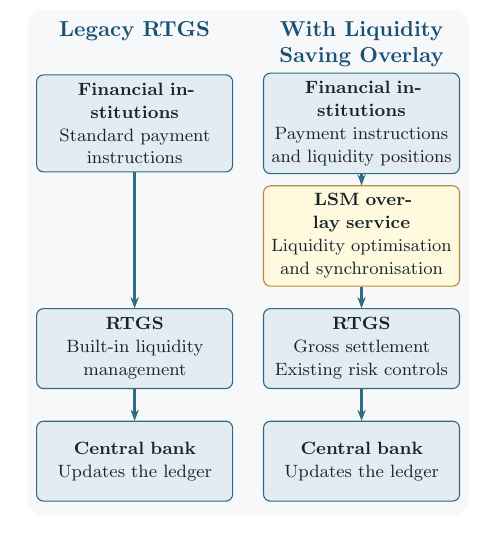
\begin{tikzpicture}[x=1cm,y=1cm,scale=.715,transform shape,
  orchbox/.style={rectangle,rounded corners=2.5pt,draw=Ocean,fill=lockfill,text=Ink,line width=.4pt,
    text width=3.20cm,minimum height=1.42cm,inner sep=4pt,align=center,font=\fontsize{9.5}{11.6}\selectfont},
  orchflow/.style={draw=Ocean,line width=.9pt,-{Stealth[length=4pt]}},
  orchheading/.style={anchor=north,inner sep=0pt,text=Rust,font=\fontsize{11.2}{13.4}\selectfont\bfseries}]
\path[use as bounding box] (0,0) rectangle (7.83,-8.54);
\fill[Soft!55!Paper,rounded corners=5pt] (0.00,0.32) rectangle (7.83,-8.66);
\node[orchheading] at (1.90,0.12) {Legacy RTGS};
\node[orchheading,align=center] at (5.93,0.12) {With Liquidity\\Saving Overlay};

\node[orchbox] (legacyfi) at (1.90,-1.70) {\textbf{Financial institutions}\\Standard payment\\instructions};
\node[orchbox] (legacyrtgs) at (1.90,-5.70) {\textbf{RTGS}\\Built-in liquidity\\management};
\node[orchbox] (legacycb) at (1.90,-7.70) {\textbf{Central bank}\\Updates the ledger};
\draw[orchflow] (legacyfi.south) -- (legacyrtgs.north);
\draw[orchflow] (legacyrtgs.south) -- (legacycb.north);

\node[orchbox] (overlayfi) at (5.93,-1.70) {\textbf{Financial institutions}\\Payment instructions\\and liquidity positions};
\node[orchbox,fill=deffill,draw=defline] (overlay) at (5.93,-3.70) {\textbf{LSM overlay service}\\Liquidity optimisation\\and synchronisation};
\node[orchbox] (overlayrtgs) at (5.93,-5.70) {\textbf{RTGS}\\Gross settlement\\Existing risk controls};
\node[orchbox] (overlaycb) at (5.93,-7.70) {\textbf{Central bank}\\Updates the ledger};
\draw[orchflow] (overlayfi.south) -- (overlay.north);
\draw[orchflow] (overlay.south) -- (overlayrtgs.north);
\draw[orchflow] (overlayrtgs.south) -- (overlaycb.north);
\end{tikzpicture}\hspace*{-.10cm}
\end{columns}
\vfill\par{\fontsize{5.5}{5.75}\selectfont\color{FootnoteBlue}\hypersetup{urlcolor=FootnoteBlue,linkcolor=FootnoteBlue}{\fontsize{5.5}{5.75}\selectfont \textbf{Fedwire} runs pure RTGS with daylight credit and no LSM. \textbf{Gridlock resolution} covers circle search (\textbf{SIC}), bilateral offset (\textbf{RITS} auto-offset and targeted bilateral offset) and multilateral offset (\textbf{Kronos2}, \textbf{Lynx}, \textbf{CHAPS}, \textbf{BOJ-NET} and \textbf{HKD CHATS}); \textbf{T2} dissolves its queues with optimisation algorithms aimed at the highest settlement volume for the least liquidity. \textbf{CHIPS} uses stable matching, a patented (now expired) balanced-release algorithm trading liquidity savings against settlement delay.}\par}\vspace*{1.38bp}
\end{frame}

% END orchestration-layer.tex


\begin{frame}{Resequence, net, route}
\vspace{-0.2em}
{\fontsize{7.0}{8.3}\selectfont\color{black} Where wholesale payments can settle or wait, \textbf{resequencing} allows substantial liquidity savings. RITS's queue offers \textbf{priority statuses} and \textbf{bilateral auto-offset} but no \textbf{multilateral offsetting algorithm} of the kind T2 (Eurosystem), CHAPS (UK), and Lynx (Canada) run. An orchestration layer that sequences an Australian dollar obligation, Swift's shared ledger, Canton's Global Synchronizer, or a central synchronisation operator for multilateral exchange, would also choose whether the obligation finally settles in RITS, or in another system --- and possibly another currency.\par}
\vspace{.34cm}
\centerline{\adjustbox{max width=\textwidth,max height=3.55cm}{%
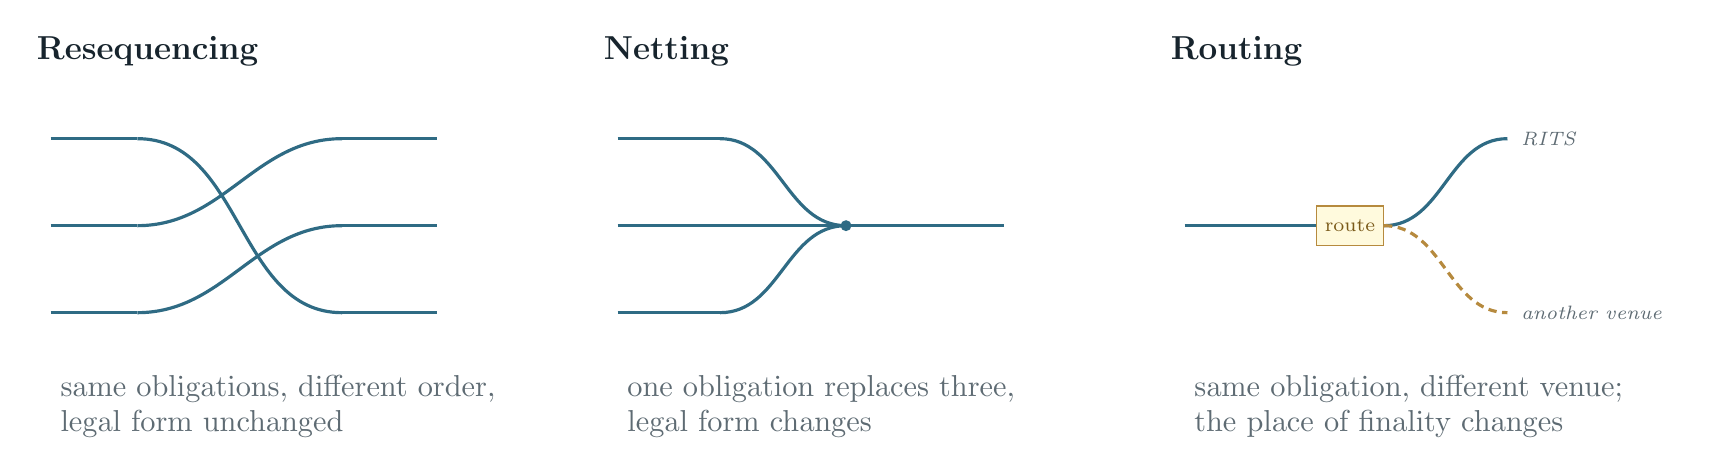
\begin{tikzpicture}[x=1cm,y=1.7cm,wire/.append style={line width=1.15pt},held/.append style={line width=1.15pt}]
% -resequence-
\begin{scope}[shift={(0,0)}]
\node[anchor=west,font=\large\bfseries,text=Ink] at (0,2.35) {Resequencing};
\foreach \y in {1.7,1.05,0.4}{\draw[wire] (0.3,\y) -- (1.4,\y);}
\draw[wire] (1.4,1.7) to[out=0,in=180] (4.0,0.4);
\draw[wire] (1.4,1.05) to[out=0,in=180] (4.0,1.7);
\draw[wire] (1.4,0.4) to[out=0,in=180] (4.0,1.05);
\foreach \y in {1.7,1.05,0.4}{\draw[wire] (4.0,\y) -- (5.2,\y);}
\node[nt,font=\fontsize{10.5}{12.6}\selectfont,text width=6.1cm,align=left] at (0.3,-0.3) {same obligations, different order,\\legal form unchanged};
\end{scope}
% -net-
\begin{scope}[shift={(7.2,0)}]
\node[anchor=west,font=\large\bfseries,text=Ink] at (0,2.35) {Netting};
\foreach \y in {1.7,1.05,0.4}{\draw[wire] (0.3,\y) -- (1.6,\y);}
\draw[wire] (1.6,1.7) to[out=0,in=180] (3.2,1.05);
\draw[wire] (1.6,1.05) -- (3.2,1.05);
\draw[wire] (1.6,0.4) to[out=0,in=180] (3.2,1.05);
\node[pt] at (3.2,1.05) {};
\draw[wire] (3.2,1.05) -- (5.2,1.05);
\node[nt,font=\fontsize{10.5}{12.6}\selectfont,text width=6.1cm,align=left] at (0.3,-0.3) {one obligation replaces three,\\legal form changes};
\end{scope}
% -route-
\begin{scope}[shift={(14.4,0)}]
\node[anchor=west,font=\large\bfseries,text=Ink] at (0,2.35) {Routing};
\node[hx] (R) at (2.4,1.05) {route};
\draw[wire] (0.3,1.05) -- (R.west);
\draw[wire] (R.east) to[out=0,in=180] (4.4,1.7);
\draw[held] (R.east) to[out=0,in=180] (4.4,0.4);
\node[wl,anchor=west] at (4.45,1.7) {RITS};
\node[wl,anchor=west] at (4.45,0.4) {another venue};
\node[nt,font=\fontsize{10.5}{12.6}\selectfont,text width=6.1cm,align=left] at (0.3,-0.3) {same obligation, different venue;\\the place of finality changes};
\end{scope}
\end{tikzpicture}}}
\vspace{.34cm}{\color{neutline}\hrule height .35pt}\vspace{.10cm}
{\fontsize{7.0}{8.3}\selectfont\color{black} RITS settles gross and real-time, but also runs multilateral group settlement for batch and retail payment systems. Once cross-border ledgers are interoperating, domestic AUD obligations between two Australian banks could potentially be routed over an orchestration layer to settle in external multi-currency systems that the RBA does not govern. As industry shifts to a tokenised financial system that operates 24/7 across global markets, the RBA must establish whether RITS will retain its exclusive legal designation for settlement finality over domestic interbank payments.\par}
\end{frame}





% Agorá slides (7 Oct 2026, author's request): two slides immediately before the RITS requirements.
{%
\newcommand{\labf}{\sffamily\bfseries\fontsize{6.9}{8.2}\selectfont}
\newcommand{\bodyf}{\sffamily\fontsize{6.4}{7.7}\selectfont}
\begin{frame}[t]{Project Agorá}
\hyphenpenalty=10000\exhyphenpenalty=10000
\begin{tikzpicture}[remember picture,overlay,x=1cm,y=-1cm,
  txt/.style={anchor=north west,inner sep=0pt,outer sep=0pt,align=left,text=Ink,execute at begin node={\raggedright\spaceskip=0pt\relax}},
  ledger/.style={rectangle,draw=lockline,fill=lockfill,line width=.4pt,anchor=north west,inner sep=0pt,outer sep=0pt},
  reserve/.style={rectangle,draw=Rust,fill=Rust!10!Paper,line width=.4pt,anchor=north west,inner sep=0pt,outer sep=0pt},
  strip/.style={rectangle,fill=Rust,anchor=north west,inner sep=0pt,outer sep=0pt},
  chip/.style={rectangle,draw=Rust,fill=Paper,text=Rust,line width=.35pt,inner xsep=2.5pt,inner ysep=1.5pt,font=\sffamily\fontsize{5.7}{6.5}\selectfont},
  cbchip/.style={rectangle,draw=Rust,fill=Rust!10!Paper,text=Ink,line width=.35pt,inner xsep=2.5pt,inner ysep=1.5pt,font=\sffamily\fontsize{5.7}{6.5}\selectfont},
  flow/.style={draw=Quiet,line width=.6pt,{Stealth[length=3.6pt,width=2.8pt]}-{Stealth[length=3.6pt,width=2.8pt]}},
  note/.style={font=\sffamily\itshape\fontsize{6.1}{7.1}\selectfont,text=Quiet,align=center,inner sep=1pt,fill=Paper}]
\begin{scope}[shift={(current page.north west)}]
\node[txt,align=justify,execute at begin node={},text width=14.76cm,font=\sffamily\fontsize{7.4}{8.8}\selectfont] at (.62,1.20)
  {\textbf{Correspondent banking} routes cross-border payments through chains of \textbf{nostro accounts}, resulting in delays, limited traceability, and prefunding requirements at each intermediary. These frictions contributed to the rapid adoption of payment stablecoins, including for card scheme settlement. The \textbf{Bank for International Settlements} and various central banks have undertaken research projects to test the use of tokenised central bank money to improve cross-currency settlement.\par\vspace{2pt}
  One of these projects, \textbf{Project mBridge} (2021--present) advanced to a \textbf{Minimum Viable Product} stage in 2024.\par\vspace{1pt}
  The mBridge architecture leaves no role for correspondent banking in cross-border PvP, with settlement made in central bank money on a ledger facilitating direct settlement in CBDC. Project Agor\'a, launched in 2024, retains correspondent banking arrangements: each central bank's money remains on its domestic ledger, while commercial bank money circulates on a shared international ledger.};
% ---- Generic jurisdictions: the same colours identify each issuer in both diagrams.
\definecolor{AgoraRed}{HTML}{C84A55}
\definecolor{AgoraGreen}{HTML}{26866C}
\definecolor{AgoraBlue}{HTML}{387FB5}
\definecolor{AgoraYellow}{HTML}{E4BC3B}
\definecolor{AgoraDepositPurple}{HTML}{8574BA}
\definecolor{AgoraDepositAmber}{HTML}{D3914C}
\definecolor{AgoraDepositPink}{HTML}{C875A6}
\begin{scope}[
  bank/.style={rectangle,rounded corners=1.5pt,line width=.55pt,
    minimum width=1.56cm,minimum height=.46cm,inner sep=1.3pt,outer sep=0pt,
    text=Ink,align=center,font=\sffamily\fontsize{6.9}{7.9}\selectfont},
  issue/.style={line width=.65pt,-{Stealth[length=3.5pt,width=2.9pt]}},
  token/.style={circle,minimum size=.28cm,inner sep=0pt,outer sep=0pt,
    text=Ink,font=\sffamily\bfseries\fontsize{5.6}{6.2}\selectfont},
  deposit/.style={regular polygon,regular polygon sides=3,minimum size=.22cm,
    inner sep=0pt,outer sep=0pt,line width=.45pt},
  local/.style={rectangle,rounded corners=1.5pt,line width=.55pt,
    minimum width=1.56cm,minimum height=1.02cm,inner xsep=1.3pt,inner ysep=1pt,
    outer sep=0pt,text=Ink,align=center,font=\sffamily\fontsize{6.0}{6.5}\selectfont},
  common/.style={rectangle,rounded corners=2pt,draw=Quiet!55,fill=Soft,
    line width=.55pt,inner sep=0pt,outer sep=0pt,anchor=north west},
  link/.style={line width=.65pt,densely dotted}]
\node[txt,text=Rust,font=\displayfont\bfseries\fontsize{7.6}{9.0}\selectfont] (mbtitle) at (.80,3.98) {mBridge: one shared platform};
\node[txt,text=Rust,font=\displayfont\bfseries\fontsize{7.6}{9.0}\selectfont] (agtitle) at (8.38,3.98) {Agorá: two layers};

% Current participating jurisdictions: Macao joined mBridge in 2026; Saudi Arabia left in 2025.
% Sources: https://www.gsef.gov.mo/pt/posts/11809 and SAMA's September 2026 statement.
\node[anchor=west,inner sep=0pt,outer sep=0pt,font=\sffamily\fontsize{7.6}{8.4}\selectfont] at ([xshift=.20cm]mbtitle.east) {\flag{china}\hspace{.15em}\flag{hong-kong}\hspace{.15em}\flag{thailand}\hspace{.15em}\flag{united-arab-emirates}\hspace{.15em}\flag{macao}};
% Eurosystem represented by Banque de France; Canada joined Agorá in May 2026.
% Source: https://www.bankofcanada.ca/2026/05/bank-canada-joins-bis-project-agora-test-improvements-wholesale-cross-border-payments/
\node[anchor=west,inner sep=0pt,outer sep=0pt,font=\sffamily\fontsize{7.6}{8.4}\selectfont] at ([xshift=.20cm]agtitle.east) {\flag{eu}\hspace{.15em}\flag{japan}\hspace{.15em}\flag{south-korea}\hspace{.15em}\flag{mexico}\hspace{.15em}\flag{switzerland}\hspace{.15em}\flag{united-kingdom}\hspace{.15em}\flag{united-states}\hspace{.15em}\flag{canada}};

% mBridge: all four central banks issue wholesale CBDC on one ledger.
\node[common,minimum width=6.72cm,minimum height=1.25cm] at (.85,5.30) {};
\foreach \x/\id/\col in {1.62/A/AgoraRed,3.34/B/AgoraGreen,5.06/C/AgoraBlue,6.78/D/AgoraYellow}{
  \node[bank,draw=\col!60!black,fill=\col!60!black,text=Paper] (mb\id) at (\x,4.65) {Central bank \id};
  \draw[issue,draw=\col] (mb\id.south) -- (\x,5.30);
  \node[token,draw=\col,fill=\col!80!Paper] at (\x,5.72) {\id};
}
\node[font=\sffamily\itshape\fontsize{6.5}{7.5}\selectfont,text=Quiet,fill=Paper,inner sep=1.5pt] at (4.20,5.13) {issue wCBDC};
\node[font=\sffamily\bfseries\fontsize{7.6}{8.8}\selectfont,text=Rust,inner sep=0pt] at (4.21,6.27) {mBridge Ledger};

% mBridge FX workflow, using the approved summary of the published payment flow.
\node[strip,minimum width=6.72cm,minimum height=.50cm] at (.85,6.70) {};
\node[anchor=center,align=center,text=Paper,inner sep=0pt,font=\sffamily\fontsize{6.1}{7.0}\selectfont] at (4.21,6.95) {Agree counterparties and FX terms $\rightarrow$ bank checks and confirmation\\$\rightarrow$ \textbf{commit} $\rightarrow$ \textbf{atomic PvP settlement}};

% Agorá: each reserve ledger remains local; the shared ledger carries deposits.
\foreach \x/\id/\col/\depone/\deptwo in {9.18/A/AgoraRed/AgoraDepositPurple/AgoraDepositAmber,10.92/B/AgoraGreen/AgoraDepositPink/AgoraDepositPurple,12.66/C/AgoraBlue/AgoraDepositAmber/AgoraDepositPink,14.40/D/AgoraYellow/AgoraDepositPurple/AgoraDepositPink}{
  \node[bank,draw=\col!60!black,fill=\col!60!black,text=Paper] (agcb\id) at (\x,4.65) {Central bank \id};
  \node[local,draw=\col,fill=\col!12!Paper] (aglocal\id) at (\x,5.67) {};
  \node[font=\sffamily\bfseries\fontsize{6.5}{7.4}\selectfont,text=Ink,inner sep=0pt] at (\x,5.38) {Local ledger \id};
  \node[token,draw=\col,fill=\col!80!Paper] at ({\x-.43},5.83) {\id};
  \node[deposit,draw=\depone!80!black,fill=\depone!80!Paper] at (\x,5.83) {};
  \node[deposit,draw=\deptwo!80!black,fill=\deptwo!80!Paper] at ({\x+.43},5.83) {};
  \draw[issue,draw=\col] (agcb\id.south) -- (aglocal\id.north);
  \draw[link,draw=\col] (aglocal\id.south) -- (\x,6.35);
}
\node[common,minimum width=6.82cm,minimum height=.40cm] at (8.38,6.35) {};
\foreach \x/\col in {8.87/AgoraDepositPurple,9.37/AgoraDepositAmber,14.19/AgoraDepositPink,14.69/AgoraDepositPurple}{
  \node[deposit,draw=\col!80!black,fill=\col!80!Paper] at (\x,6.55) {};
}
\node[font=\sffamily\fontsize{7.2}{8.2}\selectfont,text=Rust,inner sep=0pt] at (11.79,6.55) {\textbf{Unifying ledger}\quad Tokenised deposits};
\node[strip,minimum width=6.82cm,minimum height=.30cm] at (8.38,6.90) {};
\node[anchor=center,text=Paper,inner sep=0pt,font=\sffamily\fontsize{6.0}{7.0}\selectfont] at (11.79,7.05) {confirm payee $\rightarrow$ path $\rightarrow$ validate $\rightarrow$ \textbf{lock} $\rightarrow$ \textbf{settle}: commit or cancel};
% Shared symbol key: central-bank money uses circles; commercial-bank deposits use triangles.
\node[anchor=east,inner sep=0pt,outer sep=0pt,text=black,font=\sffamily\fontsize{5.8}{6.8}\selectfont] (agdepositkey) at (15.38,8.66) {Tokenised deposit (CoBM)};
\node[deposit,draw=black,fill=black] (agdepositkeysymbol) at ([xshift=-.22cm]agdepositkey.west) {};
\node[anchor=east,inner sep=0pt,outer sep=0pt,text=black,font=\sffamily\fontsize{5.8}{6.8}\selectfont] (agreservekey) at ([xshift=-.35cm]agdepositkeysymbol.west) {Tokenised CeBM/CBDC};
\node[token,minimum size=.24cm,draw=black,fill=black] at ([xshift=-.22cm]agreservekey.west) {};
\end{scope}
% ---- Illustrative cross-currency payments between the generic jurisdictions.
\begingroup\hypersetup{urlcolor=Quiet,linkcolor=Quiet}
\node[txt,text=Quiet,text width=6.94cm,font=\sffamily\itshape\fontsize{5.8}{6.8}\selectfont] at (.80,7.42) {\href{https://www.hkma.gov.hk/media/eng/doc/key-information/press-release/2022/20221026e3a1.pdf}{\textbf{A buyer in A pays a seller in B.}} The buyer's bank debits its customer's deposit and sends A's CBDC to the seller's bank, which credits the seller's deposit. The receiving bank can hold, reuse, or exchange that CBDC. If the seller wants B's currency, a bank supplies FX: the two CBDCs can be exchanged atomically through PvP.};
\node[txt,text=Quiet,text width=6.94cm,font=\sffamily\itshape\fontsize{5.8}{6.8}\selectfont] at (8.38,7.42) {\href{https://www.bis.org/project/agora}{\textbf{A buyer in A pays a seller in B.}} Banks and correspondents agree the route and FX amounts, validate the payment, and lock balances. Customer and correspondent deposits change on the unifying ledger; reserves move on domestic ledgers. All legs follow one commit-or-cancel decision. The seller receives a deposit in the agreed currency.};
\endgroup
\end{scope}
\end{tikzpicture}
\end{frame}

\newcommand{\agnum}[1]{\tikz[baseline=(agn.base)]{\node[circle,fill=Rust,text=white,font=\bfseries\fontsize{6.0}{6.0}\selectfont,inner sep=0pt,minimum size=.34cm] (agn) {#1};}}
\newcommand{\agreq}[3]{\par\noindent\hangindent=.38cm\hangafter=1\makebox[.38cm][l]{\raisebox{0pt}[0pt][0pt]{\agnum{#1}}}{\bfseries\color{Rust}#2}\enspace #3\par}
\begin{frame}[t]{Agorá: Jurisdictional Ledger requirements}
\hyphenpenalty=10000\exhyphenpenalty=10000
\begin{tikzpicture}[remember picture,overlay,x=1cm,y=-1cm,
  reqtxt/.style={anchor=north west,inner sep=0pt,outer sep=0pt,align=left,text=Ink}]
\begin{scope}[shift={(current page.north west)}]
\node[reqtxt,text width=14.76cm,font=\sffamily\fontsize{7.1}{8.6}\selectfont] at (.62,1.20) {\href{https://www.bis.org/publications/project-agora-shared-programmable-platform-wholesale-cross-border-payments.pdf}{The Agor\'a report sets out fifteen business requirements.} Each leaves scope for a variety of implementations.};
\node[reqtxt] at (.62,1.86) {\begin{minipage}[t][6.76cm][t]{7.90cm}
\sffamily\fontsize{7.2}{8.4}\selectfont\raggedright\setlength{\parskip}{0pt}
\agreq{1}{Jurisdictional autonomy and governance.}{Central banks retain control of reserves, monetary policy, participation, and domestic operations.}
\vfill
\agreq{2}{Issuance, redemption, and transfer.}{Preserve legal claims and balance sheets, with auditable movements and exceptional issuer controls.}
\vfill
\agreq{3}{Atomic settlement of every leg.}{All legs succeed or fail together, across currencies and ledgers.}
\vfill
\agreq{4}{Pathfinding and identification.}{Agree eligible routes and verify correspondent links, respecting each bank's routing rules.}
\vfill
\agreq{5}{Cross-currency integrity.}{Apply agreed currency amounts consistently across every payment leg.}
\vfill
\agreq{6}{Access, participation, and authorisation.}{Define token access and limit delegated actions; originating participants remain accountable.}
\vfill
\agreq{7}{Compliance pre-validation and screening.}{Settle only after each bank's sanctions, AML/CFT, fraud, and balance checks pass.}
\vfill
\agreq{8}{\href{https://www.bis.org/cpmi/publ/d230.pdf}{ISO 20022 data standards, quality, and interoperability.}}{Preserve payment data across systems; validate identifiers, amounts, and required fields.}
\vfill
\agreq{9}{Reduction of exceptions and investigations.}{Use early checks, clear responsibilities, timeouts, and unambiguous cancellation outcomes.}
\vfill
\agreq{10}{Transparency, notifications, and reporting.}{Give authorised participants timely status, confirmations, balances, and audit trails.}
\end{minipage}};
\node[reqtxt] at (8.88,1.86) {\begin{minipage}[t][3.94cm][t]{6.50cm}
\sffamily\fontsize{7.2}{8.4}\selectfont\raggedright\setlength{\parskip}{0pt}
\agreq{11}{Privacy and selective data-sharing.}{Share only necessary data with authorised participants, within local rules.}
\vfill
\agreq{12}{Liquidity management and monitoring.}{Track reserve and deposit balances across currencies, 24/7.}
\vfill
\agreq{13}{Governance and allocation of roles and responsibilities.}{Institutions retain customer servicing, compliance, and reconciliation duties.}
\vfill
\agreq{14}{\href{https://www.bis.org/committees/cpmi/pfmi/overview}{Platform reliability, security, and scalability.}}{Meet measurable performance and availability standards, with predictable recovery from outages.}
\vfill
\agreq{15}{A clearly defined settlement-finality trigger.}{Define a legally enforceable finality point across jurisdictions, including in insolvency.}
\end{minipage}};
% Swift's role and ledger response: facts linked to primary sources; competitive threat is an inference.
\filldraw[fill=DesignGrey!50!white,draw=black!35,line width=.35pt] (8.88,5.99) rectangle (15.38,8.64);
\node[reqtxt,anchor=north,text=black!60,font=\displayfont\bfseries\fontsize{7.0}{8.4}\selectfont] at (12.13,6.16) {The Swift Ledger};
\node[reqtxt,text width=6.06cm,font=\sffamily\fontsize{5.9}{6.9}\selectfont] at (9.10,6.58) {\raggedright
\href{https://www.swift.com/about-us/who-we-are/what-swift}{Swift is the messaging network underpinning correspondent banking.} Direct cross-border CBDC settlement would bypass this network, but \href{https://www.bis.org/publications/project-agora-shared-programmable-platform-wholesale-cross-border-payments.pdf}{Agorá preserves its role}, positioning Swift as a natural vendor to supply its unified ledger.\par\vspace{3pt}
\href{https://www.swift.com/insights/news/swift-add-blockchain-based-ledger}{Swift announced its ledger in September 2025}, during Agorá's prototype development. \href{https://www.bis.org/publications/project-agora-shared-programmable-platform-wholesale-cross-border-payments.pdf}{Both use \textbf{Hyperledger Besu}}. \href{https://www.swift.com/insights/news/swifts-blockchain-based-shared-ledger-progresses-mvp-implementation}{Swift calls it a ``shared digital orchestration layer'': coordinating payment commitments while \emph{final} settlement uses existing systems.}};
\end{scope}
\end{tikzpicture}
\end{frame}

}

\begin{frame}[t]{Tokenised reserves: RITS requirements}
\setbeamerfont{itemize/enumerate body}{size=\fontsize{8.0}{10.0}}\fontsize{8.0}{10.0}\selectfont
\vspace{-0.1em}
  \vspace{0pt plus 0.35fill}\begin{itemize}\setlength{\itemsep}{2pt plus 2.4fill}
    \item \rust{wCBDC vs ``tokenised CeBM''.} A digital twin can represent an ESA balance. That balance must sit in an account that cannot be spent through RITS while tokens are outstanding. Every mint or burn must be matched by a transfer into or out of it, so token supply and balance stay equal. A native token (wholesale CBDC) would be a direct RBA liability, and require its own legal basis for finality, as the RITS Regulations give ESA movements today.
    \item \rust{Agor\'a compatibility.} A jurisdictional reserve ledger under the RBA's own authority, carrying tokenised ESA balances rather than a wCBDC, with locking, cross-domain coordination, embedded compliance, and finality under Australian law.
    \item \rust{Public or private ledger operator.} An RBA-run ledger means every external platform still synchronises to it; a third-party ledger requires enforceable observation, access, governance and recovery rights, as well as clear issuer control. Any private operator would need to be domestic, credibly neutral, and user-owned; AP+ or a national industry consortium of a similar type.
    \item \rust{Hours of operation.} Continuous circulation against business-hours issuance and redemption opens a conversion constraint between two RBA liabilities. The Pontes plan for continuous operation in 2028 requires tokens to remain outstanding outside T2 hours, with finality moved from T2 onto the Eurosystem's own DLT platform.
    \item \rust{Intraday credit on the ledger.} Settling every payment in full requires each bank to hold its peak gross position on the ledger. RITS meets this need by intraday repo during business hours. A 24/7 ledger warrants a similar type of facility, with programmable money and assets broadening the range of possible mechanism designs.
  \end{itemize}\vspace{0pt plus 4fill}
\end{frame}
\fi

% Recommendations are incorporated into Area 4 submission responses and requirements.



% Project Agora section-title slide deleted 6 October 2026 at the author's request.

% BEGIN agora-summary.tex
% The "Project Agorá" and "A national ledger for the Australian dollar" slides moved to applus-impact-deck.tex on 6 October 2026.
% END agora-summary.tex

% The "dominant issuer's token" slide moved to rits-extras.tex on 6 October 2026.


% The Australian Payments Plus Impact Analysis section moved to applus-impact-deck.tex on 6 October 2026.




% BEGIN submission-responses.tex -- generated from recommendatiosn.docx, 6 October 2026

\definecolor{ResponseBlue}{HTML}{E8EDF1}

{\setbeamercolor{background canvas}{bg=Rust}\begin{frame}[plain]\vfill\centering
{\color{white}\displayfont\fontsize{24.5}{27.4}\selectfont\bfseries Submission responses\par}
\vspace{.42cm}{\color{Mist}\fontsize{8.0}{9.6}\selectfont which do \textbf{not} represent the positions or policies of any organisation\par}\vfill\end{frame}}


% Restyled 6-7 Oct 2026: top stripe with a short header per answer; type size fitted per page so the boxes fill it.
\newsavebox{\RespBoxA}\newsavebox{\RespBoxB}\newsavebox{\RespBoxC}
\newcommand{\respsize}{7.6}\newcommand{\resplead}{8.8}
\newcommand{\responsetext}[2][\raggedright]{\begin{minipage}{13.76cm}#1\hyphenpenalty=10000\exhyphenpenalty=10000\fontsize{\respsize}{\resplead}\selectfont\color{Ink}\setlength{\parindent}{0pt}#2\end{minipage}}
\newcommand{\responsejustified}[1]{\responsetext[\leftskip=0pt\rightskip=0pt\parfillskip=0pt plus 1fil\relax]{#1}}
\newcommand{\respTarget}{7.6}
\newcommand{\respPairTop}{1.30}\newcommand{\respPairGap}{.62}\newcommand{\respPairHeight}{7.08}
\newcommand{\responsebox}[5]{% #1 top y, #2 bottom y, #3 Q label, #4 header, #5 savebox
  \fill[White] (.62,#1) rectangle (15.38,#2);
  \fill[Rust] (.62,#1) rectangle (15.38,#1-.44);
  \draw[Rust,line width=.5pt] (.62,#1) rectangle (15.38,#2);
  \node[anchor=west,inner sep=0pt,text=White,font=\displayfont\fontsize{7.4}{8.8}\selectfont\bfseries] at (.82,#1-.22) {#3\enspace\textperiodcentered\enspace #4};
  \node[anchor=west,inner sep=0pt] at (1.12,{((#1-.44)+(#2))/2}) {\usebox{#5}};}
\newcommand{\responseboxtight}[5]{% as \responsebox, with .14 cm inner padding (three-answer page)
  \fill[White] (.62,#1) rectangle (15.38,#2);
  \fill[Rust] (.62,#1) rectangle (15.38,#1-.44);
  \draw[Rust,line width=.5pt] (.62,#1) rectangle (15.38,#2);
  \node[anchor=west,inner sep=0pt,text=White,font=\displayfont\fontsize{7.4}{8.8}\selectfont\bfseries] at (.82,#1-.22) {#3\enspace\textperiodcentered\enspace #4};
  \node[anchor=west,inner sep=0pt] at (1.12,{((#1-.44)+(#2))/2}) {\usebox{#5}};}
\newcommand{\responsepair}[7]{% title, Qa, headerA, textA, Qb, headerB, textB
{\setbeamercolor{background canvas}{bg=ResponseBlue}\setbeamercolor{frametitle}{bg=ResponseBlue,fg=Rust}%
\setbeamerfont{frametitle}{size=\fontsize{12.4}{14.8},series=\bfseries}%
\begin{frame}[t]{#1}
% Use a common target (\respTarget, 7.6pt unless a page sets otherwise); compact only dense responses in 0.1pt steps.
\let\respsize\respTarget\pgfmathsetmacro{\resplead}{\respsize*1.22}%
\loop
  \sbox{\RespBoxA}{\responsetext{#4}}\sbox{\RespBoxB}{\responsetext{#7}}%
  \pgfmathsetmacro{\hA}{(\the\ht\RespBoxA+\the\dp\RespBoxA)/28.45274}%
  \pgfmathsetmacro{\hB}{(\the\ht\RespBoxB+\the\dp\RespBoxB)/28.45274}%
  \pgfmathsetmacro{\nA}{.44+.22+\hA+.22}\pgfmathsetmacro{\nB}{.44+.22+\hB+.22}%
  \pgfmathsetmacro{\respTotal}{\nA+\nB+\respPairGap}%
  \pgfmathtruncatemacro{\respGo}{(\respTotal>\respPairHeight)&&(\respsize>6.0)}%
\ifnum\respGo=1
  \pgfmathsetmacro{\respsize}{\respsize-0.1}\pgfmathsetmacro{\resplead}{\respsize*1.22}%
\repeat
\sbox{\RespBoxA}{\responsejustified{#4}}\sbox{\RespBoxB}{\responsejustified{#7}}%
\typeout{RESPFIT pair #1: size=\respsize total=\respTotal}\pgfmathsetmacro{\respExtra}{max(\respPairHeight-\respTotal,0)/2}%
\pgfmathsetmacro{\yAbot}{-\respPairTop-\nA-\respExtra}\pgfmathsetmacro{\yBtop}{\yAbot-\respPairGap}\pgfmathsetmacro{\yBbot}{\yBtop-\nB-\respExtra}%
\begin{tikzpicture}[remember picture,overlay,x=1cm,y=1cm]
\begin{scope}[shift={(current page.north west)}]
\responsebox{-\respPairTop}{\yAbot}{#2}{#3}{\RespBoxA}
\responsebox{\yBtop}{\yBbot}{#5}{#6}{\RespBoxB}
\end{scope}
\end{tikzpicture}
\end{frame}}}
\newcommand{\responsetriple}[9]{% title, Qa, hA, tA, Qb, hB, tB, Qc, hC; the third text follows as a tenth brace group
\def\rtTitle{#1}\def\rtQa{#2}\def\rtHa{#3}\def\rtTa{#4}\def\rtQb{#5}\def\rtHb{#6}\def\rtTb{#7}\def\rtQc{#8}\def\rtHc{#9}%
\responsetriplecont}
\newcommand{\responsetriplecont}[1]{%
\def\rtTc{#1}%
{\setbeamercolor{background canvas}{bg=ResponseBlue}\setbeamercolor{frametitle}{bg=ResponseBlue,fg=Rust}%
\setbeamerfont{frametitle}{size=\fontsize{12.4}{14.8},series=\bfseries}%
\begin{frame}[t]{\rtTitle}
\let\respsize\respTarget\pgfmathsetmacro{\resplead}{\respsize*1.22}%
\loop
  \sbox{\RespBoxA}{\responsejustified{\rtTa}}\sbox{\RespBoxB}{\responsejustified{\rtTb}}\sbox{\RespBoxC}{\responsejustified{\rtTc}}% measured as rendered (8 Oct 2026)
  \pgfmathsetmacro{\hA}{(\the\ht\RespBoxA+\the\dp\RespBoxA)/28.45274}%
  \pgfmathsetmacro{\hB}{(\the\ht\RespBoxB+\the\dp\RespBoxB)/28.45274}%
  \pgfmathsetmacro{\hC}{(\the\ht\RespBoxC+\the\dp\RespBoxC)/28.45274}%
  \pgfmathsetmacro{\nA}{.44+.14+\hA+.14}\pgfmathsetmacro{\nB}{.44+.14+\hB+.14}\pgfmathsetmacro{\nC}{.44+.14+\hC+.14}%
  \pgfmathsetmacro{\respTotal}{\nA+\nB+\nC+.56}%
  \pgfmathtruncatemacro{\respGo}{(\respTotal>7.43)&&(\respsize>6.0)}%
\ifnum\respGo=1
  \pgfmathsetmacro{\respsize}{\respsize-0.1}\pgfmathsetmacro{\resplead}{\respsize*1.22}%
\repeat
\sbox{\RespBoxA}{\responsejustified{\rtTa}}\sbox{\RespBoxB}{\responsejustified{\rtTb}}\sbox{\RespBoxC}{\responsejustified{\rtTc}}%
\typeout{RESPFIT triple: size=\respsize total=\respTotal}\pgfmathsetmacro{\respExtra}{max(7.43-\respTotal,0)/3}%
\pgfmathsetmacro{\yAbot}{-1.12-\nA-\respExtra}\pgfmathsetmacro{\yBtop}{\yAbot-.28}\pgfmathsetmacro{\yBbot}{\yBtop-\nB-\respExtra}%
\pgfmathsetmacro{\yCtop}{\yBbot-.28}\pgfmathsetmacro{\yCbot}{\yCtop-\nC-\respExtra}%
\begin{tikzpicture}[remember picture,overlay,x=1cm,y=1cm]
\begin{scope}[shift={(current page.north west)}]
\responseboxtight{-1.12}{\yAbot}{\rtQa}{\rtHa}{\RespBoxA}
\responseboxtight{\yBtop}{\yBbot}{\rtQb}{\rtHb}{\RespBoxB}
\responseboxtight{\yCtop}{\yCbot}{\rtQc}{\rtHc}{\RespBoxC}
\end{scope}
\end{tikzpicture}
\end{frame}}}

\responsepair{Area 1: Synchronisation}{Q1}{Synchronisation models}{RITS should be capable of supporting central bank \textbf{reserves lock 24/7}. While RITS cannot lock reserves on an external platform it doesn't control, it should be able to interface with external platforms through a \textbf{ISO20022-based API} that supports DvP with asset-locking on those platforms. The API should offer \textbf{asset-lock, reserves-lock or dual-lock DvP/PvP} support, accommodating counterparty preferences for any potential asset transaction (e.g. real-estate, securities, FX) settled under a future national payments scheme.\par\vspace{5pt} FSS is the prefunded retail support that operates during RITS ``after hours'', without support for reservation locking. FSS could be upgraded to support locks, DvP, synchronization, and wholesale payments; in doing so, the enhanced FSS would effectively become the \textbf{main settlement engine}; so RITS would operate 24/7 `normally'.}{Q2}{Synchronisation arrangements}{The RBA should provide an interface to central bank reserves for third-party operators including \textbf{Australian Payments Plus} as user-owned operator of an interbank AUD settlement facility synchronizing RITS with programmable asset platforms. The utility would be governed by an industry scheme under regulatory oversight, guaranteeing \textbf{PSNA finality} on both payment and asset side. The utility should support AUD deposit token interchange and DvP/PvP settlement, including \textbf{T2S-style auto-collateralization}, using ISO20022.\par\vspace{5pt} This interface would be consistent with the requirements of the \textbf{BIS \textbf{Agora framework}} for maintaining a two-tier international monetary system.}

\responsepair{Area 1: Synchronisation \textit{(continued)}}{Q3}{Existing RITS and FSS capabilities}{RITS supports asset-lock links (Austraclear, CHESS) and reserves-lock batches (PEXA, Sympli), but only during business hours. FSS settles continuously, but has no reservation service. RITS feeder systems lack a common API, and there is no service for \textbf{credit-within-settlement} (which would enable \textbf{auto-collateralisation}). PayTo authorization cannot reserve ESA funds, and the NPP cannot support settlement synchronization in its current form.\par\vspace{5pt} An upgrade of the FSS to support reservation locks and 24/7 synchronized real-time settlement outside of the NPP will likely adversely affect the valuation of existing NPPA assets -- but AP+ recognizes that the RBA will correctly disregard \textbf{existing payment infrastructures' sunk costs} when evaluating available options for RITS modernization.}{Q4}{Required enhancements}{The RBA should add \textbf{24/7 reservation functionality} and a \textbf{standardised ISO 20022 API} for settlement use cases, modeled on the Eurosystem T2S/TIPS. The RBA should clarify the extent of \textbf{RBA liquidity facility} support for continuous settlement in wholesale asset markets, and explore credit against purchased or pledged assets, including T2S-style \textbf{auto-collateralisation}.\par\vspace{5pt} This would support a new market in intraday liquidity, but would require integration between a modernized RITS and a modernized ASX Austraclear (or equivalent).}

\def\respTarget{8.2}% Area 2 pages one size larger (7 Oct 2026)
\responsepair{Area 2: At-par exchange}{Q5}{Exchange models}{RITS/FSS should support a national deposit token network with a 24/7 \textbf{multilateral mint--burn facility} synchronized to reserved ESA funds in RITS. The lock would reserve issuer A's payment to B while A's token is burned and B's token is minted; the reservation would then be released to settle.\par\vspace{5pt} A scheme facility would limit par interchange to a common instrument type: \textbf{deposit tokens}. Because stablecoins maintain par under different legal arrangements and without access to RBA liquidity, a RITS synchroniser should not be used to ``peg'' them to Basel-regulated deposits.}{Q6}{Synchronisation arrangements for exchange}{Exchange models should receive the same service for central bank supported interbank payment settlement as conventional account-to-account payments (i.e. HVCS, BECS or NPP), under the same types of rules. The RBA could provide the facility to the deposit token network directly (as in the Bank of Korea's \textbf{Project Hangang}), or a synchronizer could link an external facility (e.g. an AP+ token interchange) to RITS under the \textbf{accredited operator class}. Operators pre-processing payments for settlement would require infrastructure supervision, finality, loss allocation and recovery rules.}

{\def\respTarget{9.0}% At-par exchange (continued) only: larger text (7 Oct 2026)
\responsepair{Area 2: At-par exchange \textit{(continued)}}{Q7}{Existing capabilities for exchange}{The existing RITS/FSS could not support an effective reserve-collateralised \textbf{multilateral mint--burn facility} as RITS main operating hours are limited, the FSS lacks reservation functionality, and both lack an API.}{Q8}{Required enhancements}{Enhancements should include continuous reservation, redemption and -- either directly or through an industry consortium, or operator -- a common mint--burn service for AUD \textbf{deposit tokens}. Longer term, establish an API for a multi-issuer AUD intraday settlement token direct the formation of a \textbf{national industry scheme} for multi-issuer AUD intraday settlement.\par\vspace{5pt} ESA holders (and potentially non-holders) could mint and burn this token on demand against pooled tokenised HQLA, programmed according to the RBA's rulebook on \textbf{repo-eligible collateral}. This would improve access to secured intraday credit and contribute to AUD monetary singleness without requiring a new digital form of RBA liability or a reliance on a centralized mint-burn interchange.}}

\def\respTarget{7.6}
\responsetriple{Area 3: Reserve access}{Q9}{Use of reserve access}{Stablecoins should not be generally interchangeable for \textbf{deposit tokens} within a single token interchange facility, due to the substantive differences in the legal character of the instruments and their regulatory regimes. The RBA -- through the \textbf{Deposit Token Working Group} -- must clearly establish the role of AUD-denominated central bank money in deposit token interchange to differentiate them from stablecoins, both in wholesale and retail context -- cf the role taken by the Bank of Korea in the \textbf{Project Hangang} deposit token network.\par\vspace{2pt} For stablecoins, a synchronization operator could lock ESA reserves for settlement and redemption, or for minting a fully reserves- collateralized token; an RBDC (or ``\textbf{synthetic CBDC}''). Industry adoption of a fully reserves-collateralised stablecoin (RBDC) as a multilateral deposit token settlement asset would represent an effective privatisation of the RBA's core central banking function. Other forms of stablecoin may be minted or redeemed against eligible collateral backing held by trusted register according to an RBA rulebook.}{Q10}{Account features}{Issuers require support for continuous issuance, redemption, and settlement access. RITS/FSS reservation functionality with legal segregation and holder rights is a basic requirement for synchronised interchange. With these features, a scheme-governed open-mint AUD (or ``\textbf{AUD+}'') stablecoin could be maintained for on-demand tokenized settlement liquidity, based on an RBA rulebook and a trusted registry able to support locked par-value HQLA collateral.}{Q11}{Barriers beyond eligibility}{Unsegregated backing and liquidity constraints may obstruct stablecoin redemption into central bank reserves, causing their par to depeg. The RBA should develop a policy that would allow regulated stablecoin issuers to access a new, specialized \textbf{RBA liquidity facility} that could offer intraday credit for settlement finality against issuer's locked, \textbf{repo-eligible collateral} -- c.f.\ the recent Bank of England proposal for regulated stablecoins.}

{\def\respPairTop{1.10}\def\respPairGap{.36}\def\respPairHeight{7.52}\def\respTarget{7.6}
\responsepair{Area 4: Tokenised reserves}{Q12}{Use cases for tokenised reserves}{Tokenised reserves refers either to wCBDC or to what the ECB describes as ``\textbf{tokenized Central Bank Money}'';technically not wCBDC because these tokens ``wrap'' ESA balances -- being therefore the central bank liability's \textbf{digital twin} rather than the liability itself. Tokenised reserves would be created to settle transactions atomically on a common ledger with tokenized assets.\par\vspace{5pt} This ledger with tokenized reserves could be operated by the central bank under the \textbf{ECB Pontes model}, or by a trusted third party under the \textbf{Swiss Helvetica model}, but would only benefit use cases where tokenized assets are natively maintained on this same trusted platform and thereby able to settle atomically with legal finality. Where the tokenized asset settles against any other money token or synchronizer, the tokenized reserve adds no special benefit but introduces the complication of multiple liquidity pools.\par\vspace{5pt} In the short term, a fully-featured RITS synchronization operator facility with appropriate finality designation should be able to deliver programmability, operating hours and liquidity efficiency for most practical use cases.}{Q13}{Functional outcomes}{A tokenised reserve design should support \textbf{atomic settlement}, smart contracts, collateralised funding, continuous liquidity management, and external connections that allow heterogenous asset tokens to be minted on the ledger with legal effect. This multi-asset programmable ledger would be maintained either by the RBA (on the Eurosystem model) or by a trusted national industry user-owned operator (such as AP+, on the Swiss model). National scheme rules would define the authoritative delivery record and govern cross-platform transaction recovery.}}


\responsepair{Area 4: Tokenised reserves \textit{(continued)}}{Q14}{Issuance and distribution}{The ideal model would involve a ``\textbf{jurisdictional ledger}'' maintained on an open-source platform (e.g. \textbf{Hyperledger Besu}), owned and operated either by the RBA or by a national industry consortium (i.e. AP+) under RBA oversight, able to support same-ledger \textbf{atomic settlement} between wholesale tokenized reserves and heterogenous tokenised assets -- potentially including natively minted Australian Government Securities. This hypothetical ledger -- which could effectively function as a \textbf{multi-asset RITS-Austraclear-DLT} -- would be consistent with the \textbf{Agora framework} for maintaining an international system of two-tiered money.}{Q15}{Funding, redemption, and liquidity}{Conversion between ESA balances and tokenised reserves is unnecessary where the tokenised reserves are ``\textbf{digital twin}s'' (i.e. ESAs are locked against circulating tokens). The RBA should directly issue tokens against these locked reserves rather than encourage RBDC issuance. The RBA would issue tokenised reserves against locked reserves (as per Agora), avoiding the liquidity fragmentation that could result from ``real'' wCBDC being sold for reserves in the manner of physical currency. Funding, redemption, and liquidity-management concerns arise where operating hours of systems differ, recommended extended operating hours for the main RITS settlement engine. Funding must be accessible across systems to avoid fragmenting liquidity in separate reserve pools.}

% END submission-responses.tex


% AP+ impact assessment slides, added 7 October 2026 at the author's request.
% Copied verbatim from applus-four-deck.tex (lines 231-569 of that file); kept in its
% own group so the AP+ purple palette does not leak into the appendix.
\begingroup
\definecolor{APLavender}{HTML}{CDB9E4}
\definecolor{APDark}{HTML}{4B3268}
\definecolor{APPale}{HTML}{F4EFF8}
\definecolor{APMid}{HTML}{80639E}
\setbeamercolor{frametitle}{fg=Ink,bg=Paper}
\hypersetup{urlcolor=Rust,linkcolor=Rust}
\arrayrulecolor{BoxGrey}
% Title slide, matching applus-impact-deck.tex (added 7 Oct 2026 at the author's request).
{\setbeamercolor{background canvas}{bg=APDark}
\begin{frame}[plain]\vfill\centering
{\color{White}\displayfont\fontsize{24.5}{27.4}\selectfont\bfseries Australian Payments Plus\\Impact Assessment\par}\vfill
\end{frame}}


% All wording is retained from the current inline section.
\tikzset{
  aphead/.style={anchor=north west,inner sep=0pt,align=left,text=Rust,font=\displayfont\bfseries\fontsize{9.0}{10.8}\selectfont},
  apbody/.style={anchor=north west,inner sep=0pt,align=left,text=Ink,font=\fontsize{8.3}{10.3}\selectfont},
  apintro/.style={apbody,font=\bfseries\fontsize{9.5}{11.5}\selectfont},
  apsmall/.style={apbody,font=\fontsize{7.5}{9.2}\selectfont},
  aplabel/.style={aphead,font=\displayfont\bfseries\fontsize{6.4}{7.8}\selectfont},
  apmetric/.style={anchor=north west,inner sep=0pt,text=Rust,font=\displayfont\bfseries\fontsize{19}{21.5}\selectfont},
  apfoot/.style={apbody,text=FootnoteBlue,font=\fontsize{6.0}{7.3}\selectfont},
  apbox/.style={draw=Ocean!55!Paper,fill=lockfill,line width=.5pt,rounded corners=1.5pt,align=center,text=Ink,inner xsep=4pt,inner ysep=4pt,font=\fontsize{8.1}{10.0}\selectfont},
  aparrow/.style={draw=Rust,line width=.8pt,-{Stealth[length=4.2pt,width=3.6pt]}},
  apdouble/.style={draw=Rust,line width=.7pt,{Stealth[length=3.7pt]}-{Stealth[length=3.7pt]}}
}
\hyphenpenalty=10000\relax\exhyphenpenalty=10000\relax

% Overview for the four-slide version (7 Oct 2026): four AP+ services, the problem each has
% acknowledged or had documented, and what tokenisation could add. Wording is a draft for approval.
% Panel: x, y, height, name, today, with tokenisation. Mini row: a service inside the panel, same two columns.
\newcommand{\appanel}[6]{%
  \filldraw[panel] (#1,#2) rectangle ++(7.16,-#3);
  \fill[lockfill] (#1,#2) rectangle ++(7.16,-.40);
  \node[phead] at (#1+.20,#2-.09) {#4};
  \node[plab,text=Quiet] at (#1+.20,#2-.52) {TODAY};
  \node[ptxt] at (#1+.20,#2-.74) {#5};
  \draw[aparrow,draw=APMid] (#1+3.62,#2-1.18) -- (#1+3.84,#2-1.18);
  \node[plab,text=APDark] at (#1+3.96,#2-.52) {WITH TOKENISATION};
  \node[ptxt] at (#1+3.96,#2-.74) {#6};}
\newcommand{\apminirow}[5]{%
  \draw[Mist,line width=.5pt] (#1+.20,#2) -- (#1+6.96,#2);
  \node[pmini] at (#1+.20,#2-.07) {#3};
  \node[ptxt] at (#1+.20,#2-.30) {#4};
  \draw[aparrow,draw=APMid] (#1+3.62,#2-.52) -- (#1+3.84,#2-.52);
  \node[ptxt] at (#1+3.96,#2-.30) {#5};}
\begin{frame}[t]{AP+ in a tokenised ecosystem}
\begin{tikzpicture}[remember picture,overlay,x=1cm,y=-1cm,
  aptxt/.style={anchor=north west,inner sep=0pt,outer sep=0pt,align=left,text=Ink,
    font=\sffamily\fontsize{6.9}{8.4}\selectfont},
  apscheme/.style={aptxt,text=Rust,font=\displayfont\bfseries\fontsize{8.8}{10.5}\selectfont},
  apsubscheme/.style={aptxt,text=Rust,font=\displayfont\bfseries\fontsize{7.4}{8.8}\selectfont},
  apcolhead/.style={aptxt,font=\displayfont\bfseries\fontsize{6.3}{7.6}\selectfont}]
\begin{scope}[shift={(current page.north west)}]
  \node[aptxt,text=Rust,font=\sffamily\fontsize{9.5}{11.5}\selectfont] at (.62,1.40)
    {Tokenisation offers each AP+ service capabilities that their existing rails cannot supply};
  \node[apcolhead,text=Quiet] at (2.70,1.98) {TODAY};
  \node[apcolhead,text=Rust] at (8.90,1.98) {WITH TOKENISATION};
  \draw[BoxGrey,line width=.6pt] (.62,2.30) -- (15.38,2.30);
  \draw[APDark,line width=.85pt] (8.90,2.30) -- (15.38,2.30);
  \node[apscheme] at (0.62,2.44) {BPAY};
  \node[aptxt,text width=5.80cm] at (2.70,2.44) {Bill payments clear through BPAY, but banks' net obligations still settle in a daily BECS batch, the one BECS use case the NPP cannot yet carry; volumes flat. \textbf{Osko}'s expansion has stalled, and merging it with SCT is a roadmap item.};
  \node[aptxt,text width=6.48cm] at (8.90,2.44) {Biller codes and reconciliation travel with the token; each bill settles on its reference, no BECS. \textbf{Osko}'s immediate credit and payment status live in the transfer itself. A token-borne biller code could also be presented from outside Australia, opening BPAY to international payers.};
  \node[apscheme] at (0.62,4.24) {eftpos};
  \node[aptxt,text width=5.80cm] at (2.70,4.24) {Owners' incentives are mixed; the scheme competes on fee cuts and routing rules; card-not-present is where it is weakest.};
  \node[aptxt,text width=6.48cm] at (8.90,4.24) {Token settlement behind existing acceptance, as Visa and Mastercard do with stablecoins: eftpos keeps authorisation, fraud and dispute rules and gains support for cross-border payments.};
  \node[apscheme] at (0.62,5.54) {NPP};
  \node[aptxt,text width=5.80cm] at (2.70,5.54) {Wholesale fees well above BECS; the 2030 BECS end date dropped; new connections lag commitments.\\ \textbf{PayTo} has yet to mature as a direct debit replacement.};
  \node[aptxt,text width=6.48cm] at (8.90,5.54) {Retirement of the Swift mesh network (and its high running costs) with an upgraded FSS. Escrow, split payments and delivery against payment. A \textbf{PayTo} mandate becomes a standing, revocable spend authority on the ledger.};
  \node[apscheme] at (0.62,6.95) {ConnectID};
  \node[aptxt,text width=5.80cm] at (2.70,6.95) {Consented identity exchange between banks and businesses; no payment authority; available to customers of the four majors.};
  \node[aptxt,text width=6.48cm] at (8.90,6.95) {The gate to any token ecosystem: verified identity for wallets, issuers and platforms, with personal data kept off the ledger and payment authority still separate.};
  \draw[Mist,line width=.45pt] (.62,4.10) -- (15.38,4.10);
  \draw[Mist,line width=.45pt] (.62,5.38) -- (15.38,5.38);
  \draw[Mist,line width=.45pt] (.62,6.80) -- (15.38,6.80);
  \draw[BoxGrey,line width=.5pt] (.62,7.80) -- (15.38,7.80);
  \node[aptxt,text=FootnoteBlue,text width=14.76cm,font=\sffamily\fontsize{5.0}{6.0}\selectfont] at (.62,8.04)
    {Sources: \href{https://www.rba.gov.au/payments-and-infrastructure/new-payments-platform/bulk-electronic-clearing-system/decommissioning-of-the-becs-rba-risk-assessment-03-2026/pdf/becs-decommissioning-risk-assessment-03-2026.pdf}{RBA, BECS decommissioning risk assessment, March 2026} (NPP fees, PayTo maturity); \href{https://auspaynet.com.au/insights/Media-Release/BECS_outlook}{AusPayNet, 16 Dec 2025} (end date dropped); \href{https://www.auspayplus.com.au/the-continued-migration-of-payments-from-becs-to-the-npp}{AP+, BECS migration} (BPAY settlement); \href{https://www.auspayplus.com.au/ap-roadmap}{AP+ roadmap} (Osko); \href{https://www.accc.gov.au/media-release/accc-authorises-payment-systems-merger-after-undertaking}{ACCC, 2021} (eftpos incentives); \href{https://www.auspayplus.com.au/solutions/connectid-support}{AP+ ConnectID}.};
\end{scope}
\end{tikzpicture}
\end{frame}


% NPP slide for the four-slide version (7 Oct 2026, reworked): four arguments for moving the NPP
% to a ledger, with the retail payment costs table reduced to supporting evidence. Draft wording.
\newcommand{\nppbox}[6]{%
  \filldraw[draw=BoxGrey,fill=Paper,line width=.5pt] (#1,#2) rectangle ++(7.16,-#3);
  \fill[lockfill] (#1,#2) rectangle ++(7.16,-.34);
  \node[anchor=north west,inner sep=0pt,text=Rust,font=\displayfont\bfseries\fontsize{7.6}{9.0}\selectfont] at (#1+.18,#2-.08) {#4};
  \node[anchor=north west,inner sep=0pt,text=Quiet,font=\displayfont\bfseries\fontsize{5.2}{6.2}\selectfont] at (#1+.18,#2-.44) {TODAY};
  \node[anchor=north west,inner sep=0pt,align=left,text=Ink,font=\fontsize{6.1}{6.9}\selectfont,text width=3.36cm] at (#1+.18,#2-.62) {#5};
  \draw[aparrow,draw=APMid] (#1+3.62,#2-1.06) -- (#1+3.82,#2-1.06);
  \node[anchor=north west,inner sep=0pt,text=APDark,font=\displayfont\bfseries\fontsize{5.2}{6.2}\selectfont] at (#1+3.94,#2-.44) {ON A LEDGER};
  \node[anchor=north west,inner sep=0pt,align=left,text=Ink,font=\fontsize{6.1}{6.9}\selectfont,text width=3.36cm] at (#1+3.94,#2-.62) {#6};}
\newcommand{\costrow}[7]{% y, shaded?, rail, architecture, entry, charge, (unused)
  \node[apbody,anchor=west,text width=2.3cm,font=\bfseries\fontsize{6.2}{7.0}\selectfont] at (.30,#1) {#3};
  \node[apbody,anchor=west,text width=2.6cm,font=\fontsize{5.5}{6.2}\selectfont] at (2.80,#1) {#4};
  \node[apbody,anchor=west,text width=4.3cm,font=\fontsize{5.5}{6.2}\selectfont] at (5.60,#1) {#5};
  \node[apbody,anchor=west,text width=4.5cm,font=\fontsize{5.5}{6.2}\selectfont] at (10.05,#1) {#6};
  \draw[Mist,line width=.4pt] (.12,#1-.215) -- (14.64,#1-.215);}
\begin{frame}[t]{New Payments Platform}
\begin{tikzpicture}[remember picture,overlay,x=1cm,y=-1cm,
  nptxt/.style={anchor=north west,inner sep=0pt,outer sep=0pt,align=flush left,text=Ink,
    font=\sffamily\fontsize{6.7}{7.9}\selectfont},
  nphead/.style={nptxt,text=Rust,font=\displayfont\bfseries\fontsize{7.2}{8.6}\selectfont},
  nplabel/.style={nptxt,font=\displayfont\bfseries\fontsize{5.3}{6.4}\selectfont}]
\begin{scope}[shift={(current page.north west)}]
  \node[nphead,text width=4.35cm,font=\displayfont\bfseries\fontsize{7.2}{8.6}\selectfont] at (2.15,1.37) {A stranded asset};
  \node[nphead,text width=4.14cm,font=\displayfont\bfseries\fontsize{7.2}{8.6}\selectfont] at (6.60,1.37) {No reservations or batches};
  \node[nphead,text width=4.44cm,font=\displayfont\bfseries\fontsize{7.2}{8.6}\selectfont] at (10.94,1.37) {Priced per item};
  \draw[Rust,line width=.7pt] (.62,1.66) -- (15.38,1.66);
  \node[nplabel,text=Quiet,text width=1.56cm,font=\displayfont\bfseries\fontsize{6.0}{7.2}\selectfont] at (.62,1.87) {Today};
  \node[nptxt,text width=4.35cm] at (2.15,1.87) {A Swift-built mesh of bilateral gateways that tokenisation makes obsolete. Swift remains its vendor, and the RBA expects its wholesale costs to stay above BECS (RBA, 2025).};
  \node[nptxt,text width=4.14cm] at (6.60,1.87) {The FSS settles or rejects, with no reservation, queue or liquidity-saving mechanism. The NPP has no bulk message, so there are no batches.};
  \node[nptxt,text width=4.44cm] at (10.94,1.87) {Two cents each side, well above BECS. The per-item tariff is how the build and the Swift network are being paid off, so bulk files of small payments pay the most.};
  \fill[lockfill!42!Paper] (.62,3.03) rectangle (15.38,4.48);
  \draw[Mist,line width=.5pt] (.62,3.03) -- (15.38,3.03);
  \node[nplabel,text=APDark,text width=1.56cm,font=\displayfont\bfseries\fontsize{6.0}{7.2}\selectfont] at (.62,3.18) {On a\\Ledger};
  \node[nptxt,text width=4.35cm] at (2.15,3.18) {Each participant runs a node\\over ordinary network connections.\\There is no vendor network\\and no gateway to pay for.};
  \node[nptxt,text width=4.14cm] at (6.60,3.18) {A transfer is locked before it settles,\\so reservation is part of the ledger.\\A batch is a set of transfers that\\commit together or not at all.};
  \node[nptxt,text width=4.44cm] at (10.94,3.18) {No vendor network charging by the message. Operator build recoverable through membership rather than per-item tariff.};
  \begin{scope}[yshift=-1.5bp]
  \fill[Ink] (.62,4.52) rectangle (7.55,4.92);
  \node[nplabel,text=White,text width=1.95cm,font=\displayfont\bfseries\fontsize{5.5}{6.4}\selectfont] at (0.710,4.63) {RAIL};
  \node[nplabel,text=White,text width=1.02cm,font=\displayfont\bfseries\fontsize{5.5}{6.4}\selectfont] at (2.800,4.63) {TOPOLOGY};
  \node[nplabel,text=White,text width=2.08cm,font=\displayfont\bfseries\fontsize{5.5}{6.4}\selectfont] at (5.42,4.63) {PUBLISHED CHARGE};
  \node[nplabel,text=White,text width=1.34cm,font=\displayfont\bfseries\fontsize{5.5}{6.4}\selectfont] at (4.02,4.63) {2025 VOLUME};
  \fill[lockfill] (0.620,4.92) rectangle (7.550,5.40);
  \node[nptxt,anchor=west,text width=1.95cm,font=\sffamily\bfseries\fontsize{6.6}{7.6}\selectfont] at (0.710,5.16) {\href{https://www.auspayplus.com.au/solutions/npp-fees-and-pricing}{NPP}~\flag{australia}};
  \node[nptxt,anchor=west,text width=1.02cm,font=\sffamily\fontsize{6.1}{7.1}\selectfont] at (2.800,5.16) {Mesh};
  \node[nptxt,anchor=west,text width=2.08cm,font=\sffamily\fontsize{6.1}{7.1}\selectfont] at (5.42,5.16) {\textbf{A\$0.04 combined}};
  \node[nptxt,anchor=west,text width=1.34cm,font=\sffamily\fontsize{6.1}{7.1}\selectfont] at (4.02,5.16) {1.86bn};
  \draw[Mist,line width=.4pt] (0.620,5.40) -- (7.550,5.40);
  \node[nptxt,anchor=west,text width=1.95cm,font=\sffamily\bfseries\fontsize{6.6}{7.6}\selectfont] at (0.710,5.64) {\href{https://www.ecb.europa.eu/paym/target/coco/shared/docs/ecb.pricingcoco\_target\_2026\_v3.0.en.pdf}{TIPS}~\flag{eu}};
  \node[nptxt,anchor=west,text width=1.02cm,font=\sffamily\fontsize{6.1}{7.1}\selectfont] at (2.800,5.64) {Hub};
  \node[nptxt,anchor=west,text width=2.08cm,font=\sffamily\fontsize{6.1}{7.1}\selectfont] at (5.42,5.64) {\textbf{A\$0.003 combined}};
  \node[nptxt,anchor=west,text width=1.34cm,font=\sffamily\fontsize{6.1}{7.1}\selectfont] at (4.02,5.64) {2.47bn};
  \draw[Mist,line width=.4pt] (0.620,5.88) -- (7.550,5.88);
  \node[nptxt,anchor=west,text width=1.95cm,font=\sffamily\bfseries\fontsize{6.6}{7.6}\selectfont] at (0.710,6.12) {\href{https://www.suerf.org/wp-content/uploads/2026/02/SUERF-Policy-Brief-1365\_Aurazo-Banka-Galicia-Ramteke-Shreeti-Tanaka.pdf}{Pix / SPI}~\flag{brazil}};
  \node[nptxt,anchor=west,text width=1.02cm,font=\sffamily\fontsize{6.1}{7.1}\selectfont] at (2.800,6.12) {Hub};
  \node[nptxt,anchor=west,text width=2.08cm,font=\sffamily\fontsize{6.1}{7.1}\selectfont] at (5.42,6.12) {\textbf{A\$0.0003 per credit}};
  \node[nptxt,anchor=west,text width=1.34cm,font=\sffamily\fontsize{6.1}{7.1}\selectfont] at (4.02,6.12) {79.8bn};
  \draw[Mist,line width=.4pt] (0.620,6.36) -- (7.550,6.36);
  \node[nptxt,anchor=west,text width=1.95cm,font=\sffamily\bfseries\fontsize{6.6}{7.6}\selectfont] at (0.710,6.60) {\href{https://www.frbservices.org/resources/service-fees/fednow-2026/}{FedNow}~\flag{united-states}};
  \node[nptxt,anchor=west,text width=1.02cm,font=\sffamily\fontsize{6.1}{7.1}\selectfont] at (2.800,6.60) {Hub};
  \node[nptxt,anchor=west,text width=2.08cm,font=\sffamily\fontsize{6.1}{7.1}\selectfont] at (5.42,6.60) {\textbf{A\$0.065, sender pays}};
  \node[nptxt,anchor=west,text width=1.34cm,font=\sffamily\fontsize{6.1}{7.1}\selectfont] at (4.02,6.60) {8.4m};
  \draw[Mist,line width=.4pt] (0.620,6.84) -- (7.550,6.84);
  \node[nptxt,anchor=west,text width=1.95cm,font=\sffamily\bfseries\fontsize{6.6}{7.6}\selectfont] at (0.710,7.08) {Faster Payments~\flag{united-kingdom}};
  \node[nptxt,anchor=west,text width=1.02cm,font=\sffamily\fontsize{6.1}{7.1}\selectfont] at (2.800,7.08) {Hub};
  \node[nptxt,anchor=west,text width=2.08cm,font=\sffamily\fontsize{6.1}{7.1}\selectfont] at (5.42,7.08) {\href{https://www.wearepay.uk/wp-content/uploads/2026/02/Pay.UK-Faster-Payments-System-Principles-v-11-Jan-2026.pdf}{\textbf{A\$0.029 send + receive}}};
  \node[nptxt,anchor=west,text width=1.34cm,font=\sffamily\fontsize{6.1}{7.1}\selectfont] at (4.02,7.08) {5.5bn};
  \draw[Mist,line width=.4pt] (0.620,7.32) -- (7.550,7.32);
  \node[nptxt,anchor=west,text width=1.95cm,font=\sffamily\bfseries\fontsize{6.6}{7.6}\selectfont] at (0.710,7.56) {\href{https://www.six-group.com/dam/download/banking-services/interbank-clearing/annual-reports/annual-report-2025.pdf}{SIC}~\flag{switzerland}};
  \node[nptxt,anchor=west,text width=1.02cm,font=\sffamily\fontsize{6.1}{7.1}\selectfont] at (2.800,7.56) {Hub};
  \node[nptxt,anchor=west,text width=2.08cm,font=\sffamily\fontsize{6.1}{7.1}\selectfont] at (5.42,7.56) {\textbf{A\$0.035 average}};
  \node[nptxt,anchor=west,text width=1.34cm,font=\sffamily\fontsize{6.1}{7.1}\selectfont] at (4.02,7.56) {1.03bn};
  \draw[Mist,line width=.4pt] (0.620,7.80) -- (7.550,7.80);
   % Outer border on the rail comparison table.
   \draw[neutline,line width=.5pt] (0.62,4.52) rectangle (7.55,7.80);
  \end{scope}
  \node[nphead,text=APDark,text width=7.43cm,font=\displayfont\bfseries\fontsize{7.2}{8.6}\selectfont] at (7.95,4.72) {Members are building on-ramps\,\ldots};
  \node[nptxt,text width=7.43cm,font=\sffamily\fontsize{6.3}{7.5}\selectfont] at (7.95,5.13) {Cuscal issued a stablecoin in Project Acacia with the NPP as on- and off-ramp; Westpac settled tokenised assets via PayTo. Both are now developing NPP ramps to programmable token networks.};
  \node[nphead,text=APDark,text width=7.43cm,font=\displayfont\bfseries\fontsize{7.2}{8.6}\selectfont,align=right] at (7.95,6.18) {\ldots\,but who will want the off-ramp?};
  \node[nptxt,text width=7.43cm,font=\sffamily\fontsize{6.0}{7.2}\selectfont] at (7.95,6.55) {NPP can be the on-ramp to a \textbf{global network of programmable ledgers}: instant payments across borders with negligible fees. Once there, funds can keep circulating through payments, foreign exchange and asset transactions. If recipients accept and reuse those tokens, users need an off-ramp only when they need a bank-account~balance.};
  \node[nptxt,yshift=1.5bp,text=FootnoteBlue,text width=14.76cm,font=\sffamily\fontsize{4.5}{5.3}\selectfont] at (.62,8.08)
    {Sources: \href{https://www.rba.gov.au/payments-and-infrastructure/new-payments-platform/bulk-electronic-clearing-system/decommissioning-of-the-becs-rba-risk-assessment/pdf/becs-decommissioning-risk-assessment.pdf}{RBA, BECS decommissioning risk assessment, March 2025, p.\,17} (NPP wholesale costs); \href{https://www.auspayplus.com.au/move-to-npp}{AP+, Move to NPP} (Swift as vendor); \href{https://www.rba.gov.au/payments-and-infrastructure/tokenised-money/the-role-of-rits-in-supporting-settlement-in-a-tokenised-ecosystem/overview-of-current-rits-and-fss-functionality.html}{RBA, RITS consultation, ch.\,2} (FSS); \href{https://www.cuscal.com/newsroom/articles/digital-settlement-in-action-cuscals-insights-from-project-acacia/}{Cuscal, 16 Feb 2026}; \href{https://www.rba.gov.au/payments-and-infrastructure/central-bank-digital-currency/pdf/project-acacia-final-report.pdf}{Project Acacia report} (Westpac, PayTo); \href{https://www.accc.gov.au/system/files/public-registers/documents/Determination\%20-\%20Summary\%20-\%2009.09.21\%20-\%20PR\%20-\%20MA1000020.pdf}{ACCC determination summary, 2021}. Volumes: \href{https://www.rba.gov.au/statistics/tables/xls/c06-1-hist.xlsx}{RBA C6.1} (NPP, 2025); \href{https://www.ecb.europa.eu/press/targetservar/html/ecb.targetservar2025.en.html}{ECB TARGET annual report 2025}; \href{https://www.bcb.gov.br/en/financialstability/pixstatistics}{Banco Central do Brasil}; \href{https://www.frbservices.org/resources/financial-services/fednow-service-resources/fednow-service-volume-value-statistics/}{FRB FedNow statistics}; \href{https://www.wearepay.uk/wp-content/uploads/2026/02/Annual-Statistics-2025-v1.3.pdf}{Pay.UK annual statistics 2025}; \href{https://www.six-group.com/dam/download/banking-services/interbank-clearing/annual-reports/annual-report-2025.pdf}{SIX Interbank Clearing, financial statements 2025} (SIC: 2.02 centimes average).};
\end{scope}
\end{tikzpicture}
\end{frame}

\begin{frame}[t]{eftpos}
\begin{tikzpicture}[x=1cm,y=1cm,
  efbody/.style={anchor=north west,inner sep=0pt,text=Ink,align=flush left,font=\fontsize{6.6}{7.2}\selectfont},
  efsub/.style={efbody,font=\bfseries\fontsize{7.4}{8.2}\selectfont},
  efparty/.style={draw=APMid,fill=Paper,line width=.6pt,rounded corners=1.5pt,
    align=center,text=Ink,inner xsep=3pt,inner ysep=3pt,text width=2.30cm,
    minimum height=.84cm,font=\fontsize{6.8}{7.5}\selectfont},
  efhub/.style={efparty,fill=Soft,draw=BoxGrey,text width=2.50cm,minimum height=.70cm,font=\fontsize{6.5}{7.2}\selectfont},
  efmoney/.style={draw=APMid,line width=1.0pt,-{Stealth[length=4.6pt,width=3.6pt]}},
  efmsg/.style={draw=Quiet!80!Paper,line width=.55pt,densely dashed,{Stealth[length=2.8pt]}-{Stealth[length=2.8pt]}},
  eflab/.style={anchor=center,fill=Paper,inner xsep=3pt,inner ysep=1.5pt,font=\fontsize{6.2}{7.3}\selectfont,text=APDark}]
  \useasboundingbox (0,.04) rectangle (14.76,-7.04);
  \draw[Mist,line width=.6pt] (4.64,0) -- (4.64,-5.78);

  \node[aphead] at (.12,0) {Existing rails};
  \node[efsub,text=Rust] at (.12,-0.65)
    {\href{https://www.rba.gov.au/payments-and-infrastructure/debit-cards/least-cost-routing/update-on-implementation.html}{The fee gap}};
  \node[efbody,text width=4.25cm] at (.12,-0.97)
    {eftpos is the cheaper debit network for most merchants, which is why the RBA expects least-cost routing.};
  \node[efsub,text=Rust] at (.12,-1.96)
    {\href{https://www.anz.com.au/personal/bank-accounts/everyday-accounts/visa-debit-card/faqs/}{Domestic only}};
  \node[efbody,text width=4.25cm] at (.12,-2.28)
    {Overseas purchases on dual-network cards use Visa or Mastercard; eftpos~is~domestic.};
  \node[efsub,text=Rust] at (.12,-2.99)
    {\href{https://www.rba.gov.au/payments-and-infrastructure/rits/about.html}{Daily bank settlement}};
  \node[efbody,text width=4.25cm] at (.12,-3.31)
    {Interbank eftpos obligations settle in one net RITS batch per business day.};
  \node[efsub,text=Rust] at (.12,-4.02)
    {An eftpos stablecoin?};
  \node[efbody,text width=4.25cm] at (.12,-4.34)
    {eftpos can use existing USD stablecoin arrangements, like Visa and Mastercard's, to offer cross-border payments. Domestically, an eftpos token on a new domestic ledger could support 24/7 settlement and programmability.};

  \node[aphead,text=APDark] at (4.86,0) {Going global with stablecoin settlement};
  \node[efbody,text width=9.78cm] at (4.86,-.48)
    {\textbf{The first least-cost route for Australian cards internationally:} eftpos fees instead of international scheme fees, with eftpos authorisation, fraud controls and dispute rules retained.};

  % Four parties; eftpos in the middle; two settlement paths between issuer and acquirer.
  \node[efparty] (efcard) at (6.27,-1.66) {\textbf{Cardholder}\\AUD account};
  \node[efparty] (efmerch) at (13.17,-1.66) {\textbf{Merchant}\\domestic or overseas\\eftpos acceptance};
  \node[efhub] (efhub) at (9.72,-2.40) {\textbf{eftpos}\\authorisation · fraud\\controls · disputes};
  \node[efparty,fill=lockfill,draw=Ocean] (efissuer) at (6.27,-3.38) {\textbf{Issuer}\\cardholder's bank};
  \node[efparty] (efacq) at (13.17,-3.38) {\textbf{Acquirer}\\domestic bank or\\overseas partner};
  \draw[efmoney,draw=Quiet!85!Paper,line width=.55pt] (efcard.east) -- (efmerch.west)
    node[midway,eflab,text=Ink] {Card purchase};
  \draw[efmsg] (efissuer.north east) -- (efhub.west);
  \draw[efmsg] (efacq.north west) -- (efhub.east);
  \draw[efmoney,draw=Quiet!85!Paper,line width=.55pt] (efcard.south) -- (efissuer.north) node[midway,eflab,text=Ink] {Account debit};
  \draw[efmoney,draw=Rust,line width=.8pt] (efacq.north) -- (efmerch.south) node[midway,eflab,text=Ink] {Merchant credit};
  \draw[efmoney] ([yshift=5pt]efissuer.east) -- ([yshift=5pt]efacq.west)
    node[midway,eflab] {Cross-border: USDC};
  \draw[efmoney] ([yshift=-7pt]efissuer.east) -- ([yshift=-7pt]efacq.west)
    node[midway,eflab] {Domestic: instant, 24/7};

  \node[efbody,text width=9.78cm,font=\fontsize{6.9}{7.5}\selectfont] at (4.86,-4.16)
    {\textbf{Cross-border:} the token is converted to USDC and received by the overseas acquirer, which pays the merchant in USDC or local currency.\\\textbf{Domestic:} money token transfers settle 24/7 instead of daily weekday batching.};
  \node[efbody,text=Rust,text width=9.78cm,font=\itshape\fontsize{6.3}{7.2}\selectfont] at (4.86,-5.10)
    {Conversion is done by the issuing bank, or by eftpos through a licensed stablecoin issuer. Whoever converts holds the FX and reserve risk. A token transfer is final, so a chargeback is a new reversing transfer funded by the acquirer under existing scheme rules.};

  \node[efbody,fill=APPale,draw=BoxGrey,line width=.4pt,rounded corners=1.5pt,
    outer sep=0pt,inner xsep=4.5pt,inner ysep=3pt,text width=14.20cm,
    font=\fontsize{6.8}{7.6}\selectfont] at (.12,-6.11) {
    {\displayfont\bfseries\color{Rust}\fontsize{6.8}{7.6}\selectfont\href{https://investor.visa.com/news/news-details/2025/Visa-Launches-Stablecoin-Settlement-in-the-United-States-Marking-a-Breakthrough-for-Stablecoin-Integration/default.aspx}{Visa} and \href{https://www.mastercard.com/global/en/news-and-trends/press/2026/june/mastercard-expands-settlement-capabilities-to-include-stablecoin.html}{Mastercard}} support stablecoin settlement between issuers, schemes and acquirers beyond banking hours, with existing card protections. \href{https://usa.visa.com/about-visa/newsroom/press-releases.releaseId.19881.html}{Visa's Australian Crypto.com programme uses USDC cross-border}.};
\end{tikzpicture}
\end{frame}

% ConnectID slide for the four-slide version (7 Oct 2026): how the exchange works and how a
% bank-verified identity can be bound to a wallet on a ledger. Draft wording for approval.
\begin{frame}[t]{ConnectID}
\begin{tikzpicture}[x=1cm,y=1cm,
  cidbox/.style={draw=Ocean!55!Paper,fill=lockfill,line width=.5pt,rounded corners=1.5pt,align=center,text=Ink,inner xsep=3pt,inner ysep=3pt,text width=1.78cm,minimum height=.92cm,font=\fontsize{6.4}{7.6}\selectfont},
  cidpurple/.style={cidbox,fill=APPale,draw=APMid!65!Paper},
  cidhead/.style={anchor=north west,inner sep=0pt,text=Rust,font=\displayfont\bfseries\fontsize{6.7}{8.0}\selectfont},
  cidlab/.style={anchor=north west,inner sep=0pt,font=\displayfont\bfseries\fontsize{5.4}{6.5}\selectfont},
  cidtxt/.style={anchor=north west,inner sep=0pt,align=left,text=Ink,font=\fontsize{6.4}{7.5}\selectfont}]
  \useasboundingbox (0,.04) rectangle (14.76,-6.70);
  \node[apintro] at (.12,0) {A bank-verified identity that can be bound to a wallet without putting personal data on the ledger.};
  % ---- left: how it works today
  \filldraw[draw=BoxGrey,fill=Paper,line width=.5pt] (.12,-0.44) rectangle (7.28,-3.70);
  \fill[lockfill] (.12,-0.44) rectangle (7.28,-0.78);
  \draw[Ocean!55!Paper,line width=.5pt] (.12,-0.44) rectangle (7.28,-3.70);
  \node[cidhead] at (.30,-0.52) {How it works today};
  \node[cidbox] (idp) at (1.30,-1.48) {\textbf{Bank}\\identity provider};
  \node[cidbox,fill=Soft,draw=BoxGrey] (ex) at (3.70,-1.48) {\textbf{ConnectID}\\exchange};
  \node[cidbox] (rp) at (6.10,-1.48) {\textbf{Business}\\relying party};
  \draw[apdouble,draw=APMid] (idp.east) -- (ex.west);
  \draw[apdouble,draw=APMid] (ex.east) -- (rp.west);
  \draw[aparrow,line width=.9pt] (idp.south) -- (1.30,-2.26) -- (6.10,-2.26) -- (rp.south);
  \node[anchor=center,fill=Paper,inner xsep=5pt,text=Rust,font=\bfseries\fontsize{6.4}{7.6}\selectfont] at (3.70,-2.26) {Required attributes pass bank to business};
  \node[cidtxt,text width=6.8cm] at (.30,-2.54) {The customer chooses their bank, logs in there and consents; only the attributes the business asked for are released. ConnectID routes the request and never sees or stores the data. Built on \textbf{OpenID Connect} and \textbf{FAPI 2.0}, with the four majors as identity providers.};
  % ---- right: on a ledger
  \filldraw[draw=BoxGrey,fill=Paper,line width=.5pt] (7.48,-0.44) rectangle (14.64,-3.70);
  \fill[APPale] (7.48,-0.44) rectangle (14.64,-0.78);
  \draw[APMid!65!Paper,line width=.5pt] (7.48,-0.44) rectangle (14.64,-3.70);
  \node[cidhead,text=APDark] at (7.66,-0.52) {Proposed token application};
  \node[cidpurple] (v) at (8.66,-1.39) {\textbf{Verify customer}};
  \node[cidpurple] (att) at (11.06,-1.39) {\textbf{Link identity}\\to wallet};
  \node[cidpurple] (reg) at (13.46,-1.39) {\textbf{Approve wallet}\\for this token};
  \draw[aparrow,draw=APMid] (v.east) -- (att.west);
  \draw[aparrow,draw=APMid] (att.east) -- (reg.west);
  \node[anchor=center,inner xsep=5pt,inner ysep=1pt,text=APDark,font=\fontsize{6.4}{7.6}\selectfont] at (11.06,-2.10) {\textbf{Approval can expire or be withdrawn}};
  \node[cidtxt,text width=6.8cm] at (7.66,-2.36) {The ledger records only that this wallet belongs to a person or firm a named bank has verified, with an expiry and a revocation path. Name, date of birth and documents stay with the bank. \textbf{Token-level permissions of this kind are how Agor\'a's Noto contracts enforce issuer rules.}};
  % ---- bottom: three boxes
  \fill[Soft] (.12,-3.82) rectangle (4.84,-6.72);
  \node[cidlab,text=Rust] at (.30,-3.94) {USES IN TOKENISED PAYMENTS};
  \node[cidtxt,text width=4.32cm] at (.30,-4.19) {\textbf{Verify wallet customers.} Check a customer's identity through their bank when they join a token service.\par\vspace{1pt}
    \textbf{Control token access.} Link that identity check to a wallet the issuer permits to hold or receive its tokens.\par\vspace{1pt}
    \textbf{Support transfer checks.} Supply verified customer details where information about the sender and recipient is required.};
  \fill[Soft] (5.02,-3.82) rectangle (9.74,-6.72);
  \node[cidlab,text=Rust] at (5.20,-3.94) {OTHER CHECKS REQUIRED};
  \node[cidtxt,text width=4.32cm] at (5.20,-4.19) {Wallet control, signing keys, corporate mandates, sanctions screening and due diligence remain separate checks, and personal data stays off immutable ledgers.};
  \fill[Soft] (9.92,-3.82) rectangle (14.64,-6.72);
  \node[cidlab,text=Rust] at (10.10,-3.94) {STATUS};
  \node[cidtxt,text width=4.32cm] at (10.10,-4.19) {Accredited since September 2021 under the \textbf{Trusted Digital Identity Framework (TDIF)}, the first non-government exchange. Now accredited under the Digital ID Act 2024.\par\vspace{1pt}
    Live since October 2023; identity providers are CommBank, NAB, ANZ Plus and Westpac.\par\vspace{1pt}
    Joining the government system requires separate approval; private-sector participation opens by December 2026.};
  \node[cidlab,text=Rust,yshift=.75bp] at (5.20,-5.60) {EXISTING USES};
  \node[cidtxt,yshift=.75bp,text width=4.32cm,font=\fontsize{6.0}{7.2}\selectfont] at (5.20,-5.84) {Confirming someone's age (\href{https://www.auspayplus.com.au/persona-and-connectid-deliver-privacy-first-age-verification-for-the-australian-market}{Persona, April 2026}).\par Verifying the developer registering AI agents (\href{https://www.auspayplus.com.au/astrasync-ai-adopts-connectid-to-verify-the-humans-behind-ai-agents}{AstraSync, June 2026}).};
  \node[apfoot,text width=14.5cm,font=\fontsize{5.0}{6.0}\selectfont] at (.12,-6.84) {Sources: AP+ \href{https://www.auspayplus.com.au/solutions/connectid}{ConnectID} and \href{https://www.auspayplus.com.au/millions-of-verifications-no-document-sharing-connectid-launches-secure-digital-identity-network-for-australia}{launch, 16 Oct 2023}; \href{https://openid.net/certification/certified-australia-fapi-2-0-op-connectid-final/}{OpenID Foundation, FAPI 2.0 certification}; \href{https://www.biometricupdate.com/202604/auspost-gives-up-on-its-digital-id-amid-rising-competition}{Biometric Update, 1 Apr 2026} (ACCC register); \href{https://www.allens.com.au/insights-news/insights/2026/04/legislating-the-future-of-identity-verification-navigating-australias-digital-id-act/}{Allens, Apr 2026} (AGDIS phases); \href{https://www.austrac.gov.au/about-us/legislation/updates-legislation/amlctf-transitional-rules-2026}{AUSTRAC transitional rules} (travel rule); \href{https://www.bis.org/publications/project-agora-shared-programmable-platform-wholesale-cross-border-payments.pdf}{Agor\'a report}, p.\,36 (Noto).};
\end{tikzpicture}
\end{frame}

% National ledger: approved layout with BPAY and a Besu rationale footnote.
{%
\begin{frame}[t]{A new national ledger}
\hyphenpenalty=10000\exhyphenpenalty=10000
\begin{tikzpicture}[remember picture,overlay,x=1cm,y=-1cm,
  txt/.style={anchor=north west,inner sep=0pt,outer sep=0pt,align=left,text=Ink,execute at begin node={\raggedright},font=\sffamily\fontsize{7.3}{9.0}\selectfont},
  head/.style={txt,text=Rust,font=\sffamily\bfseries\fontsize{8.0}{9.4}\selectfont},
  railtxt/.style={txt,text width=3.54cm,font=\sffamily\fontsize{6.8}{8.2}\selectfont},
  arrow/.style={draw=APMid,line width=.85pt,-{Stealth[length=4.6pt,width=3.7pt]}}]
\begin{scope}[shift={(current page.north west)}]
\node[txt,text width=14.76cm,font=\sffamily\fontsize{7.5}{9.2}\selectfont] at (.62,1.30)
  {The national ledger would be Australia's \textbf{Agorá jurisdictional ledger}, built and operated by \textbf{AP+} on \textbf{Hyperledger Besu} under RBA rules. Australian banks mint \textbf{AUD deposit tokens}, eligible tokenised assets are recorded, and \textbf{Australian domestic payments clear on domestically controlled infrastructure}. The RBA alone issues and redeems tokenised ESA balances (mirrored ESA funds used for deposit token interchange) \textbf{on this same ledger}; its settlement trigger is final under RITS rules and legal finality designation.\par};
% Three existing payment rails feed the proposed national ledger.
\draw[fill=Soft,draw=BoxGrey,line width=.5pt] (.62,2.82) rectangle (4.52,4.84);
\draw[fill=Soft,draw=BoxGrey,line width=.5pt] (.62,4.97) rectangle (4.52,6.69);
\draw[fill=Soft,draw=BoxGrey,line width=.5pt] (.62,6.82) rectangle (4.52,7.93);
\node[head,text width=3.54cm,font=\sffamily\bfseries\fontsize{7.6}{9.0}\selectfont] at (.80,2.96) {NPP today};
\node[railtxt] at (.80,3.32) {Osko and PayTo clear over a mesh of bilateral gateways that Swift built and operates, then settle in the FSS. Vendor costs of tens of millions per year.};
\node[head,text width=3.54cm,font=\sffamily\bfseries\fontsize{7.6}{9.0}\selectfont] at (.80,5.11) {eftpos today};
\node[railtxt] at (.80,5.50) {Card authorisation and clearing through the scheme; issuer and acquirer settle net in RITS by batch.};
\node[head,font=\sffamily\bfseries\fontsize{7.6}{9.0}\selectfont] at (.80,6.96) {\href{https://www.auspayplus.com.au/the-continued-migration-of-payments-from-becs-to-the-npp}{\textcolor{Rust}{BPAY today}}};
\node[railtxt] at (.80,7.30) {Bill payments clear through BPAY; net settlement uses BECS.};
\draw[arrow] (4.52,3.83) -- (5.05,3.83);
\draw[arrow] (4.52,5.83) -- (5.05,5.83);
\draw[arrow] (4.52,7.37) -- (5.05,7.37);
\node[txt,rotate=90,text=Quiet,font=\sffamily\itshape\fontsize{6.5}{7.5}\selectfont,anchor=center] at (4.78,4.86) {reroute};
% One ledger; the blue panel explains the proposed instruction-to-ledger integration.
\fill[Paper] (5.05,2.82) rectangle (15.38,7.93);
\fill[lockfill] (10.81,3.41) rectangle (15.38,7.93);
\fill[APPale] (5.05,2.82) rectangle (15.38,3.41);
\draw[APMid!65!Paper,line width=.5pt] (5.05,2.82) rectangle (15.38,7.93);
\draw[APMid!65!Paper,line width=.5pt] (5.05,3.41) -- (15.38,3.41);
\node[head,text=APDark,text width=9.89cm] at (5.27,3.01) {AP+ Ledger: Australia's Agorá jurisdictional ledger};
\node[txt,text=Ink,text width=5.12cm] at (5.27,3.66) {Bank integration software would translate existing NPP, eftpos and BPAY instructions into token-payment calls on the AP+ ledger.\par\vspace{5pt}Banks mint and redeem \textbf{AUD deposit tokens}; issuers and depositories keep legal registers for \textbf{eligible tokenised assets}.\par\vspace{5pt}An AP+ payment coordinator contract would collect bank confirmations for each payment and authorise linked deposit and reserve transfers once funds are locked.\par};
\foreach \x/\w/\lab in {5.27/1.40/{confirm payee},6.85/1.04/{validate},8.07/1.04/{lock},9.29/1.04/{settle}} {
  \node[rectangle,draw=APMid!65!Paper,fill=APPale,line width=.45pt,anchor=north west,inner sep=0pt,minimum width=\w cm,minimum height=.44cm,font=\sffamily\fontsize{6.1}{7.2}\selectfont,text=Ink] at (\x,7.27) {\lab};}
\foreach \x in {6.67,7.89,9.11} {\draw[arrow,line width=.5pt,-{Stealth[length=3pt,width=2.4pt]}] (\x,7.49) -- ({\x+.18},7.49);}
\node[txt,text width=4.13cm] at (11.03,3.66) {\textbf{Tokenised ESA balances.} Interbank obligations from deposit-token payments settle here gross, leg by leg; eftpos-style batches could settle net.\par\vspace{5pt}The RBA alone issues, redeems and sets eligibility; RITS and the FSS stay the account system and point of finality.\par\vspace{5pt}\textbf{\itshape No AUD obligation needs to route over an offshore orchestration layer or settle in a venue the RBA does~not~oversee.}\par};
\node[txt,text=FootnoteBlue,text width=14.76cm,font=\sffamily\fontsize{6.0}{7.2}\selectfont] at (.62,8.19) {\hypersetup{urlcolor=FootnoteBlue,linkcolor=FootnoteBlue}\textbf{Why Besu?} Open-source, EVM-compatible software used in \href{https://www.bis.org/publications/project-agora-shared-programmable-platform-wholesale-cross-border-payments.pdf}{Agorá's prototype} and \href{https://www.swift.com/news-events/newsletters/faster-payments-smarter-standards-and-swifts-blockchain-based-shared-ledger-road-ahead-global-finance}{Swift's shared-ledger MVP}. It supports \href{https://www.lfdecentralizedtrust.org/projects/besu}{established Ethereum smart-contract tooling and token standards, and permissioned QBFT consensus}.\par};
\end{scope}
\end{tikzpicture}
\end{frame}
}

\endgroup

% APPENDIX: country regimes. The country drawings and all other TeX code are
% included below; only graphic assets and fonts remain external.
\usetikzlibrary{fadings}
\definecolor{Sage}{HTML}{6D806F}
\setbeamertemplate{frametitle}{}
\setbeamertemplate{footline}{\hspace{.62cm}{\color{Quiet}\displayfont\fontsize{5.7}{7}\selectfont RITS / TOKENISED SETTLEMENT\hfill 21 SEPTEMBER 2026\hspace{.5cm}\insertframenumber\hspace{.62cm}}\vspace{.16cm}}
\newcommand{\head}[4]{}
\newcommand{\divider}[3]{{\setbeamercolor{background canvas}{bg=Rust}\begin{frame}[plain]\vfill\centering
{\color{Mist}\displayfont\fontsize{11}{13}\selectfont #1\par}\vspace{.14cm}
{\color{white}\displayfont\fontsize{24.5}{27.4}\selectfont\bfseries #2\par}\vspace{.6cm}
{\color{Mist}\fontsize{14}{19}\selectfont #3\par}\vfill\end{frame}}}
\newcommand{\countryrule}{\arrayrulecolor{Rust}\specialrule{.9pt}{0pt}{3pt}\arrayrulecolor{Mist}}

% Recovered country-layer visual grammar: blue, green, gold, dashed grey.
\definecolor{LayerBlue}{HTML}{E3EDF1}
\definecolor{LayerGreen}{HTML}{E9EEE9}
\colorlet{LayerGold}{DesignYellow}
\definecolor{LayerGrey}{HTML}{EFF1F3}
\tikzset{
 countrycell/.style={draw=Ocean,fill=LayerBlue,text=Ink,line width=.45pt,minimum height=.56cm,align=center,inner sep=2.3pt,font=\fontsize{7.1}{8.1}\selectfont},
 local/.style={countrycell},
 mixed/.style={countrycell,draw=Sage,fill=LayerGreen},
 foreign/.style={countrycell,draw=Gold,fill=LayerGold},
 planned/.style={countrycell,draw=Quiet!60,fill=LayerGrey,dash pattern=on 2pt off 1.5pt},
 countrylabel/.style={anchor=east,align=right,text=Ink,font=\fontsize{8.0}{9.2}\selectfont\bfseries,inner sep=0pt},
 countrylegend/.style={anchor=west,font=\fontsize{6.4}{7.6}\selectfont,text=Quiet,inner sep=0pt}
}

% Compact country appendix. Accent and domestic-operator blue become charcoal.
\definecolor{Rust}{HTML}{414141}
\definecolor{Ocean}{HTML}{414141}
\definecolor{Ink}{HTML}{292929}
\definecolor{Quiet}{HTML}{686868}
\definecolor{FootnoteBlue}{HTML}{414141}
\definecolor{Mist}{HTML}{E7E7E5}
\definecolor{LayerBlue}{HTML}{E7E7E5}
\definecolor{LayerGrey}{HTML}{F0F0EE}
\setbeamercolor{normal text}{fg=Ink,bg=Paper}
\setbeamercolor{structure}{fg=Ocean}
\setbeamercolor{frametitle}{fg=Ocean,bg=Paper}
\hypersetup{urlcolor=Ocean,linkcolor=Ocean}
\renewcommand{\head}[4]{%
 \vspace*{.05cm}\par
 {\displayfont\fontsize{15.0}{17.8}\selectfont\bfseries\color{Ocean}#4\nobreak\hspace{.4em}\mbox{\flag{#1}}\hfill{\fontsize{8}{10}\selectfont\mdseries\color{Quiet}#2}\par}\vspace{.17cm}}
\renewcommand{\src}[1]{\vfill\par{\fontsize{5.5}{6.5}\selectfont\color{FootnoteBlue}\hypersetup{urlcolor=FootnoteBlue,linkcolor=FootnoteBlue}#1\par}\vspace*{.10cm}}
\newcommand{\countryactivity}[1]{\vspace{.055cm}{\fontsize{6.4}{7.7}\selectfont\color{Quiet}#1\par}}
\newcommand{\countryrows}[1]{\vspace{.055cm}{%
 \fontsize{6.8}{7.9}\selectfont\renewcommand{\arraystretch}{1.00}\setlength{\tabcolsep}{3.3pt}\setlength{\extrarowheight}{.4pt}
 \hyphenpenalty=10000\exhyphenpenalty=10000
 \begin{tabularx}{\textwidth}{@{}L{2.55cm}Y@{}}\arrayrulecolor{Mist}\toprule
 #1\bottomrule\end{tabularx}\par}}







\definecolor{DarkTeal}{HTML}{1E4F5B}
{\setbeamercolor{background canvas}{bg=DarkTeal}\begin{frame}[plain]\vfill\centering
{\color{Mist}\displayfont\fontsize{9}{11}\selectfont APPENDIX\par}\vspace{.12cm}{\color{white}\displayfont\fontsize{24.5}{27.4}\selectfont\bfseries Regimes\par}\vfill\end{frame}}
% Country pages replaced 7 Oct 2026 with the author's rits-consultation-deck-country-corrections.tex version.
% Shared country template: fixed-size left stack, right-hand evidence panel.
\definecolor{Rust}{HTML}{1A5276}
\definecolor{Ocean}{HTML}{1A5276}
\definecolor{Ink}{HTML}{17242D}
\definecolor{Quiet}{HTML}{5E6B73}
\definecolor{FootnoteBlue}{HTML}{1A5276}
\definecolor{ControlD}{HTML}{DCE8F0}
\colorlet{ControlF}{DesignYellow}
\definecolor{ControlM}{HTML}{E7E0ED}
\definecolor{ControlDLine}{HTML}{1A5276}
\definecolor{ControlFLine}{HTML}{8B682B}
\definecolor{ControlMLine}{HTML}{79618B}
% Ownership markers added 6 October 2026.
% A public authority/state-owned; J public-private JV/partnership;
% U user/member-owned commercial; N member-governed non-profit;
% L listed commercial group; V other unlisted commercial group.
% Use the operator/controlling group's form, public sponsor for programmes.
% Listed commercial state-controlled groups remain L; statutory central banks A.
% SSFN uses joint public-private sponsorship; this does not imply incorporation
% as a joint-venture company. Ordinary mandates or supplier contracts alone
% do not imply public ownership.
% Bank consortia remain U even with public-bank shareholders; mixed investors
% alone do not establish formal public-private joint governance.
\definecolor{OwnerA}{HTML}{1B6CA8}
\definecolor{OwnerJ}{HTML}{D99500}
\definecolor{OwnerU}{HTML}{008565}
\definecolor{OwnerN}{HTML}{8752A1}
\definecolor{OwnerL}{HTML}{D55E00}
\definecolor{OwnerV}{HTML}{CC567A}
\definecolor{CountryCell}{HTML}{F1F3F5}
\definecolor{CountryCellLine}{HTML}{C5CFD6}
\definecolor{OwnerDP}{HTML}{1B6CA8}\definecolor{OwnerDI}{HTML}{008565}\definecolor{OwnerDC}{HTML}{E69F00}\definecolor{OwnerEI}{HTML}{7B3FA0}\definecolor{OwnerEC}{HTML}{C8102E}
\newcommand{\ownershipdot}[1]{\raisebox{.12ex}{\tikz\fill[Owner#1] (0,0) circle (1.65pt);}}
% Shared arrangement: left half first category, right half second (7 Oct 2026).
\newcommand{\ownsplitdot}[2]{\raisebox{.12ex}{\tikz{\fill[Owner#1] (0,0) -- (0,1.65pt) arc (90:270:1.65pt) -- cycle;\fill[Owner#2] (0,0) -- (0,-1.65pt) arc (-90:90:1.65pt) -- cycle;}}}
\newcommand{\ownsplit}[3]{\ownsplitdot{#1}{#2}\nobreak\hspace{.27em}#3}
\newcommand{\own}[2]{\ownershipdot{#1}\nobreak\hspace{.27em}#2}
% Role tags beside entities (7 Oct 2026): OP operator, TECH core technology supplier, NET messaging network, SETTLE settlement.
\newcommand{\rl}[1]{{\color{Quiet}\fontsize{4.9}{5.9}\selectfont #1}\hspace{.18em}}
\newcommand{\owntext}[2]{\textcolor{Owner#1}{#2}}
% Headings in the right-hand panel show names uncoloured (7 Oct 2026).
\newcommand{\ownplain}[2]{#2}\newcommand{\ownsplitplain}[3]{#3}
\newsavebox{\CellBox}
\newsavebox{\DetailBox}
\newcommand{\stacklayer}[5]{%
  \fill[CountryCell] (0,-#1) rectangle (6.00,-#1-#3+.06);
  \fill[CountryCellLine] (0,-#1) rectangle (.055,-#1-#3+.06);
  \node[anchor=west,inner sep=0pt,text=Ink,text width=5.63cm,align=left,font=\fontsize{6.85}{7.8}\selectfont]
    at (.18,{-#1-(#3-.06)/2}) {{\displayfont\fontsize{6.2}{7.3}\selectfont\bfseries #4}\par\vspace{.6pt}#5};
}
% Page title -> round flag file in figures/flags/circles/.
\expandafter\def\csname countryflag@Canada\endcsname{canada}
\expandafter\def\csname countryflag@United States\endcsname{united-states}
\expandafter\def\csname countryflag@United Kingdom\endcsname{united-kingdom}
\expandafter\def\csname countryflag@Eurosystem\endcsname{eu}
\expandafter\def\csname countryflag@Switzerland\endcsname{switzerland}
\expandafter\def\csname countryflag@Singapore\endcsname{singapore}
\expandafter\def\csname countryflag@Hong Kong\endcsname{hong-kong}
\expandafter\def\csname countryflag@South Korea\endcsname{south-korea}
\expandafter\def\csname countryflag@Japan\endcsname{japan}
\expandafter\def\csname countryflag@China\endcsname{china}
\expandafter\def\csname countryflag@Brazil\endcsname{brazil}
\expandafter\def\csname countryflag@Australia\endcsname{australia}
\newcommand{\countrydetail}[2]{%
  \par\vspace{2.2pt}{\let\own\ownplain\let\ownsplit\ownsplitplain\color{Rust}\displayfont\fontsize{6.8}{8.0}\selectfont\bfseries #1\par}\vspace{1.1pt}
  #2\par\vspace{1.5pt}{\color{Rust!23!white}\hrule height .35pt}\vspace{1.5pt}}
\newcommand{\countrypage}[6]{{%
\begin{frame}[plain]
\sbox{\DetailBox}{\begin{minipage}{8.20cm}\raggedright\hyphenpenalty=10000\exhyphenpenalty=10000
  \let\own\owntext % right-hand panel: ownership shown by text colour, not dots (7 Oct 2026)
  \fontsize{6.85}{8.05}\selectfont\color{Ink}\setlength{\parindent}{0pt}
  \if\relax\detokenize{#3}\relax\else{\color{Rust}\fontsize{6.7}{7.9}\selectfont #3\par}\vspace{4pt}\fi
  #4
\end{minipage}}%
\typeout{DETAIL #1 HEIGHT=\the\dimexpr\ht\DetailBox+\dp\DetailBox\relax}%
\begin{tikzpicture}[remember picture,overlay]
  \node[anchor=north west,inner sep=0pt,font=\displayfont\fontsize{15}{17.8}\selectfont\bfseries,text=Ink]
    at ([xshift=.62cm,yshift=-.55cm]current page.north west) {#1};
  % Round flag, top right, as on the previous country pages (restored 6 Oct 2026).
  \node[anchor=north east,inner sep=0pt] (countryflag)
    at ([xshift=-.62cm,yshift=-.48cm]current page.north east)
    {\includegraphics[height=.60cm,width=.60cm]{figures/flags/circles/\csname countryflag@#1\endcsname.pdf}};
  \draw[Rust,line width=.6pt] (countryflag.center) circle (.30cm);
  \begin{scope}[shift={([xshift=.62cm,yshift=-1.22cm]current page.north west)}]
    #2
    \node[anchor=north west,inner sep=0pt] at (6.48,0) {\adjustbox{max totalheight=6.72cm}{\usebox{\DetailBox}}};
    \draw[CountryCellLine,line width=.35pt] (0,-7.00) -- (14.68,-7.00);
    \foreach \c/\x/\y/\t in {
      DP/0/7.13/{Domestic public},
      DI/4.90/7.13/{Domestic industry / user-owned},
      DC/9.80/7.13/{Domestic commercial},
      EI/0/7.36/{External industry / user-owned},
      EC/4.90/7.36/{External corporate}}{
      \fill[Owner\c] (.055+\x,-\y) circle (1.9pt);
      \node[anchor=west,inner sep=0pt,text=Ink,font=\fontsize{6.5}{7.2}\selectfont] at (\x+.20,-\y) {\t};}
    % Legend caption removed 7 Oct 2026 at the author's request.
    % Notes (#5) and source list (#6) are retained in TeX; evidence links in the
    % right-hand panel remain clickable. No extra page or appendix is added.
  \end{scope}
\end{tikzpicture}
\end{frame}}}


% BEGIN add_countries.tex -- country pages supplied by the author, 6 October 2026
% Canada
\countrypage{Canada}{
\stacklayer{0.000}{D}{0.898}{1  Messaging / connectivity}{\own{EI}{Swift} → Lynx, CLS; \own{DI}{CSN} → ACSS / USBE\\\own{DI}{Interac} network → e-Transfer, IMN debit}
\stacklayer{0.932}{D}{0.898}{2  Wholesale payments / FX}{\resizebox{5.63cm}{!}{\own{DI}{Lynx} (\own{DI}{Payments Canada}) \rl{OP}\own{EC}{IBM} \rl{TECH}\own{EC}{Nexi} \rl{NET}\own{EI}{Swift}}\\\own{EI}{CLS}: international bank-owned group}
\stacklayer{1.866}{D}{0.898}{3  Retail payment systems}{\own{DI}{ACSS} (\own{DI}{Payments Canada}; \rl{TECH}\own{EC}{IBM}); \own{DI}{Interac}\\\own{EC}{Visa} / \own{EC}{Mastercard} (US listed groups)}
\stacklayer{2.798}{D}{1.204}{4  CCPs by instrument}{Cash equities: \own{DC}{CDS}; derivatives / repo: \own{DC}{CDCC}\\Both under \own{DC}{TMX}; CDS \rl{TECH}\own{EC}{TCS BaNCS} (2025)\\OTC rates: \own{EC}{LCH} / \own{EC}{LSEG} (UK)}
\stacklayer{4.037}{D}{0.898}{5a Sovereign-debt CSD}{\own{DC}{CDS} / \own{DC}{CDSX} (\own{DC}{TMX}) \rl{TECH}\own{EC}{TCS}; cash via \own{DI}{Lynx}\\Government of Canada securities}
\stacklayer{4.970}{D}{0.898}{5b Other CSD / securities settlement}{\own{DC}{CDS} / \own{DC}{CDSX} (same CSD)\\Other debt, equities and funds}
\stacklayer{5.902}{D}{0.898}{6  Central-bank settlement}{\own{DP}{Bank of Canada}: public reserve authority\\\own{DI}{Lynx} processing: \own{DI}{Payments Canada} (\rl{OP}\own{EC}{IBM})}
}{\href{https://www.payments.ca/systems-services/payment-systems/high-value-payment-system-lynx}{\own{DI}{Lynx}: CAD 371.9bn and 54,229 payments per business day, 2025.}}{
\countrydetail{Owner / operator / technology / settlement}{\own{DI}{Lynx}: \own{DI}{Payments Canada} (statutory member non-profit) owns the scheme and is formal operator; \own{EC}{IBM} Canada is contracted for hosting, integration and daily operations (live service); the application was built and is supported by \own{EC}{Nexi} (ex-SIA); messaging over \own{EI}{Swift}; settlement in \own{DP}{Bank of Canada} accounts. Hosting location and ability to run without IBM / Nexi: unknown. \own{DI}{ACSS} / \own{DI}{USBE} run over domestic \own{DI}{CSN}; \own{EC}{IBM} was technology partner for the 2020 refresh. \own{DI}{Interac} is user-owned; suppliers undisclosed. \own{DC}{TMX} is listed; \own{DC}{CDS} moved to \own{EC}{TCS BaNCS} in April 2025 (installed, vendor-supported).}
\countrydetail{\own{DC}{CDSX} settlement}{\own{DC}{CDSX} links securities and cash-account transfers. Net CAD obligations discharge through \own{DI}{Lynx} into \own{DC}{CDS}’s \own{DP}{BoC} account. Individual trades do not each settle gross in reserves.}
\countrydetail{\href{https://www.bankofcanada.ca/2026/05/bank-canada-joins-bis-project-agora-test-improvements-wholesale-cross-border-payments/}{Project Agorá}}{\own{DP}{Bank of Canada} joined on 27 May 2026, after the initial prototype had been completed.}
}{Sovereign and other CSD functions share one operator. Experiments / planned RTR are separate from the operating core.}{Sources: \href{https://www.payments.ca/systems-services/payment-systems/high-value-payment-system-lynx}{Payments Canada}\enspace \href{https://www.bankofcanada.ca/core-functions/financial-system/clearing-and-settlement-systems/}{CDS}\enspace \href{https://www.bankofcanada.ca/regulatory-oversight/financial-market-infrastructures/resolution-regime-for-canadas-financial-market-infrastructures/}{CDCC}\enspace \href{https://www.interac.ca/en/company/about/board-of-directors/}{Interac}\enspace \href{https://www.bankofcanada.ca/core-functions/financial-system/bank-canadas-settlement-account-policies-for-payments-canada-payment-systems/bank-canada-settlement-account-access-policy-lynx-automated-clearing-settlement-system/}{BoC}\enspace \href{https://www.payments.ca/about/who-we-are}{Ownership}\enspace Digital-market sources linked in text.\enspace \href{https://www.payments.ca/systems-services/payment-systems/retail-batch-payment-system}{CSN}\enspace \href{https://www.interac.ca/en/company/about/network-participants/}{IMN}}


% United States
\countrypage{United States}{
\stacklayer{0.000}{D}{0.898}{1  Messaging / connectivity}{\own{DP}{FedLine} → Fedwire / FedNow / FedACH\\\own{DI}{SMART} (\own{DI}{DTCC}); \own{EI}{Swift} → CHIPS, CLS (cooperative)}
\stacklayer{0.932}{D}{0.898}{2  Wholesale payments / FX}{\own{DP}{Fedwire Funds}; \own{DI}{CHIPS} (\own{DI}{TCH}; settles at \own{DP}{Fed})\\\own{EI}{CLS}: US operator, international bank owners}
\stacklayer{1.866}{D}{0.898}{3  Retail payment systems}{\own{DP}{FedNow} / \own{DP}{FedACH}; \own{DI}{RTP} (\own{DI}{TCH}; \rl{TECH}\own{DC}{Mastercard})\\\own{DI}{EPN} (\own{DI}{TCH}); \own{DC}{Visa} / \own{DC}{Mastercard} (US listed groups)}
\stacklayer{2.798}{D}{1.204}{4  CCPs by instrument}{Treasury / repo / MBS: \own{DI}{FICC}; Treasury also \own{DC}{ICE}\\Equities: \own{DI}{NSCC}; derivatives: \own{DC}{CME}; options: \own{DI}{OCC}\\Credit: \own{DC}{ICE}; OTC rates also clear at \own{EC}{LCH} (UK)}
\stacklayer{4.037}{D}{0.898}{5a Sovereign-debt CSD}{\own{DP}{Fedwire Securities} (\own{DP}{Federal Reserve})\\Treasuries and eligible agency securities}
\stacklayer{4.970}{D}{0.898}{5b Other CSD / securities settlement}{\own{DI}{DTC} (\own{DI}{DTCC}); funds via settling banks at \own{DP}{NSS}\\Equities, corporate debt and other securities}
\stacklayer{5.902}{D}{0.898}{6  Central-bank settlement}{\own{DP}{Federal Reserve} accounts\\\own{DP}{Fedwire Funds}, \own{DP}{FedNow} and \own{DP}{NSS}}
}{\href{https://www.frbservices.org/resources/financial-services/wires/volume-value-stats/annual-stats.html}{\own{DP}{Fedwire}: USD 4.593tn / 869,187 payments daily; \own{DI}{CHIPS}: USD 2.014tn / 632,419, 2025.}}{
\countrydetail{Owner / operator / technology / settlement}{\own{DP}{Fedwire}, \own{DP}{FedNow}, \own{DP}{FedACH}, \own{DP}{Fedwire Securities}: Reserve Bank-owned, -run and -built. \own{DI}{RTP}: \own{DI}{TCH} on \own{DC}{Mastercard} / Vocalink software; prefunded joint \own{DP}{Fed} account. \own{DI}{DTC} / \own{DI}{NSCC} / \own{DI}{FICC}: \own{DI}{DTCC} in-house over its \own{DI}{SMART} network; funds via \own{DP}{NSS}. \own{DC}{CME} / \own{DC}{ICE} in-house. \own{EI}{CLS}: Swiss bank-owned; \own{EC}{IBM} hosts CLSSettlement; \own{EI}{Swift} messaging. \own{DI}{TCH} / \own{DI}{DTCC} unlisted, \own{DC}{CME} / \own{DC}{ICE} listed, \own{DI}{OCC} exchange-owned; \own{DP}{Fed} member stock carries statutory rights. Q2 2026: \own{DI}{RTP} US\$576bn / 142m payments, \own{DP}{FedNow} US\$274.7bn / 5m.}
\countrydetail{\own{DI}{DTC} / \own{DC}{BNY}}{\href{https://www.dtcc.com/press-releases/2026/dtcc-turns-tokenization-into-reality}{July 2026 production trades used digital twins of \own{DI}{DTC}-held securities.} Twins run on Besu and Canton (\own{DC}{Digital Asset}); \own{DI}{DTC} remains the register. \own{DC}{BNY} keeps the official fund records; \own{DC}{Goldman Sachs DAP} holds mirror tokens.}
\countrydetail{Bank payment platforms}{\href{https://www.jpmorgan.com/payments/newsroom/kinexys-future-of-finance-awards-2026}{\own{DC}{Kinexys} (listed \own{DC}{JPMorganChase}): over US\$4tn cumulative and US\$7bn average daily across the platform, August 2026.} \own{DC}{Customers}’ \own{DC}{cubiX}: US\$1.5tn instant transfers, Oct 2024--Q2 2026, with US\$5tn across all rails.}
\countrydetail{Other asset / cash platforms}{\href{https://www.figure.com/about/}{\own{DC}{Figure} records HELOC ownership and liens on Provenance. Q2 2026 marketplace volume was US\$4.3bn.} \href{https://www.westernalliancebancorporation.com/expertise/blockchain-and-digital-assets}{\own{DC}{WA VenueX} (\own{DC}{Western Alliance}) connects bank-dollar settlement and stablecoin services.}}
}{Statutory Fed authority differs from ordinary shareholder control. Platform totals and payment-system turnover are not additive.}{Sources: \href{https://www.frbservices.org/resources/service-fees/fedline-solutions-2026/}{Federal Reserve}\enspace \href{https://www.federalreserve.gov/paymentsystems/designated\_fmu\_about.htm}{FICC}\enspace \href{https://www.federalreserve.gov/paymentsystems/designated\_fmu\_about.htm}{DTC}\enspace \href{https://www.federalreserve.gov/paymentsystems/designated\_fmu\_about.htm}{TCH}\enspace \href{https://www.federalreserve.gov/paymentsystems/designated\_fmu\_about.htm}{OCC}\enspace \href{https://www.federalreserve.gov/faqs/about\_14986.htm?trk=public\_post\_comment-text}{Ownership}\enspace Digital-market sources linked in text.\enspace \href{https://www.dtcc.com/Globals/PDFs/2025/May/13/a9598}{DTCC SMART}}


% United Kingdom
\countrypage{United Kingdom}{
\stacklayer{0.000}{D}{0.898}{1  Messaging / connectivity}{\own{EI}{Swift} → CHAPS, CREST; BT \own{EC}{Settlenet} → CREST\\\own{EC}{Vocalink} (US) networks → Bacs / ICS / FPS}
\stacklayer{0.932}{D}{0.898}{2  Wholesale payments / FX}{\own{DP}{CHAPS} (\own{DP}{BoE} RT2; built by \own{EC}{Accenture}, in-house)\\\own{EI}{£FnPS} (\own{EI}{Fnality}); \own{EI}{CLS} (\rl{TECH}\own{EC}{IBM})}
\stacklayer{1.866}{D}{0.898}{3  Retail payment systems}{\own{DI}{FPS} / \own{DI}{Bacs} / \own{DI}{ICS} (\own{DI}{Pay.UK}) \rl{OP+TECH}\own{EC}{Vocalink}\\\own{DI}{LINK} (\rl{OP}\own{EC}{Vocalink}); \own{EC}{Visa} / \own{EC}{Mastercard} (US)}
\stacklayer{2.798}{D}{1.204}{4  CCPs by instrument}{Rates / repo / equities: \own{DC}{LCH} (\own{DC}{LSEG} 94.4\%)\\Derivatives: \own{EC}{ICE} (US IT); metals: \own{EC}{LME Clear}\\\own{EC}{LME} parent \own{EC}{HKEX}; \rl{TECH}Cinnober (\own{EC}{Nasdaq})}
\stacklayer{4.037}{D}{0.898}{5a Sovereign-debt CSD}{\own{EC}{CREST} / \own{EC}{Euroclear UK \& International}: gilts\\\own{EC}{Euroclear}: Belgian parent; DvP in \own{DP}{BoE} money}
\stacklayer{4.970}{D}{0.898}{5b Other CSD / securities settlement}{\own{EC}{CREST} (same CSD)\\Equities and other eligible securities}
\stacklayer{5.902}{D}{0.898}{6  Central-bank settlement}{\own{DP}{Bank of England RTGS} (RT2, live April 2025)\\Public sterling reserve authority}
}{\href{https://www.bankofengland.co.uk/payments/payment-and-settlement-statistics}{\own{DP}{CHAPS}: GBP 371.3bn and 210,482 payments per business day, 2025.}}{
\countrydetail{Owner / operator / technology / settlement}{\own{DP}{CHAPS} / RTGS: \own{DP}{BoE} owns and runs RT2; \own{EC}{Accenture} built it (handover completed 2026; BoE-hosted); external dependencies include the \own{EI}{Swift} network. \own{DI}{FPS} / \own{DI}{Bacs} / \own{DI}{ICS}: \own{DI}{Pay.UK} owns the schemes; \own{EC}{Vocalink} (\own{EC}{Mastercard}, US) designs, builds and operates them under contracts to the early 2030s; hosting unknown; net settlement in RTGS. \own{EC}{CREST}: \own{EC}{Euroclear UK \& International} (Belgian unlisted parent) runs it in the UK via \own{EI}{Swift CRNet} or BT \own{EC}{Settlenet}; DvP in central bank money. \own{EC}{ICE} Clear Europe takes IT from US ICE entities; \own{EC}{LME Clear} runs Cinnober (\own{EC}{Nasdaq}); \own{EI}{CLS} is hosted by \own{EC}{IBM}. \own{DI}{Pay.UK} and \own{DI}{LINK} are non-profits; \own{DP}{BoE} controls sterling reserves.}
\countrydetail{\href{https://www.gov.uk/government/collections/digital-gilt-instrument-digit}{DIGIT: digital sovereign debt}}{HM Treasury's \textbf{Digital Gilt Instrument} pilot will issue short-dated government debt on \own{DC}{HSBC Orion} within the Digital Securities Sandbox, with the first issuance expected by \textbf{Q1 2027}. Joint lead managers were appointed on 6 October 2026. A planned link connects Orion as issuer Digital Securities Depository (DSD) to \own{DC}{LSEG B3} as investor DSD.\par\vspace{2pt}
\href{https://www.gov.uk/government/collections/digital-gilt-instrument-digit}{The stated objective includes developing UK-based DLT infrastructure.} \href{https://www.euroclear.com/about/en/ourgovernancestructure.html}{CREST is a UK CSD under a Belgian parent.} \emph{A possible strategic benefit is a UK-headquartered alternative to Euroclear for sovereign-debt issuance and settlement} (replacing CREST is not an announced objective).}
}{Vocalink supplies processing and Fixed Extranet connectivity; separate functions. Radianz was acquired by US TNS in February 2026. CREST remains the operating core while DIGIT is planned.}{Sources: \href{https://www.bankofengland.co.uk/payment-and-settlement/chaps}{BoE}\enspace \href{https://www.mastercard.com/news/europe/en-uk/newsroom/press-releases/en-gb/pay-uk-and-vocalink-extend-contracts-securing-continuity-for-uk-payments-systems/}{Pay.UK}\enspace \href{https://www.bankofengland.co.uk/financial-stability/financial-market-infrastructure-supervision/report/fmi-annual-report-2025-26}{Euroclear}\enspace \href{https://www.ice.com/publicdocs/clear\_europe/ICE\_Clear\_Europe\_Limited\_Statutory\_Accounts\_2023\_UK\_GAAP.pdf}{ICE}\enspace \href{https://www.lme.com/about/governance/lme-clear-governance/board-of-directors}{LME}\enspace \href{https://www.bankofengland.co.uk/explainers/who-owns-the-bank-of-england}{Ownership}\enspace Digital-market sources linked in text.\enspace \href{https://www.vocalink.com/access-solutions/}{Fixed Extranet}\enspace \href{https://www.euroclear.com/content/dam/euroclear/operational-public/EUI/MA0202_CREST_Membership.pdf}{CREST networks}\enspace \href{https://tnsi.com/resource/waypoint/tns-completes-acquisition-of-bt-radianz-press-release/}{TNS / Radianz}}


% Eurosystem
\countrypage{Eurosystem}{
\stacklayer{0.000}{D}{0.898}{1  Messaging / connectivity}{\own{DP}{ESMIG} → T2 / T2S / TIPS via \own{EI}{Swift} or \own{DC}{Nexi} (IT)\\\own{EI}{SwiftNet} / \own{DC}{SIAnet} / EBICS → STEP2, RT1; \own{DC}{RNI}}
\stacklayer{0.932}{D}{0.898}{2  Wholesale payments / FX}{\own{DP}{T2} (\own{DP}{Eurosystem}; \rl{OP+TECH}\own{DP}{4CB}); \own{EI}{CLS}\\\own{DI}{EURO1} (\own{DI}{EBA CLEARING}) \rl{OP+TECH}\own{EI}{Swift}}
\stacklayer{1.866}{D}{0.898}{3  Retail payment systems}{\own{DP}{TIPS}; \own{DI}{STEP2} / \own{DI}{RT1} (\own{DI}{EBA CLEARING}) \rl{OP}\own{DC}{Nexi}\\\own{DI}{STET} / \own{DI}{CORE} (in-house); \own{EC}{Visa} / \own{EC}{Mastercard} (US)}
\stacklayer{2.798}{D}{1.204}{4  CCPs by instrument}{\own{DC}{Eurex}: derivatives / repo (DE parent)\\\own{DC}{Euronext}: cash / derivatives (NL parent)\\\own{EC}{LCH} (UK), \own{EC}{Cboe} (US), \own{EI}{BME} (Swiss \own{EI}{SIX}) parents}
\stacklayer{4.037}{D}{0.898}{5a Sovereign-debt CSD}{National issuer CSDs; Belgium: \own{DP}{NBB-SSS}\\Ireland: \own{DC}{Euroclear Bank}; Spain: \own{EI}{Iberclear} / \own{EI}{SIX}}
\stacklayer{4.970}{D}{0.898}{5b Other CSD / securities settlement}{\own{DC}{Euroclear}, \own{DC}{Clearstream}, \own{DC}{Euronext} and other CSDs\\\own{DP}{T2S}: shared settlement engine (\rl{OP+TECH}\own{DP}{4CB})}
\stacklayer{5.902}{D}{0.898}{6  Central-bank settlement}{\own{DP}{T2}, \own{DP}{TIPS} and \own{DP}{T2S} cash services\\\own{DP}{Eurosystem} central-bank accounts}
}{\href{https://www.ecb.europa.eu/paym/target/t2/facts/html/index.en.html}{\own{DP}{T2}: EUR 1.933tn and 431,067 payments per business day, 2025.}}{
\countrydetail{Owner / operator / technology / settlement}{Euro-area scope. \own{DP}{T2} / \own{DP}{T2S} / \own{DP}{TIPS}: \own{DP}{Eurosystem}-owned, developed and operated by the \own{DP}{4CB} (Banca d’Italia, Banco de España, Banque de France, Bundesbank); access only via \own{DP}{ESMIG} providers \own{EI}{Swift} or \own{DC}{Nexi} under ten-year concessions. \own{DI}{EURO1}: \own{DI}{EBA CLEARING} (48 bank shareholders) owns the scheme; \own{EI}{Swift} develops, maintains and processes it (software and live service). \own{DI}{STEP2} / \own{DI}{RT1}: technical provider and operator \own{DC}{Nexi} Payments (Italy; listed parent Nexi S.p.A.); SwiftNet, SIAnet or EBICS access. \own{DI}{STET} runs its own CORE platform; \own{DC}{Eurex} clears on Deutsche Börse’s in-house C7. \own{DC}{Deutsche Börse} / \own{DC}{Euronext} are listed; \own{DC}{Euroclear} unlisted and institutionally owned. \own{EC}{LCH} SA has a UK parent. Swiss \own{EI}{SIX} owns \own{EI}{Iberclear} / \own{EI}{BME}. National CSDs retain their functions while \own{DP}{T2S} supplies shared securities settlement.}
\countrydetail{\own{DP}{Pontes}: live interoperability}{\href{https://www.ecb.europa.eu/paym/target/pontes/html/index.en.html}{Launched 21 September 2026, linking market DLT platforms to \own{DP}{TARGET}.} \own{DC}{Axiology}, \own{DC}{Cashlink}, \own{DC}{Clearstream} and \own{DI}{SWIAT} were onboarded. Initial Hash-Link settlement uses \own{DP}{T2} cash. Securities remain on market platforms.}
\countrydetail{\href{https://www.ecb.europa.eu/press/payments-news/ecb.pubconpm202603.en.html}{Appia: integrated tokenised markets}}{Blueprint due in \textbf{2028} for tokenised wholesale markets combining central-bank money, private money, and securities. Appia explores shared or interoperable DLT networks, common standards, and European governance to reduce fragmentation and foreign dependencies. Its findings will guide Pontes enhancements.}
}{Boundary = euro area. T2S belongs with securities settlement. Pontes is an interoperability overlay, not a universal layer 0.}{Sources: \href{https://www.ecb.europa.eu/paym/target/html/index.En.html}{T2}\enspace \href{https://www.ecb.europa.eu/paym/target/t2s/html/index.en.html}{T2S}\enspace \href{https://www.nbb.be/doc/ti/20260101\_termsandconditionsgoverningtheparticipationinthenbb-sss.pdf}{NBB}\enspace \href{https://www.iberclear.es/esp/Datos-Identificativos-Aviso-Legal}{Iberclear}\enspace \href{https://www.euronext.com/en/investor-relations/financial-information/news/euronext-announces-sale-its-111-stake-lch-sa-lch}{LCH}\enspace \href{https://www.euroclear.com/services/en/settlement.html}{Euroclear}\enspace Digital-market sources linked in text.\enspace \href{https://www.nexigroup.com/en/business/banks-and-financial-institutions/network-services/}{Nexi networks}\enspace \href{https://www.banque-france.fr/fr/stabilite-financiere/mandat-stabilite-financiere/surveiller-infrastructures-systemes-paiement/fonctionnement-systemes-paiement}{STET}}


% Switzerland
\countrypage{Switzerland}{
\stacklayer{0.000}{D}{0.898}{1  Messaging / connectivity}{\ownsplit{DP}{DI}{SSFN} (\own{DP}{SNB} / \own{DI}{SIX}; SCION \own{DC}{Anapaya}) → SIC\\\own{EI}{Swift} → SIC RTGS; SIC instant since Nov 2025}
\stacklayer{0.932}{D}{0.898}{2  Wholesale payments / FX}{\own{DI}{SIC}: \own{DP}{SNB} mandate; \rl{OP+TECH}\own{DI}{SIX} (SIC Ltd, 100\%)\\\own{EI}{CLS}: international bank-owned group}
\stacklayer{1.866}{D}{0.898}{3  Retail payment systems}{\own{DI}{SIC} instant payments; \own{DI}{TWINT} (\rl{OP}\own{DI}{SIX})\\\own{EC}{Visa} / \own{EC}{Mastercard} (US listed groups)}
\stacklayer{2.798}{D}{1.204}{4  CCPs by instrument}{Cash securities: \own{DI}{SIX x-clear}\\Derivatives: \own{EC}{Eurex} (DE), \own{EC}{LCH} (UK)\\\own{DI}{SIX} / \own{DI}{BME} integration remains an announced plan}
\stacklayer{4.037}{D}{0.898}{5a Sovereign-debt CSD}{\own{DI}{SIX SIS} / \own{DI}{SECOM}: Swiss government securities\\\own{DI}{SIX}: financial-institution-owned Swiss group}
\stacklayer{4.970}{D}{0.898}{5b Other CSD / securities settlement}{\own{DI}{SIX SIS} / \own{DI}{SECOM}; \own{DI}{DAP} (ex-SDX; \rl{TECH}\own{EC}{R3} Corda)\\Other securities and international custody links}
\stacklayer{5.902}{D}{0.898}{6  Central-bank settlement}{\own{DP}{SNB} accounts; \own{DI}{SIC} run by \own{DI}{SIX Interbank Clearing}\\\own{DP}{SNB}: statutory central bank with listed shares}
}{\href{https://www.snb.ch/public/asset/en/www-snb-ch/publications/sicsystem-disclosure/sicsystem-disclosure-all/sicsystem_disclosure_2025/publications0_en/sic_disclosure_2025_en.pdf}{\own{DI}{SIC}: CHF 220bn / 4.1m payments per business day, 2025; includes retail.}}{
\countrydetail{Owner / operator / technology / settlement}{\own{DI}{SIC}: \own{DP}{SNB} is system manager; \own{DI}{SIX Interbank Clearing} (100\% \own{DI}{SIX}; SNB board seat; \own{DP}{PostFinance} holds SIX shares, not SIC) builds the software and runs two Swiss data centres. \href{https://www.snb.ch/en/the-snb/mandates-goals/payment-transactions/swiss-interbank-clearing}{\textbf{Unusually, the national RTGS has a private technical operator.}} \href{https://www.six-group.com/en/products-services/banking-services/interbank-clearing/info-center.html}{The SNB determines access, supplies liquidity, and sets settlement rules; payments settle in SNB money.} Access via \ownsplit{DP}{DI}{SSFN} (SCION from Swiss \own{DC}{Anapaya}; carriers include \own{EC}{BT Radianz}) or \own{EI}{Swift}. \own{DI}{SIX} unlisted, user-owned (foreign banks 14\%). \own{DI}{SIX SIS} vendor undisclosed; \own{DI}{DAP} (ex-SDX) built on \own{EC}{R3} Corda. \own{DI}{TWINT}: SIX processing; \own{EC}{Worldline} minority. Derivatives and cards add foreign dependencies.}
\countrydetail{\own{EC}{SeturionX}: production \own{DI}{SIC} link}{\href{https://seturionx.com/en/bx-digital-becomes-seturionx/}{\own{EC}{BX Digital} is now \own{EC}{SeturionX}, a Swiss-regulated firm in Germany’s privately held \own{EC}{Börse Stuttgart} group.} Public Ethereum ledger; payment module built with \own{EC}{GFT}. \own{DP}{SNB} confirms production use of the \own{DI}{SIC} link. The link synchronises an external asset ledger with conventional CHF settlement, separately from \own{DP}{Helvetia}’s cash token.}
\countrydetail{\own{DI}{SIX} / \own{DC}{UBS}}{\href{https://www.six-group.com/en/products-services/securities-services/digital-assets/digital-securities.html}{\own{DI}{SIX} combines digital and conventional securities in \own{DI}{SIX SIS}.} \own{DC}{UBS Tokenize} includes live securities and \own{DC}{uMINT}. Platform ownership and the issuer of the settlement claim remain separate.}
}{SNB is SIC’s settlement authority, not the operator’s corporate parent. Listed SNB shares do not confer ordinary monetary control.}{Sources: \href{https://www.snb.ch/en/the-snb/mandates-goals/payment-transactions/swiss-interbank-clearing}{SIC}\enspace \href{https://www.snb.ch/dam/jcr\%3A6c95529a-66aa-4394-9650-11b1b6280fe6/annrep\_2024\_rechenschaft.en.pdf}{SSFN}\enspace \href{https://www.snb.ch/en/the-snb/mandates-goals/financial-stability/financial-market-infrastructure}{SIX SIS}\enspace \href{https://www.twint.ch/en/company/about-us/}{TWINT}\enspace \href{https://www.snb.ch/en/the-snb/mandates-goals/financial-stability/financial-market-infrastructure}{SIX x-clear}\enspace \href{https://www.elibrary.imf.org/view/journals/002/2019/190/article-A001-en.xml}{Ownership}\enspace Digital-market sources linked in text.}


% Singapore
\countrypage{Singapore}{
\stacklayer{0.000}{D}{0.898}{1  Messaging / connectivity}{\own{EI}{Swift} → MEPS+ (sole access channel), CLS\\\own{DI}{BCS} (\own{DI}{NETS}) network → FAST / PayNow / GIRO}
\stacklayer{0.932}{D}{0.898}{2  Wholesale payments / FX}{\own{DP}{MEPS+} (\own{DP}{MAS} owns, operates; vendor undisclosed)\\\own{EI}{CLS}: international bank-owned group}
\stacklayer{1.866}{D}{0.898}{3  Retail payment systems}{\own{DI}{FAST} / \own{DI}{PayNow} / \own{DI}{GIRO} (\own{DI}{SCHA} / \own{DI}{ABS} → \ownsplit{DP}{DI}{SPaN})\\\rl{OP}\own{DI}{BCS} \rl{TECH}\own{EC}{Vocalink}; \own{DI}{NETS}; \own{EC}{Visa} / \own{EC}{Mastercard}}
\stacklayer{2.798}{D}{1.204}{4  CCPs by instrument}{Cash securities: \own{DC}{CDP} (\rl{TECH}\own{EC}{LSEG} Millennium)\\Derivatives: \own{DC}{SGX-DC} (\rl{TECH}\own{EC}{Nasdaq} Genium)\\Both under \own{DC}{Singapore Exchange} (listed)}
\stacklayer{4.037}{D}{0.898}{5a Sovereign-debt CSD}{\own{DP}{MEPS+} securities (\own{DP}{MAS})\\Primary Singapore government-securities function}
\stacklayer{4.970}{D}{0.898}{5b Other CSD / securities settlement}{\own{DC}{CDP} (\own{DC}{SGX}) \rl{TECH}\own{EC}{LSEG} Millennium PostTrade\\Other securities; customer government holdings}
\stacklayer{5.902}{D}{0.898}{6  Central-bank settlement}{\own{DP}{MAS} accounts through \own{DP}{MEPS+}\\Public SGD reserve authority}
}{}{
\countrydetail{Owner / operator / technology / settlement}{\own{DP}{MEPS+}: \own{DP}{MAS} owns, operates and hosts; an unnamed external vendor supplies and maintains the software; \own{EI}{Swift} is the sole disclosed access channel. \own{DI}{FAST} / \own{DI}{PayNow} / \own{DI}{GIRO}: schemes of \own{DI}{SCHA} and \own{DI}{ABS}, moving to \ownsplit{DP}{DI}{SPaN} (\own{DP}{MAS} / \own{DI}{ABS} guarantee company; members MAS and seven D-SIBs, four foreign-owned) by end-2026; \own{DI}{BCS} (\own{DI}{NETS}: \own{DC}{DBS} / \own{DC}{OCBC} / \own{DC}{UOB} equally) operates them in its own data centres on \href{https://www.mastercard.com/mt/en/news-and-trends/insights/2022/singapore-fast.html}{\own{EC}{Vocalink} (US \own{EC}{Mastercard}) software}; live vendor-support need unknown; net settlement in MEPS+. \own{DI}{PayNow} is FAST addressing. \own{DC}{CDP} runs \own{EC}{LSEG} Millennium PostTrade, \own{DC}{SGX-DC} \own{EC}{Nasdaq} Genium; \own{DC}{SGX} listed. \own{DP}{MAS} runs reserves / government-securities settlement.}
\countrydetail{\own{DC}{Partior} / \own{DC}{DBS} / \own{EC}{Whale}}{\own{DC}{Partior} is a privately held Singapore company with international bank / institutional investors; no controlling shareholder identified (control unresolved). \href{https://partior.com/news-and-insights/emirates-nbd-enables-regions-first-real-time-blockchain-based-cross-border-usd-payments-on-partior-network}{At least five banks were live by July 2026, including EUR and USD routes.} These transfer commercial-bank money. \own{DC}{DBS Token Services} is commercial. \own{EC}{Ant}’s \own{EC}{Whale} treasury services overlap bank-operated routes.}
}{PayNow is addressing over FAST. CDP customer holdings do not replace MAS’s government-securities settlement function.}{Sources: \href{https://www.mas.gov.sg/-/media/mas/sgs/sgs-announcements-pdf/bonds-pdf/green-sgs-infrastructure-and-syndication/offering-circular.pdf}{MEPS+}\enspace \href{https://www.mas.gov.sg/-/media/mas/sgs/sgs-announcements-pdf/bonds-pdf/green-sgs-infrastructure-and-syndication/offering-circular.pdf}{MAS securities}\enspace \href{https://www.nets.com.sg/}{BCS}\enspace \href{https://www.nets.com.sg/group}{NETS}\enspace \href{https://rulebook.sgx.com/rulebook/cdp-clearing-rules}{SGX}\enspace \href{https://www.mas.gov.sg/-/media/mas/sgs/sgs-announcements-pdf/bonds-pdf/green-sgs-infrastructure-and-syndication/offering-circular.pdf}{Ownership}\enspace Digital-market sources linked in text.}


% Hong Kong
\countrypage{Hong Kong}{
\stacklayer{0.000}{D}{0.898}{1  Messaging / connectivity}{\own{EI}{Swift} → HKD / USD / EUR / RMB CHATS, CMU (part)\\\ownsplit{DP}{DI}{HKICL} network → FPS; \own{DC}{SDNet/2} (\own{DC}{HKEX}) → CCASS}
\stacklayer{0.932}{D}{0.898}{2  Wholesale payments / FX}{\ownsplit{DP}{DI}{CHATS} HKD / USD / EUR / RMB (\rl{OP}\ownsplit{DP}{DI}{HKICL})\\\rl{SETTLE}\own{DP}{HKMA}; \own{EC}{HSBC}; \own{EC}{StanChart}; \own{EC}{BOCHK}; \own{EI}{CLS} FX}
\stacklayer{1.866}{D}{0.898}{3  Retail payment systems}{\ownsplit{DP}{DI}{FPS} (\ownsplit{DP}{DI}{HKICL}; own network); \own{DP}{Octopus} (\own{DP}{MTR})\\\own{EC}{Visa} / \own{EC}{Mastercard} (US listed groups)}
\stacklayer{2.798}{D}{1.204}{4  CCPs by instrument}{Equities: \own{DC}{HKSCC} (in-house CCASS); options: \own{DC}{SEOCH}\\Futures: \own{DC}{HKCC} (\rl{TECH}\own{EC}{Nasdaq}; in-house ODP by 2028)\\OTC rates: \own{DC}{OTC Clear} (92.5\% \own{DC}{HKEX}; \rl{TECH}Calypso)}
\stacklayer{4.037}{D}{0.898}{5a Sovereign-debt CSD}{\own{DP}{CMU OmniClear}: 80\% \own{DP}{Exchange Fund} / 20\% \own{DC}{HKEX}\\\rl{OP}\ownsplit{DP}{DI}{HKICL} computer operator; \own{EI}{Swift} channel}
\stacklayer{4.970}{D}{0.898}{5b Other CSD / securities settlement}{\own{DP}{CMU}: other debt; \own{DC}{CCASS} / \own{DC}{HKSCC}: equities\\\own{DC}{HKEX}: government stake / board rights}
\stacklayer{5.902}{D}{0.898}{6  Central-bank settlement}{HKD: \own{DP}{HKMA} money via \ownsplit{DP}{DI}{HKD CHATS} / \ownsplit{DP}{DI}{FPS}\\USD / EUR / RMB: commercial-bank settlement}
}{}{
\countrydetail{Owner / operator / technology / settlement}{\ownsplit{DP}{DI}{CHATS}: \own{DP}{HKMA} owns HKD CHATS and is its settlement institution; \ownsplit{DP}{DI}{HKICL} (50\% \own{DP}{HKMA} / 50\% \own{DI}{Hong Kong Association of Banks}) operates all four CHATS, FPS and the CMU systems and handles development and maintenance (vendor undisclosed). Messaging on \own{EI}{Swift} since 2009. USD, EUR and RMB settle in commercial-bank money at HKMA-appointed \own{EC}{HSBC}, \own{EC}{Standard Chartered} and \own{EC}{Bank of China (Hong Kong)} (UK / mainland parents). \ownsplit{DP}{DI}{FPS} runs on HKICL’s own network. \own{DP}{CMU}: HKMA remains owner and system operator; \own{DP}{CMU OmniClear} (80\% \own{DP}{Exchange Fund} / 20\% \own{DC}{HKEX}) runs operations. \own{DC}{HKEX} derivatives clear on \own{EC}{Nasdaq} Genium until the in-house ODP (2027--28). \href{https://www.octopus.com.hk/en/corporate/about-octopus/profile/structure/index.html}{\own{DP}{Octopus} is 64.02\% owned by listed, state-majority \own{DP}{MTR}.}}
\countrydetail{\own{EC}{Orion} / \own{DP}{mBridge}}{\href{https://www.hkma.gov.hk/media/eng/doc/key-information/press-release/2024/20240207e6a1.pdf}{The 2024 government digital bonds used \own{EC}{HSBC Orion} deployed to \own{DP}{CMU}, with definitive records maintained by \own{DP}{CMU}.} \href{https://www.about.hsbc.com.hk/news-and-media/hsbc-supports-hkmc-on-the-worlds-largest-ever-digital-bond-issuance}{\own{DP}{HKMC} issued HKD12bn digitally on \own{EC}{Orion} in June 2026.} Cash arrangements vary by issue. \own{DP}{mBridge} is a separate multi-CBDC cross-border platform, co-governed with the PBoC Digital Currency Institute, Bank of Thailand and CBUAE since the BIS handover.}
}{HKICL ownership differs from settlement-bank ownership. CMU minority-holding disclosures differ; no exact minority share is assumed.}{Sources: \href{https://www.hkma.gov.hk/media/eng/doc/key-functions/banking-stability/oversight/prc\_ar2024\_eng.pdf}{HKICL}\enspace \href{https://www.hkma.gov.hk/media/eng/doc/key-functions/banking-stability/oversight/prc\_ar2024\_eng.pdf}{USD CHATS}\enspace \href{https://www.hkicl.com.hk/files/page\_file/102/9156/HKD\%20CHATS\%20Disclosure\%20Framework\%20\%28Clean\%20Final\%20Version\%29.pdf}{FPS}\enspace \href{https://www.cmuomniclear.com/en/about-cmu}{CMU}\enspace \href{https://www.hkex.com.hk/Services/Rules-and-Forms-and-Fees/Regulatory-Framework/Introduction?sc\_lang=en}{HKEX}\enspace \href{https://www.hkma.gov.hk/media/eng/doc/key-functions/banking-stability/oversight/prc\_ar2024\_eng.pdf}{Ownership}\enspace Digital-market sources linked in text.\enspace \href{https://www.hkex.com.hk/Services/Connectivity/SDNet_2/Securities-Clearing-\%28CCASS_CCMS\%29?sc_lang=en}{SDNet/2}}


% China
\begingroup % China: wider row spacing in the right column (7 Oct 2026)
\renewcommand{\countrydetail}[2]{%
 {\let\own\ownplain\let\ownsplit\ownsplitplain\color{Rust}\displayfont\fontsize{7.0}{8.0}\selectfont\bfseries #1\par}
 \vspace{1pt}#2\par\vspace{2.4pt}
 {\color{Rust!23!Paper}\hrule height .35pt}\vspace{2.4pt}}
\countrypage{China}{
\stacklayer{0.000}{D}{0.898}{1  Messaging / connectivity}{\own{DP}{CNFN} (\own{DP}{CNCC}) → HVPS / BEPS / IBPS; \own{DP}{CIPS}\\\own{EI}{Swift} via \ownsplit{DP}{EI}{FGIS} JV (Swift 55\%; \own{DP}{CNCC}, \own{DP}{CIPS})}
\stacklayer{0.932}{D}{0.898}{2  Wholesale payments / FX}{\own{DP}{HVPS} (\own{DP}{PBOC}; \rl{OP+TECH}\own{DP}{CNCC}); \own{DP}{CIPS} cross-border\\CNY outside \own{EI}{CLSSettlement}}
\stacklayer{1.866}{D}{0.898}{3  Retail payment systems}{\own{DP}{BEPS} / \own{DP}{IBPS}; \own{DI}{UnionPay}; \own{DP}{NetsUnion} (\own{DP}{NUCC})\\\ownsplit{DP}{EC}{Mastercard--NUCC JV} (51\% \own{EC}{Mastercard}); \ownsplit{DC}{EC}{AmEx} JV}
\stacklayer{2.798}{D}{1.204}{4  CCPs by instrument}{\own{DP}{ChinaClear}: exchange securities (state-controlled)\\\own{DP}{SHCH}: OTC rates / FX / credit (state-owned)\\\own{DP}{CFFEX}: financial futures (state-controlled exchanges)}
\stacklayer{4.037}{D}{0.898}{5a Sovereign-debt CSD}{\own{DP}{CCDC} (state-owned)\\Core interbank government-bond CSD}
\stacklayer{4.970}{D}{0.898}{5b Other CSD / securities settlement}{\own{DP}{ChinaClear}: exchange securities\\\own{DP}{CCDC} / \own{DP}{SHCH}: eligible interbank debt}
\stacklayer{5.902}{D}{0.898}{6  Central-bank settlement}{\own{DP}{HVPS} / \own{DP}{PBOC} accounts\\Public domestic reserve authority}
}{\href{https://www.pbc.gov.cn/en/3688241/3688663/3688681/5638391/2026010416002691916/2026010416000672818.pdf}{\own{DP}{HVPS}: CNY 35.57tn and 1,596,800 transactions per business day, Q2 2025.}}{
\countrydetail{Owner / operator / technology / settlement}{\own{DP}{HVPS} / \own{DP}{BEPS} / \own{DP}{IBPS}: \own{DP}{PBOC}-owned, operated by its public institution \own{DP}{CNCC} on the domestically built CNAPS2; no Swift. \own{DP}{CIPS} supplies messaging, clearing and settlement. Swift connectivity runs through \own{EC}{FGIS}, a Beijing JV in which Swift holds 55\%. \own{DP}{NetsUnion} (\own{DP}{NUCC}) clears online payments; PBOC-system entities hold 37\%. \own{DC}{Alipay} / \own{DC}{WeChat} serve customers. \href{https://www.mastercardnucc.com/en/company}{\ownsplit{DP}{EC}{Mastercard NetsUnion} is a separate bank-card clearing JV between \own{EC}{Mastercard} (51\%) and \own{DP}{NUCC}}, operating since May 2024.}
\countrydetail{\own{DP}{e-CNY}: bank liabilities}{\href{https://english.www.gov.cn/news/202512/29/content_WS69526d4ec6d00ca5f9a08511.html}{From January 2026, commercial-bank wallets are deposit liabilities with interest and deposit insurance.} Reserve requirements apply to bank wallets. Non-bank issuers maintain 100\% backing. \own{DP}{e-CNY} combines accounts and smart contracts.}
\countrydetail{International Operation Centre}{\href{https://english.shanghai.gov.cn/en-FinancialServices/20250926/0881cbbaba5a44f8b420339d47413399.html}{\own{DP}{PBOC}’s Shanghai centre opened in September 2025}, covering cross-border payments, blockchain services and digital assets. \href{https://www.cebnet.com.cn/20251229/102999804.html}{\own{DP}{Chengfang Chain} supports on-chain settlement, cross-chain links, issuance, registration and custody.}}
\countrydetail{\own{DP}{mBridge}}{\href{https://www.bis.org/project/mbridge}{Central banks issue money on a shared DLT for cross-border transfers and FX PvP.} Tokenised cash settles on-platform, separately from \own{DP}{HVPS}; co-governed by five central banks since the BIS handover (October 2024). \href{https://www.boc.cn/english/whatsnew/news/202607/t20260721_25688004.html}{\own{DP}{Bank of China}: over RMB600bn cumulative, April 2024--June 2026.}}
}{No blanket independence claim for cross-border endpoints or suppliers. The map covers core financial CCPs, not every commodity CCP.}{Sources: \href{https://www.cnccorg.cn/}{CNCC}\enspace \href{https://www.cips.com.cn/kjjqgsyyingw/cipsfw/index.shtml}{CIPS}\enspace \href{https://data.bis.org/topics/CPMI\_FMI/BIS\%2CWS\_CPMI\_PARTICIP\%2C1.0/A.CN.V.CN2S.J}{CCDC}\enspace \href{https://m.chinaclear.cn/english/inter/202307/d5d571d6180e4cc290ee8d8fc546c4e9/files/CSDC\%20Disclosure\%20Report\%20\%282022\%29.pdf}{ChinaClear}\enspace \href{https://www.shclearing.com.cn/en/aboutus/PFMIDisclosure/202302/P020230228502275988757.pdf}{SHCH}\enspace \href{https://www.pbc.gov.cn/en/3688247/3688978/3709143/2025080817520765198/2025040114593718714.pdf}{NetsUnion}\enspace Digital-market sources linked in text.\enspace \href{https://www.mastercardnucc.com/en/company}{Mastercard NetsUnion}\enspace \href{https://www.americanexpress.com.cn/news/17}{AmEx Express}}
\endgroup


% Japan
\countrypage{Japan}{
\stacklayer{0.000}{D}{0.898}{1  Messaging / connectivity}{\own{DP}{BOJ-NET} network; \own{DI}{Zengin-Net} (\rl{TECH}\own{DC}{NTT Data})\\\own{DI}{JASDEC} network; \own{DC}{arrownet} (\own{DC}{JPX}); \own{EI}{Swift} intl}
\stacklayer{0.932}{D}{0.898}{2  Wholesale payments / FX}{\own{DP}{BOJ-NET Funds}; \own{DI}{FXYCS} (\rl{OP}\own{DP}{BOJ}, in BOJ-NET)\\\own{EI}{CLS}: international bank-owned group}
\stacklayer{1.866}{D}{0.898}{3  Retail payment systems}{\own{DI}{Zengin} (\rl{OP+TECH}\own{DC}{NTT Data}); \own{DC}{JCB} (unlisted)\\\own{EC}{Visa} / \own{EC}{Mastercard} (US listed groups)}
\stacklayer{2.798}{D}{1.204}{4  CCPs by instrument}{\own{DC}{JSCC} (\own{DC}{JPX}): cash, JGB / repo, derivatives\\\own{DI}{JDCC} (\own{DI}{JASDEC}): non-exchange DvP; \own{DI}{TFX}: futures\\\own{DI}{TFX} industry-owned; \own{EC}{LCH}; JSCC \rl{TECH}\own{EC}{Nasdaq}}
\stacklayer{4.037}{D}{0.898}{5a Sovereign-debt CSD}{\own{DP}{BOJ-NET JGB Services}\\\own{DP}{Bank of Japan} sovereign-securities function}
\stacklayer{4.970}{D}{0.898}{5b Other CSD / securities settlement}{\own{DI}{JASDEC}: other debt, equities and funds\\Unlisted company with industry shareholders}
\stacklayer{5.902}{D}{0.898}{6  Central-bank settlement}{\own{DP}{BOJ-NET Funds}; statutory central-bank control\\55\% state capital; listed subscription certificates}
}{\href{https://www.boj.or.jp/en/statistics/set/kess/release/2026/kess2601.pdf}{\own{DP}{BOJ-NET Funds}: JPY 232.6tn and 94,602 transactions per business day, 2025.}}{
\countrydetail{Owner / operator / technology / settlement}{\own{DP}{BOJ-NET}: \own{DP}{BOJ} designs, hosts and operates; contractors built it under BOJ control; participant gateways from \own{DC}{NTT Data} and others. \own{DI}{Zengin}: \own{DI}{Zengin-Net} (Japanese Bankers Association) owns the scheme; \own{DC}{NTT Data} develops and maintains it (installed software plus support; the October 2023 outage was an NTT Data defect). \own{DC}{JSCC} outsources IT to \own{DC}{TSE}; derivatives engines (Cinnober, Calypso) are \own{EC}{Nasdaq}-owned. \own{DP}{BOJ} certificates carry no management rights. \own{DI}{JASDEC} industry-owned, \own{DC}{JPX} listed, \own{DC}{JCB} privately held. \own{DI}{Zengin} payments of at least JPY100m settle gross; smaller net.}
\countrydetail{\own{DI}{Progmat} / \own{DC}{ODX} / \own{DC}{BOOSTRY}}{\href{https://progmat.co.jp/news/2026-07-13-press/}{\own{DI}{Progmat} migrated all its security tokens, over JPY452bn, to an Avalanche L1 in July 2026.} Platform software moved from \own{EC}{R3} Corda to \own{EC}{Ava Labs}; validator operators unknown; trust banks keep the legal register. \own{DC}{ODX}’s \own{DC}{START} secondary market opened in December 2023. \href{https://www.nomuraholdings.com/en/news/nr/bstr20260402.html}{\own{DC}{BOOSTRY} reports cumulative issuance of JPY333.3bn to March 2026.}}
\countrydetail{Stablecoins / deposit tokens}{The \href{https://www.fsa.go.jp/en/newsletter/weekly2023/540.html}{June 2023 regime} permits eligible banks, trust companies and funds-transfer providers to issue. \href{https://prtimes.jp/main/html/rd/p/000000283.000054018.html}{\own{DC}{JPYC} launched in October 2025.} \href{https://www.dcjpy.com/en/pressrelease/pr-20240828.html}{\own{DC}{DCJPY} bank deposit tokens settle environmental-value trades.}}
}{24/7 customer availability differs from 24/7 reserve settlement. An underlying blockchain protocol does not determine ledger authority.}{Sources: \href{https://www.boj.or.jp/en/paym/outline/pay\_boj/pboj250731b.pdf}{BOJ}\enspace \href{https://www.boj.or.jp/en/paym/outline/pay\_boj/pboj250731b.pdf}{JGB services}\enspace \href{https://www.boj.or.jp/about/education/oshiete/kess/i27.htm}{Zengin-Net}\enspace \href{https://www.jpx.co.jp/jscc/en/company/cimhll0000000osu-att/JSCC\_PFMI\_Disclosure\_20260331\_EN.pdf}{JSCC}\enspace \href{https://www.jasdec.com/en/about/jdcc/outline/index.html}{JASDEC}\enspace \href{https://www.global.jcb/en/about-us/what-we-do/index.html}{JCB}\enspace Digital-market sources linked in text.\enspace \href{https://www.jasdec.com/en/system/finance/outline/connection/}{JASDEC network / arrownet}}


% South Korea
\countrypage{South Korea}{
\stacklayer{0.000}{D}{0.898}{1  Messaging / connectivity}{\own{DP}{BOK-Wire+} closed network; \own{DI}{KFTC} network\\\own{DI}{Stock-Net} (\own{DI}{Koscom} / \own{DI}{KRX}); \own{EI}{Swift} international}
\stacklayer{0.932}{D}{0.898}{2  Wholesale payments / FX}{\own{DP}{BOK-Wire+} (\own{DP}{Bank of Korea}; built by \own{DC}{LG CNS})\\\own{EI}{CLS} for KRW FX: international bank-owned}
\stacklayer{1.866}{D}{0.898}{3  Retail payment systems}{\own{DI}{KFTC} electronic banking / giro\\\own{DC}{BC Card} (\own{DC}{KT} parent), \own{EC}{Visa} / \own{EC}{Mastercard}}
\stacklayer{2.798}{D}{1.204}{4  CCPs by instrument}{\own{DI}{KRX}: cash securities and listed derivatives\\Eligible OTC rates; \rl{TECH}\own{DI}{Koscom} (76.6\% \own{DI}{KRX})\\Unlisted, financial-industry shareholders}
\stacklayer{4.037}{D}{0.898}{5a Sovereign-debt CSD}{\own{DI}{Korea Securities Depository} (\own{DI}{KSD}; 70.4\% \own{DI}{KRX})\\Next system by \own{DC}{LG CNS}; DvP in \own{DP}{BOK-Wire+}}
\stacklayer{4.970}{D}{0.898}{5b Other CSD / securities settlement}{\own{DI}{KSD} (same CSD)\\Other bonds, equities and funds}
\stacklayer{5.902}{D}{0.898}{6  Central-bank settlement}{\own{DP}{BOK-Wire+} (\own{DP}{Bank of Korea})\\Statutory public reserve authority}
}{}{
\countrydetail{Owner / operator / technology / settlement}{\own{DP}{BOK-Wire+}: owned and run by \own{DP}{BOK}; third-generation system built 2018--20 by an \own{DC}{LG CNS} consortium (support terms unknown); no Swift domestically. \own{DI}{KFTC}: member non-profit (ten general-member banks including BOK) on its own shared network; vendors undisclosed. \own{DI}{KRX} / \own{DI}{KSD}: unlisted industry companies; clearing systems from group-owned \own{DI}{Koscom}; KSD’s next-generation system by \own{DC}{LG CNS} (phase 1 live July 2026). No foreign core supplier found for any Korean core FMI; \own{EI}{CLS} and card schemes are the external services. Fast \own{DI}{KFTC} customer transfers generate interbank net obligations in \own{DP}{BOK-Wire+}, rather than continuous gross reserve settlement.}
\countrydetail{\href{https://www.bok.or.kr/eng/bbs/E0000654/view.do?menuNo=400048&nttId=10095216}{Project Hangang: a national deposit-token network}}{\textbf{The BOK leads the national multi-bank pilot and operates its shared ledger.} Retail customers use commercial-bank deposit tokens; banks settle between themselves in \textbf{BOK wCBDC on the same platform}. Cross-bank payments burn the payer bank's tokens and issue the recipient bank's tokens at par, coordinated with central-bank-money settlement.\par\vspace{1.5pt}
\href{https://www.bok.or.kr/portal/bbs/B0000347/view.do?depth=201106&menuNo=201106&nttId=11063390&programType=newsData&relate=Y}{The April--June 2025 live pilot involved seven banks, about 80,000 users and 12,000 merchants. Phase 2 expands to nine banks and programmable government disbursements}: a practical implementation of the BIS unified-ledger model.\par\vspace{1.5pt}
Governor \href{https://www.bok.or.kr/portal/main/contents.do?menuNo=201168}{\textbf{Hyun Song Shin}}, appointed in April 2026, previously served as BIS Economic Adviser and Head of the Monetary and Economic Department. \href{https://www.bis.org/media-releases/20250624-next-generation-monetary-and-financial-system-takes-shape-based-tokenised-unified-ledger-bis}{An advocate of the unified ledger at the BIS}, he now leads the central bank implementing it.}
}{Public / industry ownership does not remove foreign services used for particular currencies or cross-border products.}{Sources: \href{https://www.bok.or.kr/eng/main/contents.do?menuNo=400045}{BOK}\enspace \href{https://www.bok.or.kr/eng/main/contents.do?menuNo=400045}{KFTC}\enspace \href{https://global.krx.co.kr/contents/GLB/01/0103/0103020700/GLB0103020700.jsp}{KRX}\enspace \href{https://www.ksd.or.kr/en/api/download/static?fileNm=2019\%EB\%85\%84\_\_PFMI\_\%EC\%9E\%90\%EC\%B2\%B4\_\%ED\%8F\%89\%EA\%B0\%80\%EA\%B2\%B0\%EA\%B3\%BC\_\%EC\%98\%81\%EB\%AC\%B8\%EA\%B3\%B5\%EC\%8B\%9C\%EC\%9E\%90\%EB\%A3\%8C.pdf}{KSD}\enspace \href{https://www.bccard.com/app/card/html/company/ir/stockholder/stockholder.jsp}{BC Card}\enspace \href{https://www.bok.or.kr/eng/main/contents.do?menuNo=400045}{Ownership}\enspace Digital-market sources linked in text.\enspace \href{https://www.koscom.co.kr/eng/main/contents.do?menuNo=300122}{Stock-Net}\enspace \href{https://www.koscom.co.kr/eng/main/contents.do?menuNo=300038}{Koscom ownership}}


% Brazil
\countrypage{Brazil}{
\stacklayer{0.000}{D}{0.898}{1  Messaging / connectivity}{RSFN: \own{DI}{RTM} (\own{DI}{ANBIMA} / \own{DC}{B3}) and \own{EC}{Embratel} carriers\\→ STR, SPI, Selic, Nuclea, B3; \own{EI}{Swift} intl links}
\stacklayer{0.932}{D}{0.898}{2  Wholesale payments / FX}{\own{DP}{STR} (\own{DP}{BCB} in-house); \own{DI}{SITRAF} (\own{DI}{Nuclea})\\\own{DC}{B3} FX clearing; BRL outside \own{EI}{CLSSettlement}}
\stacklayer{1.866}{D}{0.898}{3  Retail payment systems}{\own{DP}{Pix} / \own{DP}{SPI} (\own{DP}{BCB} builds, runs); \own{DI}{SILOC} (\own{DI}{Nuclea})\\\own{DC}{Elo} (\rl{TECH}\own{EC}{Microsoft} cloud); \own{EC}{Visa} / \own{EC}{Mastercard}}
\stacklayer{2.798}{D}{1.204}{4  CCPs by instrument}{\own{DC}{B3 Clearinghouse}: securities and derivatives\\\own{DC}{B3 Foreign Exchange Clearinghouse}: FX\\\own{DC}{B3} listed; \rl{TECH}Cinnober (\own{EC}{Nasdaq}) licence}
\stacklayer{4.037}{D}{0.898}{5a Sovereign-debt CSD}{\own{DP}{Selic}: federal government securities\\\own{DP}{BCB} operates; \own{DI}{ANBIMA} supplies mainframes}
\stacklayer{4.970}{D}{0.898}{5b Other CSD / securities settlement}{\own{DC}{B3} depository / OTC infrastructure (former \own{DC}{Cetip})\\Equities and other debt; listed \own{DC}{B3} parent}
\stacklayer{5.902}{D}{0.898}{6  Central-bank settlement}{\own{DP}{STR} and \own{DP}{SPI}\\\own{DP}{Banco Central do Brasil} accounts}
}{}{
\countrydetail{Owner / operator / technology / settlement}{\own{DP}{STR} and \own{DP}{SPI} / \own{DP}{Pix}: \own{DP}{BCB} owns, operates and supplies the IT; SPI access through the RSFN, two homologated carrier networks run by \own{DI}{RTM} (ANBIMA 80\% / B3 20\%) and \own{EC}{Embratel} (Claro); STR also offers STR-Web internet access. \own{DP}{Selic}: BCB with \own{DI}{ANBIMA}, which finances the mainframes. \own{DI}{Nuclea} is an unlisted financial-institution-owned company; vendors undisclosed; settles via STR. \own{DC}{B3} is listed; its clearing runs Cinnober (\own{EC}{Nasdaq}) under a perpetual licence, and its FX clearing still depends on foreign-currency settlement banks. \own{DC}{Elo} is a commercial company owned by three Brazilian banks (two federally controlled), moving its processing to \own{EC}{Microsoft} cloud. BRL has no \own{EI}{CLSSettlement} route.}
\countrydetail{\own{DP}{Pix} / \own{DP}{SPI} and securities DvP}{\own{DP}{Pix} is the payment scheme. \own{DP}{SPI} settles interbank \own{DP}{Pix} payments individually, 24/7, in \own{DP}{BCB} money. Some transfers settle within one participant’s books. \own{DP}{Selic} and \own{DC}{B3} link securities delivery to cash settlement through their respective arrangements.}
}{RSFN is a multi-provider arrangement. Pix / SPI and Selic / B3 are separate scheme, cash and securities functions.}{Sources: \href{https://www.bcb.gov.br/en/financialstability/operatedsystems}{STR}\enspace \href{https://www.bcb.gov.br/en/financialstability/spi\_en?ano=2026}{SPI}\enspace \href{https://www2.nuclea.com.br/Compliance/MAPX-OP105-2022\%20-\%20Manual\%20T\%C3\%A9cnico\%20SITRAF.pdf}{RSFN}\enspace \href{https://www.bcb.gov.br/estabilidadefinanceira/sistemasautorizados\_spb}{B3}\enspace \href{https://bcb.gov.br/estabilidadefinanceira/sistemaselic}{Selic}\enspace \href{https://www.bcb.gov.br/estabilidadefinanceira/sistemasautorizados\_spb}{Nuclea}\enspace Digital-market sources linked in text.}


% Australia
\countrypage{Australia}{
\stacklayer{0.000}{D}{0.898}{1  Messaging / connectivity}{\own{EI}{Swift PDS} → HVCS; \own{EI}{Swift} NPP network → NPP\\\own{DI}{COIN} (\own{DI}{AusPayNet}; \rl{OP}\own{EC}{TNS}) → BECS, cards, BPAY}
\stacklayer{0.932}{D}{0.898}{2  Wholesale payments / FX}{\own{DI}{HVCS} (\own{DI}{AusPayNet}) \rl{NET}\own{EI}{Swift PDS} \rl{SETTLE}\own{DP}{RITS}\\\own{EI}{CLS} for AUD FX: international bank-owned group}
\stacklayer{1.866}{D}{0.898}{3  Retail payment systems}{\own{DI}{NPP} (\own{DI}{AP+}) \rl{OP+TECH}\own{EI}{Swift} \rl{SETTLE}\own{DP}{FSS}\\\own{DI}{eftpos} / \own{DI}{BPAY} (\own{DI}{AP+}); \own{DI}{BECS}; \own{EC}{Visa} / \own{EC}{Mastercard}}
\stacklayer{2.798}{D}{1.204}{4  CCPs by instrument}{\own{DC}{ASX Clear}: equities (\rl{TECH}\own{EC}{TCS}, AWS) / options\\\own{DC}{ASX Clear (Futures)}: futures (\rl{TECH}\own{EC}{Nasdaq})\\Offshore rates: \own{EC}{LCH} (UK), \own{EC}{CME} (US)}
\stacklayer{4.037}{D}{0.898}{5a Sovereign-debt CSD}{\own{DC}{Austraclear} (\own{DC}{ASX}; EXIGO, supported in-house)\\Commonwealth and other government debt}
\stacklayer{4.970}{D}{0.898}{5b Other CSD / securities settlement}{\own{DC}{Austraclear}: other debt; \own{DC}{CHESS}: equities\\\own{EC}{Clearstream} (LU) / \own{EC}{Euroclear Bank} (BE): extra access}
\stacklayer{5.902}{D}{0.898}{6  Central-bank settlement}{\own{DP}{RITS System Queue} / \own{DP}{FSS} (\own{DP}{RBA})\\Statutory public reserve authority}
}{\href{https://www.rba.gov.au/publications/annual-reports/rba/2025/pdf/rba-annual-report-2025.pdf}{\own{DP}{RITS} ex \own{DP}{FSS}: AUD 288bn and 69,000 payments per business day, FY2024/25.}}{
\countrydetail{Owner / operator / technology / settlement}{\own{DI}{NPP}: \own{DI}{NPPA} (\own{DI}{AP+}) owns the scheme and Basic Infrastructure; \own{EI}{Swift} designed, built and operates it under a long-term contract on a dedicated domestic Swift network; settles in the \own{DP}{RBA}’s \own{DP}{FSS}. Hosting and exit terms: unknown. \own{DI}{COIN}: \own{DI}{AusPayNet} administers, \own{EC}{TNS} (US, private) operates. \own{DI}{HVCS}: \own{EI}{Swift PDS} messaging, \own{DP}{RITS} settlement. \own{DP}{RITS} / \own{DP}{FSS}: RBA-run, no vendor named. \own{DC}{ASX} (listed): equity clearing on \own{EC}{TCS BaNCS} / \own{EC}{AWS} since April 2026; futures on \own{EC}{Nasdaq} Genium; \own{DC}{Austraclear}’s EXIGO supported in-house; \own{DC}{CHESS} settlement replacement 2029. \own{DI}{AP+} unlisted, industry-owned; \own{DI}{AusPayNet} non-profit. \own{EC}{Clearstream} licensed; \own{EC}{Euroclear Bank} temporary exemption.}
\countrydetail{\own{DP}{RITS} / \own{DP}{FSS} and synchronisation}{\href{https://www.rba.gov.au/payments-and-infrastructure/tokenised-money/the-role-of-rits-in-supporting-settlement-in-a-tokenised-ecosystem/overview-of-current-rits-and-fss-functionality.html}{\own{DC}{Austraclear} uses a proprietary direct \own{DP}{RITS} network link. \own{DC}{PEXA} and \own{DC}{ASX Financial Settlements} (for \own{DC}{Sympli}) submit \own{DP}{RITS} reservation batches. \own{DP}{FSS} settles immediately or rejects, 24/7, without reservations.} \own{DI}{HVCS} governs payments; \own{DP}{RITS} settles reserves.}
\countrydetail{Consultation / legislative context}{The September \own{DP}{RITS} consultation covers synchronisation, token exchange, reserve access and tokenised reserves. Reforms cover clearing competition (2023), FMI (2024), payments modernisation (2025) and the \href{https://www.aph.gov.au/Parliamentary\_Business/Bills\_Legislation/Bills\_Search\_Results/Result?bId=r7411}{digital-assets framework (2026, effective April 2027)}.}
}{Domestic reserve authority coexists with foreign messaging / platform suppliers. Ownership and operating dependency are separate tests.}{Sources: \href{https://www.rba.gov.au/payments-and-infrastructure/tokenised-money/the-role-of-rits-in-supporting-settlement-in-a-tokenised-ecosystem/appendix-a.html}{RBA}\enspace \href{https://www.rba.gov.au/payments-and-infrastructure/tokenised-money/the-role-of-rits-in-supporting-settlement-in-a-tokenised-ecosystem/appendix-a.html}{Swift}\enspace \href{https://auspaynet.com.au/resources/coin}{AusPayNet}\enspace \href{https://www.rba.gov.au/publications/annual-reports/psb/2026/developments-in-the-clearing-and-settlement-industry.html}{ASX}\enspace \href{https://www.rba.gov.au/publications/annual-reports/psb/2026/developments-in-the-clearing-and-settlement-industry.html}{Austraclear}\enspace \href{https://www.rba.gov.au/payments-and-infrastructure/tokenised-money/the-role-of-rits-in-supporting-settlement-in-a-tokenised-ecosystem/appendix-a.html}{AP+}\enspace Digital-market sources linked in text.}

% BEGIN COUNTRY ACRONYMS 2026-10-08
{
\newsavebox{\AcrColA}
\sbox{\AcrColA}{\begin{minipage}{3.30cm}\sffamily\raggedright\hyphenpenalty=10000\exhyphenpenalty=10000\fontsize{3.35}{3.85}\selectfont\setlength{\parindent}{0pt}\color{Ink}
\textcolor{Rust}{\textbf{4CB}}\nobreak\hspace{.3em}Four central banks: Germany, France, Italy, and Spain\enspace\textcolor{Quiet!65!white}{\textbullet}\enspace
\textcolor{Rust}{\textbf{ABS}}\nobreak\hspace{.3em}Association of Banks in Singapore\enspace\textcolor{Quiet!65!white}{\textbullet}\enspace
\textcolor{Rust}{\textbf{ACCC}}\nobreak\hspace{.3em}Australian Competition and Consumer Commission\enspace\textcolor{Quiet!65!white}{\textbullet}\enspace
\textcolor{Rust}{\textbf{ACH}}\nobreak\hspace{.3em}Automated clearing house\enspace\textcolor{Quiet!65!white}{\textbullet}\enspace
\textcolor{Rust}{\textbf{ACSS}}\nobreak\hspace{.3em}Automated Clearing Settlement System\enspace\textcolor{Quiet!65!white}{\textbullet}\enspace
\href{https://www.apra.gov.au/standards/aps-210}{\textcolor{Rust}{\textbf{ADI}}}\nobreak\hspace{.3em}Authorised deposit-taking institution\enspace\textcolor{Quiet!65!white}{\textbullet}\enspace
\href{https://www.digitalidsystem.gov.au/the-australian-government-digital-id-system-agdis}{\textcolor{Rust}{\textbf{AGDIS}}}\nobreak\hspace{.3em}Australian Government Digital ID System\enspace\textcolor{Quiet!65!white}{\textbullet}\enspace
\textcolor{Rust}{\textbf{AmEx}}\nobreak\hspace{.3em}American Express\enspace\textcolor{Quiet!65!white}{\textbullet}\enspace
\href{https://www.fatf-gafi.org/en/publications/Fatfrecommendations/Fatf-recommendations.html}{\textcolor{Rust}{\textbf{AML / CFT}}}\nobreak\hspace{.3em}Anti-money laundering / combating the financing of terrorism\enspace\textcolor{Quiet!65!white}{\textbullet}\enspace
\textcolor{Rust}{\textbf{AMM}}\nobreak\hspace{.3em}Automated market maker\enspace\textcolor{Quiet!65!white}{\textbullet}\enspace
\textcolor{Rust}{\textbf{ANBIMA}}\nobreak\hspace{.3em}Brazilian Financial and Capital Markets Association\enspace\textcolor{Quiet!65!white}{\textbullet}\enspace
\textcolor{Rust}{\textbf{AP+}}\nobreak\hspace{.3em}Australian Payments Plus\enspace\textcolor{Quiet!65!white}{\textbullet}\enspace
\textcolor{Rust}{\textbf{API}}\nobreak\hspace{.3em}Application programming interface\enspace\textcolor{Quiet!65!white}{\textbullet}\enspace
\textcolor{Rust}{\textbf{ASX}}\nobreak\hspace{.3em}Australian Securities Exchange\enspace\textcolor{Quiet!65!white}{\textbullet}\enspace
\textcolor{Rust}{\textbf{AusPayNet}}\nobreak\hspace{.3em}Australian Payments Network\enspace\textcolor{Quiet!65!white}{\textbullet}\enspace
\href{https://www.austrac.gov.au/about-us/what-we-do/about-austrac}{\textcolor{Rust}{\textbf{AUSTRAC}}}\nobreak\hspace{.3em}Australian Transaction Reports and Analysis Centre\enspace\textcolor{Quiet!65!white}{\textbullet}\enspace
\textcolor{Rust}{\textbf{AWS}}\nobreak\hspace{.3em}Amazon Web Services\enspace\textcolor{Quiet!65!white}{\textbullet}\enspace
\textcolor{Rust}{\textbf{B3}}\nobreak\hspace{.3em}Brasil, Bolsa, Balcão; Brazilian exchange group\enspace\textcolor{Quiet!65!white}{\textbullet}\enspace
\textcolor{Rust}{\textbf{Bacs}}\nobreak\hspace{.3em}Bankers’ Automated Clearing Services\enspace\textcolor{Quiet!65!white}{\textbullet}\enspace
\textcolor{Rust}{\textbf{BaNCS}}\nobreak\hspace{.3em}Tata Consultancy Services’ banking and securities software\enspace\textcolor{Quiet!65!white}{\textbullet}\enspace
\textcolor{Rust}{\textbf{BCB}}\nobreak\hspace{.3em}Banco Central do Brasil\enspace\textcolor{Quiet!65!white}{\textbullet}\enspace
\textcolor{Rust}{\textbf{BC Card}}\nobreak\hspace{.3em}Korean bank-card processing company\enspace\textcolor{Quiet!65!white}{\textbullet}\enspace
\textcolor{Rust}{\textbf{BCS}}\nobreak\hspace{.3em}Banking Computer Services\enspace\textcolor{Quiet!65!white}{\textbullet}\enspace
\textcolor{Rust}{\textbf{BECS}}\nobreak\hspace{.3em}Bulk Electronic Clearing System\enspace\textcolor{Quiet!65!white}{\textbullet}\enspace
\textcolor{Rust}{\textbf{BEPS}}\nobreak\hspace{.3em}Bulk Electronic Payment System\enspace\textcolor{Quiet!65!white}{\textbullet}\enspace
\textcolor{Rust}{\textbf{BIS}}\nobreak\hspace{.3em}Bank for International Settlements\enspace\textcolor{Quiet!65!white}{\textbullet}\enspace
\textcolor{Rust}{\textbf{BME}}\nobreak\hspace{.3em}Bolsas y Mercados Españoles\enspace\textcolor{Quiet!65!white}{\textbullet}\enspace
\textcolor{Rust}{\textbf{BNY}}\nobreak\hspace{.3em}Bank of New York Mellon\enspace\textcolor{Quiet!65!white}{\textbullet}\enspace
\textcolor{Rust}{\textbf{BoC}}\nobreak\hspace{.3em}Bank of Canada\enspace\textcolor{Quiet!65!white}{\textbullet}\enspace
\textcolor{Rust}{\textbf{BOCHK}}\nobreak\hspace{.3em}Bank of China (Hong Kong)\enspace\textcolor{Quiet!65!white}{\textbullet}\enspace
\textcolor{Rust}{\textbf{BoE}}\nobreak\hspace{.3em}Bank of England\enspace\textcolor{Quiet!65!white}{\textbullet}\enspace
\textcolor{Rust}{\textbf{BOJ / BOJ-NET}}\nobreak\hspace{.3em}Bank of Japan / its Financial Network System\enspace\textcolor{Quiet!65!white}{\textbullet}\enspace
\textcolor{Rust}{\textbf{BOK / BOK-Wire+}}\nobreak\hspace{.3em}Bank of Korea / its interbank funds-transfer system\enspace\textcolor{Quiet!65!white}{\textbullet}\enspace
\textcolor{Rust}{\textbf{BPAY}}\nobreak\hspace{.3em}Australian electronic bill-payment service\enspace\textcolor{Quiet!65!white}{\textbullet}\enspace
\textcolor{Rust}{\textbf{BT}}\nobreak\hspace{.3em}British Telecommunications\enspace\textcolor{Quiet!65!white}{\textbullet}\enspace
\textcolor{Rust}{\textbf{BX}}\nobreak\hspace{.3em}Berne exchange; former BX Digital name\enspace\textcolor{Quiet!65!white}{\textbullet}\enspace
\textcolor{Rust}{\textbf{C7}}\nobreak\hspace{.3em}Eurex’s clearing-system name\enspace\textcolor{Quiet!65!white}{\textbullet}\enspace
\textcolor{Rust}{\textbf{CBDC / wCBDC}}\nobreak\hspace{.3em}Central bank digital currency / wholesale CBDC\enspace\textcolor{Quiet!65!white}{\textbullet}\enspace
\textcolor{Rust}{\textbf{Cboe}}\nobreak\hspace{.3em}Chicago Board Options Exchange; original name\enspace\textcolor{Quiet!65!white}{\textbullet}\enspace
\textcolor{Rust}{\textbf{CBUAE}}\nobreak\hspace{.3em}Central Bank of the United Arab Emirates\enspace\textcolor{Quiet!65!white}{\textbullet}\enspace
\textcolor{Rust}{\textbf{CCASS}}\nobreak\hspace{.3em}Central Clearing and Settlement System\enspace\textcolor{Quiet!65!white}{\textbullet}\enspace
\textcolor{Rust}{\textbf{CCDC}}\nobreak\hspace{.3em}China Central Depository \& Clearing\enspace\textcolor{Quiet!65!white}{\textbullet}\enspace
\textcolor{Rust}{\textbf{CCP}}\nobreak\hspace{.3em}Central counterparty\enspace\textcolor{Quiet!65!white}{\textbullet}\enspace
\textcolor{Rust}{\textbf{CDCC}}\nobreak\hspace{.3em}Canadian Derivatives Clearing Corporation\enspace\textcolor{Quiet!65!white}{\textbullet}\enspace
\textcolor{Rust}{\textbf{CDP}}\nobreak\hspace{.3em}Central Depository (Singapore)\enspace\textcolor{Quiet!65!white}{\textbullet}\enspace
\textcolor{Rust}{\textbf{CDS / CDSX}}\nobreak\hspace{.3em}Canadian Depository for Securities / its clearing and settlement system\enspace\textcolor{Quiet!65!white}{\textbullet}\enspace
\textcolor{Rust}{\textbf{Cetip}}\nobreak\hspace{.3em}Central de Custódia e de Liquidação Financeira de Títulos\enspace\textcolor{Quiet!65!white}{\textbullet}\enspace
\textcolor{Rust}{\textbf{CFFEX}}\nobreak\hspace{.3em}China Financial Futures Exchange\enspace\textcolor{Quiet!65!white}{\textbullet}\enspace
\textcolor{Rust}{\textbf{CHAPS}}\nobreak\hspace{.3em}Clearing House Automated Payment System\enspace\textcolor{Quiet!65!white}{\textbullet}\enspace
\textcolor{Rust}{\textbf{CHATS}}\nobreak\hspace{.3em}Clearing House Automated Transfer System\enspace\textcolor{Quiet!65!white}{\textbullet}\enspace
\textcolor{Rust}{\textbf{CHESS}}\nobreak\hspace{.3em}Clearing House Electronic Subregister System\enspace\textcolor{Quiet!65!white}{\textbullet}\enspace
\textcolor{Rust}{\textbf{CHIPS}}\nobreak\hspace{.3em}Clearing House Interbank Payments System\enspace\textcolor{Quiet!65!white}{\textbullet}\enspace
\textcolor{Rust}{\textbf{CIPS}}\nobreak\hspace{.3em}Cross-border Interbank Payment System\enspace\textcolor{Quiet!65!white}{\textbullet}\enspace
\textcolor{Rust}{\textbf{CLS}}\nobreak\hspace{.3em}Continuous Linked Settlement\enspace\textcolor{Quiet!65!white}{\textbullet}\enspace
\textcolor{Rust}{\textbf{CME}}\nobreak\hspace{.3em}Chicago Mercantile Exchange\enspace\textcolor{Quiet!65!white}{\textbullet}\enspace
\textcolor{Rust}{\textbf{CMU}}\nobreak\hspace{.3em}Central Moneymarkets Unit\enspace\textcolor{Quiet!65!white}{\textbullet}\enspace
\textcolor{Rust}{\textbf{CNAPS2}}\nobreak\hspace{.3em}China National Advanced Payment System, second generation
\end{minipage}}
\typeout{ACRONYMS COL 0 HEIGHT=\the\dimexpr\ht\AcrColA+\dp\AcrColA\relax}
\newsavebox{\AcrColB}
\sbox{\AcrColB}{\begin{minipage}{3.30cm}\sffamily\raggedright\hyphenpenalty=10000\exhyphenpenalty=10000\fontsize{3.35}{3.85}\selectfont\setlength{\parindent}{0pt}\color{Ink}
\textcolor{Rust}{\textbf{CNCC}}\nobreak\hspace{.3em}China National Clearing Center\enspace\textcolor{Quiet!65!white}{\textbullet}\enspace
\textcolor{Rust}{\textbf{CNFN}}\nobreak\hspace{.3em}China National Financial Network\enspace\textcolor{Quiet!65!white}{\textbullet}\enspace
\textcolor{Rust}{\textbf{COIN}}\nobreak\hspace{.3em}Community of Interest Network\enspace\textcolor{Quiet!65!white}{\textbullet}\enspace
\textcolor{Rust}{\textbf{CORE}}\nobreak\hspace{.3em}COmpensation REtail; STET’s retail clearing platform\enspace\textcolor{Quiet!65!white}{\textbullet}\enspace
\href{https://www.bis.org/committees/cpmi/overview}{\textcolor{Rust}{\textbf{CPMI}}}\nobreak\hspace{.3em}Committee on Payments and Market Infrastructures\enspace\textcolor{Quiet!65!white}{\textbullet}\enspace
\textcolor{Rust}{\textbf{CREST}}\nobreak\hspace{.3em}Euroclear UK \& International’s securities settlement system\enspace\textcolor{Quiet!65!white}{\textbullet}\enspace
\textcolor{Rust}{\textbf{CRNet}}\nobreak\hspace{.3em}Swift’s CREST connectivity service\enspace\textcolor{Quiet!65!white}{\textbullet}\enspace
\textcolor{Rust}{\textbf{CSD}}\nobreak\hspace{.3em}Central securities depository\enspace\textcolor{Quiet!65!white}{\textbullet}\enspace
\textcolor{Rust}{\textbf{CSN}}\nobreak\hspace{.3em}Canadian Payments Association Services Network\enspace\textcolor{Quiet!65!white}{\textbullet}\enspace
\textcolor{Rust}{\textbf{DAP}}\nobreak\hspace{.3em}Digital Asset Platform; separate Goldman Sachs and SIX platforms\enspace\textcolor{Quiet!65!white}{\textbullet}\enspace
\textcolor{Rust}{\textbf{DBS}}\nobreak\hspace{.3em}Development Bank of Singapore; now DBS Bank\enspace\textcolor{Quiet!65!white}{\textbullet}\enspace
\textcolor{Rust}{\textbf{DCJPY}}\nobreak\hspace{.3em}Digital Currency JPY; Japanese bank deposit-token platform\enspace\textcolor{Quiet!65!white}{\textbullet}\enspace
\textcolor{Rust}{\textbf{DeFi}}\nobreak\hspace{.3em}Decentralised finance\enspace\textcolor{Quiet!65!white}{\textbullet}\enspace
\textcolor{Rust}{\textbf{DIGIT}}\nobreak\hspace{.3em}Digital Gilt Instrument\enspace\textcolor{Quiet!65!white}{\textbullet}\enspace
\textcolor{Rust}{\textbf{DLT}}\nobreak\hspace{.3em}Distributed ledger technology\enspace\textcolor{Quiet!65!white}{\textbullet}\enspace
\textcolor{Rust}{\textbf{DSD}}\nobreak\hspace{.3em}Digital Securities Depository\enspace\textcolor{Quiet!65!white}{\textbullet}\enspace
\textcolor{Rust}{\textbf{D-SIB}}\nobreak\hspace{.3em}Domestic systemically important bank\enspace\textcolor{Quiet!65!white}{\textbullet}\enspace
\textcolor{Rust}{\textbf{DTC}}\nobreak\hspace{.3em}Depository Trust Company\enspace\textcolor{Quiet!65!white}{\textbullet}\enspace
\textcolor{Rust}{\textbf{DTCC}}\nobreak\hspace{.3em}Depository Trust \& Clearing Corporation\enspace\textcolor{Quiet!65!white}{\textbullet}\enspace
\textcolor{Rust}{\textbf{DvP / PvP}}\nobreak\hspace{.3em}Delivery versus payment / payment versus payment\enspace\textcolor{Quiet!65!white}{\textbullet}\enspace
\textcolor{Rust}{\textbf{EBA}}\nobreak\hspace{.3em}Euro Banking Association; origin of EBA CLEARING\enspace\textcolor{Quiet!65!white}{\textbullet}\enspace
\textcolor{Rust}{\textbf{EBICS}}\nobreak\hspace{.3em}Electronic Banking Internet Communication Standard\enspace\textcolor{Quiet!65!white}{\textbullet}\enspace
\textcolor{Rust}{\textbf{ECB}}\nobreak\hspace{.3em}European Central Bank\enspace\textcolor{Quiet!65!white}{\textbullet}\enspace
\textcolor{Rust}{\textbf{eftpos}}\nobreak\hspace{.3em}Electronic funds transfer at point of sale\enspace\textcolor{Quiet!65!white}{\textbullet}\enspace
\textcolor{Rust}{\textbf{Embratel}}\nobreak\hspace{.3em}Empresa Brasileira de Telecomunicações\enspace\textcolor{Quiet!65!white}{\textbullet}\enspace
\textcolor{Rust}{\textbf{EPN}}\nobreak\hspace{.3em}Electronic Payments Network\enspace\textcolor{Quiet!65!white}{\textbullet}\enspace
\href{https://ethereum.org/en/developers/docs/standards/tokens/}{\textcolor{Rust}{\textbf{ERC}}}\nobreak\hspace{.3em}Ethereum Request for Comments; token-standard series\enspace\textcolor{Quiet!65!white}{\textbullet}\enspace
\textcolor{Rust}{\textbf{ESMIG}}\nobreak\hspace{.3em}Eurosystem Single Market Infrastructure Gateway\enspace\textcolor{Quiet!65!white}{\textbullet}\enspace
\textcolor{Rust}{\textbf{EURO1}}\nobreak\hspace{.3em}EBA CLEARING’s large-value euro payment system\enspace\textcolor{Quiet!65!white}{\textbullet}\enspace
\textcolor{Rust}{\textbf{EXIGO}}\nobreak\hspace{.3em}Austraclear’s securities settlement-system name\enspace\textcolor{Quiet!65!white}{\textbullet}\enspace
\href{https://openid.net/fapi-1-0-part-1-and-part-2-are-now-final-specifications/}{\textcolor{Rust}{\textbf{FAPI}}}\nobreak\hspace{.3em}Financial-grade API\enspace\textcolor{Quiet!65!white}{\textbullet}\enspace
\textcolor{Rust}{\textbf{FAST}}\nobreak\hspace{.3em}Fast and Secure Transfers\enspace\textcolor{Quiet!65!white}{\textbullet}\enspace
\textcolor{Rust}{\textbf{FDIC}}\nobreak\hspace{.3em}Federal Deposit Insurance Corporation\enspace\textcolor{Quiet!65!white}{\textbullet}\enspace
\textcolor{Rust}{\textbf{Fed}}\nobreak\hspace{.3em}Federal Reserve\enspace\textcolor{Quiet!65!white}{\textbullet}\enspace
\textcolor{Rust}{\textbf{FedACH}}\nobreak\hspace{.3em}Federal Reserve automated clearing house service\enspace\textcolor{Quiet!65!white}{\textbullet}\enspace
\textcolor{Rust}{\textbf{FGIS}}\nobreak\hspace{.3em}Financial Gateway Information Services\enspace\textcolor{Quiet!65!white}{\textbullet}\enspace
\textcolor{Rust}{\textbf{FICC}}\nobreak\hspace{.3em}Fixed Income Clearing Corporation\enspace\textcolor{Quiet!65!white}{\textbullet}\enspace
\textcolor{Rust}{\textbf{FMI}}\nobreak\hspace{.3em}Financial market infrastructure\enspace\textcolor{Quiet!65!white}{\textbullet}\enspace
\textcolor{Rust}{\textbf{£FnPS}}\nobreak\hspace{.3em}Sterling Fnality Payment System\enspace\textcolor{Quiet!65!white}{\textbullet}\enspace
\textcolor{Rust}{\textbf{FPS}}\nobreak\hspace{.3em}Faster Payments Service (UK); Faster Payment System (Hong Kong)\enspace\textcolor{Quiet!65!white}{\textbullet}\enspace
\textcolor{Rust}{\textbf{FSS}}\nobreak\hspace{.3em}Fast Settlement Service\enspace\textcolor{Quiet!65!white}{\textbullet}\enspace
\textcolor{Rust}{\textbf{FX}}\nobreak\hspace{.3em}Foreign exchange\enspace\textcolor{Quiet!65!white}{\textbullet}\enspace
\textcolor{Rust}{\textbf{FXYCS}}\nobreak\hspace{.3em}Foreign Exchange Yen Clearing System\enspace\textcolor{Quiet!65!white}{\textbullet}\enspace
\href{https://www.congress.gov/119/plaws/publ27/PLAW-119publ27.pdf}{\textcolor{Rust}{\textbf{GENIUS}}}\nobreak\hspace{.3em}Guiding and Establishing National Innovation for U.S. Stablecoins Act\enspace\textcolor{Quiet!65!white}{\textbullet}\enspace
\textcolor{Rust}{\textbf{GFT}}\nobreak\hspace{.3em}Gesellschaft für Technologietransfer; technology supplier\enspace\textcolor{Quiet!65!white}{\textbullet}\enspace
\textcolor{Rust}{\textbf{GIRO}}\nobreak\hspace{.3em}General Interbank Recurring Order\enspace\textcolor{Quiet!65!white}{\textbullet}\enspace
\textcolor{Rust}{\textbf{HELOC}}\nobreak\hspace{.3em}Home equity line of credit\enspace\textcolor{Quiet!65!white}{\textbullet}\enspace
\textcolor{Rust}{\textbf{HKCC}}\nobreak\hspace{.3em}Hong Kong Futures Exchange Clearing Corporation\enspace\textcolor{Quiet!65!white}{\textbullet}\enspace
\textcolor{Rust}{\textbf{HKEX}}\nobreak\hspace{.3em}Hong Kong Exchanges and Clearing\enspace\textcolor{Quiet!65!white}{\textbullet}\enspace
\textcolor{Rust}{\textbf{HKICL}}\nobreak\hspace{.3em}Hong Kong Interbank Clearing Limited\enspace\textcolor{Quiet!65!white}{\textbullet}\enspace
\textcolor{Rust}{\textbf{HKMA}}\nobreak\hspace{.3em}Hong Kong Monetary Authority\enspace\textcolor{Quiet!65!white}{\textbullet}\enspace
\textcolor{Rust}{\textbf{HKMC}}\nobreak\hspace{.3em}Hong Kong Mortgage Corporation\enspace\textcolor{Quiet!65!white}{\textbullet}\enspace
\textcolor{Rust}{\textbf{HKSCC}}\nobreak\hspace{.3em}Hong Kong Securities Clearing Company\enspace\textcolor{Quiet!65!white}{\textbullet}\enspace
\textcolor{Rust}{\textbf{HM}}\nobreak\hspace{.3em}His Majesty’s; in HM Treasury\enspace\textcolor{Quiet!65!white}{\textbullet}\enspace
\textcolor{Rust}{\textbf{HSBC}}\nobreak\hspace{.3em}Hongkong and Shanghai Banking Corporation\enspace\textcolor{Quiet!65!white}{\textbullet}\enspace
\textcolor{Rust}{\textbf{HVCS}}\nobreak\hspace{.3em}High Value Clearing System\enspace\textcolor{Quiet!65!white}{\textbullet}\enspace
\textcolor{Rust}{\textbf{HVPS}}\nobreak\hspace{.3em}High Value Payment System\enspace\textcolor{Quiet!65!white}{\textbullet}\enspace
\textcolor{Rust}{\textbf{IBM}}\nobreak\hspace{.3em}International Business Machines
\end{minipage}}
\typeout{ACRONYMS COL 1 HEIGHT=\the\dimexpr\ht\AcrColB+\dp\AcrColB\relax}
\newsavebox{\AcrColC}
\sbox{\AcrColC}{\begin{minipage}{3.30cm}\sffamily\raggedright\hyphenpenalty=10000\exhyphenpenalty=10000\fontsize{3.35}{3.85}\selectfont\setlength{\parindent}{0pt}\color{Ink}
\textcolor{Rust}{\textbf{IBPS}}\nobreak\hspace{.3em}Internet Banking Payment System\enspace\textcolor{Quiet!65!white}{\textbullet}\enspace
\textcolor{Rust}{\textbf{ICE}}\nobreak\hspace{.3em}Intercontinental Exchange\enspace\textcolor{Quiet!65!white}{\textbullet}\enspace
\textcolor{Rust}{\textbf{ICS}}\nobreak\hspace{.3em}Image Clearing System\enspace\textcolor{Quiet!65!white}{\textbullet}\enspace
\textcolor{Rust}{\textbf{IMN}}\nobreak\hspace{.3em}Inter-Member Network\enspace\textcolor{Quiet!65!white}{\textbullet}\enspace
\href{https://www.bis.org/committees/cpmi/overview}{\textcolor{Rust}{\textbf{IOSCO}}}\nobreak\hspace{.3em}International Organization of Securities Commissions\enspace\textcolor{Quiet!65!white}{\textbullet}\enspace
\href{https://www.iso.org/about}{\textcolor{Rust}{\textbf{ISO}}}\nobreak\hspace{.3em}International Organization for Standardization\enspace\textcolor{Quiet!65!white}{\textbullet}\enspace
\textcolor{Rust}{\textbf{IT}}\nobreak\hspace{.3em}Information technology\enspace\textcolor{Quiet!65!white}{\textbullet}\enspace
\textcolor{Rust}{\textbf{JASDEC}}\nobreak\hspace{.3em}Japan Securities Depository Center\enspace\textcolor{Quiet!65!white}{\textbullet}\enspace
\textcolor{Rust}{\textbf{JCB}}\nobreak\hspace{.3em}Japan Credit Bureau; card-network name\enspace\textcolor{Quiet!65!white}{\textbullet}\enspace
\textcolor{Rust}{\textbf{JDCC}}\nobreak\hspace{.3em}JASDEC DVP Clearing Corporation\enspace\textcolor{Quiet!65!white}{\textbullet}\enspace
\textcolor{Rust}{\textbf{JGB}}\nobreak\hspace{.3em}Japanese government bond\enspace\textcolor{Quiet!65!white}{\textbullet}\enspace
\textcolor{Rust}{\textbf{JPX}}\nobreak\hspace{.3em}Japan Exchange Group\enspace\textcolor{Quiet!65!white}{\textbullet}\enspace
\textcolor{Rust}{\textbf{JPYC}}\nobreak\hspace{.3em}Japanese yen stablecoin issued by JPYC Inc.\enspace\textcolor{Quiet!65!white}{\textbullet}\enspace
\textcolor{Rust}{\textbf{JSCC}}\nobreak\hspace{.3em}Japan Securities Clearing Corporation\enspace\textcolor{Quiet!65!white}{\textbullet}\enspace
\textcolor{Rust}{\textbf{JSON}}\nobreak\hspace{.3em}JavaScript Object Notation\enspace\textcolor{Quiet!65!white}{\textbullet}\enspace
\textcolor{Rust}{\textbf{JV}}\nobreak\hspace{.3em}Joint venture\enspace\textcolor{Quiet!65!white}{\textbullet}\enspace
\textcolor{Rust}{\textbf{KFTC}}\nobreak\hspace{.3em}Korea Financial Telecommunications \& Clearings Institute\enspace\textcolor{Quiet!65!white}{\textbullet}\enspace
\textcolor{Rust}{\textbf{Koscom}}\nobreak\hspace{.3em}Korea Securities Computing Corporation; original name\enspace\textcolor{Quiet!65!white}{\textbullet}\enspace
\textcolor{Rust}{\textbf{KRX}}\nobreak\hspace{.3em}Korea Exchange\enspace\textcolor{Quiet!65!white}{\textbullet}\enspace
\textcolor{Rust}{\textbf{KSD}}\nobreak\hspace{.3em}Korea Securities Depository\enspace\textcolor{Quiet!65!white}{\textbullet}\enspace
\textcolor{Rust}{\textbf{KT}}\nobreak\hspace{.3em}Korea Telecom; now KT Corporation\enspace\textcolor{Quiet!65!white}{\textbullet}\enspace
\textcolor{Rust}{\textbf{KYC}}\nobreak\hspace{.3em}Know your customer\enspace\textcolor{Quiet!65!white}{\textbullet}\enspace
\textcolor{Rust}{\textbf{L1}}\nobreak\hspace{.3em}Layer 1 blockchain\enspace\textcolor{Quiet!65!white}{\textbullet}\enspace
\textcolor{Rust}{\textbf{LCH}}\nobreak\hspace{.3em}London Clearing House; original name\enspace\textcolor{Quiet!65!white}{\textbullet}\enspace
\textcolor{Rust}{\textbf{LG CNS}}\nobreak\hspace{.3em}LG group technology-services company\enspace\textcolor{Quiet!65!white}{\textbullet}\enspace
\textcolor{Rust}{\textbf{LINK}}\nobreak\hspace{.3em}UK cash-machine network\enspace\textcolor{Quiet!65!white}{\textbullet}\enspace
\textcolor{Rust}{\textbf{LME}}\nobreak\hspace{.3em}London Metal Exchange\enspace\textcolor{Quiet!65!white}{\textbullet}\enspace
\textcolor{Rust}{\textbf{LSEG}}\nobreak\hspace{.3em}London Stock Exchange Group\enspace\textcolor{Quiet!65!white}{\textbullet}\enspace
\textcolor{Rust}{\textbf{LSEG B3}}\nobreak\hspace{.3em}LSEG’s UK digital securities-depository company\enspace\textcolor{Quiet!65!white}{\textbullet}\enspace
\textcolor{Rust}{\textbf{MAS}}\nobreak\hspace{.3em}Monetary Authority of Singapore\enspace\textcolor{Quiet!65!white}{\textbullet}\enspace
\textcolor{Rust}{\textbf{MBS}}\nobreak\hspace{.3em}Mortgage-backed securities\enspace\textcolor{Quiet!65!white}{\textbullet}\enspace
\textcolor{Rust}{\textbf{MEPS+}}\nobreak\hspace{.3em}MAS Electronic Payment System, enhanced version\enspace\textcolor{Quiet!65!white}{\textbullet}\enspace
\href{https://www.esma.europa.eu/esmas-activities/digital-finance-and-innovation/markets-crypto-assets-regulation-mica}{\textcolor{Rust}{\textbf{MiCA}}}\nobreak\hspace{.3em}Markets in Crypto-Assets Regulation\enspace\textcolor{Quiet!65!white}{\textbullet}\enspace
\textcolor{Rust}{\textbf{MTR}}\nobreak\hspace{.3em}Mass Transit Railway\enspace\textcolor{Quiet!65!white}{\textbullet}\enspace
\textcolor{Rust}{\textbf{Nasdaq}}\nobreak\hspace{.3em}National Association of Securities Dealers Automated Quotations; original name\enspace\textcolor{Quiet!65!white}{\textbullet}\enspace
\textcolor{Rust}{\textbf{NBB-SSS}}\nobreak\hspace{.3em}National Bank of Belgium Securities Settlement System\enspace\textcolor{Quiet!65!white}{\textbullet}\enspace
\textcolor{Rust}{\textbf{NET}}\nobreak\hspace{.3em}Messaging network (role label)\enspace\textcolor{Quiet!65!white}{\textbullet}\enspace
\textcolor{Rust}{\textbf{NETS}}\nobreak\hspace{.3em}Network for Electronic Transfers\enspace\textcolor{Quiet!65!white}{\textbullet}\enspace
\textcolor{Rust}{\textbf{NFT}}\nobreak\hspace{.3em}Non-fungible token\enspace\textcolor{Quiet!65!white}{\textbullet}\enspace
\textcolor{Rust}{\textbf{NPP / NPPA}}\nobreak\hspace{.3em}New Payments Platform / NPP Australia\enspace\textcolor{Quiet!65!white}{\textbullet}\enspace
\textcolor{Rust}{\textbf{NSCC}}\nobreak\hspace{.3em}National Securities Clearing Corporation\enspace\textcolor{Quiet!65!white}{\textbullet}\enspace
\textcolor{Rust}{\textbf{NSS}}\nobreak\hspace{.3em}National Settlement Service\enspace\textcolor{Quiet!65!white}{\textbullet}\enspace
\textcolor{Rust}{\textbf{NTT Data}}\nobreak\hspace{.3em}Nippon Telegraph and Telephone group’s data-services company\enspace\textcolor{Quiet!65!white}{\textbullet}\enspace
\textcolor{Rust}{\textbf{NUCC}}\nobreak\hspace{.3em}NetsUnion Clearing Corporation\enspace\textcolor{Quiet!65!white}{\textbullet}\enspace
\textcolor{Rust}{\textbf{OCBC}}\nobreak\hspace{.3em}Oversea-Chinese Banking Corporation\enspace\textcolor{Quiet!65!white}{\textbullet}\enspace
\textcolor{Rust}{\textbf{OCC}}\nobreak\hspace{.3em}Options Clearing Corporation\enspace\textcolor{Quiet!65!white}{\textbullet}\enspace
\href{https://www.occ.treas.gov/about/who-we-are/index-who-we-are.html}{\textcolor{Rust}{\textbf{OCC (US bank regulator)}}}\nobreak\hspace{.3em}Office of the Comptroller of the Currency\enspace\textcolor{Quiet!65!white}{\textbullet}\enspace
\textcolor{Rust}{\textbf{ODP}}\nobreak\hspace{.3em}Orion Derivatives Platform\enspace\textcolor{Quiet!65!white}{\textbullet}\enspace
\textcolor{Rust}{\textbf{ODX}}\nobreak\hspace{.3em}Osaka Digital Exchange\enspace\textcolor{Quiet!65!white}{\textbullet}\enspace
\textcolor{Rust}{\textbf{OP / TECH}}\nobreak\hspace{.3em}Operator / core technology supplier (role labels)\enspace\textcolor{Quiet!65!white}{\textbullet}\enspace
\textcolor{Rust}{\textbf{OTC}}\nobreak\hspace{.3em}Over the counter\enspace\textcolor{Quiet!65!white}{\textbullet}\enspace
\textcolor{Rust}{\textbf{PBOC / PBoC}}\nobreak\hspace{.3em}People’s Bank of China\enspace\textcolor{Quiet!65!white}{\textbullet}\enspace
\textcolor{Rust}{\textbf{PDS}}\nobreak\hspace{.3em}Payment Delivery System\enspace\textcolor{Quiet!65!white}{\textbullet}\enspace
\textcolor{Rust}{\textbf{PEXA}}\nobreak\hspace{.3em}Property Exchange Australia\enspace\textcolor{Quiet!65!white}{\textbullet}\enspace
\href{https://entethalliance.org/specs/qbft/v1/}{\textcolor{Rust}{\textbf{QBFT}}}\nobreak\hspace{.3em}Byzantine-fault-tolerant consensus protocol used by Besu\enspace\textcolor{Quiet!65!white}{\textbullet}\enspace
\textcolor{Rust}{\textbf{R3}}\nobreak\hspace{.3em}Company behind the Corda distributed-ledger platform\enspace\textcolor{Quiet!65!white}{\textbullet}\enspace
\textcolor{Rust}{\textbf{RBA}}\nobreak\hspace{.3em}Reserve Bank of Australia\enspace\textcolor{Quiet!65!white}{\textbullet}\enspace
\textcolor{Rust}{\textbf{RITS}}\nobreak\hspace{.3em}Reserve Bank Information and Transfer System\enspace\textcolor{Quiet!65!white}{\textbullet}\enspace
\href{https://www.ukfinance.org.uk/policy-and-guidance/reports-and-publications/regulated-liability-network-uk}{\textcolor{Rust}{\textbf{RLN}}}\nobreak\hspace{.3em}Regulated Liability Network\enspace\textcolor{Quiet!65!white}{\textbullet}\enspace
\textcolor{Rust}{\textbf{RNI}}\nobreak\hspace{.3em}Rete Nazionale Interbancaria; Italian interbank network\enspace\textcolor{Quiet!65!white}{\textbullet}\enspace
\textcolor{Rust}{\textbf{RSFN}}\nobreak\hspace{.3em}Rede do Sistema Financeiro Nacional; Brazilian financial-system network\enspace\textcolor{Quiet!65!white}{\textbullet}\enspace
\textcolor{Rust}{\textbf{RT1}}\nobreak\hspace{.3em}EBA CLEARING’s instant euro payment system
\end{minipage}}
\typeout{ACRONYMS COL 2 HEIGHT=\the\dimexpr\ht\AcrColC+\dp\AcrColC\relax}
\newsavebox{\AcrColD}
\sbox{\AcrColD}{\begin{minipage}{3.30cm}\sffamily\raggedright\hyphenpenalty=10000\exhyphenpenalty=10000\fontsize{3.35}{3.85}\selectfont\setlength{\parindent}{0pt}\color{Ink}
\textcolor{Rust}{\textbf{RT2}}\nobreak\hspace{.3em}Bank of England’s renewed RTGS service\enspace\textcolor{Quiet!65!white}{\textbullet}\enspace
\textcolor{Rust}{\textbf{RTGS}}\nobreak\hspace{.3em}Real-time gross settlement\enspace\textcolor{Quiet!65!white}{\textbullet}\enspace
\textcolor{Rust}{\textbf{RTM}}\nobreak\hspace{.3em}Rede de Telecomunicações para o Mercado\enspace\textcolor{Quiet!65!white}{\textbullet}\enspace
\textcolor{Rust}{\textbf{RTP}}\nobreak\hspace{.3em}Real-Time Payments; The Clearing House’s instant-payment network\enspace\textcolor{Quiet!65!white}{\textbullet}\enspace
\textcolor{Rust}{\textbf{RWA}}\nobreak\hspace{.3em}Real-world asset\enspace\textcolor{Quiet!65!white}{\textbullet}\enspace
\textcolor{Rust}{\textbf{SA / S.p.A.}}\nobreak\hspace{.3em}Société anonyme / società per azioni; company legal forms\enspace\textcolor{Quiet!65!white}{\textbullet}\enspace
\textcolor{Rust}{\textbf{SCHA}}\nobreak\hspace{.3em}Singapore Clearing House Association\enspace\textcolor{Quiet!65!white}{\textbullet}\enspace
\textcolor{Rust}{\textbf{SCION}}\nobreak\hspace{.3em}Scalability, Control, and Isolation On Next-generation Networks\enspace\textcolor{Quiet!65!white}{\textbullet}\enspace
\textcolor{Rust}{\textbf{SDNet/2}}\nobreak\hspace{.3em}HKEX’s second-generation Securities and Derivatives Network\enspace\textcolor{Quiet!65!white}{\textbullet}\enspace
\textcolor{Rust}{\textbf{SDX}}\nobreak\hspace{.3em}SIX Digital Exchange\enspace\textcolor{Quiet!65!white}{\textbullet}\enspace
\textcolor{Rust}{\textbf{SECOM}}\nobreak\hspace{.3em}Settlement Communication System\enspace\textcolor{Quiet!65!white}{\textbullet}\enspace
\textcolor{Rust}{\textbf{Selic}}\nobreak\hspace{.3em}Sistema Especial de Liquidação e de Custódia\enspace\textcolor{Quiet!65!white}{\textbullet}\enspace
\textcolor{Rust}{\textbf{SEOCH}}\nobreak\hspace{.3em}Stock Exchange of Hong Kong Options Clearing House\enspace\textcolor{Quiet!65!white}{\textbullet}\enspace
\textcolor{Rust}{\textbf{SETTLE}}\nobreak\hspace{.3em}Settlement institution or system (role label)\enspace\textcolor{Quiet!65!white}{\textbullet}\enspace
\textcolor{Rust}{\textbf{SGX / SGX-DC}}\nobreak\hspace{.3em}Singapore Exchange / SGX Derivatives Clearing\enspace\textcolor{Quiet!65!white}{\textbullet}\enspace
\textcolor{Rust}{\textbf{SHCH}}\nobreak\hspace{.3em}Shanghai Clearing House\enspace\textcolor{Quiet!65!white}{\textbullet}\enspace
\textcolor{Rust}{\textbf{SIA / SIAnet}}\nobreak\hspace{.3em}Società Interbancaria per l’Automazione / its network, now Nexi\enspace\textcolor{Quiet!65!white}{\textbullet}\enspace
\textcolor{Rust}{\textbf{SIC}}\nobreak\hspace{.3em}Swiss Interbank Clearing\enspace\textcolor{Quiet!65!white}{\textbullet}\enspace
\textcolor{Rust}{\textbf{SILOC}}\nobreak\hspace{.3em}Deferred settlement system for interbank credit-order transfers\enspace\textcolor{Quiet!65!white}{\textbullet}\enspace
\textcolor{Rust}{\textbf{SIS}}\nobreak\hspace{.3em}SEGA Intersettle; SIX’s securities-depository business\enspace\textcolor{Quiet!65!white}{\textbullet}\enspace
\textcolor{Rust}{\textbf{SITRAF}}\nobreak\hspace{.3em}Sistema de Transferência de Fundos\enspace\textcolor{Quiet!65!white}{\textbullet}\enspace
\textcolor{Rust}{\textbf{SIX}}\nobreak\hspace{.3em}Swiss Infrastructure and Exchange\enspace\textcolor{Quiet!65!white}{\textbullet}\enspace
\textcolor{Rust}{\textbf{SMART}}\nobreak\hspace{.3em}Securely Managed and Reliable Technology; DTCC network\enspace\textcolor{Quiet!65!white}{\textbullet}\enspace
\textcolor{Rust}{\textbf{SNB}}\nobreak\hspace{.3em}Swiss National Bank\enspace\textcolor{Quiet!65!white}{\textbullet}\enspace
\textcolor{Rust}{\textbf{SPaN}}\nobreak\hspace{.3em}Singapore Payments Network\enspace\textcolor{Quiet!65!white}{\textbullet}\enspace
\textcolor{Rust}{\textbf{SPI}}\nobreak\hspace{.3em}Sistema de Pagamentos Instantâneos\enspace\textcolor{Quiet!65!white}{\textbullet}\enspace
\textcolor{Rust}{\textbf{SSFN}}\nobreak\hspace{.3em}Secure Swiss Finance Network\enspace\textcolor{Quiet!65!white}{\textbullet}\enspace
\textcolor{Rust}{\textbf{StanChart}}\nobreak\hspace{.3em}Standard Chartered\enspace\textcolor{Quiet!65!white}{\textbullet}\enspace
\textcolor{Rust}{\textbf{START}}\nobreak\hspace{.3em}Osaka Digital Exchange’s security-token market\enspace\textcolor{Quiet!65!white}{\textbullet}\enspace
\textcolor{Rust}{\textbf{STEP2}}\nobreak\hspace{.3em}Straight Through Euro Payments; EBA CLEARING’s retail system\enspace\textcolor{Quiet!65!white}{\textbullet}\enspace
\textcolor{Rust}{\textbf{STET}}\nobreak\hspace{.3em}Systèmes Technologiques d’Échange et de Traitement\enspace\textcolor{Quiet!65!white}{\textbullet}\enspace
\textcolor{Rust}{\textbf{STR / STR-Web}}\nobreak\hspace{.3em}Sistema de Transferência de Reservas / its web access\enspace\textcolor{Quiet!65!white}{\textbullet}\enspace
\textcolor{Rust}{\textbf{SWIAT}}\nobreak\hspace{.3em}Secure Worldwide Interbank Asset Transfer\enspace\textcolor{Quiet!65!white}{\textbullet}\enspace
\textcolor{Rust}{\textbf{Swift / SwiftNet}}\nobreak\hspace{.3em}Society for Worldwide Interbank Financial Telecommunication / its network\enspace\textcolor{Quiet!65!white}{\textbullet}\enspace
\textcolor{Rust}{\textbf{T2}}\nobreak\hspace{.3em}Eurosystem’s wholesale real-time settlement service\enspace\textcolor{Quiet!65!white}{\textbullet}\enspace
\textcolor{Rust}{\textbf{T2S}}\nobreak\hspace{.3em}TARGET2-Securities\enspace\textcolor{Quiet!65!white}{\textbullet}\enspace
\textcolor{Rust}{\textbf{TARGET}}\nobreak\hspace{.3em}Trans-European Automated Real-time Gross settlement Express Transfer\enspace\textcolor{Quiet!65!white}{\textbullet}\enspace
\textcolor{Rust}{\textbf{TCH}}\nobreak\hspace{.3em}The Clearing House\enspace\textcolor{Quiet!65!white}{\textbullet}\enspace
\textcolor{Rust}{\textbf{TCS}}\nobreak\hspace{.3em}Tata Consultancy Services\enspace\textcolor{Quiet!65!white}{\textbullet}\enspace
\textcolor{Rust}{\textbf{TFX}}\nobreak\hspace{.3em}Tokyo Financial Exchange\enspace\textcolor{Quiet!65!white}{\textbullet}\enspace
\textcolor{Rust}{\textbf{TIPS}}\nobreak\hspace{.3em}TARGET Instant Payment Settlement\enspace\textcolor{Quiet!65!white}{\textbullet}\enspace
\textcolor{Rust}{\textbf{TMX}}\nobreak\hspace{.3em}Canadian exchange group; Toronto and Montréal exchanges\enspace\textcolor{Quiet!65!white}{\textbullet}\enspace
\textcolor{Rust}{\textbf{TNS}}\nobreak\hspace{.3em}Transaction Network Services\enspace\textcolor{Quiet!65!white}{\textbullet}\enspace
\textcolor{Rust}{\textbf{TSE}}\nobreak\hspace{.3em}Tokyo Stock Exchange\enspace\textcolor{Quiet!65!white}{\textbullet}\enspace
\textcolor{Rust}{\textbf{TWINT}}\nobreak\hspace{.3em}Swiss mobile-payment service name\enspace\textcolor{Quiet!65!white}{\textbullet}\enspace
\textcolor{Rust}{\textbf{UBS}}\nobreak\hspace{.3em}Swiss bank; historically Union Bank of Switzerland\enspace\textcolor{Quiet!65!white}{\textbullet}\enspace
\textcolor{Rust}{\textbf{uMINT}}\nobreak\hspace{.3em}UBS USD Money Market Investment Fund Token\enspace\textcolor{Quiet!65!white}{\textbullet}\enspace
\textcolor{Rust}{\textbf{UOB}}\nobreak\hspace{.3em}United Overseas Bank\enspace\textcolor{Quiet!65!white}{\textbullet}\enspace
\textcolor{Rust}{\textbf{USBE}}\nobreak\hspace{.3em}United States Bulk Exchange\enspace\textcolor{Quiet!65!white}{\textbullet}\enspace
\textcolor{Rust}{\textbf{WA}}\nobreak\hspace{.3em}Western Alliance\enspace\textcolor{Quiet!65!white}{\textbullet}\enspace
\textcolor{Rust}{\textbf{Zengin / Zengin-Net}}\nobreak\hspace{.3em}Japan’s Domestic Funds Transfer System / Japanese Banks’ Payment Clearing Network
\end{minipage}}
\typeout{ACRONYMS COL 3 HEIGHT=\the\dimexpr\ht\AcrColD+\dp\AcrColD\relax}
\begin{frame}[plain]
\begin{tikzpicture}[remember picture,overlay]
\node[anchor=north west,inner sep=0pt,font=\displayfont\fontsize{15}{17.8}\selectfont\bfseries,text=Ink] at ([xshift=.62cm,yshift=-.55cm]current page.north west) {Acronyms};
\fill[Soft] ([xshift=0.62cm,yshift=-1.22cm]current page.north west) rectangle ([xshift=4.12cm,yshift=-8.12cm]current page.north west);
\node[anchor=north west,inner sep=0pt,font=\displayfont\fontsize{7.0}{8.0}\selectfont\bfseries,text=Rust] at ([xshift=0.72cm,yshift=-1.32cm]current page.north west) {4CB – CNAPS2};
\node[anchor=north west,inner sep=0pt] at ([xshift=0.72cm,yshift=-1.66cm]current page.north west) {\usebox{\AcrColA}};
\fill[Soft] ([xshift=4.38cm,yshift=-1.22cm]current page.north west) rectangle ([xshift=7.88cm,yshift=-8.12cm]current page.north west);
\node[anchor=north west,inner sep=0pt,font=\displayfont\fontsize{7.0}{8.0}\selectfont\bfseries,text=Rust] at ([xshift=4.48cm,yshift=-1.32cm]current page.north west) {CNCC – IBM};
\node[anchor=north west,inner sep=0pt] at ([xshift=4.48cm,yshift=-1.66cm]current page.north west) {\usebox{\AcrColB}};
\fill[Soft] ([xshift=8.14cm,yshift=-1.22cm]current page.north west) rectangle ([xshift=11.64cm,yshift=-8.12cm]current page.north west);
\node[anchor=north west,inner sep=0pt,font=\displayfont\fontsize{7.0}{8.0}\selectfont\bfseries,text=Rust] at ([xshift=8.24cm,yshift=-1.32cm]current page.north west) {IBPS – RT1};
\node[anchor=north west,inner sep=0pt] at ([xshift=8.24cm,yshift=-1.66cm]current page.north west) {\usebox{\AcrColC}};
\fill[Soft] ([xshift=11.90cm,yshift=-1.22cm]current page.north west) rectangle ([xshift=15.40cm,yshift=-8.12cm]current page.north west);
\node[anchor=north west,inner sep=0pt,font=\displayfont\fontsize{7.0}{8.0}\selectfont\bfseries,text=Rust] at ([xshift=12.00cm,yshift=-1.32cm]current page.north west) {RT2 – Zengin};
\node[anchor=north west,inner sep=0pt] at ([xshift=12.00cm,yshift=-1.66cm]current page.north west) {\usebox{\AcrColD}};
\node[anchor=north west,inner sep=0pt,text width=14.76cm,align=left,font=\sffamily\fontsize{3.65}{4.2}\selectfont,text=Ink] at ([xshift=.62cm,yshift=-8.23cm]current page.north west) {
\textcolor{Rust}{\textbf{Currency codes}}\quad AUD Australian dollar; CAD Canadian dollar; CHF Swiss franc; CNY / RMB Chinese yuan / renminbi; EUR euro; GBP pound sterling; HKD Hong Kong dollar; JPY Japanese yen; KRW South Korean won; SGD Singapore dollar; USD US dollar; BRL Brazilian real; e-CNY digital renminbi.\quad\textcolor{Rust}{\textbf{Country codes}}\quad BE Belgium; DE Germany; IT Italy; LU Luxembourg; NL Netherlands; UK United Kingdom; US United States.
};
\end{tikzpicture}
\end{frame}
}
% END COUNTRY ACRONYMS 2026-10-08

% END add_countries.tex

% BEGIN AGREED REFERENCE TABLES 2026-09-30
{
\setbeamertemplate{frametitle}{%
  \vspace{0.24cm}%
  \begin{beamercolorbox}[wd=\paperwidth,leftskip=0.62cm,rightskip=0.62cm]{frametitle}%
    \usebeamerfont{frametitle}\displayfont\rightskip=0pt plus 1fil\hyphenpenalty=10000 \insertframetitle\par
  \end{beamercolorbox}%
  \vspace{0.10cm}%
}
\setbeamercolor{frametitle}{fg=Ink,bg=Paper}
\setbeamertemplate{footline}{}



}
% END AGREED REFERENCE TABLES 2026-09-30
\end{document}
